%========================= Classe du Document ==========================
\documentclass[a4paper,fleqn,12pt,openright]{report}
%============================= Packages ================================

\usepackage[french,english]{babel}
\usepackage[utf8]{inputenc}
\usepackage{ae,lmodern} % Vectorial font
\usepackage[T1]{fontenc}  % Zotero must export bib.tex in Western instead of UTF to avoid problem for \THORN characters

\usepackage[hidelinks, breaklinks]{hyperref} % Cick on citations, allow line breaking

\usepackage[skip=10pt, indent=20pt]{parskip}  % Paragraph spacing
\usepackage{setspace} % Line spacing
\usepackage[hypcap=false]{caption} % When using hypcap=false, hyperref will link to the caption and not the float environment. This is because using \captionof outside a float env, it generates warnings
\usepackage{subcaption} % Subcaptions for multiple figures 
\usepackage{multicol}

\usepackage{amsmath}
\usepackage{amssymb}
\usepackage{amsfonts}
\usepackage{amsthm}
\usepackage{dsfont} % For characteristic function (\mathds{1}, similar to mathbb 1 but)
\usepackage{textcomp,gensymb} % For the \degree symbol

\usepackage{comment}  % For commenting big chuncks of text
\usepackage{multirow} % For multiple rows in tables

\usepackage[margin=2.5cm]{geometry}
\usepackage{graphicx}
\usepackage{pgfplots}
\pgfplotsset{compat=1.18}
\usepackage{tikz}

\usepackage{xcolor}
\usepackage{xspace}
\usepackage{colortbl} % For 
\usepackage{xr}  % For crossreferencing between chapters

\usepackage[tikz]{mdframed}  % For putting boxes around theorem, examples, definitions etc
\usepackage{epigraph} % Used for epigraph at the begining of the thesis 

\usepackage[acronym,toc]{glossaries}
\usepackage{breakcites} % Citations over multiple lines
%\setlength{\parindent}{0pt}  % Paragraph indentation 

\usepackage[margin,index]{fixme}

\usepackage[noabbrev,nameinlink]{cleveref} % For \cref. noabbrev: No "fig. 1", only "figure 1". nameinlink: "chapter" is clickable in "chapter 3"
\usepackage{menukeys} % For accessing characters from the keyboard, such as Alt or Ctrl

%Import the natbib package and sets a bibliography  and citation styles
\bibliographystyle{apalike}

%=============================== Commands ===================================
\definecolor{color_census}{rgb}{0.8, 0.93, 2}
\definecolor{color_mccnn}{rgb}{1, 0.84, 0.7}

\newcommand{\todoroman}[1]{{\color{purple}TODO: #1}}

\newcommand{\comseb}[1]{{\color{red}\footnote{\color{red}Seb: \textit{#1}}}}
\newcommand{\comroman}[1]{{\color{purple}\footnote{\color{purple}Roman: \textit{#1}}}}
\newcommand{\commanu}[1]{{\color{teal}\footnote{\color{teal}Manu: \textit{#1}}}}
\newcommand{\commanue}[1]{{\color{blue}\footnote{\color{blue}Manue: \textit{#1}}}}
\newcommand{\comloic}[1]{{\color{orange}\footnote{\color{orange}Loïc: \textit{#1}}}}

\newcommand{\marquepage}{\noindent{\color{violet}Manue, tu t'es arrêtée de lire ici la dernière fois.}\\\begin{center}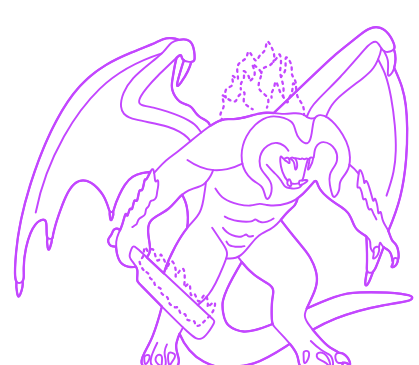
\includegraphics[width=5cm]{tmp/balrog.png}\end{center}}
\newcommand{\youshallnotpass}{\noindent{\color{purple}Attention Manue je m'en suis arrêté là :)}\begin{center}
\includegraphics[width=5cm]{tmp/gandalf.png}\end{center}}
% We use colors in equations to help readability.
% Un-comment next lines if you want just black text.
%\let\oldtextcolor\textcolor
%\renewcommand{\textcolor}[2]{\oldtextcolor{black}{#2}}

\newcommand{\RPC}{\mathrm{RPC}}
\newcommand{\M}{\mathfrak{M}}
\newcommand{\X}{\mathcal{X}}
\newcommand{\low}{\underline{P}}
\newcommand{\tdt}{\times\dots\times}
\newcommand{\enum}{, ~\dots, ~}
\newcommand{\opi}{[\![}
\newcommand{\cli}{]\!]}
\newcommand{\Bel}{\mathrm{Bel}}
\newcommand{\Pl}{\mathrm{Pl}}
\newcommand{\Nec}{\mathrm{Nec}}

\newcommand{\rowcol}{row, ~col}
\newcommand{\AD}{\mathrm{AD}}
\newcommand{\SAD}{\mathrm{SAD}}
\newcommand{\DSM}{\mathrm{DSM}}

\newcommand{\N}{\mathcal{N}}
\newcommand{\ith}{\textsuperscript{th}~}

\DeclareMathOperator{\CDF}{cdf}
\tikzset{
    declare function={
        cdf_erf(\x,\m,\s)=1/(1 + exp(-0.07056*((\x-\m-3)/\s)^3 - 1.5976*(\x-\m-3)/\s));
    }
}
\DeclareMathOperator*{\argmin}{arg\,min} % thin space, limits underneath in displays
\DeclareMathOperator*{\argmax}{arg\,max} % thin space, limits underneath in displays
\DeclareMathOperator*{\mean}{mean}
\DeclareMathOperator*{\median}{median}

%%%%%%%%%%%%%%%%% Defining the properties of the frames for theorems etc %%%%%%%%%%%%%%%%%%%%%%%%%%%%%%%%%%%%%
\mdfsetup{skipabove=\topskip, skipbelow=\topskip}  % Define Skips between the frames and text above and bellow

%% Code taken almost directly from https://ctan.mines-albi.fr/macros/latex/contrib/mdframed/mdframed-example-default.pdf
%% Theorem environment
\newcounter{theor}
\renewcommand{\thetheor}{\arabic{theor}}
\newenvironment{theorem}[1][]{%
  \refstepcounter{theor}%
  \ifstrempty{#1}%
  {\mdfsetup{%
    frametitle={%
       \tikz[baseline=(current bounding box.east),outer sep=0pt]
        \node[anchor=east,rectangle,fill=blue!30!white]
        {\strut Theorem~\thetheor};}}
  }%
  {\mdfsetup{%
     frametitle={%
       \tikz[baseline=(current bounding box.east),outer sep=0pt]
        \node[anchor=east,rectangle,fill=blue!30!white]
        {\strut Theorem~\thetheor:~#1};}}%
   }%
   \mdfsetup{innertopmargin=10pt,linecolor=blue!70!black,%
             linewidth=2pt,topline=true,
             frametitleaboveskip=\dimexpr-\ht\strutbox\relax,
             backgroundcolor=blue!10!white,%
             roundcorner=10pt,}
   \begin{mdframed}[]\relax%
   }{\end{mdframed}}

%% Definition environment
\newcounter{definition}
\renewcommand{\thedefinition}{\arabic{definition}}
\newenvironment{definition}[1][]{%
 \refstepcounter{definition}%
  \ifstrempty{#1}%
  {\mdfsetup{%
    frametitle={%
       \tikz[baseline=(current bounding box.east),outer sep=0pt]
        \node[anchor=east,rectangle,fill=blue!20]
        {\strut Definition~\thedefinition};}}
  }%
  {\mdfsetup{%
     frametitle={%
       \tikz[baseline=(current bounding box.east),outer sep=0pt]
        \node[anchor=east,rectangle,fill=blue!20]
        {\strut Definition~\thedefinition:~#1};}}%
   }%
   \mdfsetup{innertopmargin=10pt,linecolor=blue!20,%
             linewidth=2pt,topline=true,%
             frametitleaboveskip=\dimexpr-\ht\strutbox\relax,%
             backgroundcolor=blue!1!white,%
             roundcorner=5pt,}
   \begin{mdframed}[]\relax%
   }{\end{mdframed}}

%% Proposition environment
\newcounter{proposition}
\renewcommand{\theproposition}{\arabic{proposition}}
\newenvironment{proposition}[1][]{%
 \refstepcounter{proposition}%
 \mdfsetup{outerlinewidth=1,%
           roundcorner=10pt,%
           backgroundcolor=gray!5!white,%
           outerlinecolor=black,%
           innertopmargin=\topskip,%
           splittopskip=\topskip,%
           }
 \ifstrempty{#1}%
 {\begin{mdframed}[]\textbf{Proposition~\theproposition:~}\relax}%
 {\begin{mdframed}[]\textbf{Proposition~\theproposition:}~\textit{#1}\par\relax}%
 }{\end{mdframed}}


%% Example Environment
%\theoremstyle{definition}  % Boldface title, Roman body
%\newmdtheoremenv[roundcorner=5pt, font=\bfseries]{example}{Example}[section]
% OR
\newcounter{example}
\renewcommand{\theexample}{\arabic{example}}
\newenvironment{example}[1][]{%
 \refstepcounter{example}%
 \mdfsetup{roundcorner=5pt,}
 \ifstrempty{#1}%
 {\begin{mdframed}[]\textbf{Example~\theexample:~}\relax}%
 {\begin{mdframed}[]\textbf{Example~\theexample:}~\textit{#1}\par\relax}%
 }{\end{mdframed}}

% Remark Environment
\newenvironment{remark}{%
   \mdfsetup{hidealllines=true,%
             leftline=true,%
             linecolor=gray,%
             middlelinewidth=.2em,%
            }
   \begin{mdframed}[]\textbf{Remark:}\relax%
   }
   {\end{mdframed}}
   
   
% Redefines the proof environment
\renewenvironment{proof}{%
   \mdfsetup{hidealllines=true,%
             leftline=true,%
             linecolor=gray!50,%
             middlelinewidth=.2em,%
            }
   \begin{mdframed}[]\textit{\textbf{Proof:}}\relax%
   }
   {\qed\end{mdframed}}
%%%%%%%%%%%%%%%%%%%%%%%%%%%%%%%%%%%%%%%%%%%%%%%%%%%%%%%%%%%%%%%%%%%%%%%%%%%%%%%%%%%%%%%%%%%%%%%%%%%%%%%%%%%%%%%%%%%%%
   
   
% From CVPR cvpr.sty
\makeatletter
\DeclareRobustCommand\onedot{\futurelet\@let@token\@onedot}
\def\@onedot{\ifx\@let@token.\else.\null\fi\xspace}

\def\eg{\emph{e.g}\onedot} \def\Eg{\emph{E.g}\onedot}
\def\ie{\emph{i.e}\onedot} \def\Ie{\emph{I.e}\onedot}
\def\cf{\emph{cf}\onedot} \def\Cf{\emph{Cf}\onedot}
\def\etc{\emph{etc}\onedot} \def\vs{\emph{vs}\onedot}
\def\st{\emph{s.t}\onedot}
\def\wrt{w.r.t\onedot} \def\dof{d.o.f\onedot}
\def\iid{i.i.d\onedot} \def\wolog{w.l.o.g\onedot}
\def\etal{\emph{et al}\onedot}
\def\vs{\emph{vs}\onedot}

\def\blankpage{\newpage\null\thispagestyle{empty}\newpage}

\makeatother

%========================= Glossary ====================================

\pdfstringdefDisableCommands{%
  \def\glspl#1{<#1>}} % To silence hyperref Warning Token not allowed in a PDF string (Unicode)
%=======================================================================
%=======================================================================

\makeglossaries
\makeglossaries
\newglossaryentry{EO}
{%
    name={Earth Observation},
    description={Earth Observation involves employing remote sensing techniques for terrestrial, marine, and atmospheric monitoring}
}

\newglossaryentry{DISPARITY}
{%
    name={Disparity},
    description={The displacement of an object between two stereo images when expressed in pixels}
}

\newglossaryentry{DSM}
{%
    name=Digital Surface Model,
    description={Representation of the elevation of an area using a raster, including the vegetation, buildings \etc. Also called Digital Elevation Model. Sometimes referred to as a 2.5D model, as it is a 2D grid where each cell contains data about the elevation}
}

\newglossaryentry{DTM}
{%
    name={Digital Terrain Model},
    description={Representation of the terrain of an area using a raster, excluding the vegetation and buildings}
}

\newglossaryentry{LiDAR}
{%
    name={Light Detection And Ranging},
    description={Sometimes referred to as Laser Imaging Detection And Ranging. A LiDAR is an active sensor allowing to determine the distance between the sensor and its surroundings by measure the time between the emission of a laser beam and the detection of its reflection on the environment}
}

\newglossaryentry{Panchromatic}
{%
    name={Panchromatic image},
    description={A panchromatic image is an image representing the light in the visible spectrum, resulting in a black and white image. Satellites equipped with panchromatic sensors usually produce images of higher resolution than classical RGB sensors, although a high resolution RGB image can be obtained from a panchromatic image using a method called pansharpening}
}
\newacronym{b/h}{B/H}{Base-to-Height ratio}
\newacronym{cnes}{CNES}{Centre National d'Etudes Spatiales}
\newacronym{co3d}{CO3D}{Constellation Optique 3D}
\newacronym{dem}{DEM}{Digital Elevation Models}
\newacronym{dsm}{DSM}{Digital Surface Model}
\newacronym{dtm}{DTM}{Digital Terrain Model}
\newacronym{gis}{GIS}{Geographic Information Systems}
\newacronym{nir}{NIR}{Near Infra Red}
\newacronym{rgb}{RGB}{Red Green Blue}
\newacronym{vhr}{VHR}{Very High Resolution}
\newacronym{eo}{EO}{Earth Observation}
\newacronym{lidar}{LiDAR}{Light Detection And Ranging}
\newacronym{rpc}{RPC}{Rational Polynomial Models}
\newacronym{sgm}{SGM}{Semi-Global Matching}
\newacronym{cars}{CARS}{Chaîne Automatique de Restitution Stéréoscopique}
\begin{document}

    \definecolor{color}{HTML}{F5F5F5}
    \definecolor{ForestGreen}{HTML}{228B22}
    %======================= Page de Garde =================================
    \thispagestyle{empty}
    \setkeys{Gin}{draft=true}
    \begin{titlepage}
    \begin{center}
        \vspace*{1cm}
            
        \Huge
        \textbf{Caractérisation de l'incertitude au sein d'une chaîne de reconstruction 3D par stéréophotogrammétrie à partir d'images satellites}
            
        \vspace{0.5cm}
        \LARGE
        Uncertainty characterisation in a 3D stereo-photogrammetry pipeline using satellite images
            
        \vspace{1.5cm}
        \Large
        \textbf{Roman MALINOWSKI}
        \vspace{0.8cm}
            
        A thesis presented under the supervision of:\\
        Sébastien DESTERCKE\\
        and\\
        Emmanuel DUBOIS, Loïc DUMAS, Emmanuelle SARRAZIN
       
        \vfill
                
        \large
        Centre National D'Etudes Spatiales\\
        CS\\
        Heudiasyc - Université de Technologie de Compiègne\\
        ~\\
        30/06/2024

        \begin{figure}[h!]
            \begin{minipage}{0.25\linewidth}
                \vspace{0.6cm}
                \centering
\includegraphics[width=\linewidth]{Images/General/Logo_CS.png}
            \end{minipage}
            \begin{minipage}{0.48\linewidth}
                \centering
\includegraphics[width=\linewidth]{Images/General/Logo_CNES.png}
            \end{minipage}
            \begin{minipage}{0.25\linewidth}
                \vspace{0.6cm}
                \centering
\includegraphics[width=\linewidth]{Images/General/Logo_UTC.jpg}
            \end{minipage}
        \end{figure}
    \end{center}
\end{titlepage}
    \blankpage
    \chapter*{Remerciements}
    %==================== Glossaire, TOC etc ===============================
    \tableofcontents
    \thispagestyle{empty}
    \pagebreak

    \pagenumbering{Alph}  % Switch Numerotation of pages to uppercase letters
    \setcounter{page}{0}  % Resetting the page number
    \printglossary[type=\acronymtype,nonumberlist]
    \pagebreak
    
    %========================== Les choses sérieuses commencent ===========
    
    \pagenumbering{arabic}  % Switch numerotation of pages to Arabic
    %\doublespacing
    \onehalfspace
    
    \setkeys{Gin}{draft=true}
    \chapter*{Résumé}\addcontentsline{toc}{chapter}{Résumé}
\newpage

\chapter*{Abstract}\addcontentsline{toc}{chapter}{Abstract}
\newpage

\chapter*{Foreword}\addcontentsline{toc}{chapter}{Foreword}
Before delving into the subject of this manuscript, we would like to give some advise on how to efficiently navigate through it. When writing this thesis, we made extensive use of the \textit{hyperref} package, so that reading it on a PDF viewer was made easier. You can thus click on citations, figure numbers, equation numbers, chapters and sections number, acronyms \etc to directly jump to the concerned part. When following a reference to a citation, a previous chapter, equations or figures located in a different part of the manuscript, it can be a laborious process to go back to the section you were reading. Depending on the OS of you computer and the app used to read the PDF document, there usually exist shortcuts to jump back to the previous view. This allows to quickly switch back and forth between chapters and sections.

For instance, imagine that you are in \Cref{chap:epistemic_uncertainty} and we make a reference to an equation form \Cref{chap:representation_of_uncertainty}. If you do not recall the equation, and quickly want to see what it is about, just click on the hyperlink to directly go to the relevant equation from \Cref{chap:representation_of_uncertainty}. Then use your system's shortcut to go back to where you were in \Cref{chap:epistemic_uncertainty}. 
\begin{itemize}
    \item Using Acrobat Reader: the short cut \keys{\Altwin + \arrowkeyleft} (left arrow key) on Windows or Linux brings you to the previous view after clicking on a hyperlink. Afterwards, you can alternate views with \keys{\Altwin + \arrowkeyright} and \keys{\Altwin + \arrowkeyleft}. On MacOS, the \keys{\Altwin} key is replaced by the \keys{\cmd} key.
    \item Using Preview on MacOS, you can add the \menu{Page History} button to the toolbar, by right-clicking on the toolbar and selecting \menu{Customize Toolbar}
    \item Using Okular on Linux, \keys{\Altwin + \shift + \arrowkeyleft} (left arrow key) brings you to the previous view after clicking on a hyperlink. Afterwards, you can alternate views with \keys{\Altwin + \shift + \arrowkeyright} and \keys{\Altwin + \shift + \arrowkeyleft}
\end{itemize}
Hopefully, this makes the reading of this thesis a more pleasant experience.

\newpage
\renewcommand{\epigraphsize}{\normalsize}
\setlength{\epigraphrule}{1pt}
\setlength{\epigraphwidth}{0.48\linewidth}
\vspace*{\fill}
\epigraph{You never talk of likelihoods on Arrakis.\\You speak only of possibilities.}{Frank Herbert, \textit{Dune}}
\vspace*{\fill}

\newpage

    \setkeys{Gin}{draft=true}
    \chapter*{Introduction}\addcontentsline{toc}{chapter}{Introduction}
Knowing the Earth's topography is crucial for modern geosciences. Depending on the level of details needed, different models can be used: the Earth ellipsoid, its geoid (gravity equipotential surface), topography maps (\ie contour lines of hiking maps) \etc One of those models is the \acrfull{dsm}, which is a representation of a surface's elevation on a regular grid. This type of model appears as a natural solution in many \acrfull{gis}. Indeed, they can easily be handled and provide georeferenced information regarding the topography of an area. \Cref{fig:intro_dsm_example} presents an example of a \acrshort{dsm}.

\acrshort{dsm}s find usage in various contexts and for a wide range of applications. In \acrfull{eo} for instance, \acrshort{dsm}s are used to monitor changes in vegetation \cite{sadeghi_canopy_2016}, melting rates of glaciers \cite{berthier_glacier_2014} or water resources \cite{yamazaki_merit_2019}. \acrshort{dsm}s can also be employed for catastrophe management, for instance to predict the potential damage caused by earthquakes or floods \cite{jenkins_physics-based_2023}. \acrshort{dsm}s are also crucial for ortho-rectifying images, \ie geometrically correcting the effects of distortion due to the sensor's angle of view and the terrain's topography. Finally, high resolution \acrshort{dsm} can help drone navigation in urban settings, for Defense applications, or more broadly for urban planning \cite{velazco_3d_2012}.

\begin{figure}
    \centering
    \begin{subfigure}[t]{0.5\linewidth}
        \centering
        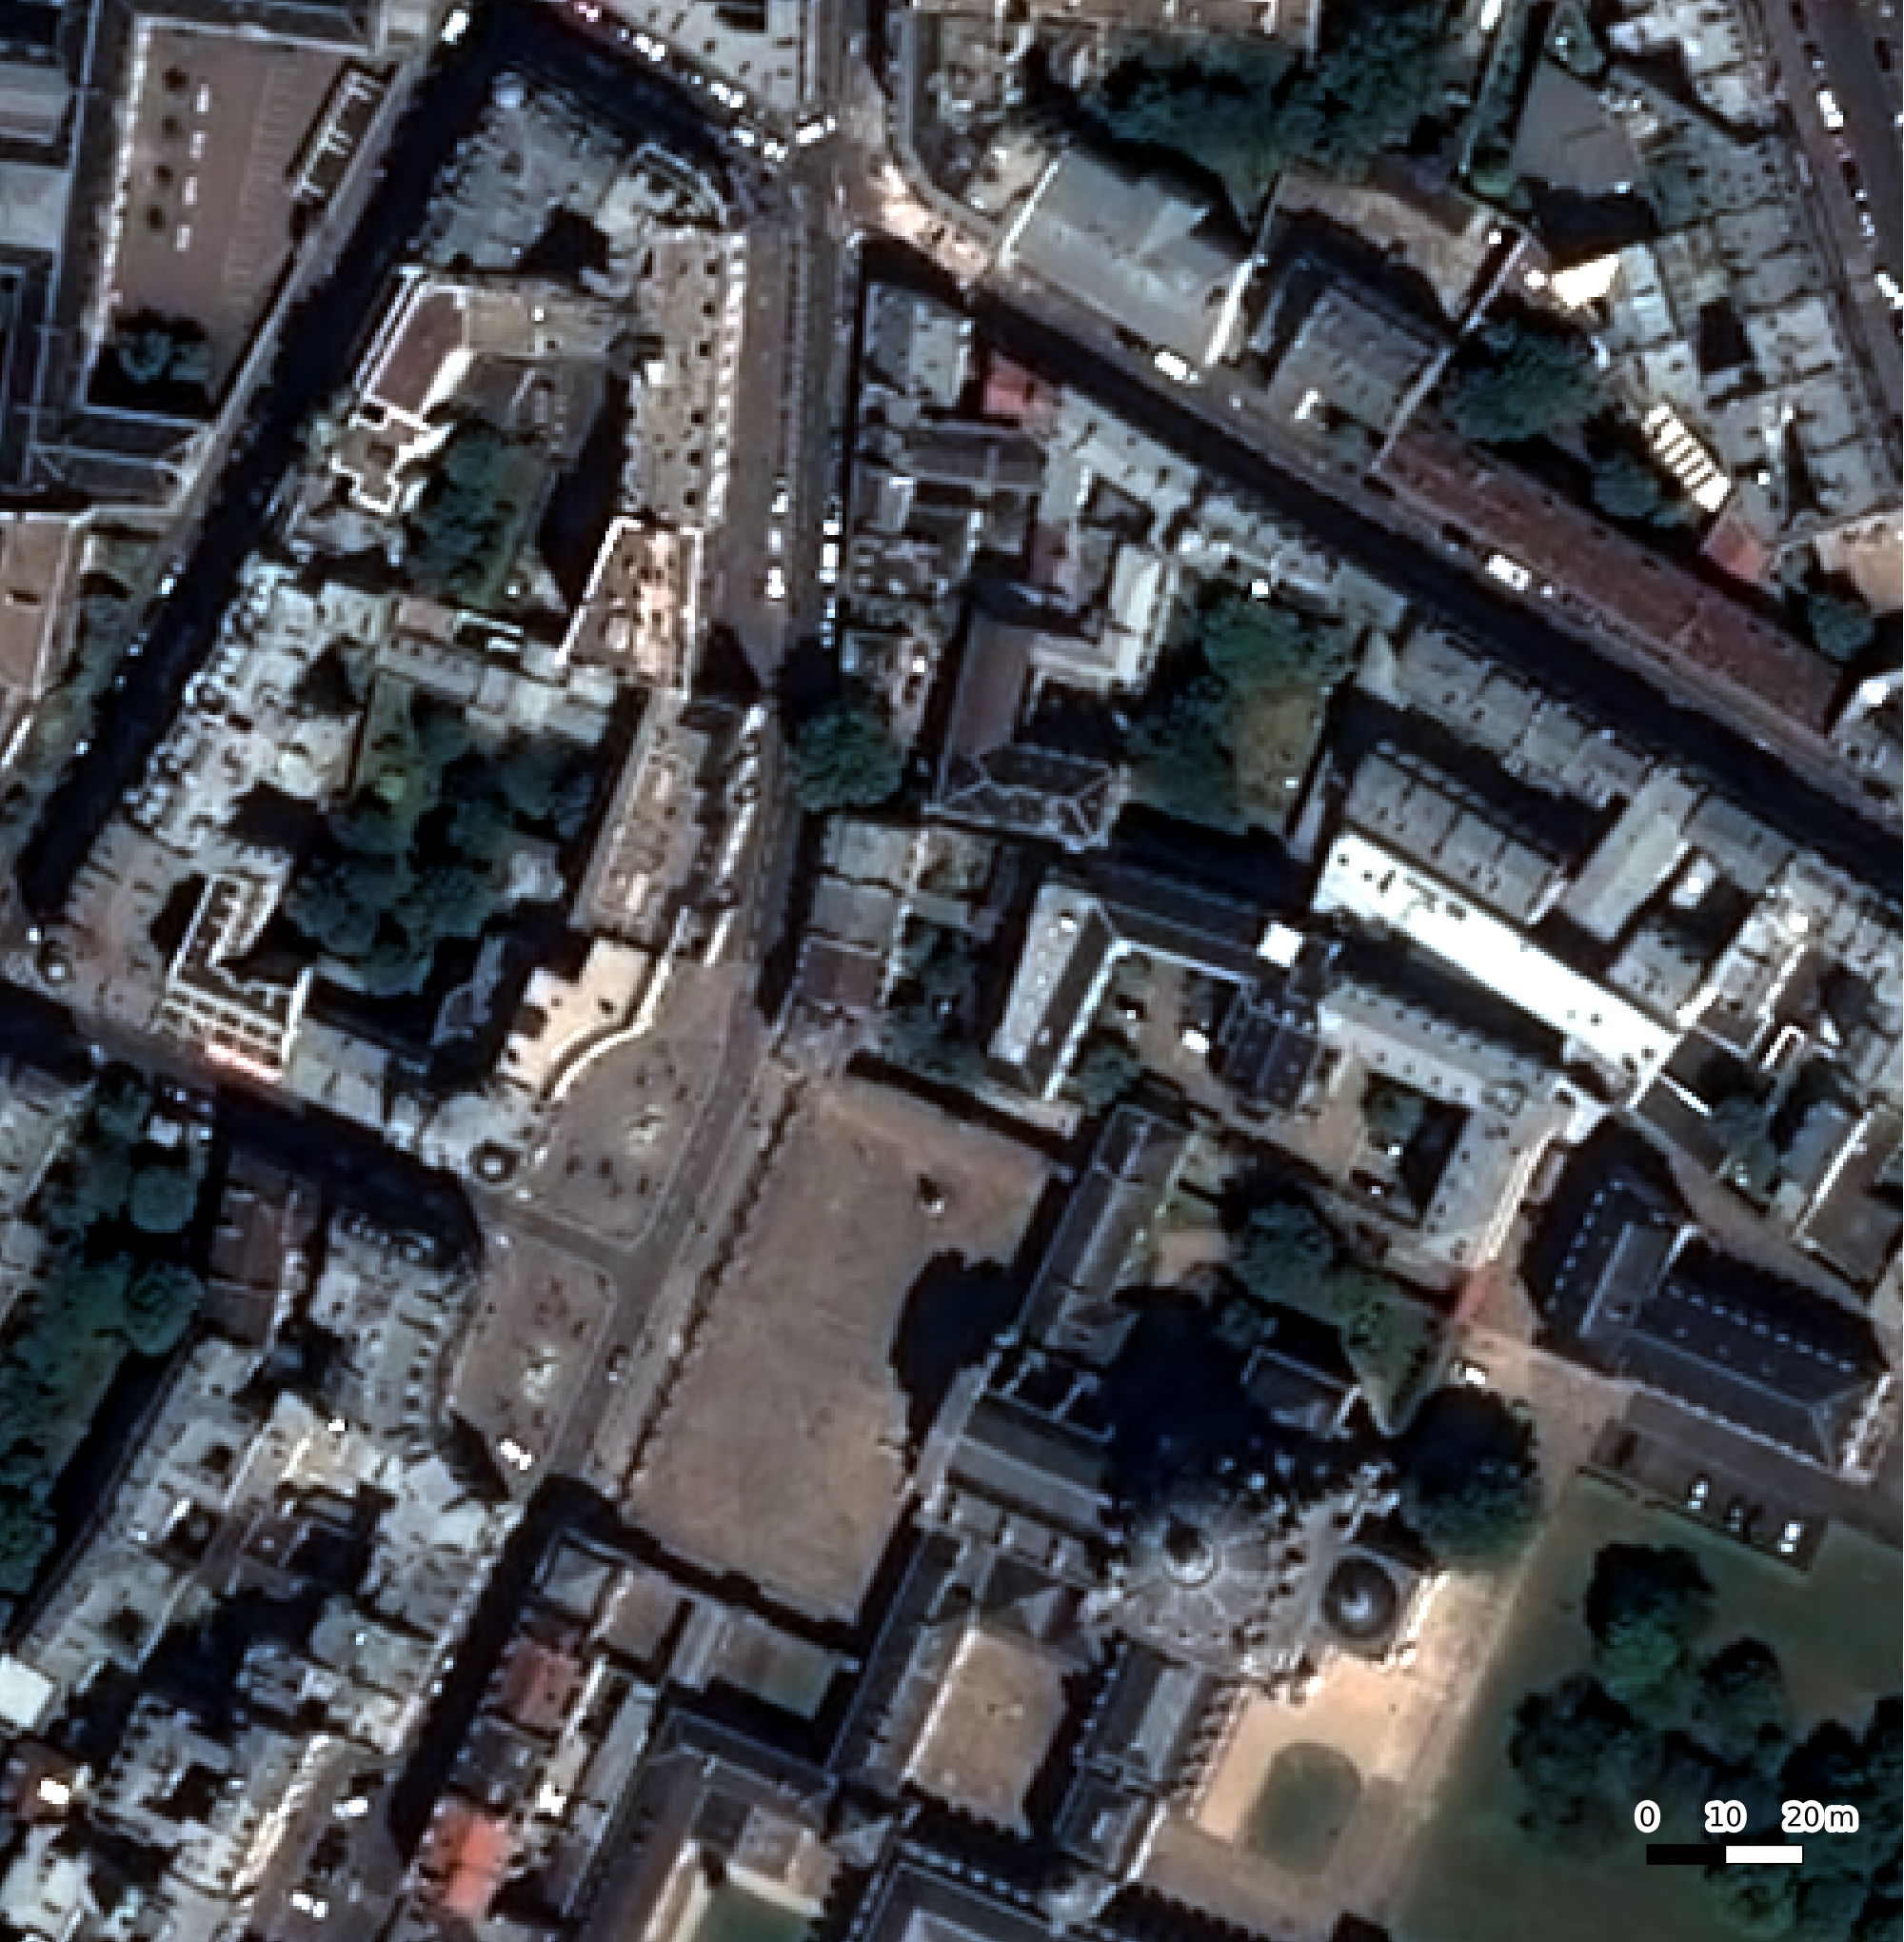
\includegraphics[height=6cm]{Images/0_Intro/Paris_Ortho.png}
        \caption{Pléiades image \copyright \acrshort{cnes} 2017, Distribution AIRBUS DS}
        \label{fig:VDG_ortho}
    \end{subfigure}\hfill
    \begin{subfigure}[t]{0.5\linewidth}
        \centering
        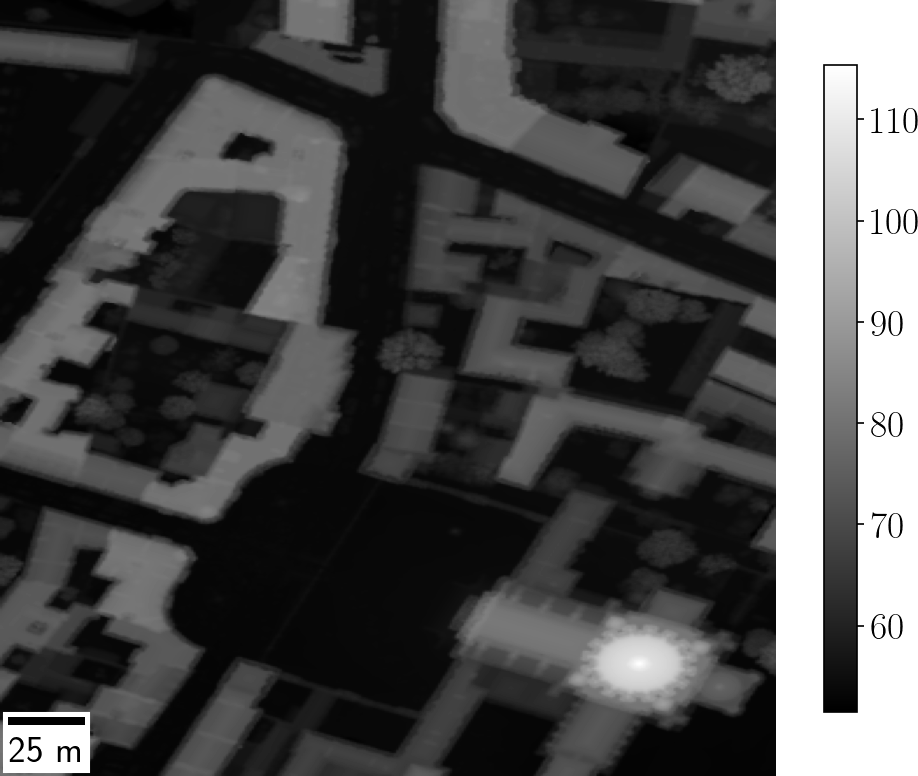
\includegraphics[height=6cm]{Images/0_Intro/Paris_DSM.png}
        \caption{Digital Surface Model from LiDAR HD (unit: m)}
        \label{fig:VDG_dsm}
    \end{subfigure}
    \caption{Satellite image over Val-de-Grâce, Paris at $0.5$m of resolution, and a \acrshort{dsm} over the same area.}
    \label{fig:intro_dsm_example}
\end{figure}

There are multiple ways of creating a \acrshort{dsm} from airborne sensors such as planes, drones or satellites. The first way is to use \acrshort{radar} interferometry, as done by Sentinel-1 satellites \cite{geudtner_sentinel-1_2014}, the Shuttle Radar Topography Mission (SRTM) \cite{farr_shuttle_2007} or TanDEM-X (\cite{krieger_tandem-x_2007}). Typical planimetric resolutions obtained are in the range of a dozen meters (10m for TanDEM-X or 30m for the SRTM). Another method is to construct \acrshort{dsm} by means of stereophotogrammetry \cite{tao_comprehensive_2001}, \ie the science of recovering 3D information from optical images. For this method, images of a scene are acquired from different points of view. Depth information is recovered from the parallax effect between images, \ie the fact that objects closer to the sensors present a greater shift between images than objects in the background. This effect is also what allows depth perception in human vision. \Cref{fig:parallax} illustrates the parallax effect, where the top of Eiffel Tower has a greater position shift in both image than its basis. As current optical satellites have a sub-meter resolution, it is possible to massively produce \acrshort{dsm} covering the globe using photogrammetry for a relatively low cost. The altimetric resolution is typically around one meter, although it depends of the different acquisition angles of the satellites. A final method for producing \acrshort{dsm} is to use LiDAR (laser sensors) \cite{khosravipour_generating_2016}. Using LiDAR allows to obtain very good accuracy. For instance, the french institute IGN (\textit{Institut national de l'information Géographique et forestière}) is using LiDAR to cover the french territory, with a planimetric accuracy of 25 centimeters, and an altimetric resolution of 5 centimeters allowing to observe very small objects. Acquisitions campaigns such as this one are carried out using airborne vehicles, and are thus costly and take a lot of time. Therefore, photogrammetry \acrshort{dsm}s are currently the best solution to produce \acrshort{dsm}s covering the globe  with a sub-meter resolution for relatively low costs. This thesis will therefore mainly considered \acrshort{dsm}s produced using stereophotogrammetry.

\begin{figure}
    \begin{subfigure}[t]{0.32\linewidth}
        \flushleft
        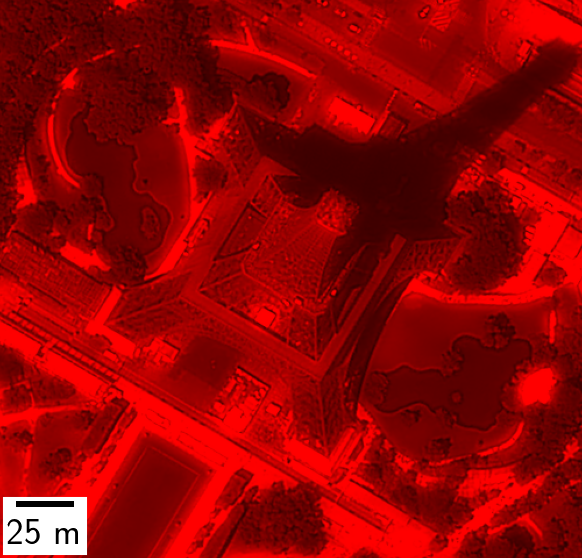
\includegraphics[width=\linewidth]{Images/0_Intro/eiffel_tower_left.png}
        \caption{Left Image (Red channel)}
        \label{fig:eiffel_tower_left}
    \end{subfigure}\hfill
    \begin{subfigure}[t]{0.32\linewidth}
        \centering
        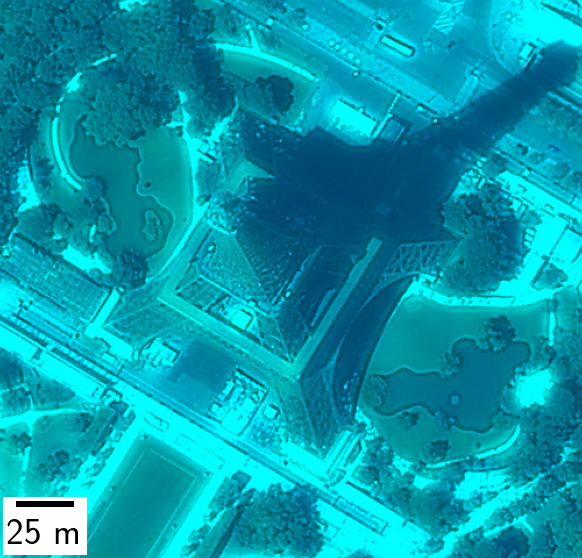
\includegraphics[width=\linewidth]{Images/0_Intro/eiffel_tower_right.png}
        \caption{Right Image (Blue and Green channel)}
        \label{fig:eiffel_tower_right}
    \end{subfigure}\hfill
    \begin{subfigure}[t]{0.32\linewidth}
        \flushright
        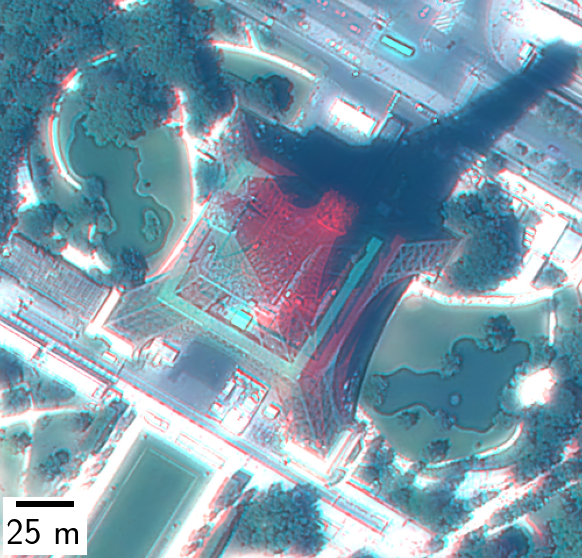
\includegraphics[width=\linewidth]{Images/0_Intro/eiffel_tower_ana.png}
        \caption{Anaglyph}
        \label{fig:eiffel_tower_ana}
    \end{subfigure}
    \caption{Example of the parallax effect: the top of the Eiffel Tower has a greater shift in-between images than its basis. The anaglyph contains the red band of the left image and the green and blue bands of the right image. (Pléiades © \acrshort{cnes} 2023, Distribution AIRBUS DS)}
    \label{fig:parallax}
\end{figure}


In this context, \acrshort{cnes} - the French Space Agency - is planning to launch 4 low-cost optical satellites with Airbus Defense and Space, in order to massively produce \acrshort{dsm} using stereophotogrammetry. This mission, named \acrshort{co3d} (for \textit{Constellation Optique 3D}, \cite{melet_co3d_2020}), was conceived jointly with IGN to provide high resolution \acrshort{dsm} over the globe, at a $50cm$ resolution.

For thus purpose, \acrshort{cnes} developed a pipeline dedicated to process all images provided by the \acrshort{co3d} satellites automatically and at a very large scale. This pipeline is called CARS (``Chaine Automatique de Restitution par Stéréoscopie''), and is composed of many different image processing steps. The different steps will be detailed in the first chapter, but can be summarized as follows:
\begin{itemize}
    \item Resampling of image in a convenient geometry for matching pixels
    \item Dense matching of every pixel between stereo images
    \item Triangulation of matched pixels into 3D points
    \item Rasterization, \ie projection of the 3D points onto a regular grid, therefore yielding the final \acrshort{dsm} 
\end{itemize}
The hardest and most crucial part of this pipeline is the dense matching of pixels. It is also a famous problem in computer vision, which find applications in robotics and autonomous cars for instance \cite{geiger_vision_2013}. Alongside the \acrshort{dsm} computation, one of the requirements of the \acrshort{co3d} mission is to produce a performance map indicating the estimated quality of each cell of the \acrshort{dsm}. This motivates \acrshort{cnes} to lead research in order to estimate the uncertainty amongst the CARS pipeline. The main objective of this thesis is therefore to characterize and propagate the uncertainty throughout this photogrammetry pipeline. Considering the complexity of the \acrshort{cars} pipeline, as well as the time constraint resulting from the future launch of the \acrshort{co3d} satellites, we mainly focus on characterizing the uncertainty of the dense matching step. After quantifying this uncertainty, we propagate it to the end of the pipeline onto the final \acrshort{dsm}.

Characterizing and quantifying uncertainty has many benefits, although it can sometimes be computationally expensive to deal with. It indeed provides additional information for better decision making and risk management. It can also allow for a better understanding of the underlying processes at stake regarding the value of interest. In many cases, uncertainty estimation is treated as a secondary objective in applications. However, jointly estimating a value and its uncertainty can lead to new strategies to reduce the uncertainty or sometimes even improve the performances of the main applications \cite{chen_learning_2023,jiang_unsupervised_2024}.

Before delving into uncertainty estimation and its propagation, we first need to specify what we mean by uncertainty. Uncertainty is a situation where a measure or value of interest is not known, or not known with precision. It is subject to change, as additional information, measures or a different acquisition protocol may reduce how uncertain a value is. It can also be subjective. For instance, someone may be uncertain about the launch date of \acrshort{co3d} satellites, while someone else working at the launch pad might have the answer. This highlights the fact that while everyone has an understanding of what uncertainty is, it encompasses very different concepts in nature. It is common to differentiate the various types of uncertainty by dividing it into two categories: stochastic uncertainty (also called random uncertainty) and epistemic uncertainty \cite{hora_aleatory_1996,frank_treatment_1999}.

Stochastic uncertainty refers to every situation of purely aleatoric nature. For instance, the result of a coin throw, random noise on a CCD captor or the Brownian movement of a particle. An operator typically encounters this kind of uncertainty in a situation where they have access to many measures or observations of the same value of interest. It is usually modeled mathematically with a frequentist approach, using probability measures such as the uniform distribution, Gaussian distribution or the Student's $t$ distribution.

On the other hand, epistemic uncertainty refers to a situation where the value of interest is not known or ill-known due to a lack of knowledge. Think of the previous example with the launch date of satellites, or if someone was asked to guess Io's mass, one of the moons of Jupiter. There is no random process at stake here, and there is usually no point of acquiring multiple samples of the measure if we have a reliable and precise sensor. Once the value of interest is known, the uncertainty no longer exists. It has been proposed to model this kind of uncertainty using a Bayesian approach for probability, by opposition with the frequentist approach. Probabilities here represent a state of knowledge, or degree of belief, one has over the value of interest. It can be updated with additional knowledge, thus leading to the notion of prior and posterior probabilities. We will see during this thesis that other model can be used to characterize this uncertainty, for instance \textit{imprecise probabilities} and more specifically \textit{possibility distributions}. In satellite imagery, those models have been used to detect land changes \cite{lesniewska-choquet_specialite_2020} for instance.

During this thesis, we contributed both to the field of photogrammetry and to the field of imprecise probabilities. Here is a quick overview of the contents that can be found in the following chapters:
\begin{itemize}
    \item \Cref{chap:stereophotogrammetry} introduces the different stereophotogrammetry concepts considered in this thesis. It focuses on the stereo pipeline developed by \acrshort{cnes} and its sources of uncertainty, which will be considered in our applications.
    \item \Cref{chap:representation_of_uncertainty} will introduce the different uncertainty models considered in this thesis, mainly possibility distributions and copulas.
    \item In \Cref{chap:joining_credal_sets}, we propose different methods for creating specific multivariate uncertainty models based on the models introduced in \Cref{chap:representation_of_uncertainty}. We also study the relationships between the methods we introduced.
    \item \Cref{chap:propagating} uses the concepts of \Cref{chap:representation_of_uncertainty} and the results of \Cref{chap:joining_credal_sets} to propagate uncertainties modeled by possibility distributions in a part of the dense matching step of the stereo pipeline.
    \item \Cref{chap:epistemic_uncertainty} also uses possibility distributions, but this time to characterize the uncertainty of the dense matching step itself. Using this method, we are able to obtain confidence intervals at the end of the dense matching step. 
    \item \Cref{chap:elevation_intervals} propagates the disparity intervals to the end of the pipeline, in the form of elevation intervals on the final \acrshort{dsm}. 
\end{itemize}

As our contributions concern two distinct fields of research, multivariate uncertainty and photogrammetry, readers with a level of expertise in one field might be less interested in the second field. We tried, as much as possible, to write each chapter so it can be read and followed by everyone, although some details might need additional knowledge in a field of expertise. To help readers to navigate through chapters according to their center of interests, here is an attempt to classify each chapter into its field of research.
\begin{itemize}
    \item \Cref{chap:stereophotogrammetry} focuses on stereophotogrammetry.
    \item \Cref{chap:representation_of_uncertainty,chap:joining_credal_sets} focuses on the modelling of uncertainty, with \Cref{chap:joining_credal_sets} delving into more advanced concepts.
    \item \Cref{chap:propagating} joins both fields, but leans a bit more towards uncertainty propagation than towards photogrammetry. 
    \item \Cref{chap:epistemic_uncertainty,chap:elevation_intervals} also attempt to join both fields of research, but focuses almost completely on photogrammetry.
\end{itemize}

The rest of this section lists the contributions and research events that occurred during this thesis.
\noindent National conferences:
\begin{itemize}
    \item LFA 2022: ``Copules, probabilités inférieures et ensembles aléatoires : comment et quand les appliquer ?''  \cite{malinowski_copules_2022}
\end{itemize}
International conferences:
\begin{itemize}
    \item SMPS 2022: ``Copulas, Lower Probabilities and Random Sets: How and When to Apply Them?'' - \cite{malinowski_copulas_2022}
    \item ISIPTA 2023 (Special jury recognition Award): ``Uncertainty Propagation using Copulas in a 3D Stereo Matching Pipeline'' -  \cite{malinowski_uncertainty_2023}
    \item IGARSS 2024: ``Robust Confidence Intervals For Digital Surface Models Using Satellite Photogrammetry'' -  \cite{malinowski_robust_2024}
\end{itemize}
International journals:
\begin{itemize}
    \item International Journal of Approximate Reasoning: ``Uncertainty propagation in stereo matching using copulas'' -  \cite{malinowski_uncertainty_2024}
\end{itemize}
Not yet published pre-print:
\begin{itemize}
    \item Available on ArXiv: ``Robust Confidence Intervals in Stereo Matching using Possibility Theory'' - \cite{malinowski_robust_2024-1}
\end{itemize}
Workshops, poster sessions:
\begin{itemize}
    \item Belief 2022 conference: Poster presentation "Using Copulas with Random Sets"
    \item Workshop Imagin ``journée imprécision et incertitude en analyse et traitement d'images'': Funding of the event and communication, and oral presentation ``Uncertainty Propagation in Dense Matching''
    \item SFPT ``Pléiades Neo: de nouveaux satellites pour de nouveaux usages''. Oral presentation: ``Confidence Intervals for Digital Surface Models''
    \item GdR IASIS ``Télédétection et Climat''. Oral presentation ``Estimation d'Incertitudes dans la Création de Modèles Numériques de Surface issus d'Imagerie Spatiale''
\end{itemize}

\pagebreak

    
    \setkeys{Gin}{draft=false}
    \chapter{Introduction to Stereophotogrammetry}\label{chap:stereophotogrammetry}
\section{Digital Surface Models}\commanue{Là c'est en reprendre car tu as copié collé ce paragraphe dans l'intro donc à voir comment tu équilibres entre l'intro et ici. Ici il faudra plus détailler. Dans l'intro tu te limites à expliquer brivèevemnt un DSM, la différence avec un DTM (juste le sol), les différentes méthodes possibles avec leur niveau de résolution et le niveu de détail. Ici tu peux pousser la comparaison, tu peux montrer les différentes produits. Peut-être ici donner des exemples montrer une ville, genre toulouse,  avec différents DSM pour voir les différents niveaux de détails, parler des formats etc. Tu peux aussi parler de l'étendue spatiale des produits, de leur mise à jour. Pour l'instant pas mal d'interventions manuelles.}
\todoroman{Utiliser les slides de formation CARS pour montrer les différentes méthodes pour faire de la 3D, mettre des exmples de LiDAR ou faire un schéma ?}

\commanue{Il faudrait aussi montrer des résultats, en gros c'est quoi en fait un modèle 3D. Après parmi tous les exemples d'utilisation de la 3D que tu donnes tu peux en détailler un un peu plus. Celui que tu préfères.}
Knowing the Earth's topography is crucial for modern geosciences. As such, \acrfull{dsm}, which are a representation of a surface's elevation on a regular grid, appear as a natural solution in many \acrfull{gis}. Indeed, they can easily be handled and provide georeferenced information regarding the topography of an area. \acrshort{dsm} find usage in various contexts for a wide range of applications. In \acrfull{eo} for instance, \acrshort{dsm} are used to monitor changes in vegetation \cite{sadeghi_canopy_2016}, melting rates of glaciers \cite{berthier_glacier_2014, rieg_pleiades_2018}, volcanos \cite{ganci_data_2022}, snow or water resources \cite{marti_mapping_2016, gascoin_theia_2019, yamazaki_merit_2019} \etc Similarly, \acrshort{dsm} are employed for catastrophe management, to predict the potential damage caused by earthquakes or floods \cite{jenkins_physics-based_2023} \dots \acrshort{dsm} are also crucial for ortho-rectifying image, \ie geometrically correcting the effects of distortions between the sensor and the terrain. This process creates a planimetric image with a consistent scale in all parts of the image. It allows images to be easily used in \acrshort{gis} or as background for maps. In urban settings, high resolution \acrshort{dsm} can help drone navigation for Defense applications, or more broadly for urban planning \cite{velazco_3d_2012}.

Nowadays, \acrshort{dsm} are mostly generated from laser scanning with LiDAR sensors, radar interferometry or stereophotogrammetry \cite{youssefi_cars_2020}. Air-borne laser scanning results in \acrfull{vhr} models, but the swath width and cost of acquisition campaigns do not allow to periodically cover the globe\commanue{Pour le LIDAR tu peux citer le Liadr HD de l'IGN: durée de la campagne et données déjà disponible pour montrer que rien que pour avoir la France cela prend beaucoup de temps.}. Space-borne \acrshort{lidar} is mostly used for atmospheric measurements, or discrete measurements \cite{fouladinejad_history_2019}. For instance, NASA's ICESat-2 \cite{jasinski_atlasicesat-2_2020} measures elevation of seas and glaciers using 6 lasers taking measurements along track, which is not adapted for reconstructing high-accuracy DSM. Space-borne radar interferometry remains widely used, and has allowed to create a worldwide digital model of emerged surfaces of the Earth at $30$m and $90$m resolution with the SRTM mission \cite{farr_shuttle_2007}\commanue{Tu peux aussi citer le DEM Copernicus https://spacedata.copernicus.eu/collections/copernicus-digital-elevation-model il faudrait détailler comment il est réalisé. Le SRTM c'est la classe car c'est via la navette Endeavour. Pour revenir au DEM copernicus, il est réalisé à partir de Tandem-X qui est un SAR qui permet de réaliser des DEM jusqu'à 10 à 12m. En fonction du temps tu peux détailler un peu le principe d'acquisitions}. To obtain coarser resolutions\commanue{Donne des ordres de grandeurs qu'on vise par rapport aux autres technos}, it is possible to leverage the technological advancement of optical sensors in orbit to create sub-meter \acrshort{dsm} using stereophotogrammetry with relatively low cost\commanue{Peut-être détailler pourquoi c'est plus low cost}. However, this process is more complex than laser measurements as it deduces height from the principle of parallax. Stereophotogrammetry pipelines usually consists in multiple processing steps with intermediary products (see \ref{sec:classical_stero_pipeline}), with different methods, parameterization and post-processes available for each step (\eg matching, filtering \etc). This broad range of solutions allow to adapt our processes to the type of images and terrain observed, but it sometimes makes it difficult to determine the configuration producing the best quality DSM, or to single out a general good-working configuration. 

This thesis focuses on \acrshort{dsm} obtained from stereophotogrammetry, however we will use \acrshort{dsm} obtained from air-borne LiDAR acquisitions as references to validate our results, considering their high resolutions\commanue{Dans cette section tu mentionnes rapidement le lidar. Je pense que tu dois détailler un peu plus car c'est comme même ta vérité terrain. Il faadrait parler de l'acquisition, du format (points), de la rasterisation (on se retrouve avec plusieurs bandes). Il faudrait aussi citer le lidarHD de l'IGN car c'est vraiment cela que tu utilises comme VT. Tu peux mettre en perspective le temps nécessaire pour faire les acquisitions et mettre à dispo les produits. Notamment cela te sera utile quand tu aborderas la mission CO3D}.
\commanu{ pas plus que manue sur cette section, complètement d'accord}
\todoroman{Schema de \acrshort{dsm} par avion LiDAR, satellite interfero et stereo}
\section{CO3D mission and Pléiades Satellites}\label{sec:co3d}\commanue{Moi je mettrais un titre plus générique sur les satellites optiques haute résolution. Tu démarres par DSM dans la section précédente et tu mentionnes ce type de satellites pour créer des DSM. Donc section suivantes tu parles de ces satellites que l'on peut utiliser pour faire de la 3D (ah transition !) car ils possèdent des atouts : haute résolution, agilité. Tu peux mentionner ensuite les satellites existants Worldview Pleiades CSO (acquisition push-broom que tu peux introduire si tu veux) et ensuite tu introduis la nouvelle constellation de satellites CO3D matrice de bayer, ils volent en formation donc acquistion synchrone (pour une paire),etc. Te connaissant je ferais des sous-sections par exemple : intro globale sur les sat optiques HR, mission actuelles, mission CO3D, données que tu utilises}\commanu{+1}

The following paragraphs detail satellites characteristics relevant to stereophotogrammetry. It is important to notice that although the sensor used greatly determines the resolution of the final \acrshort{dsm}, it is not the only factor at stake here. The altitude and positions of the satellites are also crucial for the resolution\todoroman{parler de \cite{qin_critical_2019} avec un bon ratio et surtout la diff d'angles solaires}, and can be characterized by the \acrfull{b/h} ratio, as in \Cref{fig:RPC}. This ratio is computed by dividing the distance separating the stereo acquisitions by the altitude of the satellite. It indicates the angle formed between the line of sights originating from the satellites towards an object of the scene. A high \acrshort{b/h} allows for high elevation accuracy, but possesses more occluded regions (for instance a narrow street between two high buildings), and conversely for a low B/H \cite{delon_small_2007}.

The main source of images used in this thesis comes from Pléiades images\commanue{Tu peux mentionner çà à la fin de la section (tu sais le truc qui s'appelle une conclusion) une fois que tu as présenter les différentes mission et leur caractéristiques. Tu peux dire que bien que les travaux de cette thèse ont pour vocation de servir dans le segment-sol de CO3D en l'absence de donnée CO3D tu as utilisé des données Pléiades qui ont caractérisques assez proches.}. The Pléiades constellation developed by Airbus is composed of two identical satellites, 1A and 1B. The satellites were launched in 2011 and 2012 in an heliosynchronous orbit at $690$km, for both civilian and defense usages. They provide panchromatic images at a resolution of $70$cm (resampled at $50$cm), and RGB-NIR images at a resolution of $2$m, with a $20$km swath (\url{https://dinamis.data-terra.org/pleiades/}). Their high agility and revisit rate allow them to capture stereo and tri-stereo images for any location on the globe, ideal to produce \acrshort{dsm} with high accuracy\commanue{Il y a même un mode vidéo où tu prends plus d'une dizaine images}. The \acrshort{b/h} ratio for stereo acquisitions can vary between $0.1$ and $0.4$. However, stereo acquisitions is not the only objective of this mission, even though the demand for those products is increasing \cite{berthier_glacier_2014, poli_radiometric_2015, rieg_pleiades_2018, loghin_potential_2020}. The acquisition of stereo images is thus provided on command, which can conflict with other usages of the satellite, and can become costly when trying to cover large areas \commanue{Tu peux mentionner que c'est un satellite dual donc militaire et civil et que les militaires ont la priorité. Après tu peux aussi dire que Pléiades est utilisé lors de l'activation de la chartre https://disasterscharter.org/fr/web/guest/home. Alors on a pas déclenché la chartre mais pour le glissment de terrain dans le sud-est Pléiades avait pris de stéréo.}.  
\begin{figure}
    \centering
    \begin{subfigure}[t]{0.5\linewidth}
        \centering
        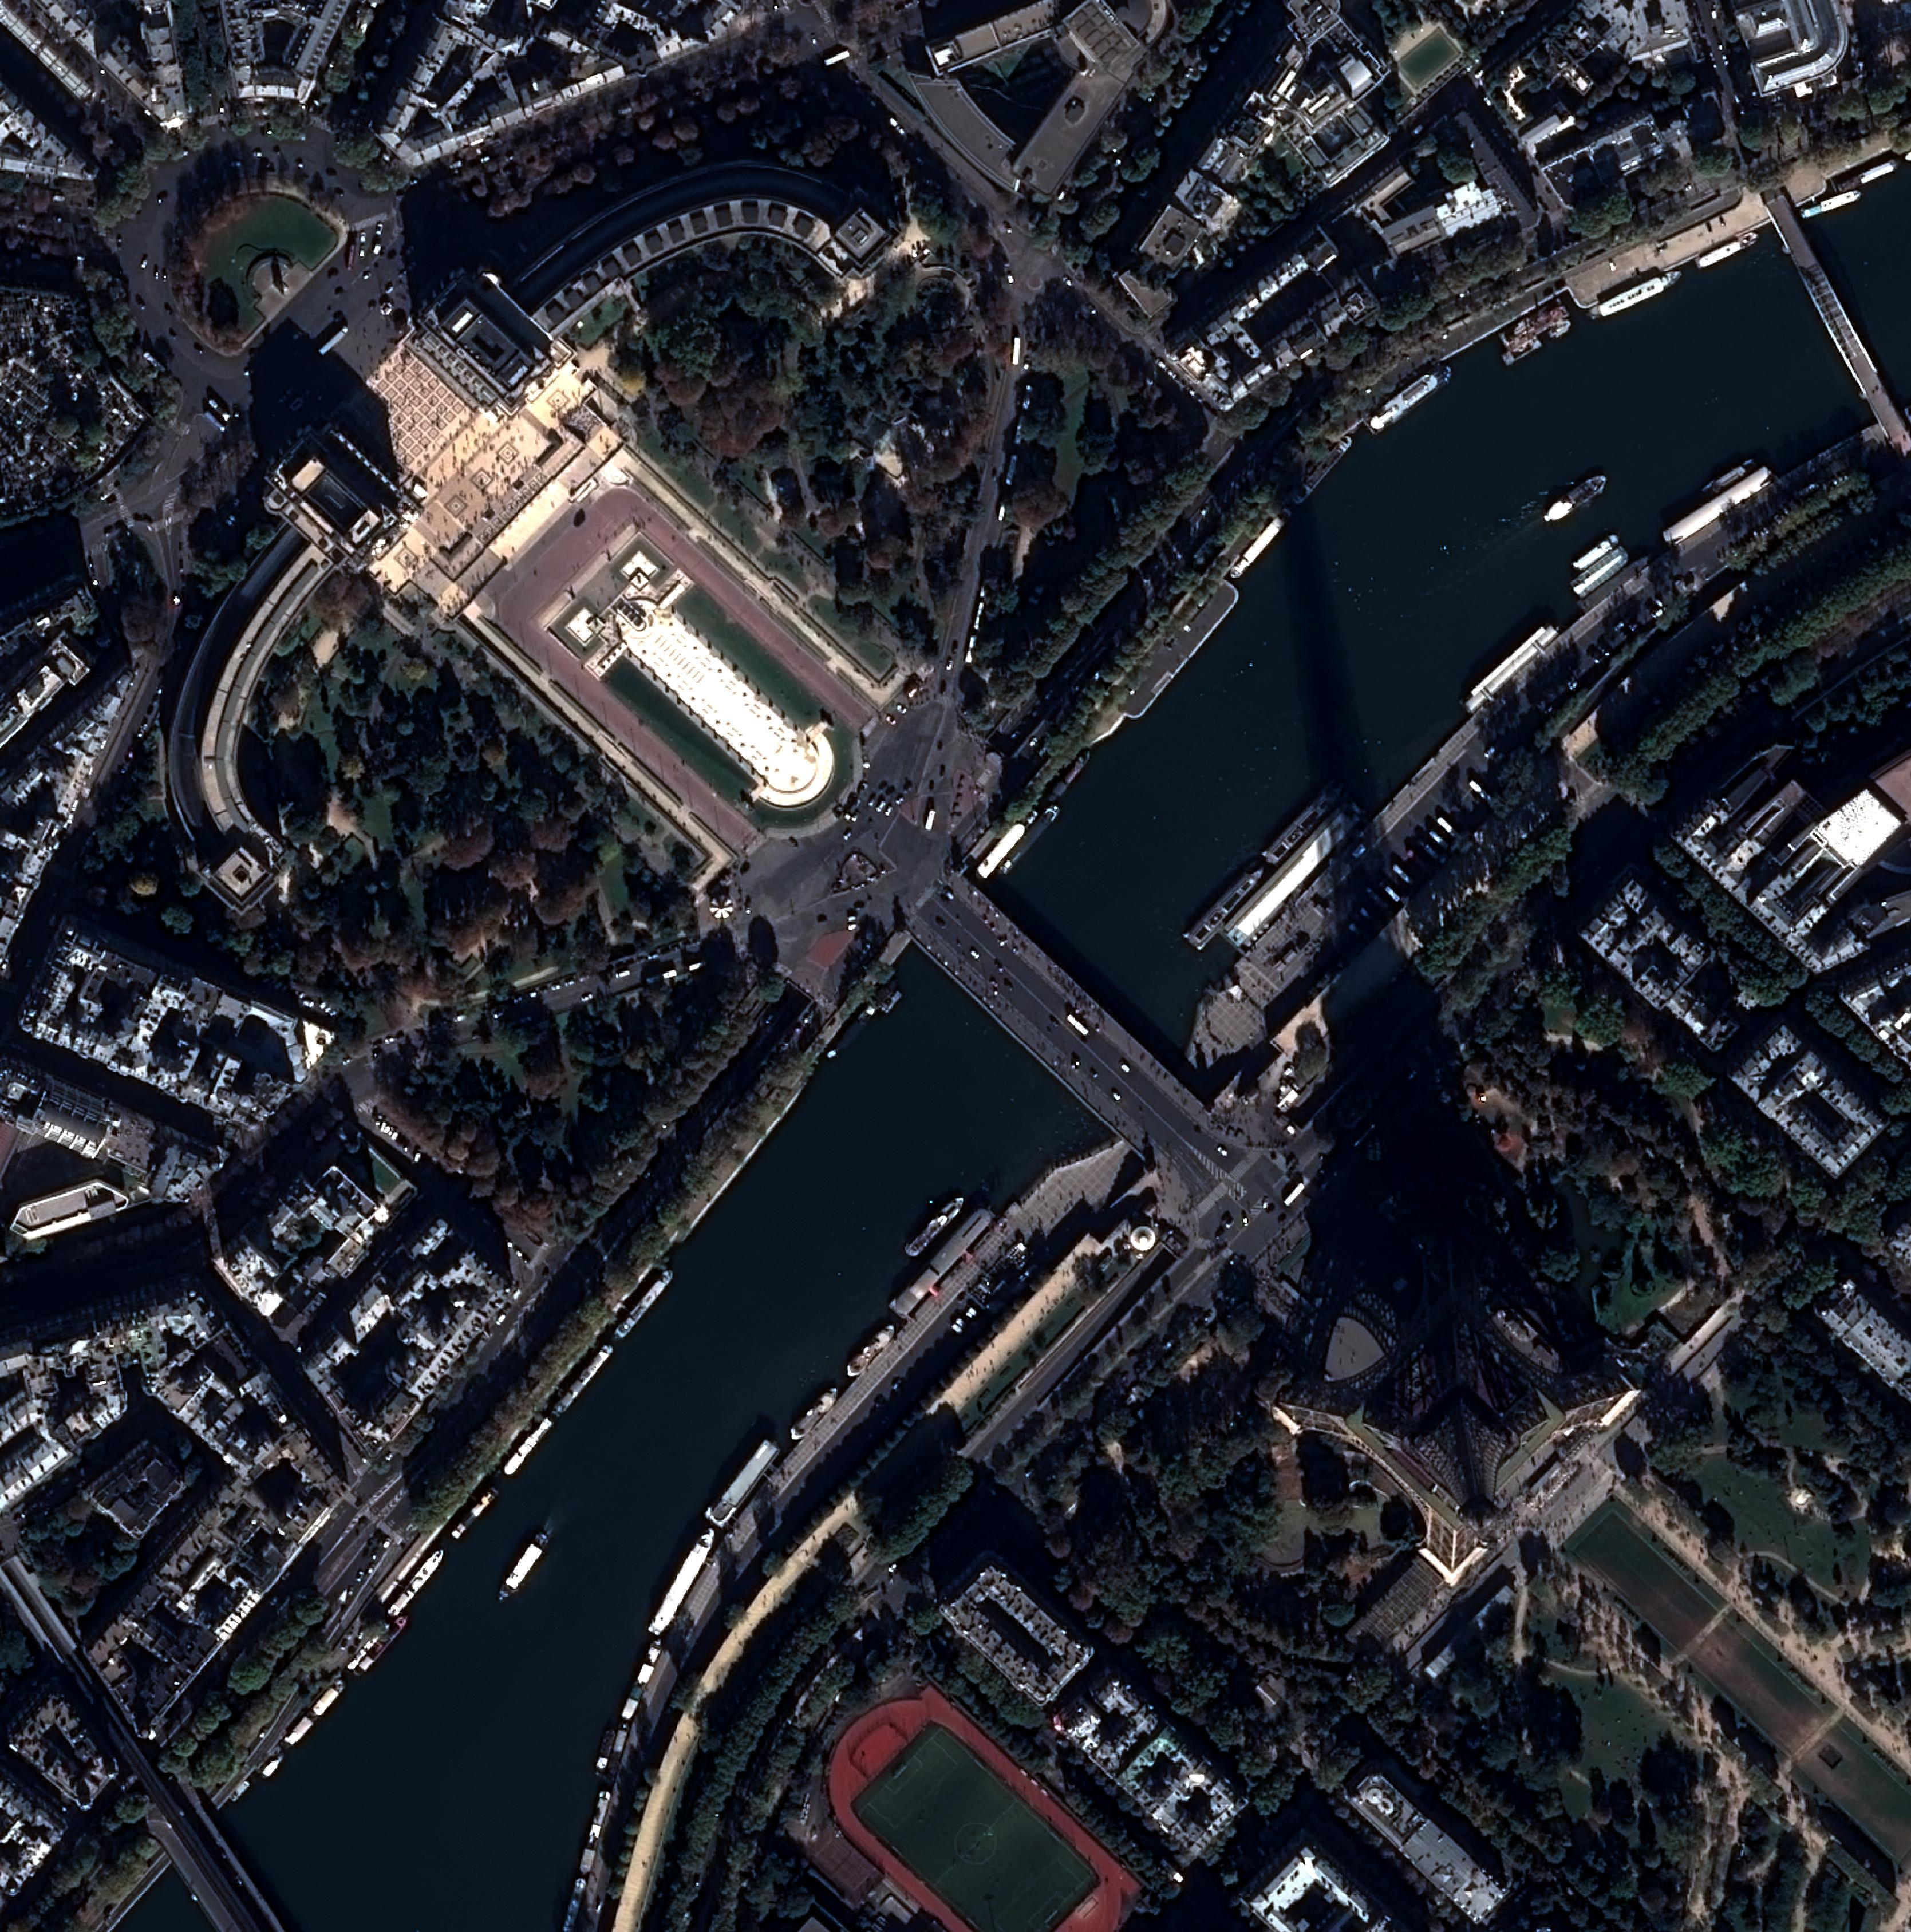
\includegraphics[height=6cm]{Images/Chap_1/Paris_003.jpeg}
        \caption{$14/10/2017$ $11:03:003$}
        \label{fig:Pleiade_over_Paris_a}
    \end{subfigure}\hfill
    \begin{subfigure}[t]{0.5\linewidth}
        \centering
        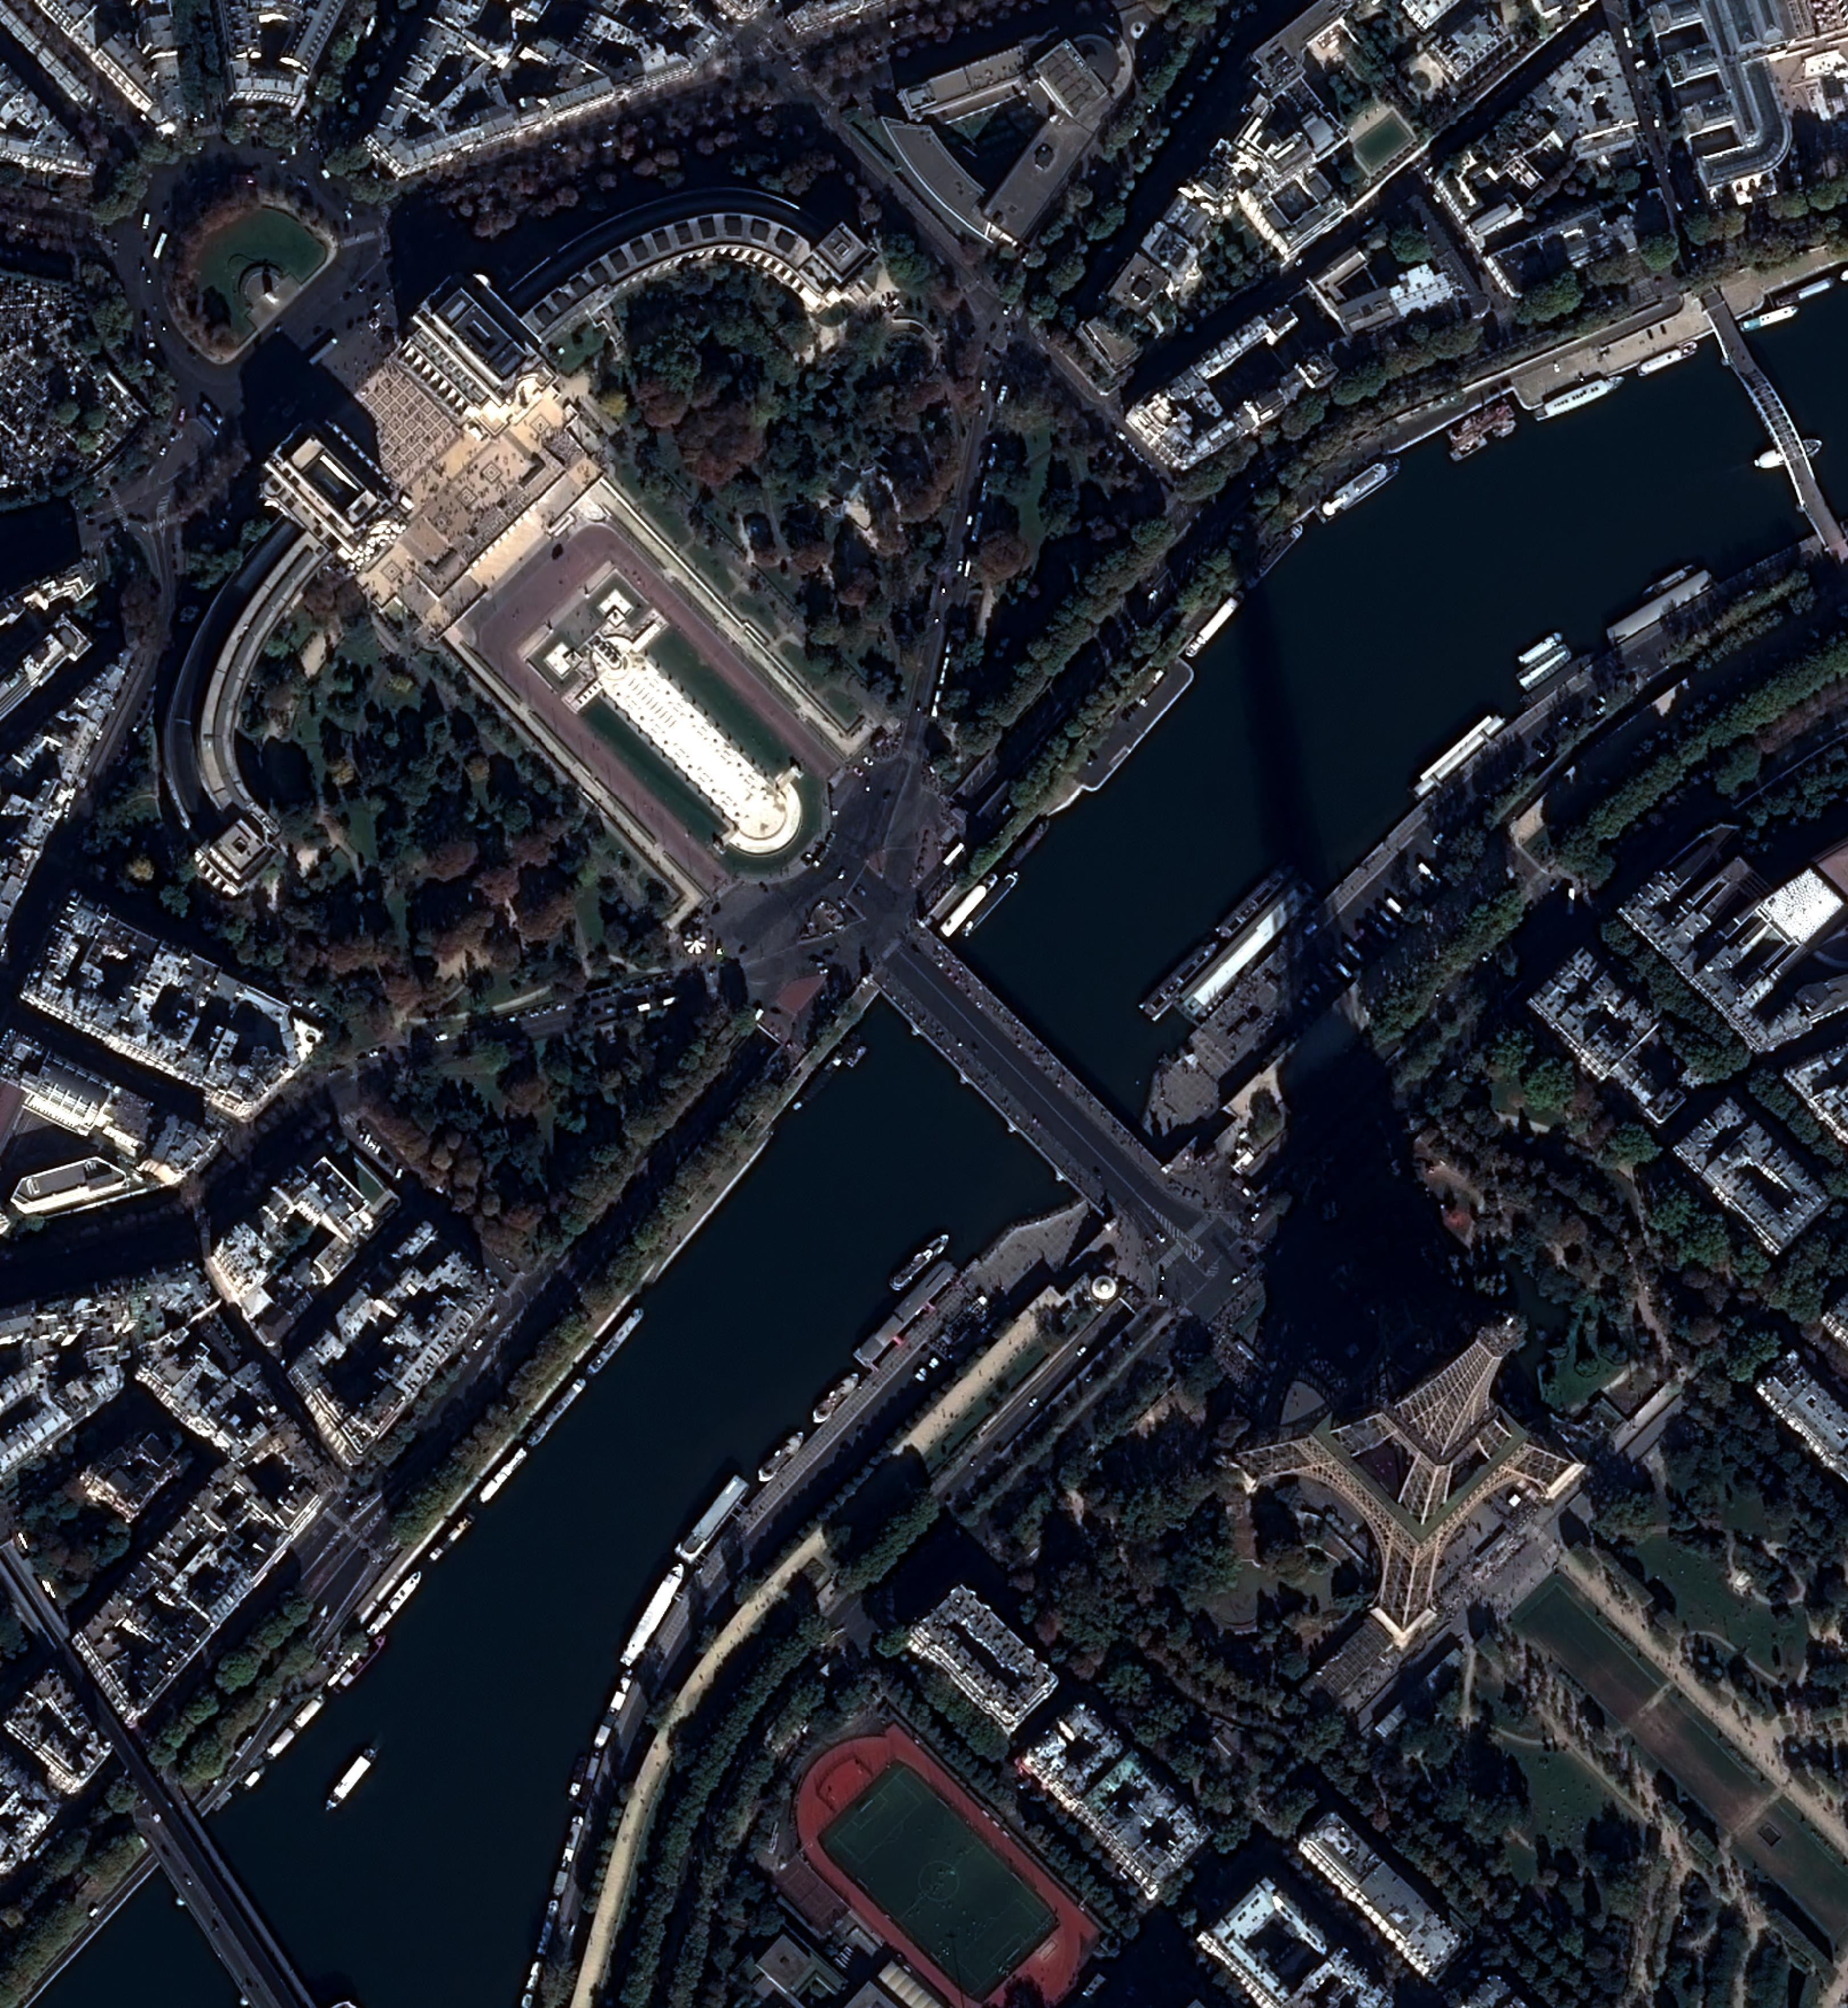
\includegraphics[height=6cm]{Images/Chap_1/Paris_403.jpeg}
        \caption{$14/10/2017$ $11:03:403$}
        \label{fig:Pleiade_over_Paris_b}
    \end{subfigure}
    \caption{Pansharpened Pléiades stereo images over Paris at $0.5$m of resolution. Pléiades \copyright CNES 2017, Distribution AIRBUS DS}
    \label{fig:Pleiade_over_Paris}
\end{figure}

In order to produce a worldwide \acrshort{dsm} with $1$m resolution by 2025, the \acrfull{cnes} is launching the \acrfull{co3d} mission \cite{melet_co3d_2020}. Composed of two pairs of low-cost satellites equipped with \acrshort{vhr} optical sensors, the mission will produce image in the \acrshort{rgb} and \acrshort{nir} spectrum at $0.5$m of resolution \cite{lebegue_co3d_2020}. The pairing of satellites allows for \textit{almost} simultaneous stereo image acquisition, cutting short the transient object problem (\ie objects moving/disappearing between stereo images). To be able to process the amount of data provided by the CO3D mission ($40\,000$ images a day, at $50cm$ resolution and covering a footprint of $7km\times5km$ \cite{melet_co3d_2020, lebegue_co3d_2020}), every step of the pipeline has been developed to be highly parallelizable\commanu{scalable ? to be scalable -> passer à l'échelle. plus large que juste le calcul parallèle qui est une facette de l'optim}. Different acquisition schemes can also be used, such as the video mode, or even the `diamond' geometry acquisition, which acquires a quadri-stereo over a couple of days. Depending on the relief of the terrain observed, the \acrshort{b/h} ratio will be between $0.2$ and $0.3$\commanue{Détaille un peu dans les paysages naturels, les satellites s'éloignent pour augmenter le B/H et dans les zones urbaines ils se rapprochent pour limiter les occlusions}. In parallel with image quality specifications, the CO3D products need to abide to a height accuracy of $1$m on low slopes \comloic{à vérifier je crois que c'est 1m en relatif à CE90. En absolu je ne sais plus}. Another requirement, which is particularly relevant in the context of this thesis, is the production of a performance map supporting the output \acrshort{dsm}. Investigating sources and propagation of the uncertainty inside a 3D stereo pipeline can be beneficial for this performance map requirement\commanue{Je dirais plutôt In addition, the project plans to produce a performance map supporting the output DSM. Therefore, investigating sources and propagation of the uncertainty inside a 3D stereo pipeline is essential for the implementation of this performance map.}\commanu{idem que manue avec juste investigating uncertainty inside a 3D stereo... serait plus direct, tu parles des sources et propagation ailleurs, pas besoin de compliquer la phrase}. 
\todoroman{Dire qu'on est partis du besoin utilisateur pour faire notre méthode et pas l'inverse.}\commanue{Effectivement tu peux expliquer que pour répondre à ce besoin de créer une carte de performance, il existe plusieusr approches. On pourrait faire comme ce qui est fait dans les autres produits (attention c'est à vérifier sur les sites de l'IGN et du DEM coppernicus par ex) il y a une carte qui indiquent une classe de confiance dans le résultat. C'est souvent un masque avec des flags de qualité qui permet de dire si le traitement c'est bien passé ou non. Toi tu as choisi une optique différente en demandant aux utilisateurs quelle information d'incertitude ils attendaient. Et ensuite blabla tu connais l'histoire comme moi.}\commanu{+1}
\todoroman{Parler de Maxar avec les Worldview ?}\commanu{tu peux juste citer mais pas obligé, tu t'en sers pas...}

\todoroman{Schema de la mission CO3D. Type of sensor, push-broom vs raster for CO3D. Pour info c'est une matrice de Bayer}

\begin{remark}
    When an image is acquired both in panchromatic and RGB mode, it is possible to leverage the high resolution of the panchromatic image to improve that of the color image. This fusion technique is called \textit{pansharpening} \cite{loncan_hyperspectral_2015}. We use this technique for clarity in figures and other illustrations of this thesis. It is important to remember that the processed images are the panchromatic images, and not the pansharpened ones which are only used for the final visualization.\commanue{Pour CO3D c'est un peu différent car matrice de Bayer.}
\end{remark} 
\commanu{je sais pas si besoin de cette remarque panchro RGB ici, peut etre quand tu l'utilises plus tard ?, tu verras à la relecture finale. et oui attention différent sur CO3D}

\section{Sensors and Geolocation}\label{sec:sensors_rpc}\commanue{là la transition avec cette partie est plus complexe. Peut-être que je mettrais les éléménts concernant les différents capteurs dans le paragraphe précédent lorsque tu présentes les satellites. Et je déplacerais la partie géoloc dans le pipeline par ex dans une section au début (que tu n'as pas qui explique le niveau de produit que l'on utilise pour faire de la 3D donc image en géométrie capteur avec un modèle de prise de vue où tu peux expliquer que dans ton cas c'est un RPC car le comprimis entre précision et facilité d'utilisation est acceptable.)}
Different types of sensors can be used to acquire satellite images. Below is detailed a (non-exhaustive) list of sensors of interest \cite{cnes_imagerie_2008}

\textbf{CCD matrix sensor}. CDD are classical sensors used, for instance, in current digital cameras. They possess multiple advantages, such as good geometrical quality as all pixels are acquired simultaneously, or the possibility to perform many acquisitions with various angles possible. However, CCD sensors with small pixel sizes are technologically difficult to built. Augmenting the number of pixels complicates the shutter function\commanue{et ça prend de la place. Alors que qq lignes pour un push-broom c'est plus compact}, and requires more radiometric calibration as one pixel equals one sensor\commanue{là je ne suis pas sure de comprendre la remarque}. It is also more complex to acquire long segments of an image \commanue{il faut peut-être expliqué que le satllite est toujours en mouvement donc là tu dois faire en sorte de ralentir (façon de parler car en réalité le satellite qui pivote pour fixer la zone à aquérir suffisamment longtemps pour avoir assez de petits photons)}. CO3D satellites will use this technology\commanue{moi je mettrais cela dans la description de CO3D}.

\textbf{Push-broom sensor}. Those image sensors are only composed of a single cell row, acquiring simultaneously radiometric information alongside a line perpendicular to the direction of the satellite\commanue{peut-être précise que dans ce cas on utilise la vitesse de défilement du satellite}. As only one line of cells is needed, push-broom sensors are simple systems which can capture images continuously, while guarantying good geometrical quality along the rows of the images. A variation of those sensors are TDI sensors (Time Delay Integration). Those sensors function as a push-broom except that each row has the ability to transfer its photon charges to the next row. This allows to capture signals over a longer period of time,  thus reducing the signal-to-noise ratio. Harder to produce, TDI sensors also require a precise control of the satellite so that observed objects stay within a column of the TDI sensor. They are used in Pléiades satellites for instance\commanue{je remonterais cette partie quand tu décris les capteurs HR actuellement en vol.}.

\todoroman{Regarder "Developement and Implementation of Rational Polynomial Coefficient Algorithms for Georeferencing Cartosat-1 Data", et "Metric Information Extraction from Spot Images and the Role of Polynomial Mapping Functions" de Baltsavias et Stallmann}
\commanue{Comme mentionner précédement je mettrais cela plus loin quand tu décris le pipeline CARS. Je ferais une section dédiée sur le fait que CARS prend en entrée une image en géométrie capteur avec un modèle de prise de vue. Si tu veux tu peux préciser qu'il s'agit d'une image où les bandes sont recalées entre elles. Tu peux expliquer à quoi correspond un pixel. On est pas sur une image géoréférence comme on pourrait utiliser dans un SIG. Et ensuite c'est parti pour le modèle de prise de vue... }\commanu{d'accord avec ca}A crucial part of satellite imagery is the ability to perform georeferencement, or georegistratation, of every pixel, \ie, locate their coordinates in an Earth system of coordinates such as latitude and longitude. Physical models possess high geolocation accuracy, but are sensor-specific and are computationally complex. For stereo reconstruction,  generalized sensor models are preferred. Specifically, we will focus on \acrfull{rpc} \cite{grodecki_ikonos_2001} used by the \acrshort{co3d} and Pléiades satellites, and provided alongside images. Sometimes called Polynomial Mapping Functions \cite{baltsavias_metric_1992} or Rational Function Models \cite{tao_comprehensive_2001}, \acrshort{rpc} are functions allowing to transform a pixel's ground location $(X,Y,Z)$ into its image coordinates $(row, col)$. \acrshort{rpc} encode lines of sight of the satellite, \ie the line joining the center of the sensor's cell to the ground and going through the optical center of the sensor. To improve numerical stability and minimize computation errors, the image coordinates and ground coordinates are normalized between $-1$ and $1$, using their scale factors $SF$ and mean values:
\begin{eqnarray*}
    SF_X &=& \max(X_\mathrm{max}-\overline{X},~\overline{X}-X_\mathrm{min})\\
    \Tilde{X}&=&\frac{X-\overline{X}}{SF_X}
\end{eqnarray*}
The same processed is applied to $Y,Z,row$ and $col$. To avoid heavy notation in this section, we will refer to every normalized coordinate using their non-normalized symbol.

\begin{figure}
    \centering
    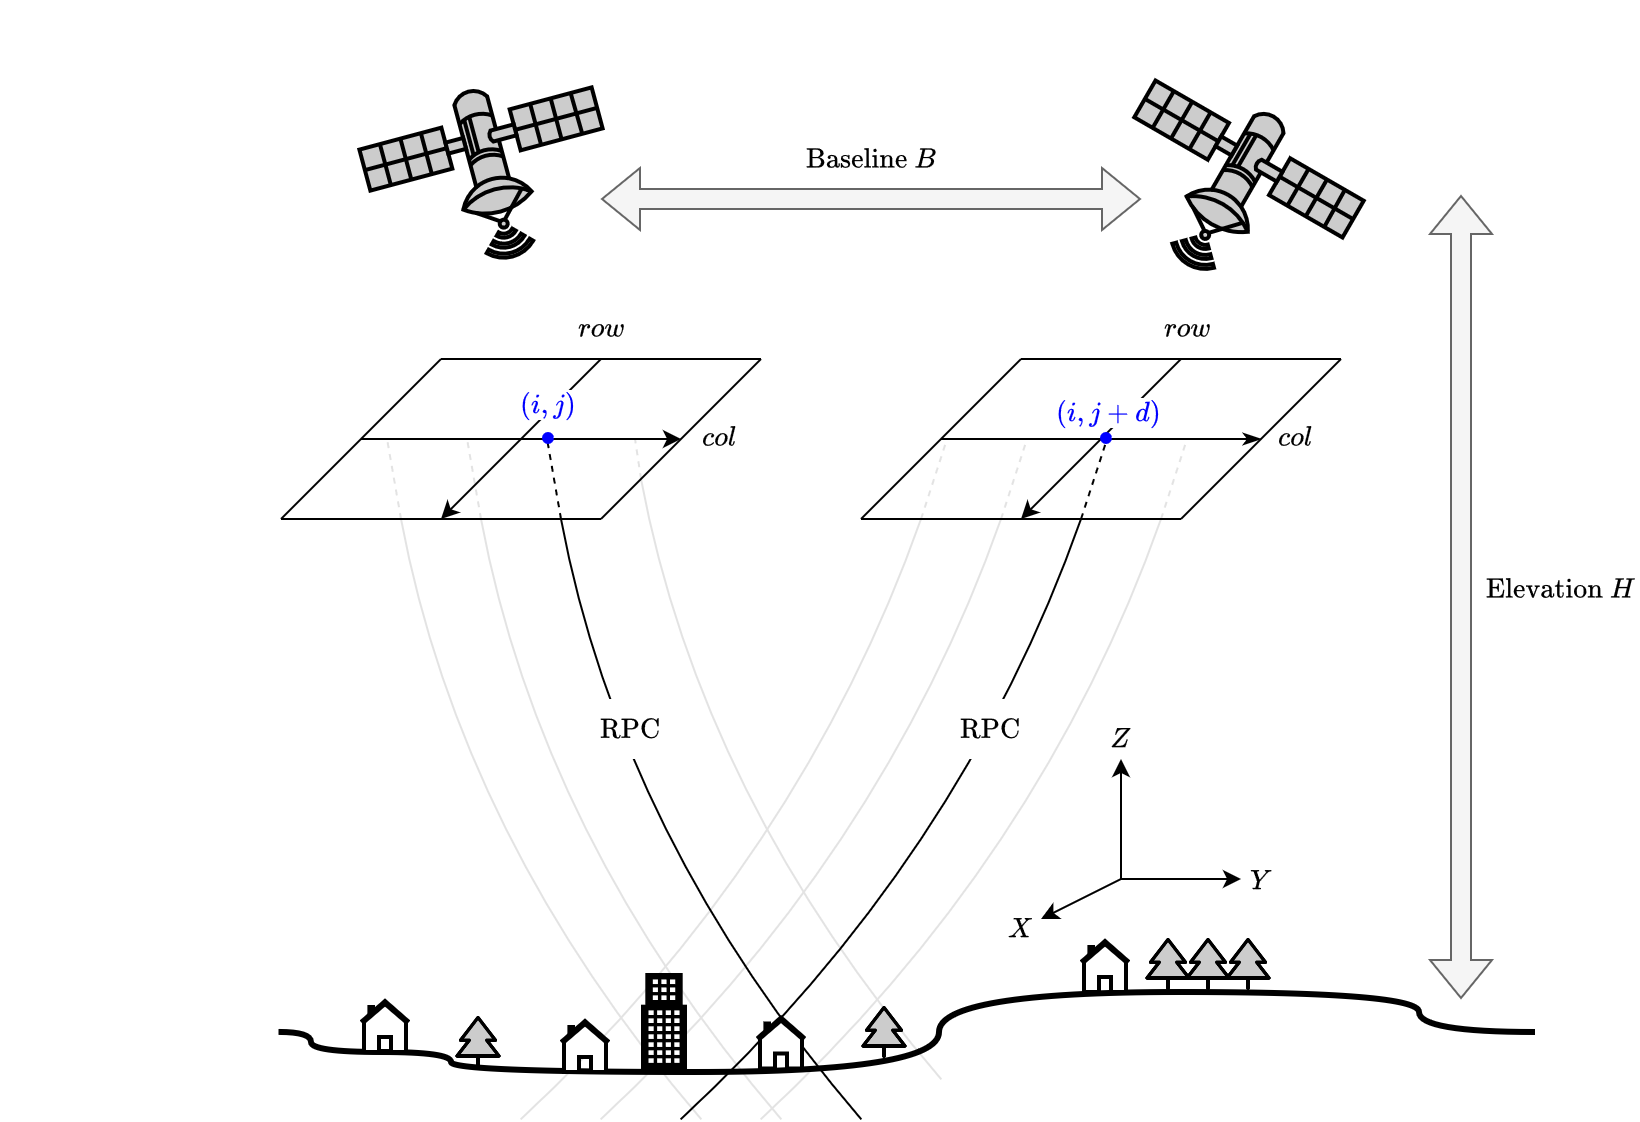
\includegraphics[width=0.8\linewidth]{Images/Chap_1/RPC.png}
    \caption{Triangulation of the position of a point using RPC models}
    \label{fig:RPC}
\end{figure}

Formally, \acrshort{rpc} are defined as rational fractions of polynomials:  
\begin{eqnarray}
    \RPC:\mathbb{R}^3 &\rightarrow&\mathbb{R}^2\nonumber\\
    (X,Y,Z) 	&\mapsto& \left(\frac{Num_{row}(X,Y,Z)}{Den_{row}(X,Y,Z)}, \frac{Num_{col}(X,Y,Z)}{Den_{col}(X,Y,Z)}\right)\nonumber\\
    &\mapsto&(row,col)\label{eq:rpc}
\end{eqnarray}
where $Num_{row},~Den_{row},~Num_{col}$ and $Den_{col}$ are the numerators and denominators for rows and columns respectively, expressed as polynomials with a maximum order of $3$:
\begin{eqnarray*}
    Num_{row}(X,Y,Z) &=& \sum_{i=0}^3~\sum_{j=0}^{3-i}~\sum_{k=0}^{3-i-j}a_{ijk}X^iY^jZ^k\\
    &=& a_{000} + a_{100} X + a_{010} Y + a_{001} Z + a_{110} XY + a_{101} XZ \\
    &&+ a_{011} YZ + a_{200} X^2 + a_{020} Y^2 + a_{002} Z^2 + a_{111} XYZ \\
    && + a_{210} X^2Y + a_{201} X^2Z + a_{120} XY^2 + a_{102} XZ^2\\
    && + a_{021} Y^2Z + a_{012} YZ^2 + a_{300} X^3 + a_{030} Y^3 + a_{003} Z^3
\end{eqnarray*}
$Den_{row},~Num_{col}$ and $Den_{col}$ respectively possess different coefficients $a_{ijk}$. The order or indexing of $a_{ijk}$ may differ in the literature. For instance, they can be numbered from $0$ to $19$ or $1$ to $20$, and do not refer to the same indeterminate. \acrshort{rpc} are computed using reference ground control points.\commanue{Discute avec Daniel mais tu peux effectivement utiliser des poinst de contrôle pour fitter les ceoff mais dans le cas des segments-sols, ils utilisent le modèle physique et ensuite ils fittent sur ce modèle un modèle RPC pour les utilisateurs normaux.}

It has been showed in \cite{baltsavias_metric_1992} that RPC are well suited to be used for ortho-rectification and stereophotogrammetry, as they possess good accuracy and are computationally fast. For stereo photogrammetry, it is ofter required to use the inverse \acrshort{rpc} model. As \acrshort{rpc} encode a line of sight given an image coordinate, the use of an additional elevation coordinate is required to move from the image space to the object space (\ie to go from a 2D space to a 3D space). It can be a geoid modelling the Earth's surface, or a \acrshort{dsm} with higher resolution. Knowing the true elevation $Z$ of a pixel, we define the inverse model as:
\begin{eqnarray}
    \RPC^{-1}:\mathbb{R}^3 &\rightarrow&\mathbb{R}^3\nonumber\\
    (row, col, Z) 	&\mapsto& (X,Y,Z) \label{eq:inverse_rpc}
\end{eqnarray}

An illustration on how RPC are used in stereo-photogrammetry is presented in \Cref{fig:RPC}. \commanu{c'est dommage de pas l'utiliser pour l'étape de triangulation. Ici, l'exemple le plus direct serait juste une loc sur ellipsoid ou DEM, ca evite au lecteur de penser autre chose (exemple image page accueil https://shareloc.readthedocs.io/)}

\section{Structure of the Stereophotogrammetry Pipeline}\label{sec:classical_stero_pipeline}
This section dives more into details of the inner workings of stereophotogrammetry\commanu{soit cohérent tout le long, 1 mot, 2 mots? pas pareil partout (dans l'intro t'as mis 2 mots)}, and presents the stereo pipeline mainly considered in this thesis. Photogrammetry is the science of deducing information from photographic images\commanu{ref ? un livre référence par exemple}. A sub domain of photogrammetry is stereophotogrammetry, which specifically consists in deducing 3D information from multiple photographic images. Although multiple stereophotogrammetry setups can be achieved, for instance using structured light \cite{scharstein_high-accuracy_2003} or different wavelength \cite{geng_rainbow_1996}, we focus here on the pipelines designed for processing satellite images, which are used and studied in this thesis. 

The main idea of stereophotogrammetry for satellite images and other 3D pipelines is to identify the parallax of objects between multiple images, and to deduce the distance between the object and the sensors from this displacement\commanue{Tu as le droit de mettre des schémas en plus tu risques d'en avoir besoin pour ta prez}. When expressed in pixels, the displacement is called disparity\commanue{si tu as un schéma plus loin mets une ref, sinon fait un schéma. C'est important que les termes que tu vas utiliser un nombre incalculable de fois par la suite soient bien définis}. To determine this disparity, the images must first be corrected from atmospheric effects (small clouds, aerosols, \etc) to go from top-of-the-atmosphere radiance to the actual light that illuminates the Earth surface \cite{hagolle_maja_2017}, called reflectance \comloic{je ne sais pas à quel point c'est vrai dans le cas de CO3D. Les acquisitions sont synchrones et le B/H petit. Je serai supris que en TOA les résultats soient très différents mais peut être. En tout cas je n'ai pas en tête de travaux qui le montrent.}\commanue{Alors si CO3D respecte le process standard la correction atmo c'est au niveau 2A donc tes images sont déjà projetées au sol donc on ne fait pas de 3D avec elles. Les images pour faire de la 3D c'est en général ce qu'on appelle de niveau 1B (correction radio et géo (recalage et modèle géométrique). A partir de 1C on projette au sol. Mais à vérifier avec David si CO3D utilise les niveaux de produits standards}. Many stereo setups\commanue{Alors là tu t'éloignes du satellite, je ne sais pas s'il ne faut pas le préciser. Ici quand tu parles de setups c'est les autres applications utilisant la 3D comme les voitures autonomes, les rovers sur Mars que tu as en tête} align their cameras in such a way that objects only move horizontally between images \cite{geiger_are_2012, scharstein_high-resolution_2014, keselman_intel_2017}. This allows to restrict the search space for pixel matches to a single row instead of the whole image. In a way, most people's eyes also present this alignment\commanue{je suis d'accord avec l'analogie mais la transition avec in a way c'est bizarre.}. When operating satellites, it is more complex to ensure that the sensors disposition will stay consistent\commanue{peut-être le tourner différemment, comme tu le mentionnes, habituellement dans les autres applications qui utilisent de la stéréo, les caméras sont montées de telle sorte à être dans la géométrie. Tu fais du principe d'acquisition satellite (qui défile) on n'est pas dans ce cas. C'est pas que c'est plus complexe. C'est que le mode d'acquisition ne le permet pas.}, thus requiring some pre-processing step to rectify images and ensuring that the displacement of an object only occurs horizontally (see \Cref{sec:epipolar_geometry}). Then matching pixels are determined by computing their disparity in a step called stereo matching presented in \Cref{sec:stereo_matching}\commanue{je suis en train de me dire que ce que tu racontes est très liée à la géométrie épipolaire. Mais que dans les faits les pipelines satellites font parfois le choix de reprojeter l'image de droite dans la géométrie de l'image de gauche donc corrélateur 2D car la mise en géométrie épipolaire est complexe. Donc peut-être que dans toute cette partie l'intérêt de la géométrie épipolaire doit être gardé pour plus tard et de rester haut niveau pour l'instant en disant seulement que l'étape consiste à trouver les pixels homologues entre deux images ou même pas car dans cette section, tu te limites à parler d'objets et non pas de pixels}\commanu{je suis d'accord, je ferais plus simple et ferait en 2 fois}. The 3D coordinates of the corresponding object are determined by computing the intersection between matching pixels' lines of sight (or best approximation if they do not strictly intersect). This results in a point cloud, where each point correspond to a match of two pixels\commanue{là on repart sur la notion de pixels donc soit tout ton paragraphe raisonne avec des objets dans les images soit tu parles de pixels dans les images. Mais si tu passes de l'un à l'autre c'est perturbant car les deux notions ne sont pas interchangeables}. The point cloud can be processed to remove outliers, and is then projected into a regular grid to obtain the desired \acrshort{dsm}. The following section dives more into details for the specific case of the CARS stereo pipeline\commanue{bah en fait non, dans la suite tu repars sur les pipelines existants. Donc je mettrais un peu d'ordre. Tu as fait un paragraphe très générique sur ce qu'est un pipeline 3D. Ce que tu as raconté ici, s'applique à tous, ça tombe bien c'est l'intro. Ensuite nouvelle section tu mentionnes les pipelines existants, tu peux fortement t'inspirer de ce que j'avais écrit pour ISPRS pour CARS. Tu auras peut-être besoin de la géometrie épipolaire. Et après tu enchaines sur CARS.}\commanu{en effet, mieux avec 1 général 2 pipeline existant 3 le notre cars, ca cleanera le meme feeling que manue entre ses deux sous sections}.

\subsection{Structure of the Stereo Pipeline}
Several stereo pipelines processing satellite images exist in the literature. We can think of NASA's \textit{ASP} \cite{shean_automated_2016}, IGN's \textit{MicMac} \cite{rupnik_micmac_2017}, Centre Borelli's \textit{s2p} \cite{franchis_automatic_2014}, DLR's \textit{CATENA} \cite{kraus_fully_2013}, Ohio State University's \textit{RSP} and \textit{SETSM} \cite{qin_rpc_2016, noh_surface_2017}\todoroman{Regarder "Metric Evaluation Pipeline for 3D Modeling of Urban Scenes" pour des comparaisons}. All those pipelines roughly possess the same structure, \ie pre-processing, images resampling in a convenient geometry for pixel matching, dense matching, triangulation and rasterization. Variations in those pipelines concern the different preprocessing steps (bundle adjustment, histogram equalization), the type of geometry used, the dense matching algorithms available \etc\commanue{Donc pour un chapitre de thèse va falloir plus détailler, je suis sure que j'ai mis plus d'info dans la publi de CARS ;) Il faudrait ajouter par rapport à ce que j'avais moi, c'est si certains pipelines gèrent ou non les incertitudes. Je n'avais pas regardé ce point à l'époque. Sans parler d'incertitudes, tu as peut-être a minima des flags qualité qui permettent au moins de dire ce résultat-là on regarde même pas}\commanu{et du coup, je découperais: une partie à part état de l'art des satellite stereo pipeline + une partie dédiée sur cars, revoir ta structure pour aider le lecteur} We will focus on the CARS pipeline used in this thesis, developed by CNES \cite{michel_new_2020}. A schematic of the different steps of the pipeline are presented in \Cref{fig:cars_pipeline}.
\todoroman{Insister sur le fait que CARS est tout automatique, y compris sur les cartes de performances à grande echelle. A voir avec Sylvia comment les DEM de l'IGN ont une carte de perf, et si oui si elle est pas manuelle}

\begin{figure}
    \centering
    \includegraphics[width=\linewidth]{Images/Chap_1/CARS_pipeline_detailed.png}
    \caption{Different steps of the CARS pipeline}
    \label{fig:cars_pipeline}
\end{figure}
The CARS pipeline works with grayscale images, but colored images (for instance pansharpened image) can be provided alongside the grayscale image\commanue{alors petite précision, Pandora ne fait de la corrélation que sur une seule bande. Donc CARS en général utilise les images PAN car plus résolues et ensuite complète sa sortie avec des infos issues du RGB. Donc je dirais plutôt que CARS (à cause de l'étape de corrélation) travaille majoritairement en mono-bande. Après si on envisage des étapes où on se sert du RGB par exemple pour faire de la classif ou pour filtrer, on pourrait avoir une plus grande utilisation de l'information provenant de plusieurs bandes}\commanu{je sais pas si c'est central en effet. a la lecture, ca donne l'impression que c'est important alors que c'est un peu annexe: ici tu présentes surtout les grandes étapes et les grandes lignes de fonctionnement du pipeline. La color peut etre un sujet intéressant mais annexe à ta problématique, attention digression comme vu par manue}. The grayscale pixels will be used in the pipeline\commanue{car les PAN sont plus résolues pour les images Pléiades. Pour CO3D on prendrait la bande verte car 2 fois plus de pixels}, but the colorimetric information will be kept until the final DSM, thus providing an ortho-rectified image\commanue{C'est pas faux mais il faut que tu fasses attention à toutes ces petites remarques que tu ajoutes et qui peuvent perdre le lecteur. As-tu besoin de parler les images orto RGB? Si oui, vraiment maintenant ou peut-être au moment de la rasterisation}.\commanue{Donc là voir remarque précédente, mais je mettrais ici clairement ce que c'est que les inputs de CARS : image en géométrie capteur mono-bande avec un modèle de prise de vue.}

\subsection{Resampling in Epipolar Geometry}\label{sec:epipolar_geometry}
The first step of the CARS pipeline is to resample the stereo acquisitions into a convenient geometry to carry out the dense matching\commanue{alors dans l'intro de cette section (qui es utile pour poser les termes), tu n'as jamais dis dense matching. Tu as juste parlé de matching (j'ai vérifié) donc dis juste matching entre les pixels. Tu expliqueras le terme dense dans l'étape de matching à proprement parlé}. This geometry is the epipolar geometry \cite{cnes_imagerie_2008}, which is constructed so that each line of an image follow the movement of the satellite, \ie the objects move only horizontally between the reference and secondary stereo images. This will\comloic{pourquoi will?} greatly facilitates the dense matching\commanue{juste matching} as the search space for a match is only limited to a one dimensional space instead of a two dimensional space around the pixel\comloic{la fin de la phrase est peut être pas utile}. A first approximation\commanue{pourquoi first approximation?} of the epipolar geometry can be computed using the respective geolocation models of both images $\RPC_1$ and $\RPC_2$\comloic{je suis peut être passé trop vite il me semble pas encore avoir croisé les termes RPC, ça vaut le coup d'en toucher un mot}. Indeed, given the altitude $Z$ of the object represented by pixel $(row_1, ~col_1)$ in the reference image, then\comloic{then pas utile} we can deduce its ground location $(X, ~Y, ~Z)$ using $\RPC_1^{-1}$. The position in the secondary image of those coordinates\comloic{là on ne sait pas trop si tu parles de la représentation du pixel (row,col) il y a deux phrases ou de la groud location} can then be retrieved using $\RPC_2$. In short, we found the secondary coordinates $(row_2,~col_2)$ of a pixel $(row_1,~col_1)$ in the reference image given an elevation $Z$\comloic{C'est pas limpide. Je vois comment ça marche dans ma cars mais là en te lisant je suis pas convaincu de l'ordre des opérations / explications}: 
\begin{equation}
    (row_2,~col_2) = \RPC_2\circ\RPC_1^{-1}(row_1, ~col_1, ~Z)\label{eq:epipolar_transfer}
\end{equation}
By varying the altitude in the range of considered elevations $[Z_{min},~Z_{max}]$, $\RPC_2\circ\RPC_1^{-1}$\comloic{tu peux la nommer f2->1 et préciser que c'est la fonction de colocalisation 2 vers 1} provides a characterization of the parallax between images. The lines described by $\RPC_2\circ\RPC_1^{-1}$ are thus the epipolar curves for the reference image\commanue{Tel que tu l'expliques, c'est plutôt la transformée d'une ligne de l'image de gauche par la composition des fonctions de RPC qui te donne la ligne épipolaire correspondante dans l'image de droite. Donc effectivement en faisant ça tu obtiens la ligne dans laquelle faire ta recherche. Mais il faudrait ajouter que c'est juste inutisable dans la pratique. On passerait son temps à faire des locs. Ce qu'on recherche c'est une transformation pour rééchantilloner les images}. Similarly, $\RPC_1\circ\RPC_2^{-1}$ provides the epipolar curves for the secondary. The range of considered elevations $[Z_{min},~Z_{max}]$ can be determined with a low resolution digital elevation model\commanue{pour faire une loc inverse tu as besoin d'une élévation donc n'importe quoi fait l'affaire.}. This is not constraining as a geoid of the Earth can be used, and there also exists open models such as the NASA's SRTM \cite{farr_shuttle_2007} ($30$m and $90$m of resolution between $-56\degree$ and $60\degree$ of latitude), or ESA's Copernicus DEM ($30$m and $90$m of resolution worldwide).  \todoroman{Parler aussi de la RGE Alti de l'IGN. regarder aussi s'ils ont un masque de perf}\commanue{Dans la suite tu repars sur le modèle pinhole. Donc cette partie sur le RPC on a l'impression que c'est pas fini. Peut-être commencé par parler du pinhole. C'est un modèle simple, c'est facile de calculer la transformée en géométrie épipolaire. Le souci c'est que le modèle pinhole n'est pas valide sur toute l'image mais localement. D'où l'utilisation du RPC mais les RPC ne permettent pas une formule analytique. Donc on passe par une grille de transformation. Et on utilise des compositions de fonctions de loc (et pour la fonction inverse on a besoin d'une hauteur).}

\begin{figure}
    \centering
    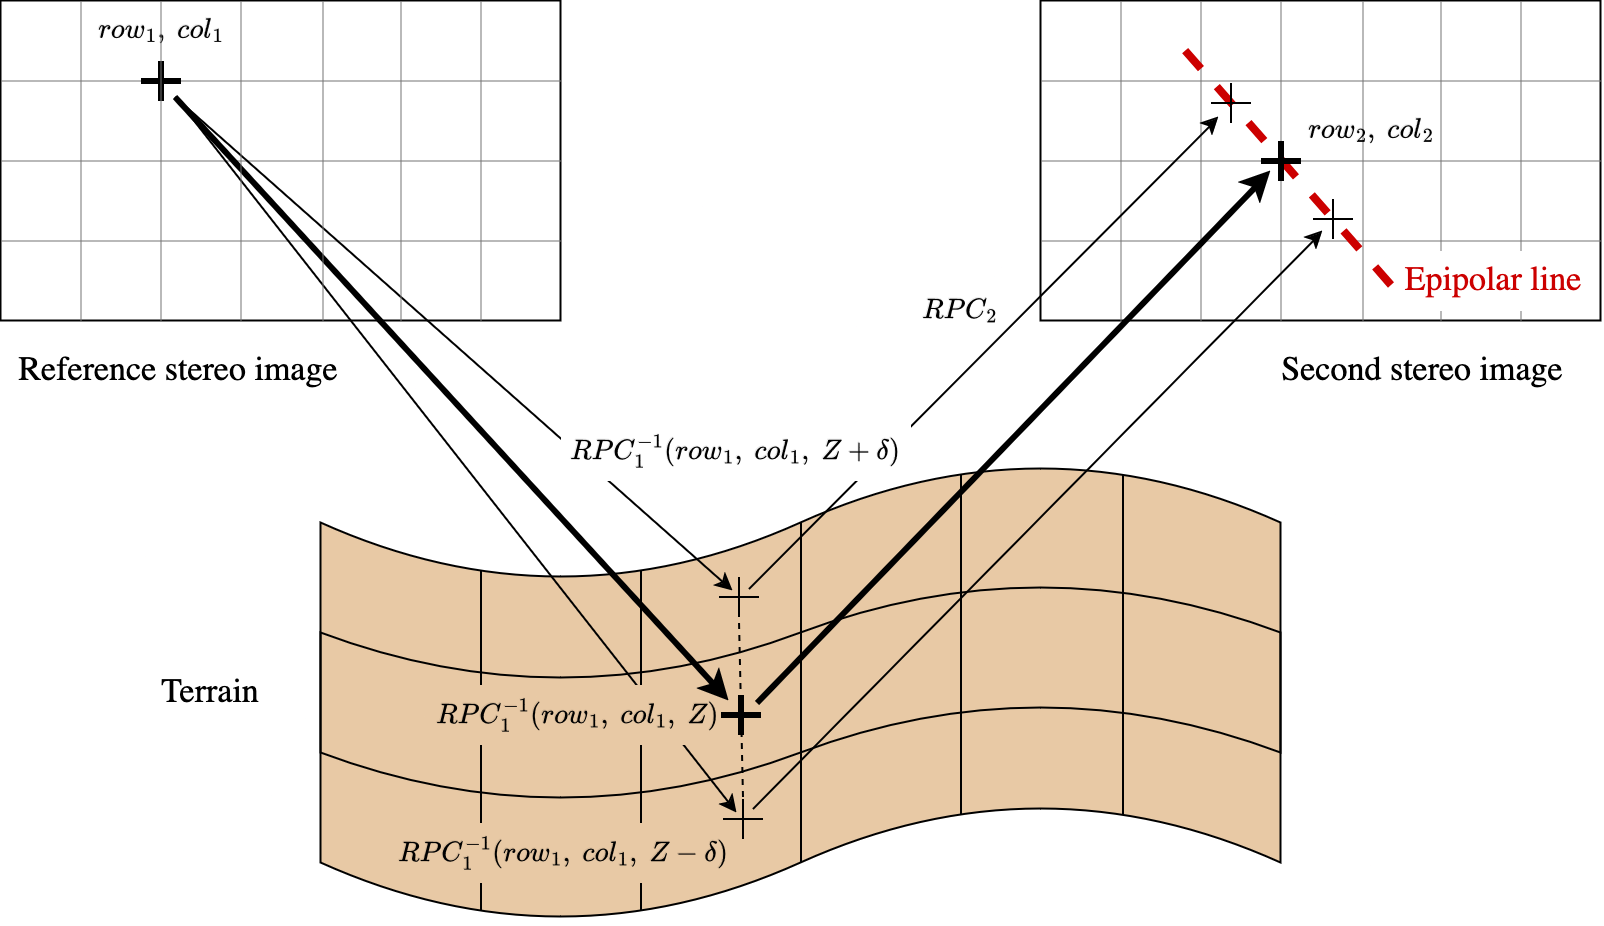
\includegraphics[width=\linewidth]{Images/Chap_1/epipolar_lines.png}
    \caption{Computation of an epipolar line for a pixel using small height variations}
    \label{fig:epipolar_lines}
\end{figure}

Captors using a pinhole camera model have a perfectly defined epipolar geometry, modeled by an affine transform \cite{hartley_multiple_2004}. This not true for push-broom sensors \cite{morgan_epipolar_2004}, but other models exist allowing to compute such a geometry \cite{oh_piecewise_2010, de_franchis_stereo-rectification_2014, koh_unified_2016, michel_new_2020}\commanue{Alors je mettrais la remarque en premier. Si on utilise un modèle simple pour décrire le modèle géométrique donc du pinhole c'est facile de faire le passage en géométrie épipolaire. Le pb c'est que le modèle pinhole n'est pas valide sur l'intégralité de l'image. Donc il faut l'appliquer par morceau, c'est ce que fait S2P. Résultat, tu as des effets de tuilages sur ton image. Ici on cherche une méthode pour passer en géométrie épipolaire en utilisant direct la précision du RPC. Alors tu cites la publi ISPRS de CARS mais justement on ne passe pas par du pinhole}\comloic{je rajouterai que ça va un poil vite. Quand tu dis qu'il existe d'autres modèles pour calculer la géométrie épipolaire tu passes un peu sous silence que ce sont des approximations, et justement la complexité dont on hérite avec des acquisitions de l'espace et des capteurs VHR principalement pushbroom, c'est qu'on ne peut pas exprimer la géométrie épipolaire de façon exacte sur l'ensemble du produit. Ensuite tu cites plusieurs papiers, il est important de noter ce qui distingue CARS des autres et notamment de la référence s2P (réf car IARPA winner tout ça tout ça). Dans s2p on a fait une approximation locale du modèle de caméra par un modèle type pinhole donc on peut réutiliser les algos de la computer vision à l'échelle d'une tuile sous réserve qu'elle soit petite. Dans CARS on cherche une représentation globale que l'on va exprimer par une grille de déformation qui fournit pour chaque point de la géométrie épipolaire sont équivalent dans la géométrie capteur.}. In the CARS pipeline, \cref{eq:epipolar_transfer} is evaluated with an elevation $Z$ extracted from the low resolution elevation model, and for small variations of altitude $Z\pm\delta$\commanue{alors je connais le principe mais là j'avoue que c'est pas clairement précédément tu as dit que tu pouvais avoir la ligne et là tu expliques que tu le fais localement. J'aurais tendance à renverser l'explication. Comme on ne peut pas avoir une trasformation analytique, on recherche une grille et voilà comme on évaluer chaque point de la grille.}. Those three points allow to compute the direction of epipolar lines for every pixel of both images as in \Cref{fig:epipolar_lines}\commanue{C'est un peu rapide. Comme on ne peut pas avoir une transformation en géométrie épiplaire qui peut s'écrire simplement via une transformation matricielle comme pour du pinhole. On décide d'exprimer la transformation par une grille que l'on peut prendre avec un pas assez large vu que les variations sont assez basse fréquence}. This method generates what is called an epipolar grid $g_{e1}$ joining every epipolar coordinate $(row_e, ~col_e)$ to its position in the reference image $(row_1, ~col_1)$:
\begin{align}\label{eq:epipolar_grid}
    g_{e1}(row_e, ~col_e) = (row_1, ~col_1)
\end{align}
A similar grid $g_{e2}$ is determined for the secondary image, which is actually computed jointly with $g_{e1}$. Those grids also use the low resolution elevation model\commanue{l'approche nécessite une altitude pour faire la loc inverse mais tu pourrais utiliser une altitude constante et la technique fonctionnerait. Si on utilise un DSM basse résolution c'est que cela permet de limiter l'intervalle de recherche.} to determine which altitude corresponds to a null disparity\commanue{Moi je tournerais plutôt la phrase qu'avec cette méthode par construction la disparité nulle correspond à l'altitude du DSM utilisé}\comloic{+1, c'est pas construction, tu peux amener ça de façon anecdotique, en gros c'est dans cette géométrie épipolaire là, puisqu'on pourrait en créer une autre, que la disparité nulle correspond à Z, où Z est censé être le Z dont tu parles plus haut et autour duquel tu ajoutes +/- delta, tu pourrais de Zcoarse ou Zdem. Enfin je veux dire, tu parles de Z en disant qu'il est extrait du low resolution elevation model mais on pourrait penser à un scalaire qui aurait au moins une occurence dans le low res elevation model, et peut être qu'il faudrait low res digital elevation model pour garder le lien avec DEM que tu présentes plus haut}. After the dense matching step, a disparity of $0$ would mean that the object has the same altitude than that of the low resolution elevation model. For more details on the way epipolar grids are computed, we refer to \cite{michel_new_2020}. Using those grids, it is possible to resample the reference and secondary images in their respective epipolar geometry. 

Because the geolocation models\comloic{c'est un termes que tu n'utilises que deux fois dans le manuscrit et je dirai qu'on pourrait l'introduire un peu mieux peut être pour ceux qui n'ont pas l'habitude de manipuler des images satellites. Peut être que dans le 1.3 le titre est trop vague, et le contenu fait un peu commercial plus que scientifique par moment. Je pense que tu pourrais y exposer plutôt des notations et des principes un peu originaux pour ceux qui découvrent l'image satellite mais sont qd mm intéressés par la thèse parce que par ailleurs ils font du stereo matching. Par exemple avant de parler des RPCs ou quoi faudrait introduire les systèmes de coordonées peut être. A la limite juste ECEF et UTM mais de quoi faire intervenir les notations X,Y, lon, lat, Z et h et les fixer pour le reste du manuscrit. Et ensuite seulement aborder les modèles géométriques et les RPCs et donc les loc directe et inverse. D'autre part à partir du 1.3 on parle souvent de DEM et d'intersecter un DEM du coup mais on parle pas du référentiel du DEM, en gros le Z du DEM il est par rapport à quoi ? faut faire intervenir géoide et ellipsoide je pense. Ou alors je vais trop loin mais là disons qu'on aborde tout ça très vite dans les premiers sous chapitre de cette section. Ensuite tu peux aborder les modèles de caméra utilisé dans le spatial un peu comme tu le fais mais sans le mélanger avec les RPCs, faudrait structurer avec un chapitre sur les syst de coord, un sur les modèles de caméra, un sur la géo d'acquisition en 3D qd même avec le b/h, avec le termes "nadir" peut être aussi, et ensuite les RPCs ou quoi)}  have a limited precision, there might be a misalignment left in the epipolar grids. To correct this error, a set of SIFT points \cite{lowe_distinctive_2004} is computed between the reference and secondary epipolar images. For every match, the difference between their rows is computed. The secondary epipolar grid is then corrected so that row differences are null on average. Once aligned epipolar grids have been obtained, stereo images can been resampled in epipolar geometry one last time so that \commanu{so that what ? à enlever ou finir la phrase}

\begin{remark}
    By computing the disparity for the set of SIFT points, it is possible to estimate the range of disparities to be considered in the dense matching step for a relatively low computation cost. We will see in \Cref{sec:triangulation} that there is an approximately\comloic{approximation?} allowing to simply convert disparities into an elevation using the $B/H$ ratio presented in \Cref{sec:stereo_matching}. Therefore, an approximation of the elevation of each SIFT match can easily be computed. A low resolution elevation model can then be derived from it, thus removing the need of an external model such as SRTM or Copernicus DEM.\commanue{Je ne suis pas sure que ça doit rester juste une remarque. MOn souci c'est qu'il y a plusieurs infos dans ta remarque. Premièrement les SIFT sont utilisés pour calculer l'intervalle de dispariaté,deuxième on peut convertir la disparité et troisièment on peut faire un DSM endogène. Donc la première partie de la remarque t'es surement utile. Le reste c'est à voir ou il faut faire plusiuers remarque.}\comloic{ouais c'est un paragraphe que tu pourrais avoir écrit la veille de la remise du manuscrit ça ;-) ça fait un peu, j'ai oublié deux trois choses qui rentrent pas dans le moule actuel donc je fais un patch. J'ai entendu dire que quand on fait un patch c'est un pb de conception si c'est pas un pb de temps ^^'}
\end{remark} 

Epipolar grids can also provide a good approximation of the disparity to altitude ratio $d_{alt}$ over the whole image, which can be used to determine the approximate $Z$ resolution of the DSM. It can also convert disparities into height as we will see in \Cref{sec:uncertainty_pandora}\commanue{Alors là je ne suis pas de comprendre le lien direct entre grille épipolaire et disparité}. 

\subsection{Stereo Matching}\label{sec:stereo_matching}
\subsubsection{Different Approaches}\commanu{pas sur que tu aies besoin de ce titre de soussoussection, j'enleverais}
Dense matching\commanue{je pense qu'il faut que tu prennes une phrase pour expliquer pour quoi on parle de dense matching. C'est assez typique de la télédétection où on fait du matching sparse pour recaler et dense pour la 3D. Donc je mentionnerais que l'on parle de dense car on réalise le matching sur l'ensemble de pixels} can be performed once epipolar images have been computed. As stereo matching is an important problem is\commanue{in?} computer vision, multiple algorithms have been proposed to compute a dense disparity match\commanue{c'est bizarre l'association de terme.}. Dense matching algorithms can be broadly classified into two categories: classical approaches following the steps outlined by Scharstein \etal \cite{scharstein_taxonomy_2001}, and deep-learning based methods \cite{laga_survey_2022}.
\begin{remark}
	In the domain of stereo matching, the reference image is often referred to as the \textit{left} image, and the secondary image is the \textit{right} image.
\end{remark}

Recently, deep-learning methods have been greatly improving\commanu{bizarre en anglais, je mettrais have greatly improved, sinon ce serait have been improved mais marche pas} the results of stereo matching algorithms \cite{tosi_survey_2024}\commanue{il faudrait que tu précises, tu parles de la stéréo en général et/ou de la télédétection}. Best results on famous benchmarks have been obtained using 2D an 3D convolution neural networks \cite{guo_openstereo_2024, liu_playing_2024}. Those deep-learning approaches often face generalization challenges, particularly when applied to images that differ from their training datasets. It is especially true in the case of satellite imagery \cite{mari_disparity_2022, jiang_rethinking_2024}, as there is a large variety of landscapes and sensors to consider, landscapes change with the seasons, and radiometry can also vary greatly between two acquisitions\commanue{je me dis que MCCNN c'est du deep learning mais c'est juste une étape donc quand tu parles de méthodes DL tu entends méthodes full DL ou non ? Si c'est le cas il faudrait le préciser.}. Many datasets are available for stereo processing, especially for autonomous cars \cite{geiger_are_2012, geiger_vision_2013}, but it is harder to come across open satellite datasets due to the costs and copyrights of satellite images, even if more datasets tends to be released \cite{bosch_semantic_2018, le_saux_data_2019, huang_urban_2022}\commanue{Les idées sont là mais l'ordre est pas évident. Soit tu expliques que les techniques DL notamment pour les voitures autonomes trustent les meilleurs perfs, car il y a bcp de datasets que la généralisation se passe bien puisqu'au final la structure de l'image varie peu. Et ensuite tu passes à la télédétection et là tu expliques que c'est plus mitig. Même si ces méthodes obtiennent de très bons résultats en télédétection, elles génralisent mal car les paysages sont très voire trop diverses, et en plus la création de VT est difficiles}. Obtaining ground truth data for satellite imagery is also challenging, as airborne campaigns are costly and often need to cover large areas to match satellite acquisitions\commanue{Oui c'est vrai que une acquisition LIDAR est chère. Mais c'est surtout que générer le jeu de données : aligner les données hétérogènes est un enfer et que tenir comptes des différences entre les acquisitions est un casse-tête et aussi passer le lidar en géométrie épipolaire}. All those factors make the training of a performing and generalizable network for satellite imagery quite challenging. Even though deep stereo algorithms will probably end up by replacing cost-based methods in future years\commanu{tu n'en sais rien et ca décrédibilise ton approche de thèse pour rien, donc à tourner plus positivement. Tu montres avant que ce n'est pas du tout sur. donc justifie plutot que l'approche de ta thèse est tout à fait logique et argumenté}, we will not focus on deep end-to-end algorithms\commanue{c'est ici que tu mentionnes le end-to-end} in this thesis and instead restrict ourselves to so-called \textit{classical} methods used in satellite stereo pipelines. Those methods have the advantage of relying on an extensive literature on the subject, and implementing new features (for instance a new optimization strategy or a new cost function) is usually easier and does not require to re-train the whole network\commanue{en même temps MCCNN c'est du DL donc... En fait le truc c'est que les méthodes end-to-end en plus de mal généraliser actuellement (on peut se dire que peut-être ce verrou peut sauter à terme) sont des boîtes noires donc mettre de l'explicabilité comme tu le fais ça me paraît pas être adapté. Il faudrait que le réseau apprenne la disparité et son intervalle d'erreur en même temps. Je pense que cette phrase est à mettre dans le paragraphe suivant.}\comloic{je pense aussi que l'objectif de la thèse rend compliqué l'utilisation d'algo IA end to end. C'est pas seulement landscape et sensors to consider, il y a le b/h, la résolution des images, les angles de dépointages à b/h équivalent etc. et le fait que la plupart de ces algos subissent un entrainement supervisé. Vu qu'on ne sait pas estimer la disp parfaite entre deux images avec des algos non IA (sinon à quoi servirait l'IA) on peut pas générer la VT donc on prend une source exogène qui fait office de VT mais qui présentent des incohérences. Tu peux qd même ouvrir sur le fait que des algos entrainés de façon non supervisée pourraient s'affranchir de certaines problématiques citées mais c'est pas encore mature et c'est pas écolo or CO3D c'est du low cost}.

Classical approaches usually encompass the following steps \commanu{+described in following subsections, pour aider à la transition?} \cite{scharstein_taxonomy_2001}\commanue{je ferais une liste avec item, tu n'es pas limité en nombre de pages.}: matching cost computation, cost aggregation, disparity computation, and disparity refinement. \Cref{fig:stereo_matching_pipeline} illustrates those different steps. In this thesis, we will mainly consider classical approaches\commanue{tu l'as déjà dit dans le paragraphe d'avant.}, specifically as the CARS pipeline uses a dense stereo correlator called Pandora, developed at CNES (\url{https://github.com/CNES/Pandora})\commanue{J'ajouterais une phrase pour dire que maintenant tu vas détailler les étapes}\commanu{et à la lecture des étapes d'après on ne retrouve pas celle de ton schema général, notamment sur SGM pas mis dans le pipeline. Pour quelqu'un qui connait pas trop, c'est confusing. Donc j'introduirais bien les memes étapes "générales" que tu décris après}.

\begin{figure}
	\centering
	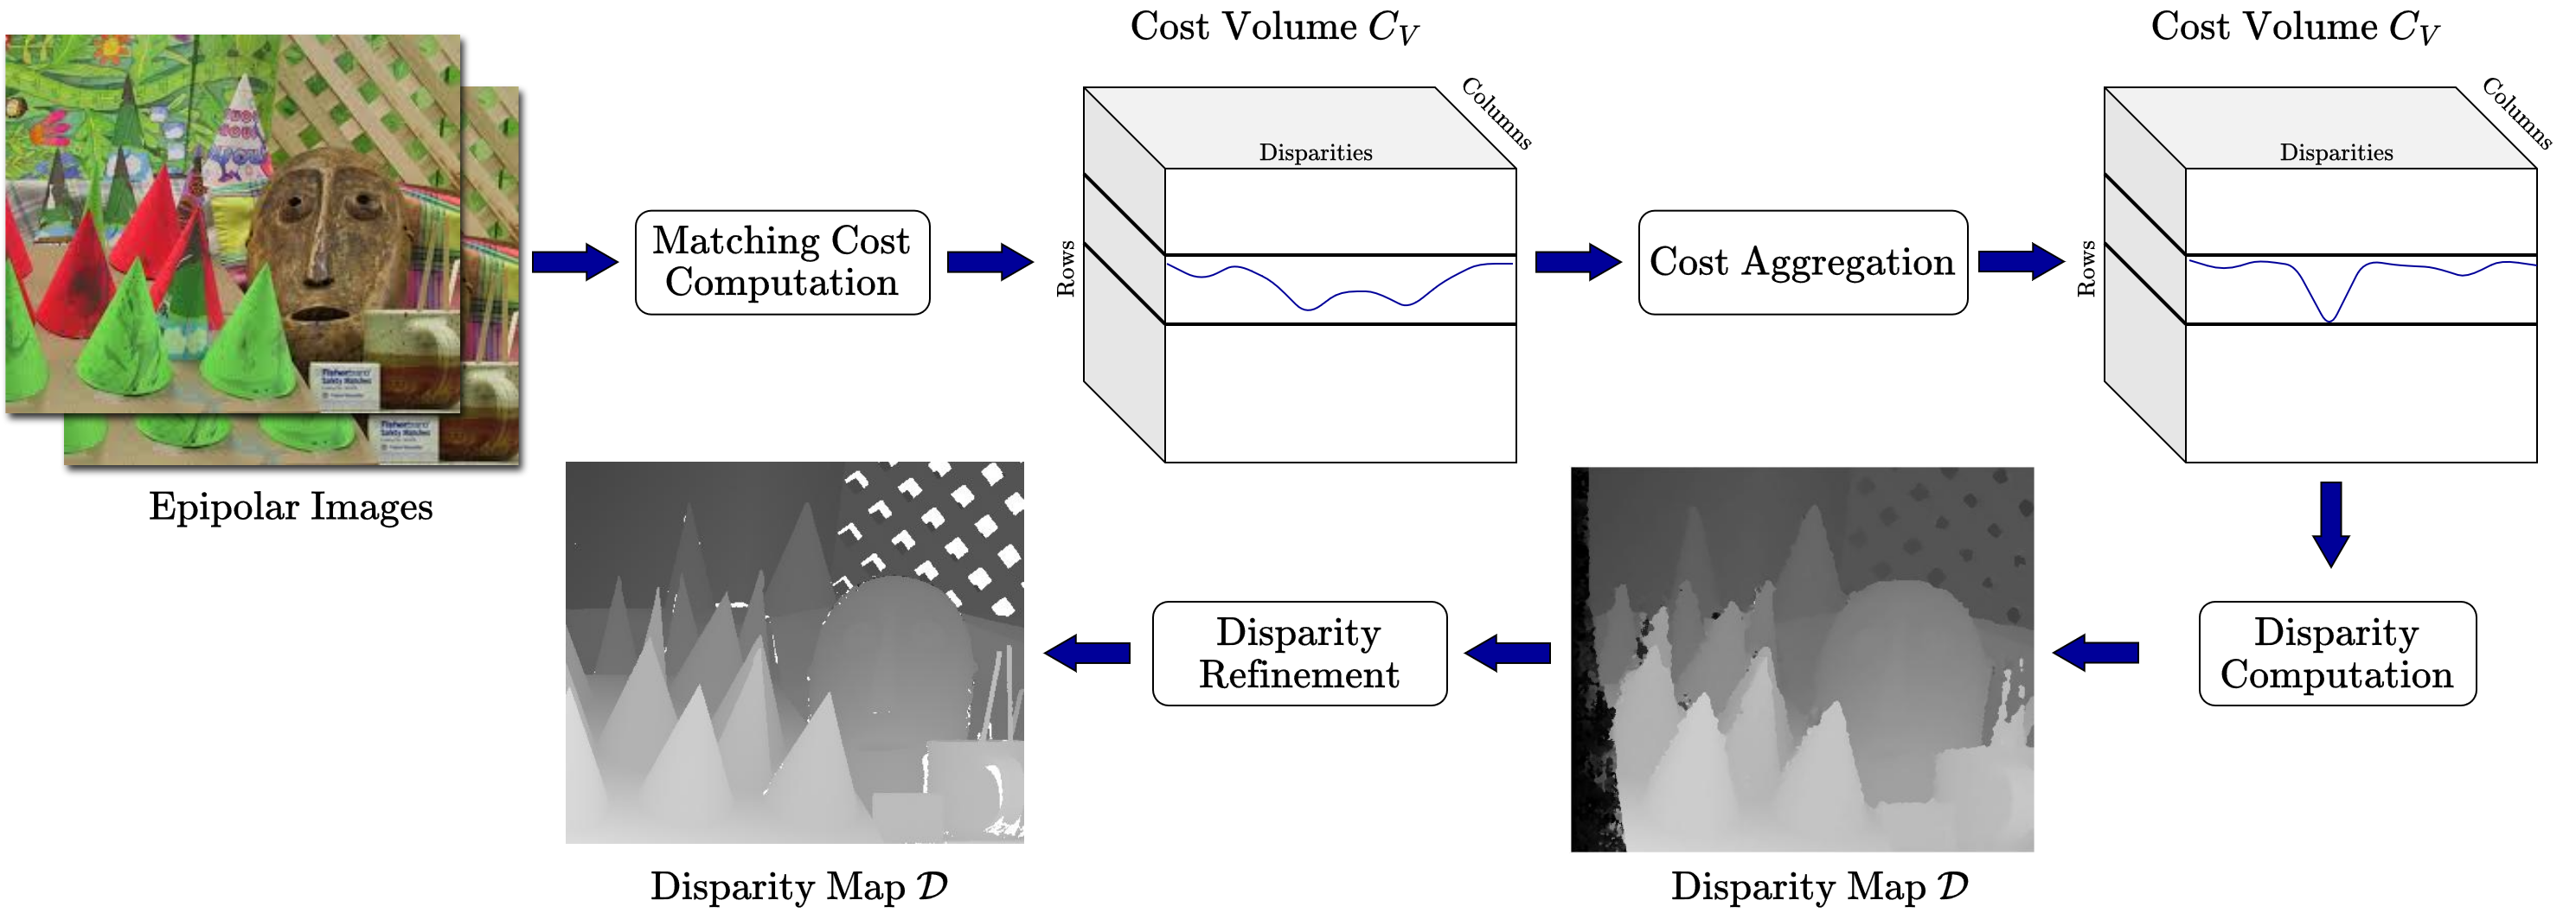
\includegraphics[width=\linewidth]{Images/Chap_1/stereo-matching_pipeline.png}
	\caption{The different steps of classical dense stereo-matching algorithms.}
	\label{fig:stereo_matching_pipeline}
\end{figure}

\subsubsection{Cost Volume Computation}\label{sec:cost_volume_computation}
The cost volume computation can be described as follows: given a range of considered disparity, the cost of matching every pixel of the reference image to every pixel in of the secondary image in the disparity range is stored in an array of data called cost volume (\Cref{fig:cost_volume})\commanue{Avant de dire que c'est stocké dans un cost volume, je dirais que le coût représente la similarité entre deux pixels des deux images. Dans cette première phrase tu mentionnes beaucoup le terme de coût }. The matching cost is evaluated using a cost function, which is a mapping $f$ from subsets of the left and right images to $\mathbb{R}$\commanue{Tu peux peut-être rajouter que la focntion de coût est là pour donner un score sur la similarité entre les pixels de deux images avant de te lancer dans les exemples}. Example\commanue{C'est bizarre le terme example} \ref{ex:cost_functions} provides different examples of cost functions\commanue{Peut-être ajouter une définition générique de la fonction de coût avant de parler des exemples}.

\begin{example}\label{ex:cost_functions}
	Simple examples of cost functions include the Sum of Absolute Differences (SAD), the Zero Normalized Crossed Correlation (ZNCC)  \cite{hannah_computer_1994}, the CENSUS transform \cite{zabih_non-parametric_1994} and MC-CNN \cite{zbontar_stereo_2016}.
	
	Given two windows $W_L$ and $W_R$ from the left and right images, the SAD cost function is defined as follows:
	\begin{equation}
		f_{SAD}(W_L, W_R)  = \sum_i\sum_j | W_L(i,j) - W_R(i,j) |
	\end{equation}
	Low $f_{SAD}$ values indicate that the windows are similar, while high values indicate noticeable differences. A $f_{SAD}$ value of $0$ indicates that the windows are identical. This cost function is probably the simplest cost function one could imagine, and will be used to detail\commanue{le to detail est en trop à mon sens car tu as déjà une autre verbe après} in \Cref{chap:propagating}\comloic{juste used in chapter 4 to didactically} to didactically illustrate how uncertainty models can be propagated throughout a cost function. However, this cost function is not usually used\comloic{usually used? ;-) en gro c'est pas robuste à un bias radio entre les images ni un offset, or meme dans les conditions CO3D (et déjà c'est synchrone ou quasi et pas commun), tu as des objets imagé a la meme heure mais selon l'angl de prise de vue la radio peut différer donc SAD dans les chous}\commanue{in practice ?} in stereo matching algorithms as more efficient cost functions have been proposed since\commanue{tu pourrais juste préciser que ce n'est pas efficace car juste baser sur des différences radio}. It can be a fast and easy way to have a first estimate of similarities between multiple patches. The SAD can also be used for motion estimation and image/video compression \cite{richardson_h264_2006}.
	
	The ZNCC cost function is defined as the correlation coefficient between both images:
	\begin{equation}
		f_{ZNCC}(W_L, W_R)  = \sum_i\sum_j \frac{(W_L(i,j)  - \tilde{W}_L) (W_R(i,j)  - \tilde{W}_R) }{\sigma_L\sigma_R}
	\end{equation}
	where $\tilde{W}$ refers to the mean value of a window, and $\sigma$ its standard deviation. Negatively correlated windows would present a ZNCC value of $-1$ and positively correlated windows present a ZNCC value of $1$. Contrary to the SAD cost function, matching windows will be indicated by a high value of the ZNCC. It is thus not \textit{strictly} a cost function but rather a similarity function. It is not a problem, as multiplying $f_{ZNCC}$ by $-1$ will transform it into a cost function. Another formulation could be to say that the $ZNCC$ is a \textit{maxitive} cost function, in the sense where potential matches are found by searching for its maximum. Conversely, the SAD is a \textit{minitive} cost function in the sense where potential matches are indicated by a minimal cost.\commanue{Avantages? Inconvénients? Est-ce qu'on l'utilise? Non, ça présente pas mal d'intérêt notamment dans les zones homogènes mais pour CO3D on vise des trucs sympas en urbain vu que bon, l'argent il est là... donc il faut pas trop baver enfin adhérer, donc on préfère census}
	
	The CENSUS cost function\comloic{à l'oringe c'est un filtre, Census Filter, ça devient dans le langage commun une cost function juste parce que si tu l'applique à deux images et que tu ajoutes la distance de hamming bein ça marche bien} needs a bit more detailing\commanue{mon anglais pourri penche pour needs to be a little more detailed}\comloic{+1}. For a squared window $W$ with a side of $2n+1$ pixels, we first compare the value of each pixel of the window with the center pixel. This gives a binary string where $1$ indicates that the value of the pixel is superior to that of the center pixel. For instance if we consider the two $3\times3$ following windows $W_L, W_R$:
	$$
    \begin{bmatrix}
        155 & 133 & 97 \\
        80 & 110 & 132 \\
        100 & 102 & 120
    \end{bmatrix}
    \qquad
    \begin{bmatrix}
        175 & 153 & 133 \\
        100 & 130 & 152 \\
        120 & 135 & 125
    \end{bmatrix}
	$$
	Then comparing each of their pixel to the center of the windows will yield the following binary strings (expressed here as matrices):
	$$
    \begin{bmatrix}
        1 & 1 & 0 \\
        0 &  & 1 \\
        0 & 0 & 1
    \end{bmatrix}
    \qquad
    \begin{bmatrix}
        1 & 1 & 1 \\
        0 &  & 1 \\
        0 & 1 & 0
    \end{bmatrix}
	$$
	The cost function $f_{CENSUS}$ is finally obtained by taking the Hamming distance (\ie the number of different bits between those two strings:
	\begin{equation*}
		f_{CENSUS}(W_L, W_R) = 3
	\end{equation*}
	
	The CENSUS cost function compares relative intensity variations, it is thus less sensitive to variations of intensities between images, such as a change of exposure for instance. Similarly to the SAD, two similar patches will tend to have a low value.
	
	The MC-CNN cost function \cite{zbontar_stereo_2016} is using a convolutional neural network architecture to measure the similarity between patches\commanue{ça mérite un peu de schémas}\comloic{la partie convolutionnelle elle permet de décrire un patch, un peu comme un descripteur sift quoi, après il y a une mesure de similarity (cosine similarity) branchée derrière et une loss qui force la sortie du nn à tendre vers des patchs utiles pour le matching en particulier}. It was train on $11\times 11$ patches from stereo images from the Kitti \cite{geiger_vision_2013, menze_object_2015} and Middlebury \cite{scharstein_taxonomy_2001,scharstein_high-accuracy_2003,hirschmuller_evaluation_2007,scharstein_learning_2007,scharstein_high-resolution_2014} datasets. They first trained their network to compute a vector of features for each patch\commanue{Modèle siamois même réseau pour extraire les features entre les iamges}. They then trained a second network to compute the similarity measure between both feature vectors. They also proposed a so-called ``fast'' architecture, which directly computes the cosinus between both vectors, thus by-passing the need of a second network for similarity\commanue{Avec le cosinus simple produit scalaire donc}\comloic{ok tu précises des choses ici, mais du coup plus haut, au moment ou tu dis MCCNN c'est un CNN pour mesurer la similarité c'est pas trop ça... enfin faut choisir, MCCNN c'est soit un outil, celui du papier, soit un réseau de neurones mais qui ne sort pas une mesure de similarité il sort juste un descripteur à la sift}. As ZNCC, MC-CNN is a similarity measure\comloic{ok donc soit c'est une mesure de similarité, mais alors là c'est pas juste un convolutional neural network, c'est soit l'enchainement de deux cnn soit un cnn et une vraie mesure de similarité qui n'a pas besoin de MCCNN pour être une mesure de similarité d'ailleurs}, but can easily be converted into a cost function. Although it has been trained on stereo images of autonomous cars (Kitti) and stereo images of toys (Middlebury), it generalizes well to our satellite images\commanue{cite la publi de Véro et Loïc}.
\end{example}
	
Using the chosen cost function $f$, a cost volume $C_V$ is then evaluated by measuring the cost of matching every patch in the left image to every pixel in the right image in the given disparity range\commanue{ça ressemble bcp à l'intro, donc je pense que ton intro devrait démarrer par la fonction coût et ensuite tu embrailles comme tu le fais avec le cost volume}. The cost volume as thus three dimensions, namely rows, columns and disparity:
\begin{equation}\label{eq:cost_volume}
    C_V(row, ~col, ~d) = f(W_L(row, ~col),  W_R(row, ~col+d))
\end{equation}
where $W_L(row, ~col)$ is a window centered on the pixel at coordinates $(row, ~col)$ in the left image, and $W_R(row, ~col+d)$ is a window centered on the pixel at $(row, ~col+d)$ in the right image. We usually add some padding to the images to avoid problems near borders where the column $col+d$ would not be defined. Given a pixel in the left image $(row, ~col)$, matching cost values for every considered disparity form what is called a cost curvecurve. In theory, the correct disparity for a match is determined by finding the minimum of the cost curve (for minitive cost functions such as SAD or CENSUS). In the rest of this thesis, we will consider that a cost function is always minitive unless specified otherwise. In practice, directly determining correct disparities from the cost volume is not efficient as geometric structure of the scene is not yet taken into account\commanue{Je ne suis pas sure de comprendre. Tu veux parler du fait que sans optimisation on a pas de bons résultats ? C'est pas évident de voir ce que tu sosu-entends par prendre en compte la géométrie de la structure étant donné que c'ets justement ce qu'on cherche a estimé. Peut-être dire juste préciser le meilleur candidat donc approche locale sans tenir compte du voisinage des disparités ne donne pas des choses terribles et donc un exemple pour montrer que c'est très bruité.}. \Cref{fig:cost_volume} represents a cost volume, and one of its cost curves where potential matches have been highlighted\commanue{peut-être mettre cette phrase avant quand tu définis les termes. Ensuite tu pars sur des remarques pour revenir sur un schéma}. 

\begin{figure}
	\centering
	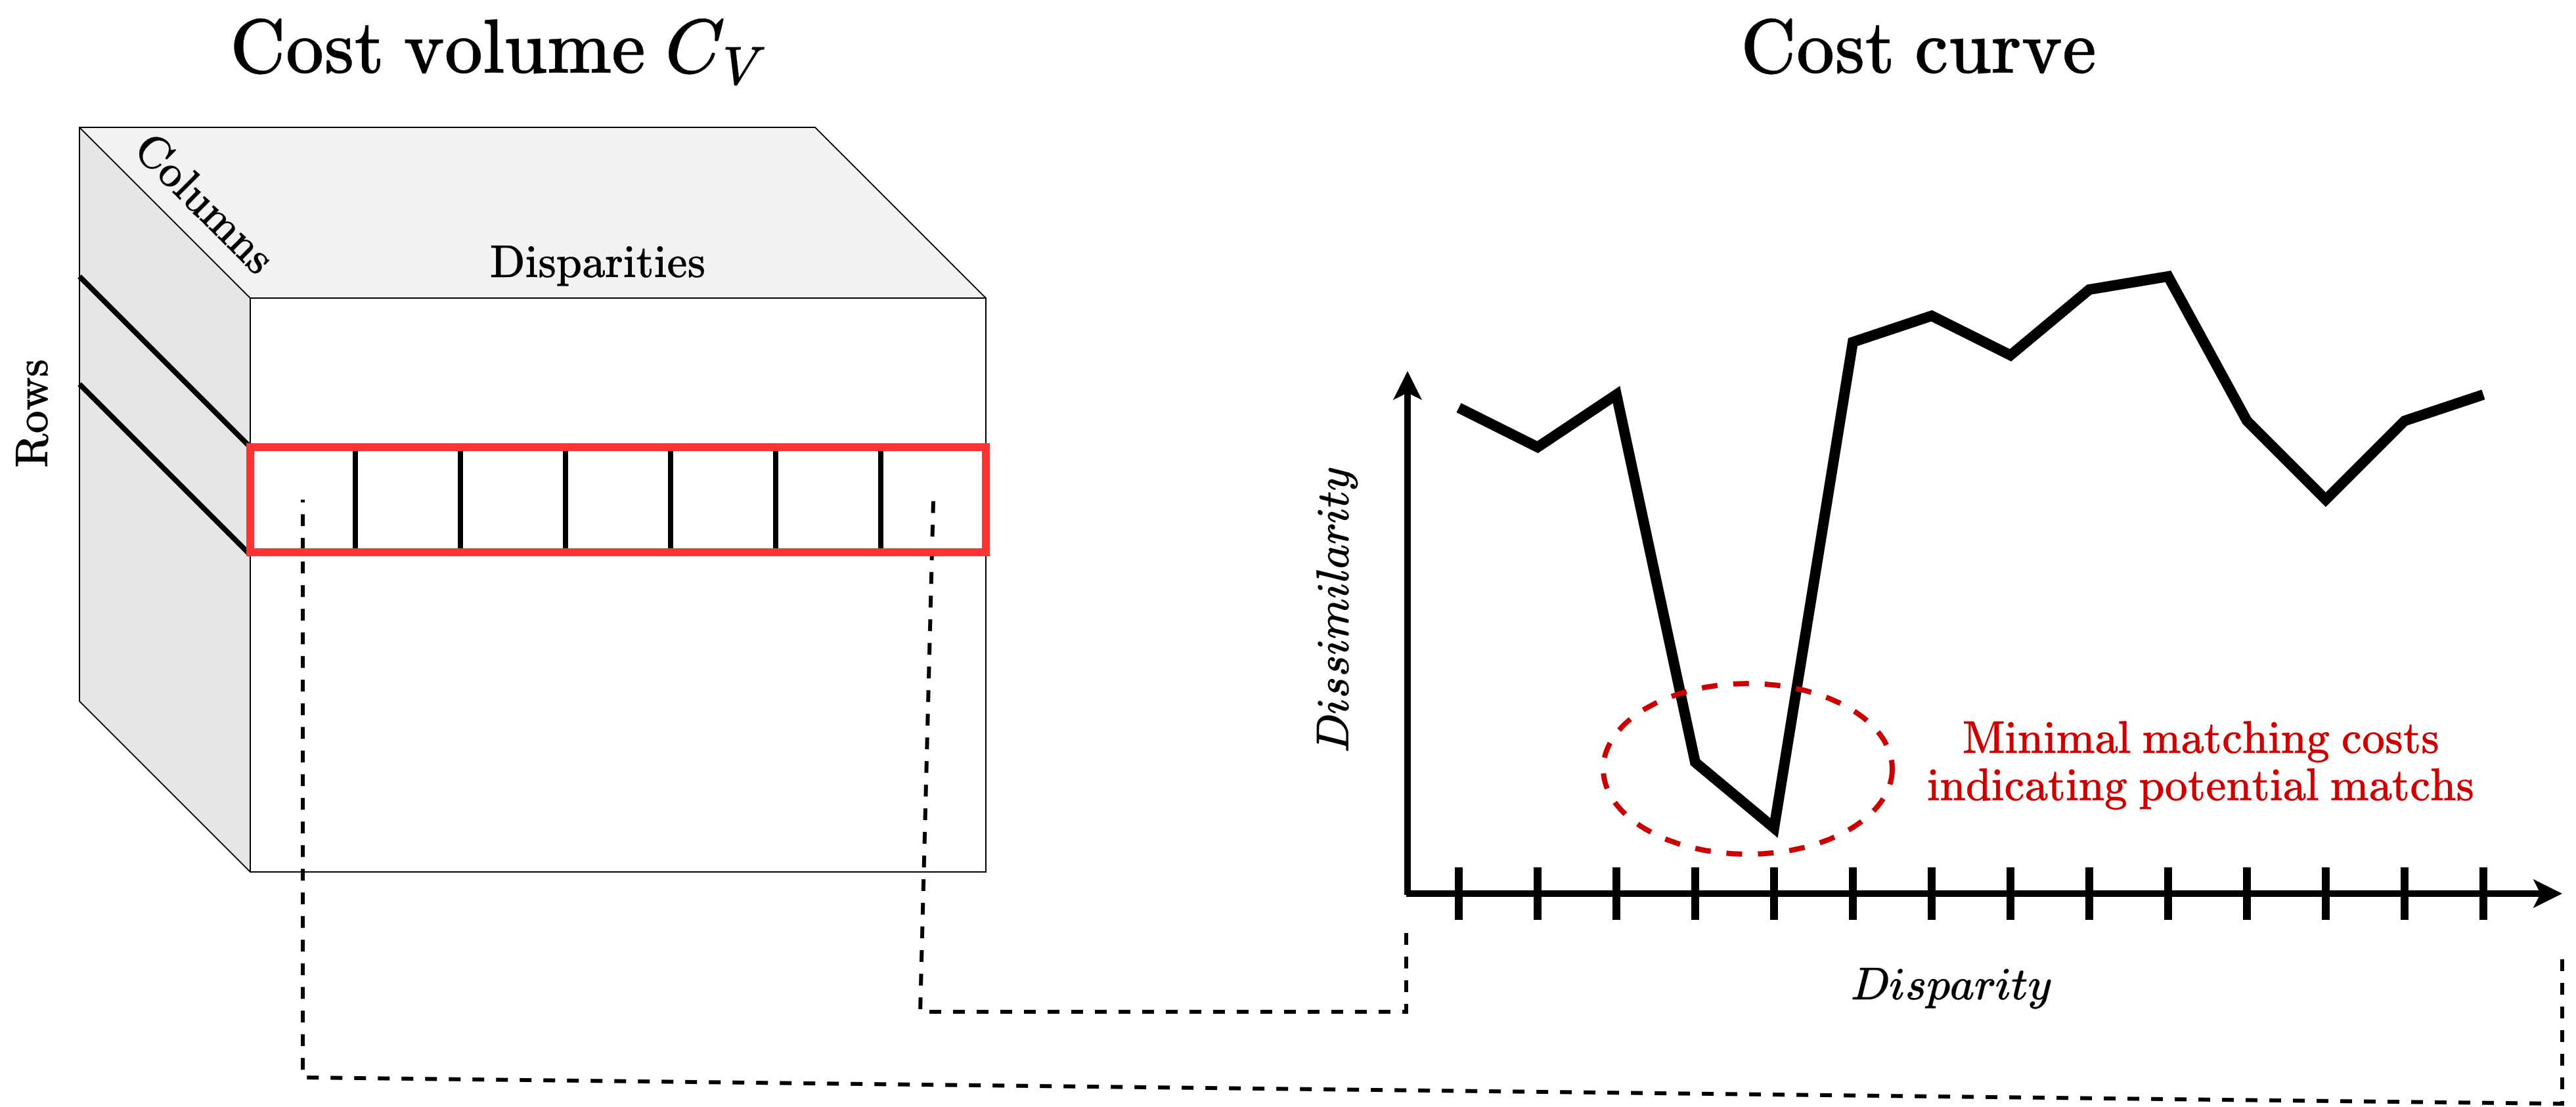
\includegraphics[width=\linewidth]{Images/Chap_1/Cost_volume.png}
	\caption{Matching cost volume and one of its cost curve}
	\label{fig:cost_volume}
\end{figure}\commanu{dans le texte de la figure: minimal matching cost indicating potential match, sans pluriel. ou sinon matchs-> matches}

The usage of windows\commanue{in the calculation of the cost function} allows to take into consideration the surrounding of pixels to better measure their similarity. However, window based approaches\commanue{ajouter peut-être: , mostly square-shaped,} also present the disadvantage of struggling to correctly identify matches near object borders \cite{hirschmuller_real-time_2002}. This is usually called an adherence effect, represented in \Cref{fig:adherence_window}\commanue{Pour montrer l'adhérence il te faut aussi un schéma en 3D pour que les gens comprennent bien ce que voit l'image de gauche et celle de droite. Après tu peux rester 1D pour que ce soit plus simple. Il te faut aussi (oui c'est relou l'adhérence) le résultat en terme de disparité pour montrer pourquoi on appelle cela adhérence}. In this figure, there are three objects represented with three different colors. Centered pixels of both windows do not match, contrary to the rest of the windows which are exactly the same. Sliding the right window in both directions would lead to higher matching costs, as the windows would be even more dissimilar\commanue{je ne suis pas sure de comprendre la phrase. L'adhérence c'est justement que tu vas te retrouver à trouver qu'à cause du voisinage tu vas pas associer le bon pixel. En général tu descends du building un peu plus tard que dans la réalité. En fait ce qu'il te manque dans ta figure c'est qu'est-ce qu'il faudrait associer comme bonne disparité et qu'est-ce que tu as associé en fait du fait de la fenêtre utilisée.}. This illustrates the fact that matching windows do not necessarily mean that the center pixels constitute a match. Other work have been proposing to use a spatial weighting \cite{kuk-jin_yoon_locally_2005}, segmentation \cite{hutchison_segmentation-based_2007}, windows with different shapes \cite{ke_zhang_cross-based_2009, buades_reliable_2015} to solve this problem. 
\begin{figure}
	\centering
	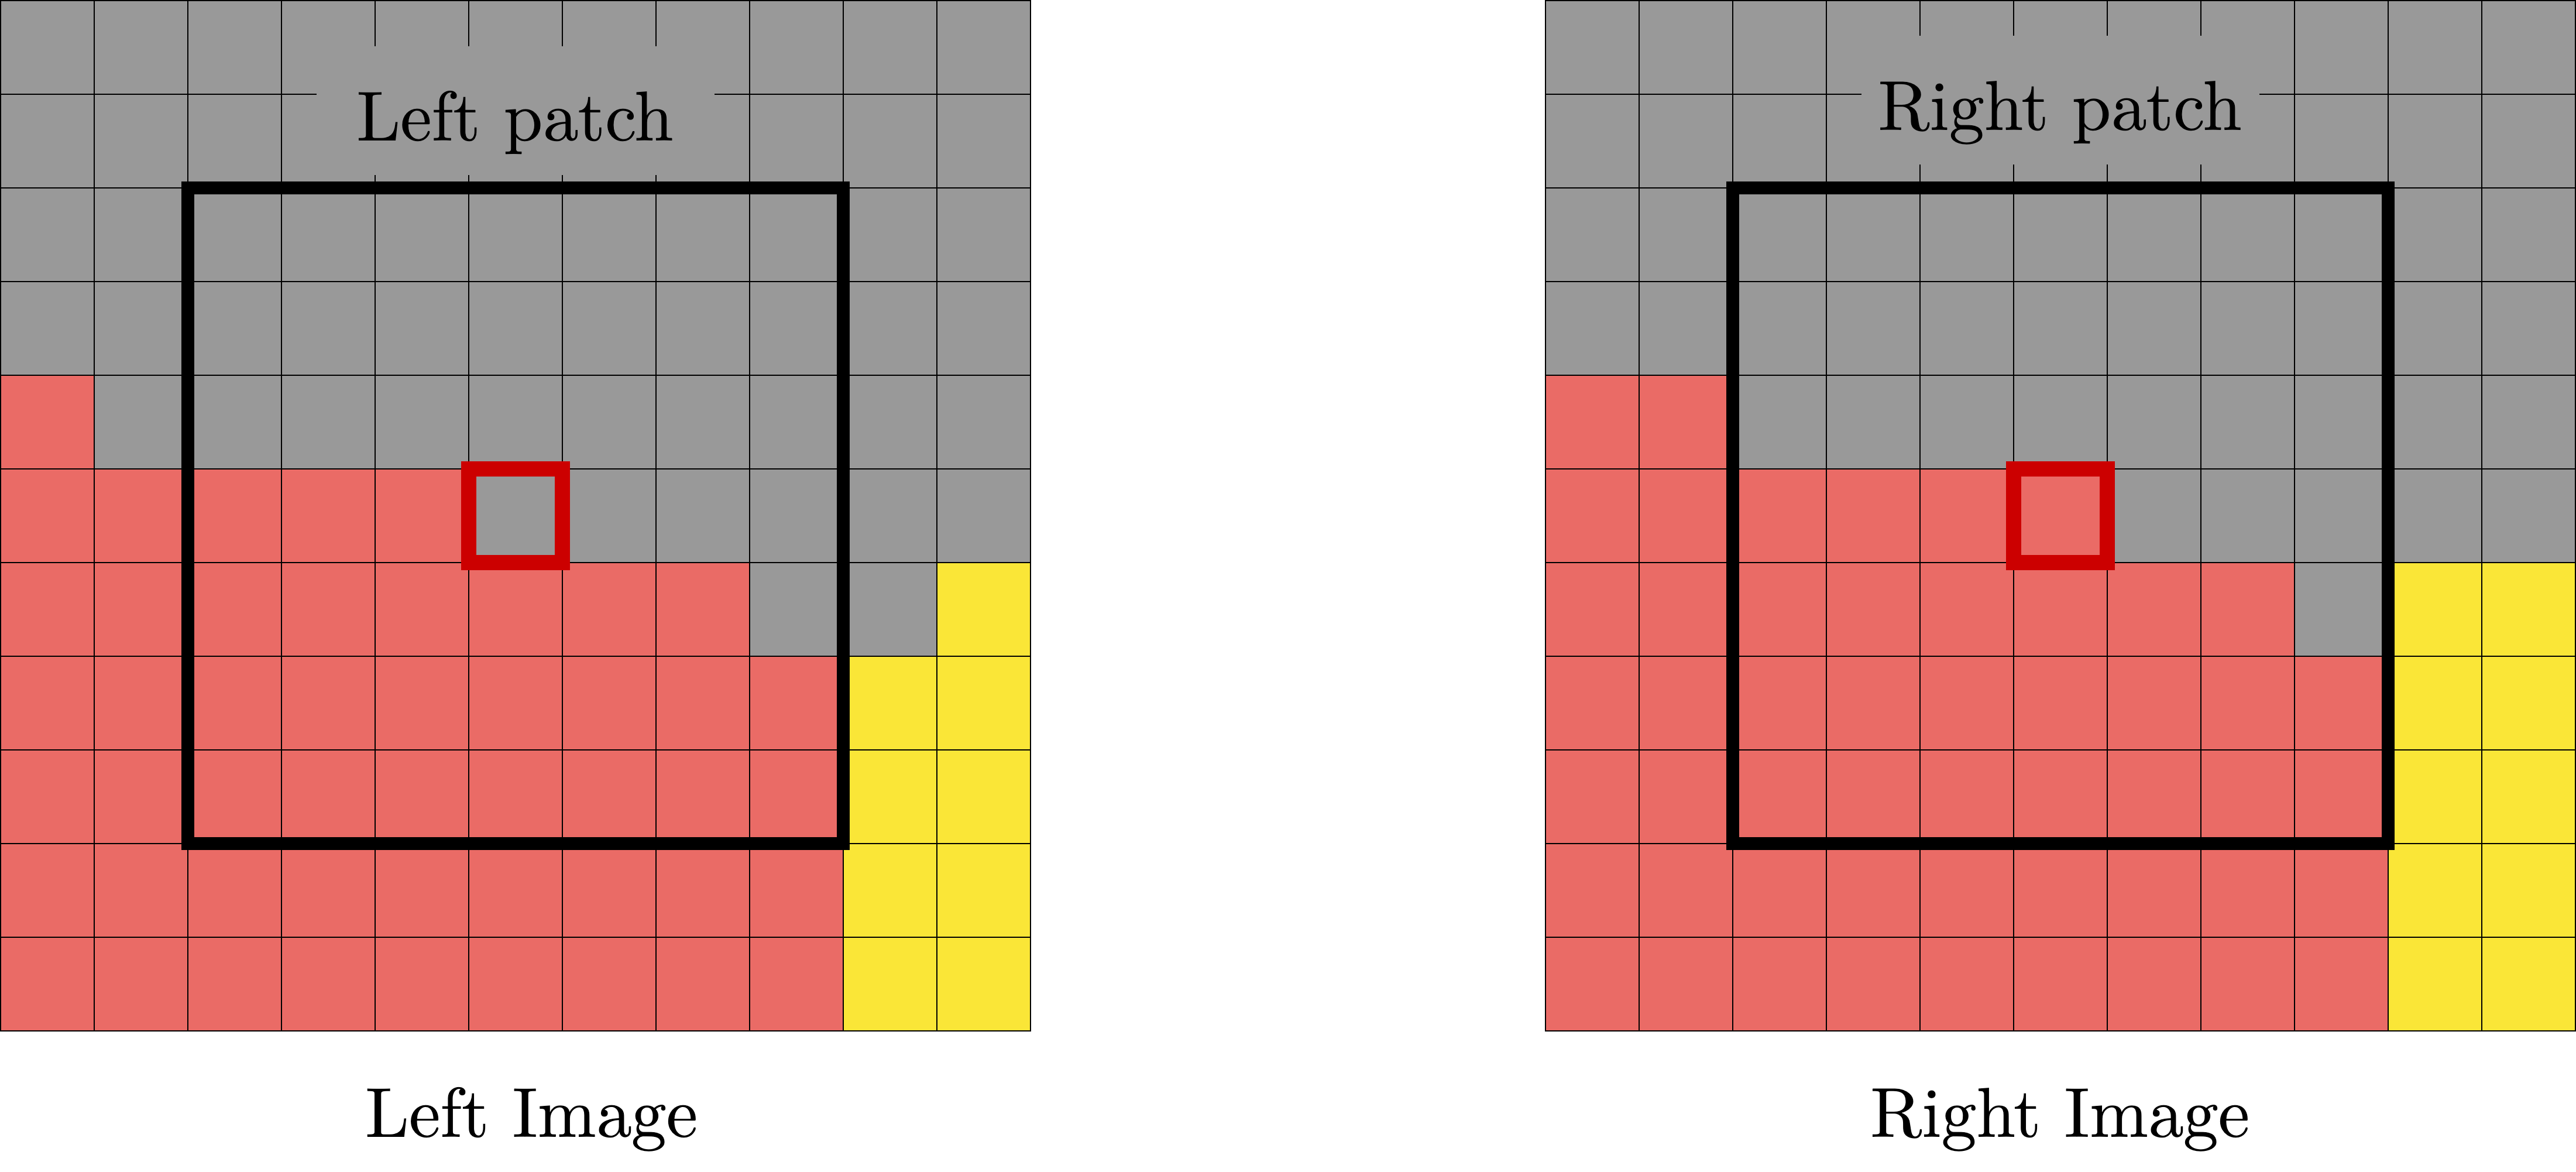
\includegraphics[width=\linewidth]{Images/Chap_1/Adherence_window.png}
	\caption{Adherence problem when comparing two patches between epipolar images}
	\label{fig:adherence_window}
\end{figure}

After computing the matching cost, information regarding the geometric structure of the scene\commanue{c'est pas ton meilleur choix de terme} can be incorporated in the cost volume. A first approach is to aggregate different parts of the cost volume. Usually, costs of pixels belonging to the same objects are aggregated using different methods for segmentation \cite{ke_zhang_cross-based_2009, ji_superpixel_2021}. This part is not always present in algorithms, as we will see next there exists regularization algorithms designed with the same purpose. 

\subsubsection{Semi Global Matching and Disparity Computation}
\commanu{comme dit au début de la partie dense matching, pas évident de retrouver l'ordre de présentation du début. etre cohérent avec le déroulé du début du dense matching, sinon pas évident de suivre pour un lecteur}
Computing the disparity map from the cost volume can be done in several ways. So-called local methods apply a direct \textit{winner-takes-all} strategy, where the $\argmin$ of every cost curve is kept as the selected disparity. This has the disadvantage on allowing multiple pixels from the right image to be matched to the same pixel of the left image\comloic{je vois pas trop pourquoi ça ne peut être le cas pour une méthode globale ? je rate un truc ?}. On the other hand, global method use the information contained in the cost volume to solve an optimization problem, where the objective is to compute the disparity map $\mathcal{D}$ minimizing an energy function expressed as follows:
\begin{equation}
    E(\mathcal{D}) = E_{data}(\mathcal{D}) + \lambda E_{smooth}(\mathcal{D})
\end{equation}
where $\lambda$ is a scalar for tuning the importance of the regularization term $E_{smooth}$. Usually, the data term is directly computed from the cost volume as:
\begin{equation}\label{eq:global_methods}
    E_{data}(D) = \sum_{row,~col}C_V(row, ~col,~D(row, ~col))\commanue{C'est pas le même symbole D que dans la précédente équation}
\end{equation}
The regularization term $E_{smooth}$ can take numerous forms, usually measuring if the neighbouring disparities possess similar values \cite{scharstein_taxonomy_2001}. Then a local minimum for this energy is found using various methods, such as Markov Random Fields \cite{boykov_markov_1998, sun_stereo_2003}, graph cuts \cite{kolmogorov_computing_2001} or minimum spanning trees \cite{zureiki_stereo_2008, qingxiong_yang_non-local_2012}. Those algorithms improves performances in comparison to local methods, but can be computationally expensive.

The most popular method is actually Semi-Global Matching (SGM) \cite{hirschmuller_accurate_2005}: it aims at incorporating regularization constraints to the cost volume similarly to global methods, in order to be processed\commanue{j'aurais tendance à mettre while being processed with relative low computational cost pour montrer que SGM cherche à avoir les avantages des deux côtés}\comloic{ouais parce que il y a aussi un cost volume dans de vraies méthode globale genre basées sur les graphes et résolue par komlogorov ou son copain donc là c'est surtout que c'est semi global parce qu'on résoud pas le problème initial on fait une modélisation simplifiée en réduisant tout ça a quelques chemins} like local methods. It is, in a way, in-between local and global methods. This is the method we will\commanu{j'aurais enlevé le will} use in the CARS pipeline for experiments in this thesis. In short, for each pixel, the SGM algorithm looks into neighbouring pixels recursively, and increases the cost of disparities that do not present a consensus\comloic{pas sur de te comprendre?} amongst neighbours \comloic{je pense que si tu veux être rigoureux tu dois présenter le CV comme un graphe, avec les noeuds qui sont le terme Edata c'est à dire les couts de similarité et les liens qui sont le termes Esmooth. Ensuite SGM dit simplement "je vais pas résoudre le problème dans sa globalité je vais le réduire à une dimension et répéter 4/8 fois ce job pour 4/8 directions}. Although the formulation of the SGM algorithm can be expressed in a few equations, understanding how its inner workings is more complex. We will first present its mathematical formulation in \cref{eq:sgm,eq:sgm_penalties}, and use \Cref{fig:sgm} to illustrate its effect on (a portion of) a cost curve. Formally, for every pixel $p=(row, ~col)$, the cost volume is explored in multiple directions as in \Cref{fig:sgm_directions}.

\begin{figure}
	\centering
	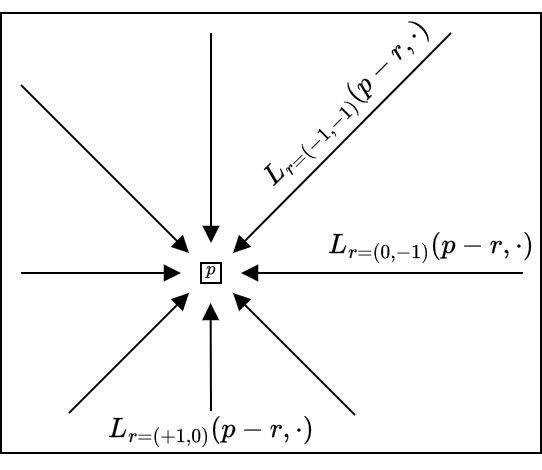
\includegraphics[width=0.5\linewidth]{Images/Chap_1/SGM_directions.png}
	\caption{SGM regularization with $8$ directions}
	\label{fig:sgm_directions}
\end{figure}

The cost is regularized for each direction $r$ to take into account the best disparity $d$ along that direction. A direction can be for instance $r=(0,~1)$, meaning that we will look at same row and travel to the right of the image when browsing direction $r$. Given two positive scalars $P_1<P_2$, the regularized cost $L_r$ along direction $r$ and at disparity $d$ is expressed with the following recursive formulation:
\begin{align}\label{eq:sgm}
    L_r(p,d) = C_V(p,d) + \min_\delta \left(L_r(p-r,~\delta) + R(d, ~\delta)\right)\commanue{elle est bizarre la formulation de SGM. Je comprends le $\delta$, c'est pas évident de retrouver la formule de l'article}
\end{align}
where $R(d, ~\delta)$ equals:
\begin{align}
    R(d, ~\delta) = &P_1\cdot\mathds{1}(|d-\delta|=1) + P_2\cdot\mathds{1}(|d-\delta|\geqslant 2) - \min_k L_r(p-r,~k) \label{eq:sgm_penalties}
\end{align}
Here, $\mathds{1}$ is the indicator function. The first term of \cref{eq:sgm} is the cost volume, which can be compared to $E_{data}$ in \cref{eq:global_methods}. The second term is similar to the regularisation term $E_{smooth}$. This term can be seen as the regularized cost $L_r(p-r, ~d)$ from the previous pixel in direction $r$, but shifted of $P_1$ for neighbouring disparities $d\pm1$, and of $P_2$ for further disparities. The term $\min_k(L_r(p-r,~k))$ prevents $L_r(p,\cdot)$ to diverge to very high values by ensuring that the minimum of $L_r(p-r,~\delta) - \min_k(L_r(p-r,~k))$ always equals $0$. \Cref{fig:sgm}\commanue{J'avoue que j'ai du relire le paragraphe plusieurs fois, j'ai un peu  de mal avec ta notation qui se veut très générique. C'est un peu le même prinicipe pour la figure. C'est ton choix donc à voir si ça parle plus aux autres.}\commanu{en effet pas évident. peut etre un exemple plus concret sur ce que ca permet de faire et donc de mieux comprendre la motiv de l'algo et donc l'algo in fine. mais pas évident de toute façon de bien l'expliquer} presents $L_r(p-r,~\delta) + R(d, ~\delta)$ for two different disparities $d$ and $d+1$ in the blue frame. The minimum of each curve $L_r(p-r,~\delta) + R(d, ~\delta)$ (blue arrows in the figure) are then added to the matching cost $C_V(p,d)$ to obtain the final regularized cost $L_r(p,d)$. Note that in \Cref{fig:sgm}, the minimum of $L_r(p-r,~\delta)+R(d+1, ~\delta)$ equals $0$, thus $C_V$ is unchanged for this disparity. This is because $d+1$ is the minimum of $L_r(p-r,~\cdot)$. In a way, the regularized matching cost will be a mixture between $C_V(p,\cdot)$ and $L_r(p-r,~\cdot)$. Indeed, the regularized cost $L_r(p-r,\cdot)$ indicates that disparity $d+1$ seems likely, while disparity $d$ is unlikely. On the other hand, the matching cost $C_V(p,\cdot)$ indicates that both disparities $d$ and $d+1$ are likely. The final regularized cost $L_r(p-r,\cdot)$ takes into account that both $C_V(p,\cdot)$ and $L_r(p-r,\cdot)$ agree that $d+1$ is likely, but that there is a disagreement on $d$, and thus slightly increases the regularized cost $L_r(p,d)$. Disparities that seem unlikely to both $C_V(p,\cdot)$ and $L_r(p-r,\cdot)$ lead to a larger increase of the regularized cost $L_r(p,\cdot)$ \commanu{mieux sur la fin, ca pourrait donc etre illustré avec un cas plus concret. Ta figure de l'enfer explique l'algo mais on a a du mal à "voir" ce que ca fait, comme tu l'expliques plutot bien sur cette fin de paragraphe. Donc comme dit, un petit exemple plus concret aiderait}.
\begin{remark}
    For the sake of the remark, let suppose that $P_1=P_2$ for now. The value added to $C_V(p, ~d)$ in \eqref{eq:sgm} will be lower than $P_2$ only if $(L_r(p-r,~d) - \min_k L_r(p-r,~k)$ is less than $P_2$. This means that we will always add a penalty of $P_2$ to the cost $C_V$, except if $L_r(p-r,~d)$ is less than $P_2$ away from its minimum. $P_2$ thus represents the penalty that must be overcame in $L_r(p-r,~d)$ in order to not penalize $C_V(p,d)$, or slightly penalize $C_V(p,d)$.
    
    If $P_1<P_2$, then we can draw similar conclusions, except that we also accept to reduce the penalty to $C_V(p,d)$ if a neighboring disparity, \ie $d\pm1$ is less than $P_1$ away from the minimum. Hopefully this remark, equations and figures helped in making sense of the SGM algorithm\commanu{bizarre ta dernière phrase, pas très anglais, j'enleverais. Par contre, intéressant de donner des cas d'exemples P1=P2, P1 très petit par rapport à P2, et tu pourrais illustrer l'impact sur une petite image bien choisie... suivant le temps bien sur, tu vois}
\end{remark}

Formulation of \cref{eq:sgm} is recursive, and thus must be initialized. The regularization curves thus begin at the borders of the image and their value is, by convention, $0$ when undefined. For instance with $r=(0,1)$:
\begin{align*}
    L_r((row, 0),d) = C_V(row, 0 ,d)
\end{align*} 

\begin{figure}
	\centering
	\includegraphics[width=\linewidth]{Images/Chap_1/SGM.png}
	\caption{Schematic explanation of the SGM algorithm in a single direction $r$. Top: regularized cost $L_r$ at $p-r$. In the blue frame $L_r(p-r,~\delta)+R(d,~\delta)$ for two consecutive disparities $d$ and $d+1$ ($L_r-\min_k L_r$ appears in dotted line for clarity). Penalty $P_1$ appears in yellow, penalty $P_2$ appears in red, the minimum of each curve is denoted by a blue arrow. Bottom left: cost volume $C_V$ at $p$. Bottom right: regularized cost $L_r$ at $p$ where the minima of all $L_r(p-r,~\delta)+R(d,~\delta)$ have been added.}
	\label{fig:sgm}
\end{figure}\comroman{C'est un peu le schéma de l'enfer, mais c'est ce que j'ai trouvé de mieux pour expliquer SGM.}\commanue{comme je le dis plus haut, j'avais que le côté très générique des notations n'ai pas facile. Après il y a des trucs intéressants et de tout façon c'est pas simple à schématiser.}\comloic{est ce que si tu le fais que pour une disparité c'est pas plus simple à présenter ? dans le dernier morceau en rose en bas à droite, j'ai eu du mal à comprendre l'extrapolation de la courbe pour les disparités du point r-1 dont tu ne présentes pas les courbes, ça m'a un peu perturbé. Ou alors tu ne mets à jour que les coeffs des deux disparités étudiées peut être ? Après ce que tu montres c'est la conséquence de l'implémentation mais je sais pas si on capte la motivation. Peut être qu'avec des objets genre bati et sol ou quoi ce serait plus palpable mais enfin c'est pas simple je le reconnais}

When all regularized cost curves $L_r$ have been computed, they are summed to obtained the regularized cost volume $C_V^{SGM}$:
\begin{equation}
    C_V^{SGM}(p, d) = \sum_r L_r(p,d)
\end{equation}
The cost volume $C^{SGM}_V$ contains the regularized cost for\commanue{alors il manque la fin de la phrase} 
Since the original paper \cite{hirschmuller_accurate_2005}, different variations of the SGM algorithm have been proposed. For instance using different regularization paths \cite{facciolo_mgm_2015} or a different strategy for the aggregation of costs \cite{poggi_learning_2016}.

The main problem of SGM regularization is its reluctancy to detect discontinuities in the disparity map. Indeed, SGM penalizes disparity changes, therefore strong variations of disparity are badly reconstructed\comloic{je dirais que ça dépend qd meme fortement de ton termes Esmooth... si P2 et P1 sont tout piti piti piti bah pas de pb sur les bati mais par contre ça reste bien bruité dans les zones homogènes}. For instance near the border of a building, instead of a having the desired discontinuity in the disparity map, there can be a smooth transition \comloic{c'est dommage de pas parler du termes Esmooth ici, tu y es presque avec "smooth". C'est typiquement que SGM n'applique pas le saut de discontinuité tant que Esmooth reste prépondérant devant Edata, le fait que la transition soit progressive c'est plutôt lié à la somme des 8 directions puisqu'elles sont sommées avec le même poids indépendant de la pertinence de ce choix (chemin visible continue entre r-1 et r)} between the roof and the road, leading to rounded borders and soft edges of buildings. This is even reinforced with the window adherence problem presented in \ref{fig:adherence_window}. \Cref{fig:DSM_toulouse} presents a comparison of two DSM: one obtained directly from LiDAR HD data \cite{monnet_lidarhd_2023}, and the other using the CARS pipeline with the CENSUS cost function over a $5\times5$ window and with SGM regularization. We can see on this figure that the border of the buildings obtained using SGM regularization are not as sharp and precise as those of the LiDAR DSM \comloic{alors.. bon... après t'as qd meme une histoire de résolution aussi}. To provide a solution to this problem, one might limit the SGM regularization to pixels from the same object, defined\commanu{bizarre le defined using, je ferais plus direct from the same object using a segmentation} using a segmentation \cite{dumas_improving_2022}. This method relies on the quality of the segmentation method used and can become quite costly. It has not been considered in the context of this thesis. \todoroman{est-ce que c'est prévu de l'utiliser dans le pipeline CO3D? Sinon je peux aussi dire que je ne considère que ce pipeline là}\commanu{à priori oui via 3SGM qui contraint SGM et les segmentation de yannick dans SLURP, c'est en test cette année}

\begin{figure}
    \centering
    \begin{subfigure}[t]{0.5\linewidth}
        \centering
        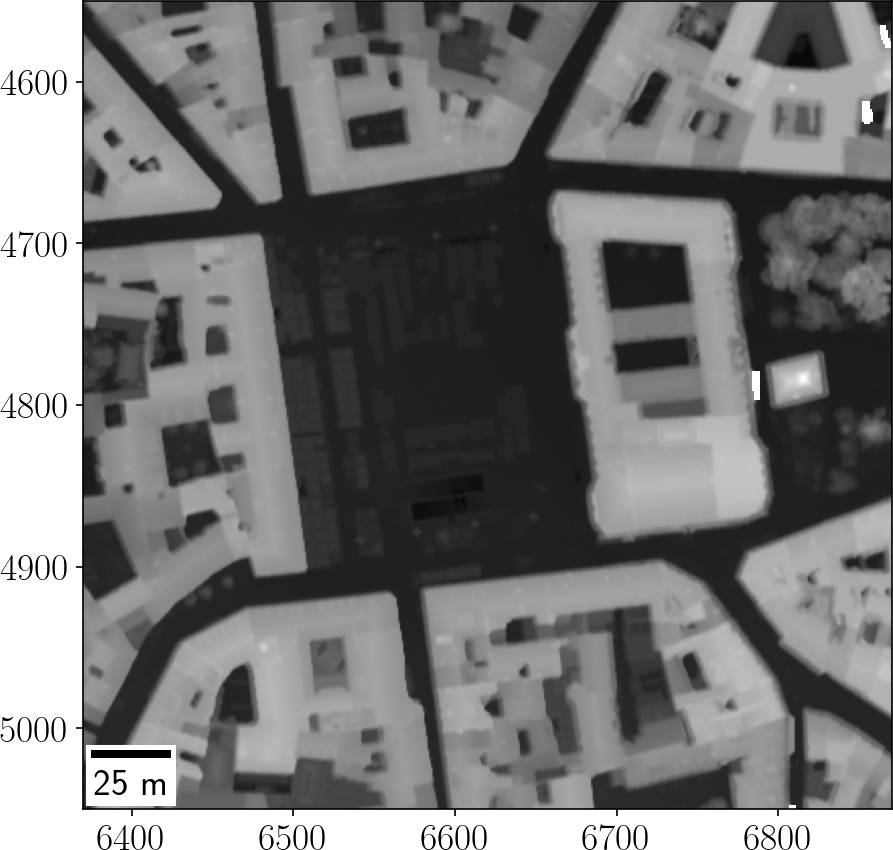
\includegraphics[height=6cm]{Images/Chap_1/DSM_Capitole_LiDAR.png}
        \caption{DSM from LiDAR HD data,\\Place du Capitole}
        \label{fig:DSM_capitole_lidar}
        %\begin{minipage}{.12cm}  % Multiline captions misalign figures
        %    \vfill              % This blank minipage is used to align
        %\end{minipage}          % images
    \end{subfigure}\hfill
    \begin{subfigure}[t]{0.5\linewidth}
        \centering
        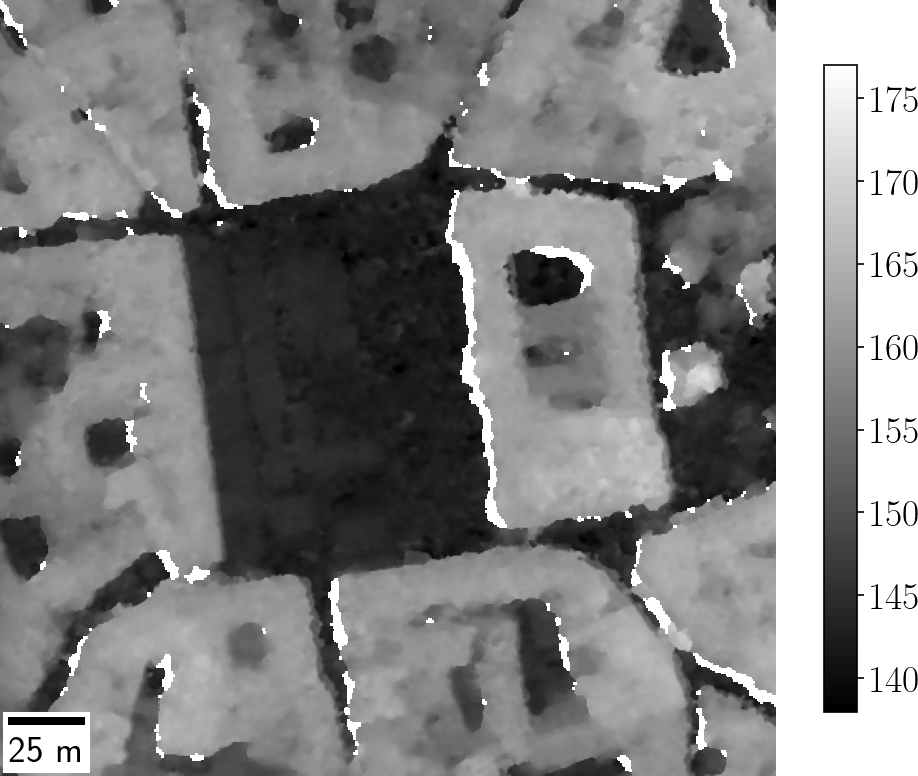
\includegraphics[height=6cm]{Images/Chap_1/DSM_Capitole_CARS.png}
        \caption{CARS DSM from Pléiades images,\\Place du Capitole}
        \label{fig:DSM_capitole_cars}
    \end{subfigure}
    \begin{subfigure}[t]{0.5\linewidth}
        \centering
        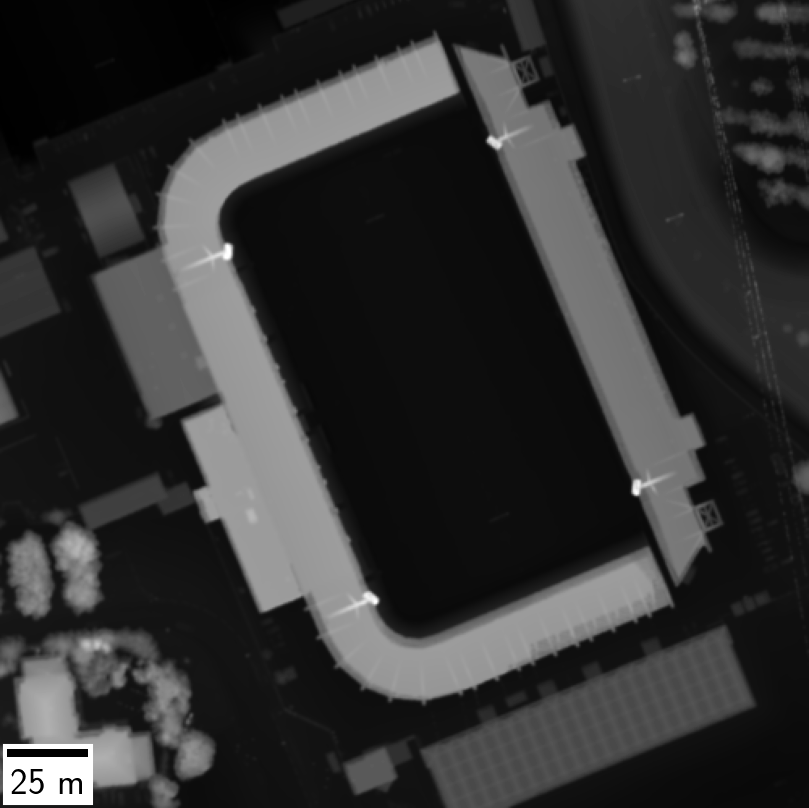
\includegraphics[height=6cm]{Images/Chap_1/DSM_Wallon_LiDAR.png}
        \caption{DSM from LiDAR HD data,\\Ernest Wallon stadium}
        \label{fig:DSM_ernest_wallon_lidar}
    \end{subfigure}\hfill
    \begin{subfigure}[t]{0.5\linewidth}
        \centering
        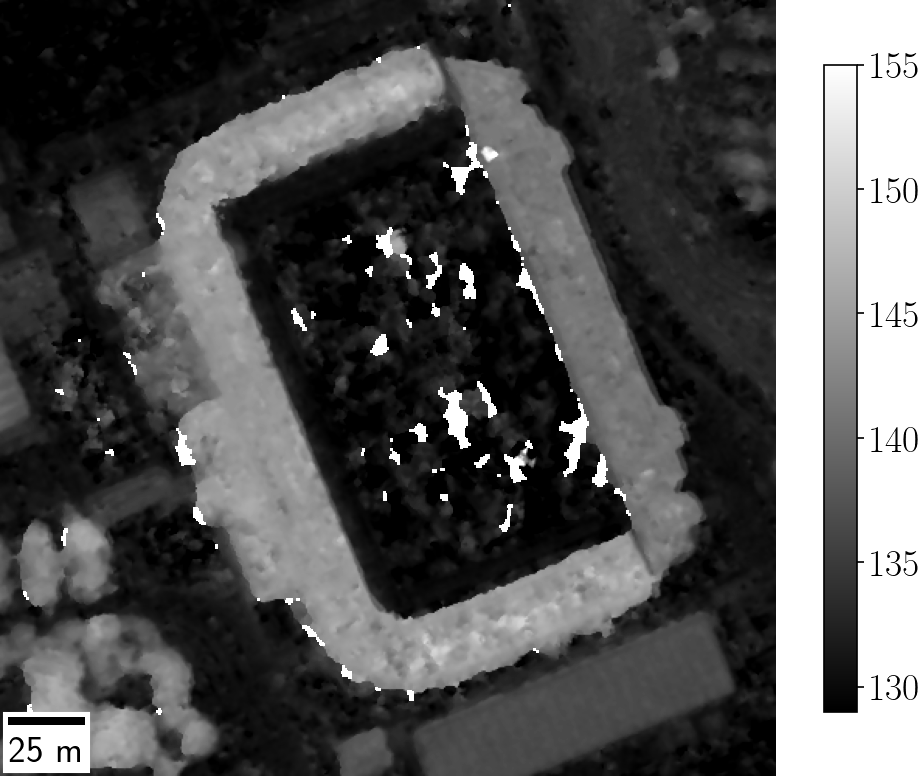
\includegraphics[height=6cm]{Images/Chap_1/DSM_Wallon_CARS.png}
        \caption{CARS DSM from Pléiades images,\\Ernest Wallon stadium}
        \label{fig:DSM_ernest_wallon_cars}
    \end{subfigure}
    \caption{Different DSM over Toulouse, France. DSM were obtained by rasterizing LiDAR HD data or by processing Pléiade stereo images with the CARS pipeline. The CARS pipeline uses a $5\times5$ CENSUS cost function and SGM regularization for stereo reconstruction. \copyright CNES 2017, Distribution AIRBUS DS}
    \label{fig:DSM_toulouse}
\end{figure}


Once the regularized cost volume $C_V^{SGM}$ has been computed, a simple \textit{winner-takes-all} strategy can be used to determine the disparity map $\mathcal{D}$:
\begin{align}
    \mathcal{D}(row, ~col) = \argmin_d C_V^{SGM}(row, col, d) 
\end{align}
\commanu{un peu court sur la stratégie de décision. rien à dire de plus sur l'état de l'art là dessus vu les échanges, et de perpectives? Peut etre juste une phrase du type: Winner takes all is the classical approach taken in literature but other approaches could be interesting to take especially with uncertainty information from this thesis.}

\subsubsection{Processing the Disparity Map}\label{sec:postprocess_disparity}
Once the disparity map has been computed, it is usually post-processed to remove artifacts, and improve disparity resolution.

It is common to add a sub-pixel refinement step, where a non-integer disparity is interpolated around the selected disparity. The main idea is to interpolate a model through the selected disparity $d=\argmin_\delta C_V(row, ~col, ~\delta)$ and its two direct neighbours\commanue{alors j'avais pas remarqué mais tu écris neighbors en anglais UK mais en général tu mets initialize donc c'est anglais US. Donc choisis ton côté de l'atlantique ;)}. The refined disparity $d_{interp}$ is then defined as the $\argmin$ of this interpolation model. \Cref{fig:sub-pixel_refinement} presents examples of interpolated disparities from  \cite{haller_real-time_2010}, mainly a ``V''-like shape as in \ref{fig:vfit_refinement} and a parabola as in \ref{fig:parabola_refinement}. Carrying out sub-pixel refinement suggests we assume the algorithm can attain a significant level of precision, which is debatable (see \Cref{sec:uncertainty_cars})\commanue{Et aussi que la fonction de coût a été suffisamment échantillonnée pour te permettre d'interpoler cotrrectement, ce qu'honnêtement on n'a jamais vérifié. On considère que c'est vrai}.

\begin{figure}
    \centering
    \begin{subfigure}[t]{0.5\linewidth}
        \centering
        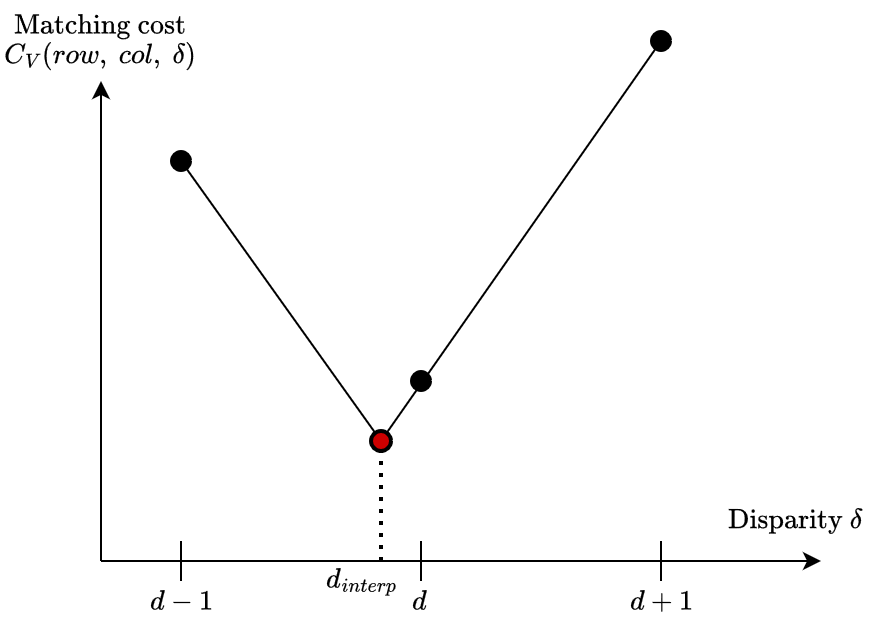
\includegraphics[width=\linewidth]{Images/Chap_1/subpixel_refinment_vfit.png}
        \caption{V-fit sub-pixel refinement}
        \label{fig:vfit_refinement}
    \end{subfigure}\hfill
    \begin{subfigure}[t]{0.5\linewidth}
        \centering
        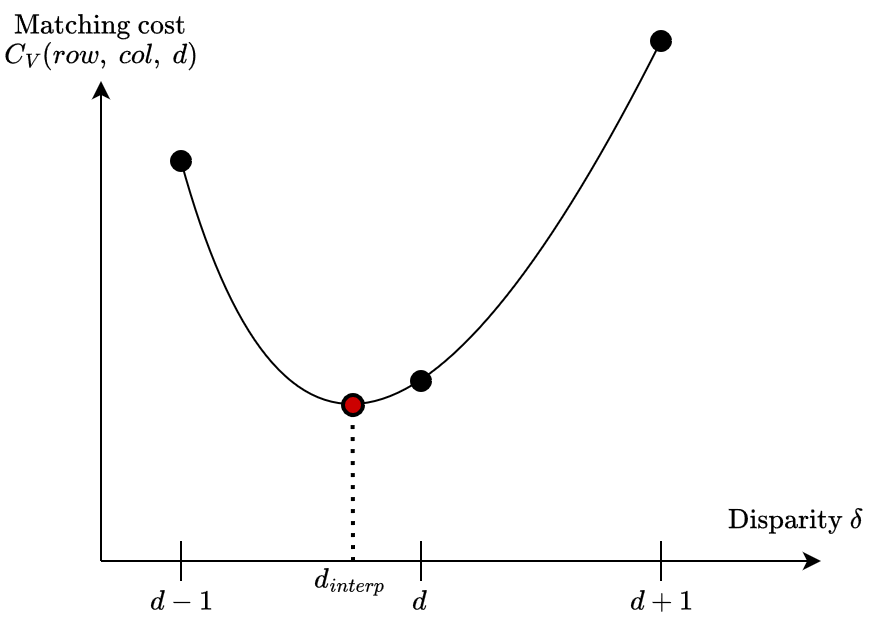
\includegraphics[width=\linewidth]{Images/Chap_1/subpixel_refinment_parabola.png}
        \caption{Parabola sub-pixel refinement}
        \label{fig:parabola_refinement}
    \end{subfigure}
    \caption{Different methods for refining the disparity $d=\argmin_\delta C_V(row, ~col, ~\delta)$}
    \label{fig:sub-pixel_refinement}
\end{figure}

The disparity map can also be filtered in order to remove local outliers. Classical strategies include the use of a mean or median filter for instance. There exists more advance filtering methods, such as bilateral filtering \cite{tomasi_bilateral_1998} which performs a weighted average, where weights depend on the proximity to other pixels both in the spatial and spectral domain.  

As presented previously, the \textit{winner-takes-all} strategy presents the inconvenient of allowing multiple pixels from the secondary image to be matched to the same pixel of the right image. For instance, if two pixels $(row,~col)$ and $(row,~col+1)$ from the second image have $d$ and $d-1$ as their respective disparity, they will be both matched to pixel $(row, ~col+d)$ in the reference image. This effect indicates that there is probably an error in the estimation of the disparity map. There exist strategies allowing to detect such error in order to eliminate dubious matches. A first strategy is called cross-checking \cite{fua_combining_1991}. We first start by computing a secondary cost volume $C_V'$ by reversing the roles of the images: the reference image becomes the secondary image and vice-versa. We then obtain two disparity maps $\mathcal{D}$ and $\mathcal{D}'$, and check that they are consistent, as in theory we would that $\mathcal{D}=-\mathcal{D}'$. A pixel $(row, ~col)$ is considered consistent across disparity maps if it verifies:
\begin{equation}\label{eq:cross-checking}
    |\mathcal{D}(row, col) + \mathcal{D}'(row, col+\mathcal{D}(row, col))|\leqslant \tau
\end{equation}
where $\tau$ is a consistency threshold usually set to $1$. For errors that do not check this consistency check, it has been proposed in \cite{hirschmuller_stereo_2008} to differentiate between mismatched pixels (pixels for which there exists a correct match) and occluded pixels (pixels that visible in an image but masked by an object in the other) as follows: if there is a disparity $d\in\mathcal{D}$ such that $\mathcal{D}'(row, col+d)=-d$ then it is a mismatch\commanue{la phrase est assez longue et en plus tu as des éléments en parenthèses. Il faudrait peut-être mieux splitter les éléments}. Otherwise, pixel $(row, ~col)$ is occluded. Occluded regions of an image can be filled by interpolation with the closest valid disparities\commanue{alors j'ai un doute on rebouche par interpolation avec les voisins les mismatch aussi, non?}.  

\begin{remark}
     \Cref{eq:cross-checking} requires the computation of a second cost volume, effectively doubles the processing time. As dense stereo matching is also the longest part of a photogrammetry pipeline, one might be reticent to carry out a cross-checking step. However, one might make the following observation: the cost volume contains the dissimilarity between every considered pair of pixels in the disparity range, so the cost of every considered match in the first cost volume is also present in the second cost volume. In theory, for every pixel $(row, ~col)$ and for every disparity $d$ in the (reference) disparity range, it holds \cite{bebis_mutual_2008}:
     \begin{align}\label{eq:diagonal_search}
         C_V(row,~col,~d) = C_V'(row,~col+d, -d)
     \end{align}
     \Cref{eq:diagonal_search} holds only for cost volumes obtained after the matching cost step. However, when SGM regularization or another aggregation cost method modifies cost volumes, then the there can be differences between $C_V(row,~col,~d)$ and $C_V'(row,~col+d, -d)$. In the case of SGM regularization, the differences between cost volumes are small and marginally modify the disparity maps. Using \eqref{eq:diagonal_search} then allow to obtain both cost volume by only computing one and re-indexing it to obtain the other. \todoroman{Ca c'est moi qui l'ait vérifié en faisant une batterie de tests https://confluence.cnes.fr/display/at3d/Faster+Right+Cost+Volume. J'ai pas trop de citations à fournir, est-ce que ça passe? Ou alors je le mets dans mes contributions.}\commanue{Tes contributions ce sont tes prez et articles. Là tu peux comme tu le mentionnes dire qu'après un ensemble de tests tu arrives à cette conclusion. Après Hirshmuller il se permet}
\end{remark}

\subsection{Triangulation}\label{sec:triangulation}
\commanu{une petite transition pour le lecteur, ca part direct sur le depth of a pixel sur une partie triangulation. rappelle peut etre l'objectif de la section et de l'étape métier.}
When working with pinhole camera models, the depth $z$ of a pixel is computed using the following formula:
\begin{equation}
	z=\frac{Bf}{d}\label{eq:z_bfd}
\end{equation}
where $B$ is the baseline between cameras, $f$ is the focal length of the camera, and $d$ is the disparity of a pixel. This formula can be found using optical geometry \cite{bolles_epipolar-plane_1987}, and illustrates the fact that pixels closer to the camera present a bigger position shift in between images\commanue{proposition mais vu comment les indiens ont corrigé mon doc je ne suis pas sure d'être une référence: pixels closer to the camera shift more significantly from one image to the other}. In the case of satellite imagery\commanue{Il me semble que tu l'as déjà dit donc j'ajouterais as mentioned previously au début de la phrase}, the pinhole camera model is not valid and we instead use other geometrical models\commanue{alors là ça fait traduction du français, je pense que sensor models est mieux} (see \Cref{sec:sensors_rpc}). \Cref{eq:z_bfd} thus cannot be used as such to provide accurate results.
\begin{remark}
    \Cref{eq:z_bfd}, although not used to determine the DSM, still provides an estimation of the height which can for instance used to determine the height of SIFT matches during the epipolar resampling step\commanue{C'est pas faux mais demandes-toi si il faut que tu gardes toutes les remarques. Je pense que celle-là tu peux supprimer}. \Cref{eq:z_bfd} also defines an important quantity, the $B/z$ ratio, usually called $B/H$ presented in \Cref{sec:epipolar_geometry}. This ratio is used to indicate the disposition of satellites\commanue{sensor positions} during the stereo acquisitions. A $B/H$ ratio near $0$ indicates a narrow angle between satellites\commanue{acquisitions car si tu n'as qu'un seul satellite...}, which will result in a DSM with few occluded areas but with low precision (an error of one disparity results in a larger height error)\commanue{Tu es comme Yannick un roi des parenthèses. Alors dans un manuscrit c'est pas un mail donc fait une autre phrase.}. Conversely, a higher $B/H$ ratio indicates a large angle between satellites\commanue{acquisitions}, resulting in a DSM with more occluded areas but with higher precision. In the case where one acquisition is made at nadir, the $B/H$ ratio equals the tangent of the angle formed between satellites views (see \Cref{fig:RPC}). For information purposes, the CO3D mission will provide acquisition with a $B/H$ ratio between $0.2$ and $0.3$.
\end{remark}

Instead, as RPC model\commanue{alors model c'est pour le verbe ou c'est RPC model le sujet et dans ce cas il te manque le verbe genre describe} every line of sight, we can use them to find the 3D coordinates of every match. To do so, first consider two stereo images, their RPC models $\RPC_1$, $\RPC_2$ from \cref{eq:rpc} as well as their epipolar grids $g_{e1}$, $g_{e2}$ from \cref{eq:epipolar_grid}. For every pixel $(row_e, ~col_e)$ from the reference epipolar image, whose disparity is $d$, then the 3D point $(X, Y, Z)$ represented by $(row, ~col)$ is the point verifying the following equations:
\begin{align}
    (X, Y, Z) &= \RPC^{-1}_1(g_{e_1}(row_e,~col_e),~Z)\label{eq:triangulation_exact}\\
    (X, Y, Z) &= \RPC^{-1}_2(g_{e_2}(row_e,~col_e+d),~Z) 
\end{align}
If the line\commanue{lines?} of sight intersect, then $Z$ is found by solving the following equation:
\begin{equation}
     \RPC^{-1}_1(g_{e_1}(row_e,~col_e),~Z) = \RPC^{-1}_2(g_{e_2}(row_e,~col_e+d),~Z) 
\end{equation}
Knowing $Z$ and $g_{e_1}(row_e,~col_e)$, \cref{eq:triangulation_exact} provides the $X$ and $Y$ coordinates as well.

\todoroman{En regardant le code de Shareloc, j'ai l'impression que chaque Line Of Sight est en fait une ligne droite lors de la triangulation. A verifier avec Manue/Manu/Loïc}\commanue{Alors je ne suis pas experte mais pour moi tu fais des segments car des RPC sont valides entre deux altitudes et ensuite tu cherches l'intersection ou le point le plus proche.}\commanu{dans shareloc, on a au départ un segment calculé sur  une alt min et alt max ou le RPC est valide mais transformé ensuite sur un starting point et viewing vector donc un point et un vecteur de direction donc une ligne pour la triangulation c'est bien ca qui est utilisé. donc ok avec description juste après, la référence de JMD est bien celle utilisé dans shareloc}
The problem is that lines of sight rarely present an exact intersection. By approximating line of sights by a starting point $P$, and a direction vector $\overrightarrow{V}$, we can instead define the coordinates $(X,Y,Z)$ as the point minimizing its distance two both lines. The exact formula for computing $(X,Y,Z)$ is provided in \cite{delvit_geometric_2006}:
\begin{equation}
    (X,Y,Z) = \left[ Id - V_1V_1^T + Id - V_2V_2^T \right]^{-1} \left[ (Id - V_1V_1^T)P_1 + (Id - V_2V_2^T)P_2 \right]
\end{equation}
where $Id$ is the identity matrix, and $V^T$ is the transposed vector $V$.

Triangulating every point using the disparity map leads to a 3D point cloud. Because we know from which pixel each 3D point originates from, we can associate to every 3D point additional information such as:
\begin{itemize}
    \item The color of the reference pixel (if provided). The point cloud is thus a colored point cloud.
    \item Confidence measures computed during the dense-matching step\commanue{Oui c'est vrai mais tu n'as jamais mentionné les mesures de confiance}. 
\end{itemize}

The 3D points can be filtered to remove obvious errors. Two different filtering\commanu{c'est quand meme bizarre de garder triangulation et filtrage dans la meme section. Si tu parles de filtrage (est ce utile ?), fais une sous section, je pense} steps are carried out: one for removing statistical outliers, and one for removing so-called ``small-components''\commanue{Alors ça c'est les filtrages de CARS}. 
\subsubsection{Statistical outliers filtering}
Points that are statistical outliers, are determined by considering the positions of its neighbours. For each point $P$, we compute the mean distance $\mu_P$ to its $N$ neighbours. Then we can compute for each point $P$ the mean distance $\mu$ and standard deviation $\sigma$ of its $N$ neighbours as:
\begin{align}
    \mu &= \frac{1}{N}\sum_{i=1}^N\mu_i\\
    \sigma &= \sqrt{\frac{1}{N-1}\sum_{i=1}^N(\mu_i-\mu)^2}
\end{align}

A point $P$ is considered to be a statistical outlier if its mean distance $\mu_P$ its far away from the mean distance of all of its neighbours according to the following criterion:
\begin{align}
    \mu_P>\mu+k\sigma
\end{align}
Where $k$ is a constant set by the user, usually set to $5$. We also consider $N=50$.

\subsubsection{Small-components filtering}
The other filtering method, named small-components filtering, attempts to remove small isolated clusters of points. For each point, we count the number of neighbours $N$ present within a distance $D_{max}$. If this number is inferior to a given threshold $N_{min}$, then we consider the point belongs to a small component and is removed. Formally, a point $P$ is removed if:
\begin{align}
    \#\{~\text{Points } Q~|~\sqrt{(P-Q)(P-Q)^T}\leqslant D_{max}~\}\leqslant N_{min}
\end{align}
We usually set $D_{max}$ to $3m$ and $N_{min}$ to $50$.

\Cref{fig:point_cloud_filtering} illustrates the two filtering methods presented. More advanced filtering methods can be implemented, such as bilateral filtering \cite{digne_bilateral_2017}, and filtering using color information or confidence measures from the disparity map (see \Cref{sec:uncertainty_pandora}) \cite{youssefi_geometrically_2024}\commanue{je mettrais ce paragraphe plus haut quand tu mentionnes les filtres de CARS et avant de les décrire en détail}.

\begin{figure}
    \centering
    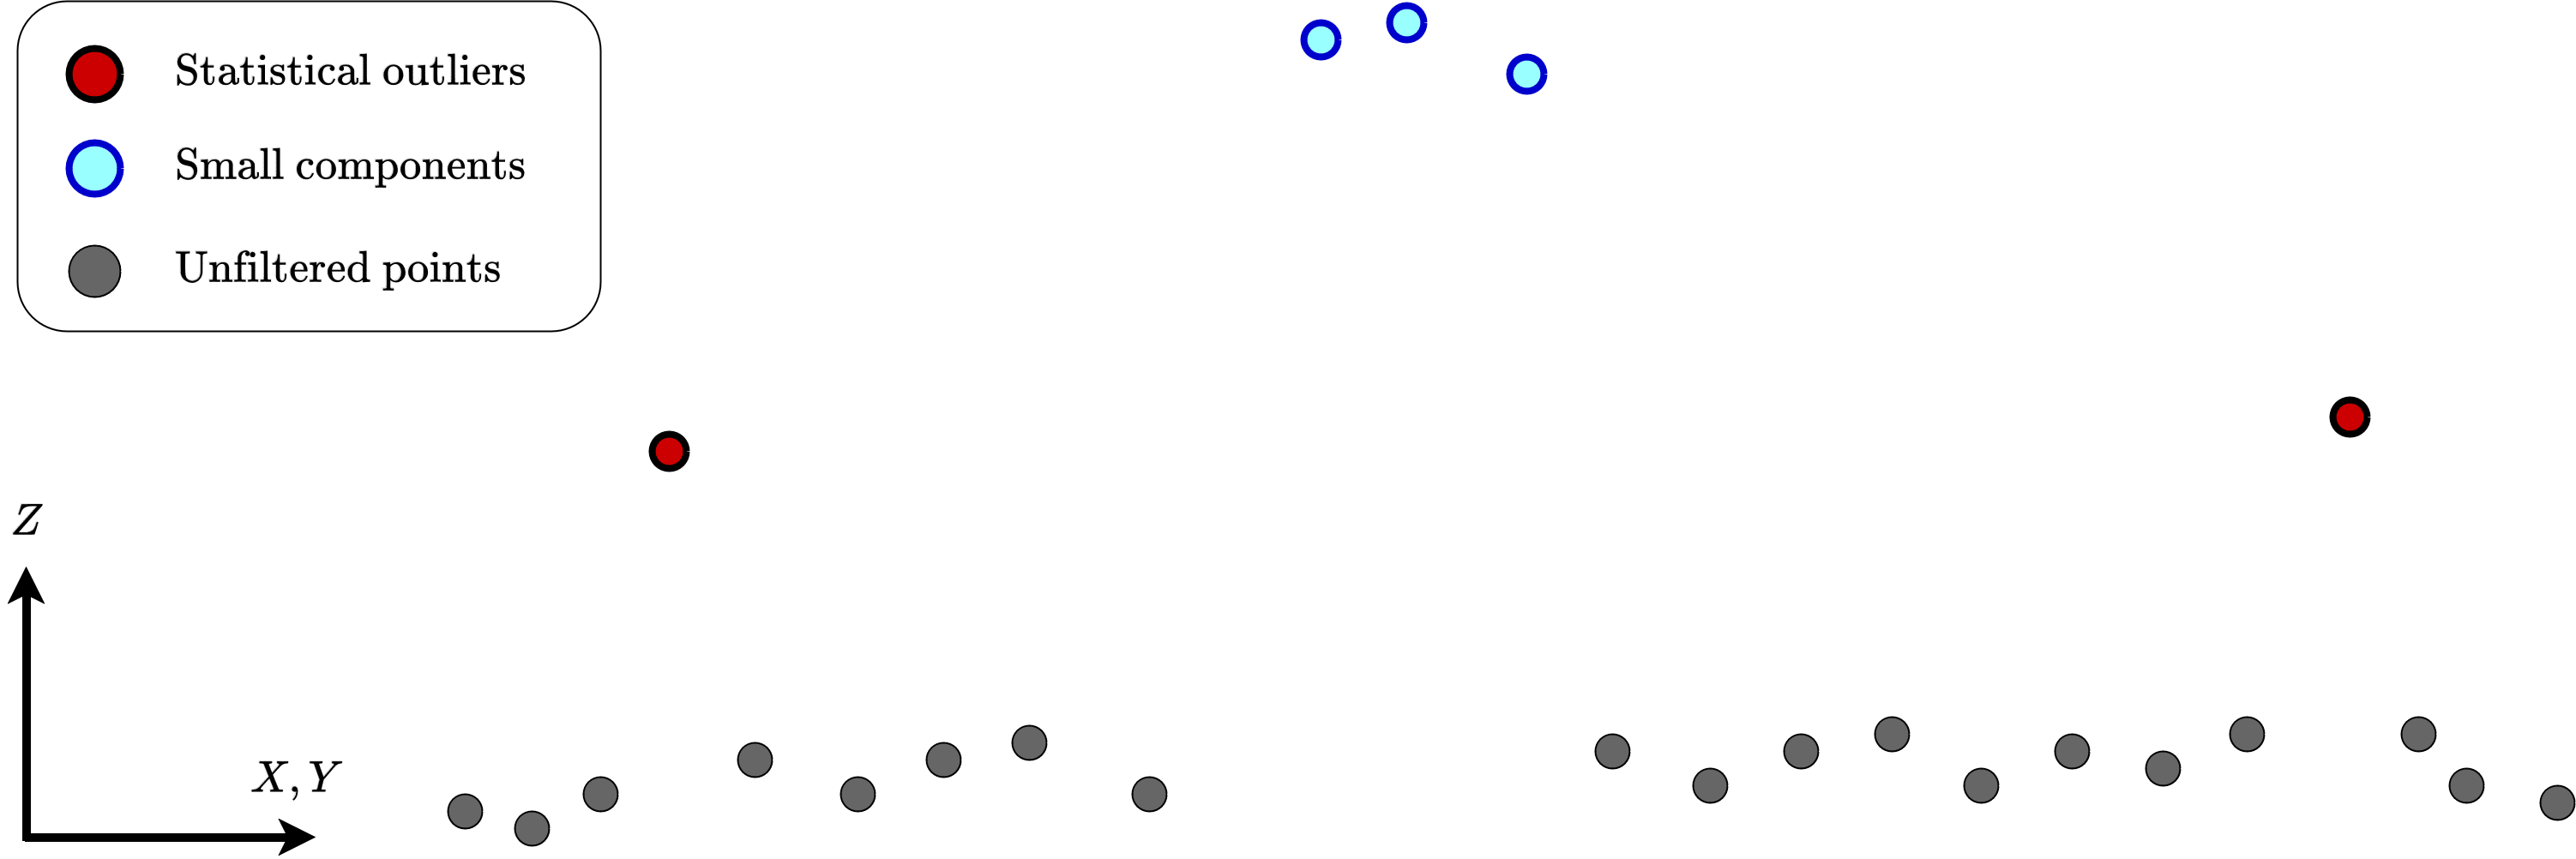
\includegraphics[width=\linewidth]{Images/Chap_1/Point_cloud_filtering.png}
    \caption{Example of statistical outliers and small components filtering of a 3D point cloud.}
    \label{fig:point_cloud_filtering}
\end{figure}

Filtering the point cloud results in a 3D product that can already be provided as such to users. However, point clouds, while containing more 3D information than DSM, can be hard to manipulate in conjunction with other \acrshort{gis} data. Projecting the point cloud on a regular grid to produce a DSM is thus often preferred, which constitutes the final step of the stereo pipeline.

\subsection{Rasterization}\label{sec:rasterization}
Rasterization consists in projecting the 3D points onto a regular grid over the $(X,Y$) plane to produce the final DSM. One of the challenges faced when projecting the point cloud is that of the relative\commanue{low?} density of the point cloud relative to the DSM grid. Indeed, if the density of the point cloud is high enough, multiple 3D points can be projected to the same cell, which raises the question on how to merge their 3D information. On the other hand, if the density is low enough\commanue{loo low?}, there may some cells where no points are projected onto. 

The CARS stereo pipeline uses a Gaussian interpolation to fuse the information of point clouds. Given a cell with coordinates $(X,Y)$ of the DSM, we consider every point $P_i=(X_i, Y_i, Z_i)$ in a given radius $r$ of $(X,Y)$, and note $\mathcal{N}_{XY}$ the set of all those points. The final value of the DSM is then computed as the following mean with Gaussian weights:
\begin{align}
    DSM(X,Y) &= \frac{\sum_{P_i\in\mathcal{N}_{XY}}Z_i\cdot e^{-\frac{(X_i-X)^2+(Y_i-Y)^2}{2\sigma^2}}}{\sum_{P_i\in\mathcal{N}_{XY}} e^{-\frac{(X_i-X)^2+(Y_i-Y)^2}{2\sigma^2}}}
\end{align}
with sigma usually set to $0.3m$ and the radius $r$ being $3m$. \Cref{fig:rasterization} illustrates the rasterization process.

Rasterizing with this method presents\commanue{provides/offers pour éviter la répétition de present} the advantage of smoothing the potential height variations still present in the 3D point cloud, while allocating more weight to points that are near the cell center. This method can also be found in other stereo pipelines \cite{shean_automated_2016}, while other pipelines use different weighting methods, such as Inverse Distance Weightings (IDW) \cite{rupnik_micmac_2017}, producing similar results.

\begin{figure}
    \centering
    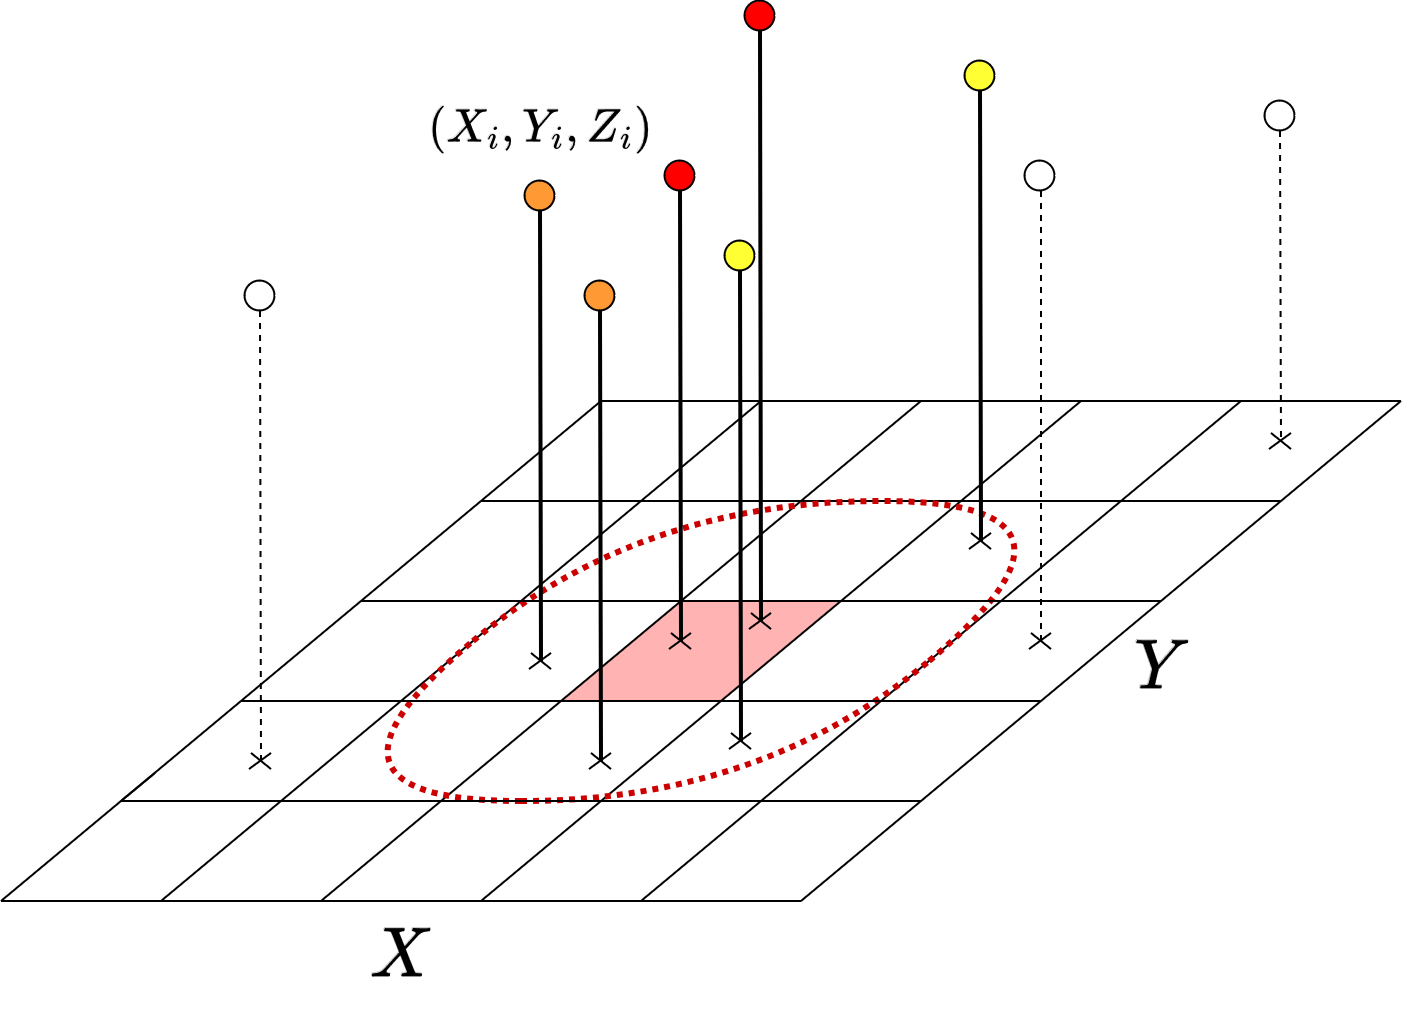
\includegraphics[width=0.7\linewidth]{Images/Chap_1/Rasterization.png}
    \caption{Rasterization of the point clouds on a regular grid. Red points are nearer to the center $(X,Y)$ of the considered cell, while yellow points are further away.}
    \label{fig:rasterization}
\end{figure}

\begin{remark}
    If no points are projected in a given cell (or its direct neighbours), then the cell can be filled with \textit{nodata} values. Different method can be considered to fill holes, such as directly using the values of nearest valid neighbouring cells, or interpolating their values. More advanced methods consists in simulating a cloth-like surface fill the holes as in \cite{lallement_bulldozer_2022}.
\end{remark}

\subsection{From LiDAR to Ground Truth Disparity}
\commanu{bizarre dans la section stereophotogrammetry pipeline. C'est plus pour la qualification. T'as vraiment besoin d'expliquer ou tu peux juste citer dans ta partie résultats quand tu abordes la qualification ? tu verras si ca saute pas du coup. Moi j'enleverais d'ici, ca n'a pas vraiment sa place, je trouve}
Parler du LiDAR HD en général. 

Explaination on how to obtain GT disparity maps from georeferenced LiDAR, \cite{cournet_ground_2020}. Line of sight and default geoid. 

\section{Uncertainty in Stereophotogrammetry}\label{sec:previous_work_stereo_uncertainty}
\todoroman{Sources d'incertitudes : acquisition des images et bruit sur le capteur. Précision du model RPC. Incertitude issue des différentes traitement (rééchantillonage, stereo matching). Intersection des lignes de visée. Rasterization.}
\commanu{du coup intro de la section à faire pour comprendre le déroulé ensuite}
\commanu{bien mettre en avant quelque part début ou fin de la section qu'il y a peu de travaux sur le sujet et que donc ton travail est novateur et défriche quelque chose de peu regardé. Remarque des implémenteurs de Mic Mac: c'est trop complexe. donc mettre quelque chose qui donne ce recul au lecteur et qui explique qu'il n'y ait pas bcp de travaux cités. Ce n'est pas un raté de ton travail d'état du lard!}
\subsection{Previous work}
\commanu{titre: on dirait que c'est ton travail précédent. Plutot state of the art?}
\todoroman{Regarder ce qui se fait sur les autres produits 3D: BD ALTI \url{https://geoservices.ign.fr/bdalti}, section 2.2.2 \url{https://geoservices.ign.fr/sites/default/files/2021-07/DC_RGEALTI_2-0.pdf}. Mission Copenicus avec WorldDEM par TandDEM X \url{https://fr.wikipedia.org/wiki/TanDEM-X}}

The quality of \acrshort{dsm} obtained using stereophotogrammetry can greatly vary depending on the quality/resolution of the images used, the precision of the geolocation, the performances of the stereo matching algorithm \etc. Reducing the magnitude of errors, or evaluating the uncertainty \textit{a posteriori} has been investigated in multiple work.
Uncertainty on \acrshort{dsm} has been mainly evaluate using a single confidence interval over the whole DSM \cite{hugonnet_uncertainty_2022, deschamps-berger_apport_2021, wang_robust_2015, oksanen_digital_2006,panagiotakis_validation_2018}. Intervals are computed based on a set of reference points, either extracted from a better resolution \acrshort{dsm}, or ground truth data. \todoroman{Reprendre le papier où ils samplent depuis leur prorpre DSM}. Fusing \acrshort{dsm} to get better accuracy \cite{qin_uncertainty-guided_2022}
\cite{hu_quantitative_2012,poggi_confidence_2021}
Deep uncertainty for disparity?

The ASP pipeline\commanu{je remettrais: The NASA's ASP pipeline cited before... } can take as inputs camera standard deviation of position uncertainty (expressed in meters) in the horizontal ground plane, and propagate it during the triangulation and rasterization steps. The documentation (\url{https://stereopipeline.readthedocs.io/en/stable/error_propagation.html}) details the covariance matrix propagation method used. It explicitly states that the propagated uncertainty does not represent the error between the predicted height and a hypothetical ground truth, even though they are expressed in the same unit of measure. It is rather the propagated covariance from the camera position projected in the horizontal and vertical directions, regardless of the matching errors or triangulation error if the line of sight do not intersect.

\subsection{Uncertainty in the CARS pipeline}\label{sec:uncertainty_cars}
In this thesis, we focused on quantifying the uncertainty alongside the creation process of \acrshort{dsm}. We thus differ in this regard from previous work, which produces a single confidence intervals from the final produced DSM. Multiple sources of uncertainty influence the production of a DSM, which we will now detail\commanu{proposition: I will now detail the multiple sources of uncertainty that influence the DSM production. remarque tjrs sur I et we, choisis et sois cohérent sur l'ensemble}.

First, the images contain noise from the captor\commanue{sensor?}, and some atmospheric effects may appear on the acquisitions. For push-broom sensors, satellite movements can have a big impact on the final images. For instance, vibration of the satellite that are not taken into account in the geometric model can lead to biases on the geolocation of the different rows of the image. Those biases will themselves be propagated to the final DSM. Those are the main uncertainties associated with the input data.\commanu{en gros tu aurais des effets sur la radiométrie (pas forcément que le bruit et l'atmosphère, ca peut etre compression ou autre artefact dans la production, je suis pas expert mais quasi sur que plein de choses...) et la géométrie (pas forcément que les vibrations, ca peut etre un mauvais calage, une mauvaise référence, je dirais qu'il y a plus que les vibrations, voir daniel). Bref, tu dois pouvoir généraliser en "radiométrie" et "géométrie" pour etre plus juste, tout en citant en exemple ce que tu as mis. A mon avis, l'analyse d'incertitude sur ces "input data" pourrait etre une thèse en soi, donc un peu court}

Other errors occur when processing this data. First, different resampling\commanue{several resamplings?} occur in order to convert stereo images from captor\commanue{alors captor je ne suis pas fan je mettrais sensor} geometry to epipolar geometry. Those resamplings introduce errors if the input and target resolutions do not respect Shannon criteria \cite{delon_small_2007} \todoroman{mettre les formules? affiner la phrase}. Moreover, the sparse matches used to refine the epipolar grid heavily\commanue{strongly?} depend on the performance of the SIFT algorithm used to obtain them. In similar terrain, for instance on glaciers where many homogeneous region are present, some false matches can be observed. This leads to wrong epipolar lines, and those errors will themselves be propagated in the following steps of the pipeline\commanue{Oui on a aussi un problème sur des champs où l'alignement n'était pas bon. Après je pense que c'est surtout qu'avec les SIFTS parfois on trouve pas le bon intervalle...}. Those errors are usually minor, compared to those occurring in the dense stereo matching step\commanue{Ah bah voilà c'est forcément la faute de pandora. David et Dimitri ont trop déteint sur toi ;)}.

Dense stereo matching is a complex task, for which many different algorithms exist, each potentially presenting different performances. Using a window-based correlator with SGM regularization usually presents good performance in areas without height discontinuities. This can become a problem in urban areas, where the presence of high buildings represents an additional challenge for the correlator. Because the correlator compares windows ($5\times5$ using the CENSUS cost function or $11\times11$ using MC-CNN) and not single pixels, this naturally creates an adherence effect near building borders\commanue{Alors moi j'ai lu les différentes versions de ce chapitre donc là il faut peur-être faire un renvoi à l'adhérence}. Note that in \cite{okutomi_stereo_1994}, authors have been trying to adapt the window shape to reduce the uncertainty of stereo matching, but this method requires to iteratively compute costs on different windows, which can become quite expensive. SGM regularization also penalizes disparity changes, thus reinforcing the adherence effect. Other processes, such as filtering or sub-pixel refinement, improve the quality of the disparity map but require specific care for handling their induced uncertainty. Sub-pixel refinement also supposes that sub-pixel disparities can be deducted without upsampling the input images, which is debatable\commanue{C'est plutôt qu'on ne vérifie pas que la fonction de coût est suffismament échantillonnée et effectivement si ce n'était pas le cas il faudrait suréchantillonner l'image, là tu me fais un peu la version raccourcie}. The dense matching step is crucial as previous errors usually have a smaller impact on the final product than the errors potentially occurring in stereo-matching\commanue{Même si la phrase me rend triste il faudrait la mettre en début du paragraphe, elle est importante et te fera le lien avec avant. D'ailleurs tu peux mettre aussi le reste du paragraphe avant.}. For instance, a bias in the epipolar grid typically leads to a shift of one row between the epipolar images. This leads to typical errors of around $1$ disparity. In comparison, the correlator can produce errors with a magnitude of the whole disparity research interval, sometimes reaching values near $100$ disparities. Considering those orders of magnitude, estimating and quantifying the uncertainty of the stereo-matching process is crucial to control the uncertainty on the output DSM. \Cref{sec:uncertainty_pandora} dives more into details regarding the different methods that have been developed to quantify the uncertainty of dense stereo matching.

Once the disparity has been estimated, 3D points can be triangulated by intersecting RPC lines from each matched pixel. However, we saw previously that there is no guarantee that the 3D lines do intersect. If they indeed do not intersect, the 3D point is defined as the point minimizing its squared distances to both lines of sight. An alternative is to modify the geolocation line from the secondary image so as it intersects the line from the reference image. In both cases, the localization of the 3D point is not exact. This uncertainty stems from the fact that we determine the 3D coordinates of the point from a match between two pixels that do not point exactly to the same object\commanue{Je comprends ce que tu veux dire mais il faudrait voir si on peut pas améliorer la formulation. Avec l'échantillonnage des pixels les pixels ne sont pas exactement comparable. Je réfléchis à comment le reformuler}. Additionally, RPC models attempt to represent real lines of sight with polynomial coefficient, which is not exact and possess its own accuracy. The method used for coefficients calibration and the frequency of calibration also bring their share of uncertainty.

The final part of the stereo pipeline is to rasterize the point cloud onto a regular grid, thus yielding the DSM. When characterizing the uncertainty on the final result, we must first agree on what the DSM is supposed to represent. It is common to consider that each pixel's value should represent the average height over the cell. However, providing the maximum or minimal height might be more adapted to some scenarios: for instance if the DSM is used to prepare very low altitude flights (for drones \etc), the maximum height is more relevant as one would want to avoid any foliage or power line. Those elements could disappear in the fin\commanue{clairement il manque la fin ;)}. In this thesis, we will consider that the DSM represents the (weighted) average height. The weights considered will be computed with a Gaussian whose variable is the distance to the center of the cell\commanue{Remarque un peu globale mise à l'arrache ici, mais il faudrait relire quand tu auras fini la partie d'avant pour voir si ça ne fait pas trop redite avec la description du pipeline}. Other weights can be considered, most notably the \textit{inverse distance weighting} (IDW), which produces very similar results in our applications. We now specified the projection method\commanue{Pourquoi au passé?}. Depending of the resolution of input images and the desired output resolution of the DSM, the density of points per DSM cell will vary. In our applications, the input and output resolutions are identical as we typically desire to produce a DSM at $50$cm resolution from $50$cm panchromatic images. This means that there is on average one 3D point per DSM cell. For occluded regions, or when we discarded stereo matches that seemed wrong, there might be no point directly in the output cell. In this case, the value of the DSM cell will be completely determined by the value of points in neighbouring cells, even if their distance is high and the averaging weights are small. Interpreting the final DSM as the average height on each cell is thus debatable, as the average is computed on a limited number of points, and sometimes not even belonging to the considered cell.  Note that if there is no points around in a given radius, the cell will be left empty. 

Different sources of uncertainty occurring throughout the stereo pipeline were presented in the previous paragraphs. Characterizing, modelling and propagating all of those uncertainties could not be considered in the span of this thesis. We thus focus mostly on the uncertainty arising from the dense stereo matching step, as it is the source of the biggest errors in the pipeline. \Cref{chap:propagating} investigates how uncertainty from the input epipolar images can be propagated in the stereo matching step, and \Cref{chap:epistemic_uncertainty} attempts to model the processing uncertainty of stereo algorithm itself. We also propagate this uncertainty all the way to the output DSM and show that it can correctly estimate the errors made during the DSM production. 

We conclude this section with a small disclaimer: our methodology estimates the uncertainty independently for every pixels, leading to small confidence intervals in confident areas, and bigger confidence intervals where the algorithms may have performed badly. We differ in this regard to the methods presented in \Cref{sec:previous_work_stereo_uncertainty}, which estimate a single global confidence interval \textit{a posteriori}, based solely on the DSM (and reference points), regardless of the method used to obtain it. In this regard, it does not seem relevant to compare our intervals to theirs, as there most similar characteristics is their name ``interval'', but neither share the same form (single \vs multiple intervals), nor are based on the same data. \commanu{je me demande si tu peux pas mettre cette dernière partie dans une sous section à part. Ce ne serait donc pas un disclaimer mais une présentation  Cette sous section (et la suivante sur le dense matching) décrit les sources d'incertitude que tu vois et pourrait amener à une sous section de transition ou tu expliques et justifies les choix pris pour la thèse vers le chap 4 et 5 en disant que l'idée était de prendre aussi les techniques méthodologiques du chap 2 et 3 en considération. }

\subsection{Uncertainty Quantification in Dense Stereo Matching}\label{sec:uncertainty_pandora}
As stereo-matching is a popular problem in computer vision, many methods for quantifying its uncertainty have been proposed in the literature. Without being exhaustive, this section presents a quick overview of the main approaches as well as the solutions currently implemented in the dense stereo correlator Pandora used in the CARS pipeline.

The way uncertainty is quantified in stereo matching is by producing \textit{confidence maps}, \ie a mapping for each pixel $(row, ~col)$ to a real confidence value, usually between $0$ and $1$. By convention, a value of $0$ means that we are not confident in the disparity value associated to $(row, ~col)$. Conversely, a confidence value of $1$ indicates that we are very confidence in the predicted disparity.

\begin{remark}
    \todoroman{Faire relire cette remarque à Manue et Seb car je l'ai écrite après leur relecture }It is interesting to see that in \cite{quinio_random_1992}, the author considered using closed random sets (a concept related to imprecise probabilities and belief functions studied in \cref{chap:representation_of_uncertainty} \cite{quinio_random_1991}) to model the uncertainty of a stereoscopic setup. They mainly consider the uncertainty arsing from the limited resolution of digital images (as we do in \cref{chap:propagating}), and from the precision of the calibration setup: focal length of cameras, baseline distance, orientation and vengeance angle of the cameras \etc. They consider that the uncertainty from dense matching is not of epistemic nature, but of aleatoric nature, and thus do not model it by imprecise models as we do in \Cref{chap:epistemic_uncertainty}. This hypothesis is justified as they achieve the stereo matching step using a window based ZNCC cost function (without \acrshort{sgm}, as it was not published at the time), which by nature possess strong links with probabilistic models.
\end{remark}

There are multiple sources of information that can be used to compute a confidence measure. Left and right input images and the predicted disparity map being those available to every method, but cost-based approaches can also make use of the cost volume, as it contains a lot of useful information. Most confidence measures were first handcrafted using those different information sources. For reviews on those methods, we refer to \cite{egnal_stereo_2004, hu_quantitative_2012, poggi_quantitative_2017}. With the rising use of deep-learning in stereo, many networks have been developed to estimate the uncertainty. A review for methods using regression forests can be found in \cite{min-gyu_park_leveraging_2015}, and a more general review, including the use 2D and 3D CNNs on the cost volume, can be found in \cite{poggi_confidence_2021}.

\begin{remark}
     Quantifying the uncertainty in stereo matching is a popular field of research. Recently, people have even been trying to evaluate the uncertainty of the confidence estimation itself, called \textit{meta-confidence} \cite{kim_meta-confidence_2022}.
\end{remark}

\begin{example}
    Let us present some examples of confidence measures that use different sources of information.\commanue{Pourquoi tu ne mets pas cette phrase à l'extérieur de l'encart, afin de ne pas avoir l'encart qui poppe. Après je ne sais pas au final si un encart est nécessaire.}
    
    Regarding confidence measure based on the disparity map, we already presented a type of binary confidence measure in \Cref{sec:postprocess_disparity} with the cross-checking test from \cref{eq:cross-checking}. Other methods compute for instance the local variance of the disparity map, where a low variance suggests confident regions.
    
    For methods using the cost volume, a simple method for measuring the cost would be using the value of the matching score measure (MSM, \cite{egnal_stereo_2004}) for a given disparity at coordinates $(row, ~col)$:
    \begin{equation}
        MSM(row, ~col) = -C_V(row, col, \mathcal{D}(row, ~col))
    \end{equation}
    This measure can be normalized between $0$ and $1$ using the global minimum and maximum of the cost volume. The idea behind this measure is the following: a high matching cost for a selected disparity indicates that the two matched pixels are not that similar, and thus the match is not confident. Other measures using the matching cost compare the value of the first and second minimum of a cost curve, or measure the curvature of the cost curves. More advances measures make use of 3D CNNs on the entirety of the cost volume to learn an efficient confidence measure \cite{mehltretter_cnn-based_2019}.
    
    Measures based on the input images usually measure the gradient \cite{haeusler_ensemble_2013} or variance \cite{park_learning_2019} of input images. High gradient or high variances indicate highly-textured regions, which are often easier to match. The confidence is therefore higher for those pixels. 
    
    Deep-learning approaches can combine multiple sources of information (input images, cost volume, disparity map) to learn a confidence measure \cite{tosi_beyond_2018, kim_adversarial_2020}.
\end{example}

In this thesis, we will also consider three confidence measures that can already be computed with our correlator. Those measures will help us to quantify the uncertainty in the photogrammetry pipeline or will be used as comparison with our proposed method.

\begin{figure}
    \centering
    \begin{subfigure}[t]{0.5\linewidth}
        \centering
        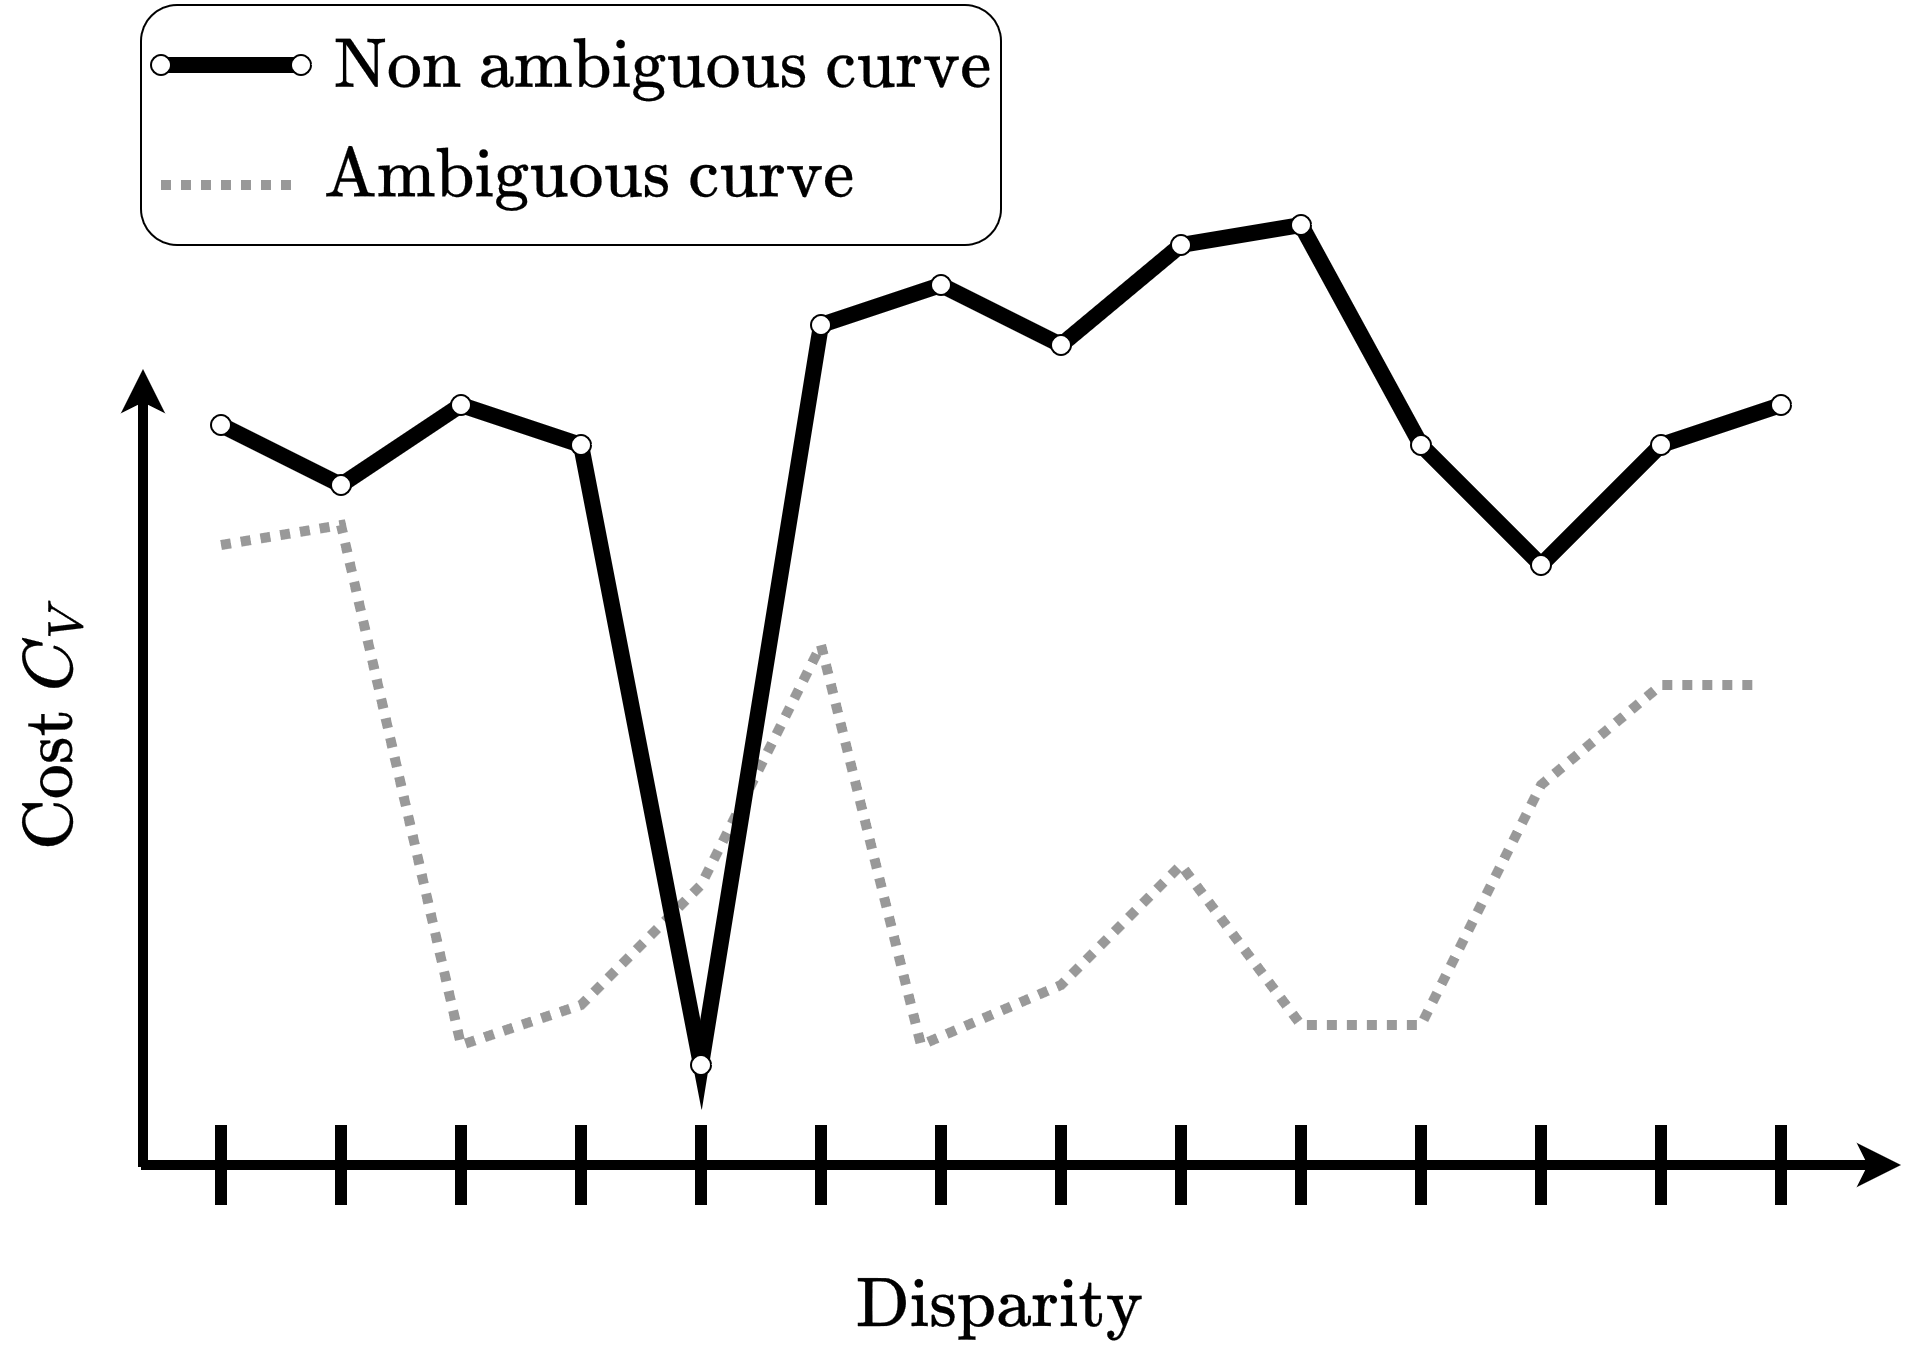
\includegraphics[width=\linewidth]{Images/Chap_1/Ambiguity.png}
        \caption{}
        \label{fig:ambgiuity}
    \end{subfigure}\hfill
    \begin{subfigure}[t]{0.5\linewidth}
        \centering
        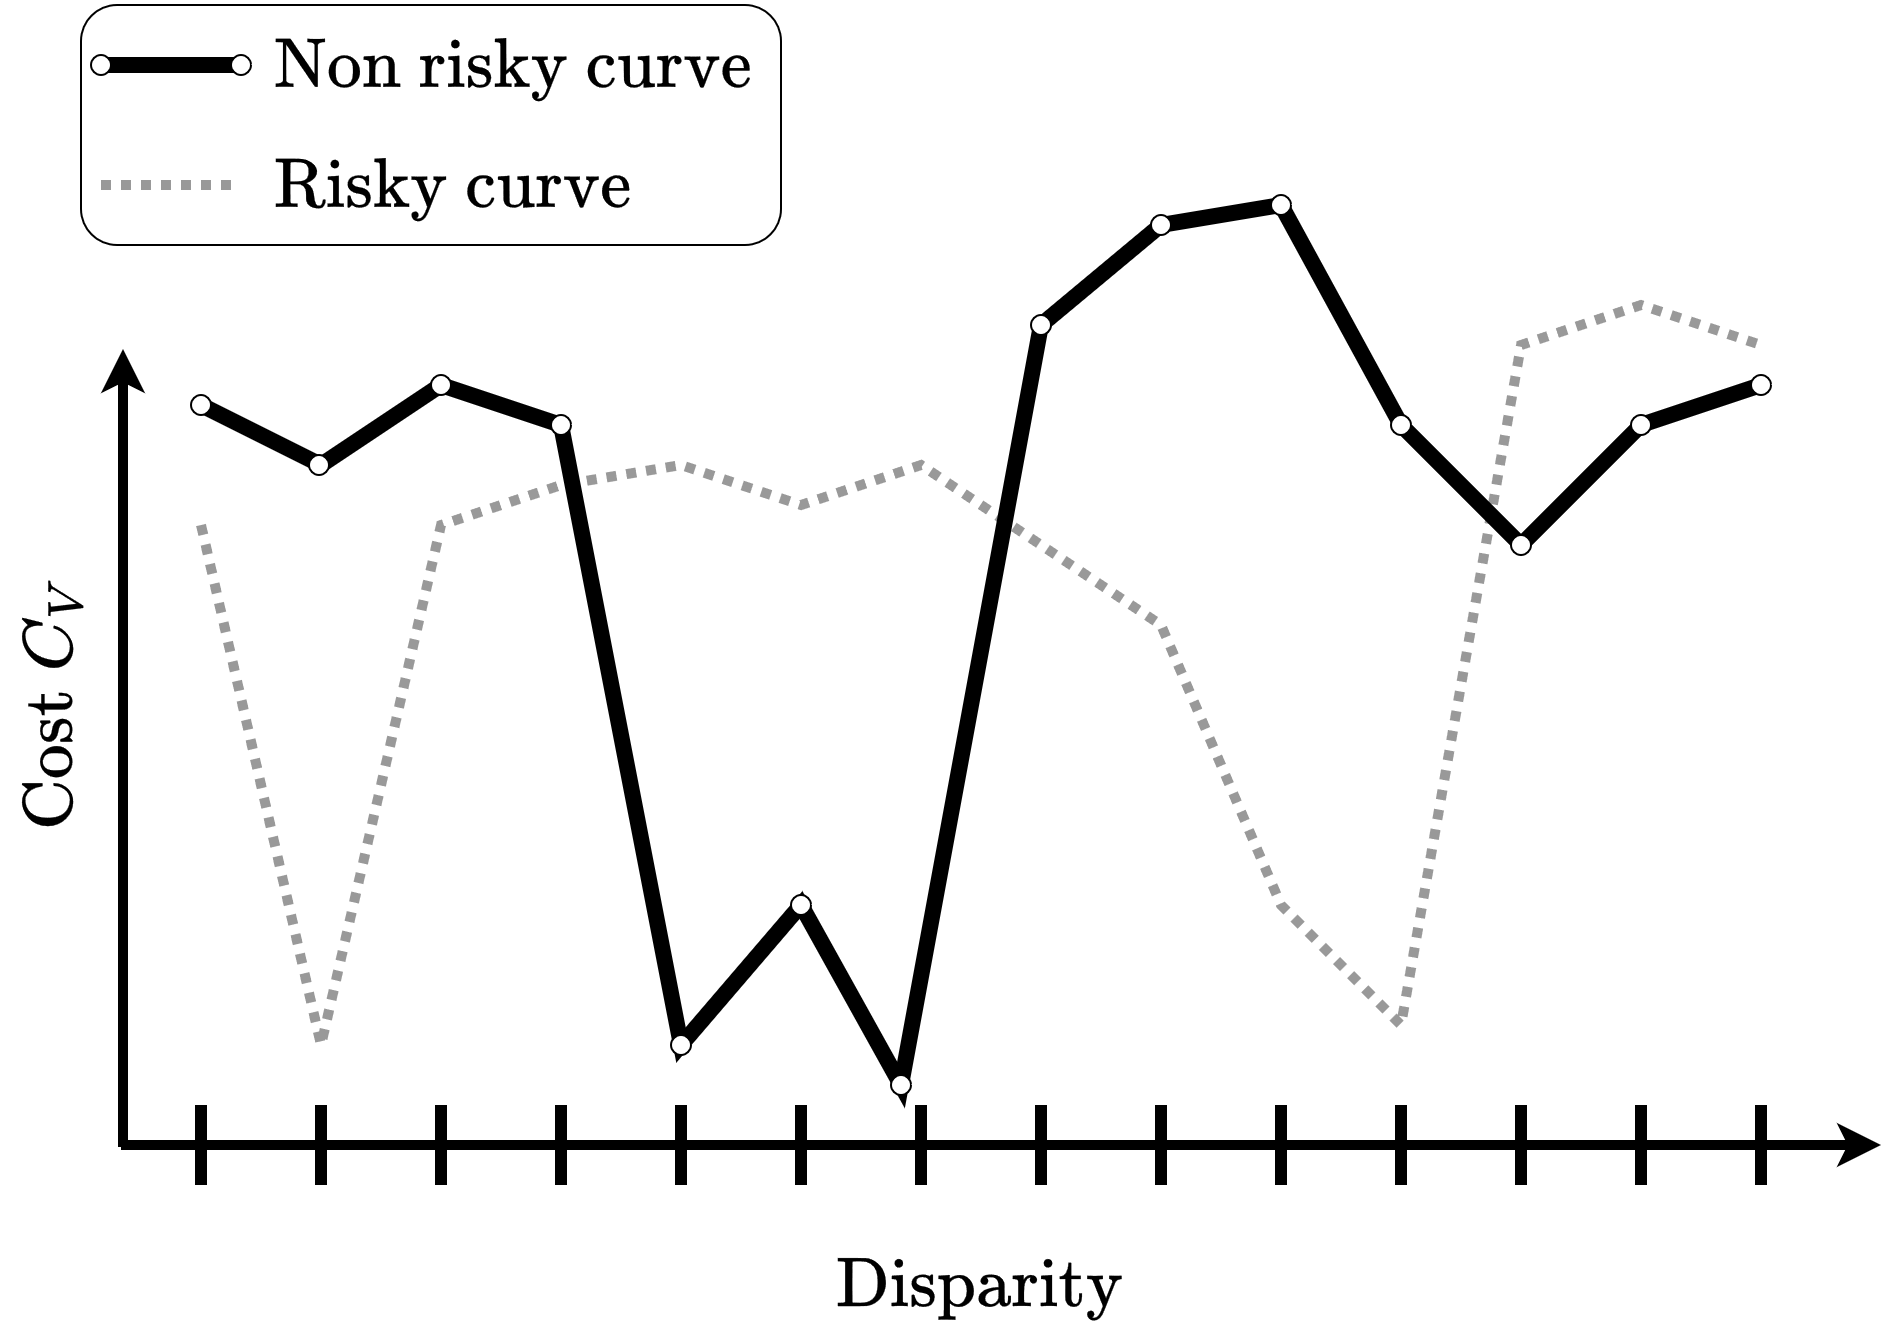
\includegraphics[width=\linewidth]{Images/Chap_1/Risk.png}
        \caption{}
        \label{fig:risk}
    \end{subfigure}\hfill
    \caption{Cost curves with different levels of ambiguity \ref{fig:ambgiuity} and risk \ref{fig:risk}}
    \label{fig:ambiguity_risk}
\end{figure}

The first confidence measure is a confidence measure called \textit{confidence from ambiguity} \cite{sarrazin_ambiguity_2021}. This method is based on the cost volume and quantifies how easy or hard it is to single out the correct disparity in a cost curve. \Cref{fig:ambgiuity} presents two curves: one that is ambiguous and one that is not\commanue{Alors tu as une phrase qui reprend cette info en la complétant donc cette phrase est en trop.}. To compute it, we first start by constructing what is called an \textit{ambiguity curve}. We do that by counting how many disparities have a cost close within a threshold $\eta$ to the minimal cost, for increasing values of $\eta$. \Cref{fig:ambgiuity} presents two cost curves, one which is not ambiguous as there is a single well defined minimum, and an ambiguous cost curve which presents multiple values that are close to the minimum. Formally we need to define for a pixel $(row, ~col)$ the set of all disparities whose cost is within a range $\eta$ of the minimal cost, and then define the ambiguity curve as the cardinal of this set:
\begin{align}
    &\mathcal{D}_\eta = \{d ~|~ C_V(row,~col,~d) \leqslant \min_\delta C_V(row, ~col, ~\delta) + \eta\}\\
    &Amb(row, ~col, ~\eta) = \#\mathcal{D}_\eta
\end{align}
where $\#$ is the cardinal of a set. Evaluating $Amb$ for different $\eta$ gives the ambiguity curve. \Cref{fig:integral_ambiguity_1} presents a cost curve with different values of $\eta$. \Cref{fig:integral_ambiguity_2} presents the resulting ambiguity curve. On those two figures we can see for instance that for $\eta_3$ there are $6$ disparities whose cost is lower than $\min_\delta C_V(row, ~col, ~\delta) + \eta_3$. For non-ambiguous cost curves, $Amb$ will increase only for high values of $\eta$. On the contrary, for ambiguous curves, $Amb$ will be high for small values of $\eta$. To obtain a scalar value from $Amb$, we compute the area under its curve, normalized by the range of $\eta$:
\begin{equation}
    \mathrm{AUC}_{Amb}(row, ~col) = \frac{1}{\max\eta-\min\eta}\int_\eta Amb(row,~col,~\eta)d\eta
\end{equation}
However, this results on low values for confident (non-ambiguous) cost curves, and high values for less confident (ambiguous) curves. The confidence from ambiguity $c_{Amb}$ is thus obtained by normalizing and reverting the integral:
\begin{equation}\label{eq:confidence_from_ambiguity}
    c_{Amb}(row, ~col) = \frac{\max \mathrm{AUC}_{Amb}- \mathrm{AUC}_{Amb}(row, ~col)}{\max \mathrm{AUC}_{Amb} -\min \mathrm{AUC}_{Amb}}
\end{equation}
This way, values of $c_{Amb}$ near $0$ indicate that we are not confident in the predicted disparity. Reversely, values of $c_{Amb}$ near $1$ indicate that we are confident in the predicted disparity.

\begin{figure}
    \centering
    \begin{subfigure}[t]{0.6\linewidth}
        \centering
        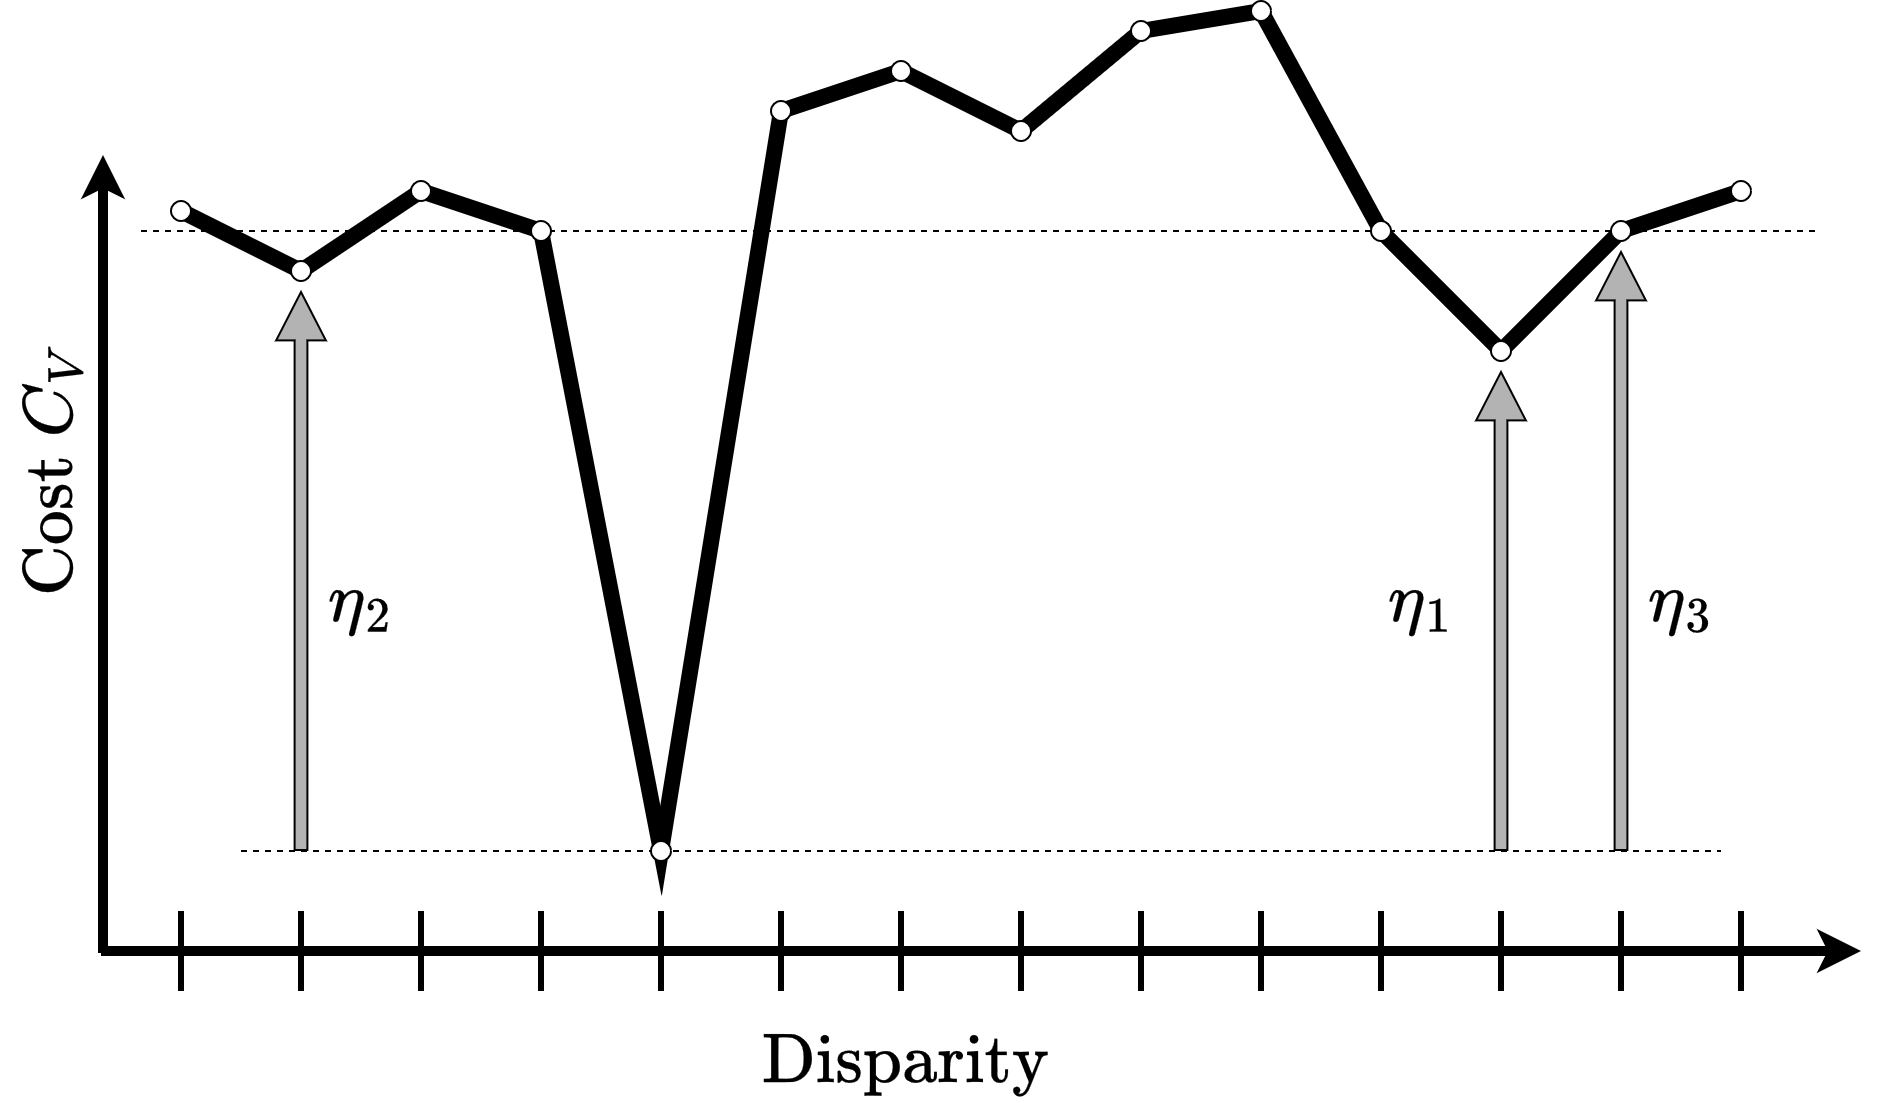
\includegraphics[width=\linewidth]{Images/Chap_1/Integral_Ambiguity_1.png}
        \caption{Cost curve with different values of $\eta$. Horizontal dotted lines indicates the range of costs between $\min_\delta C_V(row, ~col, ~\delta)$ and $\min_\delta C_V(row, ~col, ~\delta)+\eta_3$}
        \label{fig:integral_ambiguity_1}
    \end{subfigure}\hfill
    \begin{subfigure}[t]{0.4\linewidth}
        \centering
        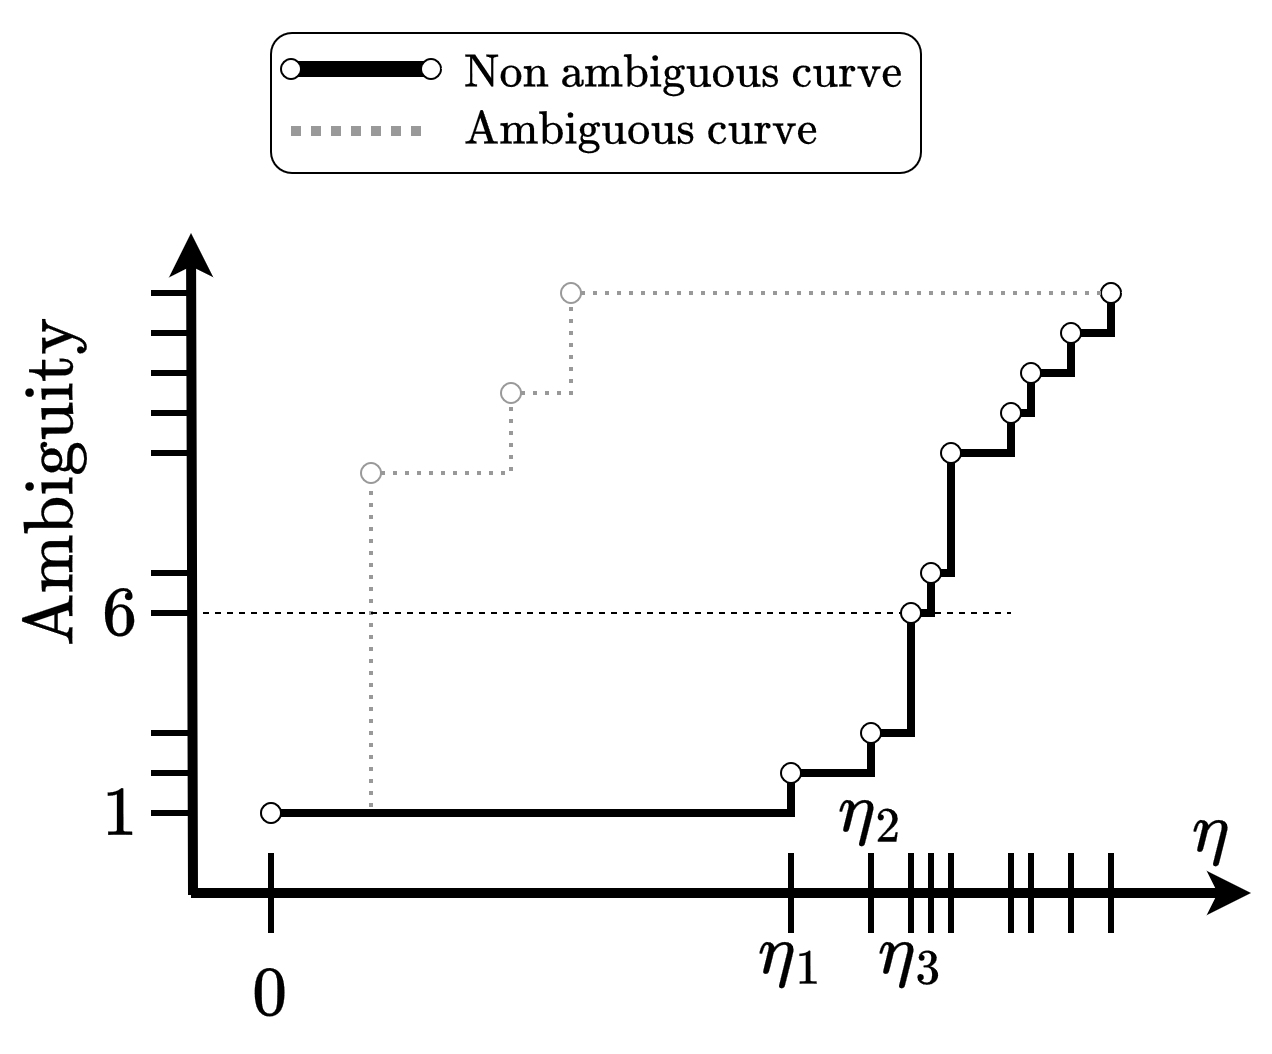
\includegraphics[width=\linewidth]{Images/Chap_1/Integral_Ambiguity_2.png}
        \caption{Associated ambiguity curve in full line. Ambiguous curve in gray dotted line}
        \label{fig:integral_ambiguity_2}
    \end{subfigure}\hfill
    \caption{Illustration of the computation of the ambiguity curve.}
    \label{fig:integral_ambiguity}
\end{figure}

The second confidence measure that we consider is named \textit{confidence from risk}. It is designed to measure if the magnitude of a potential error is high or low. After all, if we predict a wrong disparity while the correct disparity is right next to our prediction, the impact on the final result will be smaller than if the true disparity is at the other side of the disparity range. Keeping this in mind, we apply the same methodology as for the ambiguity. We consider the set $\mathcal{D}_\eta$ of all disparities whose cost is less than $\eta$ away from the minimal cost, and define the risk as the gap between extrema of this set:
\begin{equation}
    R(row, ~col, ~\eta) = \max_{\mathcal{D}_\eta}d - \min_{\mathcal{D}_\eta}d
\end{equation}
\Cref{fig:integral_risk_1} presents a cost curve with different values of $\eta$ and their associated risk $R$. \Cref{fig:integral_risk_2} presents the resulting risk for all $\eta$. For non-risky cost curves, $R$ will increase only for high values of $\eta$. On the contrary, for risky curves, $R$ will be high for small values of $\eta$. To obtain a single scalar, we compute the area under the risk curve, normalized by the range of $\eta$:
\begin{equation}
    \mathrm{AUC}_R = \frac{1}{\max\eta-\min\eta}\int_\eta R(row,~col,~\eta)d\eta
\end{equation}
$\mathrm{AUC}_R$ is thus expressed in number of disparities. Contrary to the confidence from ambiguity, the risk is kept as such with its current unity. 

\begin{remark}
     The risk measures the magnitude of the potential error, but not its probability. It is therefore possible to have a very risky cost curve, but which is not ambiguous at all. In other words, it means that the probability of an error occurring can be very low, but if it somehow happened, then the magnitude of this error would also be very low. The risk is thus a confidence measure that need to be completed by a measure such as ambiguity. On it own, it has less meaning than other measures.
     
    \begin{comment}
        As detailed in \Cref{sec:co3d}, one of the requirements of the CO3D mission is to produce a performance map associated with the output DSM, expressed in meters. In order to produce such a performance map, one of the leads explored at CNES was to combine the confidence from ambiguity and the risk. This is done by weighting the risk with $1-c_{Amb}$, so as to reduce the risk of confident pixels. The result, expressed in number of disparities, can itself be converted into meters using the disparity to altitude ratio $d_{alt}$ computed along epipolar grids (see \Cref{sec:epipolar_geometry}). Finally, internal studies using real data have concluded that a good candidate for a performance criterion was:
        \begin{equation}
            perf(row, ~col) = \min(1, ~\frac{1-c_{amb}(row,~col)}{\tau_{amb}})\cdot \mathrm{AUC}_R(row,~col) \cdot d_{alt}
        \end{equation}
        where $\tau_{amb}$ is a threshold usually set to $0.4$. In plain words, if the confidence from ambiguity drops below $1-\tau_{amb}$, then we do not use the ambiguity weighting and the performance equals $\mathrm{AUC}_R \cdot d_{alt}$. This performance criterion thus provide a confidence measure expressed in meters, associated to a 3D point, which can then be rasterized alongside the DSM to produce the desired performance map. We will use it as a comparison for our method in \Cref{chap:epistemic_uncertainty}.
    \end{comment}
\end{remark}

\todoroman{Dire qu'il y a eu des tentatives internes pour allier risk et amb pour faire une carte de perf. Nos travaux s'inscrivent dans cette continuité pour proposer une autre méthode. Il est envisagé de peut être l'utiliser dans la chaine CO3D.}

\begin{figure}
    \centering
    \begin{subfigure}[t]{0.6\linewidth}
        \centering
        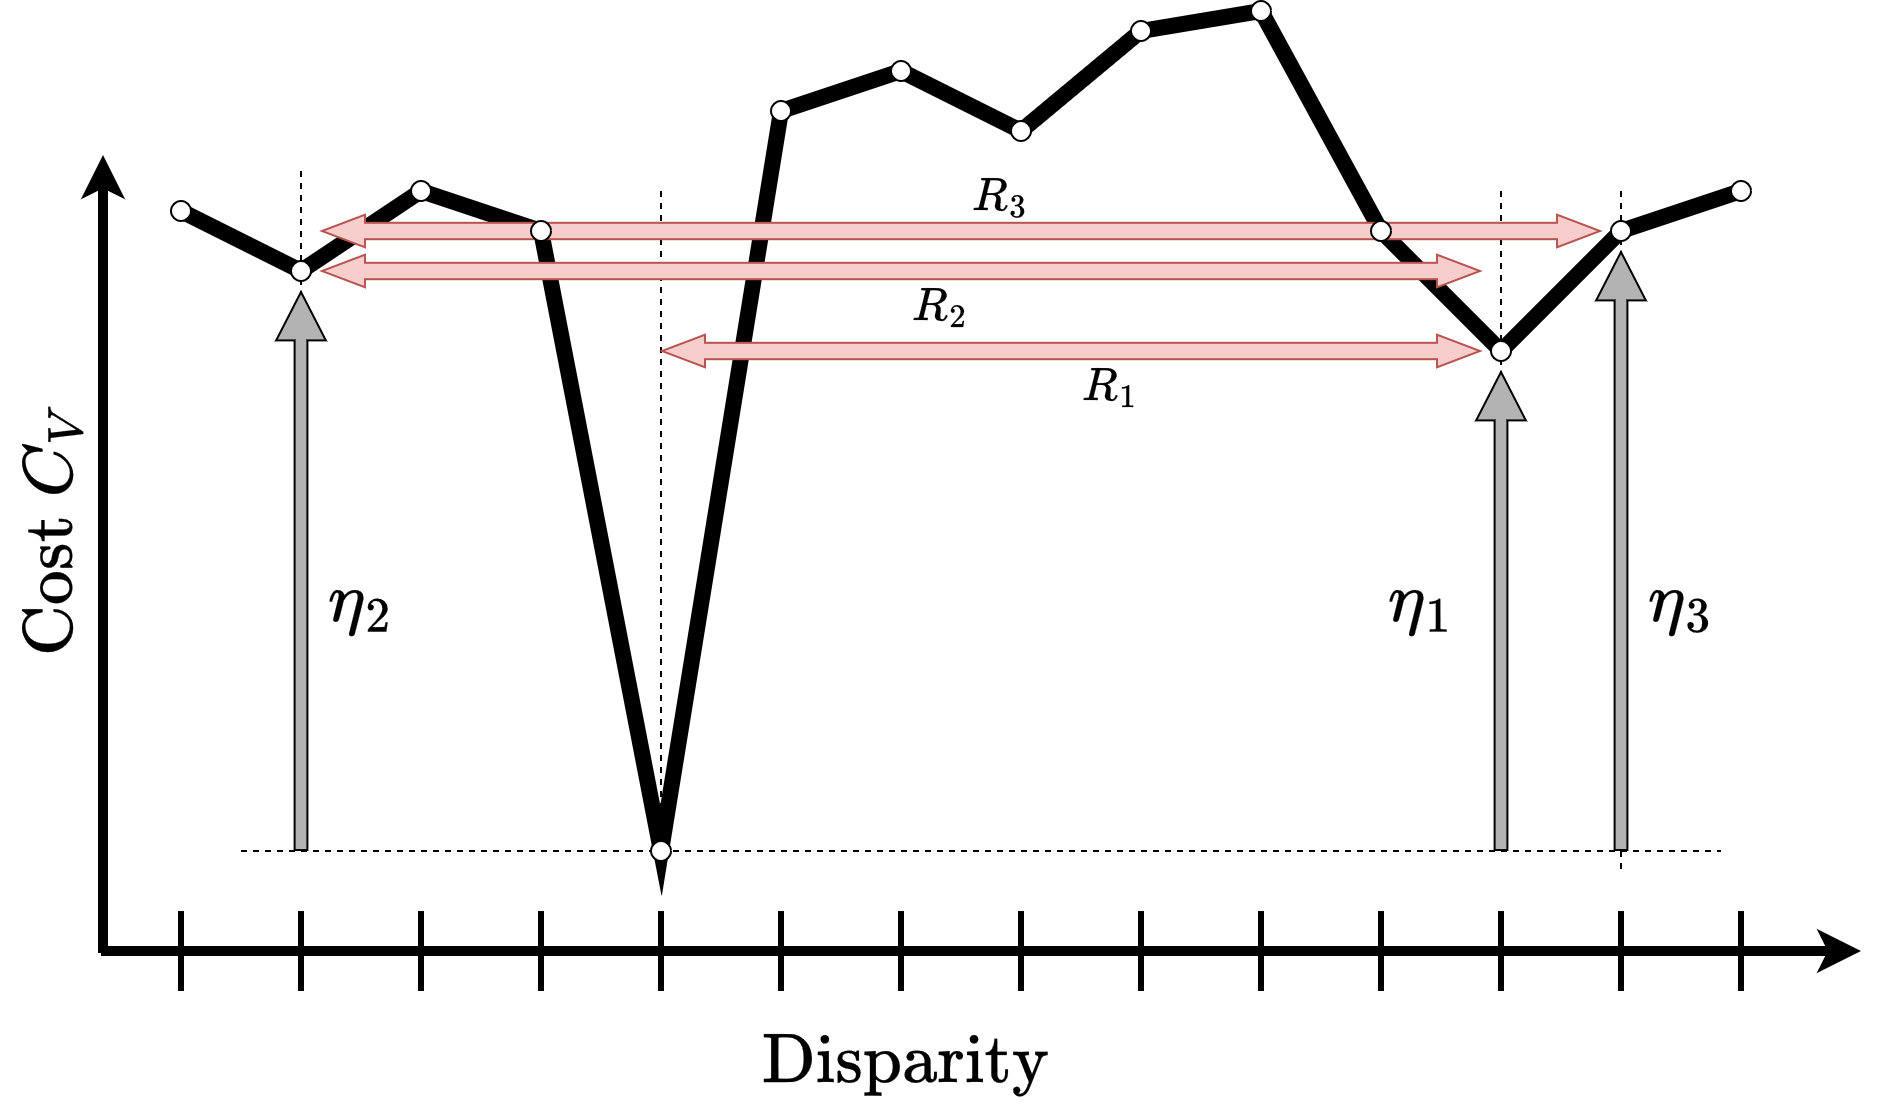
\includegraphics[width=\linewidth]{Images/Chap_1/Integral_Risk_1.png}
        \caption{Cost curve with different values of $\eta$ and risk}
        \label{fig:integral_risk_1}
    \end{subfigure}\hfill
    \begin{subfigure}[t]{0.4\linewidth}
        \centering
        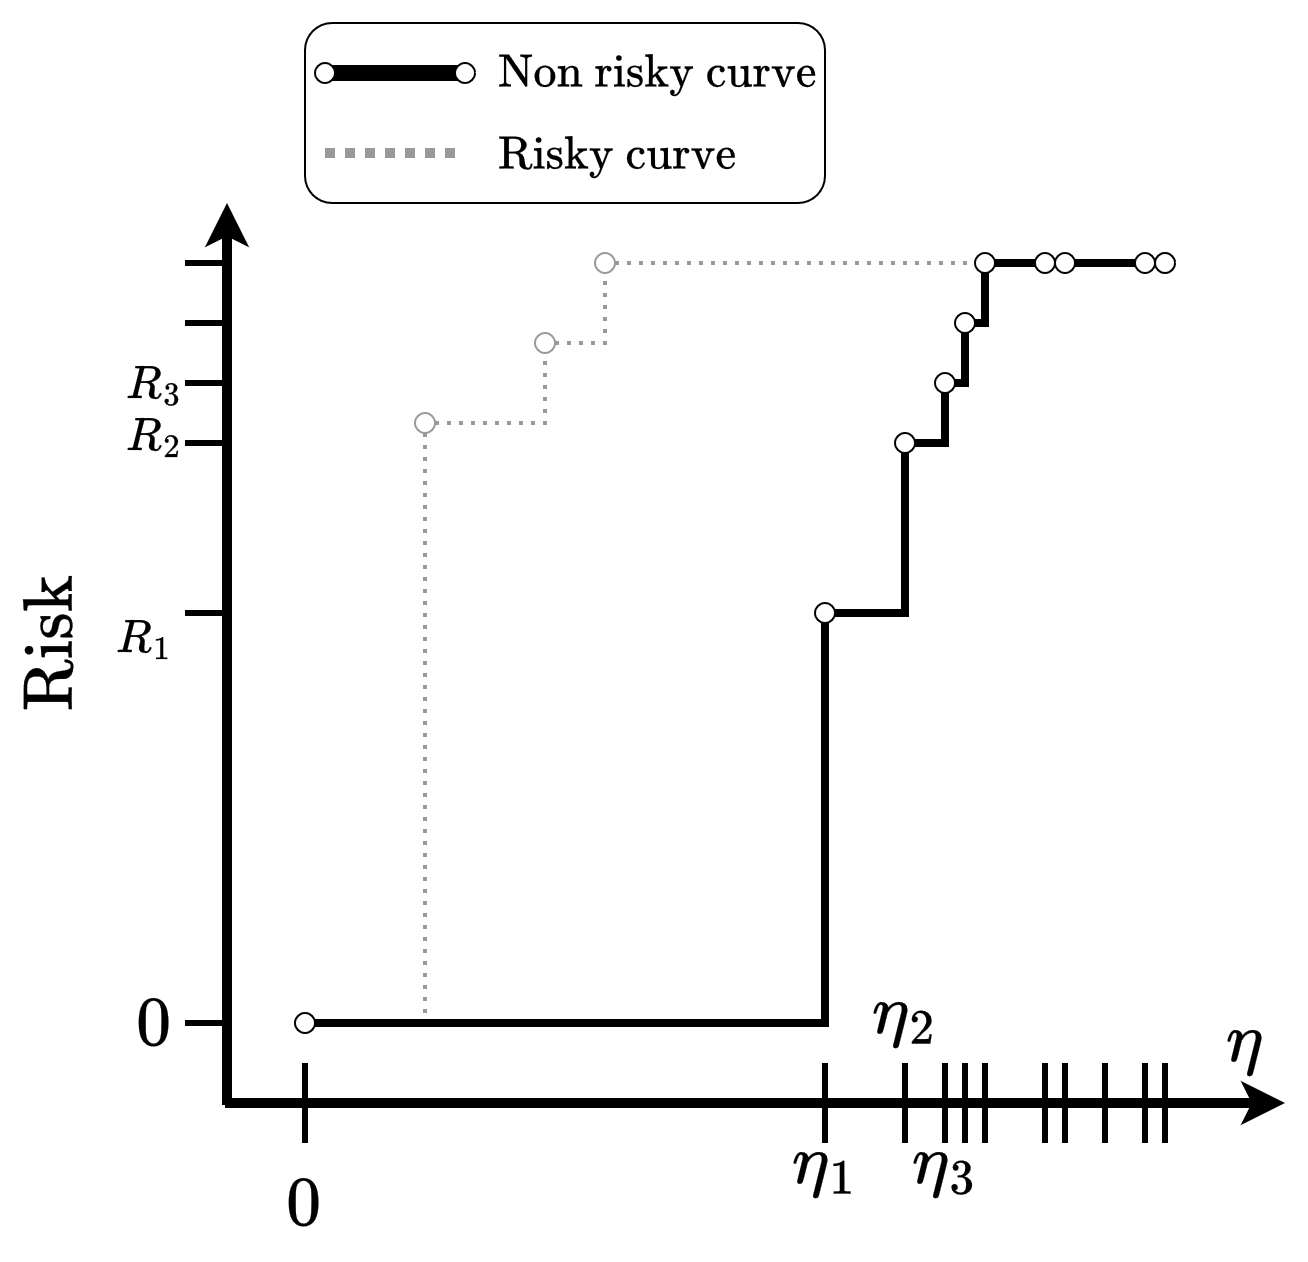
\includegraphics[width=\linewidth]{Images/Chap_1/Integral_Risk_2.png}
        \caption{Associated risk curve in full line. Risky curve in gray dotted line}
        \label{fig:integral_risk_2}
    \end{subfigure}\hfill
    \caption{Illustration of the computation of the risk curve.}
    \label{fig:integral_risk}
\end{figure}

\commanue{pas de conclusion ? en même temps tu reste constant avec tes principes}
\pagebreak
\blankpage

    
    \setkeys{Gin}{draft=true}
    \chapter{Mathematical Representations of Uncertainty}\label{chap:representation_of_uncertainty}

\section{Introduction}
This chapter takes some distance from the stereo vision problem presented previously, and instead describe more formally different representations of uncertainty and the tools that can be used to manipulate them. In this thesis, we consider classical probabilities (\Cref{sec:probabilities}), possibility distributions (\Cref{sec:possibilities}) and p-boxes (secction \ref{sec:pboxes}) to model uncertainty. We also consider the case where we consider multiple sources of uncertainty simultaneously. In this setting, the dependency between the different sources must be taken into account. We thus present a dependency model called copulas in \Cref{sec:copulas}, and some of its properties. The thorough presentation of those concepts will then be put into relations in \Cref{chap:joining_credal_sets}. 

\section{Notations}
We introduce here a few notations that will be used in the rest of this chapter. \todoroman{A ajouter au fur et à mesure, peut être déplacer au début de la thèse, à côté du glossaire.} \commanu{en effet, pas mal à coté du glossaire, mais garder une phrase avec un lien pour aller les chercher si besoin pour le lecteur. sinon pas sur de l'anglais pour 'the rest of this chapter', ca sonne très francais, j'enleverais. Plus simple: I (ou we mais idem pareil) introduce here... will be used in this chapter. }
\begin{itemize}
    \item \st means ``such that''
    \item We will often present theorems or results with $n$ different variables, spaces, or Cartesian products of $n$ elements. Notations therefore quickly become quite heavy. We try our best to make them clear and readable, which is why we often use the contraction ``$\dots$'' to imply that we are enumerating all variables\commanu{.tu peux simplifier cet item qui sonne lourd. Genre ... become quite heavy. for that reason, We often use the contraction... et peut etre possible de le simplifier plus à l'essentiel}. For instance, if we apply a function $f$ to four variables $x_1, x_2, x_3, x_4$, we will write $f(x_1\enum x_4)$.
    \item When working with $n$ variables, the index $i$ will usually be used to refer to the $i$-th variable (or one of its attribute), and will be appended as a subscript when possible, otherwise as a superscript. For instance, if $x\in\mathbb{R}^n$, then $x_i$ will refer to the $i$-th component of $x$. If $m_\times\in\mathbb{R}^n$, then $m_\times^i$ will refer to $i$-th component of $m_\times$.
    \item $\opi\cdot,\cdot\cli$ refers to an interval of integers. For instance $\opi1,~4\cli=\{1,~2,~3,~4\}$. 
    \item CDF will refer to Cumulative Distribution Function\commanue{Tu n'as pas une section acronymes?}, \ie if $X$ is random variable in $\mathbb{R}$ and $P$ its associated probability, then the CDF of $X$ is $F(x)=P(X\leqslant x)$.
    \item The power set of a set $\X$ is noted $2^\X$. It corresponds to the set of all sets included in $\X$. In the discrete case, if the cardinal of $\X$ is $n$, then the cardinal of the power set is $2^n$, thus the notation.
\end{itemize}

\section{Different Models to Represent Uncertainty}\label{sec:different_models_of_uncertainty}
Assessing the reliability of an engineering system requires to quantify the uncertainty of the input parameters or of the system itself, using models of uncertainty. Modelling the uncertainty can be done in various ways, depending on the type of uncertainty considered and the available measures or \textit{a priori} regarding the uncertain sources. Most common models are probability distributions, which have been studied extensively. When using those models, we know -or suppose- that the information we try to estimate is of stochastic (or random) nature, and that we are able to precisely describe its structure using a probability distribution. However, there are many cases where such assumptions cannot be made: for instance when data is insufficient to determine the correct probability distribution, or when the uncertainty is not random but epistemic. In those cases, we can use other models such as\commanue{Ce serait top de prendre le même exemple et de montrer comment l'incertitude est modélisé différemment, si c'est possible}\comloic{ouais dans un encas "exemple" ;-)}:
\begin{itemize}
    \item fuzzy sets \cite{zadeh_fuzzy_1999} when trying to estimate the degree of truth of a statement such as ``This person is tall''
    \item intervals \cite{jaulin_applied_2001}, where no preferences are given inside a specific range of possible values
    \item imprecise probabilities which tries to extend the concept of probabilities in order to model epistemic uncertainty \commanu{ref ?}
\end{itemize}
This list is not exhaustive. Additionally, those different models can sometimes be equivalent. Choosing to use one or another depends on the nature of the problem and of the available data. In this chapter, we will mainly consider probability distributions (\Cref{sec:probabilities}) and imprecise probabilities (\Cref{sec:imprecise_probabilities}). Two specific cases of imprecise probabilities will be detailed, namely possibility distributions in \Cref{sec:possibilities} and p-boxes in \Cref{sec:pboxes}.

\begin{remark}
    Distinguishing between stochastic and epistemic uncertainty is a model accepted by many to distinguish between different situations of uncertainty. One could argue that stochastic uncertainty is, to a certain degree, the same thing as epistemic uncertainty. Indeed, if we had enough knowledge on initial conditions of a dice throw for instance (force and torque applied on the dice, its exact shape and mass distribution \etc), as well as the exact physics model, one could predict with certainty on which side it would land. There would therefore be no aleatoric process at stake here. The question of whether or not we should make the distinction between aleatoric and epistemic uncertainty is of interest regarding theoretical aspects of the nature of uncertainty. For real-life applications however, differentiating between the two seems reasonable as we cannot know every parameter and exact model at stake for every quantity of interest. 
\end{remark}

At the end of the day\comloic{et au début du suivant ? sachant que la nuit porte conseil ;-) désolé j'aime bien cette expression d'américain elle me fait toujours sourire}, choosing one model over another is not always straightforward. It requires to be aware of the type of uncertainty faced, of the strengths and limitations of each model, of the tools available to manipulate the models \etc When it comes to less common models cited above, it fundamentally requires to be aware of the existence of such models, which is not always the case for non-specialists\comloic{merci}. During this thesis, we tried to promote less common models\comloic{oui je l'ai senti comme ça aussi :-)}, especially possibility distributions \commanu{, knowing that research is made also by finding new possibilities by confronting research fields ... est ce que tu dis quelque part que c'est un des premiers travail qui mélange proba imprécise et 3D/téledection? c'est quand meme à noter ! }. We did so by presenting real life cases where they could be used while improving uncertainty modeling in the field of stereophotogrammetry (see chapters \ref{chap:propagating} and \ref{chap:epistemic_uncertainty}). \comroman{Je pense que cette remarque devrait plutôt se retrouver dans l'intro de la thèse, car elle s'éloigne de ce qui suit. Peut être même que les deux paragraphes pourraient être déplacés dans l'intro}\commanue{Oui tu peux mettre cela dans l'intro, ce sera mieux. Après la remarque est très bien}

\subsection{Probabilities}\label{sec:probabilities}
Probability measures are a classical framework to represent uncertainty. There are multiple ways of interpreting them, mainly with a \textit{frequentist} approach, or a \textit{Bayesian} approach. From a frequentist point of view, probabilities are well fitted to represent stochastic uncertainty, \ie uncertainty regarding events that can get a different result each time we run an experiment or acquire a measure (typically, noise on a sensor). From a \textit{Bayesian} point of view, probabilities represent a state of knowledge or degree of belief, and can be updated with additional information. This leads to the notion of prior and posterior probability that will not be considered in this thesis.

We remind here basic definitions regarding probability distributions.
\begin{definition}[Probability Space]\label{def:probability_space}
    We call a probability space $(\X,~\mathcal{A},~P)$ a tuple where:
    \begin{itemize}
        \item $\X$ is the set of possible outcomes (for instance head or tails for a toss coin), also called frame of discernment.
        \item $\mathcal{A}$ is the set of all subsets of $\X$ for which a probability can be measured (for instance $\{\emptyset, \{\text{heads}\}, \{\text{tails}\}, \{\text{heads, tails}\}\}$)
        \item $P$ is the probability measure assigning a probability to each of the sets of $\mathcal{A}$. For instance for a fair coin, $P(\emptyset)=0$, $P(\{\text{heads}\})=P(\{\text{tails}\}=0.5$ and $P(\X)=1$.
    \end{itemize}
    Note that $\mathcal{A}$ must be a $\sigma$-algebra meaning that it is closed under complement, countable unions and countable intersections. $P$ is a probability measure if it verifies all the Kolmogorov axioms:
    \begin{itemize}
        \item $\forall A\in\mathcal{A},~P(A)\in[0,1]$
        \item $P(\X) = 1$
        \item for any countable disjoint family of sets $A_i\in\mathcal{A}$, $P(\cup_i A_i)=\sum_i~P(A_i)$
    \end{itemize}
\end{definition}

\begin{definition}[Random Variable]
    A random variable $X$ is a measurable function from $\X$ to a measurable space (which is often $\mathbb{R}$ or a subset of $\mathbb{R}$). We can then measure the probability that $X$ takes a value in $E\subseteq\mathbb{R}$\commanue{Pourquoi E est inclus dans R. Ton sous-ensemble E ne devrait pas inclus dans un espace mesurable noté la lettre que tu veux}:
    \begin{align*}
        P(E) = P(\{x\in\X~|~X(x)\in E\})
    \end{align*}
\end{definition}

Using a random variable allows to consider the probability measure on different spaces. We then call $P$ the probability distribution of the considered random variable $X$.

Other useful concepts regarding probability distributions are cumulative distribution functions and density functions \commanu{on dit souvent CDF et PDF probability density function, utile comme acronyme après ?}:
\begin{definition}[Cumulative Distribution Function]\label{def:cdf}
    A Cumulative Distribution Function $F_X$ of a random variable $X$ with real values is the probability that $X$ will be less or equal to a number $x$. Formally, we define $F_X:\X\rightarrow[0,1]$:
    \begin{equation*}
        \forall x\in\X,~F_X(x)=P(X\leqslant x)
    \end{equation*}
\end{definition}

\begin{definition}[Density Function]\label{def:density}
    A random variable $X$ is said to possess a density function if there exists a positive integrable function $f$ over $\mathbb{R}$ \st $\forall (x_1, x_2)\in\mathbb{R}^2$:
    \begin{equation*}
        P(x_1\leqslant X \leqslant x_2) = \int_{x_1}^{x_2}f(x)dx
    \end{equation*}
    In the discrete case, the density is also called \textit{probability mass function}, and is defined as \commanue{Alors wikipedia me donne un signe $=$ et pas $\leqslant$ mais je regarde peut-être pas le bon truc}:
    \begin{equation*}
        f(x_1) = P(X \leqslant x_1)
    \end{equation*}
    In the continuous case, the density $f$ is also the derivative of the CDF of $X$\commanue{Je mettrais la remarque avant la partie discrète}.
\end{definition}
%For instance, the uniform distribution on the interval $[1,100]$ has a density function $f(x)=\frac{1}{100-1}$ if $x\in[1,100]$ and $0$ elsewhere. Its CDF is thus $0$ if $x<1$, $\frac{x}{100-1}$ if $x\in[1,100]$ and $1$ elsewhere. The concept of a CDF for multiple variables will be explored in \Cref{sec:copulas}.

In the rest of the chapter, we consider random variables $X$ on discrete spaces $\X$. If $\X=\{x_1,~\dots,~x_n\}$, we call $\{x_i\}$ an atom of $\X$, and the probability distribution $P$ of $X$ on $\X$ is completely determined by its density, which is the value of $P$ on atoms. For simplicity of notation, we will not always use braces around atoms when computing their probability. So we will sometimes write $P(x_1)$ instead of $P(X=\{x_1\})$.

As stated previously, probability measures are fitted to represent stochastic uncertainty. The following example illustrates why probability measures are not adapted to represent epistemic uncertainty:
%%%% Complex example, a simpler one is presented bellow
%\begin{example}
%    Consider a thermometer measuring the temperature of an unknown container. We only know that the temperature is above $1$ and bellow $100$ degrees Celsius. We define $X:\X\rightarrow[1,~100]$ as the random variable representing the output of the thermometer and are interested in its value. In the absence of further information on the container, a common procedure is to associate the uniform distribution to $X$. The CDF $F_X$ of $X$ is thus:
%    \begin{equation*}
%        \forall x\in\mathbb{R},~CDF_X(x)=\mathds{1}_{[1,~100]}(x)\frac{x}{100-1}
%    \end{equation*}
%    We now consider a random variable $Y$ defined as the logarithm of $X$: $Y=\ln X$. We still do not have any further information on the device and we have thus no preference on the values of its logarithm. Following the method above, one could also be tempted to associate a uniform distribution to $Y$. However, computing the CDF $F_Y$ of $Y$ from that of $X$ yields for all $y$:
%    \begin{align*}
%        F_Y(y) &= P(Y\leqslant y) = P(\ln(X)\leqslant y) = P(X \leqslant e^y) = F_X(e^y)\\
%        &= \mathds{1}_{[1,~100]}(e^y)\frac{e^y}{100-1}
%    \end{align*}
%    Which is clearly not the CDF of a uniform distribution. This is because a uniform distribution is well suited for representing statements like ``all values have the same likelyhood'' but not for statements like ``I have no information over the values (and thus no preference)''. In general, probability distributions cannot represent epistemic uncertainty as a probability distribution actually contains a lot of information about a random variable.    
%\end{example}
\begin{example}\label{ex:proba_limitations}
    Let consider a card facing down, with a number written on its hidden side. The person who wrote the number tells you that they chose to wrote either $1$, $2$ or $3$ on it. We should not\comloic{note ? know ?} that because they chose to write a number, the uncertainty on its value is not random. They then ask you to evaluate your chances of guessing the correct number and its parity, \ie if it is odd or even. We first consider the random variable $X$ taking values in $\{1,~2,~3\}$. Because you have no further information and thus no preferences on the values of $X$, a common (yet false) decision is to associate the uniform distribution $P$ to $X$:
    \begin{equation*}
        P(X=1)=P(X=2)=P(X=3)=\frac{1}{3}
    \end{equation*}
    For the parity of the number, we may now consider the random variable $Y$ defined such that $Y=0$ if ``$X=1$ or $X=3$'' and $Y=1$ if ``$X=2$''. Because we have no information on the number written on the card, we also do not have any preferences on the values of $Y$. Following the same reasoning as before, one might be tempted to associate an uniform distribution to it. However, deducing the density of $Y$ from that of $X$ yields:
    \begin{equation*}
        P(Y=0)=P(X=1)+P(X=3)=\frac{2}{3},\qquad P(Y=1)=P(X=2) = \frac{1}{3}
    \end{equation*}
    Which is clearly not the density of an uniform distribution. By supposing we have no preferences on the values of a variable, we actually deduced preferences on the values of another variable. One should use an uniform distribution only when they are certain that all values are equiprobable. This is because uniform distributions are well suited for representing statements like ``all values have the same likelyhood''\commanu{likelihood plutot} but not for statements like ``I have no information over the values, and thus no preference''. Indeed, a probability distribution actually contains a lot of information about a random variable, which is not suited to represent epistemic uncertainty.\commanue{J'aime bien l'exemple il faudrait peut-être juste ajouter des mots de liaison pour bien distinguer les différents raisonnements entre eux.}
    
    \begin{remark}
        From a Bayesian point of view, a probability can also represent a degree of belief, allowing them to represent epistemic uncertainty and not only stochastic uncertainty, in theory. However, it does not solve the expressiveness problem raised by this example. Bayesians are still reasoning with probabilities, which make no difference between ``I have no preference between these events'' and ``these events are equiprobable''. Even though they can update their prior with additional information, this would not fix the problem presented here. In the absence of additional information, basing a decision on the prior would lead to debatable conclusions.
    \end{remark}
\end{example}

\subsection{Imprecise Probabilities}\label{sec:imprecise_probabilities}
As highlighted in example \ref{ex:proba_limitations}, uncertainty cannot always be correctly modeled by probabilities, especially in a context where data is sparse. To overcome this problem, a generalization of probabilities have been introduced, called \textit{imprecise probabilities}. Imprecise probabilities (sometimes abbreviated IP) provide a general framework for working with both aleatoric and epistemic uncertainty with the concept of lower and upper probabilities. Lower and upper probabilities are quite  generic and flexible, and can be derived in more specific models. Here is a brief scope of the relevant tools it compasses: the special case of \textit{belief functions}, themselves containing specific sub-categories such as possibility distributions \ref{sec:possibilities} and probability boxes \ref{sec:pboxes} \etc\commanue{Je mettrais pas le etc} It also contains probabilities presented in \Cref{sec:probabilities}, which we will call \textit{precise} probabilities by opposition to \textit{imprecise} probabilities. \Cref{fig:diagram_IP} sums up the relationship and specificity of each imprecise model.

\begin{remark}
    At its more generic\commanu{bizarre l'anglais, On a more generic level par exemple ?}, IP can be described by sets of acceptable gambles, and by lower and upper expectations \cite{walley_statistical_1991,augustin_introduction_2014}. Although very interesting, we did not use them in our applications and thus do not consider them in this thesis.
\end{remark}
\begin{figure}[ht]
    {\centering
    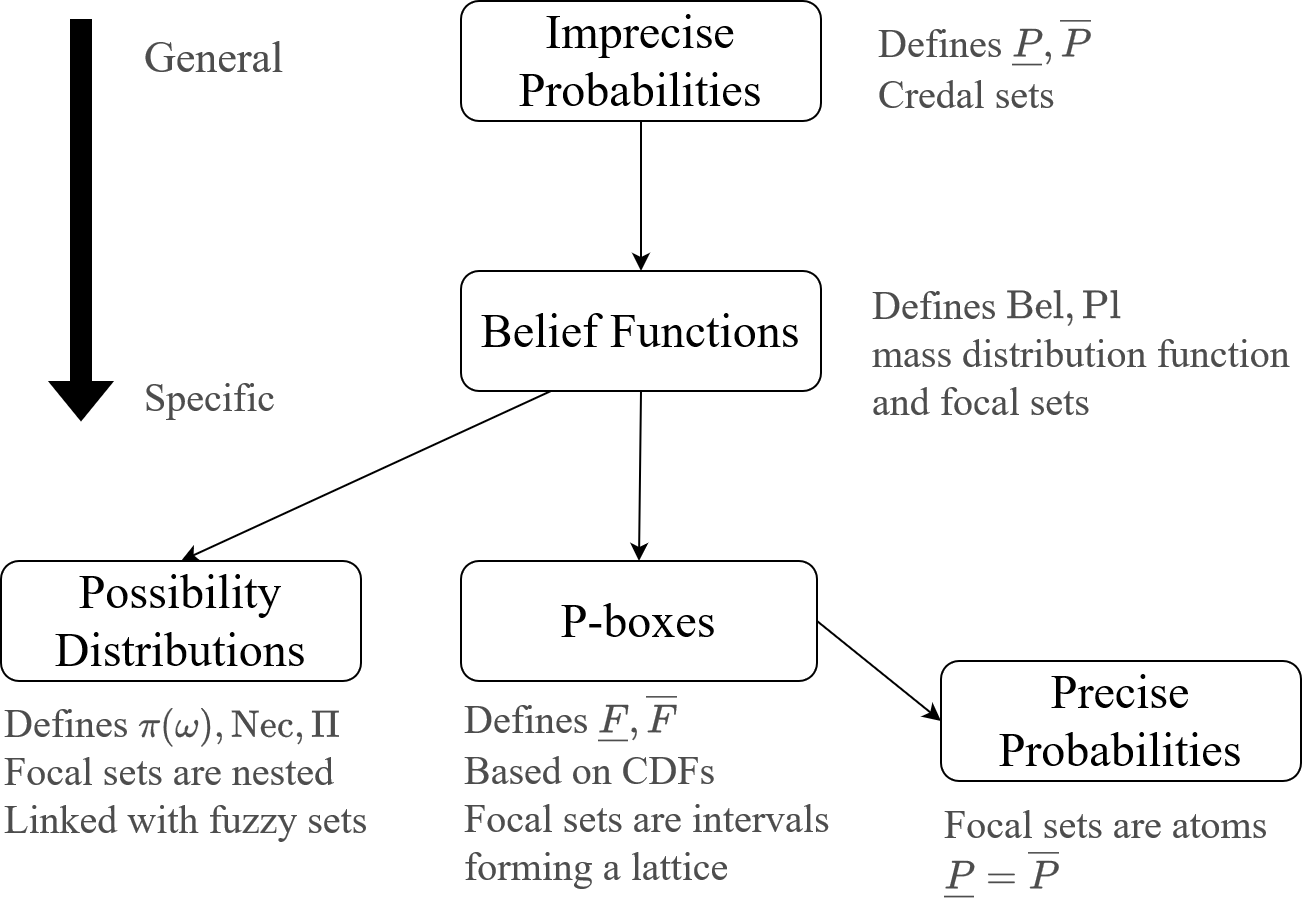
\includegraphics[width=0.8\linewidth]{Images/Chap_2/Diagramme_IP_Bel.png}
    \caption{Diagram representing the relationship between different Imprecise Probabilities models presented throughout \Cref{sec:different_models_of_uncertainty}.}
    \label{fig:diagram_IP}}
\end{figure}\commanue{La figure est bien pour voir les liens après je ne sais pas s'il faut garder les éléments en gris clair, c'est un peu déroutant pour le lecteur qui découvre les éléments}

As stated previously, a core concept of imprecise probabilities are lower and upper probabilities. Similarly to precise probabilities, a lower probability $\low$ and an upper probability $\overline{P}$ are mappings from a $\sigma$-algebra $\mathcal{A}$ to $[0, 1]$. However, while a probability $P$ gives a single measure of uncertainty for every event, lower and upper probabilities provide two bounds for every event, allowing them to express more complex uncertainty structures.

\begin{remark}
    Formally, a lower probability $\low$ needs to be \textit{super-additive}, \ie to verify:
    \begin{equation}
        \forall A,B\in\mathcal{A}, \text{ if } A\cap B\neq\emptyset, ~\low(A\cup B)\geqslant \low(A)+\low(B) \label{eq:super_additivity}
    \end{equation}
    Conversely, an upper probability is sub-additive, meaning that it verifies the same property than \cref{eq:super_additivity} but with the inequality reversed.
    
    Those properties are less constraining than their equivalent for precise probabilities in definition \ref{def:probability_space}, so lower and upper probabilities are generally \textit{not} precise probabilities. The only case where they are precise probabilities is when $\low=\overline{P}$, because $\low$ is then additive as it is both super and sub-additive. In this case, imprecise probabilities are actually a single precise probability. This illustrates the fact that precise probabilities are special cases of imprecise probabilities. 
\end{remark}

Precise probabilities define a measure of uncertainty towards a random variable $X$ taking numerical values. Imprecise probabilities however, can model the uncertainty towards a random variable taking set values instead of numerical one. We then say that $X$ is a \textit{random set} instead of a random variable. That being said, IP can also represent the uncertainty of random variables for which we suppose a precise probability exists, but we are not able to determine it precisely. Indeed, lower and upper probabilities form the bounds of a family of precise probabilities called \textit{credal set}.
\begin{definition}[Credal set]\label{def:credal_set}
    Given a lower probability $\low$ and an upper probability $\overline{P}$, a credal set $\M$ is the set of all probabilities $P$ that are greater that $\low$ and lower that $\overline{P}$:
    \begin{equation}
        \M(\low, \overline{P}) = \{P~|~\forall A\in\mathcal{A},~\low(A)~\leqslant~P(A)~\leqslant\overline{P}(A)\}
    \end{equation}
\end{definition}
We refer to $\M(\low, \overline{P})$ as $\M$ when no confusion is possible. Credal sets allow to consider multiple probabilities at once, which improves on the limited expressiveness of a single probability measure. The gap between the two bounds of a credal set reflects how imprecise is the model, in terms of epistemic uncertainty.

Conversely, we can define lower and upper bounds from a set of probabilities $\M$ as:
\begin{align*}
    \forall A\in\mathcal{A},~\low(A) =& \inf_{P\in\M}P(A)\\
    \forall A\in\mathcal{A},~\overline{P}(A) =& \sup_{P\in\M}P(A)
\end{align*}

Although, it is not required, we usually assume credal sets verify additional properties expressed as follows:
\begin{definition}[Coherence and Avoiding sure loss]\label{def:coherence_sure_loss}
    A credal set $\M$ is said to avoid sure loss if it contains at least one probability measure, \ie if
    \begin{equation}
        \M \neq \emptyset\label{eq:avoid_sure_loss}
    \end{equation}
    
    A credal set $\M$ is said to be \textit{coherent} if its lower and upper bounds on all events are attained by a probability measure, \ie if:
    \begin{equation}
        \forall A\in\mathcal{A}, \exists P, P'\in\M~\st~\low(A)=P(A) \text{ and } \overline{P}(A)=P'(A) 
    \end{equation}
\end{definition}
The bounds $\low, \overline{P}$ of a coherent credal set verifies the following property:
\begin{equation}
    \forall A\in\mathcal{A}, ~\low(A) = 1 - \overline{P}(A^c)\label{eq:lower_proba_complement}
\end{equation}
which is a generalization of the classical property for computing the complement of an event with precise probabilities. This allows us to only specify the lower bound $\low$ of a credal set to completely describe it, as its upper bound is determined by $\low$. Defining a credal set requires to specify much more constraints on the probability space that in the case of probability distributions. Indeed a lower probability must be defined on every possible event, while a precise probability can be defined by its density on possible values only (instead of possible events). In the case of a discrete space with $n$ elements, a probability is completely determined by its values on the $n$ atoms, while a lower bound is completely determined by its values on the $2^n$ considered events.


\begin{remark}
    Sampling from a credal set is not straightforward. Multiple method exists, the most intuitive consisting in sampling distributions from the credal set extreme points.
\end{remark}

\begin{remark}
    With the way we defined a credal set $\M$, it is closed and convex. This is a common way of constructing credal sets, but is not the only way. We could for instance impose that all probabilities in $\M$ belong to a family of Gaussian probabilities, which would prevent $\M$ from being convex.
\end{remark}

When constructing credal sets, it is common to possess a non convex set of probabilities $S$. In that case, we can define the convex hull of a set of probabilities $S$:
\begin{definition}[Convex Hull]\label{def:convex_hull}
    The convex hull ($CH$) of a set of probabilities $S$ is the smallest (convex) credal set containing $S$:
    \begin{equation}
        CH(S) = \{~P~|~\forall A\in\mathcal{A}, ~\inf_{P_S\in S}P_S(A)\leqslant P(A) \leqslant \sup_{P_S\in S}P_S(A)\}
    \end{equation}
\end{definition}

\begin{remark}
    The convex hull is computationally heavy to compute \commanu{redondant, juste is not computer-efficent, en tout cas pas 2 fois compute ;)}. Determining the infimum and supremum of a set of probability is not trivial as it might require to iterate through every element of $S$. It is however very useful, especially in the case where we do not know the set bounds on every event. In that case, computing the convex hull also allows us to determine the bounds on those events.
\end{remark}

\begin{example}
    Let us consider the scenario presented in example \ref{ex:proba_limitations}, and model the uncertainty with a credal set instead of a single probability distribution. Because we have no information on the value written on the card except that it is in $\{1,2,3\}$, we characterize the uncertainty by lower and upper probability $\low$, $\overline{P}$ defined as follows:
    \begin{align*}
        &\low(X=1) = \low(X=2)= \low(X=3) = 0\\
        &\overline{P}(X=1) = \overline{P}(X=2)= \overline{P}(X=3) = 1\\
        &\low(X\in\{1,2,3\}) = \overline{P}(X\in\{1,2,3\}) = 1
    \end{align*}
    We can use \cref{eq:lower_proba_complement} for computing the bounds of remaining events.
    
    Here, the credal set is the largest credal set possible as its bounds are always $0$ and $1$ for events that are not $\emptyset$ or $\{1,2,3\}$. We say that it is the vacuous credal set, as it does not encode any information. It however solves the problem of a contradicting probability when evaluating the value of the card and its parity.\commanue{J'aime bien le fait de présneter l'exemple. Après j'ai des difficultés à comprendre les deux dernières phrases.}\comloic{juste pour être sur de comprendre la dernière phrase, est ce que ça veut dire que dans le premier cas on avait une contradiction car on aurait pu vouloir d'abord fixer P(Y=pair) et P(Y=impair) et se retrouver avec P(X=1)=P(X=3)=1/4, alors que là si on commence à fixer Plower et Pupper sur X ou a Pupper(Y=impair)<=2 et Plower(Y=impair)>=0 ce qui n'est pas contradictoire avec Pupper(Y=impair)=1 et Plower(Y=impair)=0 que l'on aurait fixer dans ce mode opératoire là si on n'avait pas au préalable fixer les Pupper et Plower sur X ? }
\end{example}

\subsection{Belief Functions}\label{sec:belief_functions}
A special case of imprecise probabilities are belief functions, which we will detail in this section. First, we will introduce a key concept that goes along belief functions: mass distribution functions. We will then derive belief functions from it.

\begin{definition}[Mass distribution function]\label{def:mass_distribution_function}
    Let $\X$ be a frame of discernment\commanue{alrs X à la base c'est set of possible outcomes et là tu donnes un autre nom c'est pour la même chose ou il y a une subtilité. J'aime pas les variables qui changent surtout quand je suis pas à l'aise dans le domaine}\comloic{ah ouais +1 là t'es dur avec nous}\commanu{en effet ;)} and $2^\X$ its power set. A mass distribution function (or basic probability assignment \cite{shafer_mathematical_1976}) is a function $m:2^\X\rightarrow[0,1]$ \st:
    \begin{align}
        m(\emptyset) =& 0\label{eq:mass_emptyset}\\
        \sum_{a\subseteq\X}m(a) =& 1\label{eq:mass_whole_set}
    \end{align}
\end{definition}

There are multiple ways of interpreting $m(a)$, presented bellow\commanu{below, mais la tournure de la phrase me parait lourde:}, so as to be more familiar with $m$\commanu{pas évident de comprendre ce que tu expliques: la fonction de distribution de masse ou un sous ensemble ? est ce que cette phrase peut etre tournée sans m(a) et m et avec leur description en anglais?}:
\begin{itemize}
    \item If we consider a random set $X$, then $m(a)$ encodes the probability mass that $X$ takes $a$ as its set value.
    \item If $X$ is a random variable, then $m(a)$ encodes the available evidence that the numerical value of $X$ is \textit{exactly} in $a$, without any preferences for the values within $a$. This mean there could also be another evidence that $X$ is in $a'\subset a$, encoded with $m(a')$, and which could be either lower or higher than $m(a)$ depending on the amount of evidence available. Example \ref{ex:bicycle_pressure} illustrates this with a toy scenario. 
    \item Another interpretation of $m(a)$ is to link it to probability masses (definition \ref{def:density})\commanue{C'est bizarre de dire anaother car le premier parle déjà du lien entre m(a) et probability mass. Peut-être dire precise probability mass pour que ce soit plus clair}. If we suppose there exists an unknown underlying probability measure $P$ for $X$, $m(a)$ measures the probability mass that is assigned to $a$, but that can move freely to every point of $a$ without any preference. In other words, with more information, we could distribute $m(a)$ to every elements of $a$, and doing this for all $a$ would lead to a precise probability mass distribution.
\end{itemize}

\begin{remark}
    \Cref{eq:mass_emptyset} translates the fact than there is no evidence that the uncertain variable belongs to the empty set, \ie that it is not defined. Releasing this constraint allows to accept a certain amount of contradiction in our model.
    \Cref{eq:mass_whole_set} is a convention, which states that the total amount of evidence equals $1$. It is similar to probabilities which cannot be more than $1$. 
\end{remark}

\begin{definition}[Focal set]\label{def:focal_set}
    Let $\X$ be a frame of discernment\commanue{Même remarque que précédemment sur X}, $2^\X$ its power set, and $m:2^\X\rightarrow[0,1]$ a mass distribution function. A set $a\subseteq\X$ is called a focal set of $m$ if and only if:
    \begin{align}
        m(a)>0\label{eq:focal_set}
    \end{align}
\end{definition}
Focal sets thus represent sets of the frame of discernment for which we have evidence. The set of all focal sets is sometimes called the \textit{core} of $m$.

\begin{definition}[Belief function, Plausibility function]\label{def:belief_plausibility}
    Let $\X$ be a frame of discernment, $2^\X$ its power set, and $m:2^\X\rightarrow[0,1]$ a mass distribution function.
    
    We define the belief function associated with $m$ as the function $\Bel:2^\X\rightarrow[0,1]$ who associates to all events $A$ in $2^\X$:
    \begin{align*}
        \Bel(A)=\sum_{a\subseteq A} m(a)
    \end{align*}
    
    We define the plausibility function associated with $m$ as the function $\Pl :2^\X\rightarrow[0,1]$ who associates to all events $A$ in $2^\X$:
    \begin{align*}
        \Pl(A)=\sum_{\substack{a\\a\cap A\neq\emptyset}} m(a)
    \end{align*}
\end{definition}
We can interpret $\Bel(A)$ as the amount of evidence that fully support $A$, and $\Pl(A)$ as the amount of evidence that is consistent (or does not contradict) with $A$.

$\Bel$ and $\Pl$ are special cases of lower and upper probabilities, and verify \eqref{eq:lower_proba_complement} as for all events $A$ it holds:
\begin{align*}
    \Bel(A)&=\sum_{a\subseteq A} m(a)\\
    &= \sum_{a\in \X} m(a) - \sum_{a\not\subseteq A} m(a)\\
    &= 1 - \sum_{\substack{a\\a\cap A^c\neq\emptyset}} m(a)\\
    &=1-\Pl(A^c)
\end{align*}

Belief functions possess interesting properties making the credal set they induce both coherent and avoiding sure loss, motivating their extensive usage.

\begin{example}[Defining mass and belief\commanue{manque plausibility} functions]\label{ex:bicycle_pressure}
    Let us imagine an experiment where you try to estimate the pressure of the tyres of your bike, but your bicycle pump only have graduation every $1$ bar. You are able to do three measurements:
    \begin{itemize}
        \item The first measure, the needle seems to be between $4$ and $5$ bar.
        \item The second measure, the needle seems to be between $4.5$ and $6$ bar.
        \item The third measure, the needle seems to be between $4.5$ and $5.5$ bar.
    \end{itemize}
    Let us say that you trust your last measurement the most, because you got used to the movement of the needle. It is now possible to model the uncertainty of your tyre pressure using available evidence encoded in $m$:\\
    \noindent
    \begin{minipage}{0.3\textwidth}
        \begin{align*}
            m([4,~5]) ~=~ 0.3
        \end{align*}
    \end{minipage}\hfill
    \begin{minipage}{0.3\textwidth}
        \begin{align*}
            m([4.5,~6]) ~=~ 0.3
        \end{align*}
    \end{minipage}\hfill
    \begin{minipage}{0.3\textwidth}
        \begin{align*}
             m([4.5,5.5]) ~=~ 0.4
        \end{align*}
    \end{minipage}\par
    Based on this, we are no\comloic{je suppose que c'est now mais le chapitre 2 me consomme pas mal de matière grise et ce matin j'ai pas un gros stock disponible} able to express our degree of belief and of plausibility for all events. For instance:
    \begin{itemize}
        \item Our degree of belief that the pressure lies in $[4, 5]$ is $\Bel([4, 5])=0.3$, that it lies in $[4, 5.5]$ is $\Bel([4, 5.5])=0.7$ and that it lies in $[4, 6]$ is $\Bel([4, 6])=1$
        \item The degree of plausibility that the pressure equals $5$ is $\Pl (5)=1$ (totally plausible), that it equals $5.5$ is $\Pl (5.5)=0.7$ and that it equals $4$ is $\Pl (4)=0.3$.
    \end{itemize}
\end{example}

\subsection{Possibility Distributions}\label{sec:possibilities}
Another convenient model of uncertainty are possibility distributions\comloic{je me suis un peu perdu dans la structure ici. J'avais noté trois façon de modéliser l'incertitude épistémique dans le 2.3.0. Dont les proba imprécises que l'on a présenté 2.3.2. Ici l'intro c'est qu'on présente un autre modèle. Est ce qu'il manque un tiret dans le 2.3.0 ? Est ce que c'est un sous modèle des proba imprécises ? Je me mélange un peu tout seul peut être. Ah j'ai retrouvé ma réponse dans le 2.3.0: 2.3.4 et 2.3.5 sont des cas spécifiques de 2.3.2. Et bein est ce qu'on peut pas indicer les titres avec un niveau inférieur pour montrer qu'on n'est pas au meme niveau que 2.3.1 (proba précises) et 2.3.2 (imprécises) mais qu'on est dans les proba imprécises ?}. We will see that they induce a particular type of belief functions, and will be used in our applications.

\begin{definition}[Possibility distribution]\label{def:possibility}
    Let $\X$ be the frame of discernment. A possibility distribution is a function $\pi: \X \rightarrow [0,1]$ satisfying:
    \begin{equation}
    	\exists x \in \X, \pi(x) = 1 \label{eq:possibility}
    \end{equation}
    The value $\pi(x)$ represents the degree of possibility of $x$, with $\pi(x) = 1$ indicating full possibility, and $\pi(x) = 0$ indicating impossibility.
\end{definition}

Another notion closely related to possibility distributions is that of \(\alpha\)-cuts:
\begin{definition}[\(\alpha\)-cut]\label{def:alpha_cut}
    Let $\pi: \X \rightarrow [0,1]$ be a possibility distribution. Given any \(\alpha\in[0,1]\), we define the \(\alpha\)-cut of \(\pi\) as:
    \begin{align}
        \alpha_\pi=\{x~|~\pi(x)\geqslant\alpha\} \label{eq:alpha_cut}   
    \end{align}
    An \(\alpha\)-cut is thus the set of all elements of $\X$ whose possibility level is more that $\alpha$.
\end{definition}

\begin{definition}[Necessity and Possibility measures]
    It has been proven in \cite{dubois_when_1992} that a possibility distribution defines a specific type of plausibility functions called \textit{possibility} function and noted \(\Pi\). It also defines a specific belief function by duality called \textit{necessity} function and noted \(\Nec\), as well as a credal set $\M(\pi)$. They are defined as:
    \begin{align}
        &\Pi(A) = \sup_{x\in A}\pi(x)\\
        &\Nec(A)=1-\sup_{x\in A^c}\pi(x)\label{eq:bel_pl}\\
        &\M(\pi) &=\{P~|~\forall A,~P(A)\leqslant \sup_{x\in A}\pi(x)\}\\
        &=\{P~|~\forall A,~P(A)\leqslant \Pi(A)\} \label{eq:credal_set_possibility}\\
        &= \{P~|~\forall A,~P(A)\geqslant \Nec(A)\}
    \end{align}
\end{definition}

\begin{example}[Defining a possibility distribution]\label{ex:bicycle_pressure_possibility}
    Let us imagine the same setting as example \ref{ex:bicycle_pressure}, where we try to estimate the pressure of the tyres of our bike, but our bicycle pump only have graduation every $1$ bar. We are able to do the following measurements:
    \begin{itemize}
        \item During the first measurement, the needle seems to be around $4$ bar.
        \item During the second measurement, the needle seems to be around $5$ bar.
        \item During the third measurement, the needle seems to be around $4.5$ bar.
    \end{itemize}
    Let us say that we trust our measurement with a precision of plus or minus $0.5$ bars. For simplicity, we also only consider pressure values that are integers or half integers. Taking into considerations all the measurements, we can define a possibility distribution $\pi$ as:
    \begin{itemize}
        \item The value of $4.5$ being the most possible, $\pi(4.5)=1$.
        \item Values between $4$ and $5$ bar being mostly possible, we can for instance fix $\pi(4)=\pi(5)=0.8$
        \item Values $3.5$ and $5.5$ are unlikely but not impossible, we can say that $\pi(3.5)=\pi(5.5)=0.3$
        \item Other values are impossible, and thus have a possibility of $0$.
    \end{itemize}
    The possibility distribution $\pi$ is represented in \Cref{fig:possibility_distribution}
    Based on this, we are no\comloic{now aussi j'imagine} able to express the degree of necessity and of\commanu{j'enleverais le 2ieme of} possibility for all events. For instance:
    \begin{itemize}
        \item The degree of necessity that the pressure lies between $4$ and $5$ bar is $\Nec([4, 5])=1-\sup_{\rho\not\in[4,5]}\pi(\rho)=0.7$
        \item The degree of necessity that the pressure lies between $3.5$ and $5.5$ bar is $\Nec([3.5,~ 5.5]) = 1-\sup_{\rho\not\in[3.5,5.5]}\pi(\rho) = 1$\comroman{Retour à la ligne avant l'équation?}, meaning that the pressure is necessarily in this range.
        \item The degree of possibility that the pressure is either $3.5$ or  $5$ is $\Pi (\{3.5,~5\})=\sup_{\rho\in\{3.5,~5\}}\pi(\rho)=0.9$ (mostly possible).
        \item \etc for every possible event.
    \end{itemize}
\end{example}

\begin{figure}[!ht]
    \centering
    \begin{tikzpicture}[scale=1]
        \begin{axis}[%
          xlabel=Pressure $\rho$ (in bar),
          ylabel=$\pi(\rho)$,
          xmin=2, xmax=7,
          ymin=-0.1, ymax=1.1,
          ytick={0, 0.3, 0.8, 1},
          yticklabels={$0$, $\alpha=0.3$, 0.8, $1$},
          ],
          \node (a) at (2, 0) {$\times$};
          \node (b) at (2.5, 0) {$\times$};
          \node (c) at (3, 0) {$\times$};
          \node (d) at (3.5, 0.3) {$\times$};
          \node (e) at (4, 0.8) {$\times$};
          \node (f) at (4.5, 1) {$\times$};
          \node (g) at (5, 0.8) {$\times$};
          \node (h) at (5.5, 0.3) {$\times$};
          \node (i) at (6, 0) {$\times$};
          \node (j) at (6.5, 0) {$\times$};
          \node (k) at (7, 0) {$\times$};
          
          \draw [thick, dashed, gray] (a.center) -- (b.center) -- (c.center) -- (d.center) -- (e.center) -- (f.center) -- (g.center) -- (h.center) -- (i.center) -- (j.center) -- (k.center) ;
          \draw [<->, >=latex, ultra thick, blue] (d.east) -- (h.west) node [pos=0.5, above] {$\alpha_\pi$};
        \end{axis}
    \end{tikzpicture}
    \caption{Possibility distribution of example \ref{ex:bicycle_pressure_possibility} and one of its $\alpha$-cut in blue}
    \label{fig:possibility_distribution}
\end{figure}

\begin{remark}
    If you are familiar with fuzzy sets you may have noticed than\comloic{that?} possibility distributions strongly resemble\commanu{is very similar ?} to the membership function of a fuzzy set. Links between fuzzy sets and possibility measures have been explored in \cite{zadeh_fuzzy_1999}.
\end{remark}

Focal sets of necessity functions can be determined directly from the possibility distribution by looking at their \( \alpha \)-cuts. It has been proven that the core $\mathcal{C}$ (the set containing all focal sets) of a necessity function is (\cite{destercke_unifying_2008}):
\begin{align*}
    \mathcal{C} =& \{\alpha_\pi~|~\alpha\in[0,1]\}\\
    =& \{ ~\{x\in\X~|~\pi(x)\geqslant\alpha\}~|~\alpha\in[0,1]~\}
\end{align*}
With the way focal sets are defined, they form a nested family of sets with regards to inclusion. Indeed, if an element of \(\X\) belongs to an \(\alpha\)-cut, then its possibility is greater than \(\alpha\) and therefore belongs to any other \(\alpha'\)-cut with a lower \(\alpha'\). For simplicity, we will suppose that the focal sets \(a_1\enum a_n\) are already numbered using the inclusion order, \ie \( a_1\subset\dots\subset a_n\). In this case, we will refer to the inclusion order as the ``natural'' order.

\begin{remark}
    The fact that focal sets form a nested family of sets in the case of possibility distributions also implies than if $\X$ is finite and contains $n$ elements, then there can be \textit{at most} $n$ focal sets. For comparison, belief functions can have a maximum of $2^n-1$ focal sets (as the empty set cannot be a focal set). This means that necessity functions have less degrees of freedom than (some) belief functions and thus can express less uncertainty structures. This drawback comes with the advantage of being easier to construct, as we only need to specify the mass of $n$ focal sets (or the possibility of the $n$ elements of $\X$) instead of $2^n-1$. Indeed, when we think of a random variable like the outcome of a dice, it can seem more natural for someone to specify degrees of possibility for each side separately than it is to specify degrees of plausibility for different sets of outcomes. 
    
    As such, possibility distribution have been used to model experts opinion  \cite{baudrit_joint_2007}. Following the same philosophy, we will use possibility distributions in \Cref{chap:epistemic_uncertainty} to model the uncertainty of a measure of similarity between two image patches.
\end{remark}

Specifying a probability distribution often comes down to specifying the probability mass function over all atoms of the frame of discernment. In a way, possibility distributions are constructed the same way, as we specify the possibility (or the upper bounds) of every atom. One important difference is that the condition ``the sum of all masses must be equal to $1$'' is relaxed into a less constraining condition ``the possibility distribution must be equal to $1$ at least once''. In that respect, it is easier to construct a well defined possibility distribution than it is to construct a well defined probability distribution. However the comparison stops there, as the two models does not represent the same uncertainty at all.

\begin{remark}
    Any probability distribution $P$ is a belief function $\Bel$, for which focal sets are only composed of singletons (atoms) and the mass distribution function of $\Bel$ equals the probability mass function of $P$ on atoms. However, a possibility distribution cannot model a probability distribution. Indeed this would impose that its necessity $\Nec$ and plausibility $\Pi$ functions verify:
    \begin{align*}
        \forall A, &~\Nec(A) = \Pi(A)\\
        \Leftrightarrow&~1-\sup_{x\in A^c}\pi(x) = \sup_{x\in A}\pi(x)\\
        \Leftrightarrow&~ \sup_{x\in A}\pi(x) + \sup_{x\in A^c}\pi(x) = 1
    \end{align*}
    Consider this equation for any $x'$ verifying $\pi(x')=1$. This leads to the conclusion that any $x\neq x'$ has a possibility of $0$. We are in a case where it is impossible that a random set or random variable takes any other value than $x'$, which makes it not random. 
\end{remark}

\subsection{P-boxes}\label{sec:pboxes}
Another special type of belief function that is commonly used is that of \textit{probability boxes}, more commonly called p-boxes. Formally, a p-box is a pair of precise cumulative distribution functions $[\underline{F}, ~\overline{F}]$ defining lower and upper bounds on all cumulative events:

\begin{definition}[P-box]\label{def:p-box}
    Let $\X$ be the frame of discernment. A p-box is a pair of CDF $[\underline{F}, ~\overline{F}]$ from $\X$ to $[0, ~1]$ such that:
    \begin{equation}
    	\forall x \in \X,~\underline{F}(x) \leqslant \overline{F}(x) \label{eq:p-box}
    \end{equation}
    If $\X$ is not a subset of $\mathbb{R}$, then there must exists a total order on $\X$ to define a p-box. 
\end{definition}

\begin{remark}
    A probability distribution can be both determined by specifying its values on every atom or by specifying its values on cumulative events. We saw in \Cref{sec:possibilities} that possibility distributions define bounds on atoms. Because p-boxes define bounds on cumulative events, we could say that a p-box is the ``imprecise way'' of defining a probability using cumulative events, and a possibility distribution is the ``imprecise way'' of defining a probability using atoms.
\end{remark}

The credal set $\M$ induced by a p-box $[\underline{F}, ~\overline{F}]$ is:
\begin{align}
    \M([\underline{F}, ~\overline{F}]) = \{~ F ~|~ \forall x\in\X, ~\underline{F}(x)\leqslant F(x)\leqslant \overline{F}(x) ~\}
\end{align}

\begin{definition}[Focal sets of p-boxes]
    P-boxes are special cases of belief functions. It has been proven in \cite{destercke_unifying_2008} that focal sets of p-boxes have a specific form. Although focal sets shapes are reminiscent of possibilities' $\alpha$-cuts (see \Cref{fig:p-box}), they are a bit more complex to express formally. If $\X=\{x_1\enum x_n\}$ with $x_1\leqslant\dots\leqslant x_n$, then focal sets $\alpha_{[\underline{F}, ~\overline{F}]}$ of $[\underline{F}, ~\overline{F}]$ are given for every $\alpha\in[0,~1]$ by the following expression:
    \begin{align}
        \alpha_{[\underline{F}, ~\overline{F}]}= \opi \overline{F}^{-1}(\alpha),~\underline{F}^{-1}(\alpha)\cli\label{eq:pbox_focal_set}
    \end{align}
    where $\opi\cdot,~\cdot\cli$ are intervals of integers, and $\overline{F}^{-1}$, $\underline{F}^{-1}$ are the respective pseudo-inverse of $\overline{F}$ and $\underline{F}$ defined for every $\alpha\in[0,1]$ by:
    \begin{align*}
        \overline{F}^{-1}(\alpha) =& \min \{x_i ~\st ~\overline{F}(x_i)\geqslant \alpha\}\\
        \underline{F}^{-1}(\alpha) =& \min \{x_i ~\st ~\underline{F}(x_i)\geqslant \alpha\}\commanue{c'est pas un max?}\comloic{alors de ce que je comprends grace à la figure 2.3 (parce que bon avec le texte j'y étais pas non plus), c'est un max seulement si on cherche xi tel que Funder <= xi. Du coup ça a l'air ok.}
    \end{align*}
    
    Still in \cite{destercke_unifying_2008}), it has been shown that the mass of each focal set $\opi x_i, ~x_j\cli$ equals to :
    \begin{align}
        m(\opi x_i, ~x_j\cli) = \min(\overline{F}(x_i), \underline{F}(x_j)) - \max(\overline{F}(x_{i-1}), \underline{F}(x_{j-1}))
    \end{align}
    With the convention that $\max(\overline{F}(x_{i-1}), \underline{F}(x_{j-1}))=0$ if $x_{i}$ is the first element and thus $x_{i-1}$ is ill-defined. 
\end{definition}

Because of their shape, focal sets of p-boxes form a lattice on $\X$, and can be ordered. It can be easily seen by looking at \Cref{fig:p-box}. If $a$ and $b$ are two focal sets of the same p-box $[\underline{F}, ~\overline{F}]$, then they are ordered as follows:
\begin{align}
    a\leqslant b \Leftrightarrow \min(a)\leqslant\min(b) \text{ and } \max(a)\leqslant \max(b)
\end{align}
As $\underline{F}\leqslant\overline{F}$, we are assured that there can't be any case where $\min(a)<\min(b) \text{ and } \max(a)> \max(b)$\commanue{Tu t'es pas trompé de signe pour le min ?}. We can also define the order on focal sets using the definition of \cref{eq:pbox_focal_set} for every $\alpha,~\beta\in[0,1]^2$:
\begin{align*}
    \opi\overline{F}^{-1}(\alpha), ~\underline{F}^{-1}(\alpha)\cli \leqslant \opi\overline{F}^{-1}(\beta), ~\underline{F}^{-1}(\beta)\cli \Leftrightarrow \alpha\leqslant\beta
\end{align*}

Given the shape of focal sets, there can be at most $2n-1$ in a frame of discernment with $n$ elements\comloic{ça c'est un truc que j'ai encore du mal à dessiner}. This is more degree of freedom than possibility distributions, but less than general belief functions.
\begin{remark}
    Contrary to possibility distributions that cannot equal to a single probability distribution, if a p-box $[\underline{F}, ~\overline{F}]$ verifies $\underline{F}=\overline{F}$, then its credal set is composed of a single probability distribution whose CDF $F$ equals $\underline{F}$ and $\overline{F}$. P-boxes are thus generalizations of precise probability distributions.
    
    Because both $\underline{F}$ and $\overline{F}$ are precise CDF and belong to the credal set $\M([\underline{F}, ~\overline{F}])$, we already know two samples of the credal sets it defines, without having to sample from it.
\end{remark}

\begin{figure}[!ht]
    \centering
    \begin{tikzpicture}[scale=1]
        \begin{axis}[%
          xlabel=$x$,
          ylabel=$\CDF(x)$,
          %grid=major,
          domain=0:15,
          %legend entries={$\underline{F}$, $\overline{F}$},
          legend pos=south east,%
          ],
            \addplot[dotted, black, samples=16, mark=triangle, mark options={solid}, mark size=3pt] {cdf_erf(x, 1.5, 1.5)} node [pos=0.4, above left] {$\overline{F}$};
            \addlegendentry{$\overline{F}$}
            
            \addplot[dotted, black, samples=16, mark=square, mark options={solid}, mark size=3pt] {cdf_erf(x, 7.5, 1.5)} node [pos=0.6, below right] {$\underline{F}$};
            \addlegendentry{$\underline{F}$}
            
            \addplot[dotted, gray, samples=16, mark=+, mark options={solid, color=gray}, mark size=3pt] {cdf_erf(x, 4.5, 2)};
            \addlegendentry{$F$}
            
            \node (a) at (4, {cdf_erf(4, 1.5, 1.5)}) {};
            \node (b) at (10, {cdf_erf(10, 7.5, 1.5)}) {};
            
            \draw [<->, >=latex, ultra thick, blue] (a.east) -- (b.west) node [pos=0.5, above] {$\alpha_{[\underline{F}, ~\overline{F}]}$};
        \end{axis}
        \end{tikzpicture}
    \caption{A p-box $[\underline{F}, ~\overline{F}]$, a precise CDF $F$ in its credal set, and one of its focal elements $\alpha_{[\underline{F}, ~\overline{F}]}$ in blue}
    \label{fig:p-box}
\end{figure}


\section{Dependency Models: Copulas}\label{sec:copulas}
During previous sections, we presented different models of uncertainty that will be considered throughout this thesis. When we will aggregate and propagate multiple sources of uncertainty in chapters \ref{chap:joining_credal_sets}, \ref{chap:propagating} and \ref{chap:epistemic_uncertainty}, we will need to take into account the dependency between our uncertain sources. In this section, we will present dependency models called copulas, which are mathematical tools used to represent the dependency between multiple random variables. Copulas can represent many types of dependency, ranging from complete monotonicity to complete counter-monotonicity, including independence between variables. \Cref{sec:copula_def} will present the mathematical definition of a copula as well as practical families of copulas and how they can model different dependencies. \Cref{sec:dconvexity} will present a specific property shared by some copulas and a theoretical contribution that will \commanu{be ?}used later in sections \ref{subsec:pboxes} and \ref{subsec:multiple_models}. Finally, we present how to generate multivariate samples from a copula, which will be used in \Cref{sec:montecarlo}.

\subsection{Core Definitions and Examples}\label{sec:copula_def}
In the following, let $n\in\mathbb{N}^*$ be the number of sources of uncertainty considered (either represented by random variables or random sets). We first introduce copulas, which are mapping from $[0,1]^n\rightarrow [0,1]$ verifying a number of properties, and that can model dependencies when considering \hyperref[theorem:sklar]{Sklar's Theorem}, which will be presented in this section.

\begin{definition}
     A copula is a multivariate cumulative distribution function $C:[0,1]^{n}\rightarrow [0,1]$ whose marginals follow uniform distributions on $[0,1]$. It can be interpreted as a joint cumulative distribution of $n$ random variables. For all $i\in\opi 1,n\cli $, we will refer to $u_i\in[0,1]$ as its $i$-th variable (or marginal). A copula verifies a number of properties:
\begin{align}
    &\text{if }\exists j\in\opi 1,n\cli  \text{ \st }~u_j=0, \text{ then }C(u_1\enum u_j\enum u_n)=0\label{eq:zero_copula}\\
    &\forall i\in\opi 1,n\cli ,~C(1,1\enum1,u_i,1\enum1)=u_i\label{eq:copula_ones}\\
    &\forall (v_1\enum v_n)\in[0,1]^n \text{ \st }~\forall i\in\opi 1,n\cli ,~v_i\geqslant u_i\nonumber\\
    &\sum_{(w_1\enum w_n)\in\Pi_{i=1}^n\{u_i, v_i\}}(-1)^{|\{i~|~w_i=u_i\}|}C(w_1\enum w_n)\geqslant 0\label{eq:cop_hvolume}
\end{align}
where $\Pi_{i=1}^n$ is the Cartesian product of $n$ elements, meaning that $(w_1\enum w_n)\in\Pi_{i=1}^n\{u_i, v_i\}$ is a tuple of $n$ elements, where each element is either $u_i$ or $v_i$. Additionally, $|\{i~|~w_i=u_i\}|$ refers to the cardinal of the set $\{i~|~w_i=u_i\}$. 
\end{definition}

The first term in \cref{eq:cop_hvolume} is also called H-volume or hyper-volume. It is used to compute joint probability mass assignments in the precise case (and also in the imprecise case, see \Cref{sec:joint_mass}). In the rest of this thesis\commanu{j'aime pas trop in the rest, très french, We will now use... seulement?}, we will use the following notation to refer to the $H$-volume:
\begin{eqnarray}\label{eq:hvolume}
    &&\forall i\in\opi 1,n\cli ,~\forall~0\leqslant u_i \leqslant v_i \leqslant 1,\nonumber\\
    &&H^{v_1,\dots v_n}_{u_1\enum u_n}=\sum_{(w_1\enum w_n)\in\Pi_{i=1}^n\{u_i, v_i\}}(-1)^{|\{i~|~w_i=u_i\}|}C(w_1\enum w_n)
\end{eqnarray}

\begin{remark}
    The formula of the H-volume actually represents the probability that $n$-uniform random variables are in the hyper rectangle $[u_1,v_1]\tdt[u_n,v_n]$. However, it is difficult to see this interpretation in the general case just by looking at the formula. For simplicity, consider the two dimensional case. Using the interpretation of a copula $C$ as a CDF, we can image two random uniform variables $U_1$ and $U_2$ on $[0,1]$ for which $C$ is their CDF. We thus have for all $(u_1,u_2)\in[0,1]^2$:
    \begin{equation*}
        P(U_1\leqslant u_1, U_2\leqslant u_2) = C(u_1, u_2)
    \end{equation*}
    Let $(u_1,u_2)\in[0,1]^2$ and $(v_1,v_2)\in[0,1]^2$ \st $u_1\leqslant v_1$ and $u_2\leqslant v_2$. 
    Computing the H-volume of $C$ between $(v_1,v_2)$ and $(u_1,u_2)$, using different colors to help comprehension \commanu{understanding?}, yields:
    \begin{align}
        H^{v_1,v_2}_{u_1,u_2} =& ~C(v_1, v_2) - C(v_1, u_2) - C(u_1, v_2) + C(u_1, u_2)\nonumber\\
        =&~ \textcolor{blue}{P(U_1\leqslant v_1, ~U_2\leqslant v_2) - P(U_1\leqslant v_1, ~U_2\leqslant u_2)}\nonumber\\
        &- \textcolor{red}{P(U_1\leqslant u_1, ~U_2\leqslant v_2) + P(U_1\leqslant u_1, ~U_2\leqslant u_2)}\nonumber\\
        =&~ \textcolor{blue}{P(U_1\leqslant v_1, ~u_2 < U_2 \leqslant v_2)} - \textcolor{red}{P(U_1\leqslant u_1, ~u_2 < U_2\leqslant v_2)}\nonumber\\
        =&~ P(u_1 < U_1\leqslant v_1, ~u_2 < U_2\leqslant v_2)\label{eq:hvol_link_with_proba}
    \end{align}\comloic{alors là un grand merci parce que j'étais un peu coincé sur les notations dans l'eq (2.24), si j'avais su que tu avais préparé un exemple je m'y serais rendu direct ^^' En tout cas c'est bien plus clair comme ça, top!}
    This means that the H-volume represent the probability of the event
    \begin{equation*}
        u_1 < U_1\leqslant v_1, ~u_2 < U_2\leqslant v_2
    \end{equation*}
    or in other words, the probability that $(U_1, U_2)$ is in the hyper rectangle $[u_1,v_1]\times[u_2,v_2]$ (the intervals can be open or closed in the continuous case, the probability remains the same). Verifying this result can easily to the $n$-dimensional case can be done similarly\comloic{petit pb de formulation}. Example \ref{ex:hvolume} illustrates how the H-volume can be used to compute the discrete joint mass distribution function in the two-dimensional case. 
\end{remark}

A central theorem regarding copulas is \hyperref[theorem:sklar]{Sklar's Theorem} \cite{sklar_fonctions_1959}:
\begin{theorem}[Sklar's Theorem]\label{theorem:sklar}
    Let $F:\X_1\tdt\X_n\rightarrow[0,1]$ be a multivariate cumulative distribution function, where $\X_i\subseteq\overline{\mathbb{R}}$. The marginals $F_i$ of $F$ are defined as $\forall i\in\opi 1,n\cli , \forall x\in\X_i, F_i(x) = F( +\infty\enum  +\infty, x,  +\infty\enum +\infty)$ where $x$ is the $i$-th component of $F$. If all $F_i$ are continuous, then a unique copula $C$ exists:
    \begin{align}
        \forall (x_1\enum x_n)\in \overline{\mathbb{R}}^n, F(x_1\enum x_n)=C(F_1(x_1)\enum F_n(x_n))\label{eq:sklar_equality}
    \end{align}
    If some $F_i$ are not continuous, then $C$ is unique on the product of the ranges of all $F_i$.
    
    The reverse is also true: any copula applied to univariate cumulative distribution functions yields a multivariate cumulative distribution function whose marginals are the univariate CDFs.
\end{theorem}
\hyperref[theorem:sklar]{Sklar's Theorem} thus allow to express any multivariate CDF by means of its marginal CDFs. Conversely, we can join multiple CDF with a copula to create a multivariate CDF. A copula thus express the dependency between a multivariate CDF and its marginals.
 
\begin{remark}
    For marginals $F_i$ that are not continuous, then there can exist multiple copula $C$ verifying \cref{eq:sklar_equality}. However, if we note $F_i(\X_i)$ the image of $X_i$ through $F_i$, then there exists a unique copula $C$ on the ranges of images $F_1(\X_1)\tdt F_n(\X_n)$. The restriction of a copula \comloic{to?} a subset of $I^n$ containing $0$ and $1$ is called a sub-copula. Because we work in discrete spaces, we will mostly work with sub-copulas but the difference will be mostly transparent.
\end{remark}

Copulas are very useful to represent the dependency \comloic{je doute entre dependency et dependencies dans ce contexte} between multiple sources of uncertainty. As such, they can play a key role in uncertainty propagation problems, explored in \Cref{chap:propagating}.

\begin{example}[Usefulness of the H-Volume]\label{ex:hvolume}
    This example will illustrate how the H-volume of a copula can be used to compute the probability mass function of a multivariate probability. Let us imagine a game where a dealer throws two coins, and we are are interested in the joint result of the throws.\commanu{pas évident pour un néophyte de comprendre l'utilité du H-Volume dans ton exemple. Peut etre une phrase pour expliquer à quoi ca sert dans ton exemple du dealer, après tu pars vraiment dans l'explication technique math et on ne voit pas à quoi sert le H-Volume de façon imagée, à mon avis} We consider the two random variables $X_1$ and $X_2$ indicating the results of each throw:
    \begin{align*}
        &X_1=0\text{ if the first coin is heads, otherwise }X_1=1\\
        &X_2=0\text{ if the second coin is heads, otherwise }X_2=1
    \end{align*}
    Let $P_1$ and $P_2$ be the probability distributions of $X_1$ and $X_2$ respectively, and suppose that both heads and tails are possible outcomes for both coins. We now consider the joint probability distribution $P$ associated with the random variable $(X_1,~X_2)$, and we want to compute the probability mass distribution of $P$. We denote $F_1$, $F_2$ and $F$ the respective CDFs of $P_1$, $P_2$ and $P$. With this definition, $F_1$ and $F_2$ are the marginals of $F$, and Sklar's theorem states that there exists a copula $C$ such that $F=C(F_1,~F_2)$. 
    
    The probability mass distribution of $P$ can be computed by using the H-volume. Let us for instance start by computing $P(1,1)$. By noticing the fact that:
    \begin{equation*}
        \{x\in\X~|~X_1(x)=1\}=\{x\in\X~|~F_1(X_1(x))=F_1(1)\}
    \end{equation*}
    we can write that:
    \begin{align*}
        P(X_1 = 1, X_2=1) =& ~P(F_1(X_1)= 1, F_2(X_2) = 1)\\
        =& ~P(F_1(0) < F_1(X_1)\leqslant F_1(1), ~F_2(0) < F_2(X_2)\leqslant F_2(1))
    \end{align*}
    A common result in statistics states that random variables of the form $U_1=F_1(X_1)$ and $U_2=F_2(X_2)$ are uniform on $[0,1]$. We can thus apply the result from \cref{eq:hvol_link_with_proba}, which yields
    \begin{align*}
        P(X_1 = 1, X_2=1) =& ~P(F_1(0) < U_1 \leqslant F_1(1), ~F_2(0) < U_2 \leqslant F_2(1))\\
        =& ~H^{F_1(1),~F_2(1)}_{F_1(0),~F_2(0)}
    \end{align*}
    The probability of the atom $(1,1)$ is therefore equal to the H-volume computed between CDFs $(F_1, F_2)$ at $(1, 1)$ and at $(0,0)$. Following a similar reasoning, we can compute the probability of every atom and express them as H-volumes:
    \begin{align*}
        P(X_1=0, X_2=1) =& ~H_{0, F_2(0)}^{F_1(0), F_2(1)}\\
        P(X_1=1, X_2=0) =& ~H_{F_1(0), 0}^{F_1(1), F_2(0)}\\
        P(X_1=0, X_2=0) =& ~H_{0,0}^{F_1(0), F_2(0)}
    \end{align*}
    It is possible to generalize our observation: the probability of an atom $(x_1,~\dots,~x_n)$ is the H-volume computed between marginals CDFs $(F_1,~\dots,~F_n)$ at $(x_1,~\dots,~x_n)$ and at the marginal atoms that precedes them. If $x_1$ is the smallest number, then the marginal CDF $F_1$ before it equals $0$, \etc.
    Example \ref{ex:copulas} presents numerical applications of this example with different copulas.
\end{example}

It follows from \eqref{eq:cop_hvolume} that a copula is a component-wise increasing mapping. All copulas are actually dominating and dominated by two bounds (called lower and upper Fréchet–Hoeffding bounds):
\begin{align}
    &\forall u_i \in [0,1]^n,\nonumber\\
    &\max(0, 1-n+\sum_{i=1}^n u_i) \leqslant C(u_1\enum u_n) \leqslant \min(u_1\enum u_n)
\end{align}
The upper bound is a copula, usually called the Minimum copula $C_M$. It is used to model co-monotonic variables, \ie variables where high values occur at the same time (or similarly, where low values tend to occur simultaneously). Co-monotony implies a maximal covariance between variables.

The lower bound is a copula only in the case $n=2$, called the \L ukasiewicz copula $C_L$\commanue{Peut-être mettre la formule car tu mets celle pour plus de 2 dimensions}. It is used to model counter-monotonic variables, \ie variables with a perfect negative dependence between them. This explain why the lower bound is not a copula in dimensions higher that $2$ \commanue{Peut-être à reformuler, il existe toujours un copula qui atteint la borne inf mais aux dimensions supérieures c'est plus le même. Là on a l'impression que la borne inf ne peut pas être atteinte avec une copule}. Indeed, if $X$ has a perfect negative dependence with $Y$ and $Z$, then $Y$ and $Z$ cannot share a perfect negative dependence. However, for every $u_1\enum u_n$, there always exists a copula $C$ attaining the lower bound:
\begin{eqnarray*}
    \forall (u_1\enum u_n)\in[0,1]^n,~\exists C \text{ \st }~C(u_1\enum u_n) = \max(0, 1-n+\sum_{i=1}^n u_i)
\end{eqnarray*}
 
Independence between variables is modeled by the product copula $C_\Pi$\commanue{je mettrais des $\times$ dans la formule ou la symbole produit}:
\begin{equation*}
    C_\Pi(u_1\enum u_n)=u_1\dots u_n
\end{equation*}
which will be used later in subsection \ref{subsection:product_copula}. Graphical representations of the product copula and of the lower and upper Fréchet–Hoeffding bounds are represented in \Cref{fig:copulas}\commanue{Dans la figure c'est en dimension 2 donc c'est Product, Minimum and \L ukasiewicz copulas. En tout cas c'est ce qui est indiqué}. Example \ref{ex:copulas} presents a setting where the Product, Minimum and \L ukasiewicz copulas are used to model dependency between random variables.

\begin{example}[Different copulas for different dependencies]\label{ex:copulas}
    Let us try to illustrate how different copulas can represent different dependencies. 
    Consider the same setting as example \ref{ex:hvolume} with two coins being thrown. For the purpose of the example, suppose that the dealer throws the coins in a separate room, and comes back to tell the result. We thus never sees if he is cheating or not. He only provides us this piece of information: coins seems fair when looked at separately. We therefore have the following marginals:
    \begin{eqnarray*}
    \begin{cases}
        P_1(\text{heads}) = P_1(0) = 0.5\\
        P_1(\text{tails}) = P_1(1) = 0.5\\
    \end{cases}
    \qquad\text{ and }\qquad
    \begin{cases}
        P_2(\text{heads}) = P_2(0) = 0.5\\
        P_2(\text{tails}) = P_2(1) = 0.5
    \end{cases}
    \end{eqnarray*}
    
    \begin{itemize}
        \item Suppose that the dealer is not cheating and that the two coin throws are independent. In that case, the product copula $C_\Pi(u,v)=u\cdot v$ \commanue{perso je trouve le symbole $\times$ plus lisible} must be used to represent the independence between variables.
        Using results from the previous example, it holds that:
        \begin{align*}
            P(1,1) =& H_{F_1(1), F_2(1)}^{F_1(0), F_2(0)} = 1\cdot1 - 0.5\cdot1 - 1\cdot0.5 + 0.5\cdot0.5\\
            =& 0.25\\
            P(1,0) =& H_{F_1(0), 0}^{F_1(1), F_2(0)} = 0.25 \\
            P(0,1) =& H_{0, F_2(0)}^{F_1(0), F_2(1)} = 0.25 \\
            P(0,0) =& H_{0, 0}^{F_1(0), F_2(0)} = 0.25
        \end{align*}
        Remark that we indeed find the same results as if we directly multiplied the marginal probability mass distributions: $P(1,1) = P_1(1)\cdot P_2(1)$, \etc. We thus observe the famous result: if $P_1$ and $P_2$ are independent then $P=P_1\cdot P_2$.
        
        \item Imagine now that the dealer is not being fair, and actually forces the second throw to land on the same side as the first one (the coins will still seem fair when looked at separately). This kind of dependency is modeled by the Minimum copula $C_M(u,v)=\min(u,v)$. In this case, the joint probability is computed as follows: 
		\begin{align*}
            P(1,1) =& H_{F_1(1), F_2(1)}^{F_1(0), F_2(0)} = \min(1,1) - \min(0.5,1) - \min(1,0.5) + \min(0.5,0.5)\\
            =& 0.5\\
            P(1,0) =& H_{F_1(0), 0}^{F_1(1), F_2(0)} =\min(1,0.5) - \min(1, 0) - \min(0.5,0.5) + \min(0,0.5)\\
            =& 0\\
            P(0,1) =& H_{0, F_2(0)}^{F_1(0), F_2(1)} = 0 \\
            P(0,0) =& H_{0, 0}^{F_1(0), F_2(0)} = \min(0.5,0.5)=0.5
        \end{align*}
        The values taken by the joint probability are now completely different than in the independence case. We see that values $(0,1)$ and $(1,0)$ are indeed impossible to obtain, while $(1,1)$ and $(0,0)$ are equiprobable.
        
		\item Imagine now that the dealer is still not being fair, but this time forces the second coin to land on the first coin's opposite side. In other words, if the first coin lands on heads, then the dealer puts the second coin on tails, and inversely. Looking at marginal distributions separately will still suggests that the coins are fair. However, they appear fully counter-monotone when looked at jointly. In this case, the dependency is modeled by the \L ukasiewicz copula $C_L(u,v)=\max(0,u+v-1)$, and the joint probability equals:
		\begin{align*}
            P(1,1) =& H_{F_1(1), F_2(1)}^{F_1(0), F_2(0)} = \max(0, 1+1-1) - \max(0, 0.5+1-1)\\
            &- \max(0, 1+0.5-1) + \max(0, 0.5+0.5-1)\\
            =& 0\\
            P(1,0) =& H_{F_1(0), 0}^{F_1(1), F_2(0)} =\max(0, 1+0.5-1) - \max(0, 1+0-1)\\
            &- \max(0, 0.5+0.5-1) + \max(0, 0+0.5-1)\\
            =& 0.5\\
            P(0,1) =& H_{0, F_2(0)}^{F_1(0), F_2(1)} = 0.5 \\
            P(0,0) =& H_{0, 0}^{F_1(0), F_2(0)} = \max(0, 0.5+0.5-1)=0
        \end{align*}
        The values taken by the joint probability is now completely different than in the other cases. We see that values $(1,1)$ and $(0,0)$ are indeed impossible to obtain, while $(0,1)$ and $(1,0)$ are equiprobable.
	\end{itemize}
	Those three cases indicate how copulas can represent very different dependency structures from the same marginals. It also intuitiates\commanu{c'est anglais ? implies?} the fact that the \L ukasiewicz copula only allows values that are ``opposite'', whereas the Minimum copula only allows values that are similar. In those examples, the dependency is so important that knowing the result of one coin throw determines the result of the second, which is therefore modeled by extreme copulas, \ie the upper and lower Fréchet-Hoeffding bounds.  We will see in the following that there are other families of copula that allow less ``extreme'' dependencies.
\end{example}

To complete this overview of copulas, let us present other copulas that can be generated using a single parameter $\theta$ in the case $n=2$. Such famous families of copulas are presented in \Cref{tab:familiy_of_copula}. Those families are quite common in the literature, but this list is not exhaustive.\commanue{Peut-être ajouter une colonne où tu expliques leur intérêt}

Another important family of copulas is the family of Gaussian copulas. Each Gaussian copula is generated with a correlation matrix $R\in[-1,1]^{(n,n)}$:
\begin{align}
    C_R(u_1\enum u_n)=\Phi_R(\Phi^{-1}(u_1)\enum \Phi^{-1}(u_n))
\end{align} where $\Phi_R$ is the joint multivariate cumulative distribution function of a Gaussian variable with correlation matrix $R$, and $\Phi^{-1}$ is the inverse cumulative distribution function of a univariate Gaussian variable. We do not know an exact form for $\Phi_R$, but we can compute it by integrating its associated Gaussian probability density function:
\begin{align}
   \Phi_R&(\Phi^{-1}(u_1)\enum \Phi^{-1}(u_n)) =\nonumber\\ &\int_{-\infty}^{\Phi^{-1}(u_1)}\dots\int_{-\infty}^{\Phi^{-1}(u_n)}\frac{1}{\sqrt{(2\pi)^{n}|R|}}\exp(-\frac{1}{2}\begin{bmatrix}x_1 & \dots & x_{n}\end{bmatrix}R^{-1}\begin{bmatrix}x_1 \\ \dots \\ x_{n}\end{bmatrix})dx_1\dots dx_n
\end{align}
Where $|R|$ is the determinant of $R$. This family of copulas will be used in \Cref{sec:sources_of_uncertainty} to model the dependency between the random intensities of pixels of stereo images for instance. 
\begin{remark}
    The product copula is actually a Gaussian copula with the identity matrix $\mathbb{I}_n$ as its covariance matrix:
    \begin{align*}
        \Phi_R&(\Phi^{-1}(u_1)\enum \Phi^{-1}(u_n)) =\\ &\int_{-\infty}^{\Phi^{-1}(u_1)}\dots\int_{-\infty}^{\Phi^{-1}(u_n)}\frac{1}{\sqrt{(2\pi)^{n}|\mathbb{I}_n|}}\exp(-\frac{1}{2}\begin{bmatrix}x_1 & \dots & x_{n}\end{bmatrix}\mathbb{I}_n^{-1}\begin{bmatrix}x_1 \\ \dots \\ x_{n}\end{bmatrix})dx_1\dots dx_n\\
        =& \int_{-\infty}^{\Phi^{-1}(u_1)}\dots\int_{-\infty}^{\Phi^{-1}(u_n)}\frac{1}{\sqrt{(2\pi)^{n}}}\exp(-\frac{1}{2}\sum_{i=1}^nx_i^2)dx_1\dots dx_n\\
        =& \int_{-\infty}^{\Phi^{-1}(u_1)}\frac{1}{\sqrt{(2\pi)}}\exp(-\frac{1}{2}x_1^2)dx_1\dots\int_{-\infty}^{\Phi^{-1}(u_n)}\frac{1}{\sqrt{(2\pi)}}\exp(-\frac{1}{2}x_n^2)dx_n\\
        =& \int_{-\infty}^{\Phi^{-1}(u_1)}\Phi'(x_1)dx_1\dots\int_{-\infty}^{\Phi^{-1}(u_n)}\Phi'(x_n)dx_n\\
        =& ~u_1\dots u_n
    \end{align*}
\end{remark}

\begin{figure}
    \centering
        \begin{tikzpicture}[scale=0.6]
        \begin{axis}[
            xmin=0,xmax=1,
            ymin=0,ymax=1,
            xtick={0, 0.5, 1},
		    xticklabels={$0$, $u_1$, $1$},
		    ytick={0.5, 1},
		    yticklabels={$u_2$, $1$},
		    xtick style={draw=none},
		    ytick style={draw=none},
            title={\L ukasiewicz copula $C_L$},
            ]
            \addplot [domain=0:1,samples=40,style=dashed,color=gray]({x},{1-x});
            \addplot [domain=0:1,samples=40,style=dashed,color=gray]({x},{1.2-x}); 
            \addplot [domain=0:1,samples=40,style=dashed,color=gray]({x},{1.4-x}); 
            \addplot [domain=0:1,samples=40,style=dashed,color=gray]({x},{1.6-x}); 
            \addplot [domain=0:1,samples=40,style=dashed,color=gray]({x},{1.8-x});

            \node[rotate=-45, fill=white, rounded corners=2pt, inner sep=1pt] (x) at (0.5, 0.5) {0};
            \node[rotate=-45, fill=white, rounded corners=2pt, inner sep=1pt] (x) at (0.6, 0.6) {0.2};
            \node[rotate=-45, fill=white, rounded corners=2pt, inner sep=1pt] (x) at (0.7, 0.7) {0.4};
            \node[rotate=-45, fill=white, rounded corners=2pt, inner sep=1pt] (x) at (0.8, 0.8) {0.6};
            \node[rotate=-45, fill=white, rounded corners=2pt, inner sep=1pt] (x) at (0.9, 0.9) {0.8};
        \end{axis}
        \end{tikzpicture}\quad\begin{tikzpicture}[scale=0.6]
        \begin{axis}[
            xmin=0,xmax=1,
            ymin=0,ymax=1,
            xtick={0, 0.5, 1},
		    xticklabels={$0$, $u_1$, $1$},
		    ytick={0.5, 1},
		    yticklabels={$u_2$, $1$},
		    xtick style={draw=none},
		    ytick style={draw=none},
            title={Product copula $C_\Pi$},
            ]
            \addplot[domain=0:1,samples=40,style=dashed,color=gray]({x},{0.1/x});
            \addplot[domain=0:1,samples=40,style=dashed,color=gray]({x},{0.3/x}); 
            \addplot[domain=0:1,samples=40,style=dashed,color=gray]({x},{0.5/x}); 
            \addplot[domain=0:1,samples=40,style=dashed,color=gray]({x},{0.7/x}); 
            \addplot[domain=0:1,samples=40,style=dashed,color=gray]({x},{0.9/x});

            \node[rotate=-45, fill=white, rounded corners=2pt, inner sep=1pt] (x) at (0.32, 0.32) {0.1};
            \node[rotate=-45, fill=white, rounded corners=2pt, inner sep=1pt] (x) at (0.55, 0.55) {0.3};
            \node[rotate=-45, fill=white, rounded corners=2pt, inner sep=1pt] (x) at (0.71, 0.71) {0.5};
            \node[rotate=-45, fill=white, rounded corners=2pt, inner sep=1pt] (x) at (0.84, 0.84) {0.7};
            \node[rotate=-45, fill=white, rounded corners=2pt, inner sep=1pt] (x) at (0.95, 0.95) {0.9};
            
        \end{axis}
        \end{tikzpicture}\quad\begin{tikzpicture}[scale=0.6]
        \begin{axis}[
            xmin=0,xmax=1,
            ymin=0,ymax=1,
            xtick={0, 0.5, 1},
		    xticklabels={$0$, $u_1$, $1$},
		    ytick={0.5, 1},
		    yticklabels={$u_2$, $1$},
		    xtick style={draw=none},
		    ytick style={draw=none},
            title={Minimum copula $C_M$},
            ]
            \addplot [domain=0:1,samples=40,style=dashed,color=gray]({max(x, 0.1)},{max(1-x/0.1,0.1)});
            \addplot [domain=0:1,samples=40,style=dashed,color=gray]({max(x, 0.3)},{max(1-x/0.3,0.3)});
            \addplot [domain=0:1,samples=40,style=dashed,color=gray]({max(x, 0.5)},{max(1-x/0.5,0.5)});
            \addplot [domain=0:1,samples=40,style=dashed,color=gray]({max(x, 0.7)},{max(1-x/0.7,0.7)});
            \addplot [domain=0:1,samples=40,style=dashed,color=gray]({max(x, 0.9)},{max(1-x/0.9,0.9)});

            \node[fill=white, rounded corners=2pt, inner sep=1pt] (x) at (0.55, 0.1) {0.1};
            \node[fill=white, rounded corners=2pt, inner sep=1pt] (x) at (0.65, 0.3) {0.3};
            \node[fill=white, rounded corners=2pt, inner sep=1pt] (x) at (0.75, 0.5) {0.5};
            \node[fill=white, rounded corners=2pt, inner sep=1pt] (x) at (0.85, 0.7) {0.7};
            \node[fill=white, rounded corners=2pt, inner sep=1pt] (x) at (0.95, 0.9) {0.9};
        \end{axis}
        \end{tikzpicture}
    \caption{Bird view of the \L ukasiewicz, product and Min copulas for $n=2$. Dashed gray lines represent isolines of the copulas.}
    \label{fig:copulas}
\end{figure}


{\renewcommand{\arraystretch}{2}%
\begin{table}[!ht]
    \centering
    \begin{tabular}{|c|c|c|c|c|}
        \hline
        Family & $C(u_1,u_2)$ & $\theta \in $ & D-convex & D-concave \\
        \hline\hline
        Ali-Mikhail-Haq & $\frac{u_1u_2}{1-\theta(1-u_1)(1-u_2)}$ & $[-1,1)$ & $\theta\leqslant0$ & $0\leqslant\theta$ \\
        \hline
        Clayton & $\left[\max(u_1^{-\theta}+u_2^{-\theta}-1,0)\right]^{-1/\theta}$ & $[-1,\infty)\backslash\{0\}$ & $\theta<0$ & $0<\theta$ \\
        \hline
        Frank & $-\frac{1}{\theta}\ln(1+\frac{(e^{-\theta u_1}-1)(e^{-\theta u_2}-1)}{e^{-\theta}-1})$ & $\mathbb{R}\backslash \{0\}$ & $\theta<0$ & $0<\theta$ \\
        \hline
        Gumbel & $u_1u_2\exp(-\theta \ln{u_1}\ln{u_2})$ & $(0,1]$ & $\theta\in(0,1]$  & Never \\
        \hline
    \end{tabular}
    \caption{Examples of families of copulas in the case $n=2$ which can be generated using a parameter \( \theta \). D-convexity/concavity is detailed in \Cref{sec:dconvexity}}
    \label{tab:familiy_of_copula}
\end{table}}\commanue{alors la notation $0\leqslant\theta$ c'est pas la plus lisible disons qu'on a plutôt tendance à mettre $\theta\geqslant 0$ }

\begin{remark}
	As a copula is also a multivariate CDF, one can imagine an ``imprecise'' copula similarly to what can be done with univariate probability distribution (see \Cref{sec:imprecise_probabilities}). Imprecise copula allow to model partially known dependencies, but can be hard to manipulate at times, as for instance the lower and upper bounds of an imprecise copula are not necessarily copulas themselves. In this thesis, we will not consider imprecise copulas.
\end{remark}

\subsection{Directional convexity/concavity for copulas}\label{sec:dconvexity}
This section will investigate a property shared by some copulas called directional convexity/concavity. This is more of a theoretical contribution\commanu{this is a theoritical, pas besoin du more of. peut etre dire clairement que tu l'as faite? et que cela t'a servi à mieux appréhender ce champ math de l'incertitude?}, as we do not exploit them in the applications to stereophotogrammetry in chapters \ref{chap:propagating} and \ref{chap:epistemic_uncertainty}. However, we will see that those properties are shared by many common families of copulas. We also use them to prove a specific relationship between multivariate uncertainty models in sections \ref{subsec:pboxes} and \ref{subsec:multiple_models}. For readers that do not want to dive into details regarding directional convexity/concavity, we advise to consider only definition \ref{def:convex} and the main result of this section which is presented in \cref{eq:convex_diff_hvol}.

\begin{definition}[D-convexity, D-concavity]\label{def:convex}
    A copula $C$ is called directionally convex (D-convex) \cite{alvoni_dierent_2007} if for every $(u_1 \enum u_n)\in[0,1]^n$, $(v_1\enum v_n)\in[0,1]^n$, $i\in\opi1,n\cli$ and $t\in[0,1]$ it verifies:
    \begin{align}
        C(u_1\enum tu_i+(1-t)v_i\enum u_n) ~\leqslant~&t\cdot C(u_1\enum u_i\enum u_n)\nonumber\\
        &+ (1-t)\cdot C(u_1\enum v_i\enum u_n)\label{eq:convex_copula}
    \end{align}
    In other words, the copula is convex when fixing all but one of its variables. A copula is called directionally concave (D-concave) if the inequality is reversed.
\end{definition}

\begin{remark}
    D-convexity/D-concavity is quite common in known families of copulas. The following paragraphs details this property for copulas presented in \Cref{tab:familiy_of_copula}, in the case $n=2$.
    As the copulas presented are symmetric regarding their variables, D-convexity/D-concavity is only detailed for $u_1$. We assume that \( \theta \) always belong to the domain of definition detailed in \Cref{tab:familiy_of_copula}, and that \(u_1, u_2\) are in \([0, 1]\). Finally, for the Clayton and Gumbel family, the copula is defined by continuous extension in cases $u_1=0$ and $u_2=0$. 
    \begin{description}
        \item[Ali-Mikhail-Haq copula] This copula is two times differentiable, and its second order partial derivative is
        $$\frac{\partial^2 C}{\partial {u_1}^2}=u_2(1-\theta(1-u_2))\frac{-2\theta(1-u_2)}{(1-\theta(1-u_1)(1-u_2))^3}$$
        Thus the Ali-Mikhail-Haq copula is D-convex for $\theta\in[-1,0]$ and D-concave for $\theta\in[0,1)$.\commanue{Peut-être ajouter quelque part, la copule est convexe si et seulement si sa dérivée seconde est à valeurs positives ou nulles. }\comloic{ouais parce que j'avoue que j'ai du faire un passage par wikipedia :s}
        \item[Clayton copula] This copula is not always differentiable on all of its domain, depending on the value retained in the maximum function. It is however continuous as it is the maximum of two continuous function. For convenience, we work with $(u_1, u_2)$ in $\mathbb{I}^2$, where $\mathbb{I}$ is the open unit interval (the closed unit interval is then covered by continuity). Let $u_2\in\mathbb{I}$. We split the possible range $\mathbb{I}$ of $u_1$ in two:
    \begin{itemize}
        \item the first domain $\mathcal{D}_1^{\theta,u_2}$ is where $u_1^{-\theta}+u_2^{-\theta}-1\leqslant0$, and thus $C(u_1, u_2)=0$. Here, $\frac{\partial^2 C}{\partial {u_1}^2}=0$ and the copula is both D-convex and D-concave.
        \item the second domain $\mathcal{D}_2^{\theta,u_2}$ is where $u_1^{-\theta}+u_2^{-\theta}-1>0$ and thus $C(u_1, u_2)\geqslant0$. Here it holds that
        $$\frac{\partial^2 C}{\partial {u_1}^2}=(1+\theta)(1-u_2^{-\theta})u_1^{-2-\theta}(u_1^{-\theta}+u_2^{-\theta}-1)^{-2-\frac{1}{\theta}}$$
        Because of the definition of $\mathcal{D}_2^{\theta,u_2}$, the sign of $\frac{\partial^2 C}{\partial {u_1}^2}$ on $\mathcal{D}_2^{\theta,u_2}$ is that of $1-u_2^{-\theta}$.
    \end{itemize}
    
    If $\theta>0$, then $D^\theta_2=\mathbb{I}$ and $\frac{\partial^2 C}{\partial {u_1}^2}\leqslant0$ which means that the copula is D-concave on all of its domain.
    
    The case where $\theta<0$ is less straightforward. In that case, $\frac{\partial^2 C}{\partial {u_1}^2}\geqslant0$ on $\mathcal{D}_2^{\theta,u_2}$. The restrictions of the copula to $\mathcal{D}_1^{\theta,u_2}$ and $\mathcal{D}_2^{\theta,u_2}$ are both D-convex, but we need to prove that it is still true on their union. Let $u_1\in\mathcal{D}_1^{\theta,u_2}$, $v_1\in\mathcal{D}_2^{\theta,u_2}$ and $t\in[0,1]$. We note $w_1=(1-u_2^{-\theta})^{-\frac{1}{\theta}}$, such that $\mathcal{D}_1^{\theta,u_2}=]0,w_1]$ and $\mathcal{D}_2^{\theta,u_2}=]w_1, 1[$. By continuity, $C$ is D-convex on $\mathcal{D}_2^{\theta,u_2}\bigcup\{w_1\}$. Because $u_1,w_1\in \mathcal{D}_1^{\theta,u_2}$, it holds that:
        \begin{eqnarray*}
            tC(u_1,~u_2)+(1-t)C(v_1,~u_2) &=& tC(w_1,~u_2)+(1-t)C(v_1,~u_2)\\
            &\geqslant& C(tw_1+(1-t)v_1,~u_2)\\
            &&\text{by convexity of $C$ on $\mathcal{D}_2^{\theta,u_2}\bigcup\{w_1\}$}\\
            &\geqslant& C(tu_1+(1-t)v_1,~u_2)\\
            && \text{because $C$ is component-wise increasing}
        \end{eqnarray*}
    which, by definition \ref{def:convex}, proves that $C$ is D-convex on $\mathcal{D}_1^{\theta,u_2}\bigcup \mathcal{D}_2^{\theta,u_2}$. By continuity, $C$ is D-convex on all of its domain.
    \item[Frank copula] This copula is two times differentiable, and its second order partial derivative is
    $$\frac{\partial^2 C}{\partial {u_1}^2}=\frac{(e^{-\theta u_2}-1)e^{-\theta u_1}\theta(e^{-\theta u_2}-e^{-\theta} )}{(e^{-\theta}-1+(e^{-\theta u_1}-1)(e^{-\theta u_2}-1))^2}$$
    If $\theta\geqslant0$ then $\frac{\partial^2 C}{\partial {u_1}^2}\leqslant 0$ and $C$ is D-concave. If $\theta\leqslant0$ then $\frac{\partial^2 C}{\partial {u_1}^2}\geqslant 0$ and $C$ is D-convex.
    \item[Gumbel copula] This copula is two times differentiable on $]0,1]^2$, and its second order partial derivative is
    $$\frac{\partial^2 C}{\partial {u_1}^2}=-\theta\frac{u_2}{u_1}\ln(u_2)(1-\theta\ln(u_2))e^{-\theta\ln(u_1)\ln(u_2)}$$
    It holds that for all $\theta\in(0,1]$, $\frac{\partial^2 C}{\partial {u_1}^2}\geqslant0$. By continuity, $C$ is always D-convex.
    \end{description}
    
    As there is no explicit formula for the family of multivariate Gaussian copulas, it is difficult to prove its D-concavity or D-convexity. However, numerical approximations in the case $n=2$ seem to indicate that a Gaussian copula would be D-convex if its marginals are positively correlated, and D-concave if they are negatively correlated. \Cref{fig:gaussian_copula_simu} present those observations, with solid lines representing positive correlation, and dashed lines representing negative correlations. In the case $n>2$, the copula can be neither D-convex nor D-concave depending on the value of the correlation matrix. An example of this statement is provided in \Cref{fig:gaussian_copula_simu_n3}.
\end{remark}

\begin{figure}
    \centering
    \begin{subfigure}{0.4\linewidth}
        \centering
        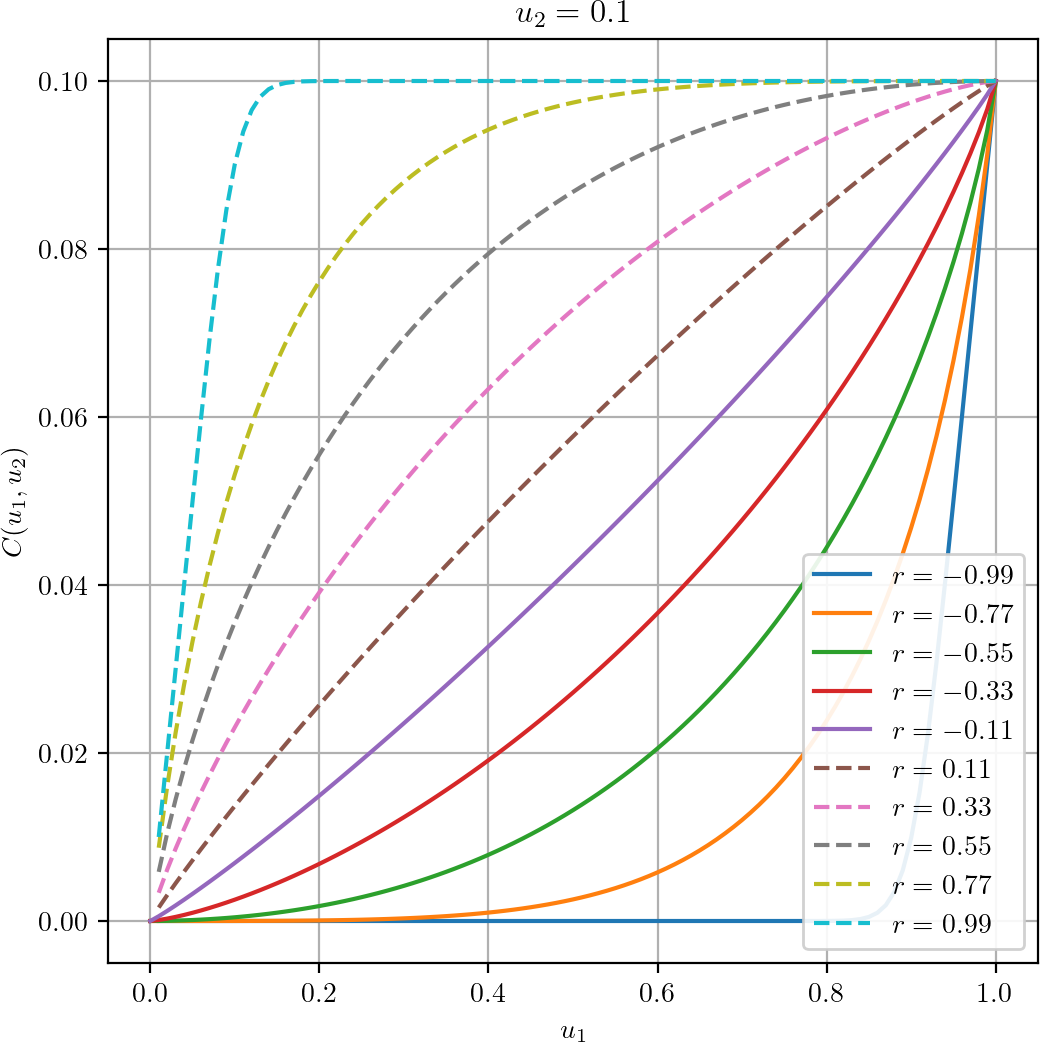
\includegraphics[width=\linewidth]{Images/Chap_2/Gaussian_copula/gaussian_copula_0.png}
    \end{subfigure}\hfill
    \begin{subfigure}{0.4\linewidth}
        \centering
        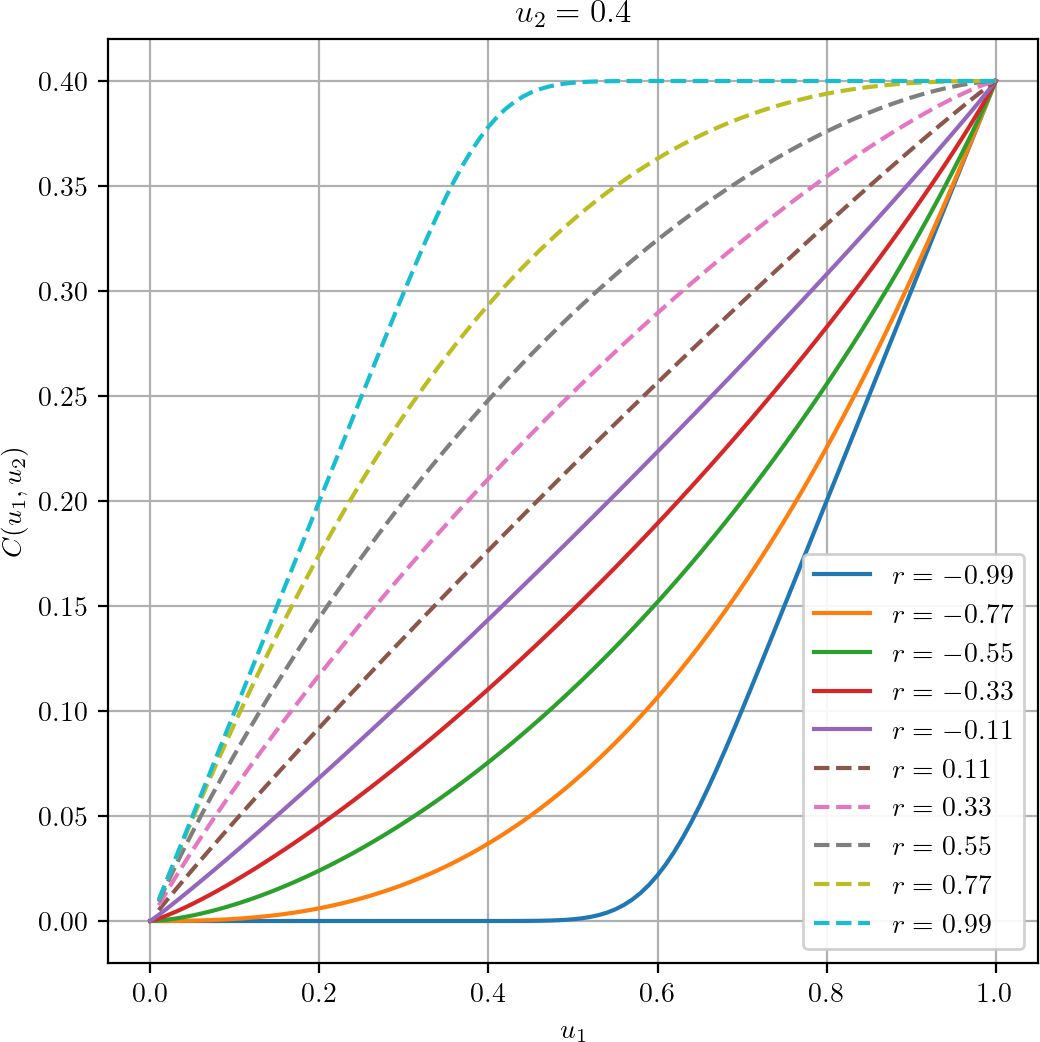
\includegraphics[width=\linewidth]{Images/Chap_2/Gaussian_copula/gaussian_copula_1.png}
    \end{subfigure}\hfill
    \begin{subfigure}{0.4\linewidth}
        \centering
        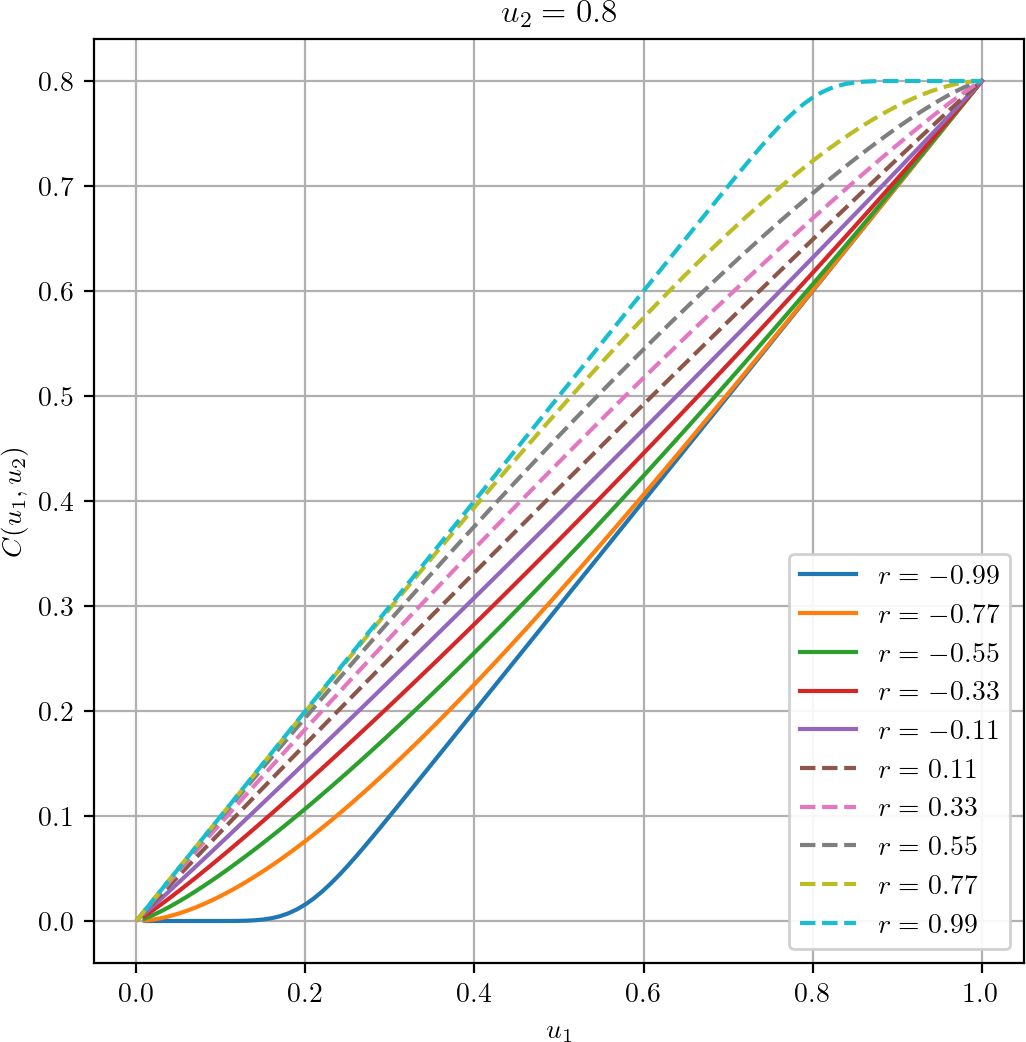
\includegraphics[width=\linewidth]{Images/Chap_2/Gaussian_copula/gaussian_copula_2.png}
    \end{subfigure}
    \caption{Gaussian 2-copulas in the direction $u_1$ for different $u_2$. Each figure present different plots for correlations $r$ between $u_1$ and $u_2$ ranging in $[-1,1]$. Solid lines represent negative correlation, while dashed lines represent positive correlations.}
    \label{fig:gaussian_copula_simu}
\end{figure}

The rest of this section will present different results regarding D-convex and D-concave copulas, leading to the main result of this section presented in proposition \ref{prop:convex_diff_hvol}.

\begin{figure}
    \centering
    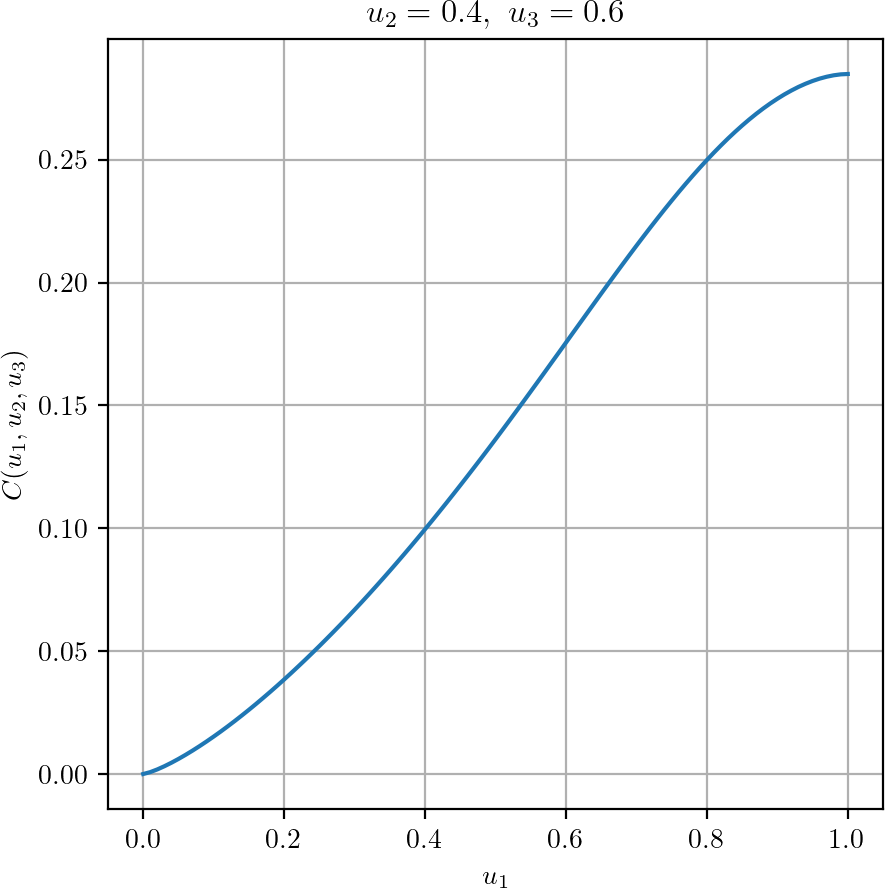
\includegraphics[width=0.5\linewidth]{Images/Chap_2/Gaussian_copula/gaussian_copula_n3.png}
    \caption{Directional cut of a Gaussian 3-copula with in the direction $u_1$, with $R=\begin{bmatrix} 1 & -0.4 & 0.7\\ -0.4 & 1 & 0.3\\ 0.7 & 0.3 & 1 \end{bmatrix}$, $u_2=0.4$ and $u_3=0.6$. The copula is neither D-convex nor D-concave}
    \label{fig:gaussian_copula_simu_n3}
\end{figure}

\begin{remark}
    All D-convex copulas $C$ are dominated by the product copula. Similarly, all D-concave copulas dominate the product copula.

    Consider a D-convex copula $C$, and let $(u_1\enum u_n)\in[0,1]^n$.
    \begin{eqnarray*}
        C(u_1\enum u_n) &=& C((1-u_1)\cdot0+u_1\cdot 1, u_2\enum u_n)\\
        &\leqslant& (1-u_1)C(0, u_2\enum u_n)+u_1C(1, u_2\enum u_n)\\
        &=& u_1C(1, u_2\enum u_n)\commanue{alors moi je laisserais le symbole $\leqslant$ et pas $=$}
    \end{eqnarray*}
    Doing the same for $u_2\enum u_n$ yields:
    \begin{eqnarray*}
        C(u_1\enum u_n) &\leqslant& u_1\dots u_nC(1\enum1) = u_1\dots u_n = C_\Pi(u_1\enum u_n)
    \end{eqnarray*}
    The proof for D-convexity is similar.
\end{remark}

\begin{proposition}\label{prop:sup_additivity}
    If $C$ is a D-convex copula, then it verifies for all $(u_1\enum u_n)\in[0,1]^n$, $(v_1\enum v_n)\in[0,1]^n$ \st $\forall i\in\opi1,n\cli$, $u_i+v_i\leqslant 1$:
    \begin{eqnarray}
        C(u_1\enum u_i+v_i\enum u_n)\geqslant& &C(u_1\enum u_i\enum u_n)\nonumber\\
        &+ &C(u_1\enum v_i\enum u_n)\label{eq:convex_sum}
    \end{eqnarray}
    Similarly, if $\forall i\in\opi1,n\cli$, $u_i-v_i\geqslant 0$, it verifies:
    \begin{eqnarray}
        C(u_1\enum u_i-v_i\enum u_n)\leqslant& &C(u_1\enum u_i\enum u_n)\nonumber\\
        &- &C(u_1\enum v_i\enum u_n)\label{eq:convex_diff}
    \end{eqnarray}
    The inequalities are reversed for D-concave copulas.
\end{proposition}

\begin{proof}
    Let $(u_1\enum u_n)\in[0,1]^n$, $(v_1\enum v_n)\in[0,1]^n$ \st $\forall i\in\opi1,n\cli$, $u_i+v_i\leqslant 1$. Let $i\in\opi1,n\cli$. Applying the definition of convexity \eqref{eq:convex_copula} with $v_i=0$ yields:
    \begin{eqnarray*}
        \forall t\in[0,1],~C(u_1\enum tu_i\enum u_n) \leqslant tC(u_1\enum u_n)
    \end{eqnarray*}
    
    Let $w_i=u_i+v_i\in ]0,1]$ (the case where $u_i=0$ or $v_i=0$ is trivial). It is possible to write $u_i=tw_i$ and $v_i=(1-t)w_i$, with $t=\frac{u_i}{w_i}\in[0,1]$. Then it holds that:
    \begin{eqnarray*}
            C(u_1\enum u_i\enum u_n) =& C(u_1\enum tw_i\enum u_n) &\leqslant tC(u_1\enum w_i\enum u_n)\\
            C(u_1\enum v_i\enum u_n) =& C(u_1\enum (1-t)w_i\enum u_n) &\leqslant (1-t)C(u_1\enum w_i\enum u_n)
    \end{eqnarray*}
    Summing the above equations yields:
    \begin{eqnarray*}
        C(u_1\enum u_i\enum u_n) + C(u_1\enum v_i\enum u_n) &\leqslant& C(u_1\enum w_i\enum u_n)\\
        &\leqslant& C(u_1\enum u_i+v_i\enum u_n)
    \end{eqnarray*}
    which proves \cref{eq:convex_sum}.

    Let $w_i=u_i-v_i\in [0,1]$, clearly $w_i+v_i\leqslant1$. Using \cref{eq:convex_sum}, it holds that:
    \begin{align*}
        &C(u_1\enum w_i\enum u_n) + C(u_1\enum v_i\enum u_n) &\leqslant~&C(u_1\enum w_i+v_i\enum u_n)\\
        \Leftrightarrow~ &C(u_1\enum w_i\enum u_n) &\leqslant~&C(u_1\enum w_i+v_i\enum u_n)\\
        &&&-C(u_1\enum v_i\enum u_n)\\
        \Leftrightarrow~ &C(u_1\enum u_i-v_i\enum u_n) &\leqslant~&C(u_1\enum u_i\enum u_n)\\
        &&&-C(u_1\enum v_i\enum u_n)
    \end{align*}
    which proves \cref{eq:convex_diff}.
\end{proof} 

\begin{proposition}\label{prop:convex_diff_hvol}
    If $C$ is a D-convex copula, then it verifies for all $(u_1\enum u_n)\in[0,1]^n$, $(v_1\enum v_n)\in[0,1]^n$ \st $\forall i\in\opi1,n\cli$, $u_i-v_i\geqslant 0$:
    \begin{eqnarray}
        C(u_1-v_1\enum u_i-v_i\enum u_n-v_n)\leqslant& &H^{u_1\enum u_i\enum u_n}_{v_1\enum v_i\enum v_n}\label{eq:convex_diff_hvol}
    \end{eqnarray}
    where $H$ is the H-volume of $C$. The inequality is reversed for D-concave copulas.
\end{proposition}

\begin{proof}
    The result is straightforward by induction using \cref{eq:convex_diff}.
\end{proof}

\subsection{Sampling from a Copula}\label{sec:sampling_copula}
As a copula represent the CDF of a multivariate random variable, it is possible to sample from it. This section details a method for sampling from copulas in general, and a special method for sampling from Gaussian copulas. \commanu{question béotien: est ce que ca te sert après ou idem c'est pour la théorie. Tu l'as fait de mettre une phrase de contexte par rapport à ta thèse, peut etre bien ici aussi pour "sampling from copula"} For simplicity, let us first present a method for sampling in the case $n=2$. Given a copula $C$, and two CDF $F_X$ and $F_Y$, a method to generate a pair of observations $(x, y)$ from a joint CDF $C(F_X, F_Y)$ is the following:

\begin{itemize}
    \item Sample two independent samples $u_1, u_2$ from a uniform distribution on [0,1]
    \item Set $v=\partial C^{-1}(u_2)$ where $\partial C^{-1}$ is the quasi-inverse of the partial derivative of $C$ regarding its first variable (which exists almost everywhere and is invertible).
    \item We now have a sample $(u_1, v)$ from a multivariate random. Its marginals follow a uniform distribution on $[0,1]$, and its associated copula is $C$.
    \item The desired pair is $(x_1,x_2) = (F^{-1}_X(u_1), F^{-1}_Y(v))$, with $F_X^{-1}$, $F_Y^{-1}$ being the quasi-inverses of the marginals CDFs.
\end{itemize}

We do not present the $n$-dimensional general case here as it is a bit more complex, but it can be found in \cite{cherubini_copula_2004}. However, drawing samples from a Gaussian $n$-copula with a correlation matrix $R$ are simpler to obtain:
\begin{itemize}
    \item Compute the Cholesky decomposition $A$ of the correlation matrix $R$
    \item Draw $n$ independent random samples $u=(u_1\enum u_n)'$ from $\mathcal{N}(0,1)$, where $\mathcal{N}$ is the normal distribution.
    \item Set $v=Au$
    \item Set $w_k=\Phi(v_k)$ where $\Phi$ is the univariate normal cumulative distribution function
    \item The desired draw is $(x_1\enum x_n)=(F^{-1}_1(w_1)\enum F^{-1}_n(w_n))$ with $F_i^{-1}$, being the quasi-inverse of the $i$-th marginal CDF.
\end{itemize}
\commanue{Alors il manque une conclusion un truc, là ça termine un peu de manière abrupte, transition donc ;)}\comloic{+1 ne serait ce qu'un badge ou un remerciement pour avoir atteint la fin du chapitre ;-) (avec un encouragement avant le prochain)... là je me sens devant le chapitre 3 un peu comme devant le panneau 10km du sommet à la moitié du tourmalet quand tu sais que la haut c'est encore bien raide. J'hésite entre poser le pied à terre, enfiler des tongues et lire le chapitre 4 tranquilou sur une place de café au risque de me tromper de direction en repartant et plus jamais trouver le courage de faire le 3, ou bien continuer avec acharnement sur le 3 juste par fierté en faire une histoire entre les copules et moi. Le truc c'est que s'il y a pas un monument une boutade ou quoi à la fin du chapitre 3 ça va pas être super gratifiant ^^'}


\pagebreak
\blankpage
    
    \setkeys{Gin}{draft=true}
    \chapter{Using Copulas to Join Credal Sets}\label{chap:joining_credal_sets}
In the presence of multiple uncertain variables, the question of how to join them arises. Using probability distributions, the usual method for joining probability distributions is to use copulas (\Cref{sec:copulas}). Indeed, \hyperref[theorem:sklar]{Sklar's Theorem} provides a well-defined way of uniquely joining multiple continuous \acrshort{cdf} with a copula. However, this is no longer true when adding imprecision to the models, as there are multiple ways of specifying the dependency between imprecise models using a copula. \Cref{sec:robust_method,sec:joint_mass,sec:aggregation_method} present three different ways of joining credal sets using a copula. Those three methods are not equivalent. We thus explore their similarities and differences in \Cref{sec:inclusions_between_methods}. Methods will be used to join possibility distributions to propagate the uncertainty in \Cref{chap:propagating}. 

\section{Methods for Joining Credal Sets with Copulas}\label{sec:methods_for_joining_credal_sets}
This section will use copulas, introduced in \Cref{sec:copulas}, to join imprecise models in three different ways. The way we prove the existence of copulas and their usage with \hyperref[theorem:sklar]{Sklar's Theorem} was based on \acrshort{cdf}s \cite{nelsen_introduction_2006}. However, the \acrshort{ip} model closest to \acrshort{cdf}s, p-boxes from \Cref{sec:pboxes}, does not allow representing every credal set as seen in \Cref{fig:diagram_IP}. When working with marginals modeled by \acrlong{ip}, we will thus define different methods for using \acrshort{ip} with copulas. The first approach in \Cref{sec:robust_method} maintains the classical interpretation of a copula found in \hyperref[theorem:sklar]{Sklar's Theorem}. The multivariate credal set obtained with this method is however hard to handle computationally. A similar approach using only the product copula can be already be found in \cite{couso_survey_2000}. The second approach in \Cref{sec:joint_mass} takes some distances with the classical interpretation of a copula, but is easier to handle computationally. It is based on previous work detailed in \cite{ferson_dependence_2004}. Finally, we introduce a third approach in \Cref{sec:aggregation_method}, which completely abandons \hyperref[theorem:sklar]{Sklar's Theorem} interpretation, but is very easy to handle. Inclusion relationships between those three approaches are explored in \Cref{sec:inclusions_between_methods}, in order to determine which is an approximation of the other.

We consider here $n\in\mathbb{N}^*$ uncertain variables $(X_i)_{1\leqslant i\leqslant n}$ taking values respectively in a totally ordered finite space $\X_i$. The index $i$ will usually refer to the $i$-th random variable (or random set). We denote $\M_i$ as the credal set representing the uncertainty of $X_i$, and $C$ a $n$-copula. We also suppose that $\M_i$ the lower bound of $\M_i$ is defined by a belief function. Focal sets of belief functions will be noted $a^i_k$, where $k$ refers to the $k$-th focal set, if they are numbered. We also note $\bigsqcup$ the union of disjoint elements. Finally, we must introduce the concept of cylindrical sets, used to specify definition domains of various mappings. 
\begin{definition}[Cylindrical sets]
    Let $\X_1 \enum \X_n$ be $n$ sets and let $\X=\X_1\tdt\X_n$ be the Cartesian product of $\X_1 \enum \X_n$. We call a cylindrical (or cylinder) set $X$ of $\X$ a set which can be written as a Cartesian product of elements of $\X_1 \enum \X_n$, \ie:
    \begin{equation}
        X\subseteq\X \text{ is cylindrical} ~\Leftrightarrow~ \exists (X_1 \enum X_n),~\st~X=X_1\tdt X_n \label{eq:cylindrical_sets}
    \end{equation}
\end{definition}

\subsection{Point-wise Aggregation}\label{sec:robust_method}
A first way of creating a joint credal set is to first consider every precise marginal within each marginal credal sets $\M_i$. We then use \hyperref[theorem:sklar]{Sklar's Theorem} with the copula $C$ to create a precise multivariate \acrshort{cdf}. The set of all resulting \acrshort{cdf}s is as follows:
\begin{align}\label{eq:robust_ancestor}
    \mathcal{S}(C,& ~\M_i) = \nonumber\\
    &\{F~|~\forall x_i \in \X_i,~F_i\in\M_i, ~ F(x_1 \enum x_n) = C(F_1(x_1) \enum F_n(x_n))\}
\end{align}

This set is not guaranteed to be convex \cite{schmelzer_random_2023}. We thus define the joint credal set as the convex hull $\M_{robust}$ of $\mathcal{S}$

\begin{definition}[Robust Credal Set]\label{def:robust_credal_set}
    We define the robust credal set obtained by joining $n$ marginal credal sets $\M_i$ and a copula $C$ as:
    \begin{eqnarray}\label{eq:robust_set}
        \M_{robust}(C,\M_i) = CH(\{C(F_1 \enum F_n),~F_i\in\M_i \})
    \end{eqnarray}
    where $CH$ is the convex hull presented in \Cref{def:convex_hull}.
\end{definition}

We refer to this joint credal set as $\M_{robust}(C,\M_i)$ as it contains every element of the marginal credal sets with copula $C$ as their dependency model. We will omit ``$(C,\M_i)$'' when there is no confusion possible to avoid using heavy notations. As we take the convex hull of $\mathcal{S}$, it is interesting to notice that it can contain additional multivariate \acrshort{cdf}s that do not possess the copula $C$ as their dependency model, as seen in \Cref{ex:robust_credal_set}. This credal set is usually hard to compute for events that are not Cartesian products of marginal cumulative events. Indeed, copula being non-linear operators, there is no reason that their point-wise application would preserve convexity. 

\begin{example}\label{ex:robust_credal_set}
Consider two coins, with their associated random variable $X_1$ and $X_2$ taking values in $\X_1=\X_2=\{heads, ~tails\}$. The uncertainty of each random variable is represented by the following mass distribution function $m_1$ and $m_2$:\newline\medskip
\begin{minipage}{0.5\linewidth}
\begin{align*}
    &m_1(heads)=0.4 \\
    &m_1(tails) = 0.4\\
    &m_1(\X_1)=0.2
\end{align*}
\end{minipage}
\begin{minipage}{0.5\linewidth}
\begin{align*}
    &m_2(heads)=0.4\\
    &m_2(tails) = 0.5\\
    &m_2(\X_2)=0.1
\end{align*}
\end{minipage}\bigskip\newline
The credal sets $\M_1$ and $\M_2$ associated with $X_1$ and $X_2$ are therefore composed of all the probabilities $P_1\in\M_1$ and $P_2\in\M_2$ verifying:\newline\medskip
\begin{minipage}{0.5\linewidth}
\begin{align*}
    0.4 ~\leqslant~ &P_1(heads) ~\leqslant~ 0.6 \\
    0.4 ~\leqslant~ &P_1(tails) ~\leqslant~ 0.6
\end{align*}
\end{minipage}
\begin{minipage}{0.5\linewidth}
\begin{align*}
    0.4 ~\leqslant~ &P_2(heads) ~\leqslant~ 0.5 \\
    0.5 ~\leqslant~ &P_2(tails) ~\leqslant~ 0.6
\end{align*}
\end{minipage}\bigskip\newline
If we assume we throw the two coins independently, then their dependency can be modeled by the product copula $C_\Pi(u,v)=u\cdot v$.

The robust credal set $\M_{robust}$ obtained by joining $\M_1$ and $\M_2$ with $C_\Pi$ will therefore be the convex hull of the set:
\begin{align*}
    \{P~|~\forall P_1\in\M_1, P_2\in\M_2,~&\forall (x_1,x_2)\in\X_1\times\X_2,\\
    ~&P(x_1, x_2) = P_1(x_1)\cdot P_2(x_2)~\}
\end{align*}
In this specific case the bounds of $P\in\M_{robust}$ on cylindrical sets are quite straightforward because we consider binary random variables and the product copula:\newline\medskip
\begin{minipage}{0.5\linewidth}
\begin{align*}
    0.16 ~\leqslant~ &P(heads, heads) ~\leqslant~ 0.3 \\
    0.2 ~\leqslant~ &P(heads, tails) ~\leqslant~ 0.36
\end{align*}
\end{minipage}
\begin{minipage}{0.5\linewidth}
\begin{align*}
    0.2 ~\leqslant~ &P(tails, tails) ~\leqslant~ 0.36 \\
    0.16 ~\leqslant~ &P(tails, heads) ~\leqslant~ 0.3
\end{align*}
\end{minipage}\bigskip\newline
Now, let us exhibit a probability from $\M_{robust}$ that does not have $C_\Pi$ as its dependency model. Consider the following marginal probabilities $P_1,P_1'\in\M_1$ and $P_2,P_2'\in\M_2$:\newline\medskip
\begin{minipage}{0.5\linewidth}
\begin{align*}
    &P_1(heads)=0.4 \\
    &P_1'(heads)=0.6
\end{align*}
\end{minipage}
\begin{minipage}{0.5\linewidth}
\begin{align*}
    &P_2(heads)=0.4 \\
    &P_2'(heads)=0.5
\end{align*}
\end{minipage}\bigskip\newline
Then $P=P_1\cdot P_2$ and $P'=P_1'\cdot P_2'$ both belong in $\M_{robust}$, and the convex mixture $P_{0.5}=0.5\cdot P+0.5\cdot P'$ is also in $\M_{robust}$.
We will compute the value of $P_{0.5}(heads, heads)$ and show that it does not equal to the product of its marginals:
\begin{align*}
    P_{0.5}(heads, heads) &= 0.5\cdot P(heads, heads)+0.5\cdot P'(heads, heads)\\
    &= 0.5\cdot P_1(heads)\cdot P_2(heads)+0.5\cdot P_1'(heads)\cdot P_2'(heads)\\
    &= 0.5\cdot 0.4\cdot 0.4+0.5\cdot 0.6\cdot 0.5\\
    &=0.08+0.15 = 0.23
\end{align*}
\begin{align*}
    P_{0.5}(heads, \X_2) &= 0.5\cdot P_1(heads)\cdot P_2(\X_2) + 0.5\cdot P_1'(heads)\cdot P_2'(\X_2)\\
    &= 0.5\cdot 0.4 + 0.5\cdot 0.6\\
    &= 0.2+0.3 = 0.5\\
    P_{0.5}(\X_1, heads) &= 0.5\cdot P_1(\X_1)\cdot P_2(heads) + 0.5\cdot P_1'(\X_1)\cdot P_2'(heads)\\
    &= 0.5\cdot 0.4 + 0.5\cdot 0.5\\
    &= 0.2+0.25 = 0.45
\end{align*}
The product of the marginals on heads is therefore equal to
\begin{align*}
    P_{0.5}(heads, \X_2)\cdot P_{0.5}(\X_1, heads)&= 0.5\cdot0.45\\
    &=0.225\\
    &\neq 0.23 = P_{0.5}(heads, heads)
\end{align*}
therefore $P_{0.5}$ belongs to $\M_{robust}$ but does not have $C_\Pi$ as its copula.
\end{example}

\begin{remark}
	Due to the convex hull, we can both consider $\M_{robust}$ as only containing probabilities on the set $\X=\X_1\tdt\X_n$ and containing probabilities on $2^\X$. This applies to the other credal sets as well. We will consider the latter, though the former has been considered in the literature (for instance \cite{schmelzer_characterizing_2012, schmelzer_random_2023}). To insist on which marginal events we consider, we will sometimes write $P(a^1, a^2)$ instead of $P(a^1\times a^2)$, even though this notation suggests that $P$ is defined on $\X$ and not $2^\X$. 
\end{remark}

\Cref{fig:schema_m_robust} represents a schematic of $\M_{robust}$ is obtained. First, two samples $F_1$ and $F_2$ (represented by ``$+$'' signs) are sampled from the marginals credal sets $\M_1$ and $\M_2$. They are then joined using the copula $C$ to create a multivariate \acrshort{cdf} represented by a ``x'' sign. This process is then reproduced for every combination of samples in the marginal credal sets and $\M_{robust}$ is the convex hull of the set of samples.
\begin{figure}[!ht]
    \centering
    \begin{tikzpicture}[scale=1]
        \draw [red, line width=0.4mm] plot [smooth cycle, tension=1.1] coordinates {(5,1) (7,2) (5,3) (3,2)};
        \draw [cyan, line width=0.4mm] plot [smooth cycle, tension=2] coordinates {(0,4) (1,3) (2,4) (1,5)};
        
        \draw (7.5, 2) node (Belx) {\color{red}$\M_1$};
        \draw (1, 5.5) node (Bely) {\color{cyan}$\M_2$};
        
        \draw (4.2, 2.2) node (a) {\textbf{+}};
        \draw (4.5, 1.9) node (A) {$F_1$};
        \draw [gray] (5, 1.2) node (+) {+};
        \draw [gray] (6.8, 2) node (+) {+};
        \draw [gray] (5, 2.8) node (+) {+};
        \draw [gray] (3.2, 2) node (+) {+};
        
        
        \draw (1.3, 4) node (b) {\textbf{+}};
        \draw (0.8, 4) node (B) {$F_2$};
        \draw [gray] (0.2, 3.2) node (+) {+};
        \draw [gray] (0.2, 4.8) node (+) {+};
        \draw [gray] (1.8, 3.2) node (+) {+};
        \draw [gray] (1.8, 4.8) node (+) {+};
        
        \draw (4, 4.5) node (c) {x};
        \draw (5.2, 4.5) node (C) {$C(F_1,~F_2)$};
        \draw[->] (a) to [bend right] node[midway, left, inner sep=0.5cm] {$C$}(c);
        \draw[->] (b) to [bend left] (c);
        
        \draw [gray] (3.8, 4.8) node (c) {x};
        \draw [gray] (6.8, 4.7) node (c) {x};
        \draw [gray] (5.7, 5.7) node (c) {x};
        \draw [gray] (6.3, 3.5) node (c) {x};
        \draw [gray] (5.5, 4) node (c) {x};
        
        \draw [violet, dashed, line width=0.4mm] plot [smooth cycle,tension=1.2] coordinates {(3.7, 4.2) (5, 4) (6.5, 3.5) (6.5, 5.5) (4.3, 5.4)};
        
        \draw (8, 5) node (robust) {\color{violet}{$\M_{robust}$}};
    \end{tikzpicture}
    \caption{Schematic representation of $\M_{robust}$}\label{fig:schema_m_robust}
\end{figure}

\subsection{Copula Applied to Cumulative Mass Functions}\label{sec:joint_mass}
In this section, we will present another way of creating a joint credal set from multiple marginal ones. Consider the same copula $C$ as before and the same marginal credal sets $\M_i$. Each credal set $\M_i$ is fully determined by a mass distribution function $m_i$, which is strictly positive over its $N_i$ focal sets $a^i_1 \enum a^i_{N_i}$. As described in \cite{ferson_dependence_2004}, it is possible to use the cumulative mass distribution functions as marginals of the copula to create a joint mass distribution function, granted that there is a complete ordering defined on the focal sets. Links between copulas and belief functions have been investigated in the continuous case in \cite{schmelzer_joint_2015, schmelzer_multivariate_2019}, the special case of necessity functions in \cite{schmelzer_sklars_2015} and of p-boxes in \cite{schmelzer_random_2023}.

Let us assume, without loss of generality, that the marginal focal sets are numbered according to the ordering $\preceq_i$: $a^i_1\preceq_ia^i_2\preceq_i\ldots\preceq_i a^i_{N_i}$. The idea behind this method is to replace the precise marginal \acrshort{cdf}s by cumulative masses, to keep the philosophy behind \hyperref[theorem:sklar]{Sklar's Theorem}. We thus first define the joint mass $m_C$ on the product space of focal sets as follows:

\begin{definition}[Joint Mass]\label{def:joint_mass}
    Let $m_1 \enum m_n$ be mass distribution functions over their respective power sets of $\X_1 \enum \X_n$. Assume that focal sets in each $\X_i$ are ordered and that $a_{k_i}^i$ is the $k_i$-th focal set of $m_i$ according to the chosen order. We define $m_C$ as the H-volume of copula $C$ computed over the cumulative marginal masses:
    \begin{eqnarray}\label{eq:joint_mass}
        m_C(a^1_{k_1}\tdt a^n_{k_n}) = H_{\sum_{k=0}^{k_1-1}m_1(a^1_k) \enum \sum_{k=0}^{k_n-1}m_n(a^n_k)}^{\sum_{k=0}^{k_1}m_1(a^1_k) \enum \sum_{k=0}^{k_n}m_n(a^n_k)}
    \end{eqnarray}
    with the convention that $\forall i,\, a^i_0=\emptyset$. It is not \textit{strictly} a focal set but allows dealing with the case $k_i=1$ as $m_i(a^i_0)=0$. For sets that are not of the form $a^1_{k_1}\tdt a^n_{k_n}$, the mass $m_C$ is null.
\end{definition}

\begin{proposition}
    The function $m_C$ defined in \Cref{eq:joint_mass} is a correctly defined mass distribution function over $\X$. 
\end{proposition}
\begin{proof}
    To be a mass distribution function over $\X$, $m_C$ must verify the 3 properties of \Cref{def:mass_distribution_function}.
    
    By construction, it holds that $m_C(\emptyset)=0$, and the properties of the H-volume impose that $m_C\in[0,1]$.
    
    There are multiple ways of proving that $\sum_{A\subseteq\X}m_C(A)=1$. A direct proof can be done in the case $n=2$, but the notations become quite heavy for any $n>2$. Instead, let us use the interpretation of a copula as a multivariate \acrshort{cdf}. This method will also be used in future proofs.
    
    For all \(i\in\opi 0,\, n\cli\) let $F_i$ be a \acrshort{cdf} over $[0,\, N_i]$, with $F_i(j)=\sum_{k=0}^j m_i(a_k^i)$. By \hyperref[theorem:sklar]{Sklar's Theorem}, $F=C(F_1 \enum  F_n)$ is a multivariate \acrshort{cdf} over $[0,\, N_1]\tdt[0,\, N_n]$, and $P$ its \acrshort{pdf}. Thus, it holds that $P([0,\, N_1]\tdt[0,\, N_n])=F(N_1,\ldots,N_n)=1$ and:
    \begin{eqnarray*}
        P([0, N_1]\tdt[0, N_n]) &=& P([0, ~\ldots, ~0])+\\
        &&P\left(\bigsqcup_{k_1=0}^{N_1-1}\ldots\bigsqcup_{k_n=0}^{N_n-1}\left(]k_1, k_1+1]\tdt]k_n, k_n+1]\right)\right)\\
        &=& 0 + \sum_{k_1=0}^{N_1-1}\ldots\sum_{k_n=0}^{N_n-1} P(]k_1, k_1+1]\tdt]k_n, k_n+1])\\
        && \text{(\acrshort{cdf} of a union of disjoint elements, as in \Cref{fig:Demo_CDF})}\\
        &=& \sum_{k_1=0}^{N_1-1}\ldots\sum_{k_n=0}^{N_n-1} H_{F_1(k_1) \enum F_n(k_n)}^{F_1(k_1+1) \enum F_n(k_n+1)}\\
        &=& \sum_{k_1=1}^{N_1}\ldots\sum_{k_n=1}^{N_n} H_{\sum_{k=0}^{k_1-1}m_1(a^1_k) \enum \sum_{k=0}^{k_n}m_n(a^n_k)}^{\sum_{k=0}^{k_1}m_1(a^1_k) \enum \sum_{k=0}^{k_n}m_n(a^n_k)}\\
        &=& \sum_{(a^1_{k_1}\tdt a^n_{k_n})\subseteq\X}m_C(a^1_{k_1}\tdt a^n_{k_n})
    \end{eqnarray*}
Therefore it holds that:
\begin{eqnarray}
    \sum_{A\subseteq\X}m_C(A)=\sum_{(a^1_{k_1}\tdt a^n_{k_n})\subseteq\X}m_C(a^1_{k_1}\tdt a^n_{k_n})=1
\end{eqnarray}
which proves that $m_C$ is a mass distribution function.

{\centering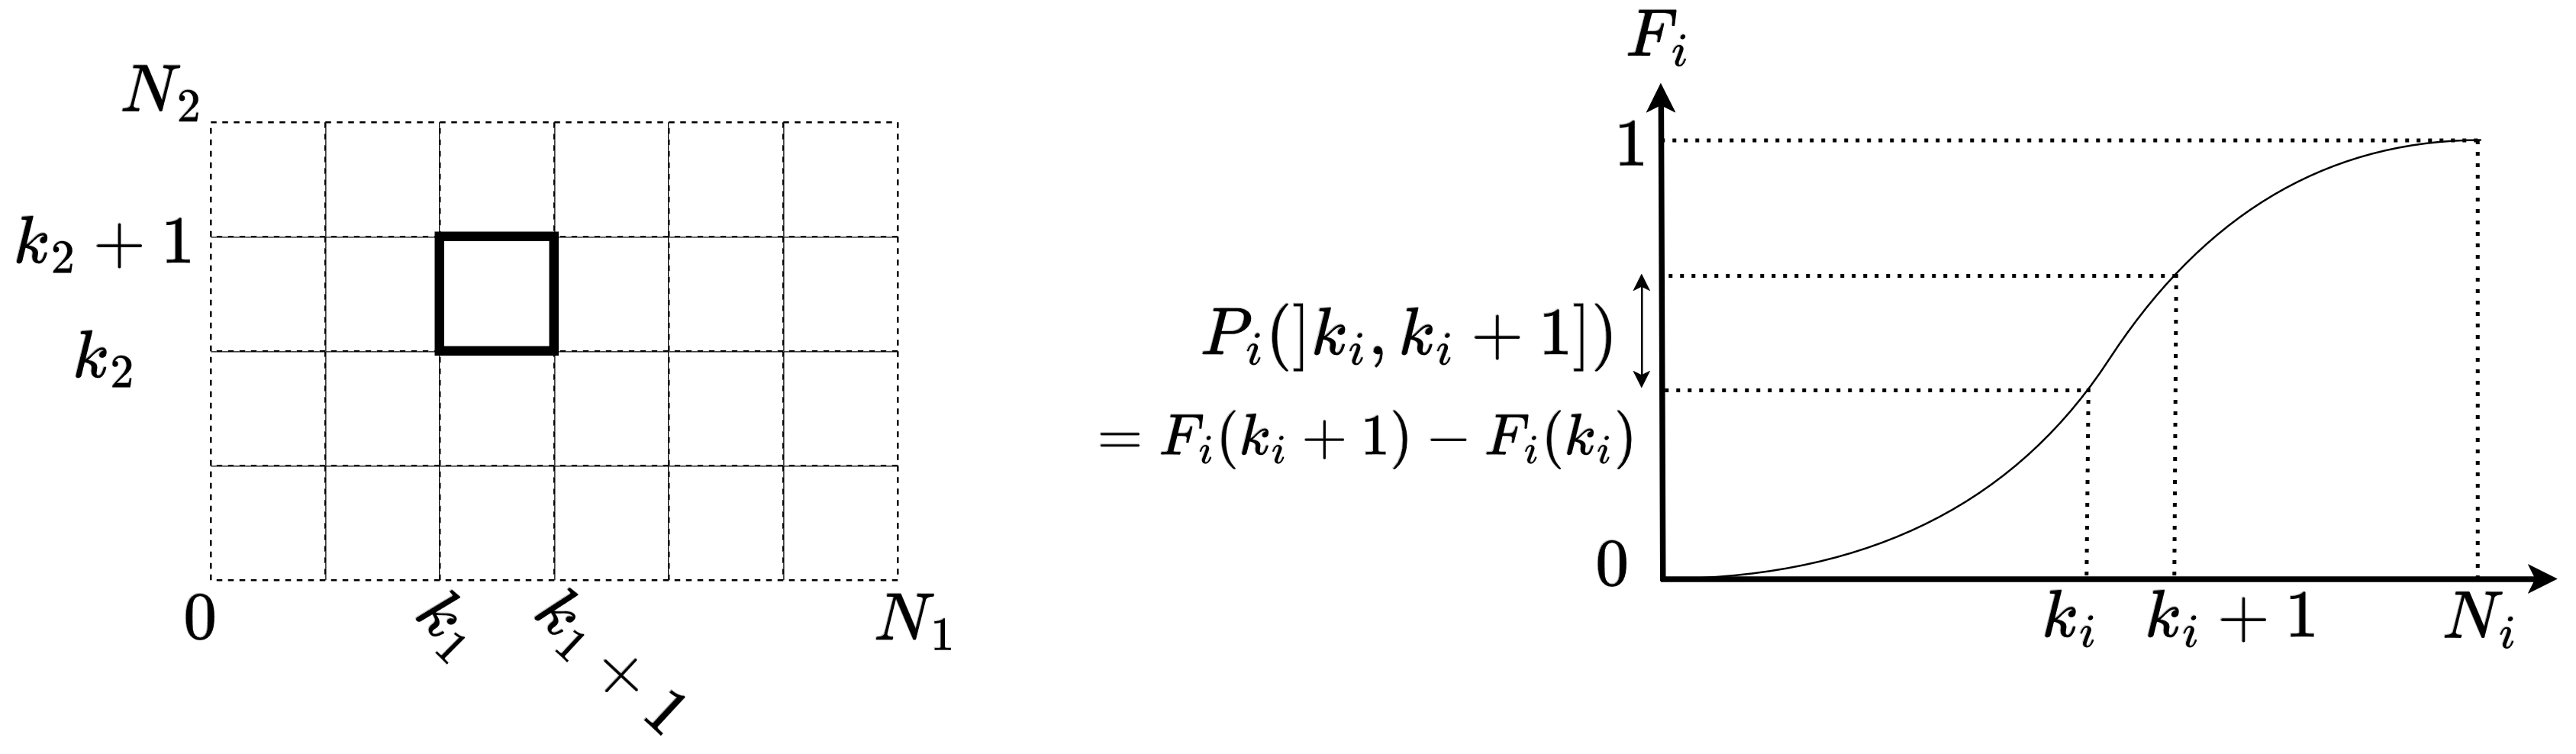
\includegraphics[width=\linewidth]{Images/Chap_3/Demo_CDF.png}\captionof{figure}{Splitting a \acrshort{cdf} into a sum of disjoint events in dimension 1}\label{fig:Demo_CDF}}\par
\end{proof}

Having defined a mass distribution function on the product space $\X$, we thus define the joint credal set $\M_{mass}$ and its belief function $\Bel_C$ as:
\begin{definition}[Joint Belief Function and its Credal Set]\label{def:cumulative_masses_credal_set}
    Let $m_C$ be the mass distribution function from \Cref{def:joint_mass}. We note $\Bel_C$ its joint belief function over the power set of $\X=\X_1\tdt \X_n$, \ie:
    \begin{align}
        \forall A\subseteq\X, \Bel_C(A)=\sum_{a\subseteq A}m_C(a)\label{eq:joint_belief}
    \end{align}
    Because $\Bel_C$ is a belief function, it defines a credal set $\M_{mass}$:
    \begin{eqnarray}
        \M_{mass}(C,\M_i) = \{~P:2^\X\rightarrow [0,1] ~|~ \forall A\subseteq\X, P(A)\geqslant \Bel_C(A)~\}\label{eq:credal_set_mass}
    \end{eqnarray}
    We only specify the lower bound $\Bel_C$ in the expression of the credal set as 
    \begin{align*}
        \Bel_C(A^c)&\leqslant P(A^c)\\
        \Leftrightarrow 1-\Pl(A) &\leqslant 1-P(A)\\
        \Pl(A) &\geqslant P(A)
    \end{align*}
\end{definition}

\Cref{fig:schema_credal_mass} presents a schematic of $\Bel_C$ similarly to what was presented with $\M_{robust}$ in \Cref{fig:schema_m_robust}: $\Bel_C$ is computed from $\Bel_1$ and $\Bel_2$. The gray ``+'' and ``X'' signs have the same position as in \Cref{fig:schema_m_robust}, which shows that $\M_{robust}$ and $\M_{mass}$ are not the same, as the copula is applied to the cumulative masses instead of being applied point-wise to every \acrshort{cdf} from marginal sets.
\begin{figure}
    \centering
    \begin{tikzpicture}[scale=1]
        \draw (7.5, 2) node (Belx) {\color{red}$\Bel_1$};
        \draw (1, 5.5) node (Bely) {\color{cyan}$\Bel_2$};
        
        \draw (5.1, 2.83) node (a) {};
        \draw (5, 4.1) node (b) {};
        \draw (1.88, 4.4) node (c) {};
        \draw (3.3, 4.8) node (d) {};
        
        \draw[->, red] (a) to [bend right] node[midway, left, inner sep=0.5cm] {} (b.south);
        \draw[->, cyan] (c) to [bend left] node[midway, left, inner sep=0.5cm] {} (d.south);
        \draw (3, 4) node (e) {$C$};
        
        \draw [red, line width=0.4mm] plot [smooth cycle, tension=1.1] coordinates {(5,1) (7,2) (5,3) (3,2)};
        \draw [cyan, line width=0.4mm] plot [smooth cycle, tension=2] coordinates {(0,4) (1,3) (2,4) (1,5)};
        \draw [violet, dashed, line width=0.4mm] plot [smooth cycle,tension=1.2] coordinates {(3.7, 3.5) (5, 4) (6.5, 4) (6.5, 5.5) (4, 6) };
        
        \draw (7.5, 4.2) node (mass) {\color{violet}$\Bel_C$};
        
        \draw [gray] (4.2, 2.2) node (+) {+};
        \draw [gray] (5, 1.2) node (+) {+};
        \draw [gray] (6.8, 2) node (+) {+};
        \draw [gray] (5, 2.8) node (+) {+};
        \draw [gray] (3.2, 2) node (+) {+};
        
        \draw [gray] (1.3, 4) node (+) {+};
        \draw [gray] (0.2, 3.2) node (+) {+};
        \draw [gray] (0.2, 4.8) node (+) {+};
        \draw [gray] (1.8, 3.2) node (+) {+};
        \draw [gray] (1.8, 4.8) node (+) {+};
        
        \draw [gray] (4, 4.5) node (x) {x};
        \draw [gray] (3.8, 4.8) node (x) {x};
        \draw [gray] (6.8, 4.7) node (x) {x};
        \draw [gray] (5.7, 5.7) node (x) {x};
        \draw [gray] (6.3, 3.5) node (x) {x};
        \draw [gray] (5.5, 4) node (x) {x};
    \end{tikzpicture}
    \caption{Schematic representation of $\M_{mass}$} \label{fig:schema_credal_mass}
\end{figure}

With this way of defining the multivariate mass, the choice of arbitrary orderings $\preceq_i$ can have a significant impact on the value of the multivariate mass function, as we will see in example \Cref{ex:joint_mass}. Those orderings will specifically be ``natural'' orderings in \Cref{sec:necessity_functions,subsec:pboxes,subsec:multiple_models}, in the sense that there exists an intuitive total ordering (inspired by the ordering of reals). When no natural ordering exists, the arbitrary choice of the ordering can greatly impact the output mass or belief functions, as illustrated by the following example.
\begin{example}\label{ex:joint_mass}
    Let us consider the same setting as \Cref{ex:robust_credal_set} with two coins, and their mass defined this time as:\newline\medskip
    \begin{minipage}{0.5\linewidth}
    	\begin{align*}
    		&m_1(heads)=0.4 \\
    		&m_1(\X_1)=0.6
    	\end{align*}
    \end{minipage}
    \begin{minipage}{0.5\linewidth}
    	\begin{align*}
    		&m_2(tails)=0.7\\
    		&m_2(\X_2)=0.3
    	\end{align*}
    \end{minipage}\bigskip\newline
   We consider the minimum copula $C(u,v)=\min(u,v)$ 
    If there is no natural ordering on the focal sets of $m_1$, we have to choose an arbitrary one:\par
    $\bullet$ If "$\{heads\}\preceq_1 \X_1$" and "$\{tails\}\preceq_2\X_2$" are the arbitrary orderings, then
    \begin{eqnarray*}
        \Bel_C(heads,tails) &=& m_C(heads,tails)\\
        &=&C\left(m_1(heads),~m_2(tails)\right)\\
        &=& \min(0.4,0.7)\\
        &=&0.4
    \end{eqnarray*}\par
    $\bullet$ If "$\X_1\preceq_1 \{heads\}$" is the arbitrary order, then
    \begin{eqnarray*}
        \Bel_C(heads,tails) &=& m_C(heads,tails)\\
        &=&C\left(1,~m_2(tails)\right) - C\left(m_1(\X_1),~m_2(tails)\right)\\
        &=& m_2(tails) -\min(0.6,~0.7)\\
        &=& 0.1
    \end{eqnarray*}
    This illustrates that different orderings lead to different masses and thus to different credal sets.
\end{example}

\begin{remark}
    One reason why $\M_{robust}$ is usually different from $\M_{mass}$ is mainly because the ordering on focal sets can greatly differ from the ordering on reals. Consider for instance the minimum copula already presented in \Cref{ex:copulas}:
    \begin{itemize}
        \item In the precise setting, the minimum copula associates the highest probabilities to events with similar values (high-high or low-low), and the lowest probabilities to events with opposite values (low-high).
        \item In the imprecise setting, the concept of high or low values for focal sets does not usually exist. We thus replace it by an ordering $\preceq$ on focal sets, determining which set is considered ``low'' and which is ``high'' (regardless of the real values actually contained in the set). The minimum copula then associates the highest mass to joint focal sets with similar ``values'' in the sense of the ordering $\preceq$, and the lowest mass to sets with opposite values in the sense of the ordering $\preceq$. For instance, in the bivariate case, with marginal focal sets $a_1^1\preceq_1 a_2^1$ and $a^2_1\preceq_2 a^2_2$, using the minimum copula will assign high masses to $a^1_1\times a^2_1$ and $a^1_2\times a^2_2$ and low masses to $a^1_1\times a^2_2$ and $a^1_2\times a^2_1$.
    \end{itemize}
    Assigning a high mass to sets containing both low and high values at the same time is something that would not occur in the precise case, but is possible in the imprecise case. This explains a source of the difference between credal sets $\M_{mass}$ and $\M_{robust}$. 
\end{remark}

We saw that $\M_{robust}$ and $\M_{mass}$ can be different credal sets. However, because $\M_{robust}$ is difficult to compute, it would be interesting to still use $\M_{mass}$ to approximate it, \ie to verify that $\M_{robust}\subseteq\M_{mass}$ (outer approximation) or $\M_{mass}\subseteq\M_{robust}$ (inner approximation). In \Cref{ex:mass_values}, we show that there is in general no reason for such a relation to exist. Furthermore, if we found an ordering allowing this relationship, then this ordering is copula dependent, as changing the copula might break the inclusion. 
\begin{example}\label{ex:mass_values}
    Consider the following setting:
    \begin{itemize}
        \item We consider two spaces $\X_1=\X_2=\{1,~2,~3\}$
        \item We consider two (identical) mass distribution functions $m_1$, $m_2$, each respectively possessing two focal sets $\{2\}$ and $\{1,3\}$.
        \item $m_1(\{2\}) = m_1(\{1,~3\}) = m_2(\{2\})= m_2(\{1,~3\}) = 0.5$
        \item We want to join the credal sets induced by the mass functions using the minimum copula.
    \end{itemize}
    We will compute the bounds of $\M_{mass}$ and $\M_{robust}$ to compare them. The marginals masses being identical and the copula being symmetrical, many results can be obtained by symmetry.
    
    Let us first compute the bounds of $\M_{robust}$. Marginal masses $m_1$  and $m_2$ imposes that each marginal probability $P_1\in\M_1$ will verify:
    \begin{align*}
        \Bel_1(\{2\}) \leqslant &P_1(\{2\}) \leqslant \Pl_1(\{2\})\\
        0.5 = \sum_{a\subseteq\{2\}}m_1(a) \leqslant &P_1(\{2\}) \leqslant \sum_{a\cap\{2\}\neq\emptyset}m_1(a) = 0.5
    \end{align*}
    The same result holds for $\{1,~3\}$. We therefore have:
    \begin{align*}
        &P_1(2)=0.5\\
        &P_1(1)+P_1(3)=0.5\\
        &0\leqslant P_1(1)\leqslant 0.5\\
        &0\leqslant P_1(3)\leqslant 0.5
    \end{align*}
    And we can compute the same for $m_2$. Looking at those equations, we can deduce that every $P\in\M_{robust}$ with marginals $P_1,P_2$ verifies for events  $\{1\}\times\{1\}$ and $\{1,2\}\times\{1,2\}$:
    \begin{align*}
    	&P(\{1\},~ \{1\}) = \min(P_1(1), P_2(1))\\
        \implies 0 = \min(0, 0)  \leqslant ~&P(\{1\},~ \{1\}) ~\leqslant \min(0.5, 0.5) = 0.5\\
        &P(\{1, ~2\},~ \{1, ~2\}) = \min(P_1(\{1, ~2\}), P_2(\{1, ~2\}))\\
        \implies 0.5 = \min(0+0.5, 0.5+0) \leqslant ~&P(\{1, ~2\},~ \{1, ~2\}) ~\leqslant min(0.5+0.5, 0.5+0.5)=1
    \end{align*}
    
    Let us now compute the bounds of $\M_{mass}$. Choosing an ordering between $\{1, ~3\}$ and $\{2\}$ is not intuitive. Assume that there is a reason which encourages us to choose different orderings for the focal sets of $m_1$ and for those of $m_2$, so that $\{1,~3\} \preceq_1 \{2\}$ and $\{2\} \preceq_2 \{1,~3\}$. In this case, using \Cref{eq:joint_mass} it holds that:
    \begin{align*}
        m_C(\{1, ~3\}, \{2\}) =& ~\min(0.5, ~0.5)\\
        =& ~0.5\\
        m_C(\{2\}, \{1, ~3\}) =& ~\min(1, ~1) - \min(0.5, ~1)\\
        & - \min(1, ~0.5) + \min(0.5, ~0.5)\\
        =& ~0.5\\
        m_C(\{2\}, \{2\}) =& ~0\\
        m_C(\{1, ~3\}, \{1, ~3\}) =& ~0
    \end{align*}
    Thus every probability $P\in\M_{mass}$ will verify:
    \begin{align*}
    	\Bel_C(\{1\},~ \{1\}) \leqslant ~&P(\{1\},~ \{1\})  ~\leqslant \Pl(\{1\},~ \{1\}) \\
    	\Leftrightarrow\sum_{a\subseteq(\{1\}\times \{1\})}m_C(a)\leqslant ~&P(\{1\},~ \{1\})  ~\leqslant\sum_{a\cap(\{1\}\times \{1\})\neq\emptyset}m_C(a)\\
        \Leftrightarrow 0 \leqslant ~&P(\{1\},~ \{1\}) ~ \leqslant 0
    \end{align*}
    and
     \begin{align*}
        \Bel_C(\{1, ~2\},~ \{1, ~2\}) \leqslant ~&P(\{1, ~2\},~ \{1, ~2\})  ~\leqslant \Pl(\{1, ~2\},~ \{1, ~2\}) \\
        \Leftrightarrow\sum_{a\subseteq(\{1, ~2\},~ \{1, ~2\})}m_C(a)\leqslant ~&P(\{1, ~2\},~ \{1, ~2\})  ~\leqslant\sum_{a\cap(\{1, ~2\},~ \{1, ~2\})\neq\emptyset}m_C(a)\\
        \Leftrightarrow 0 \leqslant ~&P(\{1, ~2\},~ \{1, ~2\})~ \leqslant 1
    \end{align*}
 
    Looking at the bounds of $\M_{mass}$ and $\M_{robust}$ on cumulative event $\{1\}\times\{1\}$, we can see that $\overline{P}_{robust}(\{1\}, \{1\}) > \Pl(\{1\}, \{1\}))$ and thus $\M_{robust}\not\subseteq \M_{mass}$.
    Looking at the bounds on $\{1,2\}\times\{1,2\}$, we can see that $\low_{robust}(\{1, ~2\},~ \{1, ~2\}) > \Bel_C(\{1, ~2\},~ \{1, ~2\})$ and thus $\M_{mass}\not\subseteq \M_{robust}$.
    
    \begin{remark}
        The bounds of $\M_{mass}$ depend both on the ordering and the copula used. Therefore, if an ordering exists such that $\M_{robust}\subseteq\M_{mass}$ or $\M_{mass}\subseteq\M_{robust}$, then this ordering is not guaranteed to keep the inclusion relationship using a different copula.
    \end{remark}
\end{example}

We considered until now that an ordering has to be chosen arbitrarily. However, special cases of belief functions exhibit a natural ordering on their focal sets, for instance p-boxes and possibilities. Those special cases will be explored in \Cref{sec:inclusions_between_methods}.

\subsection{Copulas Applied to Belief Functions}\label{sec:aggregation_method}
Another way of joining credal sets with a copula is by directly applying the copula to their lower envelope $\low_i$ for every event:
\begin{definition}[Aggregated Credal Set]\label{def:aggregation_credal_set}
    Given a copula $C$ and $n$ marginal credal sets whose lower probabilities are $\low_1 \enum \low_n$, we define the credal set $\M_{agg}$ over the power set of $\X=\X_1\tdt X_n$ as:
    \begin{eqnarray}
        \M_{agg} = CH(\{P ~|~\forall A_i\subseteq\X_i, P(A_1 \enum  A_n)\geqslant C(\low_1(A_1) \enum \low_n(A_n))\})\nonumber\\
        \,\label{eq:copula_on_lower_proba}
    \end{eqnarray}
    where $CH$ is the convex hull from \Cref{def:convex_hull}.
\end{definition}

Contrary to $\M_{mass}$ or $\M_{robust}$, constraints on this set only occur on Cartesian products in $\X$. We thus take the convex hull for extending its definition to every event in $2^\X$. We denote this credal set as $\M_{agg}$ because it uses the copula solely as an aggregation operator, without conserving the meaning associated with copulas by \hyperref[theorem:sklar]{Sklar's Theorem}. In this regard, $\M_{agg}$ has less meaning than $\M_{robust}$ or $\M_{mass}$, but presents the advantage of being easier to compute on cylindrical sets. \Cref{fig:meaning_computation} sums up the performances of the different methods in terms of computation cost and meaningfulness.

\begin{figure}[!hb]
    \centering
    \begin{tikzpicture}[scale=1]
        \draw (0, 0) node (a) {};
        \draw (10, 0) node (b) {};
        \draw (0, 1.5) node (c) {};
        \draw (10, 1.5) node (d) {};
        
        \draw[->, ultra thick, darkgray] (a) to node[midway, left, inner sep=0.5cm] {} (b);
        \draw[->, ultra thick, darkgray] (d) to node[midway, left, inner sep=0.5cm] {} (c);
        
        \draw [darkgray] (9, -0.5) node (z) {\small Easy to compute};
        \draw [darkgray] (0, 2) node (z) {\small Meaningful};
        
        \draw (9, 0.75) node (z) {$\M_{agg}$};
        \draw (5.65, 0.75) node (z) {$\M_{mass}$};
        \draw (2, 0.75) node (z) {$\M_{robust}$};
    \end{tikzpicture}
    \caption{Comparing different methods of joining credal sets with a copula.}
    \label{fig:meaning_computation}
\end{figure}

In general, applying the copula directly to the lower probabilities as in \eqref{eq:copula_on_lower_proba} does not produce a coherent lower probability inducing a non-empty credal set (see \Cref{def:coherence_sure_loss}). For instance, let us consider $\X_1 = \X_2 = \{1, 2\}$, two lower previsions $\low_1$ and $\low_2$ such that $\low_1(\{1\}) = \low_1(\{2\}) = \low_2(\{1\}) = \low_2(\{2\}) = 0.5$. Joining those two lower probabilities using the minimum copula $C(u,v)=\min(u,v)$ gives a mapping $\low$ which induces an empty credal set, as presented in \Cref{tab:non_coherent_lower}. Indeed, no probabilities can satisfy all these constraints at once. 

\begin{table}[!ht]
    \centering
    \begin{tabular}{|c||c|c|}
        \hline
        \hspace{0.2cm} $\low$ \hspace{0.2cm} & \hspace{0.2cm} $\{1\}$ \hspace{0.2cm} & \hspace{0.2cm} $\{2\}$ \hspace{0.2cm} \\\hline\hline
        $\{1\}$ & $0.5$ & $0.5$ \\\hline
        $\{2\}$ & $0.5$ & $0.5$\\
        \hline
        \end{tabular}
        \caption{$\low = \min(\low_1, \low_2)$}
        \label{tab:non_coherent_lower}
\end{table}

\begin{proposition}
    In the special case of the product copula $C_\Pi$, the credal set $\M_{agg}$ induced by \eqref{eq:copula_on_lower_proba} is not empty. It follows that for all copulas $C$ dominated by the product copula (\ie $C_\Pi\geqslant C$), and for every non-empty marginal credal set $\M_i$, $\M_{agg}(C, \M_i)$ is also non-empty credal set.
\end{proposition}

\begin{proof}
    For $i\in\{1 \enum n\}$, let $\low_i$ be a lower probability avoiding sure loss, \ie whose credal set $\M_i$ contains at least one probability distribution $P_i$. Let us define a multivariate probability $P$ on every $(A_1\tdt A_n)\subseteq\X$ as:
    \begin{eqnarray*}
        P(A_1\tdt A_n) = P_1(A_1)\tdt P_n(A_n)
    \end{eqnarray*}
    Defining $P$ on $(A_1\tdt A_n)\subseteq\X$ is sufficient as those sets contain every atom of $\X$.
    Because $\forall i, P_i\in\M_i,~P_i\geqslant \low_i$, then:
    \begin{eqnarray*}
        P(A_1\tdt A_n) \geqslant \low_1(A_1)\tdt \low_n(A_n) &=& C_\Pi(\low_1(A_1) \enum \low_n(A_n))\\
        &=& \low_{C_\Pi}(A_1\tdt A_n)
    \end{eqnarray*}
which means $P\in\M_{agg}(C_\Pi, \M_i)$. Therefore, $\M_{agg}(C_\Pi, \M_i)\neq\emptyset$ if every $\M_i\neq\emptyset$.

Let $C$ be a copula dominated by $C_\Pi$ (\ie $C_\Pi\geqslant C$), and $\low_C$ the lower probability associated with $\M_{agg}(C, \M_i)$. Then it holds that for all $(A_1\tdt A_n)\subseteq\X$:
\begin{eqnarray*}
\low_{C_\Pi}(A_1\tdt A_n)&=&C_\Pi(\low_1(A_1) \enum \low_n(A_n)) \\
    &\geqslant& C(\low_1(A_1) \enum  \low_n(A_n)) = \low_C(A_1\tdt A_n)
\end{eqnarray*}
which implies that $\M_{agg}(C_\Pi, \M_i)\subseteq \M_{agg}(C, \M_i)$. Therefore, if every $\M_i$ is a non-empty credal set, then $ \M_{agg}(C, \M_i)$ is also non-empty.
\end{proof}

\begin{proposition}
    Conversely, no lower probability $\low_C$ obtained using \eqref{eq:copula_on_lower_proba} with a copula $C$ strictly superior to the product copula is guaranteed to induce a non-empty credal set $\M_{agg}$. It all depends on the marginal credal sets $\low_i$.
\end{proposition}

\begin{proof}
    Let $C$ be a copula strictly superior to the product. Then there exists $(u_1 \enum u_n)\in[0,1]^2$ such that:
    \begin{eqnarray*}
        C(u_1 \enum  u_n)~>~\prod_{i=1}^n u_i
    \end{eqnarray*}
    Let $\M_i$ be marginals credal sets such that $\low_i$ are \textit{precise} probabilities, and that:
    \begin{eqnarray*}
        \forall i,~\exists A_i\in\X_i,~\low_i(A_i)=u_i
    \end{eqnarray*}
    We will prove the proposition by contradiction. Assume that $\M_{agg}(C, \M_i)$ avoids sure loss, \ie there is a probability $P$ such that $P\geqslant\low_C$.  Let $S$ be a collection of disjoint cylindrical sets of $\X$ (defined in \Cref{eq:cylindrical_sets}) covering the complementary event $(A_1\tdt A_n)^c$ of $(A_1\tdt A_n)$. $S$ is defined so that $(A_1\tdt A_n)^c=\bigsqcup_{s\in S}s$.
    Then,
    \begin{eqnarray*}
        P(\X) &=& P\left(\left(A_1\tdt A_n\right)\bigsqcup\left(A_1\tdt A_n\right)^c\right)\\
        &=& P\left(A_1\tdt A_n\right)+P\left((A_1\tdt A_n)^c\right)\\
        &=& P\left(A_1\tdt A_n\right)+\sum_{(s_1\tdt s_n)\in S}P(s_1\tdt s_n)\\
        &\geqslant& \low_C\left(A_1\tdt A_n\right)+\sum_{(s_1\tdt s_n)\in S}\low_C(s_1\tdt s_n)\\
        &>& \low_{C_\Pi}\left(A_1\tdt A_n\right)+\sum_{(s_1\tdt s_n)\in S}\low_{C_\Pi}(s_1\tdt s_n)
    \end{eqnarray*}
    Because we chose $\low_i$ so that they are precise probabilities, their product is also a precise probability. Using the fact that summing probabilities of disjoint events is equal to the probability of their union:
    \begin{eqnarray*}
        \low_{C_\Pi}\left(A_1\tdt A_n\right)+\sum_{(s_1\tdt s_n)\in S}\low_{C_\Pi}(s_1\tdt s_n) &=& \low_{C_\Pi}\left(A_1\tdt A_n\right)+\\
        &&\low_{C_\Pi}\left((A_1\tdt A_n)^c\right)\\
        &=& 1
    \end{eqnarray*}
    This means that $P(\X)>1$ which is impossible. Thus, $\M_{agg}(C, \M_i)=\emptyset$ and $\M_{agg}(C, \M_i)$ does not avoid sure loss.
\end{proof}

We have now presented three methods for joining imprecise models using a copula. The following sections will explore special cases where some interesting relationships between those copulas exist. 

\section{Inclusions Between Joint Credal Sets}\label{sec:inclusions_between_methods}
\Cref{sec:methods_for_joining_credal_sets} presented three methods for joining marginal credal sets using a copula. In general, there is no reason for the three methods to lead to the same multivariate credal sets. However, for some specific cases on the copulas or on the marginal credal sets, it is possible to find inclusion relationships between the methods. This section explores some of these specific cases. Because each method has a different computational complexity, knowing those relationships allows us to use a simpler method to approximate another. For instance, if we know that $\M_{robust}\subseteq\M_{mass}$, then we can determine conservative bounds on $\M_{robust}$ by computing those of $\M_{mass}$, which are simpler to determine. This will specifically be used in \Cref{chap:propagating}.

\subsection{Using the Product Copula}\label{subsection:product_copula}
In this section, we will consider the case of the product copula $C_\Pi$, representing independence between variables. Using this copula in the robust approach defined by \Cref{eq:robust_set} is referred to as the strong product in \cite{kacprzyk_factorisation_2010}. Let us denote $\low_{robust}$ the infimum of $\M_{robust}(C_\Pi, \M_i)$ and $\mathcal{S}$ the set from which $\M_{robust}$ is computed (\Cref{eq:robust_ancestor}).
For cylindrical sets $(A_1 \enum A_n)$ of $\X$, it holds that:
\begin{eqnarray*}
    \low_{robust}(A_1\tdt A_n) &=& \inf\{P(A_1\tdt A_n)~|~P\in\mathcal{S}\}\\
    &=&\inf\{P_1(A_1)\ldots P_n(A_n)~|~P_i\in\M_i\}\\
    &=&\inf\{P_1(A_1)~|~P_1\in\M_1\}\ldots\inf\{P_n(A_n)~|~P_n\in\M_n\}\\
    &=&\low_1(A_1)\ldots\low_n(A_n)
\end{eqnarray*}
We can split the infimum of a product as a product of infima because we consider mappings with positive values. As this is equivalent to applying the copula directly to the marginals, $\M_{robust}$ and $\M_{agg}$ have the same bounds on cylindrical events. On other events, the lower probabilities are defined as the infimum of the credal sets, thus all bounds are the same. $\M_{robust}$ is defined as the convex hull of the set of probabilities whose marginals are in $\M_i$, which is a constraint that $\M_{agg}$ do not have. Therefore, the sets are not necessarily the same, although they share the same bounds. The way $\M_{agg}$, is defined, it is the largest set with those bounds. On the other hand, as $\M_{robust}$ is the convex hull of the set $S$ from \Cref{eq:robust_ancestor} now defined specifically as:
\begin{align*}
    S=\{~F~|&~\forall (x_1\enum x_n)\in\X,~\forall F_i\in\M_i,\\
    &F(x_1\enum x_n)=F_1(x_1)\cdot\ldots\cdot F_n(x_n)~\}
\end{align*}
This means that $\M_{robust}$ is the convex hull of a set of specific probabilities verifying those bounds; it is therefore a smaller set than $\M_{agg}$. It results that:
\begin{eqnarray}
    \M_{robust}(C_\Pi, \M_i)\subseteq\M_{agg}(C_\Pi, \M_i)
\end{eqnarray}
This result can also be found in \cite{couso_survey_2000}.

Let us now consider a property on the mass $m_C$ from \Cref{eq:joint_mass}, which will later allow us to prove an inclusion with $\Bel_C$.
\begin{proposition}
    In the case of the product copula $C_\Pi$, the arbitrary orderings on marginal focal sets have no impact on the value of the joint mass $m_C$ defined in \eqref{eq:joint_mass}. Indeed, if $a^1_{k_1}, ~\ldots, ~a^n_{k_n}$ is a focal set of $m_1, ~\ldots, ~m_n$, then $m_C$ is given by:
    \begin{eqnarray}\label{eq:joint_mass_product}
        m_C(a^1_{k_1}\tdt a^n_{k_n}) = m_1(a^1_{k_1})\ldots m_n(a^n_{k_n})
    \end{eqnarray}
\end{proposition}

\begin{proof}
    For simplicity and coherence with the notations of \Cref{eq:hvolume}, we will note for all $i\in[0,n]$, $u_{k_i}=\sum_{l=0}^{k_i-1}m_i(a_l^i)$, $v_{k_i}=\sum_{l=0}^{k_i-1}m_i(a_l^i)$. $\prod_{i=1}^n\{u_{k_i}, v_{k_i}\}$ will refer to the Cartesian product $\{u_{k_1}, v_{k_1}\}\times\{u_{k_2}, v_{k_2}\}\tdt\{u_{k_n}, v_{k_n}\}$ and we will note $C_\Pi$ and $H$ as the product copula and its H-volume regardless of their number of marginals. Those notations established, it holds that:
    \begin{eqnarray*}
        m_C(a^1_{k_1}\tdt a^{n}_{k_{n}}) &=& H_{u_{k_1} \enum u_{k_n}}^{v_{k_1} \enum v_{k_n}}\\
        &=&\sum_{\substack{(w_{k_1} \enum w_{k_n})\in\\\prod_{i=1}^{n}\{u_{k_i}, v_{k_i}\}}}(-1)^{|\{k~|~w_{k_i}=u_{k_i}\}|}C_\Pi(w_{k_1} \enum w_{k_n})\\
        &=&\sum_{\substack{(w_{k_1} \enum w_{k_n})\in\\\prod_{i=1}^{n}\{u_{k_i}, v_{k_i}\}}}(-1)^{|\{k~|~w_{k_i}=u_{k_i}\}|}(w_{k_1} \cdot\ldots\cdot w_{k_n})
    \end{eqnarray*}
    and by explicitly writing the terms for $w_{k_n}=v_{k_n}$ and $w_{k_n}=u_{k_n}$:
    \begin{eqnarray*}
        m_C(a^1_{k_1}\tdt a^{n}_{k_{n}})&=&\sum_{\substack{(w_{k_1} \enum w_{k_{n-1}})\in\\\prod_{i=1}^{n-1}\{u_{k_i}, v_{k_i}\}}}(-1)^{|\{k~|~w_{k_i}=u_{k_i}\}|}(w_{k_1} \cdot\ldots\cdot w_{k_{n-1}}\cdot v_{k_n})\\
        && + \sum_{\substack{(w_{k_1} \enum w_{k_{n-1}})\in\\\prod_{i=1}^{n-1}\{u_{k_i}, v_{k_i}\}}}(-1)^{|\{k~|~w_{k_i}=u_{k_i}\}|+1}(w_{k_1} \cdot\ldots\cdot w_{k_{n-1}}\cdot u_{k_n})\\
        &=& v_{k_n}H_{u_{k_1} \enum u_{k_{n-1}}}^{v_{k_1} \enum v_{k_{n-1}}} - u_{k_n}H_{u_{k_1} \enum u_{k_{n-1}}}^{v_{k_1} \enum v_{k_{n-1}}}\\
        &=& m_{n}(a^{n}_{k_{n}})H_{u_{k_1} \enum u_{k_{n-1}}}^{v_{k_1} \enum v_{k_{n-1}}}
    \end{eqnarray*}
    Doing the same procedure for every variable leads to:
    \begin{eqnarray*}
        m_C(a^1_{k_1}\tdt a^n_{k_n}) = m_1(a^1_{k_1})\ldots m_n(a^n_{k_n})
    \end{eqnarray*}
    which concludes the proof.
\end{proof}

The mass $m_C$ corresponds to the notion of random set independence presented in \cite{dempster_upper_1967, couso_survey_2000}. Let $\Bel_C$ be the belief function associated with $m_C$, and $\forall i\in[1,n], \Bel_i$ the mass function associated with $m_i$. Then for cylindrical sets $(A_1 \enum A_n)$ of $\X$, it holds that:
\begin{eqnarray}
    \Bel_C(A_1\tdt A_n) &=& \sum_{(a^1\tdt a^n)\subseteq (A_1 \enum A_n)}m_C(a^1\tdt a^n)\nonumber\\
    &=& \sum_{(a^1\tdt a^n)\subseteq (A_1 \enum A_n)}m_1(a_1)\cdot\ldots\cdot m_n(a^n)\nonumber\\
    &=& (\sum_{a^1\subseteq A_1}m_1(a^1))\cdot\ldots\cdot(\sum_{a^n\subseteq A_n}m_n(a^n))\nonumber\\
    &=& \Bel_1(A_1)\ldots \Bel_n(A_n)
\end{eqnarray}

This means that in the case of the product copula $C_\Pi$ with marginals being belief functions, $\M_{robust},~\M_{mass}$ and $\M_{agg}$ all coincide on cylindrical sets. Because $\M_{agg}$ has no specific constraints on other sets, it is the largest credal set with these bounds. Because $m_{mass}$ is defined on other bounds, $\M_{mass}$ also has constraints on other bounds. It is therefore a smaller set than $\M_{agg}$ and:
\begin{eqnarray*}
    \M_{mass}\subseteq\M_{agg}
\end{eqnarray*}
Finally, it is straightforward to verify that $\M_{mass}$ contains every probability from the set $S$
\begin{align*}
    S=\{~F~|&~\forall (x_1\enum x_n)\in\X,~\forall F_i\in\M_i,\\
    &F(x_1\enum x_n)=F_1(x_1)\cdot\ldots\cdot F_n(x_n)~\}
\end{align*}
of which $\M_{robust}$ is the convex hull. As $\M_{mass}$ is defined by a belief function, it is therefore also convex, therefore:
\begin{eqnarray*}
    \M_{robust}\subseteq\M_{mass}
\end{eqnarray*}
In the case of the product copula, the following inclusion ordering holds:
\begin{align}
    \M_{robust}\subseteq\M_{mass}\subseteq\M_{agg}
\end{align}
Regardless of the marginal belief functions used. This means that computing the bounds of $\M_{agg}$, which is straightforward, allow us to obtain a set containing $\M_{robust}$. We also have seen in this section that on Cartesian products, the multivariate belief function could simply be evaluated without computing its joint mass. The next sections will investigate the relationship between $\M_{robust}$, $\M_{mass}$ and $\M_{agg}$ for other copulas, but with specific types of marginal imprecise models.

\subsection{Using the Natural Ordering of Necessity Functions}\label{sec:necessity_functions}
We will now investigate the specific case where we use any copula $C$ to join multiple marginal necessity functions. This setting will be considered in \Cref{chap:propagating}. We saw in \Cref{sec:possibilities} that focal sets $(a_1\enum a_n)$ of necessity functions are included into one another as follows:
\begin{align*}
    a_1\subset a_2\subset\ldots\subset a_n
\end{align*}
Here, we used a specific ordering for focal sets (the natural order) but any other ordering could have been used. A family of events verifying this inclusion property is called an \textit{increasing} family of events in the following. 

In \cite{schmelzer_joint_2015}, the author showed that in order to describe the relation between a multivariate belief function and its marginals in the bivariate case, it is necessary to consider a family of sub-copulas: one copula for each tuple of increasing family of events. We remind that a sub-copula is a restriction of a copula to a subset of the unit hyper-cube $[0,1]$ as presented in \Cref{sec:copula_def}.

\begin{theorem}[Sklar's Theorem for Belief Functions \cite{schmelzer_joint_2015}]\label{theorem:sklarbelief}
    Let $\Bel :2^{\X_1}\times2^{\X_2}\rightarrow[0,1]$ be a bivariate belief function and let $\Bel_1$ and $\Bel_2$ denote its marginals over $2^{\X_1}$ and $2^{\X_2}$ respectively. Furthermore, let $\mathcal{I}_1$ and $\mathcal{I}_2$ denote increasing families of subsets of $\X_1$ and $\X_2$. Then there exists a unique sub-copula $C^{\mathcal{I}_1,\mathcal{I}_2}$ on  $\Bel_1(\mathcal{I}_1)\times \Bel_2(\mathcal{I}_2)$ such that:
    \begin{eqnarray}
        \Bel (L_1, L_2) = C^{\mathcal{I}_1,\mathcal{I}_2}(\Bel_1(L_1), \Bel_2(L_2))
    \end{eqnarray}
    for all $L_1\in\mathcal{I}_1,L_2\in\mathcal{I}_2$.
\end{theorem}
For the reverse to be true, it is necessary that $\X_1\in\mathcal{I}_1, \X_2\in\mathcal{I}_2$. Example 1 of \cite{schmelzer_joint_2015} illustrate the need of a copula for each increasing family of events.

\begin{remark}
    In \cite{lesniewska-choquet_specialite_2020}, it has been proposed to directly apply the copula to the marginal possibility distributions $\pi_i$, \ie $\pi(x,y)=C(\pi_1(x), \pi_2(y))$. It is however shown that this method does not work in general with copulas; however, the author presents more specific aggregation models (called \textit{t-conorms}) as a solution. This work is very interesting, and is also used on satellite images (although for a different application as ours, \ie for detecting land changes). Although it may seem very similar to our subject, we sadly cannot compare our results to it as the considered settings differ too much. The objective of their thesis can be briefly summed as follows: given a multivariate probability $P$, how to obtain a multivariate possibility distribution $\pi$ consistent with $P$, \ie such that $P\in\M(\pi)$. They also restrict the marginals of $P$ to single probability distributions (and not credal sets), which must be either Gaussian, Cauchy or Student probability distributions. They show that determining such a multivariate possibility is possible for the upper and lower Fréchet–Hoeffding bounds, but can only determine bounds on the possibility for the product copula, for instance. Other copulas are not considered. Linking our work to theirs seemed a big stretch and has thus not be considered. 
\end{remark}

Necessity functions are completely determined by their focal sets, which form an increasing family of events. Thus, by applying \hyperref[theorem:sklarbelief]{Sklar's Theorem for Belief Functions}, it holds that joining two necessity functions with a copula $C$ as in \eqref{eq:copula_on_lower_proba} yields a bivariate belief function (which is not necessarily a necessity function):
\begin{equation}
    \Bel = C(\Nec_1, \Nec_2)\label{eq:sklar_on_necessity}
\end{equation}
where $\Nec_1$ and $\Nec_2$ are the marginal necessity functions. The proof of those results were shown in \cite{schmelzer_joint_2015,schmelzer_sklars_2015}. This way of applying the copula directly on necessities is the same approach as in $\M_{agg}$. In the following, we will consider that the focal sets $a^i$ of a necessity functions $\Nec_i$ are already ranked using the natural ordering $\preceq_i$, which is convenient when manipulating those representations:
\begin{eqnarray}
    \forall (k,j)\in[1, N_i]^2,~k\leqslant j ~\Leftrightarrow ~ a^i_k \preceq_i a^i_j ~\Leftrightarrow ~ a^i_k\subseteq a^i_j
\end{eqnarray}

The method for joining necessity functions from \hyperref[theorem:sklar]{Sklar's Theorem} is similar to the one for creating a multivariate belief function as in \eqref{eq:joint_belief}, as presented in the following proposition.

\begin{proposition}\label{prop:sklar_necessity}
    Joining two marginal necessity functions $\Nec_1, \Nec_2$ with a copula $C$ as in \eqref{eq:sklar_on_necessity} or using the bivariate mass function as in \eqref{eq:joint_mass} with the natural inclusion ordering yields the same bivariate belief function.
\end{proposition}

\begin{proof}
    If we denote by $\Bel_C$ the belief function defined in \eqref{eq:joint_mass} where the ordering is the inclusion ordering $\preceq_i$ for $i\in[1,2]$. For convenience and with respect to the notations of \Cref{eq:hvolume}, we note: $u^i_k=\sum_{j=0}^{k}m_i(a_j^i)$ and consider that $a^i_0=\emptyset$.
    For all focal elements $a_k^1$ of $\Nec_1$ and $a^2_j$ of $\Nec_2$, it holds that:
    \begin{eqnarray*}
        \Bel_C(a^1_k, a^2_j) &=& \sum_{a^1_p\subseteq a_k^1}\sum_{a^2_q\subseteq a_j^2}m_C(a^1_p, a^2_q) = \sum_{p=1}^k\sum_{q=1}^j m_C(a^1_p, a^2_q)\\
        &=&\sum_{p=1}^k\sum_{q=1}^j (~C(u^1_p, u^2_q) + C(u^1_{p-1}, u^2_{q-1}) \\
        &&- C(u^1_{p-1}, u^2_{q}) - C(u^1_{p}, u^2_{q-1})~)\\
        &=&\sum_{p=1}^k\sum_{q=1}^jC(u^1_p, u^2_q) + \sum_{p=0}^{k-1}\sum_{q=0}^{j-1}C(u^1_p, u^2_q) \\
        &&- \sum_{p=0}^{k-1}\sum_{q=1}^jC(u^1_p, u^2_q) - \sum_{p=1}^k\sum_{q=0}^{j-1}C(u^1_p, u^2_q)\\
        &=& C(u^1_k, u^2_j) = C\left(\Nec_1(a_k^1), \Nec_2(a_j^2)\right)\\
    \end{eqnarray*}
    This proof only works in the special case of necessity functions because:
    \begin{align*}
        \sum_{a^1_p\subseteq a_k^1}\sum_{a^2_q\subseteq a_j^2}m_C(a^1_p, a^2_q) = \sum_{p=1}^k\sum_{q=1}^j m_C(a^1_p, a^2_q)
    \end{align*}
    is only true for marginal necessity functions.
\end{proof}

\Cref{prop:sklar_necessity} considers two marginals. However, we will see in the next proposition that it still holds for $n$ marginals, not covered in \cite{schmelzer_sklars_2015}.
\begin{proposition}
   Joining $n$ marginal necessity functions $\Nec_1 \enum \Nec_n$ with a n-copula $C$ as in \eqref{eq:sklar_on_necessity} or using the multivariate variate mass function as in \eqref{eq:joint_mass} with the natural inclusion ordering yields the same multivariate belief function. In other words, for every cylindrical set $(A_1 \enum A_n)\subseteq\X$, it holds that:
    \begin{eqnarray}
        \Bel_C(A_1\tdt A_n) = C\left(\Nec_1(A_1) \enum \Nec_n(A_n)\right)\label{eq:mass_agg_necessity}
    \end{eqnarray}
    
    In other words, $\M_{mass}$ and $\M_{agg}$ have the same bounds on cylindrical sets when marginals are necessity functions.
\end{proposition}

\begin{proof}
    The proof is similar to the one of \Cref{eq:joint_mass}, but this time computing the mass of $(a_{k_1}^1\tdt a_{k_n}^n)$ using $F([0,k_1]\tdt[0,k_n])$ and noticing that \begin{eqnarray*}
        \sum_{(a^1_{p_1}\tdt a^n_{p_n})\subseteq(a^1_{k_1}\tdt a^n_{k_n})}m_C(a^1_{p_1}\tdt a^n_{p_n})=\sum_{p_1=1}^{k_1}\ldots\sum_{p_n=1}^{k_n} m_C(a^1_{p_1}\tdt a^n_{p_n})
    \end{eqnarray*} because all marginals are necessity functions, and the natural inclusion ordered is used for ranking their focal sets.
\end{proof}

As $\M_{mass}$ is defined by a mass distribution function on $2^\X$, it also possesses constraints on events that are not cylindrical sets. On the other hand, $\M_{agg}$ is the largest credal set with bounds specified by \eqref{eq:mass_agg_necessity} on cylindrical sets. For marginal sets $\M_i$ defined by necessity functions, it therefore holds that:
\begin{eqnarray}\label{eq:inclusion_necessity}
    \M_{mass}(C, \M_i) \subseteq \M_{agg}(C, \M_i)
\end{eqnarray}
regardless of the copula $C$ used.

When considering $\Bel_C$ whose marginals necessity functions equipped with the natural ordering for their focal sets, it is straightforward that $m_C$ verifies:
\begin{align*}
    \sum_{a^1_p\subseteq a_k^1}\sum_{a^2_q\subseteq a_j^2}m_C(a^1_p, a^2_q) = \sum_{p=1}^k\sum_{q=1}^j m_C(a^1_p, a^2_q)
\end{align*}
We can wonder if this equality is only verified by marginals that are necessity functions or not. The following proposition shows that this equality is a sufficient and necessary condition to characterize multivariate belief functions whose marginals are necessities. 
\begin{proposition}
    Let $m_C$ be a joint mass obtained using \eqref{eq:joint_mass}. $m_C$ verifies
    \begin{align*}
        \sum_{a^1_p\subseteq a_k^1}\sum_{a^2_q\subseteq a_j^2}m_C(a^1_p, a^2_q) = \sum_{p=1}^k\sum_{q=1}^j m_C(a^1_p, a^2_q)
    \end{align*}
    for all marginal focal sets $(a^1_k)$ ,$(a^2_j)$ if and only if its marginals masses correspond to necessity functions, equipped with the natural ordering.
\end{proposition}
\begin{proof}

    $\impliedby$ By using the natural inclusion ordering on marginal focal set, it is immediate that
    \begin{align*}
        \sum_{a^1_p\subseteq a_k^1}\sum_{a^2_q\subseteq a_j^2}m_C(a^1_p, a^2_q) = \sum_{p=1}^k\sum_{q=1}^j m_C(a^1_p, a^2_q)
    \end{align*}
    $\implies$ Let $m_C$ be a joint mass obtained using \eqref{eq:joint_mass}, with marginal focal sets $(a^1_k)_{1\leqslant k\leqslant N_1}$, $(a^2_j)_{1\leqslant j\leqslant N_2}$ and marginal masses $m_1,m_2$. 
    Let $\Bel_C$ be its associated belief function verifying:
    \begin{align*}
        Bel_C(a^1_k, a^2_j) = \sum_{a^1_p\subseteq a^1_k}\sum_{a^2_q\subseteq a_j^2}m_C(a^1_p, a^2_q) = \sum_{p=1}^k\sum_{q=1}^j m_C(a^1_p, a^2_q)
    \end{align*}
    for all marginal focal sets $a^1_k,a^2_j$. By summing the H-volume over a complete partition of $[0,1]$, it is easy to check that:
    \begin{align*}
        m_1(a^1_p)=\sum_{a^2_q\subseteq \X_2}m_C(a^1_p, a^2_q)=\sum_{q=1}^{N_2}m_C(a^1_p, a^2_q)    
    \end{align*}
    Thus it holds that:
    \begin{align*}
        \sum_{p=1}^k m_1(a^1_p) = \Bel_C(a^1_k,\X_2)=\sum_{a^1_p\subseteq a_k^1}m_1(a^1_p)
    \end{align*}
    This result is not sufficient to prove the inclusion of focal sets (there could be a set $a^1_p\subseteq a^1_k,~p>k$ with the same mass value than another set $a^1_{p'}\not\subseteq a^1_k,~p' < k$). Let us show by induction that for all $(k, p)\in\opi1,N_1\cli^2$, $a^1_1\subset\ldots\subset a^1_k$ and $a^1_p\not\subseteq a^1_k$ if $p>k$.
    For the case $k=1$, it holds that:
    \begin{align*}
        \sum_{p=1}^1m_1(a^1_p) &= \sum_{a^1_p\subseteq a_1}m_1(a^1_p)\\
        \Leftrightarrow m_1(a^1_1) &= m_1(a^1_1) + \sum_{a^1_p\subset a^1_1}m_1(a^1_p)\\
        \Leftrightarrow 0 &=\sum_{a_p\subset a_1}m_1(a^1_p)
    \end{align*}
    which means that no focal set is a strict subset of $a^1_1=a^1_k$, so if $p>k$, $a^1_p\not\subseteq a^1_k$. 
    
    For the induction step, suppose that $k\in\opi1,N_1\cli$,  $a_1\subset\ldots\subset a_k$ and $\forall p>k,~a_p\not\subseteq a_k$. In particular, $a_{k+1}\not\subseteq a_k$. It holds that:
    \begin{align*}
        \sum_{p=1}^{k+1}m_1(a^1_p) &= \sum_{a^1_p\subseteq a^1_{k+1}}m_1(a^1_p)\\
        \Leftrightarrow m_1(a^1_{k+1}) + \sum_{p=1}^{k} m_1(a^1_p) &= \sum_{a^1_p\subseteq a^1_{k+1}}m_1(a^1_p)\\
        \Leftrightarrow m_1(a^1_{k+1}) + \sum_{a^1_p\subseteq a^1_k} m_1(a^1_p) &= \sum_{a^1_p\subseteq a^1_{k+1}}m_1(a^1_p)\\
        \implies m_1(a^1_{k+1}) &= \sum_{\substack{a^1_p\subseteq a^1_{k+1} \\ a^1_p\not\subseteq a^1_k}} m_1(a^1_p)\\
        \implies m_1(a^1_{k+1}) &= m_1(a^1_{k+1}) + \sum_{\substack{a^1_p\subset a^1_{k+1} \\ a^1_p\not\subseteq a^1_k}} m_1(a^1_p)\\
        \Leftrightarrow 0 &= \sum_{\substack{a^1_p\subset a^1_{k+1} \\ a^1_p\not\subseteq a^1_k}} m_1(a^1_p)
    \end{align*}
    Which means that either there is no focal set that is a strict subset of $a^1_{k+1}$, or that they are all included in $a^1_{k}$. The first case is discarded as:
    \begin{align*}
        \sum_{a^1_p\subseteq a^1_{k+1}}m_1(a^1_p) &= \sum_{p=1}^{k+1}m_1(a^1_p)\\
        \Leftrightarrow \sum_{a^1_p\subset a^1_{k+1}}m_1(a^1_p) &= \sum_{p=1}^{k}m_1(a^1_p)>0
    \end{align*}
    thus $a_1\subset\ldots\subset a_{k+1}$.
    Finally, it also follows that:
    \begin{align*}
        \sum_{a^1_p\subseteq a^1_{k+1}}m_1(a^1_p) &= \sum_{p=1}^{k+1}m_1(a^1_p)\\
        \implies \sum_{\substack{a^1_p\subseteq a^1_{k+1} \\ p>k+1}} m_1(a^1_p) + \sum_{\substack{a^1_p\subseteq a^1_{k+1} \\ p\leqslant k+1}} m_1(a^1_p) &= \sum_{p=1}^{k+1}m_1(a^1_p)\\
        \Leftrightarrow \sum_{\substack{a^1_p\subseteq a^1_{k+1} \\ p>k+1}} m_1(a^1_p) &= 0\\
    \end{align*}
    meaning that for all $p>k+1$, $a^1_p\not\subseteq a^1_{k+1}$, ending the proof by induction. Because all focal sets form a nested family of sets, $\Bel_1$ is a necessity function. The proof for $\Bel_2$ is identical.
\end{proof}

Without further assumptions, there is no inclusion relations between $\M_{robust}$ and $\M_{agg}$ or $\M_{mass}$. The following examples present cases where $\inf\M_{robust}<\inf\M_{agg}$ or $\inf\M_{mass}<\inf\M_{robust}$, proving that it is not always possible to get an (inner $\subseteq$ or outer $\supseteq$) approximation of $\M_{robust}$ using $\M_{mass}$ or $\M_{agg}$.

\begin{example}\label{ex:necessity}
    Let $n=2$. Consider $\X_1=\{x^1_1, x^1_2\}$ and $\X_2=\{x^2_1, x^2_2\}$. Let us define two possibility distribution $\pi_1$ and $\pi_2$ over $\X_1$ and $\X_2$ respectively, such that:

    \begin{eqnarray*}
    \begin{cases}
        \pi_1(x^1_1) = 0.1\\
        \pi_1(x^1_2) = 1
    \end{cases}
    \qquad\text{ and }\qquad
    \begin{cases}
        \pi_2(x^2_1)=1\\
        \pi_2(x^2_2)=0.1
    \end{cases}
    \end{eqnarray*}
    
    For $i\in\{1,2\}$, $\pi_i$ generates a necessity measure $\Nec_i$, a possibility measure $\Pi_i$ and a credal set $\M_i$. Let $P_1$ and $P_2$ be two probabilities respectively included in $\M_1$ and $\M_2$,  whose values are indicated in \Cref{tab:proba_distrib_1}. 
    
    \begin{center}
    \begin{tabular}{|c|c|c|}
        \hline
        $\X_1$ & $x^1_1$ & $x^1_2$\\
        \hline\hline
        $\Nec_1$ & 0 & 0.9\\
        \hline
        $P_1$  & 0.1 & 0.9\\
        \hline
        $\Pi_1$ & 0.1 & 1\\
        \hline
    \end{tabular}
    \qquad\qquad
    \begin{tabular}{|c|c|c|}
        \hline
        $\X_2$ & $x^2_1$ & $x^2_2$\\
        \hline\hline
        $\Nec_2$ & 0.9 & 0\\
        \hline
        $P_2$  & 0.9 & 0.1\\
        \hline
        $\Pi_2$ & 1 & 0.1\\
        \hline
    \end{tabular}
    \captionof{table}{Probability distributions over $\X_1$ and $\X_2$}
    \label{tab:proba_distrib_1}
    \end{center}

    
    We first consider the Minimum copula $C_M(u,v)=\min(u,v)$. We construct a joint probability $P\in\M_{robust}$ by joining $P_1$ and $P_2$ with $C_M$. Let us compare its value with the value of the bivariate necessity function $C_M(\Nec_1, \Nec_2)$ on the same event $\{x^1_2\}\times\{x^2_1\}$:
    \begin{eqnarray*}
        \Bel_C(\{x^1_2\}\times\{x^2_1\}) &=& C_M\left(\Nec_1(x^1_2), \Nec_2(x^2_1)\right)\\
        &=& \min(0.9,~0.9) = 0.9\\
        P(\{x^1_2\}\times\{x^2_1\}) &=& F(x^1_2,~x^2_1)-F(x^1_2,~x^2_1)\\
        &=& C_M\left(P_1(\X_1), P_2(x^2_1)\right) - C_M\left(P_1(x^1_1),P_2(x^2_1)\right)\\
        &=& \min(1,~0.9) - \min(0.1,~0.9) = 0.8
    \end{eqnarray*}
    Here $P<\Bel_C$ on $\{x^1_2\}\times\{x^2_1\}$.
    Therefore $P\not\in\M_{mass}$. Because $P\in\M_{robust}$, this proves that $\M_{robust}\not\subseteq\M_{mass}$.
    
    Let us now compare the lower bound $\low$ of $\M_{robust}$ with that of $\M_{agg}$ (or $\M_{mass}$ as they coincide on cylindrical sets). This time, we will be using the \L ukasiewicz copula $C_L(u,v)=\max(u+v-1,0)$ as our dependency model. It holds that:
    \begin{eqnarray*}
        \Bel_C(\{x^1_2\}\times\{x^2_1\}) &=& C_L(\Nec_1(x^1_2), \Nec_2(x^2_1))\\
        &=& \max(0,~0.9 + 0.9 - 1) = 0.8\\
        \low(\{x^1_2\}\times\{x^2_1\}) &=& \inf_{P\in\M_{robust}}P(\{x^1_2\}\times\{x^2_1\})\\
        &=& \inf_{P\in\M_{robust}}\left(F(x^1_2,x^2_1) - F(x^1_1,x^2_1)\right)\\
        &=& \inf_{P_1\in\M_1, P_2\in\M_2}\left(C_L\left(P_1(\X_1),~P_2(x^2_1)\right)- C_L\left(P_1(x^1_1),~P_2(x^2_1)\right)\right)\\
        &=& \inf_{P_1\in\M_1, P_2\in\M_2}\left(P_2(x^2_1) - \max(0,~P_1(x^1_1) + P_2(x^2_1) - 1 )\right)\\
        &=& \inf_{P_1\in\M_1, P_2\in\M_2}\max\left(P_2(x^2_1), ~P_2(x^2_1)-P_1(x^1_1) - P_2(x^2_1) + 1 \right)\\
        &\geqslant& \min\left(\inf_{P_2\in\M_2}P_2(x^2_1),~\inf_{P_1\in\M_1}\left(1-P_1(x^1_1)\right)\right) = 0.9
    \end{eqnarray*}
    
    On this event $\low>\Bel_C$, therefore $\M_{agg}\not\subseteq\M_{robust}$ and $\M_{mass}\not\subseteq\M_{robust}$.
\end{example}

We investigated the relationships between $\M_{robust}$, $\M_{mass}$ and $\M_{agg}$ in the case of marginals modeled by necessity functions. Those results will notably be used in \Cref{chap:propagating}. The next sections will consider other models: p-boxes.

\subsection{Using the Natural Ordering of P-boxes}\label{subsec:pboxes}
We first start this section by reminding some properties of p-boxes. P-boxes are special cases of belief functions that resemble the most well-known \acrshort{cdf}s. They are defined with two \acrshort{cdf}s $\underline{F},~\overline{F}$ such that $\underline{F}\leqslant\overline{F}$. Their focal sets $a_\alpha$ are of the form $a_\alpha=[\overline{F}^{-1}(\alpha), \underline{F}^{-1}(\alpha)]$ with $\alpha\in[0,1]$ \cite{destercke_unifying_2008}, where $F^{-1}$ is the inverse of a \acrshort{cdf} (or pseudo-inverse if not properly defined). It is thus possible to define a natural ordering on the focal sets. Let $a_\alpha$ and $a_\beta$ be two focal sets of a p-box $[\underline{F},~\overline{F}]$, with $(\alpha,\beta)\in[0,1]^2$. The natural ordering $\preceq$ on focal sets is defined as follows:
\begin{align}
    a_\alpha\preceq a_\beta ~\Leftrightarrow~ \overline{F}^{-1}(\alpha)\leqslant\overline{F}^{-1}(\beta) \text{ and } \underline{F}^{-1}(\alpha)\leqslant\underline{F}^{-1}(\beta)~\Leftrightarrow~ \alpha\leqslant\beta\label{eq:order_pbox}
\end{align}

We will consider this ordering when investigating the relationships between $\M_{mass}$ and the other multivariate credal sets.

As stated previously in \Cref{sec:pboxes}, p-boxes are very closely related to \acrshort{cdf}s which can motivate one to apply \hyperref[theorem:sklar]{Sklar's Theorem} to the lower \acrshort{cdf} and upper \acrshort{cdf} respectively. Given $n$ p-boxes $[\underline{F}_1,~\overline{F}_1] \enum [\underline{F}_n,~\overline{F}_n]$ defined over $\X_1 \enum \X_n$ and a copula $C$, we can define the lower and upper bounds of a $n$ variate \acrshort{cdf} as:
\begin{align*}
    \underline{F}_\times&=C(\underline{F}_1 \enum  \underline{F}_n)\\
    \overline{F}_\times&=C(\overline{F}_1 \enum  \overline{F}_n)
\end{align*}
\hyperref[theorem:sklar]{Sklar's Theorem} states that $\underline{F}_\times$ and $\overline{F}_\times$ are both \acrshort{cdf}s, which means that $[\underline{F}_\times, \overline{F}_\times]$ is a multivariate p-box \cite{pelessoni_bivariate_2016, montes_sklars_2015} over cylindrical sets, defining a credal set $\M$. Clearly, the bounds of $\M_{robust}$ on cumulative events are the same as those of the credal set $\M$ induced by the multivariate p-box $[C(\underline{F}_1 \enum  \underline{F}_n),~C(\overline{F}_1 \enum  \overline{F}_n)]$. The bounds of $\M_{robust}$ on cumulative events are therefore easy to compute, contrary to the case where the marginals are not p-boxes.

There is no clear relationship between $\M_{robust}$ and $\M_{mass}$ or $\M_{agg}$. As it is the case for necessity functions, it is possible to find cases where the sets $\M_{robust}\not\subseteq \M_{mass}$ or $\M_{agg}\not\subseteq\M_{robust}$, as shown in the following example.
\begin{example}\label{ex:pbox}
    Consider the following p-boxes:
    \begin{center}
    \begin{tabular}{|c|c|c|}
        \hline
        $\X_1$ & $x^1_1$ & $x^1_2$\\
        \hline\hline
        $\underline{F}_1$ & 0 & 1\\
        \hline
        $\overline{F}_1$ & 0.1 & 1\\
        \hline
    \end{tabular}
    \qquad\qquad
    \begin{tabular}{|c|c|c|}
        \hline
        $\X_2$ & $x^2_1$ & $x^2_2$\\
        \hline\hline
        $\underline{F}_2$ & 0.9 & 1\\
        \hline
        $\overline{F}_2$ & 1 & 1\\
        \hline
    \end{tabular}
    \captionof{table}{P-boxes over $\X_1$ and $\X_2$}\label{tab:example_pbox}
    \end{center}
    The p-boxes from \Cref{tab:example_pbox} lead to the same belief functions as in \Cref{ex:necessity}. Therefore, the same conclusions as in \Cref{ex:necessity} hold, \ie there are cases where $\M_{robust}\not\subseteq\M_{mass}$, $\M_{mass}\not\subseteq\M_{robust}$ and $\M_{agg}\not\subseteq\M_{robust}$.
\end{example}

The relationships between $\M_{mass}$ and $\M_{agg}$ cannot be expressed using inclusions, as in \Cref{sec:necessity_functions} where marginals are necessity functions. Instead, we must consider an additional property on copulas called directional-convexity (D-convexity) and directional-concavity (D-concavity). A copula is called D-convex if it behaves like a convex function when considering each variable separately. The formal definition of D-convexity and D-concavity can be found \hyperref[chap:annex]{Annex}, \Cref{sec:dconvexity}. In this thesis, we also prove some relevant properties concerning D-convexity. However, their proof requires some lengthy and detailed explanations. As those results will only serve us for the following property, we chose to only present them in the \Cref{sec:dconvexity} of the \hyperref[chap:annex]{Annex}, as \Cref{chap:representation_of_uncertainty} and \Cref{chap:joining_credal_sets} are already hard to follow for non experts.

The relationships between $\M_{mass}$ and $\M_{agg}$ can be detailed as follows:
\begin{proposition}\label{prop:convexity_pbox}
    When joining marginals represented by p-boxes using the natural ordering from \eqref{eq:order_pbox} with a copula $C$, it holds that:
    \begin{itemize}
        \item if $C$ is D-convex, then $\M_{mass}\subseteq \M_{agg}$.
        \item if $C$ is D-concave, then $\M_{agg}\subseteq\M_{mass}$ 
    \end{itemize}
\end{proposition}
The proof of this property is demonstrated in \Cref{sec:annex_dconvex_pbox} of the \hyperref[chap:annex]{Annex}.

We saw that using the natural ordering on p-box, it is not possible to establish an inclusion relationship between $\M_{robust}$ and $\M_{mass}$ or $\M_{agg}$ without further assumptions. It is possible to find relationships between $\M_{mass}$ and $\M_{agg}$ by supposing an additional property on the copula, \ie D-convexity or D-concavity.

\subsection{Joining Different Types of Models}\label{subsec:multiple_models}
In previous sections, we considered cases where every marginal has the same uncertainty model. In this section, we will consider multivariate uncertainty models for which some marginals are modeled by possibilities and other marginals are modeled by p-boxes. In this setting, it is possible to derive results similar to those of \Cref{sec:necessity_functions,subsec:pboxes}, when considering natural orderings on marginal focal sets. 

Consider $\M_i$ marginal credal sets, either defined by possibility distributions or by p-boxes. If all $\M_i$ are modeled by possibilities, then we are in the setting of \Cref{sec:necessity_functions}, and if they are all modeled by p-boxes, then we are in the setting of \Cref{subsec:pboxes}. Therefore, we assume here that there is at least one credal set defined by a possibility distribution and one credal set defined by a p-box. 

When considering $\M_{robust}$, we can draw the same conclusions as before, \ie there is no clear relationship between $\M_{robust}$ and $\M_{mass}$ or $\M_{agg}$. This is straightforward as \Cref{ex:necessity} and \Cref{ex:pbox} also apply in the current setting.

We will now consider the relationships between $\M_{mass}$ and $\M_{agg}$. When marginals are all possibilities, we saw that $\M_{mass}\subseteq\M_{agg}$ (\Cref{eq:inclusion_necessity}). When marginals are p-boxes, the inclusion holds for D-convex copula, but the reverse is true for D-concave copulas (\ie $\M_{mass}\supseteq\M_{agg}$). Therefore, it may not seem obvious at first if obtaining a similar inclusion is possible when mixing uncertainty models for the marginals. The next proposition shows that it is still possible to find an inclusion, depending on the properties of the considered copula.
\begin{proposition}
    When joining marginal credal sets induced by possibility distributions and p-boxes, using a copula $C$, the following inclusion holds:
    \begin{itemize}
        \item if $C$ is D-convex, then $\M_{mass}\subseteq \M_{agg}$.
        \item if $C$ is D-concave then $\M_{agg}\subseteq\M_{mass}$ 
    \end{itemize}
\end{proposition}

\begin{proof}
    We first provide an intuitive idea as to why this proposition holds. When marginals are possibility distributions, bounds of $\M_{agg}$ and $\M_{mass}$ are equal on cylindrical sets. However, when marginals are p-boxes, the bounds on cylindrical sets of $\M_{agg}$ are less than those of $\M_{mass}$ if the copula is D-convex, and are greater than those of $\M_{mass}$ if the copula is D-concave. Bounds for p-boxes are thus more constraining than those for possibility distributions, which explains why this property is similar to \Cref{prop:convexity_pbox}.
    
    The exact proof is similar to the proof of \Cref{prop:convexity_pbox} using the fact that for every focal set $a^i_p$ of a possibility distribution, we can still define $\underline{p}_i$ and $\overline{p}_i$ as $\underline{p}_i=1$ and $\overline{p}_i=p$. The rest of the proof is identical.
\end{proof}

In this section, we presented results similar to those of \Cref{sec:necessity_functions,subsec:pboxes}, when considering natural orderings on marginal focal sets. The next section will consider other ordering than the natural orderings consider until now.

\subsection{Joining Belief Functions Using Other orderings}\label{sec:other_orders}
When considering belief functions that are neither possibilities nor p-boxes, a natural ordering on the focal sets might not always exist. For instance, consider a mass distribution function with the following focal sets $\{1,3\}$, $\{2,4\}$ and $\{1,4\}$. Defining an ordering between $\{1,3\}$, $\{2,4\}$ and $\{1,4\}$ is not trivial as it was for possibilities or p-boxes. We can even consider other orderings than the natural ordering on possibilities or p-boxes. For instance, consider a necessity function whose focal sets are: $\{1,2,3\}$, $\{2,3\}$ and $\{3\}$. The natural ordering on focal sets would be: $\{3\}\preceq\{2,3\}\preceq\{1,2,3\}$, while another ordering more similar to the order on reels could be $\{1,2,3\}\preceq\{2,3\}\preceq\{3\}$. Those examples illustrate the fact that the natural ordering does not always exist, or is not necessarily the obvious choice. 

One could therefore consider an arbitrary ordering between focal sets when defining $\M_{mass}$ as in \eqref{eq:joint_mass}. In this setting, a few questions arise: is there always an arbitrary ordering allowing $\M_{robust}\subseteq\M_{mass}$? If such an ordering exists, is it possible to explicit it in advance without computing lower bounds of credal sets? It appears that there may not always exist an ordering that allows for $\M_{robust}\subseteq\M_{mass}$. To prove it, let us present an example where no ordering allows for either inclusion.
\begin{example}\label{ex:various_orders}
Consider the Clayton copula for $\theta=2$ and $n=2$. The expression of the copula given in \Cref{tab:family_of_copula} can be simplified as follows:
\begin{eqnarray*}
    \forall (u_1,u_2)\in\mathbb{R}^2\backslash(0,0), ~C(u_1,u_2)=\frac{u_1u_2}{\sqrt{{u_1}^2+{u_2}^2-{u_2}^2{u_2}^2}}
\end{eqnarray*}
and $C(0,0)=0$ by continuity. Let us consider $\X_1=\X_2=\{1,\, 2,\, 3\}$, and two possibility distributions $\pi_1$, $\pi_2$ over $\X_1$ and $\X_2$ respectively:\newline\medskip
\begin{minipage}{0.33\textwidth}
    \begin{align*}
        \pi_1(1)=\pi_2(1)=0.2
    \end{align*}
\end{minipage}\hfill
\begin{minipage}{0.33\textwidth}
    \begin{align*}
        \pi_1(2)=\pi_2(2)=1
    \end{align*}
\end{minipage}\hfill
\begin{minipage}{0.33\textwidth}
    \begin{align*}
         \pi_1(3)=\pi_2(3)=0.7
    \end{align*}
\end{minipage}\bigskip\newline
and the marginal credal sets $\M(\pi_1)$, $\M(\pi_2)$ they induce. Because both possibilities have the same focal sets, we will note them as $a_1=\{2\},~a_2=\{2,\, 3\},~a_3=\{1,\,2,\,3\}$. We will first compute the lower bounds of $\M_{robust}$ on specific events, and then compare it to the different values of the lower bounds of $\M_{mass}$ depending on the orderings used on focal sets.

By joining $\M(\pi_1)$ and $\M(\pi_2)$ using $C$, we can obtain the lower probability $\low$ of $\M_{robust}$ using \Cref{eq:robust_set}. If we consider the two events $E_1=\{2\}\times\{2,~3\}$ and $E_2=\{2,~3\}\times\{2\}$, it is possible to show that:
\begin{align*}
    \low(E_1)=\low(E_2)\approx0.131
\end{align*}
which can be obtained for:\newline\medskip
\begin{minipage}{0.33\textwidth}
    \begin{align*}
        &P_1(1)=0\\
        &P_2(1)=0.2
    \end{align*}
\end{minipage}\hfill
\begin{minipage}{0.33\textwidth}
    \begin{align*}
        &P_1(2)=0.3\\
        &P_2(2)=0.3
    \end{align*}
\end{minipage}\hfill
\begin{minipage}{0.33\textwidth}
    \begin{align*}
         &P_1(3)=0.7\\
         &P_2(3)=0.5
    \end{align*}
\end{minipage}\bigskip\newline
for $E_1$, and the same holds with $P_1$ and $P_2$ reversed for $E_2$. Those values were estimated by running simulations, but their exact value can be computed by solving an optimization problem as $C$ is differentiable (although it is a bit tedious to compute). 

Depending on the orderings $\preceq_1, \preceq_2$ used to join the marginal masses, we can create a total of 6 belief functions $\Bel^{\preceq_1,\preceq_2}_C$ using \Cref{eq:joint_mass}. For instance, if $\preceq_1$ and $\preceq_2$ are such that:
\begin{itemize}
    \item $a_3\preceq_1 a_1 \preceq_1 a_2$
    \item $a_1 \preceq_2 a_2 \preceq_2 a_3$
\end{itemize}
then the bivariate mass $m_C$ would be defined as follows:
\begin{eqnarray*}
    m_C(a_3, ~a_1) &=& C(m_1(a_3), ~m_2(a_1))\\
    m_C(a_1, ~a_1) &=& C(m_1(a_3)+m_1(a_1), ~m_2(a_1)) - C(m_1(a_3), ~m_2(a_1))\\
    m_C(a_3, ~a_2) &=& C(m_1(a_3), ~m_2(a_1) + m_2(a_2)) - C(m_2(a_3), ~m_2(a_1))\\
    &\etc&
\end{eqnarray*}
We can compute values of $\Bel_C^{\preceq_1,\preceq_2}$ on $E_1$ and $E_2$ for all orderings $\preceq_1,~\preceq_2$ on the focal sets of $\pi_1$ and $\pi_2$. The results are presented in  \Cref{tab:beliefs_orders}. Base on those values, we can deduce that for all combinations of orderings $\preceq_1$ and $\preceq_2$, it holds that:
 \begin{align*}
    \begin{cases}
        \begin{split}
            \Bel_C^{\preceq_1,\preceq_2}(E_1) \leqslant& \low(E_1)\\
            \Bel_C^{\preceq_1,\preceq_2}(E_2) >& \low(E_2)
        \end{split}
    \end{cases}
    \qquad\text{ or }\qquad
    \begin{cases}
        \begin{split}
            \Bel_C^{\preceq_1,\preceq_2}(E_1) >& \low(E_1)\\
            \Bel_C^{\preceq_1,\preceq_2}(E_2) \leqslant& \low(E_2)
        \end{split}
    \end{cases}
\end{align*}
This proves that it is not always possible to find orderings $\preceq_1$ and $\preceq_2$ allowing $\M_{mass}\subseteq\M_{agg}$ or $\M_{mass}\supseteq\M_{agg}$.

\begin{center}
\begin{tabular}{|c||c|c|c|}
\hline
$\Bel^{\preceq_1,\preceq_2}_C(\mathbf{E_1})$ & $a^2_3\preceq_2a^2_2\preceq_2a^2_1$ & $a^2_3\preceq_2a^2_1\preceq_2a^2_2$ & $a^2_2\preceq_2a^2_3\preceq_2a^2_1$ \\ \hline\hline
$a^1_3\preceq_1a^1_2\preceq_1a^1_1$ & 0.296 & 0.296 & 0.224 \\ \hline
$a^1_3\preceq_1a^1_1\preceq_1a^1_2$ & 0.254 & 0.254 & 0.240 \\ \hline
$a^1_2\preceq_1a^1_3\preceq_1a^1_1$ & 0.296 & 0.296 & 0.224 \\ \hline
$a^1_1\preceq_1a^1_3\preceq_1a^1_2$ & \textbf{0.131} & \textbf{0.131} & 0.279 \\ \hline
$a^1_2\preceq_1a^1_1\preceq_1a^1_3$ & 0.291 & 0.291 & 0.216 \\ \hline
$a^1_1\preceq_1a^1_2\preceq_1a^1_3$ & \textbf{0.131} & \textbf{0.131} & 0.279 \\ \hline
\end{tabular}

\vspace{0.5cm}

\begin{tabular}{|c||c|c|c|}
\hline
$\Bel^{\preceq_1,\preceq_2}_C(\mathbf{E_1})$ & $a^2_1\preceq_2a^2_3\preceq_2a^2_2$ & $a^2_2\preceq_2a^2_1\preceq_2a^2_3$ & $a^2_1\preceq_2a^2_2\preceq_2a^2_3$ \\ \hline\hline
$a^1_3\preceq_1a^1_2\preceq_1a^1_1$ & 0.259 & 0.180 & 0.180 \\ \hline
$a^1_3\preceq_1a^1_1\preceq_1a^1_2$ & 0.208 & 0.270 & 0.270 \\ \hline
$a^1_2\preceq_1a^1_3\preceq_1a^1_1$ & 0.259 & 0.180 & 0.180 \\ \hline
$a^1_1\preceq_1a^1_3\preceq_1a^1_2$ & 0.251 & 0.293 & 0.293 \\ \hline
$a^1_2\preceq_1a^1_1\preceq_1a^1_3$ & 0.236 & 0.218 & 0.218 \\ \hline
$a^1_1\preceq_1a^1_2\preceq_1a^1_3$ & 0.251 & 0.293 & 0.293 \\ \hline
\end{tabular}

\vspace{1cm}

\begin{tabular}{|c||c|c|c|}
\hline
$\Bel^{\preceq_1,\preceq_2}_C(\mathbf{E_2})$ & $a^2_3\preceq_2a^2_2\preceq_2a^2_1$ & $a^2_3\preceq_2a^2_1\preceq_2a^2_2$ & $a^2_2\preceq_2a^2_3\preceq_2a^2_1$ \\ \hline\hline
$a^1_3\preceq_2a^1_2\preceq_2a^1_1$ & 0.296 & 0.254 & 0.296 \\ \hline
$a^1_3\preceq_1a^1_1\preceq_1a^1_2$ & 0.296 & 0.254 & 0.296 \\ \hline
$a^1_2\preceq_1a^1_3\preceq_1a^1_1$ & 0.224 & 0.240 & 0.224 \\ \hline
$a^1_1\preceq_1a^1_3\preceq_1a^1_2$ & 0.259 & 0.208 & 0.259 \\ \hline
$a^1_2\preceq_1a^1_1\preceq_1a^1_3$ & 0.180 & 0.270 & 0.180 \\ \hline
$a^1_1\preceq_1a^1_2\preceq_1a^1_3$ & 0.180 & 0.270 & 0.180 \\ \hline
\end{tabular}

\vspace{0.5cm}

\begin{tabular}{|c||c|c|c|}
\hline
$\Bel^{\preceq_1,\preceq_2}_C(\mathbf{E_2})$ & $a^2_1\preceq_2a^2_3\preceq_2a^2_2$ & $a^2_2\preceq_2a^2_1\preceq_2a^2_3$ & $a^2_1\preceq_2a^2_2\preceq_2a^2_3$ \\ \hline\hline
$a^1_3\preceq_2a^1_2\preceq_2a^1_1$ & \textbf{0.131} & 0.291 & \textbf{0.131} \\ \hline
$a^1_3\preceq_1a^1_1\preceq_1a^1_2$ & \textbf{0.131} & 0.291 & \textbf{0.131} \\ \hline
$a^1_2\preceq_1a^1_3\preceq_1a^1_1$ & 0.279 & 0.216 & 0.279 \\ \hline
$a^1_1\preceq_1a^1_3\preceq_1a^1_2$ & 0.251 & 0.236 & 0.251 \\ \hline
$a^1_2\preceq_1a^1_1\preceq_1a^1_3$ & 0.293 & 0.218 & 0.293 \\ \hline
$a^1_1\preceq_1a^1_2\preceq_1a^1_3$ & 0.293 & 0.218 & 0.293 \\ \hline
\end{tabular}
\captionof{table}{Rounded value of $\Bel^{\preceq_1,\preceq_2}_C$ for $E_1$ and $E_2$ depending on the arbitrary orderings $\preceq_1$, $\preceq_2$. Values in bald font represent the minimal value attained by the different belief functions, where $\Bel^{\preceq_1,\preceq_2}_C(E)=\low(E)$.}
\label{tab:beliefs_orders}
\end{center}
\end{example}
\Cref{ex:various_orders} illustrates that it is not always possible to find orderings allowing to find an inclusion relationship between  $\M_{mass}$ and $\M_{agg}$. In the case where such orderings exist, answering the question ``if an ordering allowing $\M_{robust}\subseteq\M_{mass}$ exists, is it possible to explicit it in advance?'' is not as trivial as the orderings will be dependent of the copula.

\begin{conclusion}
    In this chapter, we presented three methods for joining marginal credal sets with a copula, which we named $\M_{robust}$, $\M_{mass}$ and $\M_{agg}$. Our contributions consisted notably in the different propositions investigating inclusion relationships between those sets. In particular, we considered the special case of the product copula, and the special cases where marginal credal sets are defined by possibility distributions and p-boxes. The multivariate uncertainty models presented in this chapter are crucial in uncertainty propagation problems. In the following chapter, we will consider such a propagation problem in the context of stereo matching. The multivariate credal sets defined in this chapter will be used to model and propagate the uncertainty, and some results proved here will be used to simplify the problem.
\end{conclusion}
 
\clearpage
    
    \setkeys{Gin}{draft=true}
    \chapter{Propagating the Uncertainty from Stereo Images to the Cost Volume}\label{chap:propagating}
\comloic{tu n'imagines pas le bonheur que je ressens à l'orée de ce chapitre 4 (puis 5), c'est comme sortir d'une forêt obscure, rentrer à la maison et retrouver des odeurs communes, comme si plus rien ne pouvait arriver qui nous surprenne, c'est retrouver la serrenite, l'impression d'être à l'heure} The previous chapter presented different methods for joining credal sets using a copula\commanue{Alors moi je tournerais la phrase au passif In the previous chapter, different methods for joining credal sets using a copula have been presented}. In this chapter, we will see how those results\comloic{et là c'est le moment où tu comprends qu'il y a une continuité entre la forêt obscure et la maison, comme si tu n'étais pas rentré tout seul de là bas} can be applied to propagate the uncertainty in a stereo matching example. More specifically, we will use possibility distributions from \Cref{chap:representation_of_uncertainty} as uncertainty models on the intensity values of epipolar images used in stereo matching. We will then propagate the uncertainty from those images to the cost volume using results from \Cref{sec:necessity_functions}. We will also show that propagating the uncertainty has the potential to improve the disparity map derived from the cost volume. This chapter takes up work and data already published \cite{malinowski_copulas_2022, malinowski_uncertainty_2023}.

It is important to note that in this disparity estimation problem, we only account for the uncertainty in our input image intensities\commanu{we only take into account the uncertainty in the intensities of our input images me semble plus anglais}, without considering the uncertainty in our cost function's ability to correctly identify the true disparity as its minimum. In other words, we do not account for the uncertainty arising from the difference between ``two patches are very similar'' and ``the pixels at the center of the patches are homologous''. We refer to \Cref{fig:adherence_window} and the discussion in \Cref{sec:stereo_matching} regarding the adherence problem for more details\comloic{en renvoyant à ces références tu donnes l'impression que l'adhérence est la seule source d'erreur non?}. We focus in this chapter on the propagation of uncertainty. We will thus consider a stereo matching pipeline with a simple cost function and no \acrshort{sgm} regularization. Indeed, propagating the uncertainty through a cost volume optimization is too complex and computationally expensive to be solved with this chapter's method. We will consider the different problem of uncertainty modelling with \acrshort{sgm} regularization in the following chapter, \Cref{chap:epistemic_uncertainty}\commanu{enlever chapter, ca fait doublon dans le rendu}. 

\section{Context and Hypotheses for Uncertainty Propagation }\label{sec:sources_of_uncertainty}
\subsection{Considered Stereo Matching Pipeline}
We consider the Sum of Absolute Differences (SAD) as our cost function, presented in \Cref{sec:cost_volume_computation}, and reminded here. Given patches $W_L\subset I_L$ and $W_R\subset I_R$ of the same shape with $n$ pixels (usually squares):
\begin{align}
    \SAD(W_L, W_R) = \sum_{(p_i, q_i)\in (W_L, W_R)}|I_L(p_i) - I_R(q_i)|\label{eq:SAD}
\end{align}
where $p_i$ and $q_i$ are pixels at the same position $i$ in their patch. For convenience purposes, we will refer to the Absolute Difference between two pixels as AD (when there is no sum involved). An illustration of windows from stereo images to compare is presented in \Cref{fig:Cones}, and an illustration of the AD between pixels and $\SAD$ cost function can be found in \Cref{fig:SAD}.

\begin{figure}[ht]
  \centering
  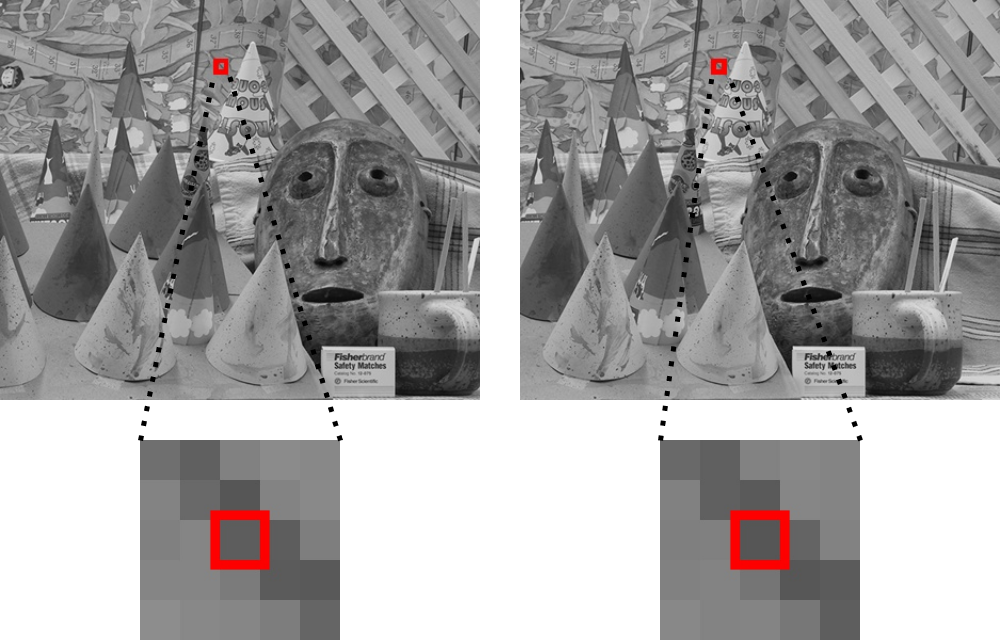
\includegraphics[width=0.8\linewidth]{Images/Chap_4/Cones.png}
  \caption{Homologous pixels in a pair of images. From \cite{malinowski_uncertainty_2024}}\label{fig:Cones}
\end{figure}

\begin{remark}
    Although the $\SAD$ is not the best performing cost function for dense matching, it is both fast and easily parallelizable. It is often use for comparison in cost-based stereo algorithms \cite{hirschmuller_evaluation_2007, zbontar_stereo_2016}, or in other applications. Considering a simple cost function such as $\SAD$ is relevant for different reasons:
    \begin{itemize}
        \item Simple stereo matching algorithms are often used as a quick and easy method for estimating the disparity.
        \item Simple cost functions (such as $\SAD$, ZNCC, \etc) considered here are still used in other problems, such as video compression for instance \cite{richardson_h264_2006}.
        \item As both stereo matching and uncertainty propagation can be complicated problems, considering a simple stereo algorithm allow\comloic{allows?} us to remain (relatively) simple and didactic in our explanations. \comloic{peut être qu'au lieu de te justifier par copie de ce que font les autres tu peux dire que tu te places dans un scénario favorable pour SAD en connaissant ses limitations (pas robuste à un gain et un offset entre les patchs, si tu travailles sur cones dans les mm conditions d'expo et d'illumination SAD c'est parfait, et tout le reste est superflu}
    \end{itemize}
\end{remark}

As stated previously, we will not consider in this chapter the use of Semi Global Matching (or similar regularization methods), as it necessitates many operations due to its recursive formulation and thus greatly increases complexity for the uncertainty propagation. We diverge from state-of-the-art methods to keep explanations as simple as possible, however the modeling of uncertainty for more advanced cost functions and \acrshort{sgm} methods will be considered in \Cref{chap:epistemic_uncertainty}.\comloic{on dirait que tu sens coupable un peu... à ce stade c'est au moins la troisième fois que tu le dis... peut être que tu peux le défendre une bonne fois pour toute en préambule}

\begin{figure}
    \centering
    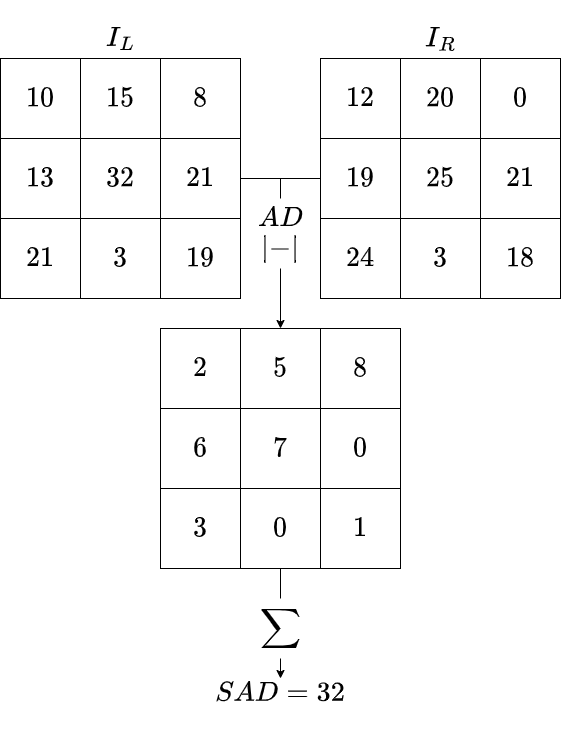
\includegraphics[width=0.5\linewidth]{Images/Chap_4/SAD.png}
    \caption{Diagram representing the $SAD$ cost function between two $3\times3$ patches. From \cite{malinowski_uncertainty_2024}}
    \label{fig:SAD}
\end{figure}

In our experiments, we considered the ``Cones'' images from the 2003 Middlebury stereo dataset (\url{https://vision.middlebury.edu/stereo/data/scenes2003/}), as presented in \Cref{fig:color_cones_image}. The two images have a of size $375 \times 450$, and the range of considered disparities is $[-60, 0]$.

\subsection{Uncertainty Model for Epipolar Images Intensities}
To maintain simplicity in this section, we will not consider panchromatic images, such as Pléiades products, encoding the reflectance values as positive integer, usually contained in $[0, 5000]$. Instead, we consider grayscale images that have intensity levels quantified within the range $[0, 255]$, which will represent our measurable space $\X$.

\begin{remark}
    This hypothesis is not constraining as we can easily normalize reflectances in order to encode them using 8-bit integers value, although doing so reduces the precision of the initial images. Moreover, this normalization step is often required to fit a given format, for instance if the images must be processed by a CNN trained on 8-bit integers.
\end{remark}

We hypothesize that a pixel's intensity value can deviate around its observed value with a range of $\pm i_\sigma$, with the observed value being the most likely. This specific hypothesis remains simple and relatively plausible with regards to the processing leading to the epipolar images. We then suppose that the uncertainty from the noise of the sensor capturing the image, from pre-processing steps such as atmospheric correction\commanue{alors cette étape je ne sais, après tu as tout de même des étapes de corrections radiométriques et géométriques} or epipolar resampling (see \Cref{sec:uncertainty_cars}) or from the quantification of observed radiometric values into integers\commanue{je ne suis pas sure de comprendre}, are not exactly known, but can be model by a possibility distribution\comloic{lien vers le chapitre 2 ?}. Consequently, we model the uncertainty of each pixel $p\in I_L,I_R$ intensity with a possibility distribution $\pi$, centered around the observed intensity $i_p\in[0,255]$:
\begin{equation}\label{eq:pixel_possibility}
    \pi(i_p)=1,\quad \pi(i_p\pm i_\sigma)=\alpha\,,
\end{equation}
with $\alpha \in [0,1]$. To remain simple, we chose $i_\sigma=1$ in the following, which is relatively narrow but allows simplification without impacting our reasoning. Similarly, we do not consider multiple $\alpha$ values in order to limit the number of focal sets considered. Choosing thus simple possibility distribution is convenient, but results obtained in this chapter can easily be extended to more complex possibility distributions. In our simulation, $\alpha = 0.3$ for pixels in the left image and $\alpha = 0.4$ for pixels in the right image\commanue{Je ne sais pas si tu synthétises les valeurs quelque part mais ce serait cool, ça peut être un tableau en annexe, sinon ça oblige à relire la section pour retrouver les valeurs}. We use different values of $\alpha$ for the left and right images because the uncertainty model may vary between images due to differences in exposure, noise levels, or camera calibration. The values on themselves are chosen arbitrarily for the purpose of this example. From a credal set interpretation\comloic{lien vers la définition ou rappel ici}, this model effectively states that we accept any probability distribution\comloic{lien également} supported within $[i_p - 1, i_p + 1]$ where the probability measure $P$ satisfies $\{P(A) \leq \sup_{i \in A} \pi(i)\}$ as an acceptable model for our uncertainty. The mass distribution\comloic{idem lien} function $m_p$ associated to this credal set possesses two focal sets\comloic{idem} $a^p$:
\begin{eqnarray}
    &m_p(a^p_1=\opi i_p, i_p\cli)=1-\alpha\,\nonumber\\
    &m_p(a^p_2=\opi i_p-1, i_p + 1\cli)=\alpha\,\label{eq:pixel_mass}
\end{eqnarray}
with $\opi\cdot, \cdot\cli$ referring to integer intervals. In particular, $\opi i_p, i_p\cli$ correspond to the singleton $\{i_p\}$.\comloic{je me demande à quel point ça vaudrait pas le coup de faire un tableau qui reprend les termes définis aux chapitres 2 et 3 et les traduis dans le cadre du chapitre 4. Si le lecteur découvre la plupart des définitions et notations exposées aux chapitres 2 et 3, alors ça va être dur pour lui de lire la version numérique de la thèse s'il n'y a pas un rappel voire une reformulation dans le cadre concret du chapitre 3.}

\begin{remark}
    The hypothesis of modelling the uncertainty on image intensities by possibility distributions does not consider uncertainty from potentially bigger sources of errors, such as satellite vibrations during the acquisition, or errors in the computations of epipolar lines. Those type of errors have been encountered on some Pléiades acquisitions, and lead to significant biases and errors on the final DSM, that our simple model does not account for. However, the CO3D mission will acquire images using a CCD matrix sensor rather than push-broom sensors used in Pléiades, so we can safely assume that those problems should not be encountered on images from the CO3D mission\commanue{Bon disons plutôt que la correction géométrique des images a pour objectifs de tenir compte de ces erreurs éventuelles et de les minimiser.}\comloic{mouais... on s'attend déjà à pas mal de vibrations, c'est pas lié au mode d'acquisition mais plutôt à la stabilité de l'ensemble de la plateforme, et de ce côté là CO3D c'est censé être Dacia pendant Pléiades c'est une voiture de luxe et sur mesure. Donc il y aura masse de vibrations. Pour ce qui est des lignes épipolaires, on peut faire des erreurs simplement au niveau des SiFT. Difficile d'argmenter à ce stade que les SiFTs seront plus robustes sur produits CO3D. Donc je dirai plutôt que tu fais l'hypothèse, pourquoi pas plausible, que les modèles géométriques sont parfaitement affinés et que la géométrie épipolaire estimée selon la méthode présentée chapitre 1 est également parfaitement estimée.}.
\end{remark}


\subsection{Dependency Model between Epipolar Images}
We presented the uncertainty models for pixels in both images, but we also need to define the dependency model between every pixel of both images. Indeed, as some pixels between images represent the light reflected by the same object, it seems natural that their (uncertain) values are correlated. In our case, we propose to model their dependency with the product copula if the pixels are not from the same physical object, meaning that the value of their intensities are independent. For pixels belonging to the same object, we model their dependency by a Gaussian copula with a covariance matrix $R$. Those copulas were presented in \cref{eq:gaussian_copula} from \Cref{chap:representation_of_uncertainty}. We remind here the formulation of a Gaussian $n$-copula $C_R$:
\begin{align}
    C_R(u_1 \enum u_n)=\Phi_R(\Phi^{-1}(u_1) \enum \Phi^{-1}(u_n))\label{eq:gaussian_copula}
\end{align} where $\Phi_R$ is the joint multivariate CDF of a Gaussian variable with correlation matrix $R$, and $\Phi^{-1}$ is the inverse CDF of a univariate Gaussian variable.

The correlation values inside the covariance matrix are based on a segmentation $S:(I_L\cup I_R)\rightarrow\opi1,K\cli$, $K\in\mathbb{N}$, of the images. This segmentation is the result of a \textit{k-means} clustering performed on the ground truth disparity map. Example of such a clustering is presented in \Cref{fig:clustering_example}, with $K=8$. Given the segmentation $S$ and two pixels $(p, q)\in(I_L\cup I_R)^2$, their covariance is determined by
\begin{equation}\label{eq:correlation}
    \sigma(p, q) =
    \begin{cases}
        1 &\text{ if }p=q,\\
        \rho_k, &\text{ if } p\ne q\text{ and }S(p)=S(q)\,, \\
        0 & \text{otherwise}\,.
    \end{cases}
\end{equation}
where $0<\rho_k<1$ is the correlation of pixels belong to segment $k\in\opi 1, N\cli$. Given a set of pixels $\{p_1 \enum p_n\}\subseteq(I_L\cup I_R)^2$, their covariance matrix $R$ is therefore:
\begin{align}
    R = \begin{bmatrix}
        1 & \sigma(p_{1}, p_{2}) & \dots & \sigma(p_{1}, p_{n-1}) & \sigma(p_{1}, p_{n})\\
        \sigma(p_{2}, p_{1}) & 1 & \dots & \sigma(p_{2}, p_{n-1}) & \sigma(p_{2}, p_{n})\\
        \dots & \dots & \dots & \dots & \dots\\
        \sigma(p_{n-1}, p_{1}) & \sigma(p_{n-1}, p_{2}) & \dots & 1 & \sigma(p_{n-1}, p_{n})\\
        \sigma(p_{n}, p_{1}) & \sigma(p_{n}, p_{2}) & \dots & \sigma(p_{n}, p_{n-1}) & 1
    \end{bmatrix}
\end{align}

In practice, we will only compute the correlation matrix between the two windows from the reference and secondary images that are compared. The\comloic{Both windows? comme ça on fait encore mieux le lien entre Guassian 18 et le paramétrage} windows have a $3\times 3$ shape, we thus consider Gaussian $18-$copulas to model the dependency between pixels. This copula will be used for joining marginal masses in the uncertainty propagation step using \cref{eq:joint_mass} from the previous chapter. It will also be used to sample for Monte Carlo sampling, used for evaluating the correct uncertainty propagation in \Cref{sec:montecarlo}\commanue{Il y a beaucoup de used dans les phrases, je trouve que cette pĥrase complique les choses. Peut-être juste mentionner qu'on utilise la copule gaussienne quand on arrive à ces sujets}.

\begin{remark}\commanue{remarque globale avec les encarts remark, fais attention à ne pas en abuser car on a tendance à perdre le fil. Cette remarque tu pourrais la mettre au début de la section quand tu dis que tu choisis des copules gaussiennes.}\comloic{oui ou même à la fin pour ne pas faire flipper dès le début. Cest clair que si on pouvait lire déjà la version limpide et fluide avant d'avoir toutes les remarques ce serait pas mal. Là on dirait que c'est écrit comme si tu avais peur qu'on arrête de lire à chaque instant en se disant "oh la la il passe carrément ce truc qui s'applique pas à son cas sous silence c'est inadmissible". Vu que la plupart du temps c'est pour dire que ça s'applique pas d'une façon ou d'une autre, autant laisser la lecture se fluidifier et le lecteur prendre confiance avant de lui dire "bon, mnt que t'as compris l'idée, voici les limitations, les autres façon de faire, d'autres trucs que tu pourrais lire ou avoir lu dans la litérrature et qui ne s'appliquent pas ici d'après moi}
    Gaussian copulas are popular and simple copulas used to represent dependencies between more than $2$ variables. By comparison, the different $2$-copulas presented in \Cref{sec:copulas} cannot always be defined in more than $2$ dimensions or possess a quite complex formulation. Another method for modelling the dependency for more than $2$ variables is to express a $n$-copula as a combination of $2$-copulas, which is called a vine copula (\cite{czado_vine_2022}). However this is a complex subject that is not adapted to our type of dependency, and is therefore not explored in this thesis.
\end{remark}

\begin{figure}
    \centering
    \begin{subfigure}[t]{0.5\linewidth}
        \centering
        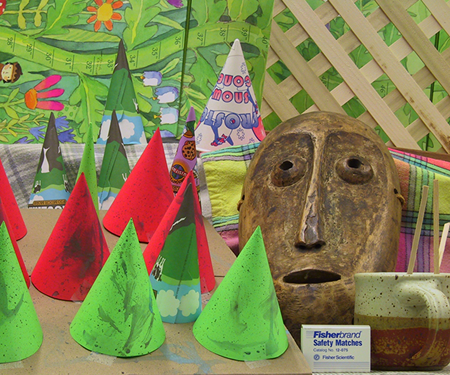
\includegraphics[width=0.9\linewidth]{Images/Chap_4/im2.png}
        \caption{Colored left image}
        \label{fig:color_cones_image}
    \end{subfigure}\hfill
    \begin{subfigure}[t]{0.5\linewidth}
        \centering
        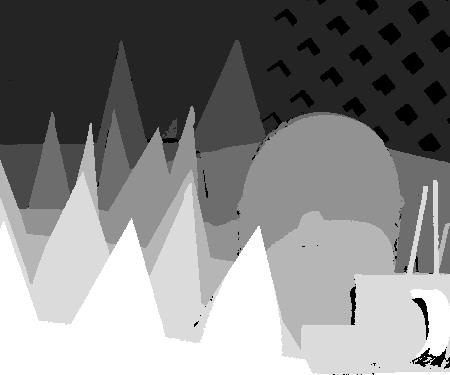
\includegraphics[width=0.9\linewidth]{Images/Chap_4/cluster.jpg}
        \caption{Proposed clustering of the image (\textit{k-means} with $K=8$)}
        \label{fig:cluster}
    \end{subfigure}
    \caption{Middlebury 2003 Cones left image, and a clustering computed from the disparity ground truth.}
    \label{fig:clustering_example}
\end{figure}

During our simulations, the segmentation contains $K=8$ different clusters. For every $k$ in $\opi1,K\cli$, $\rho_k$ is assigned an value between $0.9$ and $1$ in order to really emphasize on their correlation.\commanue{à mon avis tu peux regrouper cette phrase dans le milieu paragraphe précédent où tu décris ton modèle. Là elle se retrouve un peu isolée}

\begin{remark}\comloic{plus haut tu fais une remarque sur le fait que tu ne considères par les incertitudes sur les modèles géo et la mise en géo épipolaire. Ici ne faut il pas parler des incertitudes sur la segmentation que tu fais ? De quelle façon est ce qu'elle impacte les conclusions ? Ca vaut le coup de rappeler que la VT est obtenue par construction car tu travailles sur les cones, peut être rappeler les conditions d'acquisitions des images. L'idée sous jacente étant de dire que dans un cadre lambda, la VT n'est pas une VT parfaite, la segmentation de la VT ne l'est pas non plus et même si elle l'était, la VT étant imparfaite on pourrait avoir des incohérences avec les images qui elles mêmes peuvent ne pas avoir été acquises de façon synchrones. En gros tu parles un peu de Pléiades de et CO3D donc on a parfois l'impression que ce que tu vas présenter pourrait s'adapter à ce type de données. Faut peut être préciser en quoi tes expérimentations s'éloignent un peu de tout ça.}
    The segmentation is based on the ground truth disparity map. This means that two objects with similar disparities located at opposite sides of the image will be considered as belonging to the same object and thus correlated. In practice, those pixels are never compared as we only measure the dissimilarity between small windows in a restricted disparity range. The clustering is thus only used at a \textit{local} scale. 
    
    Secondly, the segmentation allows to compute the Gaussian copula, which will be used to propagate the uncertainty models. We will validate the uncertainty propagation in \Cref{sec:montecarlo} with Monte Carlo samples using the same copula. As long as the copulas used are the same between the propagation and validation, it does not really matter which correlation matrix is used. We still tried to create a realistic but simple dependency model for the sake of the example, but it is not required from a theoretical point of view\commanue{là trop de remarques tue la remarques. Tu n'es pas obligé de faire des teasers sur tous les points que tu vas abordés. Je me limiterais à donner les infos qui correspondent au modèle de dépendence entre les images qui est le thème de la section. Si par la suite tu as besoin de réutiliser les copules, bah tu le dis.}.
\end{remark}

\section{Propagating the Uncertainty with Belief Functions and a Copula}
Having defined both marginal models for pixel intensities using possibility distributions as well as\comloic{and c'était aussi bien en fait vu que tu utilises pas la même chose pour définir les deux choses "marginals models" et "dependency models"} dependency models using copulas, we can now join them all to construct a multivariate uncertainty model, as seen in \Cref{sec:methods_for_joining_credal_sets}. We will see in this section how the multivariate models can then be used to compute the uncertainty regarding the cost curve. 

\subsection{From Multivariate Uncertainty Models to the Propagated Model}
We first detail how multivariate models are used to propagate uncertainty in the precise case. We will then do the same in the imprecise setting by analogy.

Consider a mapping $f:\X_1\times\X_2\rightarrow\mathcal{Z}$ from a product space $\X_1\times\X_2$ to a space $\mathcal{Z}$, which propagates multiple random variables $X_1$, $X_2$ to a new random variable $Z=f(X_1, ~X_2)$. In our case, $f$ will be the $\SAD$ cost function propagating the intensities to the matching cost. When considering precise probabilities, the probability of $Z$ on atoms $z$ is obtained by summing the probabilities of all events $X_1=x_1$, $X_2=x_2$ whose image by $f$ is $z$: 
\begin{align}\label{eq:precise_propagate_proba}
    \forall z\in\mathcal{Z}, P_Z(z)=\sum_{\substack{x_1,x_2\\z=f(x_1,x_2)}}P(x_1,x_2).
\end{align}
where $P(x_1,x_2)$ is the joint probability, which is linked to its marginals by a copula $C$. $P_Z$ is completely determined by evaluated\comloic{evaluating, il y en a quelques autres dans le texte, j'en ai corrigé certains en live je laisse ici en commentaire car je suis pas sur de tous les avoir vu} every combination of atoms of $\X_1$ and $\X_2$.

\begin{example}\label{ex:propagated_probability}
    Consider the same setting as example \ref{ex:copulas}, where a dealer throws two coins in a separate room. The coins seem fair when looked at independently. In this example, a coin landing on heads rewards you with $1$€ (or any currency of your choice), and a coin landing on tails rewards you with $0$€. So you earn $2$€ if both coins land on heads, $1$€ if only one coin land on heads, and $0$€ if both coins land on tails. We are interesting in the uncertainty regarding you earnings, noted $Z$.
    
    In example \ref{ex:copulas}, we consider $3$ different cases, each leading to a different copula $C$ modelling the dependency between the probability $P_1$ of first coin and $P_2$ of the second coin. For each copula, we then computed the joint probability $P$.
    
    In the first case, where coin throws were independent, we saw that the joint probability $P$ was:\\
    \begin{minipage}[b]{0.5\linewidth}
    \begin{align*}
        & P(\text{heads}, ~\text{heads}) = 0.25\\
        & P(\text{heads}, ~\text{tails}) = 0.25
    \end{align*}
    \end{minipage}
    \begin{minipage}[b]{0.5\linewidth}
    \begin{align*}
        & P(\text{tails}, ~\text{tails}) = 0.25 \\
        & P(\text{tails}, ~\text{heads}) = 0.25
    \end{align*}
    \end{minipage}
    In that case, it holds that the probability $P_Z$ of our earnings are:
    \begin{align*}
        & P_Z(Z=2) = P(\text{heads}, ~\text{heads}) = 0.25\\
        & P_Z(Z=1) = P(\text{heads}, ~\text{tails}) + P(\text{tails}, ~\text{heads}) = 0.5 \\
        & P_Z(Z=0) = P(\text{tails}, ~\text{tails}) = 0.25
    \end{align*}
    
    In the second case, where coin throws were rigged to land on the same side, we saw that the joint probability $P$ was:\\
    \noindent
    \begin{minipage}[b]{0.5\linewidth}
    \begin{align*}
        & P(\text{heads}, ~\text{heads}) = 0.5\\
        & P(\text{heads}, ~\text{tails}) = 0
    \end{align*}
    \end{minipage}
    \begin{minipage}[b]{0.5\linewidth}
    \begin{align*}
        & P(\text{tails}, ~\text{tails}) = 0.5\\
        & P(\text{tails}, ~\text{heads}) = 0 
    \end{align*}
    \end{minipage}
    Following the same methodology, we have:\\
    \noindent\begin{minipage}[b]{0.33\linewidth}
    \begin{align*}
        & P_Z(Z=2) = 0.5
    \end{align*}
    \end{minipage}
    \begin{minipage}[b]{0.33\linewidth}
    \begin{align*}
        & P_Z(Z=1) = 0
    \end{align*}
    \end{minipage}
    \begin{minipage}[b]{0.33\linewidth}
    \begin{align*}
        & P_Z(Z=0) = 0.5
    \end{align*}
    \end{minipage}
    
    In the third case, where coin throws were rigged to land on opposite sides, we saw that the joint probability $P$ was:\\
    \noindent\begin{minipage}[b]{0.5\linewidth}
    \begin{align*}
        & P(\text{heads}, ~\text{heads}) = 0\\
        & P(\text{heads}, ~\text{tails}) = 0.5
    \end{align*}
    \end{minipage}
    \begin{minipage}[b]{0.5\linewidth}
    \begin{align*}
        & P(\text{tails}, ~\text{tails}) = 0\\
        & P(\text{tails}, ~\text{heads}) = 0.5
    \end{align*}
    \end{minipage}
    Therefore:\\
    \begin{minipage}[b]{0.33\linewidth}
    \begin{align*}
        & P_Z(Z=2) = 0
    \end{align*}
    \end{minipage}
    \begin{minipage}[b]{0.33\linewidth}
    \begin{align*}
        & P_Z(Z=1) = 1
    \end{align*}
    \end{minipage}
    \begin{minipage}[b]{0.33\linewidth}
    \begin{align*}
        & P_Z(Z=0) = 0
    \end{align*}
    \end{minipage}
\end{example}

Determining every $(x_1, x_2)$, whose image by $f$ equals $z$, is not always trivial. This becomes even more complex when considering $n>2$ marginal variables. Similarly, the joint probability $P(x_1,x_2)$ is computed using a H-volume, which is the sum of $2^n$ terms, thus also increasing exponentially with the dimension.

There are multiple ways of extending \cref{eq:precise_propagate_proba} to the imprecise setting, as there are multiple ways of aggregating imprecise models using a copula. We presented\commanue{tu emploies bcp cette formule, donc de temps en temps described/} in \Cref{chap:joining_credal_sets} three methods for joining marginal credal sets, creating three different multivariate credal sets $\M_{robust}$, $\M_{mass}$ and $\M_{agg}$.

The robust approach of extending \cref{eq:precise_propagate_proba} is based on the robust approach from \Cref{sec:robust_method}. Given $n$ marginal credal sets $\M_i$, we can join them using a copula $C$ into a credal set $\M_{robust}$ as in \eqref{eq:robust_set}. The propagated uncertain model $\M^Z_{robust}$ is then defined as:
\begin{align}
    \M^Z_{robust} = \{P_Z~|~\forall z\in Z, ~P_Z(z)=\sum_{\substack{x_1 \enum x_n\\z=f(x_1 \enum x_n)}}P(x_1 \enum x_n), ~P\in\M_{robust}\}
\end{align}
Practically, this set is computed by sampling every probability $P_i$ from each marginal credal set $\M_i$ and joining them using \hyperref[theorem:sklar]{Sklar's Theorem} into a multivariate probability $P$\comloic{typiquement là ça vaut le coup de traduire en stereo matching par SAD, je tiens des notes mais sans ça c'est pas évident de se raccrocher. Si je note pas un truc je suis obligé de repartir dans le chapitre 2, ou 3, ou 4.1 pour retracer les liens. Après c'est peut être limpide pour ton jury ceci dit}. Then for each $z=P(x_1 \enum x_n)$, we can compute $P_Z$ from $P$ using \eqref{eq:precise_propagate_proba}. In short, each sample $(P_1 \enum P_n)$ leads to a new $P$, itself leading to a new $P_Z$. Sampling through every $(P_1 \enum P_n)$ thus leads to the estimation of the uncertain model of $Z$. This method is complicated to compute, but correctly propagates the uncertainty.

We saw that it was easier to compute $\M_{mass}$ than $\M_{robust}$. Another way\commanue{mot de liaison entre les deux phrase. So another way or Thus another way} of approximating the uncertainty model of $Z$ is to compute it using $\M_{mass}$. This is done by replacing the probability on atoms from \cref{eq:precise_propagate_proba} with the joint mass $m_\times$ from \cref{eq:joint_mass} \cite{gray_dependent_2021}. Consider $n$ uncertain variables $X_i$, each modeled by a mass distribution function whose $j$-th focal set is noted $a^i_j$. Given their multivariate mass $m_\times$, it is possible to compute the mass distribution function $m_Z$ of a random set $Z=f(X_1 \enum X_n)$ as:
\begin{align}
    \forall a^Z\subseteq\mathcal{Z}, m_Z(a^Z) = \sum_{\substack{a^1_i \enum a^n_j\\a^Z=f(a^1_i \enum  a^n_j)}}m_\times(a^1_i \enum a^n_j)\label{eq:mass_propagated}
\end{align}
leading to a credal set $\M_{mass}^Z$:
\begin{align}
    \M_{mass}^Z &= \{~P_Z~|~\forall A\subseteq\mathcal{Z},~P_Z(A)\geqslant \sum_{a^Z\subseteq A}m_Z(a^Z)\}\\
    &=\{~P_Z~|~\forall A\subseteq\mathcal{Z},~P_Z(A)\geqslant \sum_{\substack{a^1\enum a^n \\ f(a_1\enum a_n)\subseteq A}}m_\times(a^1\enum a^n)~\}
\end{align}

In order to compute the propagated mass $m_Z$ (and its associated belief function) from \cref{eq:mass_propagated}, two difficulties arise. The first one is to determine what the focal sets $a_Z$ of $m_Z$ will be, which corresponds to the subscript $a^Z=f(a^n_1 \enum  a^n_j)$ of the previous sum. Computing the image of $f$ for every combination of focal sets $(a^1_i \enum a^n_j)$ is even more difficult than in the precise case, as we are computing images of sets instead of real numbers. The second difficulty is to compute the joint mass $m_\times$, as in the case of the $\SAD$ it requires to compute the H-volume of an $18$-copula. Those difficulties will be addressed in the following sections \ref{sec:propagated_focal_sets} and \ref{sec:propagated_masses}

We saw in \Cref{chap:joining_credal_sets} that in the situation where marginals are possibility distributions, $\M_{mass}$ and $\M_{agg}$ have the same bounds on Cartesian products of events (see \cref{eq:inclusion_necessity}). We will thus only compute the lower bounds $Bel_\times$ of $\M_{mass}$ as it directly provides the bounds of $\M_{agg}$ on those events\commanue{tu n'as pas inversé $\M_{mass}$  et $\M_{agg}$ dans ta phrase ? $\M_{agg}$ c'ets pas celui qui est plus facile à calculer}.

\subsection{Determining the Propagated Focal Sets}\label{sec:propagated_focal_sets}
In this section, we will detail how we compute the $\SAD$ image of marginal focal sets. Computing the image of sets needs to be treated with caution in the general case. However in our case, because we chose marginal focal sets with a simple expression, and because we are using a relatively regular cost function, computing the image is significantly easier.

Given a pixel $p$, we consider the mass distribution $m_p$ of \cref{eq:pixel_mass} and its two focal sets $a_1^p$ and $a_2^p$ from \cref{eq:pixel_mass}. For every pair of pixels $p\in I_L, q\in I_R$, we note $\AD_{pq}=|i_p - i_q|$, where $i$ refers to a pixel's intensity. Given $m_p$, There\comloic{there avec un t miniscule non?} exist $3$ focal sets related to the absolute difference:
\begin{itemize}
    \item $a^{\AD}_1$ is the image of the AD of $a^p_1$ and $a^q_1$
    \item $a^{\AD}_2$ is the image of the AD of $a^p_2$ and $a^q_1$ or $a^p_1$ and $a^q_2$
    \item  $a^{\AD}_3$ is the image of the AD of $a^p_2$ and $a^q_2$
\end{itemize}
The non-monotonicity of the absolute value around $0$ needs to be taken into account to compute their exact image through the AD. Indeed, if a value $x$ is in $[-1,1]$, then its absolute value will be in $[0,1]$. Applying this remark to the AD yields the following focal sets:
\begin{align*}
    a^{\AD}_1&=\opi\AD_{pq},~\AD_{pq}\cli\,,\\
    a^{\AD}_2&=\opi\max(0, \AD_{pq} - 1),~\AD_{pq} + 1\cli\,,\\
    a^{\AD}_3&=\opi\max(0, \AD_{pq} - 2),~\AD_{pq} + 2\cli\,,
\end{align*}

Focal sets of the final $\SAD$ are then computed by simply summing the bounds of the $9$ AD focal sets\comloic{j'ai raté un truc, tu dis deux fois plus haut, il me semble, qu'on a 3 AD focal sets pour un ADpq (pour une mesure AD pixel à pixel entre p et q) selon que pour p, et/ou q, on soit sur la radiométrie inscrite dans les images ou bien que l'on soit en réalité sur une radiométrie dans un voisinage e sigma=1 autour de celle inscrite dans les images? Comment ça fait 9 AD focal sets et pas 81 pour une SAD sur des fenêtres 3x3 ? J'ai du me louper quelque part...} (as in \Cref{fig:SAD}), for every combination $(a^{\AD_1}_{k_1}\enum a^{\AD_9}_{k_9})$ of those focal sets\comloic{$(\AD_9)$ c'est AD entre p=9 et q=9 ? et k9 ça correspond à quel focal set pour AD9 ? Le premier le deuxième ou le troisième ? Ou un résumé des trois genre les deux bornes les plus, respectivement, petites et grandes parmi les 3 focal set de $(AD_99)$ ?}:
\begin{align}
    a^\SAD=\sum_{i=1}^9a^{\AD_i}_{k_i}
\end{align}

\begin{remark}\comloic{alors 2 remarques sur ta remarque ^^' 1) pourquoi c'est une remarque ? On dirait que tu peux commencer par "En pratique", ou tout simplement "In many cases". On ne sait plus trop comment aborder les remarques sinon car il n'y a pas vraiment de tendances. Parfois c'est une façon d'annoncer que tu laisses consciemment un truc de côté car tu le juges non applicables. Parfois c'est pour dire qu'on pourrait aller plus loin mais que ça vaut pas la peine. Parfois c'est pour dire que d'autres utilisent d'autres modélisation mais qu'on n'a pas fait ce choix dans la thèse. Et là c'est juste la continuité je trouve. Donc selon le temps qu'il te reste ça pourrait valoir le coup de faire une passe sur les remarques, ça ne simplifie pas forcément la lecture au final, et ça donne l'impression que c'est pas net, et que ce sont des notes pour toi mêmes parfois, ou disons des choses qui te sont passées par là au moment où tu écrivais le reste et pour ne pas oublier tu as fait une remarque comme on prend une note. 2) C'est pas évident évident les notations et les termes ici. Je comprends l'histoire des 3 ai qui en pratique sont "symmétrique" si AD > 2*sigma, mais c'est pas fluide dans les définitions de AD, des AD focal sets, des aiAD, des ak etc. Ou bien c'est moi aussi peut être. Je te laisse voir si tu as une meilleure idée en seconde passe mais j'avoue que ce serait au risque de créer des boulettes}
    In many cases, different combinations of $\AD$ focal sets will lead to the same $\SAD$ focal set. Actually, if every $\AD$ is greater than $2$\commanue{alors je ne suis pas sure de comprendre} (so that each $a^\AD_i$ is symmetric with regards to its $\AD$) there will only be $19$ focal sets $a^\SAD$ for the $\SAD$, and they are of the following form:
    \begin{align}\label{eq:nested_SAD}
        a^\SAD = \opi\SAD-t,\SAD+t\cli,\text{ with }t\in\opi0, ~18\cli
    \end{align}
    In comparison, there are $3^9=19683$ different combinations of $\AD$ focal sets.
\end{remark}

\begin{remark}\commanue{pourquoi tu mets ce qui concerne SAD dans des remarques ?}
    In the previous remark, we established that when every $\AD$ is greater than $2$, it holds that:
    \begin{align*}
        a^\SAD = \opi\SAD-t,\SAD+t\cli,\text{ with }t\in\opi0, ~18\cli
    \end{align*}
    This equation translates the fact that focal sets of the $\SAD$ form an increasing family of events. This also means that $\Bel_\SAD$ is actually a necessity function\comloic{peut être rajouter des liens, j'ai tendance à devoir revenir aux définitions si j'ai pas mes notes à côté de mon PC et j'ai tendance à lire la thèse depuis différents endroits pour rester concentré}. We can thus compute a possibility distribution $\pi_\SAD$ to represent the uncertainty of the $\SAD$. This can be useful for graphically representing the uncertainty of the $\SAD$, if we later need to build joint uncertainty models using the $\SAD$, or if we want to propagate the $\SAD$ uncertainty even further.
    
    We proved in \cite{malinowski_uncertainty_2024} that in order to propagate marginal possibility distributions $\pi_i$ into a possibility distribution $\pi_Z$ using a copula and a propagating function $f$, a sufficient condition was that\commanue{tu n'as pas deux conditions dans ce qui suit}:
    \begin{itemize}
        \item $f$ is a monotone function applied to a linear combination $\alpha_1X_1+\dots+\alpha_nX_n+\beta$ of marginal variables $X_i$
        \item Each $\pi_i$ is symmetrical and uni-modal (meaning that all values $x_i$ such that $\pi_i(x_i)=1$ are adjacent). For instance all triangular possibility distributions verify this condition
    \end{itemize}
    Here is an example of an uni-modal symmetrical possibility
    \centering{\begin{tikzpicture}[scale=1]
        \begin{axis}[%
          xlabel=$x$,
          ylabel=$\pi(x)$,
          xmin=2, xmax=8,
          ymin=-0.05, ymax=0.55,
          ytick={0, 0.15, 0.4, 0.5},
          yticklabels={$0$, $0.3$, $0.8$, $1$},
          scale only axis,
          width=7cm, height=3.5cm,
          ],
          \node (a) at (2, 0) {$\times$};
          \node (b) at (2.5, 0) {$\times$};
          \node (c) at (3, 0) {$\times$};
          \node (d) at (3.5, 0.15) {$\times$};
          \node (e) at (4, 0.4) {$\times$};
          \node (f) at (4.5, 0.5) {$\times$};
          \node (g) at (5, 0.5) {$\times$};
          \node (h) at (5.5, 0.5) {$\times$};
          \node (i) at (6, 0.4) {$\times$};
          \node (j) at (6.5, 0.15) {$\times$};
          \node (k) at (7, 0) {$\times$};
          \node (l) at (7.5, 0) {$\times$};
          \node (m) at (8, 0) {$\times$};
          
          \draw [thick, dashed, gray] (a.center) -- (b.center) -- (c.center) -- (d.center) -- (e.center) -- (f.center) -- (g.center) -- (h.center) -- (i.center) -- (j.center) -- (k.center) -- (l.center) -- (m.center) ;
          \draw [decorate,decoration={brace,amplitude=5pt,mirror,raise=1ex},gray] (f.south) -- (h.south) node[midway,yshift=-2em]{\color{gray}{mode}};
        \end{axis}
    \end{tikzpicture}}
\end{remark}

\subsection{Computing the Mass of Propagated Focal Sets}\label{sec:propagated_masses}
%\section{Leveraging Specificities to Accelerate Computations}
Now that the bounds of the $\SAD$ have been computed\commanue{alors moi j'ai compris qu'on avait calculé les focal sets. J'ai pas bien vu le calcul des bornes}, we need to compute the associated mass. Computing the joint mass over two $3 \times 3$ windows is significantly more complex. For each combination of marginal focal sets, the joint mass $m_{\times}$ is computed using the H-volume of an $18$-copula, involving a sum of $2^{18}$ terms. Given that the uncertainty of each of the 18 pixels is represented by $2$ focal sets, we need to evaluate $2^{18}$ combinations of these focal sets in total\commanue{c'est juste moi qui comprends pas la subtilité }. This computation can thus become quite costly in memory and computation time, especially when computing it over a whole image.

In the case of the family of Gaussian copulas, their expression given by \cref{eq:gaussian_copula} show that we need to compute the multivariate CDF. An $18$-variate Gaussian CDF does not possess a known analytic formula, it is thus computed by integrating its density (so integrating a $18$-variate function), as expressed below:
\begin{align}\label{eq:gaussian_cdf}
    F(x_1 &\enum x_{18}) =\nonumber\\ &\int_{-\infty}^{x_1}\dots\int_{-\infty}^{x_{18}}\frac{1}{\sqrt{(2\pi)^{18}|R|}}\exp(-\frac{1}{2}\begin{bmatrix}x_1 & \dots & x_{18}\end{bmatrix}R^{-1}\begin{bmatrix}x_1 \\ \dots \\ x_{18}\end{bmatrix})dx_1\dots dx_{18}
\end{align}
Where $|R|$ is the determinant of $R$. Computing this CDF can quickly become time-consuming ($40ms$ on average\footnote{With an AMD EPYC7713  64-Core Processor at 2GHz, using Python and the SciPy library}). For each pixel and each disparity, we saw that we need to compute the joint mass of $2^{18}$ focal sets, each time necessitating $2^{18}$ evaluation of its copula. Because there are around $170\,000$ pixels and $60$ disparities to be evaluated, the processing time is too large to be computed as such. We will instead see that we can leverage specificities of our problem to drastically reduce the computation time.
 
The first idea is to notice than if we can divide our variables into multiple mutually independent sets of variables, then the evaluation of the $18$-copula can be separated into the evaluation of multiple lower dimension copulas. To verify this statement consider the following independent sets of variables $\{X_1 \enum X_k\}$ and $\{X_{k+1} \enum X_n\}$ with $k\in\opi1,n-1\cli$. Let $F_1 \enum  F_n$ be their marginals CDF. And let $F_{(1 \enum n)}$ be the joint CDF of all variables, $F_{(1 \enum k)}$ the joint CDF of the first set of variables and $F_{(k+1 \enum n)}$ the joint CDF of the second set. The two sets are independent means\comloic{peut être mettre des guillemets autour de "The two sets are independant" du coup ?} that for all $(x_1 \enum x_n)\in\X_1\tdt\X_n$ it holds that:
\begin{align*}
    F_{(1 \enum n)}(x_1 \enum x_n) = F_{(1 \enum k)}(x_1 \enum x_k)\cdot F_{k+1 \enum n}(x_{k+1} \enum x_n)
\end{align*}
Using Sklar's theorem, there exist a $n$-copula $C$, a $k$-copula $C'$ and a $n-k$-copula $C''$ respectively linking $F_{(1 \enum n)}$, $F_{(1 \enum k)}$, and $F_{(k+1 \enum n)}$ to their marginals:
\begin{align}
    C(F_1(x_1) \enum F_n(x_n)) = C'(F_1(x_1) \enum F_k(x_k))\cdot C''(F_{k+1}(x_{k+1}) \enum F_n(x_n))\label{eq:copula_factorizing}
\end{align}

\begin{remark}
    We stated earlier that we did not considered vine copulas \cite{czado_vine_2022}, which are a way of constructing multivariate copulas by composition of bivariate (conditional) copulas. The decomposition $C$ into $C'$ and $C''$ actually follows the same idea of decomposing a copula into smaller ones. So even though we are not using vine copulas, we use a similar philosophy in our computations.
\end{remark}

Establishing \cref{eq:copula_factorizing} becomes interesting once we put it in relation with the following property:
\begin{proposition}[H-Volume factorizing]\label{prop:hvol_factorizing}
    Let $1<k<n$. If a $n$-copula $C$ can be expressed as the product of a $k$-copula $C'$ and a $(n-k)$-copula $C''$, then the H-volume of $C$ is the product of the H-volume $H'$ of $C'$ and the H-volume $H''$ of $C''$. This means that for all $(u_1 \enum u_n)\in[0,1]^n$ and for all $(v_1 \enum v_n)\in[0,1]^n$ such that $u_i\leqslant v_i$, it holds that:
    \begin{align}
        H_{u_1 \enum u_n}^{v_1 \enum v_n} = {H'}_{u_1 \enum u_k}^{v_1 \enum v_k}\cdot{H''}_{u_{k+1} \enum u_n}^{v_{k+1} \enum v_n}
    \end{align}
\end{proposition}
\begin{proof}
    Let $1<k<n$, $C$ a $n$-copula, $C'$ a $k$-copula and $C''$ a $n-k$ copula. $H$, $H'$, $H''$ are the respective H-volume of $C$, $C'$, $C''$. then
    \begin{align*}
        %{H'}_{u_1 \enum  u_k}^{v_1 \enum  v_k}\times {H''}&_{u_{k+1} \enum  u_n}^{v_{k+1} \enum  v_n} = \left(\sum_{w_i\in\Pi_{i=1}^{k}\{u_i,v_i\}}(-1)^{|\{w_i~|~w_i=u_i\}|}C'(w_1 \enum w_k)\right)\\
        {H'}
        \begin{matrix}
            v_1 \enum  v_k\\
            u_1 \enum  u_k
        \end{matrix}
        \cdot {H''}&
        \begin{matrix}
            v_{k+1} \enum  v_n\\
            u_{k+1} \enum  u_n
        \end{matrix}= \left(\sum_{w_i\in\Pi_{i=1}^{k}\{u_i,v_i\}}(-1)^{|\{w_i~|~w_i=u_i\}|}C'(w_1 \enum w_k)\right)\\
        &\times\left(\sum_{w_j\in\Pi_{j=k+1}^{n}\{u_j,v_j\}}(-1)^{|\{w_j~|~w_j=u_j\}|}C''(w_{k+1} \enum w_n)\right)\\
        =& \sum_{w_i\in\Pi_{i=1}^{k}\{u_i,v_i\}}\times\sum_{w_j\in\Pi_{j=k+1}^{n}\{u_j,v_j\}}(-1)^{|\{w_i~|~w_i=u_i,~i\leqslant k\}|}\\
        &\times(-1)^{|\{w_j~|~w_j=u_j,~ j>k\}|}C'(w_1 \enum w_k)C''(w_{k+1} \enum w_n)\\
        =&\sum_{w_i\in\Pi_{i=1}^{n}\{u_i,v_i\}}(-1)^{|\{w_i~|~w_i=u_i\}|}C'(w_1 \enum w_k)\\
        &\times C''(w_{k+1} \enum w_n)\\
        =&H
        \begin{matrix}
            v_1 \enum  v_n\\
            u_1 \enum  u_n
        \end{matrix}
        %=&H_{u_1 \enum  u_n}^{v_1 \enum  v_n}
    \end{align*}
\end{proof}
Using the result of proposition \ref{prop:hvol_factorizing}, we can now compute the joint mass as a product of two lower dimension copulas. It is easier to compute as we only integrate a $k$-dimensional function and a $n-k$-dimensional function, instead of a $n$-dimensional one. Similarly the $H$ volume is not the sum of $2^{18}$ terms anymore, but the sum of $2^{k}$ and $2^{n-k}$ terms.

For comparison, consider that we can split the aforementioned Gaussian $18$-copula into two Gaussian $9$-copula. Computing the value of single mass used to take around $10\,500s$, but now takes around $6s$, so around $1\,700$ times faster. This demonstrates the substantial time savings achieved by decomposing the problem into smaller, independent parts. This improvements apply directly to our application. Indeed \cref{eq:correlation} yields the following correlation between two pixels $p$, $q$ given the segmentation $S$:
\begin{equation*}
    \sigma(p, q) =
    \begin{cases}
        1 &\text{ if }p=q,\\
        \rho_k, &\text{ if } p\ne q\text{ and }S(p)=S(q)\,, \\
        0 & \text{otherwise}\,.
    \end{cases}
\end{equation*}
From this, we can split the set $\{p_1 \enum p_{18}\}$ of pixels in at most $K=8$ mutually independent sets $S_k = \{p_i~|~S(p_i)=k\}$, each set containing pixels from the same cluster. We can thus compute the H-volume of each cluster independently.

Another additional way of reducing the computation time is to avoid computing the same $H$-volume multiple times. Consider a set $S_k$ with $k_L$ pixels from the left image and $k_R$ pixels from the right image. The correlation matrix $R_k$ for this cluster is:
\begin{equation}
    R_k=\begin{pmatrix}
        1 &  & \rho_k & \dots & \rho_k\\
         & & & & \vdots\\
        \rho_k &  & 1 & & \rho_k\\
        \vdots &  &  & & \\
        \rho_k & \dots & \rho_k &  & 1
    \end{pmatrix}\label{eq:corr_matrix_sym}
\end{equation}
which implies that the Gaussian $(k_L+k_R)$-copula for this set is symmetrical. The joint mass $m^{S_k}_\times$ of this set is then also symmetrical. Pixels from the left image will share the same mass $m_L$ for their two focal sets and pixel from the right image will also share the same mass $m_R$, therefore computing $m^{S_k}_\times$ on every possible combination of cumulative masses is redundant. 
\begin{example}
    Let us imagine a set $S_k$ with $k_L=2$ pixels $p_1$, $p_2$ from the left image and $k_R=2$ pixels $p_3$, $p_4$ from the right image. Each pixel $p_i$ has two focal sets $a^i_1$ and $a^i_2$.
    We know that:
    \begin{align*}
        m_L(a_1^1) &= m_L(a_1^2) \qquad m_L(a_2^1) = m_L(a_2^2)\\
        m_R(a_1^3) &= m_R(a_1^4) \qquad m_R(a_2^3) = m_R(a_2^4)
    \end{align*}
    Because of the symmetry of the Gaussian $4$-copula of the set $S_k$, the joint mass $m^{S_k}_\times$ computed as the H-volume on cumulative masses (\cref{eq:joint_mass}) verifies:
    \begin{align*}
        m^{S_k}_\times(a_1^1, a_2^2, a_1^3, a_2^4) &= H
        \begin{matrix}
            m_L(a_1^1), & m_L(a_1^1)+m_L(a_2^2), & m_R(a_1^3), & m_R(a_1^4)+m_R(a_2^4)\\
            0, & m_L(a^2_1), & 0, & m_R(a_1^4)
        \end{matrix}\\
        &=H
        \begin{matrix}
            m_L(a_1^1)+m_L(a_2^1), & m_L(a_1^2), & m_R(a_1^3)+m_R(a_2^3), & m_R(a_1^4)\\
            m_L(a^1_1), & 0, & m_R(a_1^3), & 0
        \end{matrix}\\
        &\text{(by symmetry of the copula)}\\
        &= m^{S_k}_\times(a_2^1, a_1^2, a_2^3, a_1^4)
    \end{align*}
    We can see that we do not need to compute $m^{S_k}_\times$ on every possible combination of focal sets as many combination have the same joint mass $m^{S_k}_\times$.
\end{example}
For each set $S_k$, we only have to compute $(k_L+1)(k_R+1)$ values of $m^{S_k}_\times$ rather than $2^{k_L+k_R}$.

We saw that it was complex to compute the joint mass of the $\SAD$. However, by taking advantage of the potential factorization of the copula into smaller copulas, and by leveraging some symmetries of the problem, we can greatly reduce the time and number of computations required.

\section{Results and discussions}
In the previous section, we presented how we can use $\M_{robust}$ and $\M_{mass}$ to propagate the uncertainty from the input images into the uncertainty of the $\SAD$. Evaluating this uncertainty for every pixel and every considered disparity results in the uncertainty models of every value of the cost volume (see \cref{eq:cost_volume} from \Cref{sec:stereo_matching} for more details on the cost volume). We saw in \Cref{sec:necessity_functions} that $\M_{mass}$ and $\M_{robust}$ are different credal sets, and that neither set is guaranteed to be included in the other. This section will then compare the different models and see if $\M^Z_{mass}$ can be used to approximate $\M^Z_{robust}$. \Cref{sec:envelopes_plausibility} will present visualisations of  $\M^Z_{mass}$ using plausibility envelopes. \Cref{sec:montecarlo} will present visualisations of $\M^Z_{robust}$ using Monte Carlo samples and compare them to the plausibility envelopes. Finally, \Cref{sec:sad_improvements} will estimate the potential improvements unlocked by estimating the uncertainty.

\subsection{Envelopes Defined by Plausibility Levels}\label{sec:envelopes_plausibility}
Having defined efficient ways of computing the $\SAD$ focal sets in \Cref{sec:propagated_masses} and the joint mass in \ref{sec:propagated_focal_sets}, we can determine the belief function $\Bel_\SAD$ associated to every estimation of the $\SAD$ between two $3\times3$ windows. $\Bel_\SAD$ is deducted from the mass $m^\SAD_\times$ computed in \cref{eq:mass_propagated}.

For each pixel $p_L=(row, ~col)$ in the left image and for each disparity $d$, we calculated the $\SAD$ cost between the window centered on $p_L$ in the left image and the window centered on $p_R=(row, ~col+d)$ in the right image. We are usually interested in going through each considered disparity $d$ to obtain the cost curve for pixel $p_L$. From this cost curve, a \textit{winner-takes-all} strategy is applied to find the correct disparity. Due to its interest, we want to visualise the uncertainty of the entirety of the cost curve, not just a single value.

It can be hard to graphically represent focal sets, or similarly belief functions, especially when there is a large number of sets to consider. We are usually more keen to represent uncertainty on singletons, as we do with probability densities, possibility distributions or, to a certain extent, p-boxes (although in that case singletons represent cumulative events). Following that logic, we will consider the plausibility of singletons as a way of representing the uncertainty graphically.
\begin{remark}
    Considering the belief on singletons instead of the plausibility does not make much sense as the belief of singletons is null. The only exception is the precise $\SAD$ value, because it is the only singleton that is also a focal set.
\end{remark}
We will first explain how we  graphically represent the uncertainty on the special case of possibility distributions, and then extend this representation to all $\SAD$ belief functions. 

As shown in \Cref{sec:propagated_focal_sets}, focal sets representing the $\SAD$ uncertainty are defined as intervals containing the ``precise'' $\SAD$ value. We saw in a remark from \Cref{sec:propagated_focal_sets} that the uncertainty of the $\SAD$ could be represented by a possibility distribution $\pi_\SAD$ in the special case where all $\AD$ leading to the $\SAD$ are greater that $2$. In this case, we can easily plot this possibility distribution, at least for a few degrees of possibility. Given a degree of possibility $\gamma$, we plot the bounds of the largest interval $I_\gamma=[\underline{I}_\gamma, \overline{I}_\gamma]$ whose possibility is greater than $\gamma$. The possibility measure is computed as $\Pi_\SAD(A)=\sup_{z\in A}\pi_\SAD(z)$ or $\Pi_\SAD(A)=\sum_{a\cap A\neq\emptyset}m^\SAD_\times(a)$ using \cref{eq:bel_pl}. This way, given $\gamma\in[0,1]$, the bounds $\underline{I}_\gamma, \overline{I}_\gamma$ to plot are:
\begin{align}\label{eq:possibility_bounds}
    \underline{I}_\gamma = \argmin_{z}\{\pi_\SAD(z)\geqslant\gamma\}, \qquad \overline{I}_\gamma = \argmax_{z}\{\pi_\SAD(z)\geqslant\gamma\}
\end{align}
Because focal sets of $\pi_\SAD$ are increasing intervals, then every $\SAD$ value between $\underline{I}_\gamma$ and $\overline{I}_\gamma$ will have a possibility superior to $\gamma$. The bounds thus define the envelope of values with a degree of possibility greater than $\gamma$. Plotting envelopes for different values of $\gamma$ allows to visualize a representation of the $\SAD$ uncertainty. We will define the envelopes in the following, but readers can already have a broad idea of what those envelopes look like by looking at \Cref{fig:belief_curves}. 

In \cref{eq:possibility_bounds}, $\underline{I}_\gamma$ and $\overline{I}_\gamma$ are the upper and lower bounds of the same focal set. If we relax this constraint, then we can extend this definition of $\underline{I}_\gamma, \overline{I}_\gamma$ to any type of $\SAD$ plausibility (or equivalently belief) function $\Pl_\SAD$. For all focal sets $a=[\underline{a}, \overline{a}]$ of the $\SAD$ plausibility function, the bounds $\underline{I}_\gamma, \overline{I}_\gamma$ are defined as:
\begin{align}\label{eq:belief_bounds}
    \underline{I}_\gamma = \min\{\underline{a} ~|~ \Pl_\SAD([\underline{a}, \overline{a}])\geqslant\gamma\}, \qquad \overline{I}_\gamma = \max\{\overline{a} ~|~ \Pl_\SAD([\underline{a}, \overline{a}])\geqslant\gamma\}
\end{align}

\begin{remark}
    \Cref{eq:belief_bounds} details how we chose to represent a plausibility function (or equivalently a credal set) by some envelopes. One can wonder if we can reconstruct the plausibility function from the envelopes. It is straightforward to see that it is the case if and only if the plausibility function is a possibility measure, because it is then fully determined by its values on singletons.
    
    However if the plausibility is not a possibility measure, then the possibility distribution $\pi'$ defined by envelopes induces the smallest credal set $\M(\pi')$ containing $\M(\Pl_\SAD)$. In that regard, we chose to represent a plausibility by its best outer approximating possibility.
\end{remark}
Now that the we decided on how to plot our uncertainty models, we can present some results. We arbitrarily considered different values for plausibility levels $\gamma$:
\begin{itemize}
    \item The first value is $\gamma=1$. It corresponds to the $\SAD$ value with the highest degree of possibility. This value is unique in our case, and corresponds to the $\SAD$ value that would have been computed without considering the uncertainty.
    \item We then consider values $\gamma=0.9$ and $\gamma=0.85$. They allow to give an estimation of the dispersion of envelopes with high plausibility. With them, we can estimate if highly plausible values are near the $\SAD$ values or not.
    \item $\gamma=0.5$ gives a moderate plausibility estimation. From a credal set point of view, the probability that the $\SAD$ value lies in this set is at least $0.5$.
    \item The last value is $\gamma=0$. For this value, the inequalities in \cref{eq:belief_bounds} are actually strict (otherwise the inequality is verified by all imaginable values). These bounds represent the support of the plausibility function, or in other words, the range of values covered by focal sets.
\end{itemize}

\begin{figure}
    \centering
    \begin{subfigure}[t]{0.48\linewidth}
        \centering
        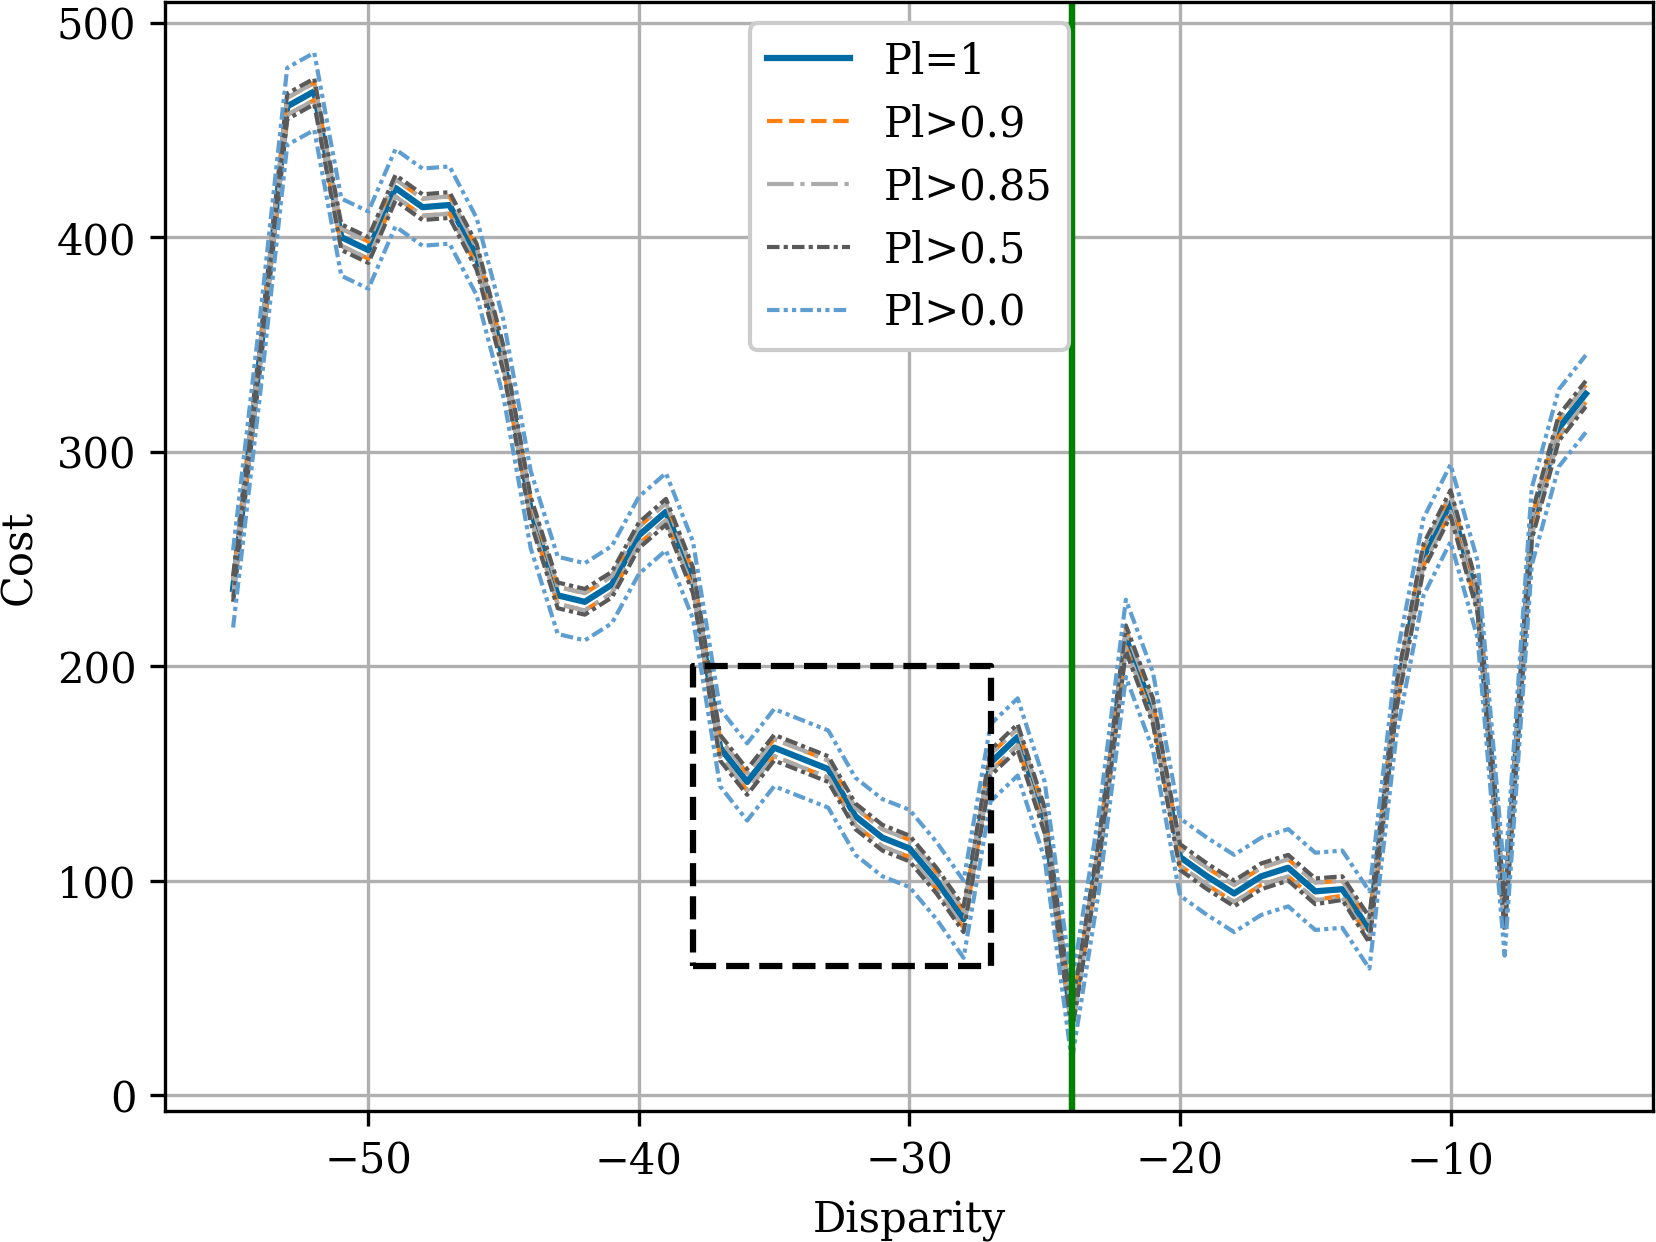
\includegraphics[width=\linewidth]{Images/Chap_4/bel_independence_100_120.png}
        \caption{$\SAD$ envelopes using the product Copula}
        \label{fig:belief_independence}
    \end{subfigure}\hfill
    \begin{subfigure}[t]{0.48\linewidth}
        \centering
        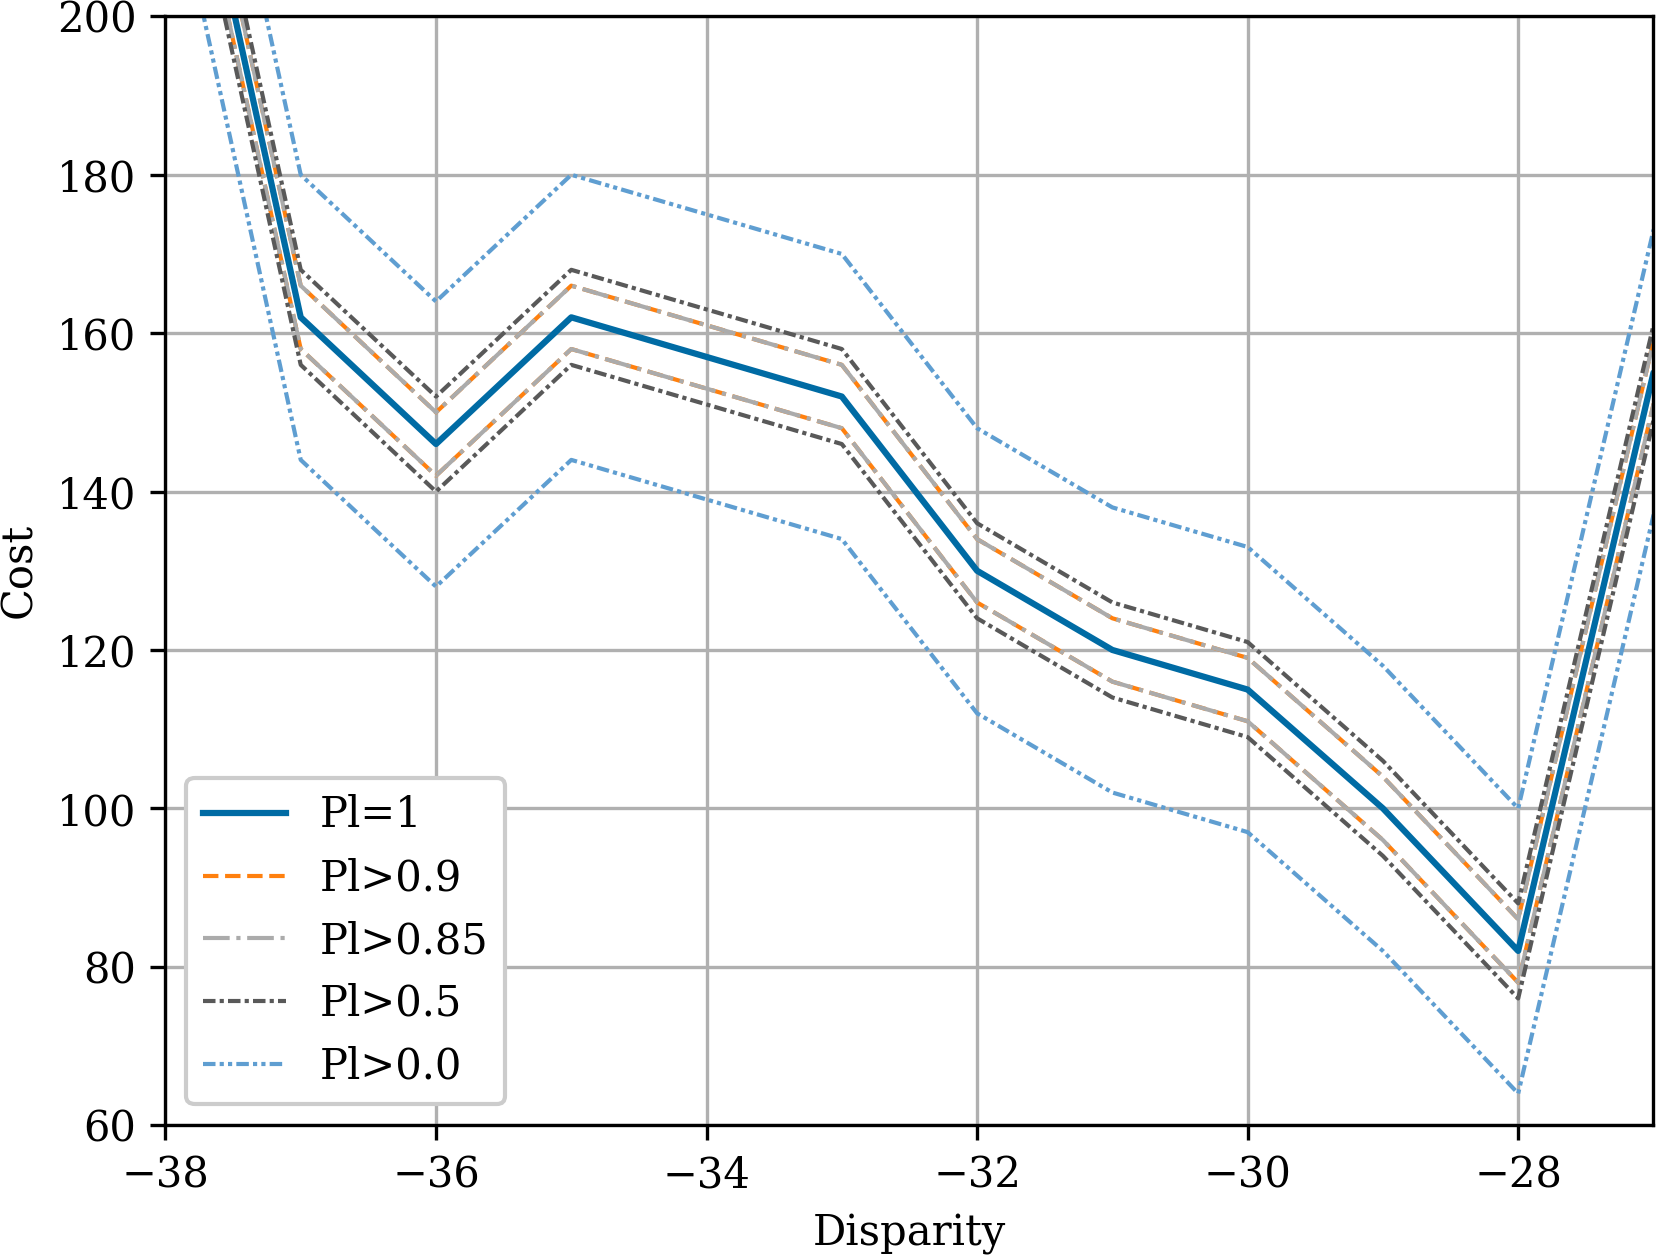
\includegraphics[width=\linewidth]{Images/Chap_4/bel_independence_100_120_zoom.png}
        \caption{Detailed view of the rectangular section of \ref{fig:belief_independence}}
        \label{fig:belief_independence_zoom}
    \end{subfigure}
    \begin{subfigure}[t]{0.48\linewidth}
        \centering
        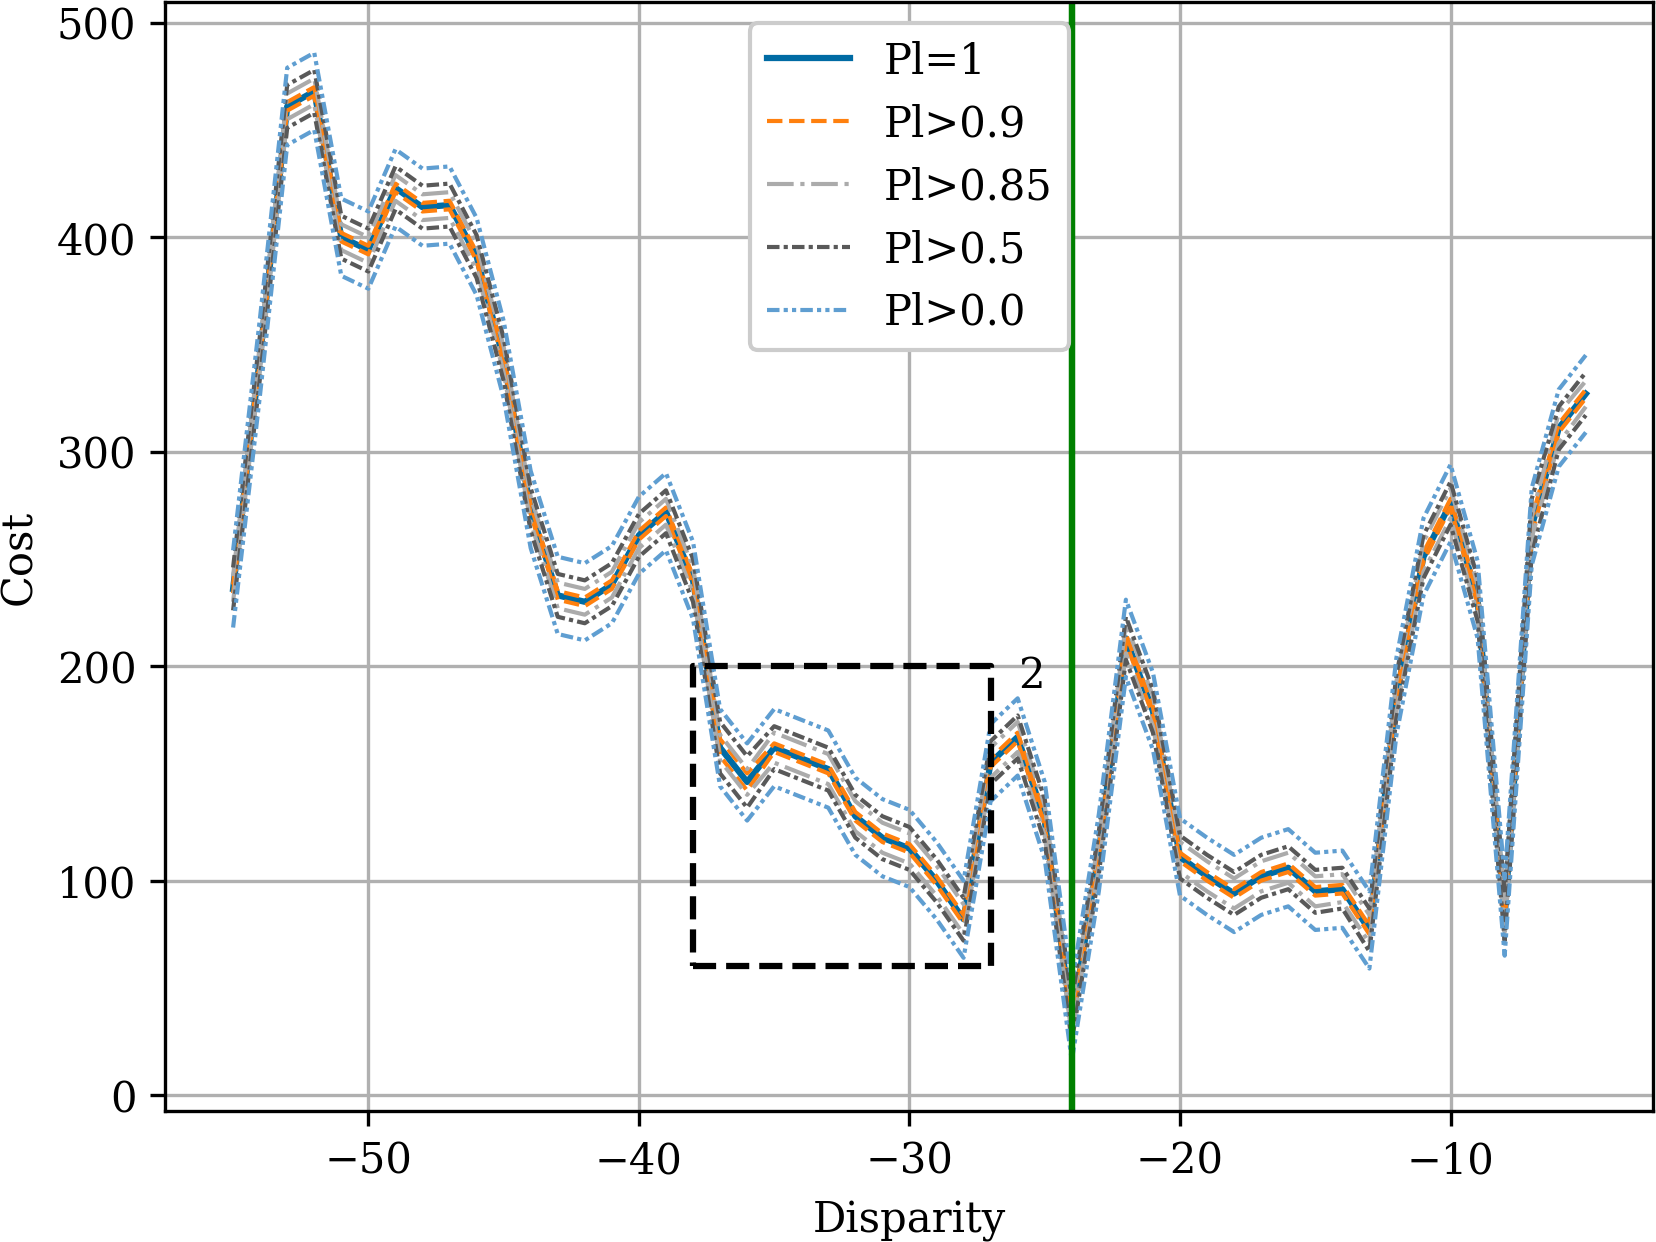
\includegraphics[width=\linewidth]{Images/Chap_4/bel_100_120.png}
        \caption{$\SAD$ envelopes using the Gaussian Copula}
        \label{fig:belief_gaussian}
    \end{subfigure}\hfill
    \begin{subfigure}[t]{0.48\linewidth}
        \centering
        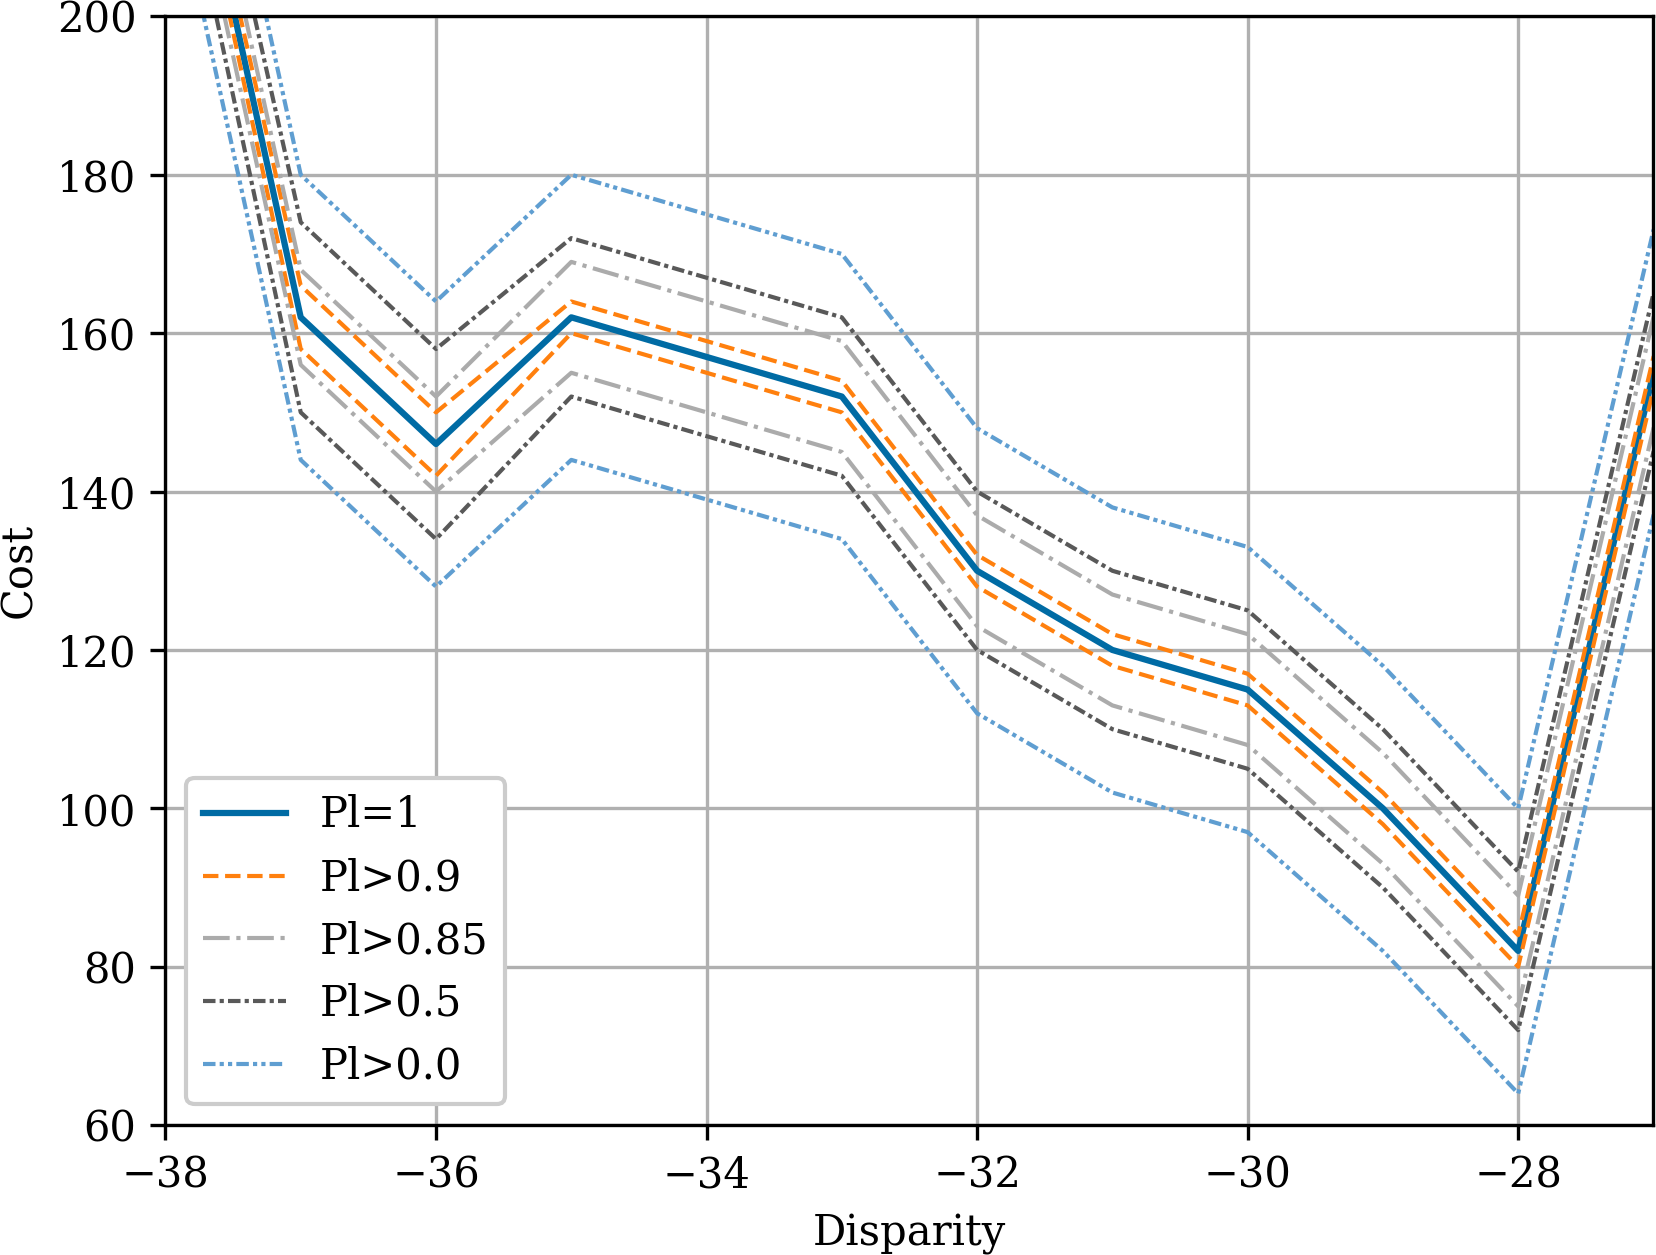
\includegraphics[width=\linewidth]{Images/Chap_4/bel_100_120_zoom.png}
        \caption{Detailed view of the rectangular section of \ref{fig:belief_gaussian}}
        \label{fig:belief_gaussian_zoom}
    \end{subfigure}
    \caption{Plausibility levels of a cost curve for the product copula $C_\Pi$ and the Gaussian copula $C_R$. The green vertical line represents the true disparity. Rectangular sections from the left figures are detailed on the right. From \cite{malinowski_uncertainty_2024}.}\commanue{j'ai pas l'impression que tu mentionnes à quel pixel ces courbes correspondent}
    \label{fig:belief_curves}
\end{figure}

A visualization of different plausibility levels of the $\SAD$ cost curve are presented in \Cref{fig:belief_curves}, computed with the product copula $C_\Pi$ and a Gaussian copula $C_R$. Both copula have the same support $\Pl>0$, and the same value for $\Pl=1$. Envelopes of the other plausibility levels are however different. \Cref{fig:belief_independence_zoom} and \Cref{fig:belief_gaussian_zoom} display the fact that the values covered by the plausibility levels vary with the copula used. Plausibility levels $0.85$ and $0.5$ are more concentrated around plausibility level $1$ in the case of the product copula than in the case of the Gaussian copula. Conversely, plausibility level $0.9$ is closer to plausibility level $1$ in the case of the Gaussian copula. This is due to the fact that the Gaussian copula $C_R$ is more co-monotone than the product copula given the correlation matrix $R$ described in \cref{eq:correlation}\commanue{là tu pointes sigma et pas R a priori c'est pas le bon label}.
\begin{remark}
    Both the Gaussian and the product copula have the same support. This is because when computing the joint mass of marginal focal sets, the copula is regular enough to assign a non-null mass to every focal set. This would not have been the case if we took a copula close to the lower or upper Fréchet-Hoeffding bound (the lower bound is not a copula for $n>2$). Indeed, those copulas are less regular, and can assign a null mass to joint events, as we saw in the case of probabilities in example \ref{ex:copulas} and more recently in example \ref{ex:propagated_probability}.
\end{remark}

\subsection{Estimating Propagated Credal Sets Using Monte Carlo Sampling}\label{sec:montecarlo}
In \Cref{chap:joining_credal_sets}, we defined $3$ methods for creating multivariate credal sets: $\M_{robust}$, $\M_{mass}$ and $\M_{agg}$. In the case where marginals were possibility distributions, we saw that the bounds of $\M_{agg}$ and $\M_{mass}$ were the same on Cartesian products, so we only considered $\M_{mass}$ in our application. In the previous sections, we propagated the uncertainty by using the approach from $\M_{mass}$. In this section, we will try to estimate the propagated uncertainty using $\M_{robust}$, and compare it to previous results so as to evaluate whether or not we can use $\M_{mass}$ to outer/inner approximate $\M_{robust}$.

We remind here some definitions and results regarding $\M_{robust}$. $\M_{robust}$ is the convex hull $CH$ of the set of every CDF from $n$ marginal credal sets $\M_i$ (in our case $n=18$, one per pixel involved in the $\SAD$ computation) joined with a copula $C$ (\cref{eq:robust_set}):
\begin{align*}
    \M_{robust} = CH(\{F=C(F_1 \enum F_n),~F_i\in\M_i \})
\end{align*}
We can estimate $\M_{robust}$ using Monte Carlo samplings: we first generate marginal probability distributions $F_1\enum F_n$ belonging in their respective marginal credal sets \cite{troffaes_note_2017}, then sample from the joint CDF $F$\commanue{Donc là c'est la version résumé et ensuite tu détailles donc il faudra mettre un petit mot de tarnsition. Je sais pas To do so ou IN detail ou un autre choix}. For each of the $18$ considered pixels, we sample a marginal CDF $F_i$ belonging to the credal set defined in \cref{eq:pixel_possibility}. The sampling from credal sets is not random: we generate probability distributions in such a way that for each marginal event $A$, the probability range $[\Nec(A), \Pi(A)]$ is sampled uniformly. With this method, we get a good coverage of each marginal credal set. We are also insuring that lower and upper bounds on events are all reached at least once, in order to include ``extreme'' distributions in our simulations. Once we have a CDF $F_i$ from each marginal CDF $F_i$, we can sample from the joint CDF using the method detailed in \Cref{sec:sampling_copula}. This yields a noised version of both left and right images, where the noised dependency is modeled by the provided copula, and its distribution is coherent with the possibility distributions from \cref{eq:pixel_possibility}. We can then compute a noised version of the cost volume from those images. For each cost curve, this provides a Monte Carlo samples of the $\SAD$ cost curves.

We compute $10\,000$ samples CDFs from each marginal credal set to construct the multivariate CDF. Each multivariate CDF is then itself sampled $10\,000$ times. The Central Limit Theorem states that $N$ Monte Carlo samples gives you an approximation with a precision of around $\frac{1}{\sqrt{n}}$\commanue{pourquoi le n est petit dans la formule ?} (it also depends on the standard deviation of the density you are estimating, but it is a good enough approximation), so $N=10\,000$ provides a satisfying precision for our application.  

In practice, we do not simulate a full noised pair of images at once, as it would require to sample from a copula of very large dimension (the number of pixels in both images). This is not realistically feasible, even thought it would ensure that each time a pixel is considered in the cost volume, the same noise samples are used. We instead generate noise samples for each row separately: noised values of pixels will not change during the evaluation of a cost curve for different disparities, or between the cost curves of pixels of the same row. However, their values might change between cost curves of pixels belonging to different rows. For instance, let's consider a pixel $p=(row,~col)\in I_L$ for which we computed a noised intensity $i_p$. We will use the same noised value $i_p$ of intensity when computing the $\SAD$ of every pixel $q=(row,~col')\in I_L$. But when computing the $\SAD$ of every pixel $q=(row-1,~col')\in I_L$, we will use a different Monte Carlo draw $i_p'$ for its intensity, which will stay the same for every pixel of row $row-1$. Because we draw a high number of Monte Carlo draws for each row, proceeding as such should not be noticeable. 

\begin{remark}
    As we construct the correlation matrices $R$ based on the segmentation of the left and right images, the cost curves presented in \Cref{fig:montecarlo_gauss_100_120,fig:montecarlo_gauss_200_150} mostly use a different copula for each disparity. Providing the values of those matrices would necessitate to represent around $60$ $18\times18$ correlation matrices, and is thus not provided here.
\end{remark}

\begin{figure}
    \centering
    \begin{subfigure}[t]{1\linewidth}
        \centering
        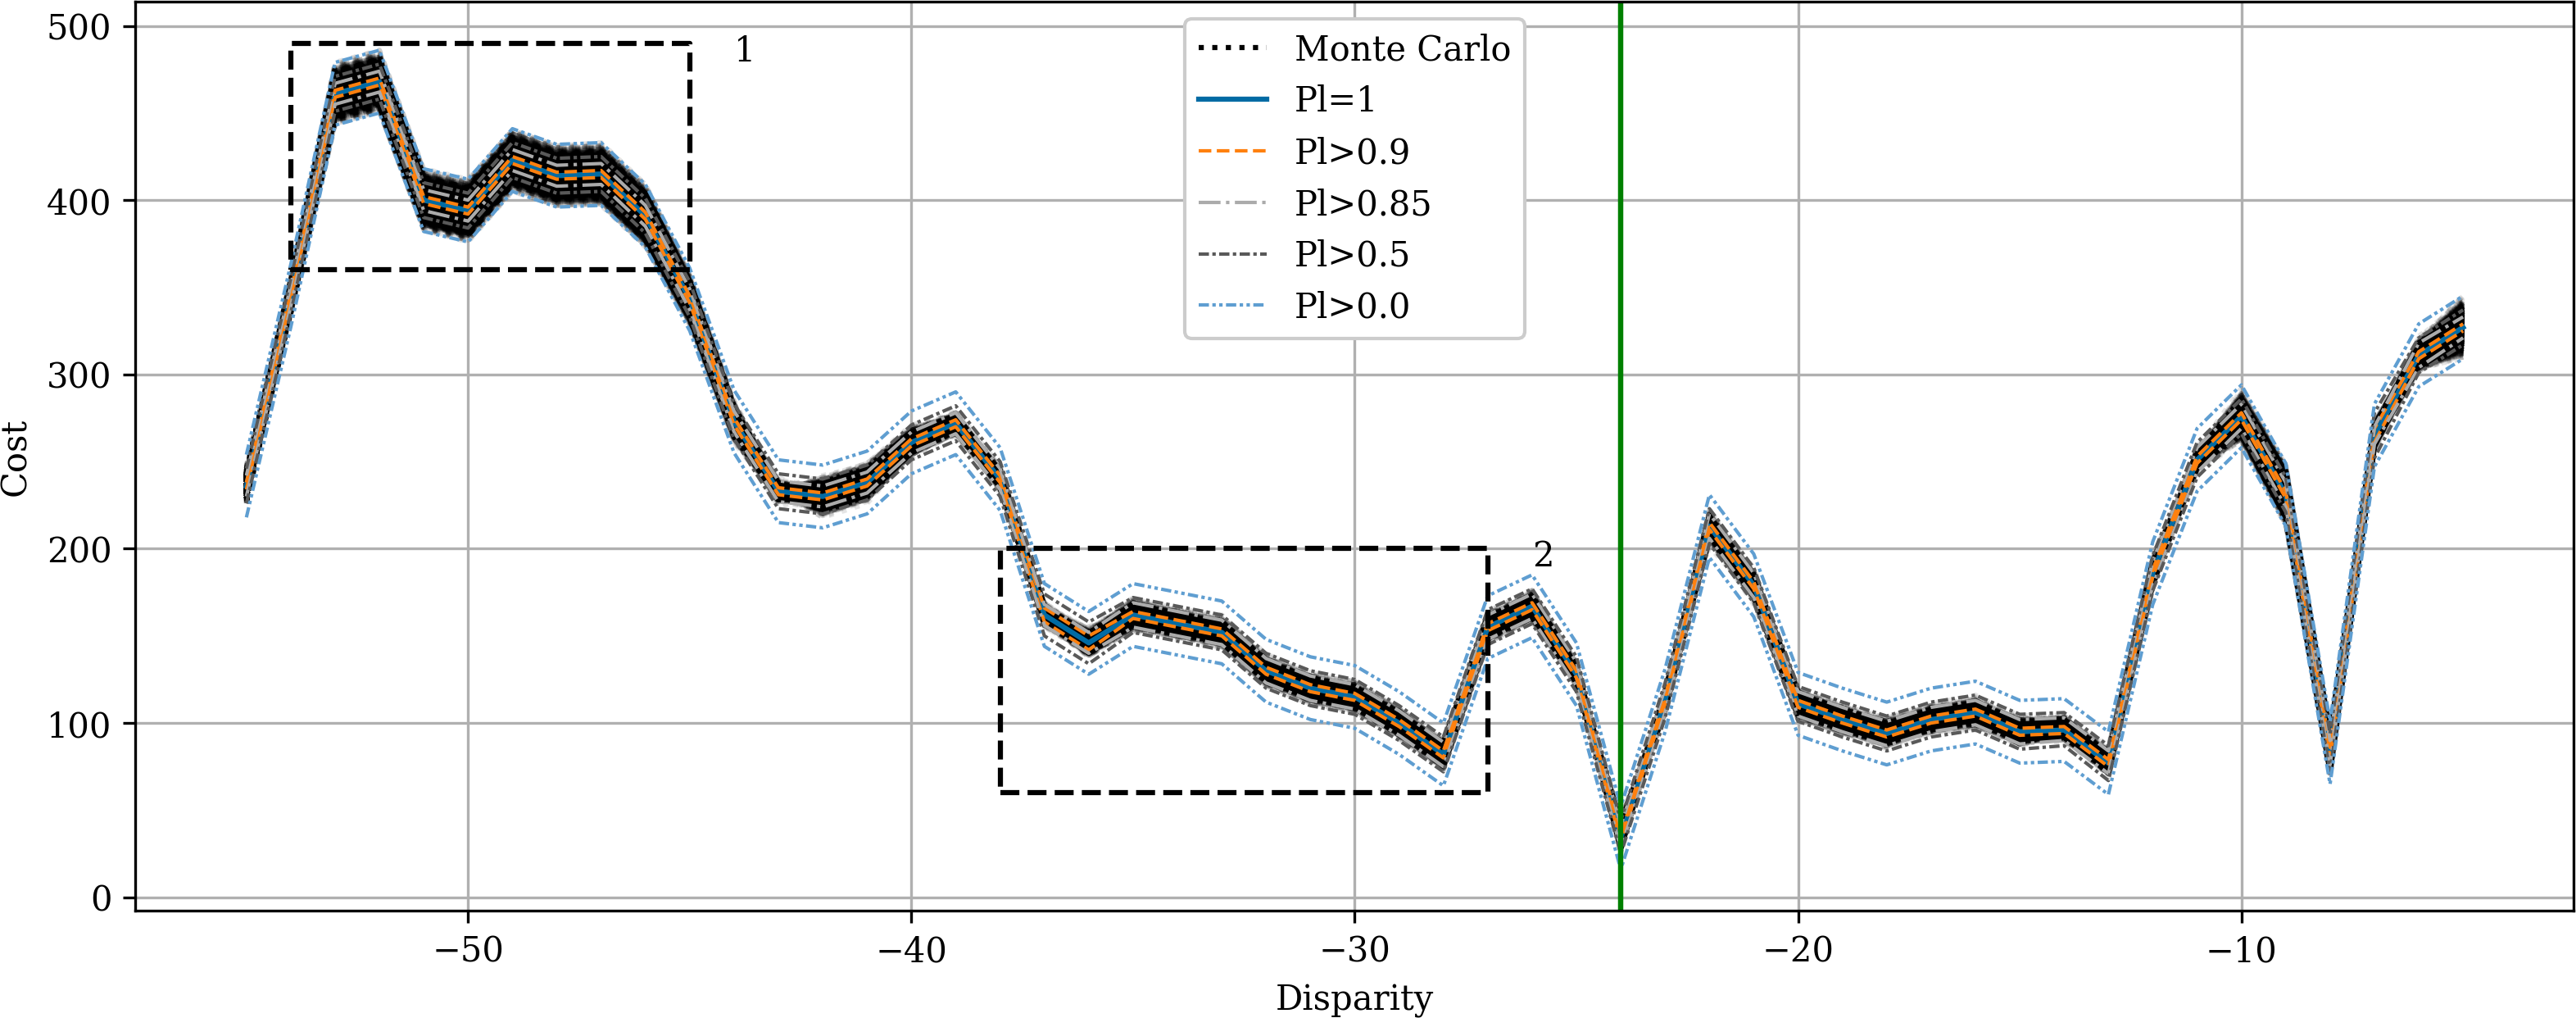
\includegraphics[width=\linewidth]{Images/Chap_4/cost_curve_100_120.png}
        \caption{Plausibility levels and Monte Carlo sampling using a Gaussian copula}
        \label{fig:montecarlo_gauss_100_120_large}
    \end{subfigure}\\
    \begin{subfigure}[t]{0.45\linewidth}
        \centering
        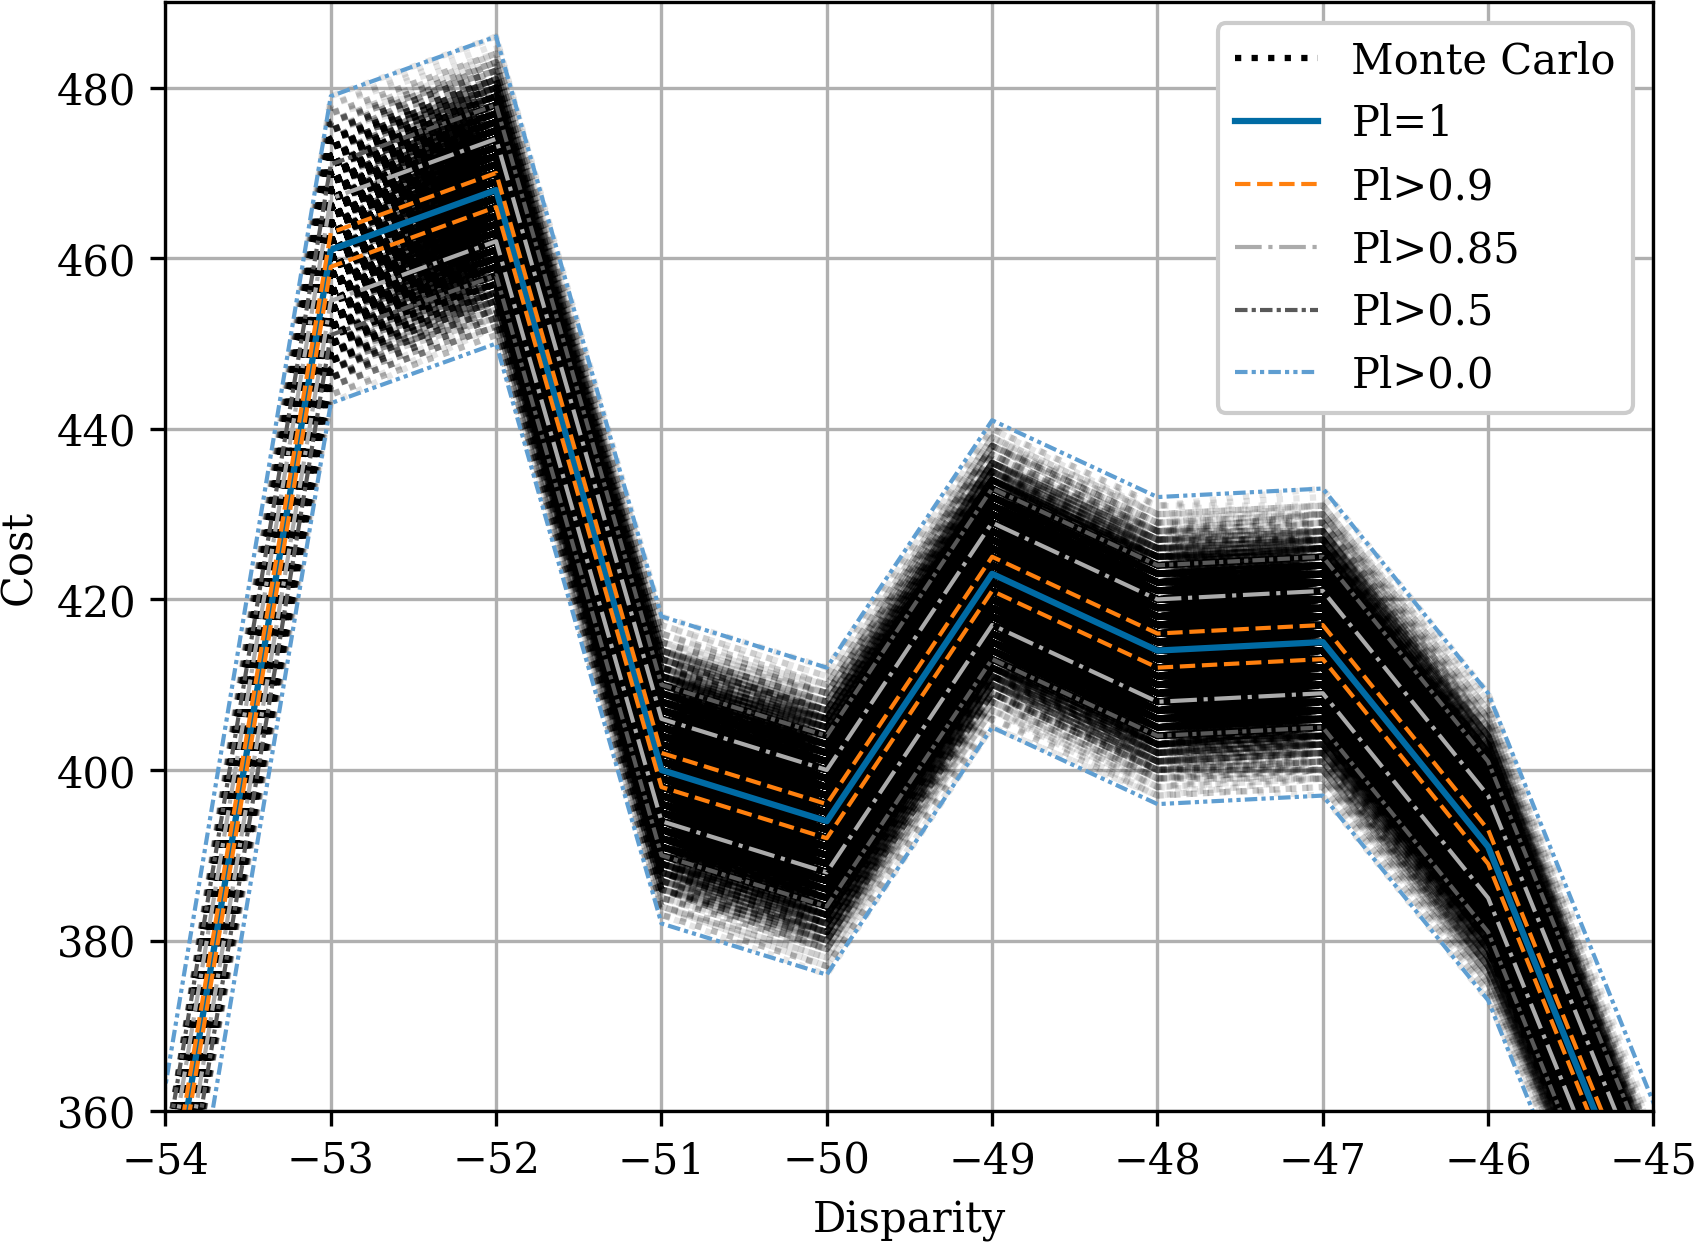
\includegraphics[width=\linewidth]{Images/Chap_4/cost_curve_100_120_zoom1.png}
        \caption{Zoom over the first rectangle}
        \label{fig:montecarlo_gauss_100_120_zoom1}
    \end{subfigure}\hfill
    \begin{subfigure}[t]{0.45\linewidth}
        \centering
        \includegraphics[width=\linewidth]{Images/Chap_4/cost_curve_100_120_zoom2.png}
        \caption{Zoom over the second rectangle}
        \label{fig:montecarlo_gauss_100_120_zoom2}
    \end{subfigure}
    \caption{Plausibility levels and Monte Carlo sampling for a pixel of the left image. From \cite{malinowski_uncertainty_2024}.}
    \label{fig:montecarlo_gauss_100_120}
\end{figure}

\begin{figure}
    \centering
    \begin{subfigure}[t]{\linewidth}
        \centering
        \includegraphics[width=\linewidth]{Images/Chap_4/cost_curve_200_150.png}
        \caption{Plausibility levels and Monte Carlo sampling using a Gaussian copula}
        \label{fig:montecarlo_gauss_200_150_large}
    \end{subfigure}\\
    \begin{subfigure}[t]{0.45\linewidth}
        \centering
        \includegraphics[width=\linewidth]{Images/Chap_4/cost_curve_200_150_zoom1.png}
        \caption{Zoom over the first rectangle}
        \label{fig:montecarlo_gauss_200_150_zoom1}
    \end{subfigure}
    \hfill
    \begin{subfigure}[t]{0.45\linewidth}
        \centering
        \includegraphics[width=\linewidth]{Images/Chap_4/cost_curve_200_150_zoom2.png}
        \caption{Zoom over the second rectangle}
        \label{fig:montecarlo_gauss_200_150_zoom2}
    \end{subfigure}
    \caption{Plausibility levels and Monte Carlo sampling for a pixel of the left image.  From \cite{malinowski_uncertainty_2024}.}
    \label{fig:montecarlo_gauss_200_150}
\end{figure}

Monte Carlo draws using the Gaussian copula and marginals credal sets of \cref{eq:pixel_possibility} are plotted in \Cref{fig:montecarlo_gauss_100_120,fig:montecarlo_gauss_200_150}. They respectively correspond to the cost curves of pixel located at positions $(100,~120)$ and $(200,~150)$ on the left image\commanue{alors les deux figures ont actuellement la même légende tu pourrais préciser la localisation du pixel dans la légende et cerise sur le gateau tu pourrais afficher l'image des cônes ou dire à quoi correspondent les deux pixels choisis car perso moi je ne sais pas à quel endroit ça correspond.}. Plausibility levels from \Cref{fig:belief_curves}\commanue{est-ce qu'il ne faudrait pas dire que tu affiches les plausibility levels de ces pixels calculés comme décrit pécédemment car dans la figure 4.4 tu ne considères qu'un seul pixel} also appear for comparison. The support envelopes from plausibility levels $\Pl>0$ correctly contain all Monte Carlo samplings for all considered copulas. We can observe in \Cref{fig:montecarlo_gauss_200_150_zoom2} that plausibility levels sometimes fail to correctly grasp the fluctuations of the dispersion of the samples, even though they correctly contain Monte Carlo samples. More specifically, Monte Carlo draws are first dense around disparity $-37$, then seem to spread around $-35$, and finally regather around disparity $-32$. The plausibility envelopes are more regular in this disparity range. This illustrates the fact the ``true'' point-wise credal $\M_{robust}$ set described in \Cref{sec:robust_method} is different from the joint credal set $\M_{mass}$ from \Cref{sec:joint_mass}. 

Although some differences persist between those sets, \Cref{fig:montecarlo_gauss_100_120_zoom2,fig:montecarlo_gauss_200_150_zoom2} suggest that the point-wise credal set $\M_{robust}$ can be outer approximated by $\M_{mass}$ in our applications. To quantify this observation, we can compute the proportion of Monte Carlo samples contained inside the plausibility envelopes for different plausibility levels $\gamma$:
\begin{align}
    \textrm{coverage}_\gamma = \frac{\#\{\textrm{ Monte Carlo samples }\in[\underline{I}_\gamma,~\overline{I}_\gamma]\}}{\#\{\textrm{ Monte Carlo samples }\}}
\end{align}
The coverage for the considered values of $\gamma$ are presented in \Cref{tab:Coverage}, where the first two rows represent the coverage of \Cref{fig:montecarlo_gauss_100_120,fig:montecarlo_gauss_200_150}. The global coverage over the whole left image is presented in the last row of the table. The coverage is always $100\%$ for $\gamma=0$, which shows that every sample is contained inside the support envelopes and that $\M_{robust}$ seems to be a subset of $\M_{mass}$. On the other hand, plausibility level $\gamma=0.5$ contain most Monte Carlo samples which means that the bounds could be significantly reduced while still being a good estimation of $\M_{robust}$. Finally, the variation of the coverage for plausibility levels $0.85$ and $0.9$ translates the previous observation that $\M_{mass}$ does not capture the variations of $\M_{robust}$ bounds and that those two set can substantially differ. Having estimated the uncertainty of the cost volume, we will see in the following section how we can leverage the upper and lower bounds for different plausibility levels to improve the disparity map derived from the cost volume.  

\begin{table}[ht]
\centering
\begin{tabular}{|c|c|c|c|c|}
\hline
\rowcolor[HTML]{C0C0C0}
$p=(row,col)$ & $\gamma=0.9$  & $\gamma=0.85$ & $\gamma=0.5$  & $\gamma=0$   \\ \hline
\cellcolor[HTML]{C0C0C0}$(100,~120)$     & $64,5\%$ & $94,5\%$ & $99,0\%$ & $100\%$ \\ \hline
\cellcolor[HTML]{C0C0C0}$(200,~150)$     & $30,0\%$ & $82,6\%$ & $95,2\%$ & $100\%$ \\ \hline
\cellcolor[HTML]{C0C0C0}Global        & $41,1\%$ & $87,6\%$ & $96,8\%$ & $100\%$ \\ \hline
\end{tabular}
\caption{Average coverage for various plausibility levels $\gamma$ and for different pixels $p$ of the left image.}\label{tab:Coverage}
\end{table}

\subsection{Leveraging Confidence Envelopes for Potential Improvements}\label{sec:sad_improvements}

Knowing the uncertainty, represented as confidence envelopes in our case, can provide valuable insights into potential matches. This section outlines different observations suggesting that incorporating this information can enhance the performance of stereo-matching algorithms.

From the cost volume $C_V$, we usually apply a \textit{winner-takes-all} strategy to compute a disparity prediction. Given a pixel $(row, ~col)$, the predicted disparity $\tilde{d}$ is defined as:
\begin{align}\label{eq:winner_takes_all}
    \tilde{d}(row, ~col) = \argmin_{d}C_V(row, ~col, ~d)
\end{align}
A common metric for evaluating stereo algorithm performance is the proportion of pixels for which the absolute difference between the true disparity $d_{true}$ and the predicted disparity $\tilde{d}$ is less than one pixel. The score \( s \) is defined as:
\begin{equation}\label{eq:score_d1}
    s = \frac{\#\{(row, col) \text{ such that } |d_{\mathrm{true}}(row, col) - \tilde{d}(row, col)| < 1\}}{\#\{(row, col)\}}\,.
\end{equation}
This metric is used as we usually only consider integer disparities (otherwise we need to upsample the stereo images\commanue{oui alors là c'est un peu un raccourci dans le remarque, vu ton pipeline (pas de raffinement) tu es sur des disparités entières. Mais la métrique elle est valable sur ce qu'on veut.}) but the ground truth disparity can be any real number in the disparity range\commanue{bah tu peux utiliser cette métrique avec n'importe quelle valeur de seuil. Là question est de savoir quelle est la précision de ta VT. Bref je comprends pas trop la phrase.}. We thus consider a disparity to be ``correct'' if it is less than one pixel away from the true disparity.

Having computed envelopes $\underline{I}_\gamma$, $\overline{I}_\gamma$ on the cost volume for different plausibility levels $\gamma$, the cost curve is not unique anymore, and we can instead consider all cost curves $C_{\underline{I}_\gamma,\overline{I}_\gamma}$ contained within the plausibility envelopes. Instead of a single predicted disparity, we can now compute the set of all potential disparities, defined as the set of predicted disparities from every cost curve contained in the plausibility envelopes. Given a pixel $(row, col)$, a confidence level $\gamma \in [0, 1]$, and plausibility envelopes $\underline{I}_\gamma(row, ~col, ~d)$, $\overline{I}_\gamma(row, ~col, ~d)$, the set of potential disparities $D_\gamma^{row, col}$ is defined as\commanue{Il y a un signe $\leqslant$ au milieu d'un intervalle}:
\begin{align}
    D_\gamma^{row, col} = \{d \mid& d=\argmin_\delta C_{\underline{I}_\gamma,\overline{I}_\gamma}(row,~col,~\delta),\\
    &\forall C_{\underline{I}_\gamma,\overline{I}_\gamma}(row, ~col, ~\delta)\in[\underline{I}_\gamma(row, ~col, ~\delta)\leqslant \overline{I}_\gamma(row, ~col, ~\delta)]\}\nonumber
\end{align}
There is actually a simpler way of defining and computing $D_\gamma$, which is to notice that a disparity can be the minimum of a cost curve $C_{\underline{I}_\gamma,\overline{I}_\gamma}$ if and only if the lower bound $\underline{I}_\gamma$ for this disparity is less than every upper envelope $\overline{I}_\gamma$\commanue{je comprends pas le terme every upper enveloppe. Tu fixes gamma et donc tu regardes qu'une seule enveloppe et tu t'assures que tu sois en dessous du min de la borne sup, ou alors j'ai rien compris}:
\begin{equation}
    D_\gamma^{row, col} = \{d \mid \underline{I}_\gamma(row, ~col, ~d) \leq \min_\delta\overline{I}_\gamma(row, col, \delta)\}
\end{equation}
\Cref{fig:potential_disparities} provides a schematic example of $D_\gamma(row, col)$.
\begin{figure}[ht]
    \centering
    \includegraphics[width=\linewidth]{Images/Chap_4/Potentiel_disparities.png}
    \caption{Example of a set of potential disparities $D_\gamma$. The minimum of the upper envelope $\min\overline{I}_\gamma$ in dashed gray line. The vertical green line represents the true disparity.}
    \label{fig:potential_disparities}
\end{figure}

When the cost volume is considered without its uncertainty, many disparities are not correctly estimated by \cref{eq:winner_takes_all}. We thus want to quantify the potential score improvements contained in the set of potential disparities $D_\gamma$. To do so, we consider that $D_\gamma$ is a potential improvements if it contains the true disparity $d_{true}$. From this we can compute the proportion of potential improvements $s_\gamma^{\text{opt}}$ over the whole image, and compare it to the score $s$ computed without uncertainty from \cref{eq:score_d1}. The proportion of potential improvements, or optimal score, \( s_\gamma^{\text{opt}} \) achievable using the set of possible disparities is computed as follows\commanue{là ça fait redite donc introduis et définis ton score optimal et ensuite tu dis que tu le compares. Là tu introduis, dis que tu vas le comparer et ensuite tu le définis. C'est le tiercé dans le désordre.}:
\begin{equation}\label{eq:optimal_score}
    s_\gamma^{\text{opt}} = \frac{\#\{(row, col) \mid \min_{d \in D_\gamma^{row, col}} |d_{\mathrm{true}}(row, col) - d| < 1\}}{\#\{(row, col)\}}
\end{equation}
In \Cref{fig:potential_disparities}, we can see that the predicted disparity $\tilde{d}$ is far away from the true disparity $d_{true}$, but the set of possible disparity $D_\gamma$ does indeed contain, the true disparity. This would have been counted as a potential improvement.

\begin{remark}
    \Cref{eq:optimal_score} defines the optimal score that \textit{could} have been obtained if we used an ideal cost volume contained in the envelopes. We do not provide a method for determining this ideal cost volume. In reality, even with a good strategy to leverage uncertainty information to obtain a better disparity map, the new score $s$ from \cref{eq:score_d1} would be lower than $s_\gamma^{\text{opt}}$.
\end{remark}

We define the potential gain as \( \Delta s_\gamma = s_\gamma^{\text{opt}} - s \). $\Delta s_\gamma$ measures the proportion of pixel that benefit from the method, \ie pixels $(row, ~col)$ verifying:
\begin{equation}
    |d_{\mathrm{true}}(row, ~col) - \tilde{d}(row, ~col)| \geq 1 \quad \text{and} \quad \min_{d \in D_\gamma^{row, col}} |d_{\mathrm{true}}(row, ~col) - d| < 1
\end{equation}

Examples of optimal scores and potential gains for various $\gamma$ values are provided in \Cref{tab:optimal_score}. We can see that while the potential gain for $\gamma = 0.9$ is low, it increases significantly for lower values of $\gamma$. The base score is around $53\%$, which is a relatively low score for dense matching, but that was expected as we are using the $\SAD$ without \acrshort{sgm} regularization or additional post processing. With $\gamma=0.85$, we could reach an optimal score of $67\%$, and using $\gamma=0.5$ or $\gamma=0$, the score could at best lie between $74\%$ and $82\%$. This is a quite significant improvement for a cost volume computed with the $\SAD$ cost function. For comparison, a $\SAD$ cost volume regularized with \acrshort{sgm} algorithm would have a score $s$ of $68\%$.

\Cref{fig:improvements} displays the spatial distribution of pixels that can benefit from this method. Pixels in occluded regions, \ie pixels only appearing in one of the two images, are highlighted in orange. As occluded pixels cannot be improved as no true disparity exists, we do not consider them when computing the different statistics introduced in this section. Pixels where potential improvement can occur appear in blue.

We can see that pixels with potential improvements are not randomly distributed. These pixels are typically found in homogeneous areas where multiple disparities have low matching costs, where the cost curves would be similar to the one represented in \Cref{fig:montecarlo_gauss_200_150_large}.
\comroman{Avec le recul ça aurait aussi été intéressant de voir si le nombre de disparité ou la dispersion de $D_\gamma$ pouvait être une mesure de confiance, calculer la courbe d'erreur comme dans le papier sur l'amb}\commanu{à mettre en perspective donc...}. 

\begin{table}[ht]
\centering
\begin{tabular}{|c|c|c|c|c|}
\hline
\rowcolor[HTML]{C0C0C0} 
$s=52.87\%$                                & $\gamma=0.9$ & $\gamma=0.85$ & $\gamma=0.5$ & $\gamma=0$ \\ \hline
\cellcolor[HTML]{C0C0C0}$s_\gamma^{opt}$   & $56.92\%$    & $66.99\%$     & $74.28\%$    & $81.75\%$  \\ \hline
\cellcolor[HTML]{C0C0C0}$\Delta s_\gamma$ & $4.05\%$     & $16.11\%$     & $21.41\%$    & $28.87\%$  \\ \hline
\end{tabular}
\caption{Optimal score and potential gain for different plausibility $\gamma$. The potential gain is computed with regards to the usual score $s=52,87\%$.}\label{tab:optimal_score}
\end{table}

\begin{figure}[ht]
    \centering
    \begin{subfigure}[t]{0.48\linewidth}
        \centering
        \includegraphics[width=\linewidth]{Images/Chap_4/Improvements_Pl=0.9.png}
        \caption{$\gamma=0.9,~\Delta s_\gamma=4.05\%$}
        \label{fig:improvements_a}
    \end{subfigure}
    \begin{subfigure}[t]{0.48\linewidth}
        \centering
        \includegraphics[width=\linewidth]{Images/Chap_4/Improvements_Pl=0.85.png}
        \caption{$\gamma=0.85,~\Delta s_\gamma=16.11\%$}
        \label{fig:improvements_b}
    \end{subfigure}\\
    \begin{subfigure}[t]{0.48\linewidth}
        \centering
        \includegraphics[width=\linewidth]{Images/Chap_4/Improvements_Pl=0.5.png}
        \caption{$\gamma=0.5,~\Delta s_\gamma=21.41\%$}
        \label{fig:improvements_c}
    \end{subfigure}
    \begin{subfigure}[t]{0.48\linewidth}
        \centering
        \includegraphics[width=\linewidth]{Images/Chap_4/Improvements_Pl=0.0.png}
        \caption{$\gamma=0,~\Delta s_\gamma=28.87\%$}
        \label{fig:improvements_d}
    \end{subfigure}
    \caption{Spatial disposition of potential improvements for different values of $\gamma$. Pixels with potential improvements appear in blue. Occluded pixels, for which a correct disparity does not exist, appear in orange. Grayscale left image is displayed on the background. From \cite{malinowski_uncertainty_2024}.}
    \label{fig:improvements}
\end{figure}

In this Chapter\commanue{oh mon dieu une conclusion, j'ai pas l'habitude, peut-être faire une section dédiée, c'est toi qui voit}, we modeled the uncertainty on stereo images and propagated it until the cost volume. We compared different methods from \Cref{chap:joining_credal_sets} for propagating the uncertainty, and evaluated the potential improvements unlocked by this uncertainty estimation. However, the stereo algorithm considered for computing the cost volume was intentionally simple to reduce the complexity of the problem. For the \acrshort{co3d} mission, different cost functions (CENSUS, MC-CNN) and \acrshort{sgm} regularization would instead be used. Furthermore, although the uncertainty on input images have an influence on the final uncertainty, the major part of the disparity map uncertainty comes from the processing uncertainty of the stereo algorithm itself. Quantifying and propagating this processing uncertainty will be thus be the subject of \Cref{chap:epistemic_uncertainty}.

\pagebreak
\blankpage
    
    \setkeys{Gin}{draft=true}
    \chapter{Computing Disparity Intervals and Propagate them to the DSM}\label{chap:epistemic_uncertainty}
\todoroman{Citer la publication d'origine pour les figure (license IEEE ``Copyright 2024 IEEE. Published in the 2024 IEEE International Geoscience and Remote Sensing Symposium (IGARSS 2024), scheduled for 7 - 12 July, 2024 in Athens, Greece. Personal use of this material is permitted. However, permission to reprint/republish this material for advertising or promotional purposes or for creating new collective works for resale or redistribution to servers or lists, or to reuse any copyrighted component of this work in other works, must be obtained from the IEEE. Contact: Manager, Copyrights and Permissions / IEEE Service Center / 445 Hoes Lane / P.O. Box 1331 / Piscataway, NJ 08855-1331, USA. Telephone: + Intl. 908-562-3966.'')}

The previous chapter detailed the propagation of  uncertainty in a stereo matching problem, using the $\SAD$ function to compute the cost volume. However, real cases of stereo matching usually do not use such simple cost functions, but rather more complex ones. In particular, the CARS pipeline that will process the \acrshort{co3d} data will use the CENSUS and MC-CNN cost functions  \cite{zabih_non-parametric_1994,zbontar_stereo_2016} to compute the cost volume, followed by a \acrshort{sgm} regularization. Those methods produce far better results and are thus favored for stereo pipelines. Unfortunately, we are not able to propagate the uncertainty to those cost functions and regularization as we did in the previous chapter as it would be too complex and computationally heavy. The same observation can be made for any deep leaning method \cite{laga_survey_2022} as the data is processed through many consecutive layers. Furthermore, the previous chapter was restricted to the propagation of the uncertainty from input images to the cost volume, but did not attempt to quantify the uncertainty of the stereo matching process itself, \ie the algorithm ability to correctly\commanue{properly? c'est pour éviter la répétition avec correct, à moins que ce soit voulu} identify the correct disparity. A bad performing stereo matching algorithm can produce errors of great magnitude regardless of the uncertainty on input images, while more advanced algorithm may even present good performance despite noised input images. Using the semantics of this thesis, we will refer to the uncertainty of the stereo algorithm itself as its epistemic uncertainty. Indeed, it does not result form any aleatoric process, but rather a lack of knowledge on how to correctly and automatically identify the correct disparity\commanue{pareil tu as une répétition entre correctly et correct dans la phrase}.

This aforementioned epistemic uncertainty\commanue{alors moi perso je mettrais This aforementioned epistemic uncertainty modeling in stereo matching mais c'est pas une obligation} has been the subject of many works in the literature \cite{hu_quantitative_2012,  poggi_confidence_2021,wang_uncertainty_2022}, designed for so-called ``classical methods'' using cost volumes obtained from cost functions, or for learning-based methods. This uncertainty is quantified using ``confidence measures'', associating a value between $0$ and $1$ to each predicted disparity, $0$ meaning that the prediction should be questioned,  and $1$ meaning that the prediction is most certainly correct. We refer to \Cref{sec:uncertainty_pandora} for more details on confidence measures in stereo matching pipelines. In this chapter, we will study how possibility distributions are able to model the epistemic uncertainty associated with a cost volume, and then deduce disparity confidence intervals from the possibility distribution. This approach is complementary to classical confidence estimations as it is not meant to indicate whether or not we trust a prediction but rather to provide information on \textit{where} the correct disparity should be. We then propagate those disparity confidence intervals in the rest of the stereo pipeline to obtain height confidence intervals, and evaluate their performances. Following discussions with users and experts working at CNES, IGN and more generally in the AI4GEO consortium, we decided to fix ourselves an objective of $90\%$ of correct confidence intervals.

\todoroman{Vérifier que dans le chapitre 1 j'insiste bien sur ce que c'est une cost curve}
\section{Producing Confidence Intervals}
This section will detail the method developed to create disparity confidence intervals in the stereo matching step of the pipeline. We will use possibility distributions to model the uncertainty associated with the available information and deduce confidence intervals from it.

It is important to keep in mind that we want intervals as precise as possible, while staying relatively small. Indeed, it would be easy to reach a $100\%$ precision by simply extending the intervals to the whole range of considered disparities. However, the intervals would not contain any relevant information. We therefore must maintain a trade-off between the precision of the intervals and their size. As stated previously, we fixed ourselves a $90\%$ precision objective. As for the criteria of maintaining small intervals, we will introduce in \Cref{sec:metrics_disparity} different metrics to quantify their size for further evaluation. Different parameters will be introduced in our method, and we chose their values accordingly with the precision/size trade-off mentioned above. We will also study different configuration of those parameters in annex. \todoroman{Mettre les analyses en annexe}

\subsection{Possibility Distributions as Uncertain Models for Cost Curves}
In this section, we will detail how possibility distributions can be used to model the epistemic uncertainty associated with cost curves. We first present a quick reminder of concepts and notations regarding cost volumes presented in \Cref{sec:stereo_matching}, as we will base our model on them. Cost volume based approaches, considered here, compare every pixel from the left image $I_L$ to pixels from the same row in the right image $I_R$, in a given disparity range. The comparison is done using a cost function $f$, measuring the dissimilarity between two windows centered around pixel $p$ and $q$. All evaluations using this cost function are stored in a cost volume $C_V$:
\begin{align}
	C_V(\rowcol, ~d) = f(I_L(\rowcol), I_R(\rowcol+d))
\end{align}
where $d$ is the considered disparity. In this chapter, we consider that the cost volume then\commanue{je mettrais pas le then} undergoes a \acrshort{sgm} regularization step, which modifies the cost values\commanue{its values} to take into account more global information. Based on the observation that the disparity map is usually piece-wise regular in a scene, \acrshort{sgm} regularization has been designed to increase the cost of disparities for which no consensus exist among neighboring pixels. This way, only disparities that seem plausible and relatively regular compared to neighboring disparities are favored in the cost volume.

For every pixel $(\rowcol)$ from the left image, we refer to its cost curve as the cost volume at coordinates $(row,~col)$ for every considered disparity $d$, \ie the cost volume for which we fixed the first two variables. Cost curves are of much importance as we estimate the disparity of a pixel solely based on its cost curve. Indeed, we define the predicted disparity $\tilde{d}$ of a pixel $(\rowcol)$ as:
\begin{align}
	\tilde{d} = \argmin_d C_V(\rowcol, ~d)
\end{align} 
\Cref{fig:tuto_dense_matching} presents a cost curve and its true disparity. We can see that the true disparity can be correctly estimated by looking at the minimum of the cost curve.
 
\begin{figure}
    \centering
    \begin{subfigure}[t]{0.073\linewidth}
        \centering
        \includegraphics[width=\linewidth]{Images/Chap_5/tuto_left_patch.png}
        \caption{}
        \label{fig:tuto_a}
    \end{subfigure}
    \hfill\begin{subfigure}[t]{\linewidth}
        \flushright
        \includegraphics[width=0.927\linewidth]{Images/Chap_5/tuto_right_patch.png}
        \caption{}
        \label{fig:tuto_b}
    \end{subfigure}
    \begin{subfigure}[t]{\linewidth}
        \centering
        \includegraphics[width=\linewidth]{Images/Chap_5/tuto_cost_curve.png}
        \caption{Cost curve}
        \label{fig:tuto_c}
    \end{subfigure}
    \caption{Cost curve (\Cref{fig:tuto_c}) obtained from comparing a patch from the left image (\Cref{fig:tuto_a}) to patches from the right image (\Cref{fig:tuto_b}). The matching patch and its corresponding true disparity are indicated using dashed green lines.}
    \label{fig:tuto_dense_matching}
\end{figure}

In the following, we propose to consider possibility distributions to model the uncertainty associated with the choice of the predicted disparity from a cost curve. The values taken by possibility distributions will be based on the available information \ie the values of the cost volume. Before getting into details, let us justify this model. Possibility distributions are relatively simple model to use in comparison with imprecise probabilities or belief functions for instance, as we only need to specify a constraint on the atoms, and not on every event. As such, they have been used to model the uncertainty associated with an expert's opinion in applications such as groundwater contamination for instance in \cite{bardossy_l-_1995} and \cite{baudrit_joint_2007}. Since cost curves result in both:
\begin{itemize}
	\item dissimilarity measures between patches 
	\item a semi-global fusion of the information contained in the cost volume due to \acrshort{sgm} regularization
\end{itemize}it does not seem far-stretched to consider them equivalent to an expert stating his opinion on how likely two pixels should be matched. For this reason, possibility distributions seem appropriate to model the epistemic uncertainty of the cost volume.

In order to use possibility distributions, we first need to transform the available information, in our case the values contained in the cost curves, into degrees of possibility. \Cref{eq:possibility}\commanue{Plutôt que de faire référence à une équation située 100 pages avant, tu pourrais juste dire The definition of possibility distribution ou un truc équivalent} imposes that the values must lie between $0$ and $1$, and that the value $1$ must be attained at least once. We therefore propose to normalize each cost curve so that its minimal dissimilarity value equals a possibility degree of $1$, and that greater dissimilarity values are closer to $0$ in possibility. However, simply normalizing the values of each cost curve between $0$ and $1$ would artificially stretch the cost curve as seen in \Cref{fig:cost_curves_b}. It is especially blatant in the case for the orange dashed curve from \Cref{fig:cost_curves_a} as the range of its values is quite narrow compared to the blue curve, but they are both stretched to $[0,~1]$ in \Cref{fig:cost_curves_b}. In order to avoid this effect, we instead normalize every cost curve using the global minimum and global maximum of the cost volume, as:
\begin{align}
	C_V^{norm}(\rowcol, ~d) = \dfrac{C_V(\rowcol, ~d) - \max_{r,c,\delta}C_V(r,~c,~\delta)}{\min_{r,c,\delta}C_V(r,~c,~\delta) - \max_{r,c,\delta}C_V(r,~c,~\delta)}\label{eq:normalized_cost_curve}
\end{align}
Minima of the cost curve become maxima with this normalization. One problem remains, it is that unless the global maximum of the cost volume is attained in a cost curve, the normalized cost curve will never reach $1$. Therefore, it will not be a possibility distribution. This problem can be observed in \Cref{fig:cost_curves_c}. We thus add a constant to the normalized cost curve to obtain a possibility distribution $\pi_{row,~col}(d)$:
\begin{align}
	\pi_{row,~col}(d) = C_V^{norm}(\rowcol, ~d) + 1 - \max_\delta C_V^{norm}(\rowcol, ~\delta)\label{eq:possibility_cost_curve}
\end{align}
\Cref{fig:cost_curves_d} displays the possibility distributions obtained from the cost curves of \Cref{fig:cost_curves_a}.

\begin{figure}
    \centering
    \begin{subfigure}[t]{0.47\linewidth}
        \centering
        \includegraphics[width=\linewidth]{Images/Chap_5/cost_curve_not_normalized.png}
        \caption{Two cost curves}
        \label{fig:cost_curves_a}
    \end{subfigure}\hfill
    \begin{subfigure}[t]{0.47\linewidth}
        \centering
        \includegraphics[width=\linewidth]{Images/Chap_5/cost_curve_bad_normalized.png}
        \caption{Normalized cost curves with local extrema}
        \label{fig:cost_curves_b}
    \end{subfigure}
    \begin{subfigure}[t]{0.47\linewidth}
        \centering
        \includegraphics[width=\linewidth]{Images/Chap_5/cost_curve_normalized.png}
        \caption{Normalized cost curves $C_V^{norm}$ with global extrema}
        \label{fig:cost_curves_c}
    \end{subfigure}\hfill
    \begin{subfigure}[t]{0.47\linewidth}
        \centering
        \includegraphics[width=\linewidth]{Images/Chap_5/cost_curve_possibility_distribution.png}
        \caption{Possibility distributions resulting from the cost curves}
        \label{fig:cost_curves_d}
    \end{subfigure}\hfill
    \caption{Transformation of cost curves (CENSUS + \acrshort{sgm} on Middlebury Cones) into possibility distributions. \Cref{fig:cost_curves_a} represents two cost curves that are normalized differently in \Cref{fig:cost_curves_b,fig:cost_curves_c}. \Cref{fig:cost_curves_d} uses the normalization of \Cref{fig:cost_curves_c} to create possibility distributions.}
    \label{fig:cost_curves_to_possibility}
\end{figure}

As stated previously, global extrema in \cref{eq:normalized_cost_curve} are employed to minimize the stretching effect when converting cost curves into possibility distributions. However, we also could have used the theoretical extrema of a cost curve instead. For instance, the CENSUS cost function on a $5\times5$ window provides values between $0$ and $C_{max}=24$. Adding \acrshort{sgm} regularization with penalty $P_2$ on $8$ directions yields cost volumes values between $0$ and $8\times(C_{max}+P_2)$ \cite{hirschmuller_accurate_2005}. However, this maximal cost is rarely attained in real case scenarios, and\commanue{je remplacerais and par therefore it} is too pessimistic and tends to over-compress the normalized cost curves. It is instead preferred to use global extrema of the cost volume for the normalization, as we suppose the best and worst match should have similar cost values across different scenes. This hypothesis is not restrictive for the images we consider in our stereo matching problem, as the size and diversity inside each scene lead to similar extrema. \todoroman{Faire relire la fin à Manue car le Balrog ne l'a pas lu} When processing very large images, CARS uses divide the image in smaller tiles that are process in parallel. We are not guaranteed that the cost volume extrema of each tile would be the same, but as they all come from the same image, it is not far-stretched to suppose differences in extrema are negligible. 

\subsection{From Possibilities to Disparity Confidence Intervals}
With the possibility distributions defined, our next objective is to establish a set of most possible disparities. We decided to aim for sets containing the true disparity $90\%$ of the time. This $90\%$ value was chosen following discussions with users and other experts working at CNES, IGN and more generally in the AI4GEO consortium. To define this set of most possible disparities, we compute the $\alpha$-cut (\cref{eq:alpha_cut}\commanue{tu fais un renvoi à l'équation, moi je renverrais à la définition. Bon c'est au même endroit de toute façon}) of the possibilities, or in other words, the set of all disparities $D_\alpha$ whose possibility is superior than $\alpha$:
\begin{align}
    D_\alpha=\{~ d ~|~ \pi_{\rowcol}(d)\geqslant\alpha\}\label{eq:set_of_possible_disparities}
\end{align}
By looking at possibility distributions obtained from different cost curves for which we know the true disparity, we first fixed the value $\alpha$ at $0.9$. In depth study of this parameter will be tested later, in order to see if it depends on the cost function, the type of scene considered, and to provide general guidelines on its optimal value. In the following, when the value of $\alpha$ is not specified, it will always be set at $0.9$. The fact that its value is the same as the $90\%$ confidence objective is a coincidence and one should not suppose that $\alpha$ and the confidence objective should be the same. Indeed raising the $\alpha$ value would decrease the size of the set $D_\alpha$ and therefore decrease the proportion of sets containing the true disparity, \ie the global confidence rate of intervals. \Cref{fig:disparity_intervals_a,fig:disparity_intervals_b} graphically represent $D_\alpha$ for the cost curves of \Cref{fig:cost_curves_to_possibility}.

\begin{remark}
    We are modelling the epistemic uncertainty of the cost curves using possibility distributions. In the rest of this chapter, we use a possibility distribution for each cost curve because we think it is a correct model in itself for the uncertainty we encounter. It is however possible to have a probabilistic interpretation of possibilities, which we will share in this remark as it may be of interest for people thinking the underlying uncertainty can be modeled by probabilities.
    
    We saw in \cref{eq:credal_set_possibility} from \Cref{chap:representation_of_uncertainty} that one way of interpreting $\pi_{\rowcol}$ is that it defines a set of probability distributions, \ie a credal set $\M$. We can also define $D_\alpha$ using this set $\M$, as:
    \begin{align}
        D_\alpha=\{~ d ~|~ \exists P\in\M ~\st~ P(d)\geqslant \alpha\}
    \end{align}
    or in plain words, $D_\alpha$ is the set of all disparities $d$ for which there exists a probability in $\M$ whose value is greater than $\alpha$ for $d$. We will not rely on this interpretation in the rest of this chapter, and instead only reason in terms of possibilities.
\end{remark}

\todoroman{Figure montrant différentes courbes de coût transformées, CENSUS MCCNN}

\Cref{eq:set_of_possible_disparities} defines a set of disparities $D_\alpha$ which is not necessarily convex. We will rather consider confidence disparity intervals $I_\alpha$ deduced from $D_\alpha$ in the rest of this chapter:
\begin{align}
    I_\alpha = [\underline{I}_\alpha,~\overline{I}_\alpha]=[\min D_\alpha, ~\max D_\alpha]\label{eq:confidence_disparity_intervals}
\end{align}
\Cref{fig:disparity_intervals_c,fig:disparity_intervals_d} graphically represent how $I_\alpha$ is determined for the two possibility distributions of the cost curves in \Cref{fig:cost_curves_to_possibility}. In the rest of this section, we will not make any distinction between disparity confidence intervals, disparity intervals, confidence intervals or simply intervals. A disparity interval is the convex envelope of its disparity set $D_\alpha$, which is a conservative approach as observed in \Cref{fig:disparity_intervals_b,fig:disparity_intervals_d}.

Considering intervals thus presents the advantage of working with convex sets and only requiring two scalars to describe the set. Users of the \acrshort{dsm}s produces by stereo photogrammetry are also used to consider confidence intervals \cite{oksanen_digital_2006, wang_robust_2015, panagiotakis_validation_2018, deschamps-berger_apport_2021, hugonnet_uncertainty_2022}. This will also facilitate further processing in the rest of the stereo pipeline, as we only need to take into account $2$ bounds to characterize the possible disparities, instead of a set of arbitrary shape. In the following figures, we use the same configuration for the correlator, \ie CENSUS cost function with \acrshort{sgm} regularization. We will study the influence of the cost function later\commanue{alors c'est bien de mentionner la conf utilisée. Après tant que tu utilises les figures juste à des fins explicatives c'est pas trop grave. Donc soit tu remontes cette info plus haut quand tu commences à faire des courbdes de coût. Soit tu gardes cette info quand tu en auras vraiment besoin pour valider ton approche. Histoire d'être sûr qu'entre temps les relecteurs n'aient pas oublié l'info. Là ça tombe un peu comme un cheveu sur la soupe dans ce paragraphe.}.

\begin{figure}
    \centering
    \begin{subfigure}[t]{0.47\linewidth}
        \centering
        \includegraphics[width=\linewidth]{Images/Chap_5/disparity_interval_1.png}
        \caption{$D_\alpha$ for the blue possibility of \Cref{fig:cost_curves_d}}
        \label{fig:disparity_intervals_a}
    \end{subfigure}\hfill
    \begin{subfigure}[t]{0.47\linewidth}
        \centering
        \includegraphics[width=\linewidth]{Images/Chap_5/disparity_interval_2.png}
        \caption{$D_\alpha$ for the orange possibility of \Cref{fig:cost_curves_d}}
        \label{fig:disparity_intervals_b}
    \end{subfigure}
    \begin{subfigure}[t]{0.47\linewidth}
        \centering
        \includegraphics[width=\linewidth]{Images/Chap_5/disparity_interval_3.png}
        \caption{$I_\alpha$ for the blue possibility of \Cref{fig:cost_curves_d}}
        \label{fig:disparity_intervals_c}
    \end{subfigure}\hfill
    \begin{subfigure}[t]{0.47\linewidth}
        \centering
        \includegraphics[width=\linewidth]{Images/Chap_5/disparity_interval_4.png}
        \caption{$I_\alpha$ for the orange possibility of \Cref{fig:cost_curves_d}}
        \label{fig:disparity_intervals_d}
    \end{subfigure}\hfill
    \caption{Set of possible disparities $D_\alpha$ and disparity intervals $I_\alpha$ with the same cost curves as in  \Cref{fig:cost_curves_to_possibility}, with $\alpha=0.9$. \Cref{fig:disparity_intervals_a,fig:disparity_intervals_b} represent the set of possible disparities $D_\alpha$ from \cref{eq:set_of_possible_disparities} in gray. \Cref{fig:disparity_intervals_c,fig:disparity_intervals_d} represent disparity intervals $I_\alpha$ from \cref{eq:confidence_disparity_intervals} in gray. There is no difference between $D_\alpha$ and $I_\alpha$ for the blue curve, contrary to the orange dashed curve.}
    \label{fig:disparity_sets_and_intervals}
\end{figure}

\begin{figure}
    \centering
    \includegraphics[width=0.5\linewidth]{Images/Chap_5/cones_with_rows.png}
    \caption{Left stereo image from Middlebury Cones. Disparity intervals $I_\alpha$ along orange lines are detailed in \Cref{fig:intervals_ambiguous_row_80,fig:intervals_ambiguous_row_180,fig:intervals_ambiguous_row_240,fig:intervals_ambiguous_row_290}}
    \label{fig:cones_with_rows}
\end{figure}\todoroman{Mettre qu'une seule ligne pour la théorie et rajouter les figures restantes dans la partie résultat}

To qualitatively evaluate the behaviour of disparity confidence intervals $I_\alpha$, we will look at their values for consecutive pixels of the same row. Considered rows\commanue{Rows selected for this analysis?} are presented in \Cref{fig:cones_with_rows}: the upper row ($80$) is smaller than the others so more details can be observed, while other rows allows for a broader view of the intervals\commanue{peut-être préciser si tu as pris les lignes au pif ou non.}.

\begin{figure}
    \centering
    \begin{subfigure}[t]{0.8\linewidth}
        \centering
        \includegraphics[width=\linewidth]{Images/Chap_5/intervals_ambiguous_area_row_80_1.png}
        \caption{$I_\alpha$ without regularization in low confidence areas}
        \label{fig:intervals_ambiguous_row_80_1}
    \end{subfigure}\hfill
    \begin{subfigure}[t]{0.8\linewidth}
        \centering
        \includegraphics[width=\linewidth]{Images/Chap_5/intervals_ambiguous_area_row_80_2.png}
        \caption{$I_\alpha$ with regularization in low confidence areas}
        \label{fig:intervals_ambiguous_row_80_2}
    \end{subfigure}
    \caption{$I_\alpha$ with and without regularization in low confidence area, for row $80$ of the image of \Cref{fig:cones_with_rows}. Low confidence areas are indicated by the gray areas.}
    \label{fig:intervals_ambiguous_row_80}
\end{figure}
\begin{figure}
    \centering
    \begin{subfigure}[t]{\linewidth}
        \centering
        \includegraphics[width=\linewidth]{Images/Chap_5/intervals_ambiguous_area_row_180_1.png}
        \caption{$I_\alpha$ without regularization in low confidence areas}
        \label{fig:intervals_ambiguous_row_180_1}
    \end{subfigure}\hfill
    \begin{subfigure}[t]{\linewidth}
        \centering
        \includegraphics[width=\linewidth]{Images/Chap_5/intervals_ambiguous_area_row_180_2.png}
        \caption{$I_\alpha$ with regularization in low confidence areas}
        \label{fig:intervals_ambiguous_row_180_2}
    \end{subfigure}
    \caption{$I_\alpha$ with and without regularization in low confidence area, for row $180$ of the image of \Cref{fig:cones_with_rows}. Low confidence areas are indicated by the gray areas.}
    \label{fig:intervals_ambiguous_row_180}
\end{figure}

By construction, $I_\alpha$ will always contain the predicted disparity $\tilde{d}$ as the maximum of each possibility curve will also be selected as the predicted disparity by winner-takes-all strategy. However, We are interested to see if intervals can contain the true disparity $d_{true}$ even when the predicted disparity is far from it. \Cref{fig:intervals_ambiguous_row_80_1,fig:intervals_ambiguous_row_180_1,fig:intervals_ambiguous_row_240_1,fig:intervals_ambiguous_row_290_1} represent the disparity intervals $I_\alpha$, predicted disparity $\tilde{d}$ and true disparity $d_{true}$ for the different rows. A first observation is that intervals correctly contain the true disparity in regions were there are no strong variations of disparities. In  \Cref{fig:intervals_ambiguous_row_180_1}, the intervals in columns $50$ to $75$ and around $175$ are much larger than in the rest of the figure. In those areas, the predicted disparity is also far from the ground truth. This translates the fact that the method for creating intervals is able to detect the difficulties encountered by the correlator when predicting a disparity, and to adapt the intervals size consequently. On the downside, we can see that near strong variations of the disparity, the intervals tend to ``miss'' the discontinuities. Indeed, they do not contain the true disparity around those areas, as observed near columns $215$ and $250$ of \Cref{fig:intervals_ambiguous_row_80_1}, columns $95$, $125$ of \Cref{fig:intervals_ambiguous_row_180_1}, columns $100$, $115$, $150$, $200$, $250$ of \Cref{fig:intervals_ambiguous_row_240_1} 
and finally columns $90$, $200$ and $210$ of \Cref{fig:intervals_ambiguous_row_290_1}. The intervals and gray area presented in \Cref{fig:intervals_ambiguous_row_80_2,fig:intervals_ambiguous_row_180_2,fig:intervals_ambiguous_row_240_2,fig:intervals_ambiguous_row_290_2} will be explained in \Cref{sec:regularization_of_intervals}.

The method presented in this section seems to offer a good estimation of the error in the disparity estimation step. Some errors remain near disparity discontinuities, which we will try to rectify in \Cref{sec:regularization_of_intervals}.

\begin{figure}
    \centering
    \begin{subfigure}[t]{\linewidth}
        \centering
        \includegraphics[width=\linewidth]{Images/Chap_5/intervals_ambiguous_area_row_240_1.png}
        \caption{$I_\alpha$ without regularization in low confidence areas}
        \label{fig:intervals_ambiguous_row_240_1}
    \end{subfigure}\hfill
    \begin{subfigure}[t]{\linewidth}
        \centering
        \includegraphics[width=\linewidth]{Images/Chap_5/intervals_ambiguous_area_row_240_2.png}
        \caption{$I_\alpha$ with regularization in low confidence areas}
        \label{fig:intervals_ambiguous_row_240_2}
    \end{subfigure}
    \caption{$I_\alpha$ with and without regularization in low confidence area, for row $240$ of the image of \Cref{fig:cones_with_rows}. Low confidence areas are indicated by the gray areas.}\commanue{bah j'avoue que c'est bizarre d'avoir ici les courbes avace regularisation dans les zones peu confiante vu que maintenant tu en parles bcp plus loin.}
    \label{fig:intervals_ambiguous_row_240}
\end{figure}

\begin{figure}
    \centering
    \begin{subfigure}[t]{\linewidth}
        \centering
        \includegraphics[width=\linewidth]{Images/Chap_5/intervals_ambiguous_area_row_290_1.png}
        \caption{$I_\alpha$ without regularization in low confidence areas}
        \label{fig:intervals_ambiguous_row_290_1}
    \end{subfigure}\hfill
    \begin{subfigure}[t]{\linewidth}
        \centering
        \includegraphics[width=\linewidth]{Images/Chap_5/intervals_ambiguous_area_row_290_2.png}
        \caption{$I_\alpha$ with regularization in low confidence areas}
        \label{fig:intervals_ambiguous_row_290_2}
    \end{subfigure}
    \caption{$I_\alpha$ with and without regularization in low confidence area, for row $290$ of the image of \Cref{fig:cones_with_rows}. Low confidence areas are indicated by the gray areas.}\commanue{même remarque que pour la figure précédente}
    \label{fig:intervals_ambiguous_row_290}
\end{figure}

\subsection{Insuring Coherence Between the Predicted Disparity and Confidence Intervals}\label{sec:coherence_disparity_intervals}\commanue{alors tu as ajouté ce paragraphe avant le partie sur les zones peu confiantes}
We detailed a method for creating confidence intervals that should include the true disparity at least $90\%$ of the time\commanue{j'ai un pb avec la phrase au passé. Tu es en train de proposer, c'est tout le sujet de ce début de chapitre}. It should however always include the predicted disparity $\tilde{d}$. Indeed, it would not make much sense to provide a confidence interval and a prediction that is not included in the interval. As $\tilde{d}$ is the maximum of each possibility curve, it will also be selected as the predicted disparity by winner-takes-all strategy and thus belong in the confidence intervals. However, the disparity map $\tilde{d}$ is often post-processed to improve its quality, mainly using a filtering and a refinement step. Those step modify the disparity map, and we must insure we modify the confidence intervals accordingly so that they remain coherent with the predicted disparity. 

As detailed in \Cref{sec:stereo_matching}, a filtering step is carried out on the disparity map in order to remove potential outliers. The filter applied in our experiments and in many other pipelines is a median filter \cite{scharstein_taxonomy_2001}. Applying the filter only to the disparity map without processing the intervals accordingly can result in inconsistencies, as illustrated in \Cref{fig:median_filtering}. However\commanue{je ne sais pas pour la transition, j'ai tendance à l'utiliser comme synonyme de but. Je mettrais presque fortunately}, separately applying the same median filter to the lower bounds and upper bounds of the intervals is sufficient to insure coherence. Indeed, because for all pixels $p_1\enum p_n$ considered in the filtering, it holds:
\begin{align}
    \underline{I}_\alpha(p_i)\leqslant \tilde{d}(p_i) \leqslant \overline{I}_\alpha(p_i)
\end{align}
then it is possible to prove that
\begin{align}
    \median_{p_1\enum p_n} \underline{I}_\alpha(p_i)\leqslant \median_{p_1\enum p_n}\tilde{d}(p_i) \leqslant \median_{p_1\enum p_n}\overline{I}_\alpha(p_i)
\end{align}
The proof of this result can be found in the \hyperref[chap:annex]{Annex}, using \Cref{prop:median_consistency}.

\begin{figure}
    \centering
    \begin{subfigure}[t]{0.32\linewidth}
        \centering
        \includegraphics[width=\linewidth]{Images/Chap_5/Median_filtering_1.png}
        \caption{Without filtering}
        \label{fig:median_filtering_1}
    \end{subfigure}
    \hfill\begin{subfigure}[t]{0.32\linewidth}
        \includegraphics[width=1\linewidth]{Images/Chap_5/Median_filtering_2.png}
        \caption{Filtering only $\tilde{d}$}
        \label{fig:median_filtering_2}
    \end{subfigure}\hfill
    \begin{subfigure}[t]{0.32\linewidth}
        \centering
        \includegraphics[width=\linewidth]{Images/Chap_5/Median_filtering_3.png}
        \caption{Filtering $\tilde{d}$ and $I_\alpha$}
        \label{fig:median_filtering_3}
    \end{subfigure}
    \caption{Effect of a median filter on the predicted disparity $\tilde{d}$ and confidence intervals $I_\alpha$. For the sake of the example, we only filter the middle point by looking at its neighbors. \Cref{fig:median_filtering_1} contains the unfiltered curves. \Cref{fig:median_filtering_2} contains unfiltered intervals, and filtered $\tilde{d}$. \Cref{fig:median_filtering_3} filtered intervals and filtered $\tilde{d}$.}
    \label{fig:median_filtering}
\end{figure}

Another processing applied to the disparity map is the sub-pixel refinement of its values, presented in \Cref{sec:stereo_matching} and \Cref{fig:sub-pixel_refinement}. The idea is to slightly modify the value of the disparity by interpolation of the cost curve, in order to obtain sub-integers disparity values. The modification cannot change a disparity more than a pixel away from its original value. If the predicted disparity $\tilde{d}$ equals one of the bounds of its confidence interval $I_\alpha$, the sub-pixel refinement step can shift the predicted disparity to a value slightly outside the confidence intervals. In this case, we simply extend the interval by one pixel. For instance, if $\tilde{d}=\underline{I}_\alpha$, then the new confidence interval $I_\alpha'$ equals:
\begin{align}\label{eq:subpixel_intervals}
    I_\alpha'=[\underline{I}_\alpha-1,~\overline{I}_\alpha]
\end{align}
This stretching is simple, and also presents the advantage of working with different\commanue{any} type of sub-pixel refinement (\ie V-fit, parabola \etc).

\subsection{Regularization of Intervals in Low Confidence Areas}\label{sec:regularization_of_intervals}
We saw that disparity intervals have\commanue{disparity interval estimation has?} the potential to perform well even when the predicted disparity is far away from the ground truth\commanue{A voir, si ce ne serait pas intéressant de donner une métrique du genre avec cette première version de méthode on atteint pas les 90\% on est plutôt à XX\% donc blabla super Roman est là pour trouver une solution}. This model however encounters some performance issues near depth discontinuities. This can be explained as follows: as the \acrshort{sgm} regularization attempts to impose continuity on disparities, it results in cost curves that do not favor the correct disparity in the region where the continuity hypothesis is not valid. Considering that cost curves are equivalent to experts' opinions in those areas can be over-optimistic, and the resulting intervals thus cannot be completely trusted. We will now present how we can adapt the model on those regions, in order to correct those flaws.

The first challenge to tackle is to determine if we are able to detect regions where discontinuities occur, in order to process intervals differently there\commanue{there differently plutôt ?}. Using the predicted disparity map might be a lead, but we saw in \Cref{fig:intervals_ambiguous_row_80,fig:intervals_ambiguous_row_180,fig:intervals_ambiguous_row_240,fig:intervals_ambiguous_row_290} that there is usually a shift between predicted disparity discontinuities and true disparity discontinuities. Instead, we can consider confidence measures\commanue{we could consider to use confidence measures?} computed alongside the disparity map, which are usually good candidates to detect discontinuities. In particular, we consider\commanue{choose car trop de consider tue le consider} the confidence from ambiguity measure $c_{Amb}$ presented in \cref{eq:confidence_from_ambiguity} from \Cref{chap:stereophotogrammetry}. Note that other confidence measures could be considered instead of the ambiguity, but this confidence measure has the advantage of performing well, being explainable (which is not always the case for learning-based measures) and being already implemented in the stereo pipeline we use. \Cref{fig:wrong_intervals_and_ambiguity} shows that pixels with wrong intervals $I_\alpha$ usually present a low confidence from ambiguity as well, meaning that we should be able to use this confidence measure to process confidence intervals differently.

\begin{figure}
    \centering
    \begin{subfigure}[t]{0.3\linewidth}
        \centering
        \includegraphics[width=\linewidth]{Images/Chap_5/wrong_intervals_no_reg.png}
        \caption{Left stereo image. Pixels where $d_{true}\not\in I_\alpha$ appear in orange.}
        \label{fig:wrong_intervals}
    \end{subfigure}\hfill
    \begin{subfigure}[t]{0.3\linewidth}
        \centering
        \includegraphics[width=\linewidth]{Images/Chap_5/ambiguity_cones.png}
        \caption{Confidence from ambiguity $c_{Amb}$. Dark pixels have a low confidence, bright pixels have a high confidence.}
        \label{fig:ambiguity_cones}
    \end{subfigure}\hfill
    \begin{subfigure}[t]{0.3\linewidth}
        \centering
        \includegraphics[width=\linewidth]{Images/Chap_5/ambiguity_mask_cones.png}
        \caption{Binary mask, low confidence areas are indicated by black pixels.}
        \label{fig:ambiguity_mask_cones}
    \end{subfigure}
    \caption{Position of wrong intervals in the left image, the corresponding confidence map and the low confidence area mask obtained using \cref{eq:low_confidence_area}}
    \label{fig:wrong_intervals_and_ambiguity}
\end{figure}

\begin{remark}\commanue{j'ai rien contre la remarque elle-même mais alors elles arrivent jamais au bout moment par rapport à ce qui est développé dans le corps principal du texte. Peut-être fait une paragarphe dédié au debut sur l'image que tu considères. Il me semble que tu as une phrase ou deux sur les cônes et ensuite tu places cette info direct dans le texte sans faire un encart. J'ai parfois l'impression que l'encart remark te permet de dire qqch que tu as oublié de mentionner avant, plutôt que quelque chose d'annexe.}
    In all of our experiments, we do not consider pixels where the whole range of considered disparities cannot be explored. For instance, in the case of the Cones image from the Middlebury dataset, the range of considered disparities is $[-60,0]$ which means that we do not the consider the 60 left-most pixels of the image.
    
    We proceed this way because for the most part, the true disparity of those pixels do not exist\commanue{peut-être dire que tu le sais car tu as la vérité terrain qui le confirme et par conséquent tu sais que le point homologue qui serait nécessaire est en fait absent de l'image de droite}. Additionally, the \acrshort{sgm} regularization will also predict a false disparity (as the true disparity does not exist) and base the regularization of the neighboring disparities based on this false prediction. This greatly compromises the disparity prediction, the quality of intervals \etc Those pixels are thus masked.
\end{remark}

The method developed for detecting low confidence areas is to apply a simple threshold $\tau_{Amb}$ on the confidence from ambiguity $c_{amb}$. However, $c_{Amb}$ is computed pixel-wise, which can lead to high-frequency spatial variations of the confidence. To smooth the ambiguity curve, a minitive kernel of size $(1, ~2\times k_{Amb}+1)$ is applied. A pixel $(\rowcol)$ is thus considered to be in a low confidence area if it verifies:
\begin{align}\label{eq:low_confidence_area}
    \min_{-k_{Amb}~\leqslant~ k~\leqslant ~k_{Amb}}c_{Amb}(\rowcol+k)\leqslant \tau_{Amb}
\end{align}
We used $k_{Amb}=2$ and $\tau_{Amb}=0.6$ in our experiments. For simplicity, we will refer to $\min c_{Amb}$ instead of $min_{-k_{Amb}~\leqslant~ k~\leqslant ~k_{Amb}}c_{Amb}$ in the following. Additional investigations on those parameters are presented in annex \todoroman{Mettre les ablation study en annexe}. \Cref{fig:ambiguity_kernel} illustrates the impact of smoothing the confidence from ambiguity, and displays the threshold used to detect low confidence areas. We can see around columns $185$ and $320$ that the kernel smooths isolated confidence values that would not be detected by the threshold otherwise. \Cref{fig:ambiguity_mask_cones} presents the position of pixels in low confidence areas over the whole left image. As a quick indicator of this method performances, $83\%$ of intervals that do not contain the ground truth (orange pixels in \Cref{fig:wrong_intervals}) are also contained in low confidence areas. Once again, it is possible to use any other confidence measure to detect areas where intervals perform badly. The choice of this method in particular lies on its good performances while remaining simple in comprehension and implementation.

\begin{figure}
    \centering
    \includegraphics[width=\linewidth]{Images/Chap_5/ambiguity_kernel_row_110.png}
    \caption{Confidence from ambiguity $c_{Amb}$, smoothed confidence $\min c_{Amb}$ from \eqref{eq:low_confidence_area} for row $110$ of the Middlebury Cones image. Low confidence areas, where $\min c_{Amb}$ is less than $\tau_{Amb}$ are highlighted in gray.}
    \label{fig:ambiguity_kernel}
\end{figure}

Having computed regions of low confidence, we can now process the intervals differently in those areas. The main idea here is that information contained in low confidence cost curves should be handled with care. The hypothesis that a cost curve can be interpreted as an expert stating his opinion on which disparities are most probable is questionable in those areas. We also cannot infer the confidence intervals from intervals in neighboring high confidence areas as there is no guarantee the disparities are the same as their high confident neighbors. We instead chose to proceed in two steps. First, we compute a neighboring set of intervals for each low confidence pixel. Then, we use the information from this set to determine a new disparity interval by consensus. We modify the value of the considered pixel with that of this\commanue{c'est bizarre comme formulation} consensual interval.

We first detail how the set of neighboring pixels is determined. Let $(\rowcol)$ be a low confidence pixel. We define a segment $S(\rowcol)$ as the set containing $(\rowcol)$ and all adjacent low confidence pixels from the same row. An example of $S(\rowcol)$ is presented in \Cref{fig:low_confidence_segments} as an orange rectangle. Two segments $S(\rowcol)$ and $S(row+1, ~col')$ are considered adjacent if two of their pixels are directly on top of one another. The low confidence neighboring $\N(row,~col)$ is defined as the set of low confidence pixels in segment $S(\rowcol)$ or in adjacent segments within $n$ rows. In practice, we use $n=3$. The formal definition of $S(\rowcol)$ and $\N(row,~col)$ introduced next can be a bit heavy on notations, so we refer to \Cref{fig:low_confidence_segments} for a graphical example of what they represent. $S(\rowcol)$ is formally defined as:
\begin{align}
    S(\rowcol) = \{~ (row,~col') \text{ \st }~\forall c\in\opi col, col'\cli,~\min c_{Amb}(row, ~c+k)\leqslant \tau_{Amb}~\}
\end{align}
where $\opi col, col'\cli$ supposes that $col\leqslant col'$, and is replaced by $\opi col', col\cli$ if not. The formal definition of $\N(row,~col)$ is then:
\begin{align}
    \N(row,~col) = \{ p\in &\bigcup_{-n\leqslant k\leqslant n}S(row+k, ~col_k)\nonumber\\
    &\st~S(row + (k+1), ~col_{k+1})\text{ is adjacent to }S(row+k, ~col_{k})\}
\end{align}
with $col_0=col$, and $n$ the number of consecutive rows considered.\commanue{dans mes souvenirs c'était plus clair dans CVPR et le schéma aussi}

\begin{figure}
    \centering
    \includegraphics[width=0.7\linewidth]{Images/Chap_5/low_confidence_segments.png}
    \caption{Segment $S(row, ~ col)$ and its adjacent segments over $3$ rows above and below. The image is an extract of the binary mask from \Cref{fig:ambiguity_mask_cones}, where low confidence pixels appear in black and high confidence pixels appear in white.}
    \label{fig:low_confidence_segments}
\end{figure}\todoroman{Split la figure pour que ça corresponde à chaque étape de la description (avec un seul segemnt, puis les lignes +-1 etc}

The value of the regularized interval $I^{reg}_\alpha$ of $(\rowcol)$ is obtained by consensus between the confidence intervals of $\N(\rowcol)$. Its upper and lower bounds are respectively the $q$\ith quantile of upper bounds of $\N(\rowcol)$ and the $(1-q)$\ith quantile of lower bounds of $\N(\rowcol)$:
\begin{align}
    I^{reg}_\alpha=[\mathcal{Q}_\N(1-q), ~\mathcal{Q}_\N(q)]
\end{align}
where $\mathcal{Q}_\N(q)$ refers to the $q$\ith quantile of $\N(\rowcol)$. In practice, we use $q=90\%$. This way, the lower bound of $I^{reg}_\alpha$ is lower than that of $90\%$ of intervals in $\N(\rowcol)$, and its upper bound is larger than that of $90\%$ of intervals in $\N(\rowcol)$. 

\begin{remark}
    It does not necessarily mean that $I^{reg}_\alpha$ includes $90\%$ of intervals of $\N(\rowcol)$. Indeed, there can be intervals whose lower bound is greater than the $(1-q)$\ith lower bounds quantile while also being greater than the $q$\ith upper bounds quantile. The intervals will then overlap while not being included in one another.
\end{remark}

We can notice that it is possible, although unlikely, that the $q$\ith quantile of the upper bounds of $\N(\rowcol)$ is lesser than the predicted disparity $\tilde{d}(\rowcol)$ (or similarly, the $(1-q)$\ith quantile of lower bounds can be greater than $\tilde{d}(\rowcol)$). In that case, in order to insure the coherence of the predicted disparity with the confidence intervals, the bounds of the intervals are extended until they include $\tilde{d}$.

With the way $\N(\rowcol)$ is defined, every pixel of $S(\rowcol)$ will have the same value for their regularized interval $I^{reg}_\alpha$. This can be observed in \Cref{fig:intervals_ambiguous_row_80_2,fig:intervals_ambiguous_row_180_2,fig:intervals_ambiguous_row_240_2,fig:intervals_ambiguous_row_290_2}\commanue{je suis pas fan d'avoir les figures 4 pages avant}, where positions of low confidence pixels that are regularized are indicated with gray areas. As we regularize every intervals in low confidence areas, we will refer to them simply as $I_\alpha$ in the following.

In theory, it is possible to perform the regularization of intervals before the filtering and refinement steps, but we chose to always regularize the intervals after those steps\commanue{ok ça explique l'ordre des paragraphe}. This prevent outliers removed by the filtering step to influence values of regularized intervals. \Cref{fig:intervals_ambiguous_row_80,fig:intervals_ambiguous_row_180,fig:intervals_ambiguous_row_240,fig:intervals_ambiguous_row_290} allow to visualize the impact of the regularization of intervals after the filtering and refinement steps. We can see that the regularization allows to create correct confidence intervals in \Cref{fig:intervals_ambiguous_row_80_2} near column $215$. In \Cref{fig:intervals_ambiguous_row_180}, columns $70$ and $175$ also create correct intervals, in regions where the predicted disparity $\tilde{d}$ is far away from the ground truth. Because\commanue{alors je ne suis pas sure de comprendre comment la justification explique le reste de la phrase} intervals are constant in low confidence areas (gray areas in the figure), we can say that the intervals are (almost) as small as possible so as to both contain $\tilde{d}$ and the true disparity $d_{true}$. Column $175$ of \Cref{fig:intervals_ambiguous_row_180} also shows that filtering and regularization methods are able to discard outliers: bounds of non-regularized intervals reach values between $-60$ and $0$ near column $175$, while the bounds of regularized intervals stay between $-42$ and $-15$. However, this method is not perfect, as it sometimes over estimates the size of intervals as in \Cref{fig:intervals_ambiguous_row_290_2} near column $110$, or do not predict correct intervals at all, as observed around column $450$.

\begin{figure}
    \centering
    \begin{subfigure}[t]{0.49\linewidth}
        \centering
        \includegraphics[width=\linewidth]{Images/Chap_5/comparison_wrong_intervals_no_reg.png}
        \caption{Without regularization, filtering and refinement}
        \label{fig:comparison_wrong_intervals_no_reg}
    \end{subfigure}
    \hfill\begin{subfigure}[t]{0.49\linewidth}
        \includegraphics[width=1\linewidth]{Images/Chap_5/comparison_wrong_intervals_reg.png}
        \caption{With regularization, filtering and refinement}
        \label{fig:comparison_wrong_intervals_reg}
    \end{subfigure}
    \caption{Left image from Middlebury cones. Confidence intervals that do not contain the ground truth appear in orange.}
    \label{fig:comparison_wrong_intervals}
\end{figure}

\Cref{fig:comparison_wrong_intervals} allows to visualize the position of wrong intervals in the left stereo image. We can see clear improvements between the method with and without regularization, especially in the bottom right corner of images near the sticks inside the cup, or in general near cones borders. Quantitatively, wrong intervals represent around $5\%$ of pixels without regularization, and $1.6\%$ with regularization. Those numbers are presented for information purposes only, as further scores will be computed on different scenes, allowing for more in-depth analysis\commanue{peut-être que ça vaut le coup de mettre les réultats sur pandora ici. Là tu es parti pour mettre toute la théorie et ensuite les évaluations.}.

This concludes the method for computing confidence disparity intervals in the dense stereo matching part of the photogrammetry pipeline. We will see in the following how those intervals can be propagated into confidence intervals for the \acrshort{dsm}s.


\section{Evaluation of Disparity Intervals}
\subsection{Metrics for Evaluating the Precision and Size}\label{sec:metrics_disparity}
In order to evaluate the performances of the disparity confidence intervals, we will now introduce some metrics. The objective of this section is to propose a range of tools able to quantify the trade-off between accuracy and size of intervals. For all metrics, we do not consider pixels for which the ground truth does not exist, or pixels for which the predicted disparity $\tilde{d}$ has been removed by a cross-checking test (\cref{eq:cross-checking})\commanue{pixels without ground truth or pixels discarded by the cross-checking test, trop de relatives tuent la relative}. Also, many metrics are defined using the $\median$ of a set, instead of the mean, in order to be less sensitive to outliers\commanue{je ne sais pas si je mettrais la remarque là ou si j'attendrais la première définition pour dire que tu as décidé d'utiliser la médiane car blabla}. 

The first\commanue{pour des questions de lisibilité, je mettrai des sous-sous-section histoire d'avoir le titre de la métrique qui apparaît bien.} and most obvious metric is the proportion of correct intervals\commanue{comme je lis au fil de l'eau, je ne suis pas sure de ma remarque donc je ne sais pas si tu as explicitement défini ce qu'était un intervalle correct, genre i.e. intervals containing the true disparity}, which we call accuracy $acc$:
\begin{align}
    acc = \dfrac{\#\{I_\alpha ~|~ \st ~d_{true}\in I_\alpha\}}{\#\{I_\alpha\}}
\end{align}
We want to maximize the accuracy, but fixed ourselves a minimal objective of $90\%$ accuracy for our method.

It is also interesting to measure the magnitude of the error. We thus introduce another metric called residual error $\varepsilon$, computed for intervals that do not contain the ground truth and defined as:
\begin{align}
    \varepsilon=\median \left( \dfrac{\min(|d_{true}-\overline{I}_\alpha|, |d_{true}-\underline{I}_\alpha|)}{d_{max}-d_{min}}\right)\label{eq:residual_error}
\end{align}
where $[d_{min}, ~d_{max}]$ is the considered disparity range, which allows to compare the different images\commanue{Pour éviter les poupées russes de relatives, je ferais une phrase séparée: Normalization by the disparuty range gives us a metric that is independent of disparity range, so we can compare this metric between different pairs of images.(ou un truc dans le genre)}. \Cref{fig:residual_error} helps visualizing $\varepsilon$\commanue{je décalerais cette phrase un peu plus loin, d'abord l'explication ensuite le lien avec la figure}. The residual error allows to quantify how ``wrong'' were the intervals. A residual error near $0$ translate the fact that the confidence intervals were really close to capture the ground truth, while a residual error near $1$ indicate that the intervals were far off the ground truth. Note that extending each intervals by $\min(|d_{true}-\overline{I}_\alpha|, |d_{true}-\underline{I}_\alpha|)$ to divide\commanue{divides? j'ai l'impression qu'il manque un verbe conjugué} the global error by two \ie, the accuracy would be $acc'=acc+\dfrac{(1-acc)}{2}$.

We now introduce metrics to measure the size of intervals. The first of those metrics is the relative size of intervals, with regards to the size of the considered disparity range:
\begin{align}\label{eq:relative_size_disparity}
    s_{rel}=\median(\dfrac{\overline{I}_\alpha-\underline{I}_\alpha}{d_{max}-d_{min}})
\end{align}
where $[d_{min}, ~d_{max}]$ is the considered disparity range. Dividing by the range of disparities allows to compare images\commanue{pairs of images} with various range of disparities\commanue{tu as déjà une phrase avec le principe de normalisation par l'intervalle de disparité donc peut-être regroupe tout avant et ici rappelle juste: Recall that disparity range normalization allows us to abstract from the disparity range variation (simple proposition)}. For instance in the 2003 Middlebury ``Cones'' dataset, the disparity range is $[-60, ~0]$, while in the 2014 Middlebury ``Shopvac-perfect'' dataset, the disparity range is $[-1100, ~0]$. We want to minimize $s_{rel}$ to insure our intervals are not too large. During the regularization of confidence intervals, we purposefully extended the bounds of the intervals in low confidence areas. The relative size of intervals $s_{rel}$ in those areas will, by design, be very large. We therefore propose to evaluate the relative size on\commanue{only on?} high confidence areas, and to introduce a specific measure for low confidence areas, called relative overestimation. Defined when intervals correctly contain the true disparity, it is computed as follows:
\begin{align}
    o_{rel}=1-\median(\dfrac{\sup\Delta|d_{true}-\tilde{d}|}{\overline{I}-\underline{I}})\label{eq:relative_overestimation_disparity}
\end{align}
where $\Delta|d_{true}-\tilde{d}|$ is the maximal difference between the true disparity and the predicted disparity over the whole low confidence area. $\Delta|d_{true}-\tilde{d}|$ is therefore the size of the optimal interval, \ie the smallest interval containing both $d_{true}$ and $\tilde{d}$ in the low confidence area. $1-\dfrac{\sup\Delta|d_{true}-\tilde{d}|}{\overline{I}-\underline{I}}$ therefore represent the superfluous proportion of intervals, or in other words, the proportion of $\overline{I}-\underline{I}$ that is overestimating the error $\Delta|d_{true}-\tilde{d}|$. Because we aim for small intervals that are correct\commanue{Because we want to obtain the smallest possible correct intervals?}, it only makes sense to compute $o_{rel}$ for confidence intervals that correctly\commanue{properly? j'essaie d'éviter d'avoir trop de correct dans les paragraphes} contain the true disparity. Indeed, considering wrong intervals could reduce the overestimation and induce bias in our conclusions. \Cref{fig:relative_overestimation} illustrates the meaning of $\Delta|d_{true}-\tilde{d}|$ and $I_\alpha$ for the computation of the relative overestimation inside a low confidence area. We want the relative overestimation to be as close as $1$ as possible\commanue{Alors j'avoue que c'est pas clair pour moi. On veut que la proportion d'intervals qui surestiment l'erreur soit faible}, as $o_{rel}=0$ means that $I_\alpha$ is the optimal interval in half of the low confidence pixels. $o_{rel}=0.5$ means that half of low confidence pixels were twice as big as the needed to be, $o_{rel}=0.1$ means that the superfluous part of the intervals represent a tenth of its total length \etc\commanue{je ne suis pas fan du etc. Mais sinon c'est pas bien d'avoir 0.1? ça semble mieux que 0.5}. Reaching a relative over-estimation is not realistic, as it would be equivalent to say that we exactly know the position of the true disparity for each pixel. This is irrational, as it would mean we have the perfect algorithm (but somehow still predicted a wrong disparity?) and there would be no low confidence area in the first place. A more realistic objective is to be around $50\%$, even though less is better\commanue{alors c'est pas super clair pour moi tout ce paragraphe. Les autres métriques sont claires. Mais celle-ci à chaque fois que je crois comprendre une phrase. La phrase d'après me fait douter.}.

\begin{figure}
    \centering
    \includegraphics[width=0.8\linewidth]{Images/Chap_5/relative_overestimation_row_230.png}
    \caption{$\Delta|d_{true}-\tilde{d}|$ and $I_\alpha$ for computing the relative estimation (\cref{eq:relative_overestimation_disparity}) over a low confidence area in gray.}
    \label{fig:relative_overestimation}
\end{figure}

\begin{figure}
    \centering
    \includegraphics[width=0.8\linewidth]{Images/Chap_5/residual_error_row_108.png}
    \caption{Different values of $\min(|d_{true}-\overline{I}_\alpha|, |d_{true}-\underline{I}_\alpha|)$ for computing the residual error of \cref{eq:residual_error}}
    \label{fig:residual_error}
\end{figure}

Because we evaluate the size of intervals using two different metrics depending if intervals are in low confidence areas or not, it is interesting to measure the proportion of low confidence areas in the scene $p_{amb}$:
\begin{align}
    p_{amb} = \dfrac{\#\{I_\alpha ~|~I_\alpha\in\mathrm{low~confidence~area}\}}{\#\{I_\alpha\}}
\end{align}
A proportion $p_{amb}$ of intervals size will be evaluated using $o_{rel}$, and a proportion $1-p_{amb}$ using $s_{rel}$. A high $p_{amb}$ thus indicates many regularization and consequently larger intervals in general.

Before measuring the precision of intervals using $acc$, to quantify their errors using $\varepsilon$ or measuring their relative size with $s_{rel}$ and $o_{rel}$, we will present the different considered datasets used for our evaluation.

\subsection{Stereo Matching Dataset}\label{sec:dataset}
We evaluate the disparity confidence intervals on $76$ scenes from the Middlebury datasets. Those datasets are composed of two stereo images of indoor scenes, for which the true disparity is known with precision. It is separated on different years: 2003, 2005, 2006, 2014 and 2021 \cite{scharstein_high-accuracy_2003, scharstein_learning_2007, hirschmuller_evaluation_2007, scharstein_high-resolution_2014}, each year presenting more complex scenes. \Cref{fig:middlebury_examples} present some scenes from each dataset.  Each dataset is available in different resolutions. We use quarter-size and third-size versions of the data for 2003, 2005 and 2006 datasets and full resolution for 2014 and 2021 datasets in order to include a diversity of resolutions in our experiments. As a result, ranges of consider disparities also vary greatly, for instance the 2014 dataset are very large (more than a thousand disparity wide), which presents a significant challenge for the SGM regularization\commanue{alors disons qu'un intervalle aussi grand c'est un challenge pour l'algorithme tout court. Pour SGM c'est plus la taille des sauts de disparités qui sont des challanges je dirais. Et si tu veux pas t'embêter tu mets de côté ta remarque}. On those scenes our stereo matching algorithm performs far less well than on the 2003 dataset. This will allow to evaluate whether or not the disparity confidence intervals can perform well even when the main disparity prediction does not. Each dataset does not contain the same number of images, and shapes of images can vary across datasets and inside each datasets. For indication purposes, datasets 2003, 2005, 2006, 2014 and 2021 respectfully contain 2, 6, 21, 23 and 25 scenes.

\begin{figure}
    \centering
    \begin{subfigure}[t]{0.33\linewidth}
        \centering
        \includegraphics[width=\linewidth]{Images/Chap_5/2003cones.png}
        \caption{2003 Cones}
        \label{fig:2003_cones}
    \end{subfigure}\hfill
    \begin{subfigure}[t]{0.33\linewidth}
        \centering
        \includegraphics[width=\linewidth]{Images/Chap_5/2005art.png}
        \caption{2005 Art}
        \label{fig:2005_art}
    \end{subfigure}\hfill
    \begin{subfigure}[t]{0.33\linewidth}
        \centering
        \includegraphics[width=\linewidth]{Images/Chap_5/2006aloe.png}
        \caption{2006 Aloe}
        \label{fig:2006_aloe}
    \end{subfigure}\hfill
    \begin{subfigure}[t]{0.33\linewidth}
        \centering
        \includegraphics[width=\linewidth]{Images/Chap_5/2014_Jadeplant-perfect.png}
        \caption{2014 Jadeplant Perfect}
        \label{fig:2014_jadeplant}
    \end{subfigure}\hfill
    \begin{subfigure}[t]{0.33\linewidth}
        \centering
        \includegraphics[width=\linewidth]{Images/Chap_5/2021_artroom1.png}
        \caption{2021 Artroom1}
        \label{fig:2021_artroom1}
    \end{subfigure}\hfill
    \begin{subfigure}[t]{0.33\linewidth}
        \centering
        \includegraphics[width=\linewidth]{Images/Chap_5/2021_octogons1.png}
        \caption{2021 Octogons1}
        \label{fig:2021_octogons1}
    \end{subfigure}
    \caption{Example of left images from  different Middlebury datasets}
    \label{fig:middlebury_examples}
\end{figure}

The Middlebury dataset contains generic indoor scene with a high variety of 3D structures which can highlight the potential of our method for any stereo algorithm. Our objective is however to process satellite images, so we also evaluate our method on satellite data, which can greatly differ from indoor scenes. For this purpose, we use 80 pairs of $1845\times1845$ satellite images in epipolar geometry, with a typical disparity range of $[-20, 10]$ (it slightly varies between images). Those image are all part of the same pair of Pléiades images over the city of Montpellier, which is large enough to contain both urban and rural areas as presented in \Cref{fig:mtp_img}. The ground truth of those image was obtained using the method described in \cite{cournet_ground_2020}. In short, this method first process stereo images in order to get the images in epipolar geometry. Then it considers the ground truth \acrshort{dsm} of the scene, for instance some rasterized LiDAR HD data, and project it into the same geometry as one of the sensors. Then, using the disparity to altitude ratio computed alongside epipolar images, it converts the altitude of the re-projected \acrshort{dsm} into disparities. Using the same epipolar grids, this true disparity map can be projected into epipolar geometry. We now have two stereo images and their associated ``ground truth'' disparity map in epipolar geometry, ready to be processed. This method possesses a few known drawbacks: first, the ground truth is resampled in two different geometries, which relies among others on the quality of the epipolar grid. More importantly\commanue{pour moi le plsu import c'est le recalage planimétrique qu'il faut faire avant de remonter l'info LIDAR qui est le plus problématique. Après effectivement le fait que la VT présente des changements par rapport aux images induits nécessaires des erreurs supplémentaires}, the images and ground truth were acquired a few years apart which results in some new buildings being build or destroyed between images and ground truth. The vegetation also changed, so the ground truth is not $100\%$ correct. The dataset contained at first 327 pairs of images, but we detected major differences between the ground truth and the epipolar image, as illustrated in \Cref{fig:mtp_278}, so we restricted our selection to 80 pairs for which no major differences appeared. The evaluation metrics on this dataset must thus be taken with care.

\begin{figure}[ht!]
    \centering
    \begin{subfigure}[t]{0.4\linewidth}
        \centering
        \includegraphics[width=\linewidth]{Images/Chap_5/img_MTP_120.png}
        \caption{Left epipolar image}
        \label{fig:mtp_img_a}
    \end{subfigure}\hfill
    \begin{subfigure}[t]{0.4\linewidth}
        \centering
        \includegraphics[width=\linewidth]{Images/Chap_5/img_MTP_153.png}
        \caption{Left epipolar image}
        \label{fig:mtp_img_b}
    \end{subfigure}\\
    \begin{subfigure}[t]{0.4\linewidth}
        \centering
        \includegraphics[width=\linewidth]{Images/Chap_5/img_MTP_120_gt.png}
        \caption{Ground truth disparity}
        \label{fig:mtp_img_c}
    \end{subfigure}\hfill
    \begin{subfigure}[t]{0.4\linewidth}
        \centering
        \includegraphics[width=\linewidth]{Images/Chap_5/img_MTP_153_gt.png}
        \caption{Ground truth disparity}
        \label{fig:mtp_img_d}
    \end{subfigure}
    \caption{One rural and one urban scene from the Montpellier dataset.} 
    \label{fig:mtp_img}
\end{figure}


\begin{figure}[ht!]
    \centering
    \begin{subfigure}[t]{0.4\linewidth}
        \centering
        \includegraphics[width=\linewidth]{Images/Chap_5/img_error_MTP_278.png}
        \caption{Left epipolar image}
        \label{fig:mtp_278_a}
    \end{subfigure}\hfill
    \begin{subfigure}[t]{0.4\linewidth}
        \centering
        \includegraphics[width=\linewidth]{Images/Chap_5/img_error_MTP_278_err.png}
        \caption{Wrong intervals (red)}
        \label{fig:mtp_278_b}
    \end{subfigure}\\
    \begin{subfigure}[t]{0.4\linewidth}
        \centering
        \includegraphics[width=\linewidth]{Images/Chap_5/img_error_MTP_278_disp.png}
        \caption{Predicted disparity}
        \label{fig:mtp_278_c}
    \end{subfigure}\hfill
    \begin{subfigure}[t]{0.4\linewidth}
        \centering
        \includegraphics[width=\linewidth]{Images/Chap_5/img_error_MTP_278_gt.png}
        \caption{Ground truth}
        \label{fig:mtp_278_d}
    \end{subfigure}
    \caption{Important differences between the ground truth and the epipolar images. We can see that the road appearing in the left image from \Cref{fig:mtp_278_a} does not appear in the ground truth in \Cref{fig:mtp_278_d}, which results in false negative on the intervals from \Cref{fig:mtp_278_b}. The road must have been constructed in between the ground truth acquisition and image acquisition. Images with such differences were removed from the Montpellier dataset.} 
    \label{fig:mtp_278}
\end{figure}

In the next section, we will use the Middlebury datasets to evaluate our method on general indoor scenes, and images of Montpellier (sometimes abbreviated as $\mathrm{MTP}$) to determine if we can generalize our results to satellite imagery. We will also consider two cost functions: the CENSUS cost function and MC-CNN cost function, both detailed in \Cref{sec:cost_volume_computation} and implemented in the \acrshort{cars} pipeline\commanue{là comme tu es juste dans le corrélateur tu peux te limiter à Pandora}.

\subsection{Results}
This section will evaluate each metric on the different datasets, and for the two considered cost functions CENSUS and MC-CNN. Because there are a few metrics and many different scenes, we first give global results, and gradually go into more details across tables and figures. We first consider global results on Middlebury datasets as they are more general and possess a ground truth of better quality. Each metric is evaluated and averaged over the whole dataset (\ie 2003, 2005, 2006 \etc)\commanue{tu peux enlever l'énumération} in \Cref{tab:metric_average} to get an overall estimation of the performances. To have a better estimation of scores distribution across scenes, we then plot histograms of each metric across all datasets in \Cref{fig:acc_hist,fig:s_rel_hist,fig:o_rel_hist,fig:eps_hist}. Finally, we will also discuss the metrics by looking at some details of particular scenes.

\begin{table}[ht!]
\centering
\renewcommand{\arraystretch}{1.5}
\begin{tabular}{|c|c||c|c|c|c|c|}
\cline{2-7}
\rowcolor{lightgray}
\multicolumn{1}{c|}{\cellcolor{white}}& Year & 2003 & 2005 & 2006 & 2014 & 2021 \\ \hline

\rowcolor{color_census}
\cellcolor{white} & CENSUS & $97.6\%$ & $96.4\%$ & $99.1\%$ & $94.8\%$ & $91.6\%$\\\cline{2-7}

\rowcolor{color_mccnn}
\multirow{-2}{*}{\cellcolor{white} $acc$ $\uparrow$} & MC-CNN & $97.0\%$ & $97.5\%$ & $99.3\%$ & $98.5\%$ & $99.1\%$\\

\rowcolor{color_census}\hline
\cellcolor{white} & CENSUS & $2.5\%$ & $3.1\%$ & $5.3\%$ & $0.2\%$ & $0.9\%$\\\cline{3-7} 

\rowcolor{color_mccnn}
\multirow{-2}{*}{\cellcolor{white} $\varepsilon_{~~~}$ $\downarrow$} & MC-CNN & $4.0\%$ & $5.6\%$ & $10.0\%$ & $3.8\%$ & $8.3\%$\\

\rowcolor{color_census}\hline
\cellcolor{white} & CENSUS & $3.3\%$ & $2.6\%$ & $2.6\%$ & $0.6\%$ & $1.2\%$\\\cline{3-7} 

\rowcolor{color_mccnn}
\multirow{-2}{*}{\cellcolor{white} $s_{rel}$ $\downarrow$} & MC-CNN & $3.3\%$ & $2.6\%$ & $3.0\%$ & $1.5\%$ & $3.3\%$\\

\rowcolor{color_census}\hline
\cellcolor{white} & CENSUS & $55.8\%$ & $66.9\%$ & $73.9\%$ & $70.9\%$ & $67.5\%$\\\cline{3-7} 

\rowcolor{color_mccnn}
\multirow{-2}{*}{\cellcolor{white} $o_{rel}$ $\downarrow$} & MC-CNN & $58.5\%$ & $71.3\%$ & $80.4\%$ & $86.3\%$ & $78.0\%$\\

\rowcolor{color_census}\hline
\cellcolor{white} & CENSUS & $20.8\%$ & $29.1\%$ & $27.1\%$ & $47.1\%$ & $59.2\%$\\\cline{3-7} 

\rowcolor{color_mccnn}
\multirow{-2}{*}{\cellcolor{white} $p_{amb}$} & MC-CNN & $15.3\%$ & $41.1\%$ & $39.9\%$ & $43.2\%$ & $69.1\%$\\\hline


\end{tabular}
\renewcommand{\arraystretch}{1}
\caption{Average metrics over the different Middlebury datasets, depending on the cost function. Up arrows indicate that the optimal score is $100\%$, and $0\%$ for down arrows. $amb$ is the proportion of low confidence area, computed with the ambiguity.}\label{tab:metric_average}
\end{table}

In \Cref{tab:metric_average}, each metric is evaluated and averaged over each Middlebury dataset: 2003 to 2021\commanue{Si jamais tu as la stat ça peut être bien d'avoir le pourcentage de disparté valide (< à seuil de 1)}. The conclusions drawn for this table are quite general as we are looking at averages across multiple datasets. We will dive into more details later in this section. Here are some of the key takeaways from this table:
\begin{itemize}
    \item Accuracy $acc$: the first observation is that the accuracy is greater than the $90\%$ objective on each dataset, and for both considered cost curve\commanue{function?}. In fact, the average is always higher than $91.6\%$, and reaches $99.3\%$ accuracy on some datasets (2006 with MC-CNN). Except for the $2003$ dataset it seems that intervals computed using the MC-CNN cost curves\commanue{just MC-CNN?} are more accurate than those using CENSUS. This high accuracy must however be considered along side the size of the intervals with $s_{rel}$ and $o_{rel}$.
    
    \item Residual error $\varepsilon$: residual errors values are between $0.2\%$ and $10\%$ for all datasets, which is relatively low. The residual error is always lower for CENSUS intervals than for MC-CNN ones. In particular, the residual error using CENSUS is almost ten times smaller than that using MC-CNN for the 2021 dataset. This means that it is easier to improve the accuracy of CENSUS intervals, as they miss the true disparity by a smaller fraction of disparity range, than MC-CNN intervals. With the conclusions drawn from the accuracy results, it seems that the last few missing accuracy percent are the hardest to recover.
    
    \item Relative size $s_{rel}$: The relative size of intervals in high confidence areas is relatively low. Across datasets, it is on average between $0.6\%$ and $3.3\%$. This broadly means that half of intervals sizes (in high confidence areas) are less than $5\%$ of the considered disparity range. This is a very reasonable size for confidence intervals. For datasets 2003 to 2006, both cost functions lead to similar relative sizes. For datasets 2014 and 2021, the MC-CNN cost curves leads to larger intervals around 3 times bigger than the CENSUS intervals. This is coherent with the higher accuracy of MC-CNN intervals on those datasets.
    
    \item Relative over-estimation $o_{rel}$: The range of relative over-estimation of intervals across datasets is more widely spread. It ranges between $46.8\%$ and $72.6\%$. Except for the 2003 dataset, the MC-CNN cost functions clearly leads to intervals with higher over-estimation than those obtained using the CENSUS cost function. CENSUS intervals typically overestimate intervals in low confidence areas by around $50\%$, while it is around $60\%$ or $70\%$ for MC-CNN intervals. This means that half or low confidence pixels have $50\%$ or less of their size that is superfluous when using CENSUS, but for MC-CNN the proportion of superfluous size reaches $60\%$ to $70\%$. For CENSUS, this score is around what we deem\commanue{donc tu as des synonymes à consider en fait ;)} to be a good performing intervals. For MC-CNN, it seems to be a bit large. We must however take into consideration the complexity of datasets 2014 and 2021. Indeed, we will see in some examples that the correlator has a hard time producing a good quality disparity map for some scenes, and that over-estimating the intervals is necessary to produce accurate intervals (for instance in \Cref{fig:sword2}).
    
    \item Proportion of low confidence area $p_{amb}$: \Cref{tab:metric_average} also indicates the proportion of low confidence areas. This provides indicative insights on the proportion of intervals that have been evaluated using $o_{rel}$, the rest being evaluated using $s_{rel}$. It is hard to see whether or not there is a cost function leading to more low confidence areas than the other, and the proportion of low confidence area do not seem to be correlated to the accuracy or to the residual error.
\end{itemize}

\begin{figure}
    \centering
    \begin{subfigure}[t]{0.5\linewidth}
        \centering
        \includegraphics[width=\linewidth]{Images/Chap_5/histogram_acc_middlebury.png}
        \caption{Middlebury}
        \label{fig:acc_middlebury}
    \end{subfigure}\hfill
    \begin{subfigure}[t]{0.5\linewidth}
        \centering
        \includegraphics[width=\linewidth]{Images/Chap_5/histogram_acc_mtp.png}
        \caption{Montpellier}
        \label{fig:acc_mtp}
    \end{subfigure}
    \caption{Accuracy $acc$ histograms over the different datasets depending on the cost function. Each histogram counts the number of scenes. The vertical dotted line represent the $90\%$ objective.}
    \label{fig:acc_hist}
\end{figure}

\begin{figure}
    \centering
    \begin{subfigure}[t]{0.5\linewidth}
        \centering
        \includegraphics[width=\linewidth]{Images/Chap_5/histogram_eps_middlebury.png}
        \caption{Middlebury}
        \label{fig:eps_middlebury}
    \end{subfigure}\hfill
    \begin{subfigure}[t]{0.5\linewidth}
        \centering
        \includegraphics[width=\linewidth]{Images/Chap_5/histogram_eps_mtp.png}
        \caption{Montpellier}
        \label{fig:eps_mtp}
    \end{subfigure}
    \caption{Residual error $\varepsilon$ histograms over the different datasets depending on the cost function. Each histogram counts the number of scenes.}
    \label{fig:eps_hist}
\end{figure}

We have a good first estimation of the performance of the method for creating confidence disparity intervals. We can now dive more into details by looking at the distribution of score across all scenes, for the Middlebury datasets and the Montpellier images separately. The results are presented in \Cref{fig:acc_hist,fig:s_rel_hist,fig:o_rel_hist,fig:eps_hist}. \Cref{fig:acc_middlebury} presents the accuracy distribution across all Middlebury scenes. For the CENSUS cost function, there are in total 9 scenes across the 76 Middlebury images that do not verify the $90\%$ accuracy threshold, 4 of which have an accuracy greater\commanue{less?} than $89\%$. Those scenes are all taken from the 2014 and 2021 datasets, which are complex scenes with very large disparity intervals, typically not found in the stereo satellites image we consider for building the \acrshort{dsm}. Intervals using the MC-CNN cost function all verify the $90\%$ accuracy threshold.


\begin{figure}
    \centering
    \begin{subfigure}[t]{0.5\linewidth}
        \centering
        \includegraphics[width=\linewidth]{Images/Chap_5/histogram_s_rel_middlebury.png}
        \caption{Middlebury}
        \label{fig:s_rel_middlebury}
    \end{subfigure}\hfill
    \begin{subfigure}[t]{0.5\linewidth}
        \centering
        \includegraphics[width=\linewidth]{Images/Chap_5/histogram_s_rel_mtp.png}
        \caption{Montpellier}
        \label{fig:s_rel_mtp}
    \end{subfigure}
    \caption{Relative size $s_{rel}$  histograms over the different datasets depending on the cost function. Each histogram counts the number of scenes.}
    \label{fig:s_rel_hist}
\end{figure}

\Cref{fig:acc_hist,fig:eps_hist,fig:s_rel_hist,fig:o_rel_hist} provides more details on the distribution of each metric across Middlebury scenes and Montpellier scenes\commanue{Alors là il y a des redites entre ce paragraphe et le précédent, donc à fusionner}. Regarding the Middlebury datasets, those figures support observations made in \Cref{tab:metric_average}, as the distribution of most metrics are concentrated around the same values. Regarding the accuracy using the CENSUS cost function, there are in total 9 scenes across the 76 Middlebury images that do not verify the $90\%$ accuracy threshold, 4 of which have however an accuracy greater\commanue{less?} than $89\%$. Those scenes are all from the 2014 and 2021 datasets, which are complex scenes with very large disparity intervals, typically not found in the stereo satellites image we consider for building the \acrshort{dsm}. Intervals using the MC-CNN cost function all verify the $90\%$ accuracy threshold. Another noteworthy remark concerns the relative over-estimation: CENSUS intervals values are concentrated around $50\%$ but spread almost across the entire range, while MC-CNN intervals are more uniformly distributed along values in $[0.4, 0.9]$. This does not change the observation that using the MC-CNN cost function leads to a greater over-estimation of intervals than using the CENSUS cost function\commanue{Pour Middlebury j'ai l'impression que tu ne mentionnes que la métrique $acc$ et $o_{rel}$ donc tu ne commentes pas toutes les courbes}. 

The differences between CENSUS intervals and MC-CNN intervals are also observed on the Montpellier dataset. The $90\%$ accuracy objective is respected, and MC-CNN intervals are more accurate in general. Their residual error, relative size and relative over-estimation are all larger than those of CENSUS intervals. In general, the residual error, relative size and relative over-estimation on the Montpellier dataset are greater than on the Middlebury datasets, while still remaining relatively low. This is due to the smaller disparity range for those images (typically $[-20, 10]$) in compared to Middlebury ranges. 

\begin{remark}\commanue{peut-être éventuellement rappeler au début du chapitre le paramétrage...}
    MC-CNN cost function generates larger intervals than the CENSUS cost function, but they are more accurate in consequence. Tuning different parameters in our method could lead to the same performances of the two cost functions, but this was not explored as our primary objective is to propagate the disparity intervals to the rest of the photogrammetry pipeline.
\end{remark}


\begin{figure}
    \centering
    \begin{subfigure}[t]{0.5\linewidth}
        \centering
        \includegraphics[width=\linewidth]{Images/Chap_5/histogram_o_rel_middlebury.png}
        \caption{Middlebury}
        \label{fig:o_rel_middlebury}
    \end{subfigure}\hfill
    \begin{subfigure}[t]{0.5\linewidth}
        \centering
        \includegraphics[width=\linewidth]{Images/Chap_5/histogram_o_rel_mtp.png}
        \caption{Montpellier}
        \label{fig:o_rel_mtp}
    \end{subfigure}
    \caption{Relative over-estimation $o_{rel}$ histograms over the different datasets depending on the cost function. Each histogram counts the number of scenes.}
    \label{fig:o_rel_hist}
\end{figure}

We evaluated the metrics quantitatively across datasets and scenes in \Cref{tab:metric_average,fig:acc_hist,fig:eps_hist,fig:s_rel_hist,fig:o_rel_hist}\commanue{alors ta macro met pas de F majuscule à Figure}. Those analysis gave us a global overview of the performances\commanue{remarque générale faite au milieu de la section mais vérifie que performance en anglais se met bien au pluriel comme en français.} of the intervals. However, providing a quantitative analysis on \textit{local} performances is more complex and tedious. We instead present a qualitative analysis of the intervals in \Cref{fig:piano,fig:mtp_291}. The accuracy can be observed on \Cref{fig:piano_b,fig:mtp_291_b}, as the proportion of red pixels (indicating wrong intervals) is relatively low. The size of intervals in high confidence areas can be estimated by looking at pixels from columns 900 to 950 of \Cref{fig:piano_c} or columns 700 to 800 of \Cref{fig:mtp_291_b}. They seem to be around 2 disparities wide, which is quite small. In low confidence areas, for instance near column 850 of \Cref{fig:piano_c} and column 830 of \Cref{fig:mtp_291_c}, intervals do not over-estimate to much the maximum potential error between the predicted disparity and the true disparity. \Cref{fig:sword2} illustrates a case where the stereo matching algorithm has very poor performances of when it comes to the disparity prediction. Most areas are low confidence areas, and the predicted disparity is sometimes hundred of pixels apart from the true disparity. However, the intervals are still correct, although they are necessarily very large.  

\begin{figure}
    \centering
    \begin{subfigure}[t]{0.5\linewidth}
        \centering
        \includegraphics[width=\linewidth]{Images/Chap_5/Piano-perfect_2014.png}
        \caption{Left Image}
        \label{fig:piano_a}
    \end{subfigure}\hfill
    \begin{subfigure}[t]{0.5\linewidth}
        \centering
        \includegraphics[width=\linewidth]{Images/Chap_5/Piano-perfect_2014_error.png}
        \caption{Wrong intervals (red)}
        \label{fig:piano_b}
    \end{subfigure}\\
    \begin{subfigure}[t]{1\linewidth}
        \centering
        \includegraphics[width=\linewidth]{Images/Chap_5/Piano-perfect_2014_row_900.png}
        \caption{True disparity, predicted disparity and intervals along the blue line of \Cref{fig:piano_b}. Gray areas represent low confidence areas.}
        \label{fig:piano_c}
    \end{subfigure}
    \caption{``Piano'' scene from Middlebury 2014 dataset.}
    \label{fig:piano}
\end{figure}

\begin{figure}
    \centering
    \begin{subfigure}[t]{0.5\linewidth}
        \centering
        \includegraphics[width=\linewidth]{Images/Chap_5/MTP_291.png}
        \caption{Left Image}
        \label{fig:mtp_291_a}
    \end{subfigure}\hfill
    \begin{subfigure}[t]{0.5\linewidth}
        \centering
        \includegraphics[width=\linewidth]{Images/Chap_5/MTP_291_error.png}
        \caption{Wrong intervals (red)}
        \label{fig:mtp_291_b}
    \end{subfigure}\\
    \begin{subfigure}[t]{1\linewidth}
        \centering
        \includegraphics[width=\linewidth]{Images/Chap_5/MTP_291_error_row_750.png}
        \caption{True disparity, predicted disparity and intervals along the blue line of \Cref{fig:mtp_291_b}. Gray areas represent low confidence areas.}
        \label{fig:mtp_291_c}
    \end{subfigure}
    \caption{Scene from the Montpellier dataset.}
    \label{fig:mtp_291}
\end{figure}

\begin{figure}
    \centering
    \begin{subfigure}[t]{0.5\linewidth}
        \centering
        \includegraphics[width=\linewidth]{Images/Chap_5/Sword2-perfect_2014.png}
        \caption{Left Image}
        \label{fig:sword2_a}
    \end{subfigure}\hfill
    \begin{subfigure}[t]{0.5\linewidth}
        \centering
        \includegraphics[width=\linewidth]{Images/Chap_5/Sword2-perfect_2014_error.png}
        \caption{Wrong intervals (red)}
        \label{fig:sword2_b}
    \end{subfigure}\\
    \begin{subfigure}[t]{1\linewidth}
        \centering
        \includegraphics[width=\linewidth]{Images/Chap_5/Sword2-perfect_2014_row_1500.png}
        \caption{True disparity, predicted disparity and intervals along the blue line of \Cref{fig:sword2_b}. Gray areas represent low confidence areas.}
        \label{fig:sword2_c}
    \end{subfigure}
    \caption{``Sword2'' scene from Middlebury 2014 dataset. This scene is an example of bad disparity prediction but correct (although large) confidence intervals.}
    \label{fig:sword2}
\end{figure}

The evaluation of those different metrics indicate that our method seems to perform well for estimating confidence disparity intervals. Intervals seem to be correct even when the predicted disparity is far from the ground truth. This method could be applied to any cost-volume based stereo algorithm, although it produces different intervals depending on the cost function used. However, our main objective is to produce height confidence intervals on \acrshort{dsm}s. The next section will therefore be dedicated to the propagation of disparity intervals into height confidence intervals. \todoroman{A changer si on coupe le chapitre en deux.}
\todoroman{Parler des ablations study}

\section{Propagation in the CARS Pipeline} 
\subsection{From Disparity Intervals to Elevation Intervals}\label{sec:elevation_intervals}
We computed confidence disparity intervals alongside each predicted disparity $\tilde{d}$. It is this disparity which is triangulated and filtered (\Cref{sec:triangulation}) and then rasterized (\Cref{sec:rasterization}) to obtain the final \acrshort{dsm}. We will see in this section how we can propagate the disparity confidence intervals into height confidence intervals associated with the \acrshort{dsm} values.

As indicated by their name, disparity confidence intervals are expressed in disparities. Disparities are use to create pairs of line of sight from different sensors, which are then triangulated to obtain a 3D point. With confidence intervals, we now have 3 pairs of line of sight for each pixel instead of just one:
\begin{itemize}
    \item The pair composed using the predicted disparity $\tilde{d}$
    \item The two pairs composed using the upper and lower disparities from $I_\alpha=[\underline{I}_\alpha, ~\overline{I}_\alpha]$.
\end{itemize}
Intersecting each pair of line of sight yields $3$ 3D points, as presented in \Cref{fig:pairs_of_line_of_sight}. We deduce the first point $(x, ~y, ~z)$ from predicted disparity $\tilde{d}$, and the two other points $(\underline{x}, ~\underline{y}, ~\underline{z})$, $(\overline{x}, ~\overline{y}, ~\overline{z})$ deduced from $\underline{I}_\alpha$ and $\overline{I}_\alpha$ respectively.
\begin{figure}
    \centering
    \includegraphics[width=\linewidth]{Images/Chap_5/Pairs_of_line_of_sight.png}
    \caption{Triangulation of the three pairs of line of sight. The angle between lines of sight is exaggerated for the purpose of this illustration.}
    \label{fig:pairs_of_line_of_sight}
\end{figure}

Depending on the disposition of satellites, as well as which image is selected as the reference image, it is both possible that $\overline{z}\leqslant z \leqslant \underline{z}$ or $\underline{z}\leqslant z \leqslant \overline{z}$. In the following, and for simplicity, we will consider that $\underline{z}\leqslant z \leqslant \overline{z}$. This is not constraining, as we can just change the notations to unsure this inequality holds. We therefore have a 3D confidence ``interval'', defined as every point from the reference line of sight between $(\underline{x}, ~\underline{y}, ~\underline{z})$ and $(\overline{x}, ~\overline{y}, ~\overline{z})$. For instance in \Cref{fig:pairs_of_line_of_sight}, the reference line of sight is the one originating from the left satellite, and the confidence ``interval'' is the portion of this line of sight between the two orange crosses. It is not an interval \textit{per se}, as \acrshort{rpc} are polynomials and not straight line, but they are approximated by straight line in the computations so the distinction is superfluous. 

The point cloud obtained from the triangulation of the disparity map is then filtered, as detailed in \Cref{sec:rasterization}. If a 3D point is filtered, then we naturally also filter its interval with it. 

The final step of the pipeline is the rasterization, as our objective is to produce height confidence intervals associated with every value contained in the \acrshort{dsm}. However, rasterizing intervals along lines of sight as it stands raises an issue: we are not guaranteed that the rasterized intervals will remain coherent with the final \acrshort{dsm} when projected on the regular grid. A solution to circumvent this issue is to consider that the planimetric shift $\Delta XY=\sqrt{(x-\underline{x})^2+(y-\underline{y})^2}$ is small in comparison to the altimetric shift $\Delta Z=\sqrt{(z-\underline{z})^2}$, and that we can therefore neglect it. The lower and upper bounds can thus be aligned directly above and below the predicted 3D point $(x, ~y, ~z)$, and they thus become:
\begin{align}
    (\overline{x}, ~\overline{y}, ~\overline{z}) ~\rightarrow~ (x, ~y, ~\overline{z})\\
    (\underline{x}, ~\underline{y}, ~\underline{z}) ~\rightarrow~ (x, ~y, ~\underline{z})
\end{align}
\Cref{fig:planimetric_shift} illustrates this modification, where the orange points along the line of sight are shifted in the $(X,~Y)$ plane to be vertically aligned with $(x, ~y, ~z)$. 

$\Delta Z$ is proportional to the disparity to elevation ratio $r_{alt}$, \ie the elevation shift resulting from a shift of one disparity. This ratio is also a good indicator of the magnitude of errors on the final \acrshort{dsm}. This ratio will be used in \Cref{sec:metrics_elevation} to normalize the errors for different scenes.
\begin{remark}
    \todoroman{A mettre en annexe plutôt ?}\commanue{Moi je pense que tu peux le laisse et pas forcément le mettre dans une remarque. Ton hypsothèse est valide en fonction de l'angle d'acquisition. Tu peux dire que de toute façon on évite de trop dépointer car cela a un impact sur la résolution. Donc à part cas exceptionnel à vérifier quand on fait un vidéo mais pas plus à plus de 30°} The hypothesis that $\Delta XY$ is small compared to $\Delta Z$ depends only on the incidence angle $\beta$ of the reference image. Indeed, it holds that $\dfrac{\Delta Z}{\Delta XY}=\dfrac{1}{\tan(\beta)}$, where $\beta$ is the incidence angle as depicted in \Cref{fig:incidence_angle}. Ideally, if the reference image has no incidence angle, then the $\Delta XY$ shift is null. \Cref{tab:angle_coupling_pleiades} details the different incidence angles encountered in our experiments. The incidence angles are typically around $10\degree$, \ie $\Delta Z$ is around $5.6$ times bigger than $\Delta XY$. For the scene in Paris where the incidence reaches $6.1\degree$, the ratio is around $10$, while the only scene with $21.3\degree$, near Peyto Lake, Canada, has a ratio around $2.6$. For this last acquisition, the hypothesis that $\Delta XY$ is small compared to $\Delta Z$ is debatable, but we will still neglect $\Delta XY$ in the rasterization in order to stay consistent across our experiments. This will also allow to verify if this hypothesis can impact the performances of our method.
\end{remark}

\begin{figure}
    \centering
    \includegraphics[width=0.8\linewidth]{Images/Chap_5/Incidence_angle.png}
    \caption{Acquisition angles of satellites}
    \label{fig:incidence_angle}
\end{figure}

\begin{figure}
    \centering
    \includegraphics[width=0.6\linewidth]{Images/Chap_5/Planimetric_shift.png}
    \caption{Aligning the confidence interval bounds along a line of sight}
    \label{fig:planimetric_shift}
\end{figure}

We remind here the general formulation of the rasterization step\commanue{peut-être que je mettrais des sous-sous-sections histoire de faire apparaître les différentes étapes de CARS que tu considères}, where each cell $(x,~y)$ of the \acrshort{dsm} is computed using a weighted mean on its neighboring $\N(x,y)$ :
\begin{align}
    \DSM(x,y) &= \dfrac{\sum\limits_{(x_i, y_i, z_i)\in\N(x,y)}z_i\cdot w(x_i, y_i)}{\sum\limits_{(x_i,y_i,z_i)\in\N(x,y)} w(x_i, y_i)}
\end{align}
where weights $w(x_i,y_i)$ are positive scalars. In CARS, they are computed using a Gaussian distribution, but other pipelines also use Inverse Distance Weightings which works similarly. Because it holds that for any point, $\underline{z}\leqslant z\leqslant\overline{z}$, then computing the \acrshort{dsm}s independently using $(x, ~y, ~z)$, $(x, ~y, ~\overline{z})$ and $(x, ~y, ~\underline{z})$ will ensure the consistency of resulting \acrshort{dsm}s:
\begin{eqnarray}
    \dfrac{\sum\limits_{(x_i, y_i, \underline{z}_i)\in\N(x,y)}\underline{z}_i\cdot w(x_i, y_i)}{\sum\limits_{(x_i,y_i, \underline{z}_i)\in\N(x,y)} w(x_i, y_i)}
    \leqslant&
    \dfrac{\sum\limits_{(x_i, y_i, z_i)\in\N(x,y)}z_i\cdot w(x_i, y_i)}{\sum\limits_{(x_i,y_i,z_i)\in\N(x,y)} w(x_i, y_i)}
    &\leqslant
    \dfrac{\sum\limits_{(x_i, y_i, \overline{z}_i)\in\N(x,y)}\overline{z}_i\cdot w(x_i, y_i)}{\sum\limits_{(x_i,y_i,\overline{z}_i)\in\N(x,y)} w(x_i, y_i)}\nonumber\\
    &&\nonumber\\
    \underline{\DSM}(x,y) \leqslant& \DSM(x,y) &\leqslant\overline{DSM}(x,y)
\end{eqnarray}
where $\underline{\DSM}(x,y)$ is the \acrshort{dsm} computed using points $(x, ~y, ~\underline{z})$, and $\overline{\DSM}(x,y)$ is the \acrshort{dsm} computed using points $(x, ~y, ~\overline{z})$. For each value of the \acrshort{DSM} $\DSM(x,y)$ we have now computed a height interval $[\underline{\DSM}(x,y),~\overline{\DSM}(x,y)]$. We will make no distinction between height intervals and elevation intervals in the following. 

As rasterization is the final step of the stereo pipeline, we now have propagated the confidence intervals all the way to the end of the pipeline while insuring their coherency with the predicted \acrshort{dsm} and without influencing the values of the final \acrshort{dsm}. The next step is therefore to evaluate the confidence height intervals on real data to verify if the potential errors occurring during the transformation of disparity intervals into elevation intervals do not question their accuracy.

\marquepage

\subsection{Satellite and DSM datasets}
This section will present the different images and ground truth \acrshort{dsm}s used to evaluate elevation intervals. There are two sources for ground truth \acrshort{dsm}s. The first source are \acrshort{dsm}s over mountainous regions containing glaciers. They have been kindly provided by Etienne Berthier from LEGOS, Liss Marie Andreassen from the Norwegian Water Resources and Energy Directorate (NVE) and Brian Menounos from the Natural Sciences and Engineering Research Council of Canada and the Tula Foundation (Hakai Institute). The data were acquired in the following regions:
\begin{itemize}
    \item Mountains near Peyto lake, in the Alberta province of Canada. (\Cref{fig:miniature_Peyto})
    \item Two different \acrshort{dsm}s in the mountainous region of Jotunheinem, Norway. We will refer to each \acrshort{dsm} as Hellmem (\Cref{fig:miniature_Hellmem}) and Graasubreen (\Cref{fig:miniature_Graasubreen}).
    \item Langfjordjøkelen glacier, Norway (\Cref{fig:miniature_Langfjordjokelen}).
\end{itemize}
The ground truth were acquired by LiDAR data, rasterized at 50cm resolution. We did not applied the rasterization ourselves and only had access to the rasterized \acrshort{dsm}. The second source of ground truth data comes from the LiDAR HD program (\cite{monnet_lidarhd_2023} \url{https://geoservices.ign.fr/lidarhd}) which intends to cover the whole french territory (except French Guiana) by the end of 2026. It is a very rich source of information, with around $10$ measured points per m$^2$ and a planimetric precision of 50cm. As of the time we write this thesis, not all regions of France are publicly available. From the data available at the time, we selected different regions of interest in order to have a variety of landscapes (rural, urban, seaside \etc). Those landscapes all presented strong elevation variations in order to present a challenge for the stereo pipeline. We also want to determine if our method behaves differently depending on the nature of the scene. Here is the list of the considered regions:
\begin{itemize}
    \item The city of Bordeaux (\Cref{fig:miniature_Bordeaux})
    \item The city of Paris (\Cref{fig:miniature_Paris})
    \item The city of Montpellier (\Cref{fig:miniature_Montpellier})
    \item The city of Toulouse (\Cref{fig:miniature_Toulouse})
    \item Mediterranean coastline with the city of Monaco (\Cref{fig:miniature_Monaco})
    \item Valleys and mountains near Grenoble, in the french Alps (\Cref{fig:miniature_Grenoble})
    \item Valleys and mountains at Pic du Midi, french Pyrenees (\Cref{fig:miniature_pic_du_midi})
\end{itemize}
The LiDAR point clouds were then rasterized at 50cm resolution with the same Gaussian rasterization method as in the stereo pipeline. \Cref{tab:dates_pleiades_lidar_hd} presents the different acquisition dates and shape of the ground truth \acrshort{dsm}.

We used Pléiades images for producing both \acrshort{dsm}s and intervals that will be compared to the ground truth. We did not directly ordered the Pléiades acquisitions, as it is costly and hard to synchronise with the acquisition date of the ground truth. From the available catalogue, we selected stereo pairs that were acquired as close as possible from the acquisition date of the ground truth, or if multiple months separated the two acquisitions, we rather selected a similar period of previous/next year to minimize seasonal changes. \Cref{tab:dates_pleiades_lidar_hd} allows to compare dates of acquisition of the LiDAR and Pléiades images.

We saw in \Cref{sec:elevation_intervals} that the planimetric and altimetric resolution (and errors) were defined by the incidence and convergence angles of the lines of sights of the satellites\commanue{the planimetric and altimetric accuracy depend on the incidence and convergence angles of the lines of sights of the satellites?}. \Cref{tab:angle_coupling_pleiades} presents those angles for the different Pléiades images.

\begin{table}[ht]
    \centering
    \begin{tabular}{|c||c|c|c|}
    \hline
        Area & Date for LiDAR & Date of Pléiades &  GT Size (0.5m)\\
        \hline\hline
        Bordeaux & 2023-09-15 & 2022-08-04 & $6001\times 6001$\\\hline
        Grenoble & 2021-09-05 & 2020-09-17 & $10 001\times 10 001$ \\\hline
        Hellmem 1 & 2019-08-27 & 2019-08-27 & $7127\times 7298$ \\\hline
        Graasubreen 2 & 2019-08-27 & 2019-08-27 & $3912\times2880$ \\\hline
        Langfjordjøkelen & 2018-09-01 & 2018-09-01 & $5841\times 3689$\\\hline
        Monaco & 2021-05-13 & 2020-08-30 & $10 001\times 10 001$\\\hline
        Montpellier & 2021-05-28 & 2021-10-17 & $8001\times 8001$\\\hline
        Paris & 2023-03-03 & 2023-05-31 & $10 001\times 10 001$\\\hline
        Peyto & 2016-09-13 & 2016-09-13 & $13240\times 17874$\\\hline
        Pic du Midi & 2021-10-02 & 2021-10-16 & $10001 \times 12001$ \\\hline
        Toulouse & 2022-05-29 & 2022-06-28 & $12001\times 8001$\\\hline
    \end{tabular}
    \caption{Acquisition date of Pléiade stereo or tri-stereo images, and the LiDAR ground truth}
    \label{tab:dates_pleiades_lidar_hd}
\end{table}

\begin{table}[ht]
    \centering
    \begin{tabular}{|c||c|c|c|c|}
        \hline
        Area & Convergence & Incidence left & Incidence right \\
        \hline\hline
        Bordeaux & 23.1\degree & 9.7\degree & 14.2\degree \\\hline
        Grenoble & 28.3\degree & 12.4\degree & 16.1\degree \\\hline
        Jotunheinem & 22.5\degree & 10.6\degree & 14.5\degree \\\hline
        Langfjordjøkelen & 21.4\degree & 10.2\degree & 13.8\degree \\\hline
        Monaco & 29.2\degree & 12.8\degree & 18.1\degree \\\hline
        Montpellier & 7.7\degree & 11.5\degree & 15\degree\\\hline
        Paris & 4.9\degree& 6.1\degree & 7.9\degree\\\hline
        Peyto & 17.2\degree & 21.3\degree & 21.6\degree \\\hline
        Pic du Midi & 29.0\degree & 13.7\degree & 15.3\degree \\\hline
        Toulouse & 11.4\degree & 12.5\degree & 18.7\degree\\\hline
    \end{tabular}
    \caption{Relevant angles of stereo pairs of Pléiades images. See \Cref{fig:incidence_angle} for a schematic representation of those angles.}
    \label{tab:angle_coupling_pleiades}
\end{table}
\commanue{vu que tu as de la place je mettrais convergence angle, left incidence angle, right incidence angle}

\begin{figure}
    \centering
    \begin{subfigure}[t]{0.48\linewidth}
        \flushleft
        \includegraphics[width=\linewidth]{Images/Chap_5/miniature_Bordeaux.png}
        \caption{RGB image of Bordeaux}
        \label{fig:miniature_Bordeaux_rgb}
    \end{subfigure}\hfill
    \begin{subfigure}[t]{0.48\linewidth}
        \flushright
        \includegraphics[width=\linewidth]{Images/Chap_5/miniature_Bordeaux_gt.png}
        \caption{LiDAR HD \acrshort{dsm}}
        \label{fig:miniature_Bordeaux_gt}
    \end{subfigure}
    \caption{RGB image of Bordeaux and its associated ground truth \acrshort{dsm}.}
    \label{fig:miniature_Bordeaux}
\end{figure}

\begin{figure}
    \centering
    \begin{subfigure}[t]{0.48\linewidth}
        \flushleft
        \includegraphics[width=\linewidth]{Images/Chap_5/miniature_Grenoble.png}
        \caption{RGB image of a region near Grenoble}
        \label{fig:miniature_Grenoble_rgb}
    \end{subfigure}\hfill
    \begin{subfigure}[t]{0.48\linewidth}
        \flushright
        \includegraphics[width=\linewidth]{Images/Chap_5/miniature_Grenoble_gt.png}
        \caption{LiDAR HD \acrshort{dsm}}
        \label{fig:miniature_Grenoble_gt}
    \end{subfigure}
    \caption{RGB image of Grenoble and its associated ground truth \acrshort{dsm}.}
    \label{fig:miniature_Grenoble}
\end{figure}

\begin{figure}
    \centering
    \begin{subfigure}[t]{0.48\linewidth}
        \flushleft
        \includegraphics[width=\linewidth]{Images/Chap_5/miniature_Graasubreen.png}
        \caption{RGB image of Graasubreen}
        \label{fig:miniature_Graasubreen_rgb}
    \end{subfigure}\hfill
    \begin{subfigure}[t]{0.48\linewidth}
        \flushright
        \includegraphics[width=\linewidth]{Images/Chap_5/miniature_Graasubreen_gt.png}
        \caption{LiDAR \acrshort{dsm}}
        \label{fig:miniature_Graasubreen_gt}
    \end{subfigure}
    \caption{RGB image of Graasubreen and its associated ground truth \acrshort{dsm}.}
    \label{fig:miniature_Graasubreen}
\end{figure}

\begin{figure}
    \centering
    \begin{subfigure}[t]{0.48\linewidth}
        \flushleft
        \includegraphics[width=\linewidth]{Images/Chap_5/miniature_Hellmem.png}
        \caption{RGB image of Hellmem}
        \label{fig:miniature_Hellmem_rgb}
    \end{subfigure}\hfill
    \begin{subfigure}[t]{0.48\linewidth}
        \flushright
        \includegraphics[width=\linewidth]{Images/Chap_5/miniature_Hellmem_gt.png}
        \caption{LiDAR \acrshort{dsm}}
        \label{fig:miniature_Hellmem_gt}
    \end{subfigure}
    \caption{RGB image of Hellmem and its associated ground truth \acrshort{dsm}.}
    \label{fig:miniature_Hellmem}
\end{figure}

\begin{figure}
    \centering
    \begin{subfigure}[t]{0.48\linewidth}
        \flushleft
        \includegraphics[width=\linewidth]{Images/Chap_5/miniature_Langfjordjokelen.png}
        \caption{RGB image of Langfjordjøkelen}
        \label{fig:miniature_Langfjordjokelen_rgb}
    \end{subfigure}\hfill
    \begin{subfigure}[t]{0.48\linewidth}
        \flushright
        \includegraphics[width=\linewidth]{Images/Chap_5/miniature_Langfjordjokelen_gt.png}
        \caption{LiDAR \acrshort{dsm}}
        \label{fig:miniature_Langfjordjokelen_gt}
    \end{subfigure}
    \caption{RGB image of Langfjordjøkelen and its associated ground truth \acrshort{dsm}.}
    \label{fig:miniature_Langfjordjokelen}
\end{figure}

\begin{figure}
    \centering
    \begin{subfigure}[t]{0.48\linewidth}
        \flushleft
        \includegraphics[width=\linewidth]{Images/Chap_5/miniature_Monaco.png}
        \caption{RGB image of Monaco}
        \label{fig:miniature_Monaco_rgb}
    \end{subfigure}\hfill
    \begin{subfigure}[t]{0.48\linewidth}
        \flushright
        \includegraphics[width=\linewidth]{Images/Chap_5/miniature_Monaco_gt.png}
        \caption{LiDAR HD \acrshort{dsm}}
        \label{fig:miniature_Monaco_gt}
    \end{subfigure}
    \caption{RGB image of Monaco and its associated ground truth \acrshort{dsm}.}
    \label{fig:miniature_Monaco}
\end{figure}

\begin{figure}
    \centering
    \begin{subfigure}[t]{0.48\linewidth}
        \flushleft
        \includegraphics[width=\linewidth]{Images/Chap_5/miniature_Montpellier.png}
        \caption{RGB image of Montpellier}
        \label{fig:miniature_Montpellier_rgb}
    \end{subfigure}\hfill
    \begin{subfigure}[t]{0.48\linewidth}
        \flushright
        \includegraphics[width=\linewidth]{Images/Chap_5/miniature_Montpellier_gt.png}
        \caption{LiDAR HD \acrshort{dsm}}
        \label{fig:miniature_Montpellier_gt}
    \end{subfigure}
    \caption{RGB image of Montpellier and its associated ground truth \acrshort{dsm}.}
    \label{fig:miniature_Montpellier}
\end{figure}

\begin{figure}
    \centering
    \begin{subfigure}[t]{0.48\linewidth}
        \flushleft
        \includegraphics[width=\linewidth]{Images/Chap_5/miniature_Paris.png}
        \caption{RGB image of Paris}
        \label{fig:miniature_Paris_rgb}
    \end{subfigure}\hfill
    \begin{subfigure}[t]{0.48\linewidth}
        \flushright
        \includegraphics[width=\linewidth]{Images/Chap_5/miniature_Paris_gt.png}
        \caption{LiDAR HD \acrshort{dsm}}
        \label{fig:miniature_Paris_gt}
    \end{subfigure}
    \caption{RGB image of  and its associated ground truth \acrshort{dsm}.}
    \label{fig:miniature_Paris}
\end{figure}

\begin{figure}
    \centering
    \begin{subfigure}[t]{0.48\linewidth}
        \flushleft
        \includegraphics[width=\linewidth]{Images/Chap_5/miniature_Peyto.png}
        \caption{RGB image of Peyto}
        \label{fig:miniature_Peyto_rgb}
    \end{subfigure}\hfill
    \begin{subfigure}[t]{0.48\linewidth}
        \flushright
        \includegraphics[width=\linewidth]{Images/Chap_5/miniature_Peyto_gt.png}
        \caption{LiDAR HD \acrshort{dsm}}
        \label{fig:miniature_Peyto_gt}
    \end{subfigure}
    \caption{RGB image of Peyto and its associated ground truth \acrshort{dsm}.}
    \label{fig:miniature_Peyto}
\end{figure}

\begin{figure}
    \centering
    \begin{subfigure}[t]{0.48\linewidth}
        \flushleft
        \includegraphics[width=\linewidth]{Images/Chap_5/miniature_Pic_du_midi.png}
        \caption{RGB image of Pic du Midi}
        \label{fig:miniature_pic_du_midi_rgb}
    \end{subfigure}\hfill
    \begin{subfigure}[t]{0.48\linewidth}
        \flushright
        \includegraphics[width=\linewidth]{Images/Chap_5/miniature_Pic_du_midi_gt.png}
        \caption{LiDAR HD \acrshort{dsm}}
        \label{fig:miniature_pic_du_midi_gt}
    \end{subfigure}
    \caption{RGB image of Pic du Midi and its associated ground truth \acrshort{dsm}.}
    \label{fig:miniature_pic_du_midi}
\end{figure}

\begin{figure}
    \centering
    \begin{subfigure}[t]{0.48\linewidth}
        \flushleft
        \includegraphics[width=\linewidth]{Images/Chap_5/miniature_Toulouse.png}
        \caption{RGB image of Toulouse}
        \label{fig:miniature_Toulouse_rgb}
    \end{subfigure}\hfill
    \begin{subfigure}[t]{0.48\linewidth}
        \flushright
        \includegraphics[width=\linewidth]{Images/Chap_5/miniature_Toulouse_gt.png}
        \caption{LiDAR HD \acrshort{dsm}}
        \label{fig:miniature_Toulouse_gt}
    \end{subfigure}
    \caption{RGB image of Toulouse and its associated ground truth \acrshort{dsm}.}
    \label{fig:miniature_Toulouse}
\end{figure}


\begin{remark}\commanue{alors moi je mettrais pas çà en remarque c'est un élément que tu considères dans tes données de test au même titre que tu as choisi certaines dates.}
    Both LiDAR data and stereo correlation present poor results on water surfaces. For the LiDAR data, wavelengths are often absorbed by still water and do not provide the sensor with any feedback (although turbid water can usually send back some signal). For moving waters, the provided signal is often noisy and needs post processing to remove artifacts. Stereo photogrammetry has usual even poorer results, because open waters are texture-less or uniform surfaces on which the correlation does not perform well. Furthermore, for Pléiades acquisitions, the water has moved\commanue{may have moved?} between images which prevents water pixels to be correctly triangulated. For those reasons, we chose to add a water mask on images of cities crossed by a river (Bordeaux, Monaco, Montpellier, Paris and Toulouse) or near the seaside (Monaco). The water mask was obtained using an algorithm developed by CNES, which uses a random forest trained on existing high resolution mapping of surface waters \cite{pekel_high-resolution_2016} and the Normalized Difference Water Index \cite{gao_ndwinormalized_1996}. \Cref{fig:paris_watermask_2} presents a water mask produced on the image of Paris.
\end{remark}

\begin{figure}
    \centering
    \begin{subfigure}[t]{0.48\linewidth}
        \flushleft
        \includegraphics[width=\linewidth]{Images/Chap_5/miniature_Paris.png}
        \caption{RGB image of Paris}
        \label{fig:paris_watermask_1}
    \end{subfigure}\hfill
    \begin{subfigure}[t]{0.48\linewidth}
        \flushright
        \includegraphics[width=\linewidth]{Images/Chap_5/watermask_Paris.png}
        \caption{Water mask}
        \label{fig:paris_watermask_2}
    \end{subfigure}
    \caption{RGB image of Paris and its associated water mask. Water is indicated by blue pixels}
    \label{fig:paris_watermask}
\end{figure}

\subsection{Co-registration}
The \acrshort{dsm}s obtained from LiDAR data and from stereo photogrammetry are not necessarily in the same projection reference system, and do not use the same altitude reference. Moreover, due to the limited precision of the \acrshort{rpc} models and GPS measures of the the LiDAR, some planimetric and elevation bias may exist between the two \acrshort{dsm}s which do not allow their comparison as such. We therefore reproject the ground truth data in the same reference system as their corresponding \acrshort{dsm} produced by the CARS pipeline. We then rectify the planimetric and altimetric biases by employing the method presented in \cite{nuth_co-registration_2011}. This process is called co-registration. We quickly present the method for estimating the altimetric and planimetric biases, and refer to the original publication for additional details.

It is possible to observe that the measured differences between two shifted \acrshort{dsm}s vary with the slope angle and the orientation of the slope. The different parameters influencing the measured variations of elevation, presented in \Cref{fig:coregistration}, are the following:
\begin{itemize}
    \item We note $\sigma$ the angle of a slope. $\sigma=0\degree$ corresponds to a flat slope and $\sigma=90\degree$ to a vertical slope.
    \item We note $\psi$ the azimuth of the slope. If the slope faces north, then $\psi=0\degree$. If it faces west, $\psi=90\degree$ \etc
    \item The direction of the planimetric shift between \acrshort{dsm}s is given by an angle $\beta$, with the same conventions as the azimuth. The magnitude of the shift is $B$.
    \item $dh$ refers to measured local variations of elevation, and $\tilde{dh}$ is the global elevation shift between \acrshort{dsm}s.
\end{itemize}
The relation linking all those parameters is the following \cite{nuth_co-registration_2011}:
\begin{align}
    dh = B\cos(\psi-\beta)\tan(\sigma)+\tilde{dh}
\end{align}

\begin{figure}[ht!]
    \centering
    \includegraphics[width=\linewidth]{Images/Chap_5/Coregistration.png}
    \caption{Planimetric shift of magnitude $B$ and altimetric shift $\tilde{dh}$ between two \acrshort{dsm}s. We can see that local variations $\tilde{dh}$ vary depending on the slope $\sigma$. This diagram is in 2D, the angle of the planimetric shift and the azimut of the slope are therefore not represented.}
    \label{fig:coregistration}
\end{figure}

The three unknowns are $B$, $\beta$ and $\tilde{dh}$, as the slope parameters can be computed by any \acrshort{gis} software from the \acrshort{dsm}s. For instance, the slope of $\DSM_{true}$ is computed as:
\begin{align}\label{eq:slope}
    \sigma(x,y) = \dfrac{1}{8}\sqrt{\left(\dfrac{\DSM_{true}\ast k_x(x,y)}{r_x}\right)^2 + \left(\dfrac{\DSM_{true}\ast k_y(x,y)}{r_y}\right)^2}
\end{align}
where $\ast$ denotes a convolution with two kernels $k_x=\begin{bmatrix}
-1 & 0 & 1\\
-2 & 0 & 2 \\
-1 & 0 & 1
\end{bmatrix}$, $k_y=\begin{bmatrix}
-1 & -2 & -1\\
0 & 0 & 0 \\
1 & 2 & 1
\end{bmatrix}$, and $r_x$, $r_y$ are the resolution in $x$ and $y$. We will use the slope in the evaluation of the different metrics.

The unknowns $B$, $\beta$ and $\tilde{dh}$ are determined by a least square optimization problem. Because the \acrshort{dsm} is not expressed analytically, the optimisation is not guaranteed to be exact. Multiple iterations of the planimetric and altimetric shift estimation lead to a better final result. An illustration of the co-registration process is presented in \Cref{fig:coregistration_image}.

The problem we encounter is that the \acrshort{dsm} obtained from photogrammetry already possess some errors. In the least squared minimization problem, the residuals computed from the difference between the ground truth \acrshort{dsm} and the photogrammetry \acrshort{dsm} therefore also contain those errors. This deteriorates the quality of the co-registration. However, it remains the best solution for co-registering \acrshort{dsm}s. We apply this co-registration to our data, before computing any metric. The different metrics we consider will be presented in the following section. 

\begin{figure}
    \centering
    \begin{subfigure}[t]{0.48\linewidth}
        \centering
        \includegraphics[width=\linewidth]{Images/Chap_5/coregisration_planimetric_shift_gt_toulouse.png}
        \caption{Ground Truth \acrshort{dsm}}
        \label{fig:coregistration_planimetric_gt}
    \end{subfigure}\hfill
    \begin{subfigure}[t]{0.48\linewidth}
        \flushright
        \includegraphics[width=\linewidth]{Images/Chap_5/coregisration_planimetric_shift_cars_toulouse.png}
        \caption{CARS \acrshort{dsm}}
        \label{fig:coregistration_planimetric_cars}
    \end{subfigure}\\
    \begin{subfigure}[t]{\linewidth}
        \centering
        \includegraphics[width=\linewidth]{Images/Chap_5/coregisration_altimetric_shift_toulouse.png}
        \caption{Elevation along a row of the \acrshort{dsm}}
        \label{fig:coregistration_altimetric}
    \end{subfigure}
    \caption{Planimetric shift and altimetric shift from the co-registration step over the city of Toulouse. In \Cref{fig:coregistration_planimetric_gt,fig:coregistration_planimetric_cars}, reference points in orange are located at the same row and columns in the two \acrshort{dsm}s. The planimetric shift is indicated with blue arrows. \Cref{fig:coregistration_altimetric} presents the altimetric shift between the two \acrshort{dsm}s.}
    \label{fig:coregistration_image}
\end{figure}

\subsection{Metrics for Evaluating Elevation Intervals}\label{sec:metrics_elevation}
\todoroman{Je vais lire les commentaires de la section sur les métriques des intervalles de disparité et les appliquer ici aussi.}\commanue{A voir si tu peux pas mettre un schéma comme Gabriela dans sa présentation pour illustrer}
We introduce here the metrics used to evaluate the performances of elevation intervals. The metrics are not exactly the same as in \Cref{sec:metrics_disparity}, as we now reason with elevations instead of disparities. In order to stay consistent, we consider the metrics introduced for disparity intervals and adapt them to elevation intervals\commanue{les deux phrases précédentes sont un peu redondantes entre elles, je garderais que la deuxième}. 

We will refer to the true elevation as $\DSM_{true}$, the predicted elevation as $\DSM$ and the elevation intervals as $\underline{\DSM},~\overline{\DSM}$\commanue{vu que c'est un interval tu mets pas entre crochets ?}.

Similarly\commanue{Donc même remarque que pour les disparités, je mettrais des sous-sous-sections pour que l'on voit bien apparaître les différentes métrqiues} to \Cref{sec:metrics_disparity}, the first metric is the proportion of correct intervals, \ie the proportion of intervals containing the ground truth. We call this metric the accuracy $Z_{acc}$:
\begin{align}\label{eq:relative_accuracy_elevation}
    Z_{acc} = \dfrac{\#\{\DSM_{true} ~|~ \st ~\DSM_{true}\in [\underline{\DSM},~\overline{\DSM}]\}}{\#\{\DSM_{true}\}}
\end{align}
We want to maximize the accuracy. We also keep the objective of $90\%$ accuracy for our method, which was verified for the disparity intervals.

We are also interested in the evaluating the magnitude of the error. We thus define the residual elevation error $Z_{\varepsilon}$ for all intervals that do not contain the ground truth as:
\begin{align}
    Z_\varepsilon=\dfrac{1}{r_{alt}} \cdot\median \left( \min(|\DSM_{true}-\overline{DSM}, ~ |\DSM_{true}-\underline{DSM}|)\right)\label{eq:residual_error_elevation}
\end{align}
where $r_{alt}$ is the disparity to altitude ratio (or altimetric ratio), \ie the elevation difference resulting from a shift of one disparity. We want $Z_\varepsilon$ error to be as close to 0 as possible. $r_{alt}$ has been computed alongside the epipolar grids (\Cref{sec:epipolar_geometry}). Dividing by the ratio $r_{alt}$ effectively converts $\min(|\DSM_{true}-\overline{DSM}, |\DSM_{true}-\underline{DSM}|)$ from meters to pixels. If we do not make this conversion, an error of one disparity pixel in the dense matching step might result in an elevation error of 1m in a scene, and 2m in another. With this conversion, we can compare $Z_\varepsilon$ for stereo pairs with different convergence angles. For our data\commanue{As regards the data we consider?}, \Cref{tab:angle_coupling_pleiades} indicates that the convergence angles vary between $5\degree$ and $30\degree$. 

Those two previous metrics allow to measure the accuracy and errors of elevation intervals. To evaluate the size of intervals, we use the relative elevation size $Z_{size}$ defined as :
\begin{align}\label{eq:relative_size_elevation}
    Z_{size} = \dfrac{1}{r_{alt}}\median(\overline{DSM}-\underline{DSM})
\end{align}
We divide by the altimetric ratio for the same reasons as in $Z_\varepsilon$, \ie to compare stereo pairs with different convergence angles. We want the relative elevation size to be as close to zero as possible. $Z_{size}$ is similar to $s_{rel}$ defined in \cref{eq:relative_size_disparity} from \Cref{sec:metrics_disparity}.

\begin{comment}
    The final metric to evaluate the size of the intervals is the relative elevation overestimation $Z_{o}$, defined as:
    \begin{align}\label{eq:relative_overestimation_elevation}
        Z_{o} = 1-\median(\dfrac{\max(|\DSM_{true}-\DSM|,~\cdot r_{alt})}{\overline{DSM}-\underline{DSM}})
    \end{align}
    \todoroman{La definir en deux fois. Une fois comme orel avec un schéma, et ensuite on ajoute le ralt}
    This metric is similar to the relative overestimation $o_{rel}$ from \cref{eq:relative_overestimation_disparity}, as it aims to measure the proportion of the size of intervals that is superfluous. We use this metric because we accept to have very large intervals if the error $|\DSM_{true}-\DSM|$ is also very large, \ie if $Z_{o}$ is low. The main difference with $o_{rel}$ is that we do not simply consider the \acrshort{dsm} error $|\DSM_{true}-\DSM|$, as it can get very low, or can even be null. When $|\DSM_{true}-\DSM|$ reaches values close to 0, $ Z_{o}$ could reach high values near 1 (\ie, $100\%$ of the interval is superfluous) even if the interval size is not that large. For instance, if $|\DSM_{true}-\DSM|$ is about 1cm, and the interval is just 1m large, then $99\%$ of the size of the interval would be considered superfluous, although 1m is usually considered to be a small interval. To avoid those extreme values, we consider the maximum $\max(|\DSM_{true}-\DSM|, \cdot r_{alt})$ in the expression of $Z_{o}$, so that if $|\DSM_{true}-\DSM|$ gets too low, then we replace it by $\cdot r_{alt}$. Otherwise we keep $|\DSM_{true}-\DSM|$.
\end{comment}


\begin{remark}
    \begin{comment}
        We did not have the problem of $|d_{true}- \tilde{d}|$ being too small in $o_{rel}$ as we instead used the maximal error over a low confidence area (\ie the area considered for the regularization). 
    \end{comment}
    In the rasterization process, 3D points from low confidence area are mixed with points from high confidence areas. We therefore cannot define regularization areas\commanue{en lisant ça fait bizarre le terme de regularisation. Pour éviter s'embrouiller avec SGM ou d'autres filtrage, je mettrais bien interval regularization, histoire d'éviter toute ambiguïté ;)} in the final \acrshort{dsm}. The relative over-estimation $o_{rel}$ has therefore no equivalent for elevation intervals.  
\end{remark}

\subsection{Elevation Confidence Intervals}\commanue{un petit results dans le titre en plus ?}

\begin{table}[ht]
    \centering
    \begin{tabular}{|c||c|c|c|c|c|c|}
        \hline
        Scene & $Z_{acc}$ & $Z_\varepsilon$ (pix) & $Z_{size}$ (pix) & $r_{alt}$ (m/pix) & invalid
        \\\hline\hline
        Bordeaux & 88.7$\%$ & 0.56 & 4.18 & 1.24  & 21.5$\%$\\\hline
        Graasubreen & 99.7$\%$ & 0.12 & 1.96 & 1.32  & 27.5$\%$\\\hline
        Hellmem & 98.8$\%$ & 2.76 & 2.02 & 1.32  & 34.7$\%$\\\hline
        Grenoble & 93.1$\%$ & 0.87 & 3.99 & 1.06  & 6.4$\%$\\\hline
        Langfjordjøkelen & 99.4$\%$ & 0.30 & 2.16 & 1.35  & 13.9$\%$\\\hline
        Monaco & 90.3$\%$ & 0.57 & 3.76 & 0.99  & 41.9$\%$\\\hline
        Montpellier & 89.1$\%$ & 0.28 & 2.05 & 3.64  & 1.9$\%$\\\hline
        Paris & 84.6$\%$ & 0.46 & 2.01 & 5.78  & 3.0$\%$\\\hline
        Peyto & 98.9$\%$ & 0.18 & 2.08 & 1.66  & 18.3$\%$\\\hline
        Pic du midi & 98.1$\%$ & 0.20 & 2.41 & 1.01  & 7.5$\%$\\\hline
        Toulouse & 92.0$\%$ & 0.38 & 2.04 & 2.43  & 6.9$\%$\\\hline
    \end{tabular}
    \caption{Elevation metrics for the different stereo pairs. The last column indicates the proportion of invalid pixels in the considered \acrshort{dsm}s.}
    \label{tab:elevation_metrics_global}
\end{table}

The different metrics have been evaluated between the photogrammetry \acrshort{dsm} and the ground truth \acrshort{dsm}\commanue{the associated ground truth ?}. Results are presented in \Cref{tab:elevation_metrics_global}. Let us comment those results:

\subsubsection{Elevation accuracy $Z_{acc}$}
The elevation accuracy $Z_{acc}$, defined in \cref{eq:relative_accuracy_elevation}, measures the proportions of intervals which contains the ground truth elevation, which we want to be as high as possible. The first observation is that the $90\%$ accuracy objective is validated on $8$ of the $11$ scenes we considered. In particular, the different glaciers as well as the Pic du Midi elevation intervals present a great accuracy between $98.1\%$ and $99.7\%$. The scenes that do not verify the objective are the urban stereo pairs over Bordeaux, Montpellier and Paris. In general, it seems that urban \acrshort{dsm}s have a lower accuracy than rural ones, which was to be expected as there are more steep variations of elevation in cities due to the presence of buildings. The Montpellier \acrshort{dsm} and Bordeaux \acrshort{dsm} are close to the $90\%$ objective, but intervals over Paris are accurate only $84.6\%$ of the time\commanue{alors là je trouve que la formulation fait très française "du temps" mais je ne sais pas si les anglais nous ont piqué la réplique}. We will see later in this section that some other sources of errors can explain why $Z_{acc}<90\%$ on those scenes, such as vibration of the satellite during images acquisition or ground truth non-synchronicity issues. Provided that those errors are not present, we can claim that elevation intervals are accurate enough. They correctly estimate the error committed during the dense-matching step, and the propagation of disparity intervals to elevation intervals is properly carried out.

\subsubsection{Residual elevation error $Z_\varepsilon$}
The residual elevation error $Z_\varepsilon$, defined in \cref{eq:residual_error_elevation}, estimates the gap between the intervals and the ground truth, when intervals do not contain the ground truth. We want it to be as small as possible. $Z_\varepsilon$ is less than, or almost equal to, half a pixel for the majority of scenes. This is really low. It also means that the required extension of elevation intervals to have a $95\%$ accuracy is very low\commanue{pourquoi 95 ?}. Indeed, because half of wrong intervals are $Z_\varepsilon$ away from the true elevation, extending the elevation intervals from $Z_\varepsilon\cdot r_{alt}$ in both directions would recover at least half of true elevations that we previously missed. For instance on the Monaco scene, $Z_\varepsilon=0.57$pix, $r_{alt}=0.99$m/pix and $Z_{acc}=90.3\%$. Defining the extended intervals as:
\begin{align*}
    [\underline{\DSM}-Z_\varepsilon\cdot r_{alt}, \overline{\DSM}+Z_\varepsilon\cdot r_{alt}] \approx [\underline{\DSM}-0.56, \overline{\DSM}+0.56]
\end{align*}
would lead to a new accuracy of $90.3+\dfrac{9.7}{2}=95.15\%$. 

There is one $Z_\varepsilon$ value that stands out, for the Hellmem scene where it equals $2.76$. We have to keep in mind that the accuracy for this scene is $98.8\%$, so that $Z_\varepsilon$ is only computed on $1.2\%$ of valid intervals, so that $Z_\varepsilon=2.76$ is therefore not necessarily a concerning observation as it concerns very few pixels. It is more surprising that it equals $0.12$ for the Graasubreen \acrshort{dsm} which already has the best accuracy $99.7\%$ out of all scenes. This translates the great performances of the elevation intervals estimation on this area.

\subsubsection{Relative elevation size $Z_{size}$}
The relative elevation size $Z_{size}$, defined in \cref{eq:relative_size_elevation}, estimates the size of intervals, both correct and incorrect. $Z_{size}$ is usually around 2 pixels wide. The Bordeaux, Grenoble and Monaco datasets are the only exceptions, were $Z_{size}$ is closer to 4 pixels in size. It does not seem to be correlated neither to the accuracy, nor to the altimetric ratio or acquisition angles of the satellites. In any case, 4 pixels is not ideal, but it is not excessively large either. We can deduce from those values of $Z_{size}$ that the predicted \acrshort{dsm} is close to the true elevation. 

\Cref{fig:histogram_elevation_toulouse} presents the distributions of relative errors and relative sizes over the scene in Toulouse. It provides a more complete overview of the distribution of errors and sizes than simply the indicators $Z_\varepsilon$ and $Z_{size}$ which are defined as the median of those distributions. The distributions on other scenes have a similar shape. 
\begin{figure}
    \centering
    \begin{subfigure}[t]{0.5\linewidth}
        \flushright
        \includegraphics[width=\linewidth]{Images/Chap_5/histogram_elevation_eps_Toulouse.png}
        \caption{Relative errors histogram}
        \label{fig:error_hist}
    \end{subfigure}\centering
    \begin{subfigure}[t]{0.5\linewidth}
        \flushright
        \includegraphics[width=\linewidth]{Images/Chap_5/histogram_elevation_s_rel_Toulouse.png}
        \caption{Relative size histogram}
        \label{fig:size_hist}
    \end{subfigure}
    \caption{Histograms of the relative error and relative over the Toulouse scene. $Z_{\varepsilon}$ and $Z_{size}$ are defined as the median of those distributions.}
    \label{fig:histogram_elevation_toulouse}
\end{figure}


\begin{comment}
    subsubsection{Relative elevation over-estimation $Z_o$}
    The relative elevation over-estimation $Z_o$, defined in, estimates the proportion of intervals that is superfluous. It seems to be always near $50\%$, which is an acceptable proportion
\end{comment}

\subsubsection{Altimetric ratio and invalid pixels.}
Looking at \Cref{tab:elevation_metrics_global}, it seems that high values of the altimetric ratio $r_{alt}$ are correlated to low values of accuracy. This is because the convergence angle of satellite is reduced for the acquisition of urban scenes, in order to reduce the proportion of occluded pixels. A low convergence angle results in a high altimetric ratio, as seen in \Cref{fig:incidence_angle}. But it is also harder to correctly reconstruct urban scenes using photogrammetry. The accuracy of intervals is therefore lower in those areas. In short, high values of the altimetric ratio and low accuracy are both linked to urban \acrshort{dsm}, but one does not imply the other and conversely.

The proportion of invalid pixels that are not considered in the metrics can sometimes be quite high, as it is the case for Monaco (41$\%$) or Hellmem (34.7$\%$). This is due to the presence of water in large part of the image (\Cref{fig:miniature_Monaco_rgb}) or simply the absence of data form the provided ground truth (\Cref{fig:miniature_Hellmem_gt}).

\youshallnotpass

\subsubsection{Comparison with ``naive'' intervals}
The fact that most intervals have a relative size $Z_{size}$ of around 2 pixels may raise the following question: would ``naive'' intervals be accurate ? We define naive intervals $[\underline{\DSM}_{naive}, ~\overline{\DSM}_{naive}]$, as intervals centered on the predicted \acrshort{dsm} with a size of 2 times the altimetric ratio $r_{alt}$:
\begin{align}
    [\underline{\DSM}_{naive}, ~\overline{\DSM}_{naive}] = [\DSM-r_{alt}, \DSM+r_{alt}]
\end{align}
\Cref{tab:naive_accuracy} presents allows to compare the accuracy of the naive intervals with that of our interval method. The table also contains the mean and median error of the \acrshort{dsm} defined as:
\begin{align}
    \varepsilon_{\mean} = \mean|\DSM - \DSM_{true}|\qquad \varepsilon_{\median} = \median|\DSM - \DSM_{true}|
\end{align}

\begin{table}[ht]
    \centering
    \begin{tabular}{|c||c|c|c|c|}
        \hline
        Scene & $Z_{acc}$ (pix) & ``Naive'' $Z_{acc}$ (pix) & $\varepsilon_{\median}$ (m) & $\varepsilon_{\mean}$ (m)
        \\\hline\hline
        Bordeaux & 88.7$\%$ & 62.9$\%$ & 0.86 & 1.93\\\hline
        Graasubreen & 99.7$\%$ & 98.8$\%$ & 0.19 & 0.28\\\hline
        Hellmem & 98.8$\%$ & 96.4$\%$ & 0.22 & 0.75\\\hline
        Grenoble & 93.1$\%$ & 65.7$\%$ & 0.61 & 2.08\\\hline
        Langfjordjøkelen & 99.4$\%$ & 88.1$\%$ & 0.26 & 1.31\\\hline
        Monaco & 90.3$\%$ & 61.2$\%$ & 0.69 & 1.75\\\hline
        Montpellier & 89.1$\%$ & 79.4$\%$ & 1.81 & 2.52\\\hline
        Paris & 84.6$\%$ & 82.4$\%$ & 2.35 & 3.59\\\hline
        Peyto & 98.9$\%$ & 95.6$\%$ & 0.32 & 0.56\\\hline
        Pic du midi & 98.1$\%$ & 86.1$\%$ & 0.31 & 1.08\\\hline
        Toulouse & 92.0$\%$ & 83.2$\%$ & 0.92 & 1.79\\\hline
    \end{tabular}
    \caption{Comparison of ``naive'' intervals accuracy with our method for elevation intervals. The median and mean error of the predicted $\DSM$ are also indicated for reference.}
    \label{tab:naive_accuracy}
\end{table}
\Cref{tab:naive_accuracy} indicates that all ``naive'' intervals have a lower accuracy than intervals defined using our method. The difference is sometimes quite substantial, as for the Bordeaux, Grenoble or Monaco scenes where the accuracy drops from around $30\%$ between the two methods. It also corresponds to scenes with a relative elevation size $Z_{size}$ which is higher than on the others scenes. This confirms that our method correctly adapts the size of elevation intervals to each scene individually. It also proves that our method can provide good performances even when the predicted $\DSM$ is far from the ground truth (indicated by high values of $\varepsilon_{\median}$ and $\varepsilon_{\mean}$). 

\subsubsection{Slope classification}
Using \cref{eq:slope}, it is possible to compute the slope of the scene from the ground truth \acrshort{dsm}. It would be interesting to take a deeper look at the behaviour of elevation metrics depending on the slope. To do so, we compute the slope $\sigma$ for each pixel and divided the ranges of slopes in different sections. Those sections are delimited by the following values, from \cite{hugonnet_uncertainty_2022}:
$$
[0\degree, 2.5\degree, 5\degree, 10\degree, 15\degree, 20\degree, 30\degree, 40\degree, 50\degree, 70\degree, 90\degree]
$$
We then evaluated metrics on each slope section separately. 

\begin{figure}
    \centering
    \begin{subfigure}[t]{0.5\linewidth}
        \flushleft
        \includegraphics[width=\linewidth]{Images/Chap_5/slope_acc.png}
        \caption{Accuracy $Z_{acc}$}
        \label{fig:slope_acc}
    \end{subfigure}\centering
    \begin{subfigure}[t]{0.5\linewidth}
        \flushright
        \includegraphics[width=\linewidth]{Images/Chap_5/slope_s_rel.png}
        \caption{Relative size $Z_{size}$}
        \label{fig:slope_size}
    \end{subfigure}
    \caption{Accuracy $Z_{acc}$ and relative size $Z_{size}$ values depending on the slope (in degree). Each curve corresponds to a different scene.}
    \label{fig:slope_acc_size}
\end{figure}

\begin{figure}
    \centering
    \begin{subfigure}[t]{0.5\linewidth}
        \flushleft
        \includegraphics[width=\linewidth]{Images/Chap_5/slope_eps.png}
        \caption{Relative error $Z_\varepsilon$}
        \label{fig:slope_eps_all}
    \end{subfigure}\centering
    \begin{subfigure}[t]{0.5\linewidth}
        \flushright
        \includegraphics[width=\linewidth]{Images/Chap_5/slope_eps_no_Hellmem.png}
        \caption{Relative error $Z_\varepsilon$ without Hellmem}
        \label{fig:slope_eps_no_hellmem}
    \end{subfigure}
    \caption{Relative error $Z_{\varepsilon}$ values depending on the slope (in degree). Each curve corresponds to a different scene. In \Cref{fig:slope_eps_no_hellmem}, we removed the Hellmem curve from \Cref{fig:slope_eps_all} for more visibility.}
    \label{fig:slope_eps}
\end{figure}


\todoroman{Montrer le GT - DSM pour voir s'il ya des vibrations ou alors si ça dépend de la slope. Montpellier et Paris vibration, Bordeaux à voir}
\todoroman{NDVI pour les arbres à Paris}
\todoroman{Carrière Monaco}
\todoroman{Justifier le fait qu'on a fait la Même avec MCCNN, les intervalles sont correct mais grand}
\begin{figure}
    \centering
    \begin{subfigure}[t]{\linewidth}
        \flushright
        \includegraphics[width=0.95\linewidth]{Images/Chap_5/paris_error_tree_clr.png}
        \caption{RGB image}
        \label{fig:paris_error_tree_clr}
    \end{subfigure}\\
    \begin{subfigure}[t]{\linewidth}
        \flushright
        \includegraphics[width=0.95\linewidth]{Images/Chap_5/paris_error_tree_gt.png}
        \caption{Ground truth \acrshort{dsm}}
        \label{fig:paris_error_tree_gt}
    \end{subfigure}\\
    \begin{subfigure}[t]{\linewidth}
        \centering
        \includegraphics[width=\linewidth]{Images/Chap_5/paris_error_tree.png}
        \caption{Elevation intervals, CARS and ground truth \acrshort{dsm}}
        \label{fig:paris_error_tree_line}
    \end{subfigure}
    \caption{Behaviour of \acrshort{DSM} near vegetation. \Cref{fig:paris_error_tree} details the different elevation values along the orange line from \Cref{fig:paris_error_tree_clr,fig:paris_error_tree_gt}. Building and roads are relatively well estimated, but an elevation bias can be observed near trees.}
    \label{fig:paris_error_tree}
\end{figure}

\subsection{Ablation Studies}
\todoroman{Montrer differentes zones d'aggrégation avec différents paramètres.}
\todoroman{A mettre en annexe ?}

\subsection{Unexplored leads}
Patatoides sur les lignes de visées. Un pixel est représenté par des coordonées précises mais est en fait l'aggrégation d'information radiométriques issues d'une surface au sol. On pourrait donc imaginer que les lignes de visées ne sont pas une ligne mais plus un cône/cylindre (approx), et donc qu'on pourrait donc représenter la position d'un point 3D comme l'intersection de deux volumes (cône + intervalles de disparité).   

Filtrer les points si la distance planimétrique en x et en y est trop grande. 
Filtrage non gaussien 


\todoroman{Rasterizer le min max du lidar HD pour avoir une idée des intervalles.}
\pagebreak
\blankpage
    
    \setkeys{Gin}{draft=true}
    \chapter{Confidence Elevation Intervals}\label{chap:elevation_intervals}
\section{From Disparity Intervals to Elevation Intervals}\label{sec:elevation_intervals}
We computed confidence disparity intervals alongside each predicted disparity $\tilde{d}$ in \Cref{chap:epistemic_uncertainty}. In a photogrammetry pipeline, the predicted disparity is triangulated, filtered (\Cref{sec:triangulation}) and then rasterized (\Cref{sec:rasterization}) to obtain the final \acrshort{dsm}. We will see in this section how we can apply the steps to disparity confidence intervals in order to propagate them into height confidence intervals associated with the \acrshort{dsm} values.

As indicated by their name, disparity confidence intervals are expressed in disparities. Disparities are use to create pairs of line of sight from different sensors, which are then triangulated to obtain a 3D point\comloic{je comprends l'idée mais la tournure donne l'impression que les Line of Sight sont fabriquées à partir des disparités. C'est plutôt qu'elles sont là depuis le début mais que la disparité permet un accouplement.}. With confidence intervals, we now have 3 pairs of line of sight for each pixel instead of just one:
\begin{itemize}
    \item The pair composed using the predicted disparity $\tilde{d}$
    \item The two pairs composed using the upper and lower disparities from $I_\alpha=[\underline{I}_\alpha, ~\overline{I}_\alpha]$.
\end{itemize}
Intersecting each pair of line of sight yields $3$ 3D points, as presented in \Cref{fig:pairs_of_line_of_sight}. We deduce the first point $(x, ~y, ~z)$ from predicted disparity $\tilde{d}$, and the two other points $(\underline{x}, ~\underline{y}, ~\underline{z})$, $(\overline{x}, ~\overline{y}, ~\overline{z})$ deduced from $\underline{I}_\alpha$ and $\overline{I}_\alpha$ respectively.
\begin{figure}
    \centering
    \includegraphics[width=\linewidth]{Images/Chap_6/Pairs_of_line_of_sight.png}
    \caption{Triangulation of the three pairs of line of sight. The angle between lines of sight is exaggerated for the purpose of this illustration.}
    \label{fig:pairs_of_line_of_sight}
\end{figure}

Depending on the disposition of satellites, as well as which image is selected as the reference image, it is both possible that $\overline{z}\leqslant z \leqslant \underline{z}$ or $\underline{z}\leqslant z \leqslant \overline{z}$. In the following, and for simplicity, we will consider that $\underline{z}\leqslant z \leqslant \overline{z}$. This is not constraining, as we can just change the notations to unsure this inequality holds. We therefore have a 3D confidence ``interval'', defined as every point from the reference line of sight between $(\underline{x}, ~\underline{y}, ~\underline{z})$ and $(\overline{x}, ~\overline{y}, ~\overline{z})$. For instance in \Cref{fig:pairs_of_line_of_sight}, the reference line of sight is the one originating from the left satellite, and the confidence ``interval'' is the portion of this line of sight between the two orange crosses. It is not an interval \textit{per se}, as \acrshort{rpc} are polynomials and not straight line, but they are approximated by straight line in the computations so the distinction is superfluous. 

The point cloud obtained from the triangulation of the disparity map is then filtered, as detailed in \Cref{sec:rasterization}\comloic{tu pointes la rasterisation mais le filtrage tu le présentes dans la triangulation par contre}. If a 3D point is filtered, then we naturally also filter its interval with it. 

The final step of the pipeline is the rasterization, as our objective is to produce height confidence intervals associated with every value contained in the \acrshort{dsm}. However, rasterizing intervals along lines of sight as it stands raises an issue: we are not guaranteed that the rasterized intervals will remain coherent with the final \acrshort{dsm} when projected on the regular grid. A solution to circumvent this issue is to consider that the planimetric shift $\Delta XY=\sqrt{(x-\underline{x})^2+(y-\underline{y})^2}$ is small in comparison to the altimetric shift $\Delta Z=\sqrt{(z-\underline{z})^2}$\comloic{ce serait bien d'avoir des valeurs quantitatives sur des scénarios classiques Pléiades ou CO3D puisque ce sont les deux missions que tu cites le plus souvent en préambule}, and that we can therefore neglect it. The lower and upper bounds can thus be aligned directly above and below the predicted 3D point $(x, ~y, ~z)$, and they thus become:
\begin{align}
    (\overline{x}, ~\overline{y}, ~\overline{z}) ~\rightarrow~ (x, ~y, ~\overline{z})\\
    (\underline{x}, ~\underline{y}, ~\underline{z}) ~\rightarrow~ (x, ~y, ~\underline{z})
\end{align}
\Cref{fig:planimetric_shift} illustrates this modification, where the orange points along the line of sight are shifted in the $(X,~Y)$ plane to be vertically aligned with $(x, ~y, ~z)$. 

$\Delta Z$ is proportional to the disparity to elevation ratio $r_{alt}$, \ie the elevation shift resulting from a shift of one disparity. This ratio is also a good indicator of the magnitude of errors on the final \acrshort{dsm}. This ratio will be used in \Cref{sec:metrics_elevation} to normalize the errors for different scenes.
\begin{remark}
    \todoroman{A mettre en annexe plutôt ?}\commanue{Moi je pense que tu peux le laisse et pas forcément le mettre dans une remarque. Ton hypsothèse est valide en fonction de l'angle d'acquisition. Tu peux dire que de toute façon on évite de trop dépointer car cela a un impact sur la résolution. Donc à part cas exceptionnel à vérifier quand on fait un vidéo mais pas plus à plus de 30°}\comloic{idem je le laisserai là et je pointerai les résultats dans la phrase plus haut sur laquelle en comm je te demandais déjà si on avait des résultats pour appuyer cette décision} The hypothesis that $\Delta XY$ is small compared to $\Delta Z$ depends only on the incidence angle $\beta$ of the reference image. Indeed, it holds that $\dfrac{\Delta Z}{\Delta XY}=\dfrac{1}{\tan(\beta)}$, where $\beta$ is the incidence angle as depicted in \Cref{fig:incidence_angle}. Ideally, if the reference image has no incidence angle, then the $\Delta XY$ shift is null. \Cref{tab:angle_coupling_pleiades} details the different incidence angles encountered in our experiments. The incidence angles are typically around $10\degree$, \ie $\Delta Z$ is around $5.6$ times bigger than $\Delta XY$. For the scene in Paris where the incidence reaches $6.1\degree$, the ratio is around $10$, while the only scene with $21.3\degree$, near Peyto Lake, Canada, has a ratio around $2.6$. For this last acquisition, the hypothesis that $\Delta XY$ is small compared to $\Delta Z$ is debatable, but we will still neglect $\Delta XY$ in the rasterization in order to stay consistent across our experiments. This will also allow to verify if this hypothesis can impact the performances of our method.
\end{remark}

\begin{figure}
    \centering
    \includegraphics[width=0.8\linewidth]{Images/Chap_6/Incidence_angle.png}
    \caption{Acquisition angles of satellites}
    \label{fig:incidence_angle}
\end{figure}

\begin{figure}
    \centering
    \includegraphics[width=0.6\linewidth]{Images/Chap_6/Planimetric_shift.png}
    \caption{Aligning the confidence interval bounds along a line of sight}
    \label{fig:planimetric_shift}
\end{figure}

We remind here the general formulation of the rasterization step\commanue{peut-être que je mettrais des sous-sous-sections histoire de faire apparaître les différentes étapes de CARS que tu considères}\comloic{j'irai bien dans le sens de Manue ici}, where each cell $(x,~y)$ of the \acrshort{dsm} is computed using a weighted mean on its neighboring $\N(x,y)$ :
\begin{align}
    \DSM(x,y) &= \dfrac{\sum\limits_{(x_i, y_i, z_i)\in\N(x,y)}z_i\cdot w(x_i, y_i)}{\sum\limits_{(x_i,y_i,z_i)\in\N(x,y)} w(x_i, y_i)}
\end{align}
where weights $w(x_i,y_i)$ are positive scalars. In CARS, they are computed using a Gaussian distribution, but other pipelines also use Inverse Distance Weightings which works similarly. Because it holds that for any point, $\underline{z}\leqslant z\leqslant\overline{z}$, then computing the \acrshort{dsm}s independently using $(x, ~y, ~z)$, $(x, ~y, ~\overline{z})$ and $(x, ~y, ~\underline{z})$ will ensure the consistency of resulting \acrshort{dsm}s:
\begin{eqnarray}
    \dfrac{\sum\limits_{(x_i, y_i, \underline{z}_i)\in\N(x,y)}\underline{z}_i\cdot w(x_i, y_i)}{\sum\limits_{(x_i,y_i, \underline{z}_i)\in\N(x,y)} w(x_i, y_i)}
    \leqslant&
    \dfrac{\sum\limits_{(x_i, y_i, z_i)\in\N(x,y)}z_i\cdot w(x_i, y_i)}{\sum\limits_{(x_i,y_i,z_i)\in\N(x,y)} w(x_i, y_i)}
    &\leqslant
    \dfrac{\sum\limits_{(x_i, y_i, \overline{z}_i)\in\N(x,y)}\overline{z}_i\cdot w(x_i, y_i)}{\sum\limits_{(x_i,y_i,\overline{z}_i)\in\N(x,y)} w(x_i, y_i)}\nonumber\\
    &&\nonumber\\
    \underline{\DSM}(x,y) \leqslant& \DSM(x,y) &\leqslant\overline{DSM}(x,y)
\end{eqnarray}
where $\underline{\DSM}(x,y)$ is the \acrshort{dsm} computed using points $(x, ~y, ~\underline{z})$, and $\overline{\DSM}(x,y)$ is the \acrshort{dsm} computed using points $(x, ~y, ~\overline{z})$. For each value of the \acrshort{dsm} $\DSM(x,y)$ we have now computed a height interval $[\underline{\DSM}(x,y),~\overline{\DSM}(x,y)]$. We will make no distinction between height intervals and elevation intervals in the following. 

As rasterization is the final step of the stereo pipeline, we now have propagated the confidence intervals all the way to the end of the pipeline while insuring their coherency with the predicted \acrshort{dsm} and without influencing the values of the final \acrshort{dsm}. The next step is therefore to evaluate the confidence height intervals on real data to verify if the potential errors occurring during the transformation of disparity intervals into elevation intervals do not question their accuracy.

\section{Acquiring and Processing Data for Evaluation}
\subsection{Satellite and DSM datasets}\commanue{Petit retour en arrière, je me rends compte que tu ne mentionnes jamais l'intervalle de recherche de la disparité. L'objectif est aussi de montrer que ta méthode ne donne des intervalles aussi larges que l'intervalle de recherche.}
This section will present the different images and ground truth \acrshort{dsm}s used to evaluate elevation intervals. There are two sources for ground truth \acrshort{dsm}s. The first source are\comloic{j'ai un petit doute sur le "the first source are DSMs", tu es sur que c'est correct comme formulation ?} \acrshort{dsm}s over mountainous regions containing glaciers. They have been kindly provided by Etienne Berthier from LEGOS, Liss Marie Andreassen from the Norwegian Water Resources and Energy Directorate (NVE) and Brian Menounos from the Natural Sciences and Engineering Research Council of Canada and the Tula Foundation (Hakai Institute). The data were acquired in the following regions:
\begin{itemize}
    \item Mountains near Peyto lake, in the Alberta province of Canada. (\Cref{fig:miniature_Peyto})
    \item Two different \acrshort{dsm}s in the mountainous region of Jotunheinem, Norway. We will refer to each \acrshort{dsm} as Hellmem (\Cref{fig:miniature_Hellmem}) and Graasubreen (\Cref{fig:miniature_Graasubreen}).
    \item Langfjordjøkelen glacier, Norway (\Cref{fig:miniature_Langfjordjokelen}).
\end{itemize}
The ground truth were acquired by \acrshort{lidar} data, rasterized at 50cm resolution. We did not applied the rasterization ourselves and only had access to the rasterized \acrshort{dsm}. The second source of ground truth data comes from the \acrshort{lidar} HD program (\cite{monnet_lidarhd_2023} \url{https://geoservices.ign.fr/lidarhd}) which intends to cover the whole french territory (except French Guiana) by the end of 2026. It is a very rich source of information, with around $10$ measured points per m$^2$ and a planimetric precision of 50cm. As of the time we write this thesis, not all regions of France are publicly available. From the data available at the time\comloic{le temps des travaux ou le temps de la rédaction?}, we selected different regions of interest in order to have a variety of landscapes (rural, urban, seaside \etc). Those landscapes all presented strong elevation variations in order to present a challenge for the stereo pipeline. We also want to determine if our method behaves differently depending on the nature of the scene. Here is the list of the considered regions:
\begin{itemize}
    \item The city of Bordeaux (\Cref{fig:miniature_Bordeaux})
    \item The city of Paris (\Cref{fig:miniature_Paris})
    \item The city of Montpellier (\Cref{fig:miniature_Montpellier})
    \item The city of Toulouse (\Cref{fig:miniature_Toulouse})
    \item Mediterranean coastline with the city of Monaco (\Cref{fig:miniature_Monaco})
    \item Valleys and mountains near Grenoble, in the french Alps (\Cref{fig:miniature_Grenoble})
    \item Valleys and mountains at Pic du Midi, french Pyrenees (\Cref{fig:miniature_pic_du_midi})
\end{itemize}
The \acrshort{lidar} point clouds were then rasterized at 50cm resolution with the same Gaussian rasterization method as in the stereo pipeline. \Cref{tab:dates_pleiades_lidar_hd} presents the different acquisition dates and shape of the ground truth \acrshort{dsm}.

We used Pléiades images for producing both \acrshort{dsm}s and intervals that will be compared to the ground truth. We did not directly ordered the Pléiades acquisitions, as it is costly and hard to synchronise with the acquisition date of the ground truth. From the available catalogue, we selected stereo pairs that were acquired as close as possible from the acquisition date of the ground truth, or if multiple months separated the two acquisitions, we rather selected a similar period of previous/next year to minimize seasonal changes. \Cref{tab:dates_pleiades_lidar_hd} allows to compare dates of acquisition of the \acrshort{lidar} and Pléiades images.

We saw in \Cref{sec:elevation_intervals} that the planimetric and altimetric resolution (and errors) were defined by the incidence and convergence angles of the lines of sights of the satellites\commanue{the planimetric and altimetric accuracy depend on the incidence and convergence angles of the lines of sights of the satellites?}. \Cref{tab:angle_coupling_pleiades} presents those angles for the different Pléiades images.

\begin{table}[ht]
    \centering
    \begin{tabular}{|c||c|c|c|}
    \hline
        Area & Date for LiDAR & Date of Pléiades &  GT Size (0.5m)\\
        \hline\hline
        Bordeaux & 2023-09-15 & 2022-08-04 & $6001\times 6001$\\\hline
        Grenoble & 2021-09-05 & 2020-09-17 & $10 001\times 10 001$ \\\hline
        Hellmem 1 & 2019-08-27 & 2019-08-27 & $7127\times 7298$ \\\hline
        Graasubreen 2 & 2019-08-27 & 2019-08-27 & $3912\times2880$ \\\hline
        Langfjordjøkelen & 2018-09-01 & 2018-09-01 & $5841\times 3689$\\\hline
        Monaco & 2021-05-13 & 2020-08-30 & $10 001\times 10 001$\\\hline
        Montpellier & 2021-05-28 & 2021-10-17 & $8001\times 8001$\\\hline
        Paris & 2023-03-03 & 2023-05-31 & $10 001\times 10 001$\\\hline
        Peyto & 2016-09-13 & 2016-09-13 & $13240\times 17874$\\\hline
        Pic du Midi & 2021-10-02 & 2021-10-16 & $10001 \times 12001$ \\\hline
        Toulouse & 2022-05-29 & 2022-06-28 & $12001\times 8001$\\\hline
    \end{tabular}
    \caption{Acquisition date of Pléiade stereo or tri-stereo images, and the \acrshort{lidar} ground truth}
    \label{tab:dates_pleiades_lidar_hd}
\end{table}

\begin{table}[ht]
    \centering
    \begin{tabular}{|c||c|c|c|c|}
        \hline
        Area & Convergence & Incidence left & Incidence right \\
        \hline\hline
        Bordeaux & 23.1\degree & 9.7\degree & 14.2\degree \\\hline
        Grenoble & 28.3\degree & 12.4\degree & 16.1\degree \\\hline
        Jotunheinem & 22.5\degree & 10.6\degree & 14.5\degree \\\hline
        Langfjordjøkelen & 21.4\degree & 10.2\degree & 13.8\degree \\\hline
        Monaco & 29.2\degree & 12.8\degree & 18.1\degree \\\hline
        Montpellier & 7.7\degree & 11.5\degree & 15\degree\\\hline
        Paris & 4.9\degree& 6.1\degree & 7.9\degree\\\hline
        Peyto & 17.2\degree & 21.3\degree & 21.6\degree \\\hline
        Pic du Midi & 29.0\degree & 13.7\degree & 15.3\degree \\\hline
        Toulouse & 11.4\degree & 12.5\degree & 18.7\degree\\\hline
    \end{tabular}
    \caption{Relevant angles of stereo pairs of Pléiades images. See \Cref{fig:incidence_angle} for a schematic representation of those angles.}
    \label{tab:angle_coupling_pleiades}
\end{table}
\commanue{vu que tu as de la place je mettrais convergence angle, left incidence angle, right incidence angle}

\begin{figure}
    \centering
    \begin{subfigure}[t]{0.48\linewidth}
        \flushleft
        \includegraphics[width=\linewidth]{Images/Chap_6/miniature_Bordeaux.png}
        \caption{\acrshort{rgb} image of Bordeaux (Pléiades © \acrshort{cnes} 2022, Distribution AIRBUS DS)}
        \label{fig:miniature_Bordeaux_rgb}
    \end{subfigure}\hfill
    \begin{subfigure}[t]{0.48\linewidth}
        \flushright
        \includegraphics[width=\linewidth]{Images/Chap_6/miniature_Bordeaux_gt.png}
        \caption{\acrshort{lidar} HD \acrshort{dsm}}
        \label{fig:miniature_Bordeaux_gt}
    \end{subfigure}
    \caption{\acrshort{rgb} image of Bordeaux and its associated ground truth \acrshort{dsm}.}
    \label{fig:miniature_Bordeaux}
\end{figure}

\begin{figure}
    \centering
    \begin{subfigure}[t]{0.48\linewidth}
        \flushleft
        \includegraphics[width=\linewidth]{Images/Chap_6/miniature_Grenoble.png}
        \caption{\acrshort{rgb} image of a region near Grenoble (Pléiades © \acrshort{cnes} 2020, Distribution AIRBUS DS)}
        \label{fig:miniature_Grenoble_rgb}
    \end{subfigure}\hfill
    \begin{subfigure}[t]{0.48\linewidth}
        \flushright
        \includegraphics[width=\linewidth]{Images/Chap_6/miniature_Grenoble_gt.png}
        \caption{\acrshort{lidar} HD \acrshort{dsm}}
        \label{fig:miniature_Grenoble_gt}
    \end{subfigure}
    \caption{\acrshort{rgb} image of Grenoble and its associated ground truth \acrshort{dsm}.}
    \label{fig:miniature_Grenoble}
\end{figure}

\begin{figure}
    \centering
    \begin{subfigure}[t]{0.48\linewidth}
        \flushleft
        \includegraphics[width=\linewidth]{Images/Chap_6/miniature_Graasubreen.png}
        \caption{\acrshort{rgb} image of Graasubreen (Pléiades © \acrshort{cnes} 2019, Distribution AIRBUS DS)}
        \label{fig:miniature_Graasubreen_rgb}
    \end{subfigure}\hfill
    \begin{subfigure}[t]{0.48\linewidth}
        \flushright
        \includegraphics[width=\linewidth]{Images/Chap_6/miniature_Graasubreen_gt.png}
        \caption{\acrshort{lidar} \acrshort{dsm}}
        \label{fig:miniature_Graasubreen_gt}
    \end{subfigure}
    \caption{\acrshort{rgb} image of Graasubreen and its associated ground truth \acrshort{dsm}.}
    \label{fig:miniature_Graasubreen}
\end{figure}

\begin{figure}
    \centering
    \begin{subfigure}[t]{0.48\linewidth}
        \flushleft
        \includegraphics[width=\linewidth]{Images/Chap_6/miniature_Hellmem.png}
        \caption{\acrshort{rgb} image of Hellmem (Pléiades © \acrshort{cnes} 2019, Distribution AIRBUS DS)}
        \label{fig:miniature_Hellmem_rgb}
    \end{subfigure}\hfill
    \begin{subfigure}[t]{0.48\linewidth}
        \flushright
        \includegraphics[width=\linewidth]{Images/Chap_6/miniature_Hellmem_gt.png}
        \caption{\acrshort{lidar} \acrshort{dsm}}
        \label{fig:miniature_Hellmem_gt}
    \end{subfigure}
    \caption{\acrshort{rgb} image of Hellmem and its associated ground truth \acrshort{dsm}.}
    \label{fig:miniature_Hellmem}
\end{figure}

\begin{figure}
    \centering
    \begin{subfigure}[t]{0.48\linewidth}
        \flushleft
        \includegraphics[width=\linewidth]{Images/Chap_6/miniature_Langfjordjokelen.png}
        \caption{\acrshort{rgb} image of Langfjordjøkelen (Pléiades © \acrshort{cnes} 2018, Distribution AIRBUS DS)}
        \label{fig:miniature_Langfjordjokelen_rgb}
    \end{subfigure}\hfill
    \begin{subfigure}[t]{0.48\linewidth}
        \flushright
        \includegraphics[width=\linewidth]{Images/Chap_6/miniature_Langfjordjokelen_gt.png}
        \caption{\acrshort{lidar} \acrshort{dsm}}
        \label{fig:miniature_Langfjordjokelen_gt}
    \end{subfigure}
    \caption{\acrshort{rgb} image of Langfjordjøkelen and its associated ground truth \acrshort{dsm}.}
    \label{fig:miniature_Langfjordjokelen}
\end{figure}

\begin{figure}
    \centering
    \begin{subfigure}[t]{0.48\linewidth}
        \flushleft
        \includegraphics[width=\linewidth]{Images/Chap_6/miniature_Monaco.png}
        \caption{\acrshort{rgb} image of Monaco (Pléiades © \acrshort{cnes} 2020, Distribution AIRBUS DS)}
        \label{fig:miniature_Monaco_rgb}
    \end{subfigure}\hfill
    \begin{subfigure}[t]{0.48\linewidth}
        \flushright
        \includegraphics[width=\linewidth]{Images/Chap_6/miniature_Monaco_gt.png}
        \caption{\acrshort{lidar} HD \acrshort{dsm}}
        \label{fig:miniature_Monaco_gt}
    \end{subfigure}
    \caption{\acrshort{rgb} image of Monaco and its associated ground truth \acrshort{dsm}.}
    \label{fig:miniature_Monaco}
\end{figure}

\begin{figure}
    \centering
    \begin{subfigure}[t]{0.48\linewidth}
        \flushleft
        \includegraphics[width=\linewidth]{Images/Chap_6/miniature_Montpellier.png}
        \caption{\acrshort{rgb} image of Montpellier (Pléiades © \acrshort{cnes} 2020, Distribution AIRBUS DS)}
        \label{fig:miniature_Montpellier_rgb}
    \end{subfigure}\hfill
    \begin{subfigure}[t]{0.48\linewidth}
        \flushright
        \includegraphics[width=\linewidth]{Images/Chap_6/miniature_Montpellier_gt.png}
        \caption{\acrshort{lidar} HD \acrshort{dsm}}
        \label{fig:miniature_Montpellier_gt}
    \end{subfigure}
    \caption{\acrshort{rgb} image of Montpellier and its associated ground truth \acrshort{dsm}.}
    \label{fig:miniature_Montpellier}
\end{figure}

\begin{figure}
    \centering
    \begin{subfigure}[t]{0.48\linewidth}
        \flushleft
        \includegraphics[width=\linewidth]{Images/Chap_6/miniature_Paris.png}
        \caption{\acrshort{rgb} image of Paris (Pléiades © \acrshort{cnes} 2023, Distribution AIRBUS DS)}
        \label{fig:miniature_Paris_rgb}
    \end{subfigure}\hfill
    \begin{subfigure}[t]{0.48\linewidth}
        \flushright
        \includegraphics[width=\linewidth]{Images/Chap_6/miniature_Paris_gt.png}
        \caption{\acrshort{lidar} HD \acrshort{dsm}}
        \label{fig:miniature_Paris_gt}
    \end{subfigure}
    \caption{\acrshort{rgb} image of  and its associated ground truth \acrshort{dsm}.}
    \label{fig:miniature_Paris}
\end{figure}

\begin{figure}
    \centering
    \begin{subfigure}[t]{0.48\linewidth}
        \flushleft
        \includegraphics[width=\linewidth]{Images/Chap_6/miniature_Peyto.png}
        \caption{\acrshort{rgb} image of Peyto (Pléiades © \acrshort{cnes} 2016, Distribution AIRBUS DS)}
        \label{fig:miniature_Peyto_rgb}
    \end{subfigure}\hfill
    \begin{subfigure}[t]{0.48\linewidth}
        \flushright
        \includegraphics[width=\linewidth]{Images/Chap_6/miniature_Peyto_gt.png}
        \caption{\acrshort{lidar} HD \acrshort{dsm}}
        \label{fig:miniature_Peyto_gt}
    \end{subfigure}
    \caption{\acrshort{rgb} image of Peyto and its associated ground truth \acrshort{dsm}.}
    \label{fig:miniature_Peyto}
\end{figure}

\begin{figure}
    \centering
    \begin{subfigure}[t]{0.48\linewidth}
        \flushleft
        \includegraphics[width=\linewidth]{Images/Chap_6/miniature_Pic_du_midi.png}
        \caption{\acrshort{rgb} image of Pic du Midi (Pléiades © \acrshort{cnes} 2021, Distribution AIRBUS DS)}
        \label{fig:miniature_pic_du_midi_rgb}
    \end{subfigure}\hfill
    \begin{subfigure}[t]{0.48\linewidth}
        \flushright
        \includegraphics[width=\linewidth]{Images/Chap_6/miniature_Pic_du_midi_gt.png}
        \caption{\acrshort{lidar} HD \acrshort{dsm}}
        \label{fig:miniature_pic_du_midi_gt}
    \end{subfigure}
    \caption{\acrshort{rgb} image of Pic du Midi and its associated ground truth \acrshort{dsm}.}
    \label{fig:miniature_pic_du_midi}
\end{figure}

\begin{figure}
    \centering
    \begin{subfigure}[t]{0.48\linewidth}
        \flushleft
        \includegraphics[width=\linewidth]{Images/Chap_6/miniature_Toulouse.png}
        \caption{\acrshort{rgb} image of Toulouse (Pléiades © \acrshort{cnes} 2022, Distribution AIRBUS DS)}
        \label{fig:miniature_Toulouse_rgb}
    \end{subfigure}\hfill
    \begin{subfigure}[t]{0.48\linewidth}
        \flushright
        \includegraphics[width=\linewidth]{Images/Chap_6/miniature_Toulouse_gt.png}
        \caption{\acrshort{lidar} HD \acrshort{dsm}}
        \label{fig:miniature_Toulouse_gt}
    \end{subfigure}
    \caption{\acrshort{rgb} image of Toulouse and its associated ground truth \acrshort{dsm}.}
    \label{fig:miniature_Toulouse}
\end{figure}

\subsection{Water Masks}
Both \acrshort{lidar} data and stereo correlation present poor results on water surfaces. For the \acrshort{lidar} data, wavelengths are often absorbed by still water and do not provide the sensor with any feedback (although turbid water can usually send back some signal). For moving waters, the provided signal is often noisy and needs post processing to remove artifacts. Stereophotogrammetry has usual even poorer results, because open waters are texture-less or uniform surfaces on which the correlation does not perform well. Furthermore, for Pléiades acquisitions, the water has moved\commanue{may have moved?} between images which prevents water pixels to be correctly triangulated. For those reasons, we chose to add a water mask on images of cities crossed by a river (Bordeaux, Monaco, Montpellier, Paris and Toulouse) or near the seaside (Monaco). The water mask was obtained using an algorithm developed by \acrshort{cnes}, which uses a random forest trained on existing high resolution mapping of surface waters \cite{pekel_high-resolution_2016} and the Normalized Difference Water Index \cite{gao_ndwinormalized_1996}. \Cref{fig:paris_watermask_2} presents a water mask produced on the image of Paris.

\begin{figure}
    \centering
    \begin{subfigure}[t]{0.48\linewidth}
        \flushleft
        \includegraphics[width=\linewidth]{Images/Chap_6/miniature_Paris.png}
        \caption{\acrshort{rgb} image of Paris (Pléiades © \acrshort{cnes} 2023, Distribution AIRBUS DS)}
        \label{fig:paris_watermask_1}
    \end{subfigure}\hfill
    \begin{subfigure}[t]{0.48\linewidth}
        \flushright
        \includegraphics[width=\linewidth]{Images/Chap_6/watermask_Paris.png}
        \caption{Water mask}
        \label{fig:paris_watermask_2}
    \end{subfigure}
    \caption{\acrshort{rgb} image of Paris and its associated water mask. Water is indicated by blue pixels}
    \label{fig:paris_watermask}
\end{figure}

\subsection{Co-registration}
The \acrshort{dsm}s obtained from \acrshort{lidar} data and from stereophotogrammetry are not necessarily in the same projection reference system, and do not use the same altitude reference. Moreover, due to the limited precision of the \acrshort{rpc} models and GPS measures of the \acrshort{lidar}, some planimetric and elevation bias may exist between the two \acrshort{dsm}s which do not allow their comparison as such. We therefore reproject the ground truth data in the same reference system as their corresponding \acrshort{dsm} produced by the CARS pipeline. We then rectify the planimetric and altimetric biases by employing the method presented in \cite{nuth_co-registration_2011}. This process is called co-registration\comloic{a vérifier, c'est peut être un abus de la langage, si tu l'as trouvé comme ça dans la littérature c'est top, si c'est une expression d'usage à Toulouse faudrait vérifier on a vite fait de trainer des expressions entre nous qui ne soient pas toujours exactes}. We quickly present the method for estimating the altimetric and planimetric biases, and refer to the original publication for additional details.

It is possible to observe that the measured differences between two shifted \acrshort{dsm}s vary with the slope angle and the orientation of the slope. The different parameters influencing the measured variations of elevation, presented in \Cref{fig:coregistration}, are the following:
\begin{itemize}
    \item We note $\sigma$ the angle of a slope. $\sigma=0\degree$ corresponds to a flat slope and $\sigma=90\degree$ to a vertical slope.
    \item We note $\psi$ the azimuth of the slope. If the slope faces north, then $\psi=0\degree$. If it faces west, $\psi=90\degree$ \etc
    \item The direction of the planimetric shift between \acrshort{dsm}s is given by an angle $\beta$, with the same conventions as the azimuth. The magnitude of the shift is $B$.
    \item $dh$ refers to measured local variations of elevation, and $\tilde{dh}$ is the global elevation shift between \acrshort{dsm}s.
\end{itemize}
The relation linking all those parameters is the following \cite{nuth_co-registration_2011}:
\begin{align}
    dh = B\cos(\psi-\beta)\tan(\sigma)+\tilde{dh}
\end{align}

\begin{figure}[ht!]
    \centering
    \includegraphics[width=\linewidth]{Images/Chap_6/Coregistration.png}
    \caption{Planimetric shift of magnitude $B$ and altimetric shift $\tilde{dh}$ between two \acrshort{dsm}s. We can see that local variations $\tilde{dh}$ vary depending on the slope $\sigma$. This diagram is in 2D, the angle of the planimetric shift and the azimut of the slope are therefore not represented.}
    \label{fig:coregistration}
\end{figure}

The three unknowns are $B$, $\beta$ and $\tilde{dh}$, as the slope parameters can be computed by any \acrshort{gis} software from the \acrshort{dsm}s. For instance, the slope of $\DSM_{true}$ is computed as:
\begin{align}\label{eq:slope}
    \sigma(x,y) = \dfrac{1}{8}\sqrt{\left(\dfrac{\DSM_{true}\ast k_x(x,y)}{r_x}\right)^2 + \left(\dfrac{\DSM_{true}\ast k_y(x,y)}{r_y}\right)^2}
\end{align}
where $\ast$ denotes a convolution with two kernels $k_x=\begin{bmatrix}
-1 & 0 & 1\\
-2 & 0 & 2 \\
-1 & 0 & 1
\end{bmatrix}$, $k_y=\begin{bmatrix}
-1 & -2 & -1\\
0 & 0 & 0 \\
1 & 2 & 1
\end{bmatrix}$, and $r_x$, $r_y$ are the resolution in $x$ and $y$. We will use the slope in the evaluation of the different metrics.

The unknowns $B$, $\beta$ and $\tilde{dh}$ are determined by a least square optimization problem. Because the \acrshort{dsm} is not expressed analytically, the optimisation is not guaranteed to be exact. Multiple iterations of the planimetric and altimetric shift estimation lead to a better final result. An illustration of the co-registration process is presented in \Cref{fig:coregistration_image}.

The problem we encounter is that the \acrshort{dsm} obtained from photogrammetry already possess some errors. In the least squared minimization problem, the residuals computed from the difference between the ground truth \acrshort{dsm} and the photogrammetry \acrshort{dsm} therefore also contain those errors. This deteriorates the quality of the co-registration. However, it remains the best solution for co-registering \acrshort{dsm}s. We apply this co-registration to our data, before computing any metric. The different metrics we consider will be presented in the following section. 

\begin{figure}
    \centering
    \begin{subfigure}[t]{0.48\linewidth}
        \centering
        \includegraphics[width=\linewidth]{Images/Chap_6/coregisration_planimetric_shift_gt_toulouse.png}
        \caption{Ground Truth \acrshort{dsm}}
        \label{fig:coregistration_planimetric_gt}
    \end{subfigure}\hfill
    \begin{subfigure}[t]{0.48\linewidth}
        \flushright
        \includegraphics[width=\linewidth]{Images/Chap_6/coregisration_planimetric_shift_cars_toulouse.png}
        \caption{CARS \acrshort{dsm}}
        \label{fig:coregistration_planimetric_cars}
    \end{subfigure}\\
    \begin{subfigure}[t]{\linewidth}
        \centering
        \includegraphics[width=\linewidth]{Images/Chap_6/coregisration_altimetric_shift_toulouse.png}
        \caption{Elevation along a row of the \acrshort{dsm}}
        \label{fig:coregistration_altimetric}
    \end{subfigure}
    \caption{Planimetric shift and altimetric shift from the co-registration step over the city of Toulouse. In \Cref{fig:coregistration_planimetric_gt,fig:coregistration_planimetric_cars}, reference points in orange are located at the same row and columns in the two \acrshort{dsm}s. The planimetric shift is indicated with blue arrows. \Cref{fig:coregistration_altimetric} presents the altimetric shift between the two \acrshort{dsm}s.}
    \label{fig:coregistration_image}
\end{figure}

\subsection{Configuration of the Photogrammetry Pipeline}
This sections provides technical information about the configuration of the CARS pipeline used to process the satellite images.

We used the Copernicus DEM with a 30m resolution as the reference altitude, as the SRTM elevation models were not available for high latitudes, in Norway for instance. We used the same range of considered disparity for every image: [-50pix, 50pix]. This range is quite high, especially for acquisition with a high altitude ratio $r_{alt}$, but insures we are not limited to a restrictive range of possible elevations.

Although we developed a method for creating disparity intervals which works for both the CENSUS and MC-CNN cost functions, we will only present results using the CENSUS cost function. Two reasons motivate this choice. First, due to the quantity of scenes and the variety of analysis completed, it would quickly become quite overwhelming to present each result for both cost functions, especially when there is no major difference between the two. Secondly, we observed in the previous chapter that disparity intervals obtained using CENSUS were less accurate than those using MC-CNN. As we favor accuracy above interval size, we chose to use the CENSUS cost function throughout our results, as validating the accuracy requirements for CENSUS insures that they are also validated using MC-CNN. We verified that they were no unexpected behaviour for MC-CNN intervals across scenes, and as nothing worth noticing appeared, we did not dive into so many details as we did for the CENSUS intervals.  

The following paragraph is a detailed list of the parameters used in the pipeline. The CENSUS cost function was computed using a 5$\times$5 window. The SGM penalties used for regularizing the CENSUS cost volume were $P_1=8$ and $P_2=32$. Disparity intervals were produced using a possibility threshold of $0.9$. Intervals were regularized in low confidence areas for which the confidence from ambiguity was bellow $0.6$. For each regularized pixel, we took the $0.9$\ith upper and $10$\ith lower quantiles over a low confidence area that extended 3 rows above and below. A V-fit refinement step was used to get sub-pixel disparities. Pixels that did not validate the cross-checking criterion from \cref{eq:cross-checking} were not considered for triangulation. Triangulated 3D points were filtered using \cref{eq:statistical_outlier} with $k=5$ and $N=50$, and \cref{eq:small_components} with $D_{max}=3$m and $N_{min}=50$. The rasterization from \cref{eq:rasterization} used $\sigma=0.3$m and $r=3$m.

\section{Metrics for Evaluating Elevation Intervals}\label{sec:metrics_elevation}
\todoroman{Je vais lire les commentaires de la section sur les métriques des intervalles de disparité et les appliquer ici aussi.}\commanue{A voir si tu peux pas mettre un schéma comme Gabriela dans sa présentation pour illustrer}
We introduce here the metrics used to evaluate the performances of elevation intervals. The metrics are not exactly the same as in \Cref{sec:metrics_disparity}, as we now reason with elevations instead of disparities. In order to stay consistent, we consider the metrics introduced for disparity intervals and adapt them to elevation intervals\commanue{les deux phrases précédentes sont un peu redondantes entre elles, je garderais que la deuxième}. 

We will refer to the true elevation as $\DSM_{true}$, the predicted elevation as $\DSM$ and the elevation intervals as $[\underline{\DSM},~\overline{\DSM}]$.

Similarly\commanue{Donc même remarque que pour les disparités, je mettrais des sous-sous-sections pour que l'on voit bien apparaître les différentes métrqiues} to \Cref{sec:metrics_disparity}, the first metric is the proportion of correct intervals, \ie the proportion of intervals containing the ground truth. We call this metric the accuracy $Z_{acc}$:
\begin{align}\label{eq:relative_accuracy_elevation}
    Z_{acc} = \dfrac{\#\{\DSM_{true} ~|~ \st ~\DSM_{true}\in [\underline{\DSM},~\overline{\DSM}]\}}{\#\{\DSM_{true}\}}
\end{align}
We want to maximize the accuracy. We also keep the objective of $90\%$ accuracy for our method, which was verified for the disparity intervals.

We are also interested in the evaluating\comloic{"evaluation" ou alors sans le "the", je te laisse voir} the magnitude of the error\comloic{singulier?}. We thus define the residual elevation error $Z_{\varepsilon}$ for all intervals that do not contain the ground truth as:
\begin{align}
    Z_\varepsilon=\dfrac{1}{r_{alt}} \cdot\median \left( \min(|\DSM_{true}-\overline{DSM}, ~ |\DSM_{true}-\underline{DSM}|)\right)\label{eq:residual_error_elevation}
\end{align}
where $r_{alt}$ is the disparity to altitude ratio (or altimetric ratio), \ie the elevation difference resulting from a shift of one disparity. We want $Z_\varepsilon$ error to be as close to 0 as possible. $r_{alt}$ has been computed alongside the epipolar grids (\Cref{sec:epipolar_geometry}). Dividing by the ratio $r_{alt}$ effectively converts $\min(|\DSM_{true}-\overline{DSM}|, |\DSM_{true}-\underline{DSM}|)$ from meters to pixels. If we do not make this conversion, an error of one disparity pixel in the dense matching step might result in an elevation error of 1m in a scene, and 2m in another\comloic{elle est bizarre cette phrase non ? Avec cette conversion, une erreur de 1pixel en disp peut toujours représenter 1m ou 2m sur le DSM en fonction de la config géo non? C'est juste que grace à la conversion tu vas toujours comparer des pixels pour t'affranchir de ce soucis. Mais tu supprimes pas le fait que 1pixel peut correspondre à 1m ou 2m.}. With this conversion, we can compare $Z_\varepsilon$ for stereo pairs with different convergence angles. For our data\commanue{As regards the data we consider?}, \Cref{tab:angle_coupling_pleiades} indicates that the convergence angles vary between $5\degree$ and $30\degree$. 

Those two previous metrics allow to measure the accuracy and errors of elevation intervals. To evaluate the size of intervals, we use the relative elevation size $Z_{size}$ defined as :
\begin{align}\label{eq:relative_size_elevation}
    Z_{size} = \dfrac{1}{r_{alt}}\median(\overline{DSM}-\underline{DSM})
\end{align}
We divide by the altimetric ratio for the same reasons as in $Z_\varepsilon$, \ie to compare stereo pairs with different convergence angles. We want the relative elevation size to be as close to zero as possible. $Z_{size}$ is similar to $s_{rel}$ defined in \cref{eq:relative_size_disparity} from \Cref{sec:metrics_disparity}.

\begin{comment}
    The final metric to evaluate the size of the intervals is the relative elevation overestimation $Z_{o}$, defined as:
    \begin{align}\label{eq:relative_overestimation_elevation}
        Z_{o} = 1-\median(\dfrac{\max(|\DSM_{true}-\DSM|,~\cdot r_{alt})}{\overline{DSM}-\underline{DSM}})
    \end{align}
    \todoroman{La definir en deux fois. Une fois comme orel avec un schéma, et ensuite on ajoute le ralt}
    This metric is similar to the relative overestimation $o_{rel}$ from \cref{eq:relative_overestimation_disparity}, as it aims to measure the proportion of the size of intervals that is superfluous. We use this metric because we accept to have very large intervals if the error $|\DSM_{true}-\DSM|$ is also very large, \ie if $Z_{o}$ is low. The main difference with $o_{rel}$ is that we do not simply consider the \acrshort{dsm} error $|\DSM_{true}-\DSM|$, as it can get very low, or can even be null. When $|\DSM_{true}-\DSM|$ reaches values close to 0, $ Z_{o}$ could reach high values near 1 (\ie, $100\%$ of the interval is superfluous) even if the interval size is not that large. For instance, if $|\DSM_{true}-\DSM|$ is about 1cm, and the interval is just 1m large, then $99\%$ of the size of the interval would be considered superfluous, although 1m is usually considered to be a small interval. To avoid those extreme values, we consider the maximum $\max(|\DSM_{true}-\DSM|, \cdot r_{alt})$ in the expression of $Z_{o}$, so that if $|\DSM_{true}-\DSM|$ gets too low, then we replace it by $\cdot r_{alt}$. Otherwise we keep $|\DSM_{true}-\DSM|$.
\end{comment}


\begin{remark}
    \begin{comment}
        We did not have the problem of $|d_{true}- \tilde{d}|$ being too small in $o_{rel}$ as we instead used the maximal error over a low confidence area (\ie the area considered for the regularization). 
    \end{comment}
    In the rasterization process, 3D points from low confidence area are mixed with points from high confidence areas. We therefore cannot define regularization areas\commanue{en lisant ça fait bizarre le terme de regularisation. Pour éviter s'embrouiller avec SGM ou d'autres filtrage, je mettrais bien interval regularization, histoire d'éviter toute ambiguïté ;)} in the final \acrshort{dsm}. The relative over-estimation $o_{rel}$ has therefore no equivalent for elevation intervals.  
\end{remark}

\section{Elevation Intervals Results}\label{sec:results_elevation}
\begin{table}[ht]
    \centering
    \begin{tabular}{|c||c|c|c|c|c|c|}
        \hline
        Scene & $Z_{acc}$ & $Z_\varepsilon$ (pix) & $Z_{size}$ (pix) & $r_{alt}$ (m/pix) & invalid
        \\\hline\hline
        Bordeaux & 89.3$\%$ & 0.56 & 4.18 & 1.24  & 21.5$\%$\\\hline
        Graasubreen & 99.7$\%$ & 0.12 & 1.96 & 1.32  & 27.5$\%$\\\hline
        Hellmem & 98.8$\%$ & 2.76 & 2.02 & 1.32  & 34.7$\%$\\\hline
        Grenoble & 93.1$\%$ & 0.87 & 3.99 & 1.06  & 6.4$\%$\\\hline
        Langfjordjøkelen & 99.4$\%$ & 0.30 & 2.16 & 1.35  & 13.9$\%$\\\hline
        Monaco & 90.3$\%$ & 0.57 & 3.76 & 0.99  & 41.9$\%$\\\hline
        Montpellier & 89.1$\%$ & 0.28 & 2.05 & 3.64  & 1.9$\%$\\\hline
        Paris & 84.6$\%$ & 0.46 & 2.01 & 5.78  & 3.0$\%$\\\hline
        Peyto & 98.9$\%$ & 0.18 & 2.08 & 1.66  & 18.3$\%$\\\hline
        Pic du midi & 98.1$\%$ & 0.20 & 2.41 & 1.01  & 7.5$\%$\\\hline
        Toulouse & 92.0$\%$ & 0.38 & 2.04 & 2.43  & 6.9$\%$\\\hline
    \end{tabular}
    \caption{Elevation metrics for the different stereo pairs. The last column indicates the proportion of invalid pixels in the considered \acrshort{dsm}s.}
    \label{tab:elevation_metrics_global}
\end{table}

\begin{figure}
    \begin{subfigure}[t]{0.553\linewidth}
        \flushleft
        \includegraphics[width=\linewidth]{Images/Chap_6/Graasubreen_dsm.png}
        \caption{Photogrammetry \acrshort{dsm}. Orange area is detailed in \Cref{fig:Graasubreen_zoom}}
        \label{fig:Graasubreen_dsm}
    \end{subfigure}
    \begin{subfigure}[t]{0.447\linewidth}
        \flushright
        \includegraphics[width=\linewidth]{Images/Chap_6/Graasubreen_error.png}
        \caption{\acrshort{dsm} with wrong intervals in red.}
        \label{fig:Graasubreen_error}
    \end{subfigure}
    \caption{\acrshort{dsm} without and with wrong intervals over Graasubreen scene}
    \label{fig:Graasubreen_global}
\end{figure}

\begin{figure}
    \begin{subfigure}[t]{0.49\linewidth}
        \flushleft
        \includegraphics[width=\linewidth]{Images/Chap_6/Graasubreen_dsm_zoom.png}
        \caption{Photogrammetry \acrshort{dsm}. Orange line is detailed in \Cref{fig:Graasubreen_zoom_row}}
        \label{fig:Graasubreen_dsm_zoom}
    \end{subfigure}\hfill
    \begin{subfigure}[t]{0.49\linewidth}
        \flushright
        \includegraphics[width=\linewidth]{Images/Chap_6/Graasubreen_error_zoom.png}
        \caption{\acrshort{dsm} with wrong intervals in red.}
        \label{fig:Graasubreen_error_zoom}
    \end{subfigure}
    \begin{subfigure}[t]{\linewidth}
        \centering
        \includegraphics[width=\linewidth]{Images/Chap_6/Graasubreen_row_1500.png}
        \caption{\acrshort{dsm}, ground truth and elevation intervals along the orange line of \Cref{fig:Graasubreen_dsm_zoom}}
        \label{fig:Graasubreen_zoom_row}
    \end{subfigure}
    \caption{Details of the Graasubreen \acrshort{dsm}. This area corresponds to the orange square from \Cref{fig:Graasubreen_dsm}.}
    \label{fig:Graasubreen_zoom}
\end{figure}


\begin{figure}
    \begin{subfigure}[t]{0.549\linewidth}
        \flushleft
        \includegraphics[width=\linewidth]{Images/Chap_6/Toulouse_dsm.png}
        \caption{Photogrammetry \acrshort{dsm}. Orange area is detailed in \Cref{fig:toulouse_zoom}}
        \label{fig:toulouse_dsm}
    \end{subfigure}
    \begin{subfigure}[t]{0.451\linewidth}
        \flushright
        \includegraphics[width=\linewidth]{Images/Chap_6/Toulouse_error.png}
        \caption{\acrshort{dsm} with wrong intervals in red.}
        \label{fig:toulouse_error}
    \end{subfigure}
    \caption{\acrshort{dsm} without and with wrong intervals over Toulouse scene}
    \label{fig:toulouse_global}
\end{figure}



\begin{figure}
    \begin{subfigure}[t]{0.49\linewidth}
        \flushleft
        \includegraphics[width=\linewidth]{Images/Chap_6/Toulouse_dsm_zoom.png}
        \caption{Photogrammetry \acrshort{dsm}. Orange line is detailed in \Cref{fig:toulouse_zoom_row}}
        \label{fig:toulouse_dsm_zoom}
    \end{subfigure}\hfill
    \begin{subfigure}[t]{0.49\linewidth}
        \flushright
        \includegraphics[width=\linewidth]{Images/Chap_6/Toulouse_error_zoom.png}
        \caption{\acrshort{dsm} with wrong intervals in red.}
        \label{fig:toulouse_error_zoom}
    \end{subfigure}
    \begin{subfigure}[t]{\linewidth}
        \centering
        \includegraphics[width=\linewidth]{Images/Chap_6/Toulouse_row_4720.png}
        \caption{\acrshort{dsm}, ground truth and elevation intervals along the orange line of \Cref{fig:toulouse_dsm_zoom}}
        \label{fig:toulouse_zoom_row}
    \end{subfigure}
    \caption{Detailed \acrshort{dsm} over Wilson square, Toulouse. This area corresponds to the orange square from \Cref{fig:toulouse_dsm}.}
    \label{fig:toulouse_zoom}
\end{figure}


The different metrics have been evaluated between the photogrammetry \acrshort{dsm} and the ground truth \acrshort{dsm}\commanue{the associated ground truth ?}. Results are presented in \Cref{tab:elevation_metrics_global}. We also displayed for information the proportion of invalid pixels of each scene, in the last column of the table. A pixel is invalid if the ground truth \acrshort{dsm} or predicted \acrshort{dsm} do not contain any data for this pixel, or if it was masked by a water mask. Invalid pixels are therefore pixels which were not considered when computing the metrics.

\Cref{fig:Graasubreen_global,fig:Graasubreen_zoom,fig:toulouse_global,fig:toulouse_zoom} allow to qualitatively evaluate the performances of the elevation intervals. We can see that intervals seem to have better performances on rural scenes such as glaciers than on urban scenes. For instance, we can clearly see the wrong intervals of the Toulouse scene in \Cref{fig:toulouse_error}, while they are harder to distinguish for the Graasubreen scene in \Cref{fig:Graasubreen_error,fig:Graasubreen_error_zoom}. Another notable observation is that elevation intervals of the Graasubreen glacier in \Cref{fig:Graasubreen_zoom_row} are very small and do not vary in size, all along the considered cross section. This is not the case in the Toulouse scene (\Cref{fig:toulouse_zoom_row}), where intervals have varying sizes. They are relatively small from columns 7000 to 7100, but their size increases from column 7400 to 7500. We can see on the right of \Cref{fig:toulouse_zoom_row}, near column 7450, that their size allow to correctly contain the ground truth despite the difference between $\DSM$ and $\DSM_{true}$. However, there are some very large intervals, sometimes reaching $80$m of size, near columns 7150, or 7300. Those intervals can occur because the range of considered disparities in the dense matching step was $[-50, 50]$, for every scene. Converted into altitude, elevations intervals have a maximal size of $[-50\dot r_{alt}, 50\cdot r_{alt}]$, centered around the reference altitude (which can vary across the scene). This means that we can have maximal elevation intervals of size 243m in the case of Toulouse where $r_{alt}=2.43$. The previously observed intervals of size 80m in \Cref{fig:toulouse_zoom_row} thus originates from a disparity intervals of 33 pixels of size, \ie a third of the disparity intervals. We will see in section \ref{sec:unexplored_leads} that we could modify our method to filter the points leading to those intervals. For now, we will evaluate the method as it stands. 

\begin{remark}
    Following the previous discussion about the elevation intervals size, here are some reference interval size for information purposes. For the Monaco scene where $r_{alt}=0.99$, the largest interval has a size of $99$m and is centered around the reference altitude. For the Paris scene where  $r_{alt}=5.78$, the largest interval has a size of 578m.
\end{remark}

The following sections are dedicated to the discussion of each metric individually.

\subsection{Elevation accuracy}
The elevation accuracy $Z_{acc}$, defined in \cref{eq:relative_accuracy_elevation}, measures the proportions of intervals which contains the ground truth elevation, which we want to be as high as possible. The first observation is that the $90\%$ accuracy objective is validated on $8$ of the $11$ scenes we considered. In particular, the different glaciers as well as the Pic du Midi elevation intervals present a great accuracy between $98.1\%$ and $99.7\%$. The scenes that do not verify the objective are the urban stereo pairs over Bordeaux, Montpellier and Paris. In general, it seems that urban \acrshort{dsm}s have a lower accuracy than rural ones, which was to be expected as there are more steep variations of elevation in cities due to the presence of buildings. The Montpellier \acrshort{dsm} and Bordeaux \acrshort{dsm} are close to the $90\%$ objective, but intervals over Paris are accurate only $84.6\%$ of the time\commanue{alors là je trouve que la formulation fait très française "du temps" mais je ne sais pas si les anglais nous ont piqué la réplique}. We will see in \Cref{sec:other_errors} that some other sources of errors can explain why $Z_{acc}<90\%$ on those scenes, such as vibration of the satellite during images acquisition or ground truth non-synchronicity issues. Provided that those errors are not present, we can claim that elevation intervals are accurate enough. They correctly estimate the error committed during the dense matching step, and the propagation of disparity intervals to elevation intervals is properly carried out.

\subsection{Residual elevation error}
The residual elevation error $Z_\varepsilon$, defined in \cref{eq:residual_error_elevation}, estimates the gap between the intervals and the ground truth, when intervals do not contain the ground truth. We want it to be as small as possible. $Z_\varepsilon$ is less than, or almost equal to, half a pixel for the majority of scenes. This is really low. Because $Z_\varepsilon$ is the median of error, it means that half of wrong intervals are less that $Z_\varepsilon$ pixels away from one of the bounds of the elevation intervals. It means that extending the intervals by $Z_\varepsilon$ would divide by two the number of wrong intervals. For scenes validating the $90\%$ accuracy, $Z_\varepsilon$ provides an easy extension for obtaining intervals with $95\%$ accuracy. For instance on the Monaco scene, $Z_\varepsilon=0.57$pix, $r_{alt}=0.99$m/pix and $Z_{acc}=90.3\%$. Defining the extended intervals as:
\begin{align*}
    [\underline{\DSM}-Z_\varepsilon\cdot r_{alt}, \overline{\DSM}+Z_\varepsilon\cdot r_{alt}] \approx [\underline{\DSM}-0.56, \overline{\DSM}+0.56]
\end{align*}
As the accuracy is $90.3\%$, it means that $9.7\%$ of pixels are not accurate. Using $[\underline{\DSM}-0.56, \overline{\DSM}+0.56]$ would lead to a new accuracy of $90.3+\dfrac{9.7}{2}=95.15\%$\commanue{donc pour Monaco ça fait 95 mais par forcément pour toutes les scènes.}. 

There is one $Z_\varepsilon$ value that stands out, for the Hellmem scene where it equals $2.76$. We have to keep in mind that the accuracy for this scene is $98.8\%$, so that $Z_\varepsilon$ is only computed on $1.2\%$ of valid intervals, so that $Z_\varepsilon=2.76$ is therefore not necessarily a concerning observation as it concerns very few pixels. It is more surprising that it equals $0.12$ for the Graasubreen \acrshort{dsm} which already has the best accuracy $99.7\%$ out of all scenes. This translates the great performance of the elevation intervals estimation on this area.

\subsection{Relative elevation size}\commanue{là tu commentes les métriques globales. Si on prend un payasage naturel sur le paysage c'est quoi l'histogramme de la taille des intervalles, pareil sur un paysage urbain. Maintenant que j'ai compris le graphique tu peux reprendre les figures de Gabriela ;) Après ça peut être bien de visualiser la taille des intervalles qui varient sur un segment ou alors que faire une carte de la taille des intervalles en te limitant à une zone histoire que ça reste lisible}
The relative elevation size $Z_{size}$, defined in \cref{eq:relative_size_elevation}, estimates the size of intervals, both correct and incorrect. $Z_{size}$ is usually around 2 pixels wide. The Bordeaux, Grenoble and Monaco datasets are the only exceptions, were $Z_{size}$ is closer to 4 pixels in size. It does not seem to be correlated neither to the accuracy, nor to the altimetric ratio or acquisition angles of the satellites. In any case, 4 pixels is not ideal, but it is not excessively large either\commanue{Il faudrait le mettre en relation avec l'intervalle de disparité utilisé pour la recherche dans l'étape Pandora}. We can deduce from those values of $Z_{size}$ that the predicted \acrshort{dsm} is close to the true elevation. 

\Cref{fig:histogram_elevation_toulouse} presents the distributions of relative errors and relative sizes over the scene in Toulouse. It provides a more complete overview of the distribution of errors and sizes than simply the indicators $Z_\varepsilon$ and $Z_{size}$ which are defined as the median of those distributions. The distributions on other scenes have a similar shape. 
\begin{figure}
    \centering
    \begin{subfigure}[t]{0.5\linewidth}
        \flushright
        \includegraphics[width=\linewidth]{Images/Chap_6/histogram_elevation_eps_Toulouse.png}
        \caption{Relative errors histogram}\commanue{pourquoi ça dépasse 1 ?}
        \label{fig:error_hist}
    \end{subfigure}\centering
    \begin{subfigure}[t]{0.5\linewidth}
        \flushright
        \includegraphics[width=\linewidth]{Images/Chap_6/histogram_elevation_s_rel_Toulouse.png}
        \caption{Relative size histogram}\commanue{en fait je comprends pas les ordonnées sur les graphiques}
        \label{fig:size_hist}
    \end{subfigure}
    \caption{Histograms of the relative error and relative over the Toulouse scene. $Z_{\varepsilon}$ and $Z_{size}$ are defined as the median of those distributions.}
    \label{fig:histogram_elevation_toulouse}
\end{figure}


\begin{comment}
    subsubsection{Relative elevation over-estimation $Z_o$}
    The relative elevation over-estimation $Z_o$, defined in, estimates the proportion of intervals that is superfluous. It seems to be always near $50\%$, which is an acceptable proportion
\end{comment}

\subsection{Altimetric ratio and invalid pixels.}
Looking at \Cref{tab:elevation_metrics_global}, it seems that high values of the altimetric ratio $r_{alt}$ are correlated to low values of accuracy. This is because the convergence angle of satellite is reduced for the acquisition of urban scenes, in order to reduce the proportion of occluded pixels. A low convergence angle results in a high altimetric ratio, as seen in \Cref{fig:incidence_angle}. But it is also harder to correctly reconstruct urban scenes using photogrammetry. The accuracy of intervals is therefore lower in those areas. In short, high values of the altimetric ratio and low accuracy are both linked to urban \acrshort{dsm}, but one does not imply the other and conversely \commanue{A mon avis il faut revoir l'ordre des phrase. Tu notes le constat càd la corrélation. Tu expliques ensuite d'où elle peut provenir et ensuite tu dis que tu observes ce problème plus sur les villes car on réduit le B/H lors des acquisitions pour éviter les occlusions. Là mon problème c'est que j'ai des remarques générales entre des phrases liées à des scènes urbaines donc c'est compliqué de comprendre l'idée que tu veux faire passer. Est-ce que tu veux expliquer qqch de générique qui se voit plus sur l'urbain ou tu veux expliquer qqch de spécifique à l'urbain ?}.

The proportion of invalid pixels that are not considered in the metrics can sometimes be quite high, as it is the case for Monaco (41$\%$) or Hellmem (34.7$\%$). This is due to the presence of water in large part of the image (\Cref{fig:miniature_Monaco_rgb}) or simply the absence of data form the provided ground truth (\Cref{fig:miniature_Hellmem_gt})\commanue{Est-ce qu'il faudrait pas remonter ça comme remarque avant que tu partes une analyse des métriques. La paragraphe d'avant a pour objectif de montrer qu'il y a un lien entre alti ratio et invalid pixels. Mais là c'est encore autre chose.}.


\todoroman{Mettre des images d'erreur et des coupes qui fonctionnent bien}

\section{Comparison with ``naive'' intervals}
The fact that most intervals have a relative size $Z_{size}$ of around 2 pixels may raise the following question: would ``naive'' intervals be accurate ? We define naive intervals $[\underline{\DSM}_{naive}, ~\overline{\DSM}_{naive}]$, as intervals centered on the predicted \acrshort{dsm} with a size of 2 times the altimetric ratio $r_{alt}$:
\begin{align}
    [\underline{\DSM}_{naive}, ~\overline{\DSM}_{naive}] = [\DSM-r_{alt}, \DSM+r_{alt}]
\end{align}
\Cref{tab:naive_accuracy} allows to compare the accuracy of the naive intervals with that of our interval method. The table also contains the mean and median errors of the \acrshort{dsm} defined as:
\begin{align}
    \varepsilon_{\mean} = \mean|\DSM - \DSM_{true}|\qquad \varepsilon_{\median} = \median|\DSM - \DSM_{true}|
\end{align}

\begin{table}[ht]
    \centering
    \begin{tabular}{|c||c|c|c|c|}
        \hline
        Scene & $Z_{acc}$ (pix) & ``Naive'' $Z_{acc}$ (pix) & $\varepsilon_{\median}$ (m) & $\varepsilon_{\mean}$ (m)
        \\\hline\hline
        Bordeaux & 89.3$\%$ & 62.9$\%$ & 0.86 & 1.93\\\hline
        Graasubreen & 99.7$\%$ & 98.8$\%$ & 0.19 & 0.28\\\hline
        Hellmem & 98.8$\%$ & 96.4$\%$ & 0.22 & 0.75\\\hline
        Grenoble & 93.1$\%$ & 65.7$\%$ & 0.61 & 2.08\\\hline
        Langfjordjøkelen & 99.4$\%$ & 88.1$\%$ & 0.26 & 1.31\\\hline
        Monaco & 90.3$\%$ & 61.2$\%$ & 0.69 & 1.75\\\hline
        Montpellier & 89.1$\%$ & 79.4$\%$ & 1.81 & 2.52\\\hline
        Paris & 84.6$\%$ & 82.4$\%$ & 2.35 & 3.59\\\hline
        Peyto & 98.9$\%$ & 95.6$\%$ & 0.32 & 0.56\\\hline
        Pic du midi & 98.1$\%$ & 86.1$\%$ & 0.31 & 1.08\\\hline
        Toulouse & 92.0$\%$ & 83.2$\%$ & 0.92 & 1.79\\\hline
    \end{tabular}
    \caption{Comparison of ``naive'' intervals accuracy with our method for elevation intervals. The median and mean error of the predicted $\DSM$ are also indicated for reference.}
    \label{tab:naive_accuracy}
\end{table}
\Cref{tab:naive_accuracy} indicates that all ``naive'' intervals have a lower accuracy than intervals defined using our method. The difference is sometimes quite substantial, as for the Bordeaux, Grenoble or Monaco scenes where the accuracy drops from around $30\%$ between the two methods. It also corresponds to scenes with a relative elevation size $Z_{size}$ which is higher than on the others scenes. This confirms that our method correctly adapts the size of elevation intervals to each scene individually. It also proves that our method can provide good performance even when the predicted $\DSM$ is far from the ground truth (indicated by high values of $\varepsilon_{\median}$ and $\varepsilon_{\mean}$). 

\section{Influence of Slope on the Metrics}
Using \cref{eq:slope}, it is possible to compute the slope of the scene from the ground truth \acrshort{dsm}. It would be interesting to take a deeper look at the behavior\commanue{alors c'est behaviour en UK et behavior aux US, fais ton choix} of elevation metrics depending on the slope. To do so, we compute the slope $\sigma$\commanue{je sais pas si c'est le meilleur choix de symbole, ça fait un peu trop std deviation.} for each pixel and divided the ranges of slopes in different sections. Those sections are delimited by the following values, from \cite{hugonnet_uncertainty_2022}:
$$
[0\degree, ~2.5\degree, ~5\degree, ~10\degree, ~15\degree, ~20\degree, ~30\degree, ~40\degree, ~50\degree, ~70\degree, ~90\degree]
$$
We then evaluated the metrics on each slope range separately. Results are presented in \Cref{fig:slope_size,fig:slope_eps}. Those figures illustrate the fact that intervals\commanue{elevation intervals} have better performances\commanue{fais attention à ce genre de tournure c'est pas très précis} on low slopes than steep slopes\comloic{pourquoi c'est pas low versus high? Tu mélanges pas la valeur du slope et le caractère de la pente ? Peut être flat et steep alors si tu préfères ?}.

\begin{figure}
    \begin{subfigure}[t]{0.495\linewidth}
        \flushleft
        \includegraphics[width=\linewidth]{Images/Chap_6/slope_acc.png}
        \caption{Accuracy $Z_{acc}$}
        \label{fig:slope_acc}
    \end{subfigure}
    \begin{subfigure}[t]{0.495\linewidth}
        \flushright
        \includegraphics[width=\linewidth]{Images/Chap_6/slope_s_rel.png}
        \caption{Relative size $Z_{size}$}
        \label{fig:slope_size}
    \end{subfigure}
    \caption{Accuracy $Z_{acc}$ and relative size $Z_{size}$ values depending on the slope (in degree). Each curve corresponds to a different scene.}
    \label{fig:slope_acc_size}
\end{figure}

\begin{figure}
    \begin{subfigure}[t]{0.495\linewidth}
        \flushleft
        \includegraphics[width=\linewidth]{Images/Chap_6/slope_eps.png}
        \caption{Relative error $Z_\varepsilon$}
        \label{fig:slope_eps_all}
    \end{subfigure}
    \begin{subfigure}[t]{0.495\linewidth}
        \flushright
        \includegraphics[width=\linewidth]{Images/Chap_6/slope_eps_no_Hellmem.png}
        \caption{Relative error $Z_\varepsilon$ without Hellmem yellow curve}
        \label{fig:slope_eps_no_hellmem}
    \end{subfigure}
    \caption{Relative error $Z_{\varepsilon}$ values depending on the slope (in degree). Each curve corresponds to a different scene. In \Cref{fig:slope_eps_no_hellmem}, we removed the Hellmem yellow curve from \Cref{fig:slope_eps_all} for more visibility.}
    \label{fig:slope_eps}
\end{figure}

Regarding the accuracy of intervals, it tends to drop with sleeper slopes\comloic{sleeper slopes ? vivement la fin de la thèse il te manque un peu de sommeil non ? ;-)}. This can be explained due to a couple of reasons. First, we know that the dense matching correlator performs better\commanue{pareil assez générique comme tournure} on smooth surfaces\comloic{sauf à ce que la smooth surface soit peu texturée et que tu te retrouves avec des zones entières à la mauvaise altitude, ça reste un vote majoritaire en qlq sortes} due to the \acrshort{sgm} regularization which penalizes changes in disparity, and therefore in elevation. The second reason is that intervals are less sensitive to planimetric errors on low slopes than on steep one. This can be visualized on \Cref{fig:Slope_effect_error}\commanue{alors je ne sais pas si c'est l'heure tardive mais je comprends pas ce que tu veux dire et c'est pareil avec le schéma}\comloic{alors là faudra qu'on en reparle... j'ai pas compris et ça m'inquiète parce que je me demande à quel point l'analyse faite sur le slope ne dépend pas aussi de ton angle d'incidence quand même.}. Intervals on steeper slope therefore tend to be less accurate.

\begin{figure}
    \centering
    \includegraphics[width=0.7\linewidth]{Images/Chap_6/Slope_effect_error.png}
    \caption{Influence of slope and planimetric error on the accuracy of intervals. The planimetric error does not have an influence on the accuracy of the left interval, while it affects the right interval located on a steeper slope.}
    \label{fig:Slope_effect_error}
\end{figure}

The size of intervals are greater on steep slopes. This is due to the fact that we purposefully detected disparity variations\commanue{est-ce que c'est pas car on est sur des zones ambigues et que l'on a régularisé les intervallles, donc les intervalles sont plus grands sur ces zones?}, and then extended the disparity intervals near those disparity fluctuations. Because disparity changes indicate a variation in elevation, height intervals obtained from disparity intervals are consequently larger on steeper slopes. 

Finally the relative error also increases with slope. This can also be understood using \Cref{fig:Slope_effect_error}, as a steeper slope on the right interval would lead to a greater error\commanue{bah comme je compreds pas lla figure ça m'aide pas}. \Cref{fig:slope_eps_all,fig:slope_eps_no_hellmem} are the same, except we removed one scene, Hellmem, in the right figure. As mentioned earlier, this scene has very few pixels in error, and the median is thus not a robust indicator on this scene.

\section{Other sources of error}\label{sec:other_errors}
We saw in \Cref{sec:results_elevation} that elevation confidence intervals present good results\commanue{Camille te dirait good results c'est vraiment vague. Globalement pour ce chapitre tu utilises bcp de good et better dans l'analyse de tes résultats, c'était moi vrai dans le chapitre 5. Donc essaies d'être précis}, both in accuracy and size. There were however three scenes that did not meet the accuracy objective of $90\%$: Bordeaux, Montpellier and Paris. We will see in this section that there are different factors which can explain why the accuracy objective was not verified on those scenes. Those reasons are: 
\begin{itemize}
    \item Asynchronicity of the ground truth and satellite acquistions
    \item Rasterization of \acrshort{lidar} data over vegetation
    \item Vibrations of the satellite during the images acquistion
\end{itemize}

\subsection{Asynchronicity of sources}
The dates of acquisition of \acrshort{lidar} data and Pléiades images were presented in \Cref{tab:dates_pleiades_lidar_hd}. In some scenes, large periods of time separate the \acrshort{lidar} data from the satellite image, partly because we also tried to minimize the seasonality changes. Specifically, the time between acquisitions for Bordeaux, Grenoble, Monaco and Montpellier ranges between 5 and 13 months. This can lead to major changes of elevation in those scenes. A remarkable example of this can be found on the Monaco scene. If we take a look at the errors on this scene in \Cref{fig:Monaco_errors_global}, we can see that there is a strong concentration of those errors on the top left corner of the image. 

\begin{figure}
    \begin{subfigure}[t]{0.495\linewidth}
        \flushleft
        \includegraphics[height=5cm]{Images/Chap_6/Monaco_errors.png}
        \caption{Error $\DSM-\DSM_{true}$}
        \label{fig:Monaco_errors}
    \end{subfigure}
    \begin{subfigure}[t]{0.495\linewidth}
        \flushright
        \includegraphics[height=5cm]{Images/Chap_6/Monaco_wrong_intervals.png}
        \caption{Position of wrong intervals, in red.}
        \label{fig:Monaco_wrong_intervals}
    \end{subfigure}
    \caption{Errors and position of wrong intervals on the Monaco scene}
    \label{fig:Monaco_errors_global}
\end{figure}

\Cref{fig:Carriere} is a zoom on this area. By looking at the differences between the \acrshort{rgb} image in \Cref{fig:Carriere_RGB} and the ground truth \acrshort{dsm} in \Cref{fig:Carriere_gt}, we can see that there are some differences between the ground truth and the satellite image (most notably, the bottom left of quarry levels are more constricted on the ground truth that on the \acrshort{rgb} image). We can confidently state that the quarry was excavated some more between the images acquisition and the \acrshort{lidar} acquisition that occurred a year later\commanue{bah là c'est clair}. This explains why so many intervals are wrong in the area, in comparison with the rest of the scene. This can also be observed on a cross section of the \acrshort{dsm}s presented in \Cref{fig:Carriere_row}. Those intervals are thus false negatives, and lower the global accuracy of the scene as they approximately represent around $1.5\%$ of the valid data on this scene.

\begin{figure}
    \begin{subfigure}[t]{0.33\linewidth}
        \flushleft
        \includegraphics[width=\linewidth]{Images/Chap_6/Carriere_gt_Monaco.png}
        \caption{Ground truth DSM. Orange line is detailed in \Cref{fig:Carriere_row}}
        \label{fig:Carriere_gt}
    \end{subfigure}\hfill
    \begin{subfigure}[t]{0.33\linewidth}
        \centering
        \includegraphics[width=\linewidth]{Images/Chap_6/Carriere_RGB_Monaco.png}
        \caption{\acrshort{rgb} image}
        \label{fig:Carriere_RGB}
    \end{subfigure}\hfill
    \begin{subfigure}[t]{0.33\linewidth}
        \flushright
        \includegraphics[width=\linewidth]{Images/Chap_6/Carriere_wrong_intervals_Monaco.png}
        \caption{Position of wrong intervals, in red.}
        \label{fig:Carriere_wrong_intervals}
    \end{subfigure}\\
    \begin{subfigure}[t]{\linewidth}
        \flushright
        \includegraphics[width=\linewidth]{Images/Chap_6/Carriere_row_800.png}
        \caption{\acrshort{dsm}, ground truth and elevation intervals along the orange line of \Cref{fig:Carriere_gt}.}
        \label{fig:Carriere_row}
    \end{subfigure}
    \caption{Detail over the La Turbie quarry, in the top left corner of the Monaco scene.}
    \label{fig:Carriere}
\end{figure}

This type of false negative can be found on a smaller scale in most urban scenes with an asynchronicity of acquisitions\commanue{due to asynchronicity between satellite and lidar acquisitions}. We did not manually detect and correct every building that was destroyed or built in-between acquisitions, as it was too time-consuming. The accuracy results could therefore be further improved on some scenes. It is possible, although very unlikely, that asynchronicity causes false positive during the accuracy computation.

\subsection{LiDAR data over vegetation}\label{eq:lidar_vegetation}
Intervals computed over the Paris scene have an accuracy of $84.6\%$, which is the lowest of all scenes. When trying to understand why the intervals did not seem to perform correctly, we noticed that many pixels in error occurred over trees. This can be observed in \Cref{fig:paris_error_tree}, where many intervals are wrong near trees. By looking at the intervals in \Cref{fig:paris_error_tree_line,fig:Bordeaux_zoom}, we can see that the photogrammetry \acrshort{dsm} over estimates the height of the canopy: columns 4150 to 4170 and 4345 to 4450 of the Paris scene, and columns 3400 to 3800 of the Bordeaux scene. Other buildings and the grounds do not present such error. One probable hypothesis is that because the \acrshort{lidar} HD over Paris was acquired in early March, and the images\commanue{satellite images} in the last day of May, trees foliage had major differences. Firstly, the trees seem bigger on the \acrshort{rgb} image than on the \acrshort{lidar} DSM, which is probably due to a the increase of foliage in-between acquisitions. Also, the \acrshort{lidar} probably acquired points both on the top of trees and on the ground, through the sparse foliage. When rasterizing the \acrshort{lidar} point cloud using a Gaussian mean, we averaged both points on top of the trees and on the ground, resulting in a mix between the two elevations. Due to its resolution, the photogrammetry \acrshort{dsm} does not create multiple points both on the top and at the base of the same tree. It thus only predicts the elevation of the tree top, resulting in the observed error when comparing with \acrshort{lidar} \acrshort{dsm}. We could try to mask the vegetation pixels, using a mask computed from the Normalized Difference Vegetation Index \cite{gao_ndwinormalized_1996}, but the quality of the masks were not good\commanue{sufficiently accurate?}\comloic{je suis un peu perturbé... tu dis "we could try" ce que je traduis par le fait que tu ne vas pas le faire. "We could have tried" et tu aurais pu le faire mais ne l'a pas fait non? Et puis tu dis ensuite que les résultats "were not good" donc en fait tu l'as fait non?} and tend to mask many other pixels that were not vegetation. We therefore chose not to use them. Also, this effect was particularly present on the Paris scene, which is probably because the \acrshort{lidar} was acquired from June to September for the other scenes\commanue{alors précédemment dans le paragraphe, c'est de Mars à Mai donc c'est quoi les dates}, were the vegetation is denser. Furthermore, we will see in the next section that there is a greater source of error occurring on that scene, which probably makes up for most observed errors. 

\begin{figure}
    \centering
    \begin{subfigure}[t]{\linewidth}
        \flushright
        \includegraphics[width=0.95\linewidth]{Images/Chap_6/paris_error_tree_gt.png}
        \caption{Ground truth DSM. Orange line is detailed in \Cref{fig:paris_error_tree_line}}
        \label{fig:paris_error_tree_gt}
    \end{subfigure}\\
    \begin{subfigure}[t]{\linewidth}
        \flushright
        \includegraphics[width=0.95\linewidth]{Images/Chap_6/paris_error_tree_clr.png}
        \caption{\acrshort{rgb} image}
        \label{fig:paris_error_tree_clr}
    \end{subfigure}\\
    \begin{subfigure}[t]{\linewidth}
        \flushright
        \includegraphics[width=0.95\linewidth]{Images/Chap_6/paris_error_tree_intervals.png}
        \caption{Position of wrong intervals, in red.}
        \label{fig:paris_error_tree_intervals}
    \end{subfigure}\\
    \begin{subfigure}[t]{\linewidth}
        \centering
        \includegraphics[width=\linewidth]{Images/Chap_6/paris_error_tree.png}
        \caption{\acrshort{dsm}, ground truth and elevation intervals along the orange line of \Cref{fig:paris_error_tree_gt}}
        \label{fig:paris_error_tree_line}
    \end{subfigure}
    \caption{Zoom near Saint-Augustin, in the Paris scene}
    \label{fig:paris_error_tree}
\end{figure}

\begin{figure}
    \begin{subfigure}[t]{0.33\linewidth}
        \flushleft
        \includegraphics[width=\linewidth]{Images/Chap_6/Bordeaux_gt_zoom.png}
        \caption{Ground truth DSM. Orange line is detailed in \Cref{fig:Bordeaux_row}}
        \label{fig:Bordeaux_gt}
    \end{subfigure}\hfill
    \begin{subfigure}[t]{0.33\linewidth}
        \centering
        \includegraphics[width=\linewidth]{Images/Chap_6/Bordeaux_clr_zoom.png}
        \caption{\acrshort{rgb} image}
        \label{fig:Bordeaux_RGB}
    \end{subfigure}\hfill
    \begin{subfigure}[t]{0.33\linewidth}
        \flushright
        \includegraphics[width=\linewidth]{Images/Chap_6/Bordeaux_error_zoom.png}
        \caption{Position of wrong intervals, in red.}
        \label{fig:Bordeaux_wrong_intervals}
    \end{subfigure}\\
    \begin{subfigure}[t]{\linewidth}
        \flushright
        \includegraphics[width=\linewidth]{Images/Chap_6/Bordeaux_row_600.png}
        \caption{\acrshort{dsm}, ground truth and elevation intervals along the orange line of \Cref{fig:Bordeaux_gt}.}
        \label{fig:Bordeaux_row}
    \end{subfigure}
    \caption{Detail over the Quinconces square, in the the Monaco scene.}
    \label{fig:Bordeaux_zoom}
\end{figure}


\subsection{Vibration of the satellite}\label{sec:vibrations}
The previous sources of errors concerned the quality of the ground truth \acrshort{dsm}. However, there is one source of errors that we did not take into consideration in our methods: the vibration of the satellites\commanue{satellite vibration during acquisition?}. During the acquisition of images, push-broom captors may experience vibrations which are not modeled in the \acrshort{rpc} model\commanue{je ne sais pas si tu as un schéma avec les angles roulis, tangage, lacet du satellite mais ce sera bien pour expliquer quel angle vibre}. This translates into low frequency along-track biases on the \acrshort{dsm}, sometimes called undulations \cite{hugonnet_uncertainty_2022}. This can be detected by looking at the difference between the photogrammetry and the ground truth \acrshort{dsm}s:
\begin{align}
    \DSM(\rowcol)-\DSM_{true}(\rowcol)
\end{align}
Without biases, this difference (or relative error), should not be correlated with the position $\rowcol$ in the image. \Cref{fig:vibrations} presents all scenes for which we detected a bias. The bias is small on \Cref{fig:vibrations_Hellmem} but is hard to miss on \Cref{fig:vibrations_Montpellier,fig:vibrations_Paris,fig:vibrations_Toulouse}. \Cref{fig:vibration_bias} indicates that those biases can reach 2.5m of amplitude.

\begin{figure}
    \begin{subfigure}[t]{0.48\linewidth}
        \flushleft
        \includegraphics[width=\linewidth]{Images/Chap_6/vibrations_Hellmem.png}
        \caption{Hellmem}
        \label{fig:vibrations_Hellmem}
    \end{subfigure}\hfill
    \begin{subfigure}[t]{0.48\linewidth}
        \flushright
        \includegraphics[width=\linewidth]{Images/Chap_6/vibrations_Montpellier.png}
        \caption{Montpellier}
        \label{fig:vibrations_Montpellier}
    \end{subfigure}\\
    \begin{subfigure}[t]{0.48\linewidth}
        \flushleft
        \includegraphics[width=\linewidth]{Images/Chap_6/vibrations_Paris.png}
        \caption{Paris}
        \label{fig:vibrations_Paris}
    \end{subfigure}\hfill
    \begin{subfigure}[t]{0.48\linewidth}
        \flushright
        \includegraphics[width=\linewidth]{Images/Chap_6/vibrations_Toulouse.png}
        \caption{Toulouse}
        \label{fig:vibrations_Toulouse}
    \end{subfigure}
    \caption{Difference $(\DSM-\DSM_{true})$ for different scenes. A bias along rows (along-track) appears, suggesting vibrations during the image acquisition. Biases on the Hellmem \acrshort{dsm} are smaller that for the other three scenes.}
    \label{fig:vibrations}
\end{figure}

When computing confidence elevation intervals, we did not consider potential errors of this magnitude stemming from the \acrshort{rpc} models. Our method principally aimed to model and propagate the errors stemming from the dense matching step, which we considered to be the part of the pipeline where largest errors could occur. Biases observed in \Cref{fig:vibrations} indicate that only considering the dense matching errors is not sufficient when producing \acrshort{dsm}s with Pléiades images. However, the CO3D satellites will not use a push-broom sensor, but rather a CCD Bayer matrix, which will circumvent any vibration issue\commanue{alors de là à dire que tu n'auras pas de problème de vibration, c'est un peu fort tu as quand même un satellite qui défile et qui doit modifier son orientation pour rester suffisamment longtemps sur la zone à imager. Mais peut-être pas en tangage}\comloic{grave ! je te propose d'en parler à Fabrice je pense qu'il va te faire modérer ton langage ;-)}.

In the scope of this thesis, we did not try to model the uncertainty associated with potential vibrations of the satellite. It would however be interesting to determine if Montpellier and Paris scenes could validate the $90\%$ accuracy objective without the effect of the vibrations. We therefore propose a simple correction of the vibration effect, which is not meant to perfectly solve the issue but rather to sufficiently reduce it for a better evaluation of the elevation interval metrics. In order to do so, we computed the residual error $(\DSM-\DSM_{true})$, and attempted to model the observed bias using a least square approach. We suppose that the bias depends only on the row of the image and propose to simply model it by a cosine function carried by a linear function of the row:
\begin{align}\label{eq:bias_model}
    bias(row)=A_1\cos(A_2\cdot row+A_3) + A_4\cdot row+A_5
\end{align}
where $(A_1\enum A_5)$ are the parameters of our model. \Cref{fig:vibration_bias} shows scatter plots of the residual error $(\DSM-\DSM_{true})$ where the x-axis indicates image rows. We also computed the median of the residual error for each row as an indicator of the distribution of errors, and the optimized model from \cref{eq:bias_model}.

\begin{figure}
    \begin{subfigure}[t]{\linewidth}
        \centering
        \includegraphics[width=\linewidth]{Images/Chap_6/vibration_bias_Montpellier.png}
        \caption{Montpellier scene}
        \label{fig:vibration_bias_Montpellier}
    \end{subfigure}
    \begin{subfigure}[t]{\linewidth}
        \centering
        \includegraphics[width=\linewidth]{Images/Chap_6/vibration_bias_Paris.png}
        \caption{Paris scene}
        \label{fig:vibration_bias_Paris}
    \end{subfigure}
    \caption{Scatter plot where gray points are the residual error $(\DSM-\DSM_{true})$ of a pixel. The x-axis represents the row of each pixel. As an indicator, we also computed the median residual error for each row, appearing in orange. The blue line is the optimized model from \cref{eq:bias_model}.}
    \label{fig:vibration_bias}
\end{figure}

\begin{figure}
    \begin{subfigure}[t]{0.48\linewidth}
        \flushleft
        \includegraphics[width=\linewidth]{Images/Chap_6/vibrations_Montpellier.png}
        \caption{Residual error with bias}
        \label{fig:vibrations_Montpellier_with_bias}
    \end{subfigure}\hfill
    \begin{subfigure}[t]{0.48\linewidth}
        \flushright
        \includegraphics[width=\linewidth]{Images/Chap_6/vibration_corrected_Montpellier.png}
        \caption{Residual error without bias}
        \label{fig:vibrations_Montpellier_without_bias}
    \end{subfigure}
    \caption{Residual error $(\DSM-\DSM_{true})$ with and without the bias estimated in \Cref{fig:vibration_bias} for the Montpellier scene.}
    \label{fig:removed_bias_Montpellier}
\end{figure}

\begin{figure}
    \begin{subfigure}[t]{0.48\linewidth}
        \flushleft
        \includegraphics[width=\linewidth]{Images/Chap_6/vibrations_Paris.png}
        \caption{Residual error with bias}
        \label{fig:vibrations_Paris_with_bias}
    \end{subfigure}\hfill
    \begin{subfigure}[t]{0.48\linewidth}
        \flushright
        \includegraphics[width=\linewidth]{Images/Chap_6/vibration_corrected_Paris.png}
        \caption{Residual error without bias}
        \label{fig:vibrations_Paris_without_bias}
    \end{subfigure}
    \caption{Residual error $(\DSM-\DSM_{true})$ with and without the bias estimated in \Cref{fig:vibration_bias}, for the Paris scene.}
    \label{fig:removed_bias_Paris}
\end{figure}


Having estimated the bias, we can subtract it from the \acrshort{dsm} and its confidence intervals. This will not change the relative size of the intervals are we apply the same elevation shift to both bounds. The accuracy and relative error are however impacted by this bias rectification. Here are the improvements:
\begin{itemize}
    \item For the Montpellier scene, the accuracy $Z_{acc}$ increases $89.1\%$ to $92.6\%$. The relative error $Z_\varepsilon$ also increases from $0.28$ pixels to $0.32\%$ pixels\commanue{c'est normal que tu parles en pixel puis en poucentage de pixels}.
    \item For the Paris scene, the accuracy $Z_{acc}$ increases $84.6\%$ to $88.1\%$. The relative error $Z_\varepsilon$ also increases from $0.18$ pixels to $0.43\%$ pixels\commanue{même remarque}.  
\end{itemize}
The fact that the relative error is slightly larger is probably due to the fact that as the accuracy increases, the set on which $Z_\varepsilon$ is computed gets smaller, and only larger error remains. 

\begin{remark}
    In this section, we used the ground truth to correct the bias from the vibrations of the satellite. We used the ground truth because our objective was to verify if the biases were indeed the source of the missing accuracy of elevation intervals, so that we could safely assume our methods was efficient, granted that no vibrations occurred during the acquisition. 
    
    Our aim was not to propose a general method for modeling or correcting the errors due to vibrations, in which case we could not have used the ground truth as it not available everywhere. However, if such were our intents, using a low resolution \acrshort{dsm} such as the Copernicus \acrshort{dsm} at 30m resolution could suffice to detect the presence of vibrations. This \acrshort{dsm} was already used in the \acrshort{cars} pipeline as our initial elevation. By plotting the differences between the low resolution \acrshort{dsm} and the predicted photogrammetry \acrshort{dsm}, we can indeed observe the presence of vibrations as seen in the following figure:
    
    {\centering\includegraphics[width=7cm]{Images/Chap_6/copernicus_bias_Montpellier.png}
    \captionof{figure}{Difference $\DSM-\DSM_{low}$ between the photogrammetry model $\DSM$ and the low resolution model $\DSM_{low}$ over the Montpellier scene.}}
\end{remark}


The Paris scene still does not reach the $90\%$ accuracy objective, while being very close to it. Looking at \Cref{fig:vibrations_Paris_without_bias}, there still seem to be a bias, horizontally this time, as residuals are positive in the left of the image and negative in the right of the image. We can also distinguish that streets seem to have more positive residuals, which is once again probably due to the vegetation issue discussed in \Cref{eq:lidar_vegetation}. As the accuracy is very close to the $90\%$ objective, and we have good reasons to think there are false negative in our test, we consider that this scene confirms the good performances of our method for creating elevation confidence intervals. 

\section{Unexplored leads}\label{sec:unexplored_leads}
\todoroman{A mettre dans la conclusion plutôt ? Parler du marriage problème à ce moment aussi ?}
In the previous sections, we evaluated the performance of the elevation intervals associated to their respective \acrshort{dsm}s. Those intervals were obtained by triangulation of disparity intervals, to obtain an interval along a line of sight, which was then rasterized. As they stand, intervals are a reflection of the potential error committed during the dense matching step. During our investigations, we came up with other interesting ideas that we did not have time to get to the bottom of. In order to conclude this chapter, we will quickly go over them.

We saw \Cref{fig:toulouse_zoom_row,fig:Carriere_row,fig:Bordeaux_row} that elevation intervals could sometimes reach very high values, like $80$m in the case of Toulouse for instance. Having those intervals means that the bounds of those intervals have a high possibility degree, and that the difference between choosing one bound or the other is not obvious. It could be wise to filter out the 3D points leading to such large intervals. After all, a large elevation interval suggests that we are not certain about the position of the point, so removing it seems natural. Additionally, we ignored the planimetric error $\Delta XY$ during the rasterization as presented in \Cref{fig:planimetric_shift}, but the hypothesis that $\Delta XY$ is small is probably not valid for large intervals. For acquisitions with incidence angles, around 11$\degree$, an elevation interval of 50m would mean that the planimetric uncertainty is around $50\tan(11\degree)\approx20$m. For the Peyto scene, were the incidence is $21.3\degree$, this uncertainty reaches $46$m. Not only are we unsure about the elevation of the point, but there is much uncertainty regarding which cell it falls into during the rasterization process. We can either filter those points directly after the dense matching step, based on the size of the intervals, or after they have been triangulated, based on the resulting planimetric/altimetric shift. The latter allows to also consider the acquisition conditions of images, which may be more adapted to photogrammetry\commanue{je comprends pas la fin de la phrase}.

When triangulating the disparity, we consider line of sights to be 3D lines. However, they represent the position of a pixel, which is not a point but a surface (determined by the resolution of images). Lines of sights are therefore not exactly lines, but rather a cone or a cylinder.  We could even go further with this model, by taking into consideration the accuracy of lines of sights into the definition of those cylinders. Intersecting ``cylinders'' of sights would then yield a 3D volume. We would then have to processed differently the obtained volumes during the rasterization step. 

The rasterization step uses a Gaussian mean based on the distance of 3D points to the center of a cell. We could additionally use the size of intervals to adapt the weights in the rasterization steps. Doing so, we would favor points with small intervals, \ie for which we are confident about their position, to improve the final \acrshort{dsm}. If we reason with 3D volumes, we could compute a density on each volume and project those density on the final raster \etc\commanue{comme d'hab je mettrais pas etc}. 

In any case, we could use the uncertainty information contained in the different intervals (disparity, elevation) to improve the final \acrshort{dsm}\commanue{cette phrase est générique c'est l'objectif de ce que tu proposes précédemment ? Peut-être à mettre en intro en distant que tu distingues les piste qui sont l'amélioration de la définition de l'intervalle des pistes qui sont l'utilisation des intervalles directement dans CARS pour améliorer le pipeline}. As it stands, the computation of intervals does not modify the final \acrshort{dsm}.

In this final chapter, we propagated the uncertainty\commanue{disparity uncertainty} estimated from \Cref{chap:epistemic_uncertainty} as intervals\commanue{elevation intervals} to the end of the photogrammetry pipeline. The intervals represent the uncertainty due to the dense matching step\commanue{fais attention tu as des intervalles sur la disparité et sur l'élévation et c'est pareil pour les incertitudes donc il faut éviter d'être trop flou dans tes phrases}, which is the more complex part of the pipeline, and therefore the most important source of uncertainty. Intervals have an accuracy of $90\%$, and their size is proportionate to the potential errors between the predicted \acrshort{dsm} and the true elevation. Intervals have better performances\commanue{en terme de quoi soit un peu plus précis} on natural landscape than on urban ones, as those scenes contain more elevation differences and greater slopes. Elevation confidence intervals\commanue{ta méthodologie pour calculer les intervalles plutôt} aim to satisfy requirements expressed by \acrshort{dsm} users. They can also provide a good solution for the future CO3D mission requirements, as a performance map will need to be provided alongside the \acrshort{dsm}.

\pagebreak
\blankpage
    
    \setkeys{Gin}{draft=true}
    \addcontentsline{toc}{chapter}{Conclusion}
\chapter*{Conclusion}
\section*{Context}
Usage of elevation data for environmental applications, urban planning, risk assessment, \etc requires the massive production of \acrfull{dsm}s. \acrshort{dsm}s at a global scale can be produced using satellites orbiting the Earth, and using different techniques such as \acrshort{lidar} measures, radar interferometry or optical photogrammetry. In particular, optical sensors, which have become relatively low-cost, allow producing dense \acrshort{dsm}s with sub-meter resolution. In this context, \acrshort{cnes} and Airbus are preparing the launch of the \acrshort{co3d} mission, consisting in two pairs of low-cost optical satellites dedicated to the production of high-resolution \acrshort{dsm}s across the globe using stereophotogrammetry.

Photogrammetry is a complex task, consisting in multiple successive algorithms to process images and extract the elevation information contained through the parallax effect. It can be divided into the following main steps:
\begin{itemize}
    \item Resampling of stereo images into a convenient geometry.
    \item Dense matching of pixels between images.
    \item Triangulation of a 3D point for each match.
    \item Rasterization of the point cloud on a regular grid.
\end{itemize}
Along these steps, many uncertainties arise, which can lead to errors of varying magnitude. The objective of this thesis was to quantify and propagate the uncertainty alongside a photogrammetry pipeline, in preparation of the \acrshort{co3d} mission. In particular, we focused on the \acrshort{cars} pipeline which will be used to process the \acrshort{co3d} data. Furthermore, one of the requirements of the \acrshort{co3d} mission is to produce a performance map alongside \acrshort{dsm}s. Many \acrshort{dsm} users also seek to know the quality of the predicted \acrshort{dsm}, usually characterized by confidence intervals. The main contribution of this thesis is precisely the development of a method for computing confidence intervals, which can also be used as a performance map for the \acrshort{co3d} mission.

\section*{Contributions}
In this thesis, we used other uncertainty models than well-known probability distributions. We considered \textit{imprecise} probabilities and more specifically possibility distributions, more adapted to model epistemic uncertainty, \ie arising from a lack of knowledge, by opposition to the uncertainty due to a purely random process. Those models define credal sets, \ie convex sets of probability distributions. 

When propagating multiple sources of uncertainty, it is required to compute a multivariate model of uncertainty accounting for the different dependencies between uncertain sources. We proposed to use dependency models known as copulas to construct multivariate credal sets. We introduced three methods for aggregating marginal credal sets into multivariate credal sets using copulas, namely $\M_{robust}$, $\M_{mass}$ and $\M_{agg}$. Those models are not equivalent, and their computation presents varying degrees of complexity. We investigated the relations between those sets depending on the copula used to join them, as well as the specific models used to define marginal credal sets, such as the aforementioned possibility distributions.

We used the previous results concerning multivariate credal sets to propagate the uncertainty in a specific part of the photogrammetry pipeline: the dense matching step. More specifically, we consider the computation of the matching cost between every pixel of the stereo images. We showed that the models could correctly estimate the propagated uncertainty regarding the matching cost on a real pair of stereo images.

The cost volume is used to compute the disparity map, encoding the pairing of pixels to be triangulated. Computing a cost volume allowing to correctly estimate the disparity is the hardest part of the stereo pipeline. Correctly estimating the uncertainty on the predicted disparity is therefore crucial for the rest of the pipeline. However, only considering the propagated uncertainty on the cost volume, as we previously did, is not sufficient for the correct uncertainty estimation of the disparity map. We therefore proposed to use possibility distributions to model the epistemic uncertainty regarding the choice of each disparity. For each considered pixel, we used those possibility distributions to determine a disparity confidence interval. We evaluated the accuracy of the intervals using real stereo images, and observed that intervals contain the true disparity at least $90\%$ of the time. This method for creating intervals can be applied to a wide range of stereo algorithms and is not restricted to satellite photogrammetry. To the best of our knowledge, it is also the first time such disparity confidence intervals are computed. 

We then propagated those disparity confidence intervals all the way to the end of the pipeline, where they take the form of elevation confidence intervals associated with the predicted \acrshort{dsm}. We evaluated the performance of elevation intervals on real satellite images, for which we possess a reference high quality \acrshort{dsm}. Intervals are once again accurate $90\%$ of the time, validating the performances of our new method. We also implemented this method for estimating disparity and elevation confidence intervals into the \acrshort{cars} (\url{https://github.com/CNES/cars}) and Pandora (\url{https://github.com/CNES/Pandora}) software, developed by \acrshort{cnes}. They are already publicly available, and can be used to produce elevation confidence intervals for \acrshort{dsm}s.

\section*{Limitations and Perspectives}
We demonstrated that possibility distributions and copulas could be used to propagate uncertainty in a problem such as the evaluation of a cost volume. Implementing this propagation remains a difficult challenge. It requires using simple cost functions and other simplifying assumptions. It also requires large processing capacities to be carried out efficiently, as we joined the uncertainty of thousands of different pixels in our experiments.

We evaluated our method for producing elevation intervals using high resolution \acrshort{dsm}s obtained from \acrshort{lidar} data. However, we only had access to \acrshort{dsm}s provided by glaciologists, or high resolution point clouds from the \acrshort{lidar} HD program. This means that we only observed landscapes which either contained glaciers, or were located in France. Extending the evaluation of intervals to a broader diversity of locations would be valuable, such as deserts or American cities.

Another limitation of our method is that it does not take into consideration the potential errors occurring \textit{before} the dense matching step. Those errors could occur when defining the epipolar geometry for instance, or on the localization model itself, for instance caused by vibration of the satellite as seen at the end of \Cref{chap:elevation_intervals}. Combining uncertainty models of the sensor itself or on its geolocation model could lead to a better estimation of the overall uncertainty of the \acrshort{dsm}. 

Different future perspective regarding our work can be considered. The method we developed for computing confidence intervals is carried out alongside the processing of the main \acrshort{dsm}, without influencing the values it contains. However, we could imagine using the information contained in the confidence intervals to facilitate or improve the different disparity or elevation predictions. Here are a few interesting leads that could be explored:
\begin{itemize}
    \item Disparity intervals could be computed a first time before any \acrshort{sgm} regularization. Then, during the \acrshort{sgm} regularization, disparities that are not contained inside disparity intervals are ignored, which could greatly reduce the amount of computation necessary. 
    \item Another approach would be to use matching cost possibilities to apply a different strategy when computing the disparity map. Currently, disparities are determined using a \textit{winner-takes-all} strategy, meaning that for each pixel, the selected disparity is the one minimizing its cost curve. We then do the same for the cost volume of the right image, and remove matches that do not verify the cross-checking test of \Cref{eq:cross-checking}. However, we could see the choice of a disparity map as a stable marriage problem \cite{irving_matching_1998}, where possibilities are interpreted as degrees of preferences. This could improve the quality of the disparity map, as the choice of each disparity would consider more information than a single cost curve. It would also provide an alternative to the \textit{winner takes all} strategy, which accounts for the vast majority of strategies used in dense matching.  
    \item We currently extend intervals in low confidence areas using quantiles computed over a set of neighboring intervals. We could consider using instead other cost functions which present better performances near depth discontinuities, or using values of the cost volume before \acrshort{sgm} regularization to better process intervals in those low confidence areas.
    \item When triangulating disparity intervals, we could take into consideration the limited resolution of line of sights. We could for instance reason with uncertain 3D volumes when computing their intersection, which would be a more realistic model than the precise lines of sight currently considered.
    \item Before the rasterization step, we could discard points for which the interval size is too large, as the potential error committed by considering this point is too high. 
    \item During rasterization, we could use information from intervals to modify the weights of each point in the final value of the \acrshort{dsm}. Points with small elevation intervals would be granted more importance in the final product than those with large intervals. 
\end{itemize}

Ideas developed in this thesis for 1D matching could be extended to 2D matching, for instance in the Pandora2D tool (\url{https://github.com/CNES/Pandora2D}). Apart from photogrammetry, ideas developed in this thesis could be used to improve confidence criteria of the alignment of image bands for multi-spectral images, for instance in the TRISHNA mission \cite{lagouarde_indo-french_2019}, or alignment of multi-temporal images, such as Sentinel-2 \cite{yan_sentinel-2a_2018}.
Taking a step back from imagery, we showed in this thesis that using other models of uncertainty than well-known probabilities can lead to new methods for estimating and characterizing potential errors. Many methods using incomplete or imperfect data for diverse applications, such as clustering, classification or decision-making, can also benefit from using imprecise probabilities.

\clearpage
    
    \setcounter{page}{0}  % Resetting the page number
    \pagenumbering{roman}
    \setkeys{Gin}{draft=true}
    \appendix\addcontentsline{toc}{chapter}{Annex}
\chapter{Annex}\label{chap:annex}
\section{Consistency of the Median Filtering}
This section demonstrates a result used in \Cref{sec:coherence_disparity_intervals}. We define the median of a set of $n$ sorted values $X=\{x_1\enum x_n\}$ is defined as
    \begin{align}
        &\text{if }n=2l+1,\qquad \median X =& x_{l+1}\\
        &\text{if }n=2l,\qquad \median X =& \frac{x_{l}+x_{l+1}}{2}
    \end{align}
    where $l$ is an integer.
where $l$ is an integer.

\begin{proposition}\label{prop:median_consistency}
    Let $n\in\mathbb{N}^*$. Let $X=\{x_1\enum x_n\}$ and $Y=\{y_1\enum y_n\}$ be two sets of integers such that for all $i$ in $\opi1,n\cli$, $x_i\leqslant y_i$. Then:
    \begin{align}
        \median X \leqslant \median Y
    \end{align}
\end{proposition}

\begin{proof}
    Let $\sigma_X:\opi1,n\cli\rightarrow\opi1,n\cli$ be a bijection sorting $X$, \ie:
    \begin{align}
        x_{\sigma_X(1)}\leqslant\dots\leqslant x_{\sigma_X(i)}\leqslant\dots\leqslant x_{\sigma_X(n)}
    \end{align}
    We define $\sigma_Y:\opi1,n\cli\rightarrow\opi1,n\cli$ similarly, this time sorting $Y$. Notice that it does not necessarily holds that $x_{\sigma_X(i)}\leqslant y_{\sigma_Y(i)}$, but only that $x_{\sigma_Y(i)}\leqslant y_{\sigma_Y(i)}$ 
    
    Suppose that $n=2l+1$ were l is an integer. Then the median of $X$ equals $x_{\sigma_X(l+1)}$ and the median of $Y$ equals $y_{\sigma_Y(l+1)}$ 
    It holds that for all $i\in\opi1,l+1\cli$:
    \begin{align}
        y_{\sigma_Y(l+1)}\geqslant y_{\sigma_Y(i)}\geqslant x_{\sigma_Y(i)}
    \end{align}
    The median of $Y$ is thus greater than at least $l+1$ elements of $X$. Because the $(l+1)$\ith smallest element of $X$ is the median of $X$, then the median of $Y$ is necessarily greater than the median of $X$.
    
    The case $n=2l$, is somehow similar. With the same arguments, we can say that $y_{\sigma_Y(l+1)}$ is greater than $l+1$ elements of $X$, thus it is greater than its $(l+1)$\ith smallest element $x_{\sigma_X(l+1)}$. Similarly, $y_{\sigma_Y(l)}$ is greater than $l$ elements of $X$, thus it is greater than its $l$\ith smallest element $x_{\sigma_X(l)}$. Therefore it holds that:
    \begin{align}
        \frac{y_{\sigma_Y(l)}+y_{\sigma_Y(l+1)}}{2}\geqslant\frac{x_{\sigma_X(l)}+x_{\sigma_X(l+1)}}{2}
    \end{align}
    Which also means that the median of $Y$ is necessarily greater than the median of $X$.
\end{proof}

\pagebreak
    
    \setcounter{page}{1}  % Resetting the page number
    \singlespace
    \bibliography{thesis}

\end{document}
